\documentclass[twoside]{book}

% Packages required by doxygen
\usepackage{fixltx2e}
\usepackage{calc}
\usepackage{doxygen}
\usepackage[export]{adjustbox} % also loads graphicx
\usepackage{graphicx}
\usepackage[utf8]{inputenc}
\usepackage{makeidx}
\usepackage{multicol}
\usepackage{multirow}
\PassOptionsToPackage{warn}{textcomp}
\usepackage{textcomp}
\usepackage[nointegrals]{wasysym}
\usepackage[table]{xcolor}

% Font selection
\usepackage[T1]{fontenc}
\usepackage[scaled=.90]{helvet}
\usepackage{courier}
\usepackage{amssymb}
\usepackage{sectsty}
\renewcommand{\familydefault}{\sfdefault}
\allsectionsfont{%
  \fontseries{bc}\selectfont%
  \color{darkgray}%
}
\renewcommand{\DoxyLabelFont}{%
  \fontseries{bc}\selectfont%
  \color{darkgray}%
}
\newcommand{\+}{\discretionary{\mbox{\scriptsize$\hookleftarrow$}}{}{}}

% Page & text layout
\usepackage{geometry}
\geometry{%
  a4paper,%
  top=2.5cm,%
  bottom=2.5cm,%
  left=2.5cm,%
  right=2.5cm%
}
\tolerance=750
\hfuzz=15pt
\hbadness=750
\setlength{\emergencystretch}{15pt}
\setlength{\parindent}{0cm}
\setlength{\parskip}{3ex plus 2ex minus 2ex}
\makeatletter
\renewcommand{\paragraph}{%
  \@startsection{paragraph}{4}{0ex}{-1.0ex}{1.0ex}{%
    \normalfont\normalsize\bfseries\SS@parafont%
  }%
}
\renewcommand{\subparagraph}{%
  \@startsection{subparagraph}{5}{0ex}{-1.0ex}{1.0ex}{%
    \normalfont\normalsize\bfseries\SS@subparafont%
  }%
}
\makeatother

% Headers & footers
\usepackage{fancyhdr}
\pagestyle{fancyplain}
\fancyhead[LE]{\fancyplain{}{\bfseries\thepage}}
\fancyhead[CE]{\fancyplain{}{}}
\fancyhead[RE]{\fancyplain{}{\bfseries\leftmark}}
\fancyhead[LO]{\fancyplain{}{\bfseries\rightmark}}
\fancyhead[CO]{\fancyplain{}{}}
\fancyhead[RO]{\fancyplain{}{\bfseries\thepage}}
\fancyfoot[LE]{\fancyplain{}{}}
\fancyfoot[CE]{\fancyplain{}{}}
\fancyfoot[RE]{\fancyplain{}{\bfseries\scriptsize Generated by Doxygen }}
\fancyfoot[LO]{\fancyplain{}{\bfseries\scriptsize Generated by Doxygen }}
\fancyfoot[CO]{\fancyplain{}{}}
\fancyfoot[RO]{\fancyplain{}{}}
\renewcommand{\footrulewidth}{0.4pt}
\renewcommand{\chaptermark}[1]{%
  \markboth{#1}{}%
}
\renewcommand{\sectionmark}[1]{%
  \markright{\thesection\ #1}%
}

% Indices & bibliography
\usepackage{natbib}
\usepackage[titles]{tocloft}
\setcounter{tocdepth}{3}
\setcounter{secnumdepth}{5}
\makeindex

% Hyperlinks (required, but should be loaded last)
\usepackage{ifpdf}
\ifpdf
  \usepackage[pdftex,pagebackref=true]{hyperref}
\else
  \usepackage[ps2pdf,pagebackref=true]{hyperref}
\fi
\hypersetup{%
  colorlinks=true,%
  linkcolor=blue,%
  citecolor=blue,%
  unicode%
}

% Custom commands
\newcommand{\clearemptydoublepage}{%
  \newpage{\pagestyle{empty}\cleardoublepage}%
}

\usepackage{caption}
\captionsetup{labelsep=space,justification=centering,font={bf},singlelinecheck=off,skip=4pt,position=top}

%===== C O N T E N T S =====

\begin{document}

% Titlepage & ToC
\hypersetup{pageanchor=false,
             bookmarksnumbered=true,
             pdfencoding=unicode
            }
\pagenumbering{alph}
\begin{titlepage}
\vspace*{7cm}
\begin{center}%
{\Large Atheris \\[1ex]\large 1.\+0 }\\
\vspace*{1cm}
{\large Generated by Doxygen 1.8.13}\\
\end{center}
\end{titlepage}
\clearemptydoublepage
\pagenumbering{roman}
\tableofcontents
\clearemptydoublepage
\pagenumbering{arabic}
\hypersetup{pageanchor=true}

%--- Begin generated contents ---
\chapter{Namespace Index}
\section{Packages}
Here are the packages with brief descriptions (if available)\+:\begin{DoxyCompactList}
\item\contentsline{section}{\hyperlink{namespacecompiler}{compiler} }{\pageref{namespacecompiler}}{}
\item\contentsline{section}{\hyperlink{namespacecompiler_1_1abstr}{compiler.\+abstr} }{\pageref{namespacecompiler_1_1abstr}}{}
\item\contentsline{section}{\hyperlink{namespacecompiler_1_1abstr_1_1tree}{compiler.\+abstr.\+tree} }{\pageref{namespacecompiler_1_1abstr_1_1tree}}{}
\item\contentsline{section}{\hyperlink{namespacecompiler_1_1abstr_1_1tree_1_1def}{compiler.\+abstr.\+tree.\+def} }{\pageref{namespacecompiler_1_1abstr_1_1tree_1_1def}}{}
\item\contentsline{section}{\hyperlink{namespacecompiler_1_1abstr_1_1tree_1_1expr}{compiler.\+abstr.\+tree.\+expr} }{\pageref{namespacecompiler_1_1abstr_1_1tree_1_1expr}}{}
\item\contentsline{section}{\hyperlink{namespacecompiler_1_1abstr_1_1tree_1_1stmt}{compiler.\+abstr.\+tree.\+stmt} }{\pageref{namespacecompiler_1_1abstr_1_1tree_1_1stmt}}{}
\item\contentsline{section}{\hyperlink{namespacecompiler_1_1abstr_1_1tree_1_1type}{compiler.\+abstr.\+tree.\+type} }{\pageref{namespacecompiler_1_1abstr_1_1tree_1_1type}}{}
\item\contentsline{section}{\hyperlink{namespacecompiler_1_1frames}{compiler.\+frames} }{\pageref{namespacecompiler_1_1frames}}{}
\item\contentsline{section}{\hyperlink{namespacecompiler_1_1imcode}{compiler.\+imcode} }{\pageref{namespacecompiler_1_1imcode}}{}
\item\contentsline{section}{\hyperlink{namespacecompiler_1_1interpreter}{compiler.\+interpreter} }{\pageref{namespacecompiler_1_1interpreter}}{}
\item\contentsline{section}{\hyperlink{namespacecompiler_1_1lexan}{compiler.\+lexan} }{\pageref{namespacecompiler_1_1lexan}}{}
\item\contentsline{section}{\hyperlink{namespacecompiler_1_1lincode}{compiler.\+lincode} }{\pageref{namespacecompiler_1_1lincode}}{}
\item\contentsline{section}{\hyperlink{namespacecompiler_1_1seman}{compiler.\+seman} }{\pageref{namespacecompiler_1_1seman}}{}
\item\contentsline{section}{\hyperlink{namespacecompiler_1_1seman_1_1type}{compiler.\+seman.\+type} }{\pageref{namespacecompiler_1_1seman_1_1type}}{}
\item\contentsline{section}{\hyperlink{namespacecompiler_1_1synan}{compiler.\+synan} }{\pageref{namespacecompiler_1_1synan}}{}
\item\contentsline{section}{\hyperlink{namespacemanagers}{managers} }{\pageref{namespacemanagers}}{}
\end{DoxyCompactList}

\chapter{Hierarchical Index}
\section{Class Hierarchy}
This inheritance list is sorted roughly, but not completely, alphabetically\+:\begin{DoxyCompactList}
\item \contentsline{section}{compiler.\+abstr.\+tree.\+Abs\+Tree}{\pageref{classcompiler_1_1abstr_1_1tree_1_1_abs_tree}}{}
\begin{DoxyCompactList}
\item \contentsline{section}{compiler.\+abstr.\+tree.\+Abs\+Defs}{\pageref{classcompiler_1_1abstr_1_1tree_1_1_abs_defs}}{}
\item \contentsline{section}{compiler.\+abstr.\+tree.\+Abs\+Stmt}{\pageref{classcompiler_1_1abstr_1_1tree_1_1_abs_stmt}}{}
\begin{DoxyCompactList}
\item \contentsline{section}{compiler.\+abstr.\+tree.\+def.\+Abs\+Def}{\pageref{classcompiler_1_1abstr_1_1tree_1_1def_1_1_abs_def}}{}
\begin{DoxyCompactList}
\item \contentsline{section}{compiler.\+abstr.\+tree.\+def.\+Abs\+Enum\+Member\+Def}{\pageref{classcompiler_1_1abstr_1_1tree_1_1def_1_1_abs_enum_member_def}}{}
\item \contentsline{section}{compiler.\+abstr.\+tree.\+def.\+Abs\+Fun\+Def}{\pageref{classcompiler_1_1abstr_1_1tree_1_1def_1_1_abs_fun_def}}{}
\item \contentsline{section}{compiler.\+abstr.\+tree.\+def.\+Abs\+Import\+Def}{\pageref{classcompiler_1_1abstr_1_1tree_1_1def_1_1_abs_import_def}}{}
\item \contentsline{section}{compiler.\+abstr.\+tree.\+def.\+Abs\+Par\+Def}{\pageref{classcompiler_1_1abstr_1_1tree_1_1def_1_1_abs_par_def}}{}
\item \contentsline{section}{compiler.\+abstr.\+tree.\+def.\+Abs\+Type\+Def}{\pageref{classcompiler_1_1abstr_1_1tree_1_1def_1_1_abs_type_def}}{}
\begin{DoxyCompactList}
\item \contentsline{section}{compiler.\+abstr.\+tree.\+def.\+Abs\+Class\+Def}{\pageref{classcompiler_1_1abstr_1_1tree_1_1def_1_1_abs_class_def}}{}
\begin{DoxyCompactList}
\item \contentsline{section}{compiler.\+abstr.\+tree.\+def.\+Abs\+Struct\+Def}{\pageref{classcompiler_1_1abstr_1_1tree_1_1def_1_1_abs_struct_def}}{}
\end{DoxyCompactList}
\item \contentsline{section}{compiler.\+abstr.\+tree.\+def.\+Abs\+Enum\+Def}{\pageref{classcompiler_1_1abstr_1_1tree_1_1def_1_1_abs_enum_def}}{}
\item \contentsline{section}{compiler.\+abstr.\+tree.\+def.\+Abs\+Extension\+Def}{\pageref{classcompiler_1_1abstr_1_1tree_1_1def_1_1_abs_extension_def}}{}
\item \contentsline{section}{compiler.\+abstr.\+tree.\+def.\+Abs\+Interface\+Def}{\pageref{classcompiler_1_1abstr_1_1tree_1_1def_1_1_abs_interface_def}}{}
\item \contentsline{section}{compiler.\+abstr.\+tree.\+def.\+Abs\+Tuple\+Def}{\pageref{classcompiler_1_1abstr_1_1tree_1_1def_1_1_abs_tuple_def}}{}
\end{DoxyCompactList}
\item \contentsline{section}{compiler.\+abstr.\+tree.\+def.\+Abs\+Var\+Def}{\pageref{classcompiler_1_1abstr_1_1tree_1_1def_1_1_abs_var_def}}{}
\end{DoxyCompactList}
\item \contentsline{section}{compiler.\+abstr.\+tree.\+expr.\+Abs\+Expr}{\pageref{classcompiler_1_1abstr_1_1tree_1_1expr_1_1_abs_expr}}{}
\begin{DoxyCompactList}
\item \contentsline{section}{compiler.\+abstr.\+tree.\+Abs\+Exprs}{\pageref{classcompiler_1_1abstr_1_1tree_1_1_abs_exprs}}{}
\item \contentsline{section}{compiler.\+abstr.\+tree.\+expr.\+Abs\+Atom\+Const\+Expr}{\pageref{classcompiler_1_1abstr_1_1tree_1_1expr_1_1_abs_atom_const_expr}}{}
\item \contentsline{section}{compiler.\+abstr.\+tree.\+expr.\+Abs\+Bin\+Expr}{\pageref{classcompiler_1_1abstr_1_1tree_1_1expr_1_1_abs_bin_expr}}{}
\item \contentsline{section}{compiler.\+abstr.\+tree.\+expr.\+Abs\+Force\+Value\+Expr}{\pageref{classcompiler_1_1abstr_1_1tree_1_1expr_1_1_abs_force_value_expr}}{}
\item \contentsline{section}{compiler.\+abstr.\+tree.\+expr.\+Abs\+Fun\+Call}{\pageref{classcompiler_1_1abstr_1_1tree_1_1expr_1_1_abs_fun_call}}{}
\item \contentsline{section}{compiler.\+abstr.\+tree.\+expr.\+Abs\+Labeled\+Expr}{\pageref{classcompiler_1_1abstr_1_1tree_1_1expr_1_1_abs_labeled_expr}}{}
\item \contentsline{section}{compiler.\+abstr.\+tree.\+expr.\+Abs\+List\+Expr}{\pageref{classcompiler_1_1abstr_1_1tree_1_1expr_1_1_abs_list_expr}}{}
\item \contentsline{section}{compiler.\+abstr.\+tree.\+expr.\+Abs\+Optional\+Evaluation\+Expr}{\pageref{classcompiler_1_1abstr_1_1tree_1_1expr_1_1_abs_optional_evaluation_expr}}{}
\item \contentsline{section}{compiler.\+abstr.\+tree.\+expr.\+Abs\+Return\+Expr}{\pageref{classcompiler_1_1abstr_1_1tree_1_1expr_1_1_abs_return_expr}}{}
\item \contentsline{section}{compiler.\+abstr.\+tree.\+expr.\+Abs\+Tuple\+Expr}{\pageref{classcompiler_1_1abstr_1_1tree_1_1expr_1_1_abs_tuple_expr}}{}
\item \contentsline{section}{compiler.\+abstr.\+tree.\+expr.\+Abs\+Un\+Expr}{\pageref{classcompiler_1_1abstr_1_1tree_1_1expr_1_1_abs_un_expr}}{}
\item \contentsline{section}{compiler.\+abstr.\+tree.\+expr.\+Abs\+Var\+Name\+Expr}{\pageref{classcompiler_1_1abstr_1_1tree_1_1expr_1_1_abs_var_name_expr}}{}
\end{DoxyCompactList}
\item \contentsline{section}{compiler.\+abstr.\+tree.\+stmt.\+Abs\+Case\+Stmt}{\pageref{classcompiler_1_1abstr_1_1tree_1_1stmt_1_1_abs_case_stmt}}{}
\item \contentsline{section}{compiler.\+abstr.\+tree.\+stmt.\+Abs\+Conditional\+Stmt}{\pageref{classcompiler_1_1abstr_1_1tree_1_1stmt_1_1_abs_conditional_stmt}}{}
\begin{DoxyCompactList}
\item \contentsline{section}{compiler.\+abstr.\+tree.\+stmt.\+Abs\+Control\+Transfer\+Stmt}{\pageref{classcompiler_1_1abstr_1_1tree_1_1stmt_1_1_abs_control_transfer_stmt}}{}
\item \contentsline{section}{compiler.\+abstr.\+tree.\+stmt.\+Abs\+For\+Stmt}{\pageref{classcompiler_1_1abstr_1_1tree_1_1stmt_1_1_abs_for_stmt}}{}
\item \contentsline{section}{compiler.\+abstr.\+tree.\+stmt.\+Abs\+If\+Stmt}{\pageref{classcompiler_1_1abstr_1_1tree_1_1stmt_1_1_abs_if_stmt}}{}
\item \contentsline{section}{compiler.\+abstr.\+tree.\+stmt.\+Abs\+Switch\+Stmt}{\pageref{classcompiler_1_1abstr_1_1tree_1_1stmt_1_1_abs_switch_stmt}}{}
\item \contentsline{section}{compiler.\+abstr.\+tree.\+stmt.\+Abs\+While\+Stmt}{\pageref{classcompiler_1_1abstr_1_1tree_1_1stmt_1_1_abs_while_stmt}}{}
\end{DoxyCompactList}
\end{DoxyCompactList}
\item \contentsline{section}{compiler.\+abstr.\+tree.\+Abs\+Stmts}{\pageref{classcompiler_1_1abstr_1_1tree_1_1_abs_stmts}}{}
\item \contentsline{section}{compiler.\+abstr.\+tree.\+type.\+Abs\+Type}{\pageref{classcompiler_1_1abstr_1_1tree_1_1type_1_1_abs_type}}{}
\begin{DoxyCompactList}
\item \contentsline{section}{compiler.\+abstr.\+tree.\+type.\+Abs\+Atom\+Type}{\pageref{classcompiler_1_1abstr_1_1tree_1_1type_1_1_abs_atom_type}}{}
\item \contentsline{section}{compiler.\+abstr.\+tree.\+type.\+Abs\+Fun\+Type}{\pageref{classcompiler_1_1abstr_1_1tree_1_1type_1_1_abs_fun_type}}{}
\item \contentsline{section}{compiler.\+abstr.\+tree.\+type.\+Abs\+List\+Type}{\pageref{classcompiler_1_1abstr_1_1tree_1_1type_1_1_abs_list_type}}{}
\item \contentsline{section}{compiler.\+abstr.\+tree.\+type.\+Abs\+Optional\+Type}{\pageref{classcompiler_1_1abstr_1_1tree_1_1type_1_1_abs_optional_type}}{}
\item \contentsline{section}{compiler.\+abstr.\+tree.\+type.\+Abs\+Type\+Name}{\pageref{classcompiler_1_1abstr_1_1tree_1_1type_1_1_abs_type_name}}{}
\end{DoxyCompactList}
\end{DoxyCompactList}
\item \contentsline{section}{compiler.\+abstr.\+A\+S\+T\+Visitor}{\pageref{interfacecompiler_1_1abstr_1_1_a_s_t_visitor}}{}
\begin{DoxyCompactList}
\item \contentsline{section}{compiler.\+abstr.\+Ast}{\pageref{classcompiler_1_1abstr_1_1_ast}}{}
\item \contentsline{section}{compiler.\+frames.\+Frames}{\pageref{classcompiler_1_1frames_1_1_frames}}{}
\item \contentsline{section}{compiler.\+frames.\+Frm\+Evaluator}{\pageref{classcompiler_1_1frames_1_1_frm_evaluator}}{}
\item \contentsline{section}{compiler.\+imcode.\+Imc\+Code\+Gen}{\pageref{classcompiler_1_1imcode_1_1_imc_code_gen}}{}
\item \contentsline{section}{compiler.\+seman.\+Initialization\+Checker}{\pageref{classcompiler_1_1seman_1_1_initialization_checker}}{}
\item \contentsline{section}{compiler.\+seman.\+Name\+Checker}{\pageref{classcompiler_1_1seman_1_1_name_checker}}{}
\item \contentsline{section}{compiler.\+seman.\+Sem\+An}{\pageref{classcompiler_1_1seman_1_1_sem_an}}{}
\item \contentsline{section}{compiler.\+seman.\+Type\+Checker}{\pageref{classcompiler_1_1seman_1_1_type_checker}}{}
\end{DoxyCompactList}
\item \contentsline{section}{compiler.\+abstr.\+tree.\+Atom\+Type\+Kind}{\pageref{enumcompiler_1_1abstr_1_1tree_1_1_atom_type_kind}}{}
\item \contentsline{section}{compiler.\+lincode.\+Code\+Generator}{\pageref{classcompiler_1_1lincode_1_1_code_generator}}{}
\item \contentsline{section}{compiler.\+abstr.\+tree.\+Condition}{\pageref{classcompiler_1_1abstr_1_1tree_1_1_condition}}{}
\item \contentsline{section}{Utils.\+Constants}{\pageref{class_utils_1_1_constants}}{}
\item \contentsline{section}{compiler.\+abstr.\+tree.\+Control\+Transfer\+Kind}{\pageref{enumcompiler_1_1abstr_1_1tree_1_1_control_transfer_kind}}{}
\item Exception\begin{DoxyCompactList}
\item \contentsline{section}{compiler.\+seman.\+Sem\+Illegal\+Delete\+Exception}{\pageref{classcompiler_1_1seman_1_1_sem_illegal_delete_exception}}{}
\item \contentsline{section}{compiler.\+seman.\+Sem\+Illegal\+Insert\+Exception}{\pageref{classcompiler_1_1seman_1_1_sem_illegal_insert_exception}}{}
\end{DoxyCompactList}
\item \contentsline{section}{compiler.\+frames.\+Frm\+Access}{\pageref{interfacecompiler_1_1frames_1_1_frm_access}}{}
\begin{DoxyCompactList}
\item \contentsline{section}{compiler.\+frames.\+Frm\+Fun\+Access}{\pageref{classcompiler_1_1frames_1_1_frm_fun_access}}{}
\item \contentsline{section}{compiler.\+frames.\+Frm\+Loc\+Access}{\pageref{classcompiler_1_1frames_1_1_frm_loc_access}}{}
\item \contentsline{section}{compiler.\+frames.\+Frm\+Member\+Access}{\pageref{classcompiler_1_1frames_1_1_frm_member_access}}{}
\item \contentsline{section}{compiler.\+frames.\+Frm\+Par\+Access}{\pageref{classcompiler_1_1frames_1_1_frm_par_access}}{}
\item \contentsline{section}{compiler.\+frames.\+Frm\+Static\+Access}{\pageref{classcompiler_1_1frames_1_1_frm_static_access}}{}
\item \contentsline{section}{compiler.\+frames.\+Frm\+Var\+Access}{\pageref{classcompiler_1_1frames_1_1_frm_var_access}}{}
\item \contentsline{section}{compiler.\+frames.\+Frm\+Virtual\+Table\+Access}{\pageref{classcompiler_1_1frames_1_1_frm_virtual_table_access}}{}
\end{DoxyCompactList}
\item \contentsline{section}{compiler.\+frames.\+Frm\+Desc}{\pageref{classcompiler_1_1frames_1_1_frm_desc}}{}
\item \contentsline{section}{compiler.\+frames.\+Frm\+Frame}{\pageref{classcompiler_1_1frames_1_1_frm_frame}}{}
\item \contentsline{section}{compiler.\+frames.\+Frm\+Label}{\pageref{classcompiler_1_1frames_1_1_frm_label}}{}
\item \contentsline{section}{compiler.\+frames.\+Frm\+Temp}{\pageref{classcompiler_1_1frames_1_1_frm_temp}}{}
\item \contentsline{section}{compiler.\+imcode.\+Imc\+Chunk}{\pageref{classcompiler_1_1imcode_1_1_imc_chunk}}{}
\begin{DoxyCompactList}
\item \contentsline{section}{compiler.\+imcode.\+Imc\+Code\+Chunk}{\pageref{classcompiler_1_1imcode_1_1_imc_code_chunk}}{}
\item \contentsline{section}{compiler.\+imcode.\+Imc\+Data\+Chunk}{\pageref{classcompiler_1_1imcode_1_1_imc_data_chunk}}{}
\begin{DoxyCompactList}
\item \contentsline{section}{compiler.\+imcode.\+Imc\+Virtual\+Table\+Data\+Chunk}{\pageref{classcompiler_1_1imcode_1_1_imc_virtual_table_data_chunk}}{}
\end{DoxyCompactList}
\end{DoxyCompactList}
\item \contentsline{section}{compiler.\+imcode.\+Imc\+Code}{\pageref{interfacecompiler_1_1imcode_1_1_imc_code}}{}
\begin{DoxyCompactList}
\item \contentsline{section}{compiler.\+imcode.\+Imc\+Expr}{\pageref{classcompiler_1_1imcode_1_1_imc_expr}}{}
\begin{DoxyCompactList}
\item \contentsline{section}{compiler.\+imcode.\+Imc\+B\+I\+N\+OP}{\pageref{classcompiler_1_1imcode_1_1_imc_b_i_n_o_p}}{}
\item \contentsline{section}{compiler.\+imcode.\+Imc\+C\+A\+LL}{\pageref{classcompiler_1_1imcode_1_1_imc_c_a_l_l}}{}
\item \contentsline{section}{compiler.\+imcode.\+Imc\+C\+O\+N\+ST}{\pageref{classcompiler_1_1imcode_1_1_imc_c_o_n_s_t}}{}
\item \contentsline{section}{compiler.\+imcode.\+Imc\+E\+S\+EQ}{\pageref{classcompiler_1_1imcode_1_1_imc_e_s_e_q}}{}
\item \contentsline{section}{compiler.\+imcode.\+Imc\+M\+A\+L\+L\+OC}{\pageref{classcompiler_1_1imcode_1_1_imc_m_a_l_l_o_c}}{}
\item \contentsline{section}{compiler.\+imcode.\+Imc\+M\+EM}{\pageref{classcompiler_1_1imcode_1_1_imc_m_e_m}}{}
\item \contentsline{section}{compiler.\+imcode.\+Imc\+Method\+C\+A\+LL}{\pageref{classcompiler_1_1imcode_1_1_imc_method_c_a_l_l}}{}
\item \contentsline{section}{compiler.\+imcode.\+Imc\+N\+A\+ME}{\pageref{classcompiler_1_1imcode_1_1_imc_n_a_m_e}}{}
\item \contentsline{section}{compiler.\+imcode.\+Imc\+R\+E\+T\+U\+RN}{\pageref{classcompiler_1_1imcode_1_1_imc_r_e_t_u_r_n}}{}
\item \contentsline{section}{compiler.\+imcode.\+Imc\+T\+E\+MP}{\pageref{classcompiler_1_1imcode_1_1_imc_t_e_m_p}}{}
\end{DoxyCompactList}
\item \contentsline{section}{compiler.\+imcode.\+Imc\+Stmt}{\pageref{classcompiler_1_1imcode_1_1_imc_stmt}}{}
\begin{DoxyCompactList}
\item \contentsline{section}{compiler.\+imcode.\+Imc\+C\+J\+U\+MP}{\pageref{classcompiler_1_1imcode_1_1_imc_c_j_u_m_p}}{}
\item \contentsline{section}{compiler.\+imcode.\+Imc\+E\+XP}{\pageref{classcompiler_1_1imcode_1_1_imc_e_x_p}}{}
\item \contentsline{section}{compiler.\+imcode.\+Imc\+J\+U\+MP}{\pageref{classcompiler_1_1imcode_1_1_imc_j_u_m_p}}{}
\item \contentsline{section}{compiler.\+imcode.\+Imc\+L\+A\+B\+EL}{\pageref{classcompiler_1_1imcode_1_1_imc_l_a_b_e_l}}{}
\item \contentsline{section}{compiler.\+imcode.\+Imc\+M\+O\+VE}{\pageref{classcompiler_1_1imcode_1_1_imc_m_o_v_e}}{}
\item \contentsline{section}{compiler.\+imcode.\+Imc\+S\+EQ}{\pageref{classcompiler_1_1imcode_1_1_imc_s_e_q}}{}
\end{DoxyCompactList}
\end{DoxyCompactList}
\item \contentsline{section}{compiler.\+imcode.\+Imc\+Desc}{\pageref{classcompiler_1_1imcode_1_1_imc_desc}}{}
\item \contentsline{section}{compiler.\+imcode.\+Im\+Code}{\pageref{classcompiler_1_1imcode_1_1_im_code}}{}
\item \contentsline{section}{compiler.\+seman.\+Init\+Table}{\pageref{classcompiler_1_1seman_1_1_init_table}}{}
\item \contentsline{section}{compiler.\+interpreter.\+Interpreter}{\pageref{classcompiler_1_1interpreter_1_1_interpreter}}{}
\item \contentsline{section}{managers.\+Language\+Manager}{\pageref{classmanagers_1_1_language_manager}}{}
\item \contentsline{section}{compiler.\+lexan.\+Lex\+An}{\pageref{classcompiler_1_1lexan_1_1_lex_an}}{}
\item \contentsline{section}{compiler.\+Main}{\pageref{classcompiler_1_1_main}}{}
\item \contentsline{section}{compiler.\+abstr.\+tree.\+Modifier}{\pageref{enumcompiler_1_1abstr_1_1tree_1_1_modifier}}{}
\item \contentsline{section}{compiler.\+Position}{\pageref{classcompiler_1_1_position}}{}
\item \contentsline{section}{compiler.\+seman.\+type.\+Reference\+Type}{\pageref{interfacecompiler_1_1seman_1_1type_1_1_reference_type}}{}
\begin{DoxyCompactList}
\item \contentsline{section}{compiler.\+seman.\+type.\+Array\+Type}{\pageref{classcompiler_1_1seman_1_1type_1_1_array_type}}{}
\item \contentsline{section}{compiler.\+seman.\+type.\+Class\+Type}{\pageref{classcompiler_1_1seman_1_1type_1_1_class_type}}{}
\item \contentsline{section}{compiler.\+seman.\+type.\+Enum\+Type}{\pageref{classcompiler_1_1seman_1_1type_1_1_enum_type}}{}
\item \contentsline{section}{compiler.\+seman.\+type.\+Function\+Type}{\pageref{classcompiler_1_1seman_1_1type_1_1_function_type}}{}
\item \contentsline{section}{compiler.\+seman.\+type.\+Optional\+Type}{\pageref{classcompiler_1_1seman_1_1type_1_1_optional_type}}{}
\item \contentsline{section}{compiler.\+seman.\+type.\+Tuple\+Type}{\pageref{classcompiler_1_1seman_1_1type_1_1_tuple_type}}{}
\end{DoxyCompactList}
\item \contentsline{section}{compiler.\+Report}{\pageref{classcompiler_1_1_report}}{}
\item \contentsline{section}{compiler.\+seman.\+Symb\+Desc}{\pageref{classcompiler_1_1seman_1_1_symb_desc}}{}
\item \contentsline{section}{compiler.\+lexan.\+Symbol}{\pageref{classcompiler_1_1lexan_1_1_symbol}}{}
\item \contentsline{section}{compiler.\+seman.\+Symb\+Table}{\pageref{classcompiler_1_1seman_1_1_symb_table}}{}
\item \contentsline{section}{compiler.\+synan.\+Syn\+An}{\pageref{classcompiler_1_1synan_1_1_syn_an}}{}
\item \contentsline{section}{compiler.\+lexan.\+Token\+Type}{\pageref{enumcompiler_1_1lexan_1_1_token_type}}{}
\item \contentsline{section}{compiler.\+seman.\+type.\+Type}{\pageref{classcompiler_1_1seman_1_1type_1_1_type}}{}
\begin{DoxyCompactList}
\item \contentsline{section}{compiler.\+seman.\+type.\+Array\+Type}{\pageref{classcompiler_1_1seman_1_1type_1_1_array_type}}{}
\item \contentsline{section}{compiler.\+seman.\+type.\+Can\+Type}{\pageref{classcompiler_1_1seman_1_1type_1_1_can_type}}{}
\item \contentsline{section}{compiler.\+seman.\+type.\+Enum\+Type}{\pageref{classcompiler_1_1seman_1_1type_1_1_enum_type}}{}
\item \contentsline{section}{compiler.\+seman.\+type.\+Function\+Type}{\pageref{classcompiler_1_1seman_1_1type_1_1_function_type}}{}
\item \contentsline{section}{compiler.\+seman.\+type.\+Interface\+Type}{\pageref{classcompiler_1_1seman_1_1type_1_1_interface_type}}{}
\item \contentsline{section}{compiler.\+seman.\+type.\+Object\+Type}{\pageref{classcompiler_1_1seman_1_1type_1_1_object_type}}{}
\begin{DoxyCompactList}
\item \contentsline{section}{compiler.\+seman.\+type.\+Atom\+Type}{\pageref{classcompiler_1_1seman_1_1type_1_1_atom_type}}{}
\item \contentsline{section}{compiler.\+seman.\+type.\+Class\+Type}{\pageref{classcompiler_1_1seman_1_1type_1_1_class_type}}{}
\item \contentsline{section}{compiler.\+seman.\+type.\+Struct\+Type}{\pageref{classcompiler_1_1seman_1_1type_1_1_struct_type}}{}
\end{DoxyCompactList}
\item \contentsline{section}{compiler.\+seman.\+type.\+Optional\+Type}{\pageref{classcompiler_1_1seman_1_1type_1_1_optional_type}}{}
\item \contentsline{section}{compiler.\+seman.\+type.\+Tuple\+Type}{\pageref{classcompiler_1_1seman_1_1type_1_1_tuple_type}}{}
\end{DoxyCompactList}
\item \contentsline{section}{compiler.\+seman.\+type.\+Value\+Type}{\pageref{interfacecompiler_1_1seman_1_1type_1_1_value_type}}{}
\begin{DoxyCompactList}
\item \contentsline{section}{compiler.\+seman.\+type.\+Struct\+Type}{\pageref{classcompiler_1_1seman_1_1type_1_1_struct_type}}{}
\end{DoxyCompactList}
\end{DoxyCompactList}

\chapter{Class Index}
\section{Class List}
Here are the classes, structs, unions and interfaces with brief descriptions\+:\begin{DoxyCompactList}
\item\contentsline{section}{\hyperlink{classcompiler_1_1abstr_1_1tree_1_1expr_1_1_abs_atom_const_expr}{compiler.\+abstr.\+tree.\+expr.\+Abs\+Atom\+Const\+Expr} }{\pageref{classcompiler_1_1abstr_1_1tree_1_1expr_1_1_abs_atom_const_expr}}{}
\item\contentsline{section}{\hyperlink{classcompiler_1_1abstr_1_1tree_1_1type_1_1_abs_atom_type}{compiler.\+abstr.\+tree.\+type.\+Abs\+Atom\+Type} }{\pageref{classcompiler_1_1abstr_1_1tree_1_1type_1_1_abs_atom_type}}{}
\item\contentsline{section}{\hyperlink{classcompiler_1_1abstr_1_1tree_1_1expr_1_1_abs_bin_expr}{compiler.\+abstr.\+tree.\+expr.\+Abs\+Bin\+Expr} }{\pageref{classcompiler_1_1abstr_1_1tree_1_1expr_1_1_abs_bin_expr}}{}
\item\contentsline{section}{\hyperlink{classcompiler_1_1abstr_1_1tree_1_1stmt_1_1_abs_case_stmt}{compiler.\+abstr.\+tree.\+stmt.\+Abs\+Case\+Stmt} }{\pageref{classcompiler_1_1abstr_1_1tree_1_1stmt_1_1_abs_case_stmt}}{}
\item\contentsline{section}{\hyperlink{classcompiler_1_1abstr_1_1tree_1_1def_1_1_abs_class_def}{compiler.\+abstr.\+tree.\+def.\+Abs\+Class\+Def} }{\pageref{classcompiler_1_1abstr_1_1tree_1_1def_1_1_abs_class_def}}{}
\item\contentsline{section}{\hyperlink{classcompiler_1_1abstr_1_1tree_1_1stmt_1_1_abs_conditional_stmt}{compiler.\+abstr.\+tree.\+stmt.\+Abs\+Conditional\+Stmt} }{\pageref{classcompiler_1_1abstr_1_1tree_1_1stmt_1_1_abs_conditional_stmt}}{}
\item\contentsline{section}{\hyperlink{classcompiler_1_1abstr_1_1tree_1_1stmt_1_1_abs_control_transfer_stmt}{compiler.\+abstr.\+tree.\+stmt.\+Abs\+Control\+Transfer\+Stmt} }{\pageref{classcompiler_1_1abstr_1_1tree_1_1stmt_1_1_abs_control_transfer_stmt}}{}
\item\contentsline{section}{\hyperlink{classcompiler_1_1abstr_1_1tree_1_1def_1_1_abs_def}{compiler.\+abstr.\+tree.\+def.\+Abs\+Def} }{\pageref{classcompiler_1_1abstr_1_1tree_1_1def_1_1_abs_def}}{}
\item\contentsline{section}{\hyperlink{classcompiler_1_1abstr_1_1tree_1_1_abs_defs}{compiler.\+abstr.\+tree.\+Abs\+Defs} }{\pageref{classcompiler_1_1abstr_1_1tree_1_1_abs_defs}}{}
\item\contentsline{section}{\hyperlink{classcompiler_1_1abstr_1_1tree_1_1def_1_1_abs_enum_def}{compiler.\+abstr.\+tree.\+def.\+Abs\+Enum\+Def} }{\pageref{classcompiler_1_1abstr_1_1tree_1_1def_1_1_abs_enum_def}}{}
\item\contentsline{section}{\hyperlink{classcompiler_1_1abstr_1_1tree_1_1def_1_1_abs_enum_member_def}{compiler.\+abstr.\+tree.\+def.\+Abs\+Enum\+Member\+Def} }{\pageref{classcompiler_1_1abstr_1_1tree_1_1def_1_1_abs_enum_member_def}}{}
\item\contentsline{section}{\hyperlink{classcompiler_1_1abstr_1_1tree_1_1expr_1_1_abs_expr}{compiler.\+abstr.\+tree.\+expr.\+Abs\+Expr} }{\pageref{classcompiler_1_1abstr_1_1tree_1_1expr_1_1_abs_expr}}{}
\item\contentsline{section}{\hyperlink{classcompiler_1_1abstr_1_1tree_1_1_abs_exprs}{compiler.\+abstr.\+tree.\+Abs\+Exprs} }{\pageref{classcompiler_1_1abstr_1_1tree_1_1_abs_exprs}}{}
\item\contentsline{section}{\hyperlink{classcompiler_1_1abstr_1_1tree_1_1def_1_1_abs_extension_def}{compiler.\+abstr.\+tree.\+def.\+Abs\+Extension\+Def} }{\pageref{classcompiler_1_1abstr_1_1tree_1_1def_1_1_abs_extension_def}}{}
\item\contentsline{section}{\hyperlink{classcompiler_1_1abstr_1_1tree_1_1expr_1_1_abs_force_value_expr}{compiler.\+abstr.\+tree.\+expr.\+Abs\+Force\+Value\+Expr} }{\pageref{classcompiler_1_1abstr_1_1tree_1_1expr_1_1_abs_force_value_expr}}{}
\item\contentsline{section}{\hyperlink{classcompiler_1_1abstr_1_1tree_1_1stmt_1_1_abs_for_stmt}{compiler.\+abstr.\+tree.\+stmt.\+Abs\+For\+Stmt} }{\pageref{classcompiler_1_1abstr_1_1tree_1_1stmt_1_1_abs_for_stmt}}{}
\item\contentsline{section}{\hyperlink{classcompiler_1_1abstr_1_1tree_1_1expr_1_1_abs_fun_call}{compiler.\+abstr.\+tree.\+expr.\+Abs\+Fun\+Call} }{\pageref{classcompiler_1_1abstr_1_1tree_1_1expr_1_1_abs_fun_call}}{}
\item\contentsline{section}{\hyperlink{classcompiler_1_1abstr_1_1tree_1_1def_1_1_abs_fun_def}{compiler.\+abstr.\+tree.\+def.\+Abs\+Fun\+Def} }{\pageref{classcompiler_1_1abstr_1_1tree_1_1def_1_1_abs_fun_def}}{}
\item\contentsline{section}{\hyperlink{classcompiler_1_1abstr_1_1tree_1_1type_1_1_abs_fun_type}{compiler.\+abstr.\+tree.\+type.\+Abs\+Fun\+Type} }{\pageref{classcompiler_1_1abstr_1_1tree_1_1type_1_1_abs_fun_type}}{}
\item\contentsline{section}{\hyperlink{classcompiler_1_1abstr_1_1tree_1_1stmt_1_1_abs_if_stmt}{compiler.\+abstr.\+tree.\+stmt.\+Abs\+If\+Stmt} }{\pageref{classcompiler_1_1abstr_1_1tree_1_1stmt_1_1_abs_if_stmt}}{}
\item\contentsline{section}{\hyperlink{classcompiler_1_1abstr_1_1tree_1_1def_1_1_abs_import_def}{compiler.\+abstr.\+tree.\+def.\+Abs\+Import\+Def} }{\pageref{classcompiler_1_1abstr_1_1tree_1_1def_1_1_abs_import_def}}{}
\item\contentsline{section}{\hyperlink{classcompiler_1_1abstr_1_1tree_1_1def_1_1_abs_interface_def}{compiler.\+abstr.\+tree.\+def.\+Abs\+Interface\+Def} }{\pageref{classcompiler_1_1abstr_1_1tree_1_1def_1_1_abs_interface_def}}{}
\item\contentsline{section}{\hyperlink{classcompiler_1_1abstr_1_1tree_1_1expr_1_1_abs_labeled_expr}{compiler.\+abstr.\+tree.\+expr.\+Abs\+Labeled\+Expr} }{\pageref{classcompiler_1_1abstr_1_1tree_1_1expr_1_1_abs_labeled_expr}}{}
\item\contentsline{section}{\hyperlink{classcompiler_1_1abstr_1_1tree_1_1expr_1_1_abs_list_expr}{compiler.\+abstr.\+tree.\+expr.\+Abs\+List\+Expr} }{\pageref{classcompiler_1_1abstr_1_1tree_1_1expr_1_1_abs_list_expr}}{}
\item\contentsline{section}{\hyperlink{classcompiler_1_1abstr_1_1tree_1_1type_1_1_abs_list_type}{compiler.\+abstr.\+tree.\+type.\+Abs\+List\+Type} }{\pageref{classcompiler_1_1abstr_1_1tree_1_1type_1_1_abs_list_type}}{}
\item\contentsline{section}{\hyperlink{classcompiler_1_1abstr_1_1tree_1_1expr_1_1_abs_optional_evaluation_expr}{compiler.\+abstr.\+tree.\+expr.\+Abs\+Optional\+Evaluation\+Expr} }{\pageref{classcompiler_1_1abstr_1_1tree_1_1expr_1_1_abs_optional_evaluation_expr}}{}
\item\contentsline{section}{\hyperlink{classcompiler_1_1abstr_1_1tree_1_1type_1_1_abs_optional_type}{compiler.\+abstr.\+tree.\+type.\+Abs\+Optional\+Type} }{\pageref{classcompiler_1_1abstr_1_1tree_1_1type_1_1_abs_optional_type}}{}
\item\contentsline{section}{\hyperlink{classcompiler_1_1abstr_1_1tree_1_1def_1_1_abs_par_def}{compiler.\+abstr.\+tree.\+def.\+Abs\+Par\+Def} }{\pageref{classcompiler_1_1abstr_1_1tree_1_1def_1_1_abs_par_def}}{}
\item\contentsline{section}{\hyperlink{classcompiler_1_1abstr_1_1tree_1_1expr_1_1_abs_return_expr}{compiler.\+abstr.\+tree.\+expr.\+Abs\+Return\+Expr} }{\pageref{classcompiler_1_1abstr_1_1tree_1_1expr_1_1_abs_return_expr}}{}
\item\contentsline{section}{\hyperlink{classcompiler_1_1abstr_1_1tree_1_1_abs_stmt}{compiler.\+abstr.\+tree.\+Abs\+Stmt} }{\pageref{classcompiler_1_1abstr_1_1tree_1_1_abs_stmt}}{}
\item\contentsline{section}{\hyperlink{classcompiler_1_1abstr_1_1tree_1_1_abs_stmts}{compiler.\+abstr.\+tree.\+Abs\+Stmts} }{\pageref{classcompiler_1_1abstr_1_1tree_1_1_abs_stmts}}{}
\item\contentsline{section}{\hyperlink{classcompiler_1_1abstr_1_1tree_1_1def_1_1_abs_struct_def}{compiler.\+abstr.\+tree.\+def.\+Abs\+Struct\+Def} }{\pageref{classcompiler_1_1abstr_1_1tree_1_1def_1_1_abs_struct_def}}{}
\item\contentsline{section}{\hyperlink{classcompiler_1_1abstr_1_1tree_1_1stmt_1_1_abs_switch_stmt}{compiler.\+abstr.\+tree.\+stmt.\+Abs\+Switch\+Stmt} }{\pageref{classcompiler_1_1abstr_1_1tree_1_1stmt_1_1_abs_switch_stmt}}{}
\item\contentsline{section}{\hyperlink{classcompiler_1_1abstr_1_1tree_1_1_abs_tree}{compiler.\+abstr.\+tree.\+Abs\+Tree} }{\pageref{classcompiler_1_1abstr_1_1tree_1_1_abs_tree}}{}
\item\contentsline{section}{\hyperlink{classcompiler_1_1abstr_1_1tree_1_1def_1_1_abs_tuple_def}{compiler.\+abstr.\+tree.\+def.\+Abs\+Tuple\+Def} }{\pageref{classcompiler_1_1abstr_1_1tree_1_1def_1_1_abs_tuple_def}}{}
\item\contentsline{section}{\hyperlink{classcompiler_1_1abstr_1_1tree_1_1expr_1_1_abs_tuple_expr}{compiler.\+abstr.\+tree.\+expr.\+Abs\+Tuple\+Expr} }{\pageref{classcompiler_1_1abstr_1_1tree_1_1expr_1_1_abs_tuple_expr}}{}
\item\contentsline{section}{\hyperlink{classcompiler_1_1abstr_1_1tree_1_1type_1_1_abs_type}{compiler.\+abstr.\+tree.\+type.\+Abs\+Type} }{\pageref{classcompiler_1_1abstr_1_1tree_1_1type_1_1_abs_type}}{}
\item\contentsline{section}{\hyperlink{classcompiler_1_1abstr_1_1tree_1_1def_1_1_abs_type_def}{compiler.\+abstr.\+tree.\+def.\+Abs\+Type\+Def} }{\pageref{classcompiler_1_1abstr_1_1tree_1_1def_1_1_abs_type_def}}{}
\item\contentsline{section}{\hyperlink{classcompiler_1_1abstr_1_1tree_1_1type_1_1_abs_type_name}{compiler.\+abstr.\+tree.\+type.\+Abs\+Type\+Name} }{\pageref{classcompiler_1_1abstr_1_1tree_1_1type_1_1_abs_type_name}}{}
\item\contentsline{section}{\hyperlink{classcompiler_1_1abstr_1_1tree_1_1expr_1_1_abs_un_expr}{compiler.\+abstr.\+tree.\+expr.\+Abs\+Un\+Expr} }{\pageref{classcompiler_1_1abstr_1_1tree_1_1expr_1_1_abs_un_expr}}{}
\item\contentsline{section}{\hyperlink{classcompiler_1_1abstr_1_1tree_1_1def_1_1_abs_var_def}{compiler.\+abstr.\+tree.\+def.\+Abs\+Var\+Def} }{\pageref{classcompiler_1_1abstr_1_1tree_1_1def_1_1_abs_var_def}}{}
\item\contentsline{section}{\hyperlink{classcompiler_1_1abstr_1_1tree_1_1expr_1_1_abs_var_name_expr}{compiler.\+abstr.\+tree.\+expr.\+Abs\+Var\+Name\+Expr} }{\pageref{classcompiler_1_1abstr_1_1tree_1_1expr_1_1_abs_var_name_expr}}{}
\item\contentsline{section}{\hyperlink{classcompiler_1_1abstr_1_1tree_1_1stmt_1_1_abs_while_stmt}{compiler.\+abstr.\+tree.\+stmt.\+Abs\+While\+Stmt} }{\pageref{classcompiler_1_1abstr_1_1tree_1_1stmt_1_1_abs_while_stmt}}{}
\item\contentsline{section}{\hyperlink{classcompiler_1_1seman_1_1type_1_1_array_type}{compiler.\+seman.\+type.\+Array\+Type} }{\pageref{classcompiler_1_1seman_1_1type_1_1_array_type}}{}
\item\contentsline{section}{\hyperlink{classcompiler_1_1abstr_1_1_ast}{compiler.\+abstr.\+Ast} }{\pageref{classcompiler_1_1abstr_1_1_ast}}{}
\item\contentsline{section}{\hyperlink{interfacecompiler_1_1abstr_1_1_a_s_t_visitor}{compiler.\+abstr.\+A\+S\+T\+Visitor} }{\pageref{interfacecompiler_1_1abstr_1_1_a_s_t_visitor}}{}
\item\contentsline{section}{\hyperlink{classcompiler_1_1seman_1_1type_1_1_atom_type}{compiler.\+seman.\+type.\+Atom\+Type} }{\pageref{classcompiler_1_1seman_1_1type_1_1_atom_type}}{}
\item\contentsline{section}{\hyperlink{enumcompiler_1_1abstr_1_1tree_1_1_atom_type_kind}{compiler.\+abstr.\+tree.\+Atom\+Type\+Kind} }{\pageref{enumcompiler_1_1abstr_1_1tree_1_1_atom_type_kind}}{}
\item\contentsline{section}{\hyperlink{classcompiler_1_1seman_1_1type_1_1_can_type}{compiler.\+seman.\+type.\+Can\+Type} }{\pageref{classcompiler_1_1seman_1_1type_1_1_can_type}}{}
\item\contentsline{section}{\hyperlink{classcompiler_1_1seman_1_1type_1_1_class_type}{compiler.\+seman.\+type.\+Class\+Type} }{\pageref{classcompiler_1_1seman_1_1type_1_1_class_type}}{}
\item\contentsline{section}{\hyperlink{classcompiler_1_1lincode_1_1_code_generator}{compiler.\+lincode.\+Code\+Generator} }{\pageref{classcompiler_1_1lincode_1_1_code_generator}}{}
\item\contentsline{section}{\hyperlink{classcompiler_1_1abstr_1_1tree_1_1_condition}{compiler.\+abstr.\+tree.\+Condition} }{\pageref{classcompiler_1_1abstr_1_1tree_1_1_condition}}{}
\item\contentsline{section}{\hyperlink{class_utils_1_1_constants}{Utils.\+Constants} }{\pageref{class_utils_1_1_constants}}{}
\item\contentsline{section}{\hyperlink{enumcompiler_1_1abstr_1_1tree_1_1_control_transfer_kind}{compiler.\+abstr.\+tree.\+Control\+Transfer\+Kind} }{\pageref{enumcompiler_1_1abstr_1_1tree_1_1_control_transfer_kind}}{}
\item\contentsline{section}{\hyperlink{classcompiler_1_1seman_1_1type_1_1_enum_type}{compiler.\+seman.\+type.\+Enum\+Type} }{\pageref{classcompiler_1_1seman_1_1type_1_1_enum_type}}{}
\item\contentsline{section}{\hyperlink{classcompiler_1_1frames_1_1_frames}{compiler.\+frames.\+Frames} }{\pageref{classcompiler_1_1frames_1_1_frames}}{}
\item\contentsline{section}{\hyperlink{interfacecompiler_1_1frames_1_1_frm_access}{compiler.\+frames.\+Frm\+Access} }{\pageref{interfacecompiler_1_1frames_1_1_frm_access}}{}
\item\contentsline{section}{\hyperlink{classcompiler_1_1frames_1_1_frm_desc}{compiler.\+frames.\+Frm\+Desc} }{\pageref{classcompiler_1_1frames_1_1_frm_desc}}{}
\item\contentsline{section}{\hyperlink{classcompiler_1_1frames_1_1_frm_evaluator}{compiler.\+frames.\+Frm\+Evaluator} }{\pageref{classcompiler_1_1frames_1_1_frm_evaluator}}{}
\item\contentsline{section}{\hyperlink{classcompiler_1_1frames_1_1_frm_frame}{compiler.\+frames.\+Frm\+Frame} }{\pageref{classcompiler_1_1frames_1_1_frm_frame}}{}
\item\contentsline{section}{\hyperlink{classcompiler_1_1frames_1_1_frm_fun_access}{compiler.\+frames.\+Frm\+Fun\+Access} }{\pageref{classcompiler_1_1frames_1_1_frm_fun_access}}{}
\item\contentsline{section}{\hyperlink{classcompiler_1_1frames_1_1_frm_label}{compiler.\+frames.\+Frm\+Label} }{\pageref{classcompiler_1_1frames_1_1_frm_label}}{}
\item\contentsline{section}{\hyperlink{classcompiler_1_1frames_1_1_frm_loc_access}{compiler.\+frames.\+Frm\+Loc\+Access} }{\pageref{classcompiler_1_1frames_1_1_frm_loc_access}}{}
\item\contentsline{section}{\hyperlink{classcompiler_1_1frames_1_1_frm_member_access}{compiler.\+frames.\+Frm\+Member\+Access} }{\pageref{classcompiler_1_1frames_1_1_frm_member_access}}{}
\item\contentsline{section}{\hyperlink{classcompiler_1_1frames_1_1_frm_par_access}{compiler.\+frames.\+Frm\+Par\+Access} }{\pageref{classcompiler_1_1frames_1_1_frm_par_access}}{}
\item\contentsline{section}{\hyperlink{classcompiler_1_1frames_1_1_frm_static_access}{compiler.\+frames.\+Frm\+Static\+Access} }{\pageref{classcompiler_1_1frames_1_1_frm_static_access}}{}
\item\contentsline{section}{\hyperlink{classcompiler_1_1frames_1_1_frm_temp}{compiler.\+frames.\+Frm\+Temp} }{\pageref{classcompiler_1_1frames_1_1_frm_temp}}{}
\item\contentsline{section}{\hyperlink{classcompiler_1_1frames_1_1_frm_var_access}{compiler.\+frames.\+Frm\+Var\+Access} }{\pageref{classcompiler_1_1frames_1_1_frm_var_access}}{}
\item\contentsline{section}{\hyperlink{classcompiler_1_1frames_1_1_frm_virtual_table_access}{compiler.\+frames.\+Frm\+Virtual\+Table\+Access} }{\pageref{classcompiler_1_1frames_1_1_frm_virtual_table_access}}{}
\item\contentsline{section}{\hyperlink{classcompiler_1_1seman_1_1type_1_1_function_type}{compiler.\+seman.\+type.\+Function\+Type} }{\pageref{classcompiler_1_1seman_1_1type_1_1_function_type}}{}
\item\contentsline{section}{\hyperlink{classcompiler_1_1imcode_1_1_imc_b_i_n_o_p}{compiler.\+imcode.\+Imc\+B\+I\+N\+OP} }{\pageref{classcompiler_1_1imcode_1_1_imc_b_i_n_o_p}}{}
\item\contentsline{section}{\hyperlink{classcompiler_1_1imcode_1_1_imc_c_a_l_l}{compiler.\+imcode.\+Imc\+C\+A\+LL} }{\pageref{classcompiler_1_1imcode_1_1_imc_c_a_l_l}}{}
\item\contentsline{section}{\hyperlink{classcompiler_1_1imcode_1_1_imc_chunk}{compiler.\+imcode.\+Imc\+Chunk} }{\pageref{classcompiler_1_1imcode_1_1_imc_chunk}}{}
\item\contentsline{section}{\hyperlink{classcompiler_1_1imcode_1_1_imc_c_j_u_m_p}{compiler.\+imcode.\+Imc\+C\+J\+U\+MP} }{\pageref{classcompiler_1_1imcode_1_1_imc_c_j_u_m_p}}{}
\item\contentsline{section}{\hyperlink{interfacecompiler_1_1imcode_1_1_imc_code}{compiler.\+imcode.\+Imc\+Code} }{\pageref{interfacecompiler_1_1imcode_1_1_imc_code}}{}
\item\contentsline{section}{\hyperlink{classcompiler_1_1imcode_1_1_imc_code_chunk}{compiler.\+imcode.\+Imc\+Code\+Chunk} }{\pageref{classcompiler_1_1imcode_1_1_imc_code_chunk}}{}
\item\contentsline{section}{\hyperlink{classcompiler_1_1imcode_1_1_imc_code_gen}{compiler.\+imcode.\+Imc\+Code\+Gen} }{\pageref{classcompiler_1_1imcode_1_1_imc_code_gen}}{}
\item\contentsline{section}{\hyperlink{classcompiler_1_1imcode_1_1_imc_c_o_n_s_t}{compiler.\+imcode.\+Imc\+C\+O\+N\+ST} }{\pageref{classcompiler_1_1imcode_1_1_imc_c_o_n_s_t}}{}
\item\contentsline{section}{\hyperlink{classcompiler_1_1imcode_1_1_imc_data_chunk}{compiler.\+imcode.\+Imc\+Data\+Chunk} }{\pageref{classcompiler_1_1imcode_1_1_imc_data_chunk}}{}
\item\contentsline{section}{\hyperlink{classcompiler_1_1imcode_1_1_imc_desc}{compiler.\+imcode.\+Imc\+Desc} }{\pageref{classcompiler_1_1imcode_1_1_imc_desc}}{}
\item\contentsline{section}{\hyperlink{classcompiler_1_1imcode_1_1_imc_e_s_e_q}{compiler.\+imcode.\+Imc\+E\+S\+EQ} }{\pageref{classcompiler_1_1imcode_1_1_imc_e_s_e_q}}{}
\item\contentsline{section}{\hyperlink{classcompiler_1_1imcode_1_1_imc_e_x_p}{compiler.\+imcode.\+Imc\+E\+XP} }{\pageref{classcompiler_1_1imcode_1_1_imc_e_x_p}}{}
\item\contentsline{section}{\hyperlink{classcompiler_1_1imcode_1_1_imc_expr}{compiler.\+imcode.\+Imc\+Expr} }{\pageref{classcompiler_1_1imcode_1_1_imc_expr}}{}
\item\contentsline{section}{\hyperlink{classcompiler_1_1imcode_1_1_imc_j_u_m_p}{compiler.\+imcode.\+Imc\+J\+U\+MP} }{\pageref{classcompiler_1_1imcode_1_1_imc_j_u_m_p}}{}
\item\contentsline{section}{\hyperlink{classcompiler_1_1imcode_1_1_imc_l_a_b_e_l}{compiler.\+imcode.\+Imc\+L\+A\+B\+EL} }{\pageref{classcompiler_1_1imcode_1_1_imc_l_a_b_e_l}}{}
\item\contentsline{section}{\hyperlink{classcompiler_1_1imcode_1_1_imc_m_a_l_l_o_c}{compiler.\+imcode.\+Imc\+M\+A\+L\+L\+OC} }{\pageref{classcompiler_1_1imcode_1_1_imc_m_a_l_l_o_c}}{}
\item\contentsline{section}{\hyperlink{classcompiler_1_1imcode_1_1_imc_m_e_m}{compiler.\+imcode.\+Imc\+M\+EM} }{\pageref{classcompiler_1_1imcode_1_1_imc_m_e_m}}{}
\item\contentsline{section}{\hyperlink{classcompiler_1_1imcode_1_1_imc_method_c_a_l_l}{compiler.\+imcode.\+Imc\+Method\+C\+A\+LL} }{\pageref{classcompiler_1_1imcode_1_1_imc_method_c_a_l_l}}{}
\item\contentsline{section}{\hyperlink{classcompiler_1_1imcode_1_1_imc_m_o_v_e}{compiler.\+imcode.\+Imc\+M\+O\+VE} }{\pageref{classcompiler_1_1imcode_1_1_imc_m_o_v_e}}{}
\item\contentsline{section}{\hyperlink{classcompiler_1_1imcode_1_1_imc_n_a_m_e}{compiler.\+imcode.\+Imc\+N\+A\+ME} }{\pageref{classcompiler_1_1imcode_1_1_imc_n_a_m_e}}{}
\item\contentsline{section}{\hyperlink{classcompiler_1_1imcode_1_1_im_code}{compiler.\+imcode.\+Im\+Code} }{\pageref{classcompiler_1_1imcode_1_1_im_code}}{}
\item\contentsline{section}{\hyperlink{classcompiler_1_1imcode_1_1_imc_r_e_t_u_r_n}{compiler.\+imcode.\+Imc\+R\+E\+T\+U\+RN} }{\pageref{classcompiler_1_1imcode_1_1_imc_r_e_t_u_r_n}}{}
\item\contentsline{section}{\hyperlink{classcompiler_1_1imcode_1_1_imc_s_e_q}{compiler.\+imcode.\+Imc\+S\+EQ} }{\pageref{classcompiler_1_1imcode_1_1_imc_s_e_q}}{}
\item\contentsline{section}{\hyperlink{classcompiler_1_1imcode_1_1_imc_stmt}{compiler.\+imcode.\+Imc\+Stmt} }{\pageref{classcompiler_1_1imcode_1_1_imc_stmt}}{}
\item\contentsline{section}{\hyperlink{classcompiler_1_1imcode_1_1_imc_t_e_m_p}{compiler.\+imcode.\+Imc\+T\+E\+MP} }{\pageref{classcompiler_1_1imcode_1_1_imc_t_e_m_p}}{}
\item\contentsline{section}{\hyperlink{classcompiler_1_1imcode_1_1_imc_virtual_table_data_chunk}{compiler.\+imcode.\+Imc\+Virtual\+Table\+Data\+Chunk} }{\pageref{classcompiler_1_1imcode_1_1_imc_virtual_table_data_chunk}}{}
\item\contentsline{section}{\hyperlink{classcompiler_1_1seman_1_1_initialization_checker}{compiler.\+seman.\+Initialization\+Checker} }{\pageref{classcompiler_1_1seman_1_1_initialization_checker}}{}
\item\contentsline{section}{\hyperlink{classcompiler_1_1seman_1_1_init_table}{compiler.\+seman.\+Init\+Table} }{\pageref{classcompiler_1_1seman_1_1_init_table}}{}
\item\contentsline{section}{\hyperlink{classcompiler_1_1seman_1_1type_1_1_interface_type}{compiler.\+seman.\+type.\+Interface\+Type} }{\pageref{classcompiler_1_1seman_1_1type_1_1_interface_type}}{}
\item\contentsline{section}{\hyperlink{classcompiler_1_1interpreter_1_1_interpreter}{compiler.\+interpreter.\+Interpreter} }{\pageref{classcompiler_1_1interpreter_1_1_interpreter}}{}
\item\contentsline{section}{\hyperlink{classmanagers_1_1_language_manager}{managers.\+Language\+Manager} }{\pageref{classmanagers_1_1_language_manager}}{}
\item\contentsline{section}{\hyperlink{classcompiler_1_1lexan_1_1_lex_an}{compiler.\+lexan.\+Lex\+An} }{\pageref{classcompiler_1_1lexan_1_1_lex_an}}{}
\item\contentsline{section}{\hyperlink{classcompiler_1_1_main}{compiler.\+Main} }{\pageref{classcompiler_1_1_main}}{}
\item\contentsline{section}{\hyperlink{enumcompiler_1_1abstr_1_1tree_1_1_modifier}{compiler.\+abstr.\+tree.\+Modifier} }{\pageref{enumcompiler_1_1abstr_1_1tree_1_1_modifier}}{}
\item\contentsline{section}{\hyperlink{classcompiler_1_1seman_1_1_name_checker}{compiler.\+seman.\+Name\+Checker} }{\pageref{classcompiler_1_1seman_1_1_name_checker}}{}
\item\contentsline{section}{\hyperlink{classcompiler_1_1seman_1_1type_1_1_object_type}{compiler.\+seman.\+type.\+Object\+Type} }{\pageref{classcompiler_1_1seman_1_1type_1_1_object_type}}{}
\item\contentsline{section}{\hyperlink{classcompiler_1_1seman_1_1type_1_1_optional_type}{compiler.\+seman.\+type.\+Optional\+Type} }{\pageref{classcompiler_1_1seman_1_1type_1_1_optional_type}}{}
\item\contentsline{section}{\hyperlink{classcompiler_1_1_position}{compiler.\+Position} }{\pageref{classcompiler_1_1_position}}{}
\item\contentsline{section}{\hyperlink{interfacecompiler_1_1seman_1_1type_1_1_reference_type}{compiler.\+seman.\+type.\+Reference\+Type} }{\pageref{interfacecompiler_1_1seman_1_1type_1_1_reference_type}}{}
\item\contentsline{section}{\hyperlink{classcompiler_1_1_report}{compiler.\+Report} }{\pageref{classcompiler_1_1_report}}{}
\item\contentsline{section}{\hyperlink{classcompiler_1_1seman_1_1_sem_an}{compiler.\+seman.\+Sem\+An} }{\pageref{classcompiler_1_1seman_1_1_sem_an}}{}
\item\contentsline{section}{\hyperlink{classcompiler_1_1seman_1_1_sem_illegal_delete_exception}{compiler.\+seman.\+Sem\+Illegal\+Delete\+Exception} }{\pageref{classcompiler_1_1seman_1_1_sem_illegal_delete_exception}}{}
\item\contentsline{section}{\hyperlink{classcompiler_1_1seman_1_1_sem_illegal_insert_exception}{compiler.\+seman.\+Sem\+Illegal\+Insert\+Exception} }{\pageref{classcompiler_1_1seman_1_1_sem_illegal_insert_exception}}{}
\item\contentsline{section}{\hyperlink{classcompiler_1_1seman_1_1type_1_1_struct_type}{compiler.\+seman.\+type.\+Struct\+Type} }{\pageref{classcompiler_1_1seman_1_1type_1_1_struct_type}}{}
\item\contentsline{section}{\hyperlink{classcompiler_1_1seman_1_1_symb_desc}{compiler.\+seman.\+Symb\+Desc} }{\pageref{classcompiler_1_1seman_1_1_symb_desc}}{}
\item\contentsline{section}{\hyperlink{classcompiler_1_1lexan_1_1_symbol}{compiler.\+lexan.\+Symbol} }{\pageref{classcompiler_1_1lexan_1_1_symbol}}{}
\item\contentsline{section}{\hyperlink{classcompiler_1_1seman_1_1_symb_table}{compiler.\+seman.\+Symb\+Table} }{\pageref{classcompiler_1_1seman_1_1_symb_table}}{}
\item\contentsline{section}{\hyperlink{classcompiler_1_1synan_1_1_syn_an}{compiler.\+synan.\+Syn\+An} }{\pageref{classcompiler_1_1synan_1_1_syn_an}}{}
\item\contentsline{section}{\hyperlink{enumcompiler_1_1lexan_1_1_token_type}{compiler.\+lexan.\+Token\+Type} }{\pageref{enumcompiler_1_1lexan_1_1_token_type}}{}
\item\contentsline{section}{\hyperlink{classcompiler_1_1seman_1_1type_1_1_tuple_type}{compiler.\+seman.\+type.\+Tuple\+Type} }{\pageref{classcompiler_1_1seman_1_1type_1_1_tuple_type}}{}
\item\contentsline{section}{\hyperlink{classcompiler_1_1seman_1_1type_1_1_type}{compiler.\+seman.\+type.\+Type} }{\pageref{classcompiler_1_1seman_1_1type_1_1_type}}{}
\item\contentsline{section}{\hyperlink{classcompiler_1_1seman_1_1_type_checker}{compiler.\+seman.\+Type\+Checker} }{\pageref{classcompiler_1_1seman_1_1_type_checker}}{}
\item\contentsline{section}{\hyperlink{interfacecompiler_1_1seman_1_1type_1_1_value_type}{compiler.\+seman.\+type.\+Value\+Type} }{\pageref{interfacecompiler_1_1seman_1_1type_1_1_value_type}}{}
\end{DoxyCompactList}

\chapter{Namespace Documentation}
\hypertarget{namespacecompiler}{}\section{Package compiler}
\label{namespacecompiler}\index{compiler@{compiler}}
\subsection*{Packages}
\begin{DoxyCompactItemize}
\item 
package \hyperlink{namespacecompiler_1_1abstr}{abstr}
\item 
package \hyperlink{namespacecompiler_1_1frames}{frames}
\item 
package \hyperlink{namespacecompiler_1_1imcode}{imcode}
\item 
package \hyperlink{namespacecompiler_1_1interpreter}{interpreter}
\item 
package \hyperlink{namespacecompiler_1_1lexan}{lexan}
\item 
package \hyperlink{namespacecompiler_1_1lincode}{lincode}
\item 
package \hyperlink{namespacecompiler_1_1seman}{seman}
\item 
package \hyperlink{namespacecompiler_1_1synan}{synan}
\end{DoxyCompactItemize}
\subsection*{Classes}
\begin{DoxyCompactItemize}
\item 
class \hyperlink{classcompiler_1_1_main}{Main}
\item 
class \hyperlink{classcompiler_1_1_position}{Position}
\item 
class \hyperlink{classcompiler_1_1_report}{Report}
\end{DoxyCompactItemize}


\subsection{Detailed Description}
Copyright 2016 Toni Kocjan

Licensed under the Apache License, Version 2.\+0 (the \char`\"{}\+License\char`\"{}); you may not use this file except in compliance with the License. You may obtain a copy of the License at \begin{DoxyVerb}http://www.apache.org/licenses/LICENSE-2.0
\end{DoxyVerb}


Unless required by applicable law or agreed to in writing, software distributed under the License is distributed on an \char`\"{}\+A\+S I\+S\char`\"{} B\+A\+S\+IS, W\+I\+T\+H\+O\+UT W\+A\+R\+R\+A\+N\+T\+I\+ES OR C\+O\+N\+D\+I\+T\+I\+O\+NS OF A\+NY K\+I\+ND, either express or implied. See the License for the specific language governing permissions and limitations under the License.

Copyright 2016 Toni Kocjan

Licensed under the Apache License, Version 2.\+0 (the \char`\"{}\+License\char`\"{}); you may not use this file except in compliance with the License. You may obtain a copy of the License at \begin{DoxyVerb}http://www.apache.org/licenses/LICENSE-2.0
\end{DoxyVerb}


Unless required by applicable law or agreed to in writing, software distributed under the License is distributed on an \char`\"{}\+A\+S I\+S\char`\"{} B\+A\+S\+IS, W\+I\+T\+H\+O\+UT W\+A\+R\+R\+A\+N\+T\+I\+ES OR C\+O\+N\+D\+I\+T\+I\+O\+NS OF A\+NY K\+I\+ND, either express or implied. See the License for the specific language governing permissions and limitations under the License. Prevajalnik za programski jezik P\+R\+EV. 

Celotna izvorna koda prevajalnika za programski jezik P\+R\+EV je zbrana v paketu \hyperlink{namespacecompiler}{compiler} in njegovih podpaketih.

\begin{DoxyAuthor}{Author}
sliva 
\end{DoxyAuthor}

\hypertarget{namespacecompiler_1_1abstr}{}\section{Package compiler.\+abstr}
\label{namespacecompiler_1_1abstr}\index{compiler.\+abstr@{compiler.\+abstr}}
\subsection*{Packages}
\begin{DoxyCompactItemize}
\item 
package \hyperlink{namespacecompiler_1_1abstr_1_1tree}{tree}
\end{DoxyCompactItemize}
\subsection*{Classes}
\begin{DoxyCompactItemize}
\item 
class \hyperlink{classcompiler_1_1abstr_1_1_ast}{Ast}
\item 
interface \hyperlink{interfacecompiler_1_1abstr_1_1_a_s_t_visitor}{A\+S\+T\+Visitor}
\end{DoxyCompactItemize}


\subsection{Detailed Description}
Copyright 2016 Toni Kocjan

Licensed under the Apache License, Version 2.\+0 (the \char`\"{}\+License\char`\"{}); you may not use this file except in compliance with the License. You may obtain a copy of the License at \begin{DoxyVerb}http://www.apache.org/licenses/LICENSE-2.0
\end{DoxyVerb}


Unless required by applicable law or agreed to in writing, software distributed under the License is distributed on an \char`\"{}\+A\+S I\+S\char`\"{} B\+A\+S\+IS, W\+I\+T\+H\+O\+UT W\+A\+R\+R\+A\+N\+T\+I\+ES OR C\+O\+N\+D\+I\+T\+I\+O\+NS OF A\+NY K\+I\+ND, either express or implied. See the License for the specific language governing permissions and limitations under the License.

Copyright 2016 Toni Kocjan

Licensed under the Apache License, Version 2.\+0 (the \char`\"{}\+License\char`\"{}); you may not use this file except in compliance with the License. You may obtain a copy of the License at \begin{DoxyVerb}http://www.apache.org/licenses/LICENSE-2.0
\end{DoxyVerb}


Unless required by applicable law or agreed to in writing, software distributed under the License is distributed on an \char`\"{}\+A\+S I\+S\char`\"{} B\+A\+S\+IS, W\+I\+T\+H\+O\+UT W\+A\+R\+R\+A\+N\+T\+I\+ES OR C\+O\+N\+D\+I\+T\+I\+O\+NS OF A\+NY K\+I\+ND, either express or implied. See the License for the specific language governing permissions and limitations under the License. Abstraktna sintaksa programskega jezika P\+I\+NS.

\begin{DoxyAuthor}{Author}
sliva 
\end{DoxyAuthor}

\hypertarget{namespacecompiler_1_1abstr_1_1tree}{}\section{Package compiler.\+abstr.\+tree}
\label{namespacecompiler_1_1abstr_1_1tree}\index{compiler.\+abstr.\+tree@{compiler.\+abstr.\+tree}}
\subsection*{Packages}
\begin{DoxyCompactItemize}
\item 
package \hyperlink{namespacecompiler_1_1abstr_1_1tree_1_1def}{def}
\item 
package \hyperlink{namespacecompiler_1_1abstr_1_1tree_1_1expr}{expr}
\item 
package \hyperlink{namespacecompiler_1_1abstr_1_1tree_1_1stmt}{stmt}
\item 
package \hyperlink{namespacecompiler_1_1abstr_1_1tree_1_1type}{type}
\end{DoxyCompactItemize}
\subsection*{Classes}
\begin{DoxyCompactItemize}
\item 
class \hyperlink{classcompiler_1_1abstr_1_1tree_1_1_abs_defs}{Abs\+Defs}
\item 
class \hyperlink{classcompiler_1_1abstr_1_1tree_1_1_abs_exprs}{Abs\+Exprs}
\item 
class \hyperlink{classcompiler_1_1abstr_1_1tree_1_1_abs_stmt}{Abs\+Stmt}
\item 
class \hyperlink{classcompiler_1_1abstr_1_1tree_1_1_abs_stmts}{Abs\+Stmts}
\item 
class \hyperlink{classcompiler_1_1abstr_1_1tree_1_1_abs_tree}{Abs\+Tree}
\item 
enum \hyperlink{enumcompiler_1_1abstr_1_1tree_1_1_atom_type_kind}{Atom\+Type\+Kind}
\item 
class \hyperlink{classcompiler_1_1abstr_1_1tree_1_1_condition}{Condition}
\item 
enum \hyperlink{enumcompiler_1_1abstr_1_1tree_1_1_control_transfer_kind}{Control\+Transfer\+Kind}
\item 
enum \hyperlink{enumcompiler_1_1abstr_1_1tree_1_1_modifier}{Modifier}
\end{DoxyCompactItemize}


\subsection{Detailed Description}
Copyright 2016 Toni Kocjan

Licensed under the Apache License, Version 2.\+0 (the \char`\"{}\+License\char`\"{}); you may not use this file except in compliance with the License. You may obtain a copy of the License at \begin{DoxyVerb}http://www.apache.org/licenses/LICENSE-2.0
\end{DoxyVerb}


Unless required by applicable law or agreed to in writing, software distributed under the License is distributed on an \char`\"{}\+A\+S I\+S\char`\"{} B\+A\+S\+IS, W\+I\+T\+H\+O\+UT W\+A\+R\+R\+A\+N\+T\+I\+ES OR C\+O\+N\+D\+I\+T\+I\+O\+NS OF A\+NY K\+I\+ND, either express or implied. See the License for the specific language governing permissions and limitations under the License.

Copyright 2016 Toni Kocjan

Licensed under the Apache License, Version 2.\+0 (the \char`\"{}\+License\char`\"{}); you may not use this file except in compliance with the License. You may obtain a copy of the License at \begin{DoxyVerb}http://www.apache.org/licenses/LICENSE-2.0
\end{DoxyVerb}


Unless required by applicable law or agreed to in writing, software distributed under the License is distributed on an \char`\"{}\+A\+S I\+S\char`\"{} B\+A\+S\+IS, W\+I\+T\+H\+O\+UT W\+A\+R\+R\+A\+N\+T\+I\+ES OR C\+O\+N\+D\+I\+T\+I\+O\+NS OF A\+NY K\+I\+ND, either express or implied. See the License for the specific language governing permissions and limitations under the License. Abstraktna sintaksna drevesa.

\begin{DoxyAuthor}{Author}
sliva 
\end{DoxyAuthor}

\hypertarget{namespacecompiler_1_1abstr_1_1tree_1_1def}{}\section{Package compiler.\+abstr.\+tree.\+def}
\label{namespacecompiler_1_1abstr_1_1tree_1_1def}\index{compiler.\+abstr.\+tree.\+def@{compiler.\+abstr.\+tree.\+def}}
\subsection*{Classes}
\begin{DoxyCompactItemize}
\item 
class \hyperlink{classcompiler_1_1abstr_1_1tree_1_1def_1_1_abs_class_def}{Abs\+Class\+Def}
\item 
class \hyperlink{classcompiler_1_1abstr_1_1tree_1_1def_1_1_abs_def}{Abs\+Def}
\item 
class \hyperlink{classcompiler_1_1abstr_1_1tree_1_1def_1_1_abs_enum_def}{Abs\+Enum\+Def}
\item 
class \hyperlink{classcompiler_1_1abstr_1_1tree_1_1def_1_1_abs_enum_member_def}{Abs\+Enum\+Member\+Def}
\item 
class \hyperlink{classcompiler_1_1abstr_1_1tree_1_1def_1_1_abs_extension_def}{Abs\+Extension\+Def}
\item 
class \hyperlink{classcompiler_1_1abstr_1_1tree_1_1def_1_1_abs_fun_def}{Abs\+Fun\+Def}
\item 
class \hyperlink{classcompiler_1_1abstr_1_1tree_1_1def_1_1_abs_import_def}{Abs\+Import\+Def}
\item 
class \hyperlink{classcompiler_1_1abstr_1_1tree_1_1def_1_1_abs_interface_def}{Abs\+Interface\+Def}
\item 
class \hyperlink{classcompiler_1_1abstr_1_1tree_1_1def_1_1_abs_par_def}{Abs\+Par\+Def}
\item 
class \hyperlink{classcompiler_1_1abstr_1_1tree_1_1def_1_1_abs_struct_def}{Abs\+Struct\+Def}
\item 
class \hyperlink{classcompiler_1_1abstr_1_1tree_1_1def_1_1_abs_tuple_def}{Abs\+Tuple\+Def}
\item 
class \hyperlink{classcompiler_1_1abstr_1_1tree_1_1def_1_1_abs_type_def}{Abs\+Type\+Def}
\item 
class \hyperlink{classcompiler_1_1abstr_1_1tree_1_1def_1_1_abs_var_def}{Abs\+Var\+Def}
\end{DoxyCompactItemize}


\subsection{Detailed Description}
Copyright 2016 Toni Kocjan

Licensed under the Apache License, Version 2.\+0 (the \char`\"{}\+License\char`\"{}); you may not use this file except in compliance with the License. You may obtain a copy of the License at \begin{DoxyVerb}http://www.apache.org/licenses/LICENSE-2.0
\end{DoxyVerb}


Unless required by applicable law or agreed to in writing, software distributed under the License is distributed on an \char`\"{}\+A\+S I\+S\char`\"{} B\+A\+S\+IS, W\+I\+T\+H\+O\+UT W\+A\+R\+R\+A\+N\+T\+I\+ES OR C\+O\+N\+D\+I\+T\+I\+O\+NS OF A\+NY K\+I\+ND, either express or implied. See the License for the specific language governing permissions and limitations under the License.

Copyright 2016 Toni Kocjan

Licensed under the Apache License, Version 2.\+0 (the \char`\"{}\+License\char`\"{}); you may not use this file except in compliance with the License. You may obtain a copy of the License at \begin{DoxyVerb}http://www.apache.org/licenses/LICENSE-2.0
\end{DoxyVerb}


Unless required by applicable law or agreed to in writing, software distributed under the License is distributed on an \char`\"{}\+A\+S I\+S\char`\"{} B\+A\+S\+IS, W\+I\+T\+H\+O\+UT W\+A\+R\+R\+A\+N\+T\+I\+ES OR C\+O\+N\+D\+I\+T\+I\+O\+NS OF A\+NY K\+I\+ND, either express or implied. See the License for the specific language governing permissions and limitations under the License. \begin{DoxyAuthor}{Author}
toni 
\end{DoxyAuthor}

\hypertarget{namespacecompiler_1_1abstr_1_1tree_1_1expr}{}\section{Package compiler.\+abstr.\+tree.\+expr}
\label{namespacecompiler_1_1abstr_1_1tree_1_1expr}\index{compiler.\+abstr.\+tree.\+expr@{compiler.\+abstr.\+tree.\+expr}}
\subsection*{Classes}
\begin{DoxyCompactItemize}
\item 
class \hyperlink{classcompiler_1_1abstr_1_1tree_1_1expr_1_1_abs_atom_const_expr}{Abs\+Atom\+Const\+Expr}
\item 
class \hyperlink{classcompiler_1_1abstr_1_1tree_1_1expr_1_1_abs_bin_expr}{Abs\+Bin\+Expr}
\item 
class \hyperlink{classcompiler_1_1abstr_1_1tree_1_1expr_1_1_abs_expr}{Abs\+Expr}
\item 
class \hyperlink{classcompiler_1_1abstr_1_1tree_1_1expr_1_1_abs_force_value_expr}{Abs\+Force\+Value\+Expr}
\item 
class \hyperlink{classcompiler_1_1abstr_1_1tree_1_1expr_1_1_abs_fun_call}{Abs\+Fun\+Call}
\item 
class \hyperlink{classcompiler_1_1abstr_1_1tree_1_1expr_1_1_abs_labeled_expr}{Abs\+Labeled\+Expr}
\item 
class \hyperlink{classcompiler_1_1abstr_1_1tree_1_1expr_1_1_abs_list_expr}{Abs\+List\+Expr}
\item 
class \hyperlink{classcompiler_1_1abstr_1_1tree_1_1expr_1_1_abs_optional_evaluation_expr}{Abs\+Optional\+Evaluation\+Expr}
\item 
class \hyperlink{classcompiler_1_1abstr_1_1tree_1_1expr_1_1_abs_return_expr}{Abs\+Return\+Expr}
\item 
class \hyperlink{classcompiler_1_1abstr_1_1tree_1_1expr_1_1_abs_tuple_expr}{Abs\+Tuple\+Expr}
\item 
class \hyperlink{classcompiler_1_1abstr_1_1tree_1_1expr_1_1_abs_un_expr}{Abs\+Un\+Expr}
\item 
class \hyperlink{classcompiler_1_1abstr_1_1tree_1_1expr_1_1_abs_var_name_expr}{Abs\+Var\+Name\+Expr}
\end{DoxyCompactItemize}


\subsection{Detailed Description}
Copyright 2016 Toni Kocjan

Licensed under the Apache License, Version 2.\+0 (the \char`\"{}\+License\char`\"{}); you may not use this file except in compliance with the License. You may obtain a copy of the License at \begin{DoxyVerb}http://www.apache.org/licenses/LICENSE-2.0
\end{DoxyVerb}


Unless required by applicable law or agreed to in writing, software distributed under the License is distributed on an \char`\"{}\+A\+S I\+S\char`\"{} B\+A\+S\+IS, W\+I\+T\+H\+O\+UT W\+A\+R\+R\+A\+N\+T\+I\+ES OR C\+O\+N\+D\+I\+T\+I\+O\+NS OF A\+NY K\+I\+ND, either express or implied. See the License for the specific language governing permissions and limitations under the License.

Copyright 2016 Toni Kocjan

Licensed under the Apache License, Version 2.\+0 (the \char`\"{}\+License\char`\"{}); you may not use this file except in compliance with the License. You may obtain a copy of the License at \begin{DoxyVerb}http://www.apache.org/licenses/LICENSE-2.0
\end{DoxyVerb}


Unless required by applicable law or agreed to in writing, software distributed under the License is distributed on an \char`\"{}\+A\+S I\+S\char`\"{} B\+A\+S\+IS, W\+I\+T\+H\+O\+UT W\+A\+R\+R\+A\+N\+T\+I\+ES OR C\+O\+N\+D\+I\+T\+I\+O\+NS OF A\+NY K\+I\+ND, either express or implied. See the License for the specific language governing permissions and limitations under the License. \begin{DoxyAuthor}{Author}
toni 
\end{DoxyAuthor}

\hypertarget{namespacecompiler_1_1abstr_1_1tree_1_1stmt}{}\section{Package compiler.\+abstr.\+tree.\+stmt}
\label{namespacecompiler_1_1abstr_1_1tree_1_1stmt}\index{compiler.\+abstr.\+tree.\+stmt@{compiler.\+abstr.\+tree.\+stmt}}
\subsection*{Classes}
\begin{DoxyCompactItemize}
\item 
class \hyperlink{classcompiler_1_1abstr_1_1tree_1_1stmt_1_1_abs_case_stmt}{Abs\+Case\+Stmt}
\item 
class \hyperlink{classcompiler_1_1abstr_1_1tree_1_1stmt_1_1_abs_conditional_stmt}{Abs\+Conditional\+Stmt}
\item 
class \hyperlink{classcompiler_1_1abstr_1_1tree_1_1stmt_1_1_abs_control_transfer_stmt}{Abs\+Control\+Transfer\+Stmt}
\item 
class \hyperlink{classcompiler_1_1abstr_1_1tree_1_1stmt_1_1_abs_for_stmt}{Abs\+For\+Stmt}
\item 
class \hyperlink{classcompiler_1_1abstr_1_1tree_1_1stmt_1_1_abs_if_stmt}{Abs\+If\+Stmt}
\item 
class \hyperlink{classcompiler_1_1abstr_1_1tree_1_1stmt_1_1_abs_switch_stmt}{Abs\+Switch\+Stmt}
\item 
class \hyperlink{classcompiler_1_1abstr_1_1tree_1_1stmt_1_1_abs_while_stmt}{Abs\+While\+Stmt}
\end{DoxyCompactItemize}


\subsection{Detailed Description}
Copyright 2016 Toni Kocjan

Licensed under the Apache License, Version 2.\+0 (the \char`\"{}\+License\char`\"{}); you may not use this file except in compliance with the License. You may obtain a copy of the License at \begin{DoxyVerb}http://www.apache.org/licenses/LICENSE-2.0
\end{DoxyVerb}


Unless required by applicable law or agreed to in writing, software distributed under the License is distributed on an \char`\"{}\+A\+S I\+S\char`\"{} B\+A\+S\+IS, W\+I\+T\+H\+O\+UT W\+A\+R\+R\+A\+N\+T\+I\+ES OR C\+O\+N\+D\+I\+T\+I\+O\+NS OF A\+NY K\+I\+ND, either express or implied. See the License for the specific language governing permissions and limitations under the License.

Copyright 2016 Toni Kocjan

Licensed under the Apache License, Version 2.\+0 (the \char`\"{}\+License\char`\"{}); you may not use this file except in compliance with the License. You may obtain a copy of the License at \begin{DoxyVerb}http://www.apache.org/licenses/LICENSE-2.0
\end{DoxyVerb}


Unless required by applicable law or agreed to in writing, software distributed under the License is distributed on an \char`\"{}\+A\+S I\+S\char`\"{} B\+A\+S\+IS, W\+I\+T\+H\+O\+UT W\+A\+R\+R\+A\+N\+T\+I\+ES OR C\+O\+N\+D\+I\+T\+I\+O\+NS OF A\+NY K\+I\+ND, either express or implied. See the License for the specific language governing permissions and limitations under the License. \begin{DoxyAuthor}{Author}
toni 
\end{DoxyAuthor}

\hypertarget{namespacecompiler_1_1abstr_1_1tree_1_1type}{}\section{Package compiler.\+abstr.\+tree.\+type}
\label{namespacecompiler_1_1abstr_1_1tree_1_1type}\index{compiler.\+abstr.\+tree.\+type@{compiler.\+abstr.\+tree.\+type}}
\subsection*{Classes}
\begin{DoxyCompactItemize}
\item 
class \hyperlink{classcompiler_1_1abstr_1_1tree_1_1type_1_1_abs_atom_type}{Abs\+Atom\+Type}
\item 
class \hyperlink{classcompiler_1_1abstr_1_1tree_1_1type_1_1_abs_fun_type}{Abs\+Fun\+Type}
\item 
class \hyperlink{classcompiler_1_1abstr_1_1tree_1_1type_1_1_abs_list_type}{Abs\+List\+Type}
\item 
class \hyperlink{classcompiler_1_1abstr_1_1tree_1_1type_1_1_abs_optional_type}{Abs\+Optional\+Type}
\item 
class \hyperlink{classcompiler_1_1abstr_1_1tree_1_1type_1_1_abs_type}{Abs\+Type}
\item 
class \hyperlink{classcompiler_1_1abstr_1_1tree_1_1type_1_1_abs_type_name}{Abs\+Type\+Name}
\end{DoxyCompactItemize}


\subsection{Detailed Description}
Copyright 2016 Toni Kocjan

Licensed under the Apache License, Version 2.\+0 (the \char`\"{}\+License\char`\"{}); you may not use this file except in compliance with the License. You may obtain a copy of the License at \begin{DoxyVerb}http://www.apache.org/licenses/LICENSE-2.0
\end{DoxyVerb}


Unless required by applicable law or agreed to in writing, software distributed under the License is distributed on an \char`\"{}\+A\+S I\+S\char`\"{} B\+A\+S\+IS, W\+I\+T\+H\+O\+UT W\+A\+R\+R\+A\+N\+T\+I\+ES OR C\+O\+N\+D\+I\+T\+I\+O\+NS OF A\+NY K\+I\+ND, either express or implied. See the License for the specific language governing permissions and limitations under the License.

Copyright 2016 Toni Kocjan

Licensed under the Apache License, Version 2.\+0 (the \char`\"{}\+License\char`\"{}); you may not use this file except in compliance with the License. You may obtain a copy of the License at \begin{DoxyVerb}http://www.apache.org/licenses/LICENSE-2.0
\end{DoxyVerb}


Unless required by applicable law or agreed to in writing, software distributed under the License is distributed on an \char`\"{}\+A\+S I\+S\char`\"{} B\+A\+S\+IS, W\+I\+T\+H\+O\+UT W\+A\+R\+R\+A\+N\+T\+I\+ES OR C\+O\+N\+D\+I\+T\+I\+O\+NS OF A\+NY K\+I\+ND, either express or implied. See the License for the specific language governing permissions and limitations under the License. \begin{DoxyAuthor}{Author}
toni 
\end{DoxyAuthor}

\hypertarget{namespacecompiler_1_1frames}{}\section{Package compiler.\+frames}
\label{namespacecompiler_1_1frames}\index{compiler.\+frames@{compiler.\+frames}}
\subsection*{Classes}
\begin{DoxyCompactItemize}
\item 
class \hyperlink{classcompiler_1_1frames_1_1_frames}{Frames}
\item 
interface \hyperlink{interfacecompiler_1_1frames_1_1_frm_access}{Frm\+Access}
\item 
class \hyperlink{classcompiler_1_1frames_1_1_frm_desc}{Frm\+Desc}
\item 
class \hyperlink{classcompiler_1_1frames_1_1_frm_evaluator}{Frm\+Evaluator}
\item 
class \hyperlink{classcompiler_1_1frames_1_1_frm_frame}{Frm\+Frame}
\item 
class \hyperlink{classcompiler_1_1frames_1_1_frm_fun_access}{Frm\+Fun\+Access}
\item 
class \hyperlink{classcompiler_1_1frames_1_1_frm_label}{Frm\+Label}
\item 
class \hyperlink{classcompiler_1_1frames_1_1_frm_loc_access}{Frm\+Loc\+Access}
\item 
class \hyperlink{classcompiler_1_1frames_1_1_frm_member_access}{Frm\+Member\+Access}
\item 
class \hyperlink{classcompiler_1_1frames_1_1_frm_par_access}{Frm\+Par\+Access}
\item 
class \hyperlink{classcompiler_1_1frames_1_1_frm_static_access}{Frm\+Static\+Access}
\item 
class \hyperlink{classcompiler_1_1frames_1_1_frm_temp}{Frm\+Temp}
\item 
class \hyperlink{classcompiler_1_1frames_1_1_frm_var_access}{Frm\+Var\+Access}
\item 
class \hyperlink{classcompiler_1_1frames_1_1_frm_virtual_table_access}{Frm\+Virtual\+Table\+Access}
\end{DoxyCompactItemize}


\subsection{Detailed Description}
Copyright 2016 Toni Kocjan

Licensed under the Apache License, Version 2.\+0 (the \char`\"{}\+License\char`\"{}); you may not use this file except in compliance with the License. You may obtain a copy of the License at \begin{DoxyVerb}http://www.apache.org/licenses/LICENSE-2.0
\end{DoxyVerb}


Unless required by applicable law or agreed to in writing, software distributed under the License is distributed on an \char`\"{}\+A\+S I\+S\char`\"{} B\+A\+S\+IS, W\+I\+T\+H\+O\+UT W\+A\+R\+R\+A\+N\+T\+I\+ES OR C\+O\+N\+D\+I\+T\+I\+O\+NS OF A\+NY K\+I\+ND, either express or implied. See the License for the specific language governing permissions and limitations under the License. 
\hypertarget{namespacecompiler_1_1imcode}{}\section{Package compiler.\+imcode}
\label{namespacecompiler_1_1imcode}\index{compiler.\+imcode@{compiler.\+imcode}}
\subsection*{Classes}
\begin{DoxyCompactItemize}
\item 
class \hyperlink{classcompiler_1_1imcode_1_1_imc_b_i_n_o_p}{Imc\+B\+I\+N\+OP}
\item 
class \hyperlink{classcompiler_1_1imcode_1_1_imc_c_a_l_l}{Imc\+C\+A\+LL}
\item 
class \hyperlink{classcompiler_1_1imcode_1_1_imc_chunk}{Imc\+Chunk}
\item 
class \hyperlink{classcompiler_1_1imcode_1_1_imc_c_j_u_m_p}{Imc\+C\+J\+U\+MP}
\item 
interface \hyperlink{interfacecompiler_1_1imcode_1_1_imc_code}{Imc\+Code}
\item 
class \hyperlink{classcompiler_1_1imcode_1_1_imc_code_chunk}{Imc\+Code\+Chunk}
\item 
class \hyperlink{classcompiler_1_1imcode_1_1_imc_code_gen}{Imc\+Code\+Gen}
\item 
class \hyperlink{classcompiler_1_1imcode_1_1_imc_c_o_n_s_t}{Imc\+C\+O\+N\+ST}
\item 
class \hyperlink{classcompiler_1_1imcode_1_1_imc_data_chunk}{Imc\+Data\+Chunk}
\item 
class \hyperlink{classcompiler_1_1imcode_1_1_imc_desc}{Imc\+Desc}
\item 
class \hyperlink{classcompiler_1_1imcode_1_1_imc_e_s_e_q}{Imc\+E\+S\+EQ}
\item 
class \hyperlink{classcompiler_1_1imcode_1_1_imc_e_x_p}{Imc\+E\+XP}
\item 
class \hyperlink{classcompiler_1_1imcode_1_1_imc_expr}{Imc\+Expr}
\item 
class \hyperlink{classcompiler_1_1imcode_1_1_imc_j_u_m_p}{Imc\+J\+U\+MP}
\item 
class \hyperlink{classcompiler_1_1imcode_1_1_imc_l_a_b_e_l}{Imc\+L\+A\+B\+EL}
\item 
class \hyperlink{classcompiler_1_1imcode_1_1_imc_m_a_l_l_o_c}{Imc\+M\+A\+L\+L\+OC}
\item 
class \hyperlink{classcompiler_1_1imcode_1_1_imc_m_e_m}{Imc\+M\+EM}
\item 
class \hyperlink{classcompiler_1_1imcode_1_1_imc_method_c_a_l_l}{Imc\+Method\+C\+A\+LL}
\item 
class \hyperlink{classcompiler_1_1imcode_1_1_imc_m_o_v_e}{Imc\+M\+O\+VE}
\item 
class \hyperlink{classcompiler_1_1imcode_1_1_imc_n_a_m_e}{Imc\+N\+A\+ME}
\item 
class \hyperlink{classcompiler_1_1imcode_1_1_im_code}{Im\+Code}
\item 
class \hyperlink{classcompiler_1_1imcode_1_1_imc_r_e_t_u_r_n}{Imc\+R\+E\+T\+U\+RN}
\item 
class \hyperlink{classcompiler_1_1imcode_1_1_imc_s_e_q}{Imc\+S\+EQ}
\item 
class \hyperlink{classcompiler_1_1imcode_1_1_imc_stmt}{Imc\+Stmt}
\item 
class \hyperlink{classcompiler_1_1imcode_1_1_imc_t_e_m_p}{Imc\+T\+E\+MP}
\item 
class \hyperlink{classcompiler_1_1imcode_1_1_imc_virtual_table_data_chunk}{Imc\+Virtual\+Table\+Data\+Chunk}
\end{DoxyCompactItemize}


\subsection{Detailed Description}
Copyright 2016 Toni Kocjan

Licensed under the Apache License, Version 2.\+0 (the \char`\"{}\+License\char`\"{}); you may not use this file except in compliance with the License. You may obtain a copy of the License at \begin{DoxyVerb}http://www.apache.org/licenses/LICENSE-2.0
\end{DoxyVerb}


Unless required by applicable law or agreed to in writing, software distributed under the License is distributed on an \char`\"{}\+A\+S I\+S\char`\"{} B\+A\+S\+IS, W\+I\+T\+H\+O\+UT W\+A\+R\+R\+A\+N\+T\+I\+ES OR C\+O\+N\+D\+I\+T\+I\+O\+NS OF A\+NY K\+I\+ND, either express or implied. See the License for the specific language governing permissions and limitations under the License. 
\hypertarget{namespacecompiler_1_1interpreter}{}\section{Package compiler.\+interpreter}
\label{namespacecompiler_1_1interpreter}\index{compiler.\+interpreter@{compiler.\+interpreter}}
\subsection*{Classes}
\begin{DoxyCompactItemize}
\item 
class \hyperlink{classcompiler_1_1interpreter_1_1_interpreter}{Interpreter}
\end{DoxyCompactItemize}


\subsection{Detailed Description}
Copyright 2016 Toni Kocjan

Licensed under the Apache License, Version 2.\+0 (the \char`\"{}\+License\char`\"{}); you may not use this file except in compliance with the License. You may obtain a copy of the License at \begin{DoxyVerb}http://www.apache.org/licenses/LICENSE-2.0
\end{DoxyVerb}


Unless required by applicable law or agreed to in writing, software distributed under the License is distributed on an \char`\"{}\+A\+S I\+S\char`\"{} B\+A\+S\+IS, W\+I\+T\+H\+O\+UT W\+A\+R\+R\+A\+N\+T\+I\+ES OR C\+O\+N\+D\+I\+T\+I\+O\+NS OF A\+NY K\+I\+ND, either express or implied. See the License for the specific language governing permissions and limitations under the License. 
\input{namespacecompiler_1_1lexan}
\input{namespacecompiler_1_1lincode}
\hypertarget{namespacecompiler_1_1seman}{}\section{Package compiler.\+seman}
\label{namespacecompiler_1_1seman}\index{compiler.\+seman@{compiler.\+seman}}
\subsection*{Packages}
\begin{DoxyCompactItemize}
\item 
package \hyperlink{namespacecompiler_1_1seman_1_1type}{type}
\end{DoxyCompactItemize}
\subsection*{Classes}
\begin{DoxyCompactItemize}
\item 
class \hyperlink{classcompiler_1_1seman_1_1_initialization_checker}{Initialization\+Checker}
\item 
class \hyperlink{classcompiler_1_1seman_1_1_init_table}{Init\+Table}
\item 
class \hyperlink{classcompiler_1_1seman_1_1_name_checker}{Name\+Checker}
\item 
class \hyperlink{classcompiler_1_1seman_1_1_sem_an}{Sem\+An}
\item 
class \hyperlink{classcompiler_1_1seman_1_1_sem_illegal_delete_exception}{Sem\+Illegal\+Delete\+Exception}
\item 
class \hyperlink{classcompiler_1_1seman_1_1_sem_illegal_insert_exception}{Sem\+Illegal\+Insert\+Exception}
\item 
class \hyperlink{classcompiler_1_1seman_1_1_symb_desc}{Symb\+Desc}
\item 
class \hyperlink{classcompiler_1_1seman_1_1_symb_table}{Symb\+Table}
\item 
class \hyperlink{classcompiler_1_1seman_1_1_type_checker}{Type\+Checker}
\end{DoxyCompactItemize}


\subsection{Detailed Description}
Copyright 2016 Toni Kocjan

Licensed under the Apache License, Version 2.\+0 (the \char`\"{}\+License\char`\"{}); you may not use this file except in compliance with the License. You may obtain a copy of the License at \begin{DoxyVerb}http://www.apache.org/licenses/LICENSE-2.0
\end{DoxyVerb}


Unless required by applicable law or agreed to in writing, software distributed under the License is distributed on an \char`\"{}\+A\+S I\+S\char`\"{} B\+A\+S\+IS, W\+I\+T\+H\+O\+UT W\+A\+R\+R\+A\+N\+T\+I\+ES OR C\+O\+N\+D\+I\+T\+I\+O\+NS OF A\+NY K\+I\+ND, either express or implied. See the License for the specific language governing permissions and limitations under the License.

Copyright 2016 Toni Kocjan

Licensed under the Apache License, Version 2.\+0 (the \char`\"{}\+License\char`\"{}); you may not use this file except in compliance with the License. You may obtain a copy of the License at \begin{DoxyVerb}http://www.apache.org/licenses/LICENSE-2.0
\end{DoxyVerb}


Unless required by applicable law or agreed to in writing, software distributed under the License is distributed on an \char`\"{}\+A\+S I\+S\char`\"{} B\+A\+S\+IS, W\+I\+T\+H\+O\+UT W\+A\+R\+R\+A\+N\+T\+I\+ES OR C\+O\+N\+D\+I\+T\+I\+O\+NS OF A\+NY K\+I\+ND, either express or implied. See the License for the specific language governing permissions and limitations under the License. Semanticni analizator.

\begin{DoxyAuthor}{Author}
sliva 
\end{DoxyAuthor}

\hypertarget{namespacecompiler_1_1seman_1_1type}{}\section{Package compiler.\+seman.\+type}
\label{namespacecompiler_1_1seman_1_1type}\index{compiler.\+seman.\+type@{compiler.\+seman.\+type}}
\subsection*{Classes}
\begin{DoxyCompactItemize}
\item 
class \hyperlink{classcompiler_1_1seman_1_1type_1_1_array_type}{Array\+Type}
\item 
class \hyperlink{classcompiler_1_1seman_1_1type_1_1_atom_type}{Atom\+Type}
\item 
class \hyperlink{classcompiler_1_1seman_1_1type_1_1_can_type}{Can\+Type}
\item 
class \hyperlink{classcompiler_1_1seman_1_1type_1_1_class_type}{Class\+Type}
\item 
class \hyperlink{classcompiler_1_1seman_1_1type_1_1_enum_type}{Enum\+Type}
\item 
class \hyperlink{classcompiler_1_1seman_1_1type_1_1_function_type}{Function\+Type}
\item 
class \hyperlink{classcompiler_1_1seman_1_1type_1_1_interface_type}{Interface\+Type}
\item 
class \hyperlink{classcompiler_1_1seman_1_1type_1_1_object_type}{Object\+Type}
\item 
class \hyperlink{classcompiler_1_1seman_1_1type_1_1_optional_type}{Optional\+Type}
\item 
interface \hyperlink{interfacecompiler_1_1seman_1_1type_1_1_reference_type}{Reference\+Type}
\item 
class \hyperlink{classcompiler_1_1seman_1_1type_1_1_struct_type}{Struct\+Type}
\item 
class \hyperlink{classcompiler_1_1seman_1_1type_1_1_tuple_type}{Tuple\+Type}
\item 
class \hyperlink{classcompiler_1_1seman_1_1type_1_1_type}{Type}
\item 
interface \hyperlink{interfacecompiler_1_1seman_1_1type_1_1_value_type}{Value\+Type}
\end{DoxyCompactItemize}


\subsection{Detailed Description}
Copyright 2016 Toni Kocjan

Licensed under the Apache License, Version 2.\+0 (the \char`\"{}\+License\char`\"{}); you may not use this file except in compliance with the License. You may obtain a copy of the License at \begin{DoxyVerb}http://www.apache.org/licenses/LICENSE-2.0
\end{DoxyVerb}


Unless required by applicable law or agreed to in writing, software distributed under the License is distributed on an \char`\"{}\+A\+S I\+S\char`\"{} B\+A\+S\+IS, W\+I\+T\+H\+O\+UT W\+A\+R\+R\+A\+N\+T\+I\+ES OR C\+O\+N\+D\+I\+T\+I\+O\+NS OF A\+NY K\+I\+ND, either express or implied. See the License for the specific language governing permissions and limitations under the License.

Copyright 2016 Toni Kocjan

Licensed under the Apache License, Version 2.\+0 (the \char`\"{}\+License\char`\"{}); you may not use this file except in compliance with the License. You may obtain a copy of the License at \begin{DoxyVerb}http://www.apache.org/licenses/LICENSE-2.0
\end{DoxyVerb}


Unless required by applicable law or agreed to in writing, software distributed under the License is distributed on an \char`\"{}\+A\+S I\+S\char`\"{} B\+A\+S\+IS, W\+I\+T\+H\+O\+UT W\+A\+R\+R\+A\+N\+T\+I\+ES OR C\+O\+N\+D\+I\+T\+I\+O\+NS OF A\+NY K\+I\+ND, either express or implied. See the License for the specific language governing permissions and limitations under the License. Opis podatkovnih tipov.

\begin{DoxyAuthor}{Author}
sliva 
\end{DoxyAuthor}

\input{namespacecompiler_1_1synan}
\hypertarget{namespacemanagers}{}\section{Package managers}
\label{namespacemanagers}\index{managers@{managers}}
\subsection*{Classes}
\begin{DoxyCompactItemize}
\item 
class \hyperlink{classmanagers_1_1_language_manager}{Language\+Manager}
\end{DoxyCompactItemize}


\subsection{Detailed Description}
Copyright 2016 Toni Kocjan

Licensed under the Apache License, Version 2.\+0 (the \char`\"{}\+License\char`\"{}); you may not use this file except in compliance with the License. You may obtain a copy of the License at \begin{DoxyVerb}http://www.apache.org/licenses/LICENSE-2.0
\end{DoxyVerb}


Unless required by applicable law or agreed to in writing, software distributed under the License is distributed on an \char`\"{}\+A\+S I\+S\char`\"{} B\+A\+S\+IS, W\+I\+T\+H\+O\+UT W\+A\+R\+R\+A\+N\+T\+I\+ES OR C\+O\+N\+D\+I\+T\+I\+O\+NS OF A\+NY K\+I\+ND, either express or implied. See the License for the specific language governing permissions and limitations under the License.

Copyright 2016 Toni Kocjan

Licensed under the Apache License, Version 2.\+0 (the \char`\"{}\+License\char`\"{}); you may not use this file except in compliance with the License. You may obtain a copy of the License at \begin{DoxyVerb}http://www.apache.org/licenses/LICENSE-2.0
\end{DoxyVerb}


Unless required by applicable law or agreed to in writing, software distributed under the License is distributed on an \char`\"{}\+A\+S I\+S\char`\"{} B\+A\+S\+IS, W\+I\+T\+H\+O\+UT W\+A\+R\+R\+A\+N\+T\+I\+ES OR C\+O\+N\+D\+I\+T\+I\+O\+NS OF A\+NY K\+I\+ND, either express or implied. See the License for the specific language governing permissions and limitations under the License. \begin{DoxyAuthor}{Author}
toni 
\end{DoxyAuthor}

\chapter{Class Documentation}
\hypertarget{classcompiler_1_1abstr_1_1tree_1_1expr_1_1_abs_atom_const_expr}{}\section{compiler.\+abstr.\+tree.\+expr.\+Abs\+Atom\+Const\+Expr Class Reference}
\label{classcompiler_1_1abstr_1_1tree_1_1expr_1_1_abs_atom_const_expr}\index{compiler.\+abstr.\+tree.\+expr.\+Abs\+Atom\+Const\+Expr@{compiler.\+abstr.\+tree.\+expr.\+Abs\+Atom\+Const\+Expr}}
Inheritance diagram for compiler.\+abstr.\+tree.\+expr.\+Abs\+Atom\+Const\+Expr\+:\begin{figure}[H]
\begin{center}
\leavevmode
\includegraphics[height=4.000000cm]{classcompiler_1_1abstr_1_1tree_1_1expr_1_1_abs_atom_const_expr}
\end{center}
\end{figure}
\subsection*{Public Member Functions}
\begin{DoxyCompactItemize}
\item 
\hyperlink{classcompiler_1_1abstr_1_1tree_1_1expr_1_1_abs_atom_const_expr_ac6711159c05c9e0d081dd60f68ab6840}{Abs\+Atom\+Const\+Expr} (\hyperlink{classcompiler_1_1_position}{Position} pos, \hyperlink{enumcompiler_1_1abstr_1_1tree_1_1_atom_type_kind}{Atom\+Type\+Kind} \hyperlink{classcompiler_1_1abstr_1_1tree_1_1expr_1_1_abs_atom_const_expr_ad0bfe3939cbe71d74cf30de82c8761a2}{type}, String \hyperlink{classcompiler_1_1abstr_1_1tree_1_1expr_1_1_abs_atom_const_expr_aaae9172cd38db88a712ccd243261656a}{value})
\item 
\mbox{\Hypertarget{classcompiler_1_1abstr_1_1tree_1_1expr_1_1_abs_atom_const_expr_a4b5e92cc7f34546d85dae926bb140e81}\label{classcompiler_1_1abstr_1_1tree_1_1expr_1_1_abs_atom_const_expr_a4b5e92cc7f34546d85dae926bb140e81}} 
void {\bfseries accept} (\hyperlink{interfacecompiler_1_1abstr_1_1_a_s_t_visitor}{A\+S\+T\+Visitor} a\+S\+T\+Visitor)
\end{DoxyCompactItemize}
\subsection*{Public Attributes}
\begin{DoxyCompactItemize}
\item 
final \hyperlink{enumcompiler_1_1abstr_1_1tree_1_1_atom_type_kind}{Atom\+Type\+Kind} \hyperlink{classcompiler_1_1abstr_1_1tree_1_1expr_1_1_abs_atom_const_expr_ad0bfe3939cbe71d74cf30de82c8761a2}{type}
\item 
String \hyperlink{classcompiler_1_1abstr_1_1tree_1_1expr_1_1_abs_atom_const_expr_aaae9172cd38db88a712ccd243261656a}{value}
\end{DoxyCompactItemize}


\subsection{Detailed Description}
Opis konstante atomarnega tipa.

\begin{DoxyAuthor}{Author}
sliva 
\end{DoxyAuthor}


\subsection{Constructor \& Destructor Documentation}
\mbox{\Hypertarget{classcompiler_1_1abstr_1_1tree_1_1expr_1_1_abs_atom_const_expr_ac6711159c05c9e0d081dd60f68ab6840}\label{classcompiler_1_1abstr_1_1tree_1_1expr_1_1_abs_atom_const_expr_ac6711159c05c9e0d081dd60f68ab6840}} 
\index{compiler\+::abstr\+::tree\+::expr\+::\+Abs\+Atom\+Const\+Expr@{compiler\+::abstr\+::tree\+::expr\+::\+Abs\+Atom\+Const\+Expr}!Abs\+Atom\+Const\+Expr@{Abs\+Atom\+Const\+Expr}}
\index{Abs\+Atom\+Const\+Expr@{Abs\+Atom\+Const\+Expr}!compiler\+::abstr\+::tree\+::expr\+::\+Abs\+Atom\+Const\+Expr@{compiler\+::abstr\+::tree\+::expr\+::\+Abs\+Atom\+Const\+Expr}}
\subsubsection{\texorpdfstring{Abs\+Atom\+Const\+Expr()}{AbsAtomConstExpr()}}
{\footnotesize\ttfamily compiler.\+abstr.\+tree.\+expr.\+Abs\+Atom\+Const\+Expr.\+Abs\+Atom\+Const\+Expr (\begin{DoxyParamCaption}\item[{\hyperlink{classcompiler_1_1_position}{Position}}]{pos,  }\item[{\hyperlink{enumcompiler_1_1abstr_1_1tree_1_1_atom_type_kind}{Atom\+Type\+Kind}}]{type,  }\item[{String}]{value }\end{DoxyParamCaption})}

Ustvari konstanto.


\begin{DoxyParams}{Parameters}
{\em pos} & Polozaj stavcne oblike tega drevesa. \\
\hline
{\em type} & Konkretni tip. \\
\hline
{\em value} & Vrednost. \\
\hline
\end{DoxyParams}


\subsection{Member Data Documentation}
\mbox{\Hypertarget{classcompiler_1_1abstr_1_1tree_1_1expr_1_1_abs_atom_const_expr_ad0bfe3939cbe71d74cf30de82c8761a2}\label{classcompiler_1_1abstr_1_1tree_1_1expr_1_1_abs_atom_const_expr_ad0bfe3939cbe71d74cf30de82c8761a2}} 
\index{compiler\+::abstr\+::tree\+::expr\+::\+Abs\+Atom\+Const\+Expr@{compiler\+::abstr\+::tree\+::expr\+::\+Abs\+Atom\+Const\+Expr}!type@{type}}
\index{type@{type}!compiler\+::abstr\+::tree\+::expr\+::\+Abs\+Atom\+Const\+Expr@{compiler\+::abstr\+::tree\+::expr\+::\+Abs\+Atom\+Const\+Expr}}
\subsubsection{\texorpdfstring{type}{type}}
{\footnotesize\ttfamily final \hyperlink{enumcompiler_1_1abstr_1_1tree_1_1_atom_type_kind}{Atom\+Type\+Kind} compiler.\+abstr.\+tree.\+expr.\+Abs\+Atom\+Const\+Expr.\+type}

Tip. \mbox{\Hypertarget{classcompiler_1_1abstr_1_1tree_1_1expr_1_1_abs_atom_const_expr_aaae9172cd38db88a712ccd243261656a}\label{classcompiler_1_1abstr_1_1tree_1_1expr_1_1_abs_atom_const_expr_aaae9172cd38db88a712ccd243261656a}} 
\index{compiler\+::abstr\+::tree\+::expr\+::\+Abs\+Atom\+Const\+Expr@{compiler\+::abstr\+::tree\+::expr\+::\+Abs\+Atom\+Const\+Expr}!value@{value}}
\index{value@{value}!compiler\+::abstr\+::tree\+::expr\+::\+Abs\+Atom\+Const\+Expr@{compiler\+::abstr\+::tree\+::expr\+::\+Abs\+Atom\+Const\+Expr}}
\subsubsection{\texorpdfstring{value}{value}}
{\footnotesize\ttfamily String compiler.\+abstr.\+tree.\+expr.\+Abs\+Atom\+Const\+Expr.\+value}

Vrednost. 

The documentation for this class was generated from the following file\+:\begin{DoxyCompactItemize}
\item 
src/compiler/abstr/tree/expr/Abs\+Atom\+Const\+Expr.\+java\end{DoxyCompactItemize}

\hypertarget{classcompiler_1_1abstr_1_1tree_1_1type_1_1_abs_atom_type}{}\section{compiler.\+abstr.\+tree.\+type.\+Abs\+Atom\+Type Class Reference}
\label{classcompiler_1_1abstr_1_1tree_1_1type_1_1_abs_atom_type}\index{compiler.\+abstr.\+tree.\+type.\+Abs\+Atom\+Type@{compiler.\+abstr.\+tree.\+type.\+Abs\+Atom\+Type}}
Inheritance diagram for compiler.\+abstr.\+tree.\+type.\+Abs\+Atom\+Type\+:\begin{figure}[H]
\begin{center}
\leavevmode
\includegraphics[height=3.000000cm]{classcompiler_1_1abstr_1_1tree_1_1type_1_1_abs_atom_type}
\end{center}
\end{figure}
\subsection*{Public Member Functions}
\begin{DoxyCompactItemize}
\item 
\hyperlink{classcompiler_1_1abstr_1_1tree_1_1type_1_1_abs_atom_type_a0021c1f666fa5972379a77c8a5379722}{Abs\+Atom\+Type} (\hyperlink{classcompiler_1_1_position}{Position} pos, \hyperlink{enumcompiler_1_1abstr_1_1tree_1_1_atom_type_kind}{Atom\+Type\+Kind} \hyperlink{classcompiler_1_1abstr_1_1tree_1_1type_1_1_abs_atom_type_a6a57eb49ff68a7e6be5d3a9ce10480c0}{type})
\item 
\mbox{\Hypertarget{classcompiler_1_1abstr_1_1tree_1_1type_1_1_abs_atom_type_acfc84315d1c2fb3eaf31c27f27479072}\label{classcompiler_1_1abstr_1_1tree_1_1type_1_1_abs_atom_type_acfc84315d1c2fb3eaf31c27f27479072}} 
String {\bfseries to\+String} ()
\item 
\mbox{\Hypertarget{classcompiler_1_1abstr_1_1tree_1_1type_1_1_abs_atom_type_a6ddc10db60a752948aa3165017a9175a}\label{classcompiler_1_1abstr_1_1tree_1_1type_1_1_abs_atom_type_a6ddc10db60a752948aa3165017a9175a}} 
void {\bfseries accept} (\hyperlink{interfacecompiler_1_1abstr_1_1_a_s_t_visitor}{A\+S\+T\+Visitor} a\+S\+T\+Visitor)
\item 
\mbox{\Hypertarget{classcompiler_1_1abstr_1_1tree_1_1type_1_1_abs_atom_type_afd87ecdbe0d3f9228a59d85746fe1819}\label{classcompiler_1_1abstr_1_1tree_1_1type_1_1_abs_atom_type_afd87ecdbe0d3f9228a59d85746fe1819}} 
String {\bfseries get\+Name} ()
\end{DoxyCompactItemize}
\subsection*{Public Attributes}
\begin{DoxyCompactItemize}
\item 
final \hyperlink{enumcompiler_1_1abstr_1_1tree_1_1_atom_type_kind}{Atom\+Type\+Kind} \hyperlink{classcompiler_1_1abstr_1_1tree_1_1type_1_1_abs_atom_type_a6a57eb49ff68a7e6be5d3a9ce10480c0}{type}
\end{DoxyCompactItemize}


\subsection{Detailed Description}
Opis atomarnega tipa.

\begin{DoxyAuthor}{Author}
sliva 
\end{DoxyAuthor}


\subsection{Constructor \& Destructor Documentation}
\mbox{\Hypertarget{classcompiler_1_1abstr_1_1tree_1_1type_1_1_abs_atom_type_a0021c1f666fa5972379a77c8a5379722}\label{classcompiler_1_1abstr_1_1tree_1_1type_1_1_abs_atom_type_a0021c1f666fa5972379a77c8a5379722}} 
\index{compiler\+::abstr\+::tree\+::type\+::\+Abs\+Atom\+Type@{compiler\+::abstr\+::tree\+::type\+::\+Abs\+Atom\+Type}!Abs\+Atom\+Type@{Abs\+Atom\+Type}}
\index{Abs\+Atom\+Type@{Abs\+Atom\+Type}!compiler\+::abstr\+::tree\+::type\+::\+Abs\+Atom\+Type@{compiler\+::abstr\+::tree\+::type\+::\+Abs\+Atom\+Type}}
\subsubsection{\texorpdfstring{Abs\+Atom\+Type()}{AbsAtomType()}}
{\footnotesize\ttfamily compiler.\+abstr.\+tree.\+type.\+Abs\+Atom\+Type.\+Abs\+Atom\+Type (\begin{DoxyParamCaption}\item[{\hyperlink{classcompiler_1_1_position}{Position}}]{pos,  }\item[{\hyperlink{enumcompiler_1_1abstr_1_1tree_1_1_atom_type_kind}{Atom\+Type\+Kind}}]{type }\end{DoxyParamCaption})}

Ustvari opis konkretnega tipa.


\begin{DoxyParams}{Parameters}
{\em pos} & Polozaj stavcne oblike tega drevesa. \\
\hline
{\em type} & Konkretni tip. \\
\hline
\end{DoxyParams}


\subsection{Member Data Documentation}
\mbox{\Hypertarget{classcompiler_1_1abstr_1_1tree_1_1type_1_1_abs_atom_type_a6a57eb49ff68a7e6be5d3a9ce10480c0}\label{classcompiler_1_1abstr_1_1tree_1_1type_1_1_abs_atom_type_a6a57eb49ff68a7e6be5d3a9ce10480c0}} 
\index{compiler\+::abstr\+::tree\+::type\+::\+Abs\+Atom\+Type@{compiler\+::abstr\+::tree\+::type\+::\+Abs\+Atom\+Type}!type@{type}}
\index{type@{type}!compiler\+::abstr\+::tree\+::type\+::\+Abs\+Atom\+Type@{compiler\+::abstr\+::tree\+::type\+::\+Abs\+Atom\+Type}}
\subsubsection{\texorpdfstring{type}{type}}
{\footnotesize\ttfamily final \hyperlink{enumcompiler_1_1abstr_1_1tree_1_1_atom_type_kind}{Atom\+Type\+Kind} compiler.\+abstr.\+tree.\+type.\+Abs\+Atom\+Type.\+type}

Tip. 

The documentation for this class was generated from the following file\+:\begin{DoxyCompactItemize}
\item 
src/compiler/abstr/tree/type/Abs\+Atom\+Type.\+java\end{DoxyCompactItemize}

\hypertarget{classcompiler_1_1abstr_1_1tree_1_1expr_1_1_abs_bin_expr}{}\section{compiler.\+abstr.\+tree.\+expr.\+Abs\+Bin\+Expr Class Reference}
\label{classcompiler_1_1abstr_1_1tree_1_1expr_1_1_abs_bin_expr}\index{compiler.\+abstr.\+tree.\+expr.\+Abs\+Bin\+Expr@{compiler.\+abstr.\+tree.\+expr.\+Abs\+Bin\+Expr}}
Inheritance diagram for compiler.\+abstr.\+tree.\+expr.\+Abs\+Bin\+Expr\+:\begin{figure}[H]
\begin{center}
\leavevmode
\includegraphics[height=4.000000cm]{classcompiler_1_1abstr_1_1tree_1_1expr_1_1_abs_bin_expr}
\end{center}
\end{figure}
\subsection*{Public Member Functions}
\begin{DoxyCompactItemize}
\item 
\hyperlink{classcompiler_1_1abstr_1_1tree_1_1expr_1_1_abs_bin_expr_a839103aeb8272387504a9984ca4ee4f6}{Abs\+Bin\+Expr} (\hyperlink{classcompiler_1_1_position}{Position} pos, int \hyperlink{classcompiler_1_1abstr_1_1tree_1_1expr_1_1_abs_bin_expr_ab555bbd61a58b1bbe86fec80c1bf137f}{oper}, \hyperlink{classcompiler_1_1abstr_1_1tree_1_1expr_1_1_abs_expr}{Abs\+Expr} \hyperlink{classcompiler_1_1abstr_1_1tree_1_1expr_1_1_abs_bin_expr_a90e9b5a2604ab33a2960cc35720ca57e}{expr1}, \hyperlink{classcompiler_1_1abstr_1_1tree_1_1expr_1_1_abs_expr}{Abs\+Expr} \hyperlink{classcompiler_1_1abstr_1_1tree_1_1expr_1_1_abs_bin_expr_afd0f06a304d0de88acde89b2f832171c}{expr2})
\item 
\mbox{\Hypertarget{classcompiler_1_1abstr_1_1tree_1_1expr_1_1_abs_bin_expr_a3afa74a1c1b301310eaf496bcbf48bea}\label{classcompiler_1_1abstr_1_1tree_1_1expr_1_1_abs_bin_expr_a3afa74a1c1b301310eaf496bcbf48bea}} 
void {\bfseries accept} (\hyperlink{interfacecompiler_1_1abstr_1_1_a_s_t_visitor}{A\+S\+T\+Visitor} a\+S\+T\+Visitor)
\end{DoxyCompactItemize}
\subsection*{Public Attributes}
\begin{DoxyCompactItemize}
\item 
int \hyperlink{classcompiler_1_1abstr_1_1tree_1_1expr_1_1_abs_bin_expr_ab555bbd61a58b1bbe86fec80c1bf137f}{oper}
\item 
\hyperlink{classcompiler_1_1abstr_1_1tree_1_1expr_1_1_abs_expr}{Abs\+Expr} \hyperlink{classcompiler_1_1abstr_1_1tree_1_1expr_1_1_abs_bin_expr_a90e9b5a2604ab33a2960cc35720ca57e}{expr1}
\item 
\hyperlink{classcompiler_1_1abstr_1_1tree_1_1expr_1_1_abs_expr}{Abs\+Expr} \hyperlink{classcompiler_1_1abstr_1_1tree_1_1expr_1_1_abs_bin_expr_afd0f06a304d0de88acde89b2f832171c}{expr2}
\end{DoxyCompactItemize}
\subsection*{Static Public Attributes}
\begin{DoxyCompactItemize}
\item 
\mbox{\Hypertarget{classcompiler_1_1abstr_1_1tree_1_1expr_1_1_abs_bin_expr_aee6f5c9c0985204463b13da6daab6505}\label{classcompiler_1_1abstr_1_1tree_1_1expr_1_1_abs_bin_expr_aee6f5c9c0985204463b13da6daab6505}} 
static final int {\bfseries I\+OR} = 0
\item 
\mbox{\Hypertarget{classcompiler_1_1abstr_1_1tree_1_1expr_1_1_abs_bin_expr_af75e64c91aa9bc966e82eec8098d9e42}\label{classcompiler_1_1abstr_1_1tree_1_1expr_1_1_abs_bin_expr_af75e64c91aa9bc966e82eec8098d9e42}} 
static final int {\bfseries A\+ND} = 1
\item 
\mbox{\Hypertarget{classcompiler_1_1abstr_1_1tree_1_1expr_1_1_abs_bin_expr_a637e41cc198b4288ae4bfb4f5e639400}\label{classcompiler_1_1abstr_1_1tree_1_1expr_1_1_abs_bin_expr_a637e41cc198b4288ae4bfb4f5e639400}} 
static final int {\bfseries E\+QU} = 2
\item 
\mbox{\Hypertarget{classcompiler_1_1abstr_1_1tree_1_1expr_1_1_abs_bin_expr_a2ab33cb3ee60b51a61139e73b1ba83a6}\label{classcompiler_1_1abstr_1_1tree_1_1expr_1_1_abs_bin_expr_a2ab33cb3ee60b51a61139e73b1ba83a6}} 
static final int {\bfseries N\+EQ} = 3
\item 
\mbox{\Hypertarget{classcompiler_1_1abstr_1_1tree_1_1expr_1_1_abs_bin_expr_abadb728db5b1f652e1e02d2a17c49e3a}\label{classcompiler_1_1abstr_1_1tree_1_1expr_1_1_abs_bin_expr_abadb728db5b1f652e1e02d2a17c49e3a}} 
static final int {\bfseries L\+EQ} = 4
\item 
\mbox{\Hypertarget{classcompiler_1_1abstr_1_1tree_1_1expr_1_1_abs_bin_expr_a412aa9d6da7304e25b3bf97e37705036}\label{classcompiler_1_1abstr_1_1tree_1_1expr_1_1_abs_bin_expr_a412aa9d6da7304e25b3bf97e37705036}} 
static final int {\bfseries G\+EQ} = 5
\item 
\mbox{\Hypertarget{classcompiler_1_1abstr_1_1tree_1_1expr_1_1_abs_bin_expr_aa366e6c17e07033fcf2e1f79e1ed3c30}\label{classcompiler_1_1abstr_1_1tree_1_1expr_1_1_abs_bin_expr_aa366e6c17e07033fcf2e1f79e1ed3c30}} 
static final int {\bfseries L\+TH} = 6
\item 
\mbox{\Hypertarget{classcompiler_1_1abstr_1_1tree_1_1expr_1_1_abs_bin_expr_ad80559a62ed022aab8ff0bb9d1cdc23e}\label{classcompiler_1_1abstr_1_1tree_1_1expr_1_1_abs_bin_expr_ad80559a62ed022aab8ff0bb9d1cdc23e}} 
static final int {\bfseries G\+TH} = 7
\item 
\mbox{\Hypertarget{classcompiler_1_1abstr_1_1tree_1_1expr_1_1_abs_bin_expr_ab7ee6c5a7ba7dbacaa1ed87e50bba103}\label{classcompiler_1_1abstr_1_1tree_1_1expr_1_1_abs_bin_expr_ab7ee6c5a7ba7dbacaa1ed87e50bba103}} 
static final int {\bfseries A\+DD} = 8
\item 
\mbox{\Hypertarget{classcompiler_1_1abstr_1_1tree_1_1expr_1_1_abs_bin_expr_a6283ccfe508f3d694aa41633b6b07424}\label{classcompiler_1_1abstr_1_1tree_1_1expr_1_1_abs_bin_expr_a6283ccfe508f3d694aa41633b6b07424}} 
static final int {\bfseries S\+UB} = 9
\item 
\mbox{\Hypertarget{classcompiler_1_1abstr_1_1tree_1_1expr_1_1_abs_bin_expr_ad784bc3c41116d62a39c1cdcc8dfd2ec}\label{classcompiler_1_1abstr_1_1tree_1_1expr_1_1_abs_bin_expr_ad784bc3c41116d62a39c1cdcc8dfd2ec}} 
static final int {\bfseries M\+UL} = 10
\item 
\mbox{\Hypertarget{classcompiler_1_1abstr_1_1tree_1_1expr_1_1_abs_bin_expr_a12f38f2c098aae86dc4a0dc16a09c5c5}\label{classcompiler_1_1abstr_1_1tree_1_1expr_1_1_abs_bin_expr_a12f38f2c098aae86dc4a0dc16a09c5c5}} 
static final int {\bfseries D\+IV} = 11
\item 
\mbox{\Hypertarget{classcompiler_1_1abstr_1_1tree_1_1expr_1_1_abs_bin_expr_aab04a9d2e809636c4093b4a00058af55}\label{classcompiler_1_1abstr_1_1tree_1_1expr_1_1_abs_bin_expr_aab04a9d2e809636c4093b4a00058af55}} 
static final int {\bfseries M\+OD} = 12
\item 
\mbox{\Hypertarget{classcompiler_1_1abstr_1_1tree_1_1expr_1_1_abs_bin_expr_a3dd08395633e565aeacaa73ef667e6ce}\label{classcompiler_1_1abstr_1_1tree_1_1expr_1_1_abs_bin_expr_a3dd08395633e565aeacaa73ef667e6ce}} 
static final int {\bfseries D\+OT} = 13
\item 
\mbox{\Hypertarget{classcompiler_1_1abstr_1_1tree_1_1expr_1_1_abs_bin_expr_a4c80e0d7947e6f7f0ea800190ff500c7}\label{classcompiler_1_1abstr_1_1tree_1_1expr_1_1_abs_bin_expr_a4c80e0d7947e6f7f0ea800190ff500c7}} 
static final int {\bfseries A\+RR} = 14
\item 
\mbox{\Hypertarget{classcompiler_1_1abstr_1_1tree_1_1expr_1_1_abs_bin_expr_a36fa96e337c3b05523ebbaa9207f8147}\label{classcompiler_1_1abstr_1_1tree_1_1expr_1_1_abs_bin_expr_a36fa96e337c3b05523ebbaa9207f8147}} 
static final int {\bfseries A\+S\+S\+I\+GN} = 15
\item 
\mbox{\Hypertarget{classcompiler_1_1abstr_1_1tree_1_1expr_1_1_abs_bin_expr_aab1ff9b7dd122659091b1d81141c7835}\label{classcompiler_1_1abstr_1_1tree_1_1expr_1_1_abs_bin_expr_aab1ff9b7dd122659091b1d81141c7835}} 
static final int {\bfseries IS} = 16
\item 
\mbox{\Hypertarget{classcompiler_1_1abstr_1_1tree_1_1expr_1_1_abs_bin_expr_a80a3381842f724bc4221161cb3848347}\label{classcompiler_1_1abstr_1_1tree_1_1expr_1_1_abs_bin_expr_a80a3381842f724bc4221161cb3848347}} 
static final int {\bfseries AS} = 17
\end{DoxyCompactItemize}


\subsection{Detailed Description}
Binarni izraz.

\begin{DoxyAuthor}{Author}
sliva 
\end{DoxyAuthor}


\subsection{Constructor \& Destructor Documentation}
\mbox{\Hypertarget{classcompiler_1_1abstr_1_1tree_1_1expr_1_1_abs_bin_expr_a839103aeb8272387504a9984ca4ee4f6}\label{classcompiler_1_1abstr_1_1tree_1_1expr_1_1_abs_bin_expr_a839103aeb8272387504a9984ca4ee4f6}} 
\index{compiler\+::abstr\+::tree\+::expr\+::\+Abs\+Bin\+Expr@{compiler\+::abstr\+::tree\+::expr\+::\+Abs\+Bin\+Expr}!Abs\+Bin\+Expr@{Abs\+Bin\+Expr}}
\index{Abs\+Bin\+Expr@{Abs\+Bin\+Expr}!compiler\+::abstr\+::tree\+::expr\+::\+Abs\+Bin\+Expr@{compiler\+::abstr\+::tree\+::expr\+::\+Abs\+Bin\+Expr}}
\subsubsection{\texorpdfstring{Abs\+Bin\+Expr()}{AbsBinExpr()}}
{\footnotesize\ttfamily compiler.\+abstr.\+tree.\+expr.\+Abs\+Bin\+Expr.\+Abs\+Bin\+Expr (\begin{DoxyParamCaption}\item[{\hyperlink{classcompiler_1_1_position}{Position}}]{pos,  }\item[{int}]{oper,  }\item[{\hyperlink{classcompiler_1_1abstr_1_1tree_1_1expr_1_1_abs_expr}{Abs\+Expr}}]{expr1,  }\item[{\hyperlink{classcompiler_1_1abstr_1_1tree_1_1expr_1_1_abs_expr}{Abs\+Expr}}]{expr2 }\end{DoxyParamCaption})}

Ustvari nov binarni izraz.


\begin{DoxyParams}{Parameters}
{\em pos} & Polozaj stavcne oblike tega drevesa. \\
\hline
{\em oper} & Operator. \\
\hline
{\em expr1} & Prvi podizraz. \\
\hline
{\em expr2} & Drugi podizraz. \\
\hline
\end{DoxyParams}


\subsection{Member Data Documentation}
\mbox{\Hypertarget{classcompiler_1_1abstr_1_1tree_1_1expr_1_1_abs_bin_expr_a90e9b5a2604ab33a2960cc35720ca57e}\label{classcompiler_1_1abstr_1_1tree_1_1expr_1_1_abs_bin_expr_a90e9b5a2604ab33a2960cc35720ca57e}} 
\index{compiler\+::abstr\+::tree\+::expr\+::\+Abs\+Bin\+Expr@{compiler\+::abstr\+::tree\+::expr\+::\+Abs\+Bin\+Expr}!expr1@{expr1}}
\index{expr1@{expr1}!compiler\+::abstr\+::tree\+::expr\+::\+Abs\+Bin\+Expr@{compiler\+::abstr\+::tree\+::expr\+::\+Abs\+Bin\+Expr}}
\subsubsection{\texorpdfstring{expr1}{expr1}}
{\footnotesize\ttfamily \hyperlink{classcompiler_1_1abstr_1_1tree_1_1expr_1_1_abs_expr}{Abs\+Expr} compiler.\+abstr.\+tree.\+expr.\+Abs\+Bin\+Expr.\+expr1}

Prvi podizraz. \mbox{\Hypertarget{classcompiler_1_1abstr_1_1tree_1_1expr_1_1_abs_bin_expr_afd0f06a304d0de88acde89b2f832171c}\label{classcompiler_1_1abstr_1_1tree_1_1expr_1_1_abs_bin_expr_afd0f06a304d0de88acde89b2f832171c}} 
\index{compiler\+::abstr\+::tree\+::expr\+::\+Abs\+Bin\+Expr@{compiler\+::abstr\+::tree\+::expr\+::\+Abs\+Bin\+Expr}!expr2@{expr2}}
\index{expr2@{expr2}!compiler\+::abstr\+::tree\+::expr\+::\+Abs\+Bin\+Expr@{compiler\+::abstr\+::tree\+::expr\+::\+Abs\+Bin\+Expr}}
\subsubsection{\texorpdfstring{expr2}{expr2}}
{\footnotesize\ttfamily \hyperlink{classcompiler_1_1abstr_1_1tree_1_1expr_1_1_abs_expr}{Abs\+Expr} compiler.\+abstr.\+tree.\+expr.\+Abs\+Bin\+Expr.\+expr2}

Drugi podizraz. \mbox{\Hypertarget{classcompiler_1_1abstr_1_1tree_1_1expr_1_1_abs_bin_expr_ab555bbd61a58b1bbe86fec80c1bf137f}\label{classcompiler_1_1abstr_1_1tree_1_1expr_1_1_abs_bin_expr_ab555bbd61a58b1bbe86fec80c1bf137f}} 
\index{compiler\+::abstr\+::tree\+::expr\+::\+Abs\+Bin\+Expr@{compiler\+::abstr\+::tree\+::expr\+::\+Abs\+Bin\+Expr}!oper@{oper}}
\index{oper@{oper}!compiler\+::abstr\+::tree\+::expr\+::\+Abs\+Bin\+Expr@{compiler\+::abstr\+::tree\+::expr\+::\+Abs\+Bin\+Expr}}
\subsubsection{\texorpdfstring{oper}{oper}}
{\footnotesize\ttfamily int compiler.\+abstr.\+tree.\+expr.\+Abs\+Bin\+Expr.\+oper}

Operator. 

The documentation for this class was generated from the following file\+:\begin{DoxyCompactItemize}
\item 
src/compiler/abstr/tree/expr/Abs\+Bin\+Expr.\+java\end{DoxyCompactItemize}

\hypertarget{classcompiler_1_1abstr_1_1tree_1_1stmt_1_1_abs_case_stmt}{}\section{compiler.\+abstr.\+tree.\+stmt.\+Abs\+Case\+Stmt Class Reference}
\label{classcompiler_1_1abstr_1_1tree_1_1stmt_1_1_abs_case_stmt}\index{compiler.\+abstr.\+tree.\+stmt.\+Abs\+Case\+Stmt@{compiler.\+abstr.\+tree.\+stmt.\+Abs\+Case\+Stmt}}
Inheritance diagram for compiler.\+abstr.\+tree.\+stmt.\+Abs\+Case\+Stmt\+:\begin{figure}[H]
\begin{center}
\leavevmode
\includegraphics[height=3.000000cm]{classcompiler_1_1abstr_1_1tree_1_1stmt_1_1_abs_case_stmt}
\end{center}
\end{figure}
\subsection*{Public Member Functions}
\begin{DoxyCompactItemize}
\item 
\hyperlink{classcompiler_1_1abstr_1_1tree_1_1stmt_1_1_abs_case_stmt_aea00a14182b44b764f9d4eed67c69094}{Abs\+Case\+Stmt} (\hyperlink{classcompiler_1_1_position}{Position} pos, Linked\+List$<$ \hyperlink{classcompiler_1_1abstr_1_1tree_1_1expr_1_1_abs_expr}{Abs\+Expr} $>$ \hyperlink{classcompiler_1_1abstr_1_1tree_1_1stmt_1_1_abs_case_stmt_a3fd4efb25dcdc2e9cf82ce9a3227b9d9}{exprs}, \hyperlink{classcompiler_1_1abstr_1_1tree_1_1_abs_stmts}{Abs\+Stmts} \hyperlink{classcompiler_1_1abstr_1_1tree_1_1stmt_1_1_abs_case_stmt_acf394ef22ceec4ec4ca843188d71fd30}{body})
\item 
\mbox{\Hypertarget{classcompiler_1_1abstr_1_1tree_1_1stmt_1_1_abs_case_stmt_a3c789f2217175c2c37c9ddcd2004912c}\label{classcompiler_1_1abstr_1_1tree_1_1stmt_1_1_abs_case_stmt_a3c789f2217175c2c37c9ddcd2004912c}} 
void {\bfseries accept} (\hyperlink{interfacecompiler_1_1abstr_1_1_a_s_t_visitor}{A\+S\+T\+Visitor} a\+S\+T\+Visitor)
\end{DoxyCompactItemize}
\subsection*{Public Attributes}
\begin{DoxyCompactItemize}
\item 
final Linked\+List$<$ \hyperlink{classcompiler_1_1abstr_1_1tree_1_1expr_1_1_abs_expr}{Abs\+Expr} $>$ \hyperlink{classcompiler_1_1abstr_1_1tree_1_1stmt_1_1_abs_case_stmt_a3fd4efb25dcdc2e9cf82ce9a3227b9d9}{exprs}
\item 
final \hyperlink{classcompiler_1_1abstr_1_1tree_1_1_abs_stmts}{Abs\+Stmts} \hyperlink{classcompiler_1_1abstr_1_1tree_1_1stmt_1_1_abs_case_stmt_acf394ef22ceec4ec4ca843188d71fd30}{body}
\end{DoxyCompactItemize}


\subsection{Constructor \& Destructor Documentation}
\mbox{\Hypertarget{classcompiler_1_1abstr_1_1tree_1_1stmt_1_1_abs_case_stmt_aea00a14182b44b764f9d4eed67c69094}\label{classcompiler_1_1abstr_1_1tree_1_1stmt_1_1_abs_case_stmt_aea00a14182b44b764f9d4eed67c69094}} 
\index{compiler\+::abstr\+::tree\+::stmt\+::\+Abs\+Case\+Stmt@{compiler\+::abstr\+::tree\+::stmt\+::\+Abs\+Case\+Stmt}!Abs\+Case\+Stmt@{Abs\+Case\+Stmt}}
\index{Abs\+Case\+Stmt@{Abs\+Case\+Stmt}!compiler\+::abstr\+::tree\+::stmt\+::\+Abs\+Case\+Stmt@{compiler\+::abstr\+::tree\+::stmt\+::\+Abs\+Case\+Stmt}}
\subsubsection{\texorpdfstring{Abs\+Case\+Stmt()}{AbsCaseStmt()}}
{\footnotesize\ttfamily compiler.\+abstr.\+tree.\+stmt.\+Abs\+Case\+Stmt.\+Abs\+Case\+Stmt (\begin{DoxyParamCaption}\item[{\hyperlink{classcompiler_1_1_position}{Position}}]{pos,  }\item[{Linked\+List$<$ \hyperlink{classcompiler_1_1abstr_1_1tree_1_1expr_1_1_abs_expr}{Abs\+Expr} $>$}]{exprs,  }\item[{\hyperlink{classcompiler_1_1abstr_1_1tree_1_1_abs_stmts}{Abs\+Stmts}}]{body }\end{DoxyParamCaption})}


\begin{DoxyParams}{Parameters}
{\em pos} & \\
\hline
\end{DoxyParams}


\subsection{Member Data Documentation}
\mbox{\Hypertarget{classcompiler_1_1abstr_1_1tree_1_1stmt_1_1_abs_case_stmt_acf394ef22ceec4ec4ca843188d71fd30}\label{classcompiler_1_1abstr_1_1tree_1_1stmt_1_1_abs_case_stmt_acf394ef22ceec4ec4ca843188d71fd30}} 
\index{compiler\+::abstr\+::tree\+::stmt\+::\+Abs\+Case\+Stmt@{compiler\+::abstr\+::tree\+::stmt\+::\+Abs\+Case\+Stmt}!body@{body}}
\index{body@{body}!compiler\+::abstr\+::tree\+::stmt\+::\+Abs\+Case\+Stmt@{compiler\+::abstr\+::tree\+::stmt\+::\+Abs\+Case\+Stmt}}
\subsubsection{\texorpdfstring{body}{body}}
{\footnotesize\ttfamily final \hyperlink{classcompiler_1_1abstr_1_1tree_1_1_abs_stmts}{Abs\+Stmts} compiler.\+abstr.\+tree.\+stmt.\+Abs\+Case\+Stmt.\+body}

Body to be executed if expression matches parent\textquotesingle{}s subject\+Expr. \mbox{\Hypertarget{classcompiler_1_1abstr_1_1tree_1_1stmt_1_1_abs_case_stmt_a3fd4efb25dcdc2e9cf82ce9a3227b9d9}\label{classcompiler_1_1abstr_1_1tree_1_1stmt_1_1_abs_case_stmt_a3fd4efb25dcdc2e9cf82ce9a3227b9d9}} 
\index{compiler\+::abstr\+::tree\+::stmt\+::\+Abs\+Case\+Stmt@{compiler\+::abstr\+::tree\+::stmt\+::\+Abs\+Case\+Stmt}!exprs@{exprs}}
\index{exprs@{exprs}!compiler\+::abstr\+::tree\+::stmt\+::\+Abs\+Case\+Stmt@{compiler\+::abstr\+::tree\+::stmt\+::\+Abs\+Case\+Stmt}}
\subsubsection{\texorpdfstring{exprs}{exprs}}
{\footnotesize\ttfamily final Linked\+List$<$\hyperlink{classcompiler_1_1abstr_1_1tree_1_1expr_1_1_abs_expr}{Abs\+Expr}$>$ compiler.\+abstr.\+tree.\+stmt.\+Abs\+Case\+Stmt.\+exprs}

Expressions. 

The documentation for this class was generated from the following file\+:\begin{DoxyCompactItemize}
\item 
src/compiler/abstr/tree/stmt/Abs\+Case\+Stmt.\+java\end{DoxyCompactItemize}

\hypertarget{classcompiler_1_1abstr_1_1tree_1_1def_1_1_abs_class_def}{}\section{compiler.\+abstr.\+tree.\+def.\+Abs\+Class\+Def Class Reference}
\label{classcompiler_1_1abstr_1_1tree_1_1def_1_1_abs_class_def}\index{compiler.\+abstr.\+tree.\+def.\+Abs\+Class\+Def@{compiler.\+abstr.\+tree.\+def.\+Abs\+Class\+Def}}
Inheritance diagram for compiler.\+abstr.\+tree.\+def.\+Abs\+Class\+Def\+:\begin{figure}[H]
\begin{center}
\leavevmode
\includegraphics[height=6.000000cm]{classcompiler_1_1abstr_1_1tree_1_1def_1_1_abs_class_def}
\end{center}
\end{figure}
\subsection*{Public Member Functions}
\begin{DoxyCompactItemize}
\item 
\hyperlink{classcompiler_1_1abstr_1_1tree_1_1def_1_1_abs_class_def_aaaf3a778a1f44a96307c6cb9af41fa1b}{Abs\+Class\+Def} (String \hyperlink{classcompiler_1_1abstr_1_1tree_1_1def_1_1_abs_def_ac6bda9377f5abbb5f1be7d3d1b16481b}{name})
\item 
\hyperlink{classcompiler_1_1abstr_1_1tree_1_1def_1_1_abs_class_def_ad6422a69b99149867ca4358dbaf6fe96}{Abs\+Class\+Def} (String \hyperlink{classcompiler_1_1abstr_1_1tree_1_1def_1_1_abs_def_ac6bda9377f5abbb5f1be7d3d1b16481b}{name}, \hyperlink{classcompiler_1_1_position}{Position} pos, \hyperlink{classcompiler_1_1abstr_1_1tree_1_1type_1_1_abs_type}{Abs\+Type} \hyperlink{classcompiler_1_1abstr_1_1tree_1_1def_1_1_abs_class_def_abdae78a199f920488fa89f40fc123fa9}{base\+Class}, Linked\+List$<$ \hyperlink{classcompiler_1_1abstr_1_1tree_1_1type_1_1_abs_type}{Abs\+Type} $>$ \hyperlink{classcompiler_1_1abstr_1_1tree_1_1def_1_1_abs_class_def_a702f852366befcc3ccd0f0d28f4dffd3}{conformances}, Linked\+List$<$ \hyperlink{classcompiler_1_1abstr_1_1tree_1_1def_1_1_abs_def}{Abs\+Def} $>$ \hyperlink{classcompiler_1_1abstr_1_1tree_1_1def_1_1_abs_class_def_a150268afc17218143bf4caf8a1db9c96}{definitions}, Linked\+List$<$ \hyperlink{classcompiler_1_1abstr_1_1tree_1_1_abs_stmt}{Abs\+Stmt} $>$ \hyperlink{classcompiler_1_1abstr_1_1tree_1_1def_1_1_abs_class_def_ac9a16d0a80e785164055560fc5b1c198}{default\+Constructor}, Linked\+List$<$ \hyperlink{classcompiler_1_1abstr_1_1tree_1_1def_1_1_abs_fun_def}{Abs\+Fun\+Def} $>$ constructors)
\item 
\hyperlink{classcompiler_1_1abstr_1_1tree_1_1def_1_1_abs_class_def_a38b1d0de4214d5c500432e32ad4697d1}{Abs\+Class\+Def} (String \hyperlink{classcompiler_1_1abstr_1_1tree_1_1def_1_1_abs_def_ac6bda9377f5abbb5f1be7d3d1b16481b}{name}, \hyperlink{classcompiler_1_1_position}{Position} pos, \hyperlink{classcompiler_1_1abstr_1_1tree_1_1type_1_1_abs_type}{Abs\+Type} \hyperlink{classcompiler_1_1abstr_1_1tree_1_1def_1_1_abs_class_def_abdae78a199f920488fa89f40fc123fa9}{base\+Class}, Linked\+List$<$ \hyperlink{classcompiler_1_1abstr_1_1tree_1_1def_1_1_abs_def}{Abs\+Def} $>$ \hyperlink{classcompiler_1_1abstr_1_1tree_1_1def_1_1_abs_class_def_a150268afc17218143bf4caf8a1db9c96}{definitions}, Linked\+List$<$ \hyperlink{classcompiler_1_1abstr_1_1tree_1_1_abs_stmt}{Abs\+Stmt} $>$ \hyperlink{classcompiler_1_1abstr_1_1tree_1_1def_1_1_abs_class_def_ac9a16d0a80e785164055560fc5b1c198}{default\+Constructor}, Linked\+List$<$ \hyperlink{classcompiler_1_1abstr_1_1tree_1_1def_1_1_abs_fun_def}{Abs\+Fun\+Def} $>$ constructors)
\item 
\hyperlink{classcompiler_1_1abstr_1_1tree_1_1def_1_1_abs_class_def_a1aa7f855430f93f7a310a41ca1ea28cf}{Abs\+Class\+Def} (String \hyperlink{classcompiler_1_1abstr_1_1tree_1_1def_1_1_abs_def_ac6bda9377f5abbb5f1be7d3d1b16481b}{name}, \hyperlink{classcompiler_1_1_position}{Position} pos, Linked\+List$<$ \hyperlink{classcompiler_1_1abstr_1_1tree_1_1def_1_1_abs_def}{Abs\+Def} $>$ \hyperlink{classcompiler_1_1abstr_1_1tree_1_1def_1_1_abs_class_def_a150268afc17218143bf4caf8a1db9c96}{definitions}, Linked\+List$<$ \hyperlink{classcompiler_1_1abstr_1_1tree_1_1_abs_stmt}{Abs\+Stmt} $>$ \hyperlink{classcompiler_1_1abstr_1_1tree_1_1def_1_1_abs_class_def_ac9a16d0a80e785164055560fc5b1c198}{default\+Constructor}, Linked\+List$<$ \hyperlink{classcompiler_1_1abstr_1_1tree_1_1def_1_1_abs_fun_def}{Abs\+Fun\+Def} $>$ constructors)
\item 
void \hyperlink{classcompiler_1_1abstr_1_1tree_1_1def_1_1_abs_class_def_aa434e6436a8bc6e08576ac8a9e717128}{accept} (\hyperlink{interfacecompiler_1_1abstr_1_1_a_s_t_visitor}{A\+S\+T\+Visitor} a\+S\+T\+Visitor)
\item 
String \hyperlink{classcompiler_1_1abstr_1_1tree_1_1def_1_1_abs_class_def_afd0453ab01ec4e0b1fd27d379199c8ae}{to\+String} ()
\end{DoxyCompactItemize}
\subsection*{Public Attributes}
\begin{DoxyCompactItemize}
\item 
final \hyperlink{classcompiler_1_1abstr_1_1tree_1_1_abs_defs}{Abs\+Defs} \hyperlink{classcompiler_1_1abstr_1_1tree_1_1def_1_1_abs_class_def_a150268afc17218143bf4caf8a1db9c96}{definitions}
\item 
final Linked\+List$<$ \hyperlink{classcompiler_1_1abstr_1_1tree_1_1def_1_1_abs_fun_def}{Abs\+Fun\+Def} $>$ \hyperlink{classcompiler_1_1abstr_1_1tree_1_1def_1_1_abs_class_def_a92f85380e5e52b03efb8f1307296ba57}{construstors}
\item 
final \hyperlink{classcompiler_1_1abstr_1_1tree_1_1def_1_1_abs_fun_def}{Abs\+Fun\+Def} \hyperlink{classcompiler_1_1abstr_1_1tree_1_1def_1_1_abs_class_def_ac9a16d0a80e785164055560fc5b1c198}{default\+Constructor}
\item 
final \hyperlink{classcompiler_1_1abstr_1_1tree_1_1type_1_1_abs_type}{Abs\+Type} \hyperlink{classcompiler_1_1abstr_1_1tree_1_1def_1_1_abs_class_def_abdae78a199f920488fa89f40fc123fa9}{base\+Class}
\item 
final Linked\+List$<$ \hyperlink{classcompiler_1_1abstr_1_1tree_1_1type_1_1_abs_type}{Abs\+Type} $>$ \hyperlink{classcompiler_1_1abstr_1_1tree_1_1def_1_1_abs_class_def_a702f852366befcc3ccd0f0d28f4dffd3}{conformances}
\end{DoxyCompactItemize}
\subsection*{Additional Inherited Members}


\subsection{Detailed Description}
Class definition. \begin{DoxyAuthor}{Author}
toni kocjan 
\end{DoxyAuthor}


\subsection{Constructor \& Destructor Documentation}
\mbox{\Hypertarget{classcompiler_1_1abstr_1_1tree_1_1def_1_1_abs_class_def_aaaf3a778a1f44a96307c6cb9af41fa1b}\label{classcompiler_1_1abstr_1_1tree_1_1def_1_1_abs_class_def_aaaf3a778a1f44a96307c6cb9af41fa1b}} 
\index{compiler\+::abstr\+::tree\+::def\+::\+Abs\+Class\+Def@{compiler\+::abstr\+::tree\+::def\+::\+Abs\+Class\+Def}!Abs\+Class\+Def@{Abs\+Class\+Def}}
\index{Abs\+Class\+Def@{Abs\+Class\+Def}!compiler\+::abstr\+::tree\+::def\+::\+Abs\+Class\+Def@{compiler\+::abstr\+::tree\+::def\+::\+Abs\+Class\+Def}}
\subsubsection{\texorpdfstring{Abs\+Class\+Def()}{AbsClassDef()}\hspace{0.1cm}{\footnotesize\ttfamily [1/4]}}
{\footnotesize\ttfamily compiler.\+abstr.\+tree.\+def.\+Abs\+Class\+Def.\+Abs\+Class\+Def (\begin{DoxyParamCaption}\item[{String}]{name }\end{DoxyParamCaption})}


\begin{DoxyParams}{Parameters}
{\em name} & \\
\hline
\end{DoxyParams}
\mbox{\Hypertarget{classcompiler_1_1abstr_1_1tree_1_1def_1_1_abs_class_def_ad6422a69b99149867ca4358dbaf6fe96}\label{classcompiler_1_1abstr_1_1tree_1_1def_1_1_abs_class_def_ad6422a69b99149867ca4358dbaf6fe96}} 
\index{compiler\+::abstr\+::tree\+::def\+::\+Abs\+Class\+Def@{compiler\+::abstr\+::tree\+::def\+::\+Abs\+Class\+Def}!Abs\+Class\+Def@{Abs\+Class\+Def}}
\index{Abs\+Class\+Def@{Abs\+Class\+Def}!compiler\+::abstr\+::tree\+::def\+::\+Abs\+Class\+Def@{compiler\+::abstr\+::tree\+::def\+::\+Abs\+Class\+Def}}
\subsubsection{\texorpdfstring{Abs\+Class\+Def()}{AbsClassDef()}\hspace{0.1cm}{\footnotesize\ttfamily [2/4]}}
{\footnotesize\ttfamily compiler.\+abstr.\+tree.\+def.\+Abs\+Class\+Def.\+Abs\+Class\+Def (\begin{DoxyParamCaption}\item[{String}]{name,  }\item[{\hyperlink{classcompiler_1_1_position}{Position}}]{pos,  }\item[{\hyperlink{classcompiler_1_1abstr_1_1tree_1_1type_1_1_abs_type}{Abs\+Type}}]{base\+Class,  }\item[{Linked\+List$<$ \hyperlink{classcompiler_1_1abstr_1_1tree_1_1type_1_1_abs_type}{Abs\+Type} $>$}]{conformances,  }\item[{Linked\+List$<$ \hyperlink{classcompiler_1_1abstr_1_1tree_1_1def_1_1_abs_def}{Abs\+Def} $>$}]{definitions,  }\item[{Linked\+List$<$ \hyperlink{classcompiler_1_1abstr_1_1tree_1_1_abs_stmt}{Abs\+Stmt} $>$}]{default\+Constructor,  }\item[{Linked\+List$<$ \hyperlink{classcompiler_1_1abstr_1_1tree_1_1def_1_1_abs_fun_def}{Abs\+Fun\+Def} $>$}]{constructors }\end{DoxyParamCaption})}

Create new class definition. 
\begin{DoxyParams}{Parameters}
{\em name} & \\
\hline
{\em pos} & \\
\hline
{\em base\+Class} & \\
\hline
{\em conformances} & \\
\hline
{\em definitions} & \\
\hline
{\em default\+Constructor} & \\
\hline
{\em constructors} & \\
\hline
\end{DoxyParams}
\mbox{\Hypertarget{classcompiler_1_1abstr_1_1tree_1_1def_1_1_abs_class_def_a38b1d0de4214d5c500432e32ad4697d1}\label{classcompiler_1_1abstr_1_1tree_1_1def_1_1_abs_class_def_a38b1d0de4214d5c500432e32ad4697d1}} 
\index{compiler\+::abstr\+::tree\+::def\+::\+Abs\+Class\+Def@{compiler\+::abstr\+::tree\+::def\+::\+Abs\+Class\+Def}!Abs\+Class\+Def@{Abs\+Class\+Def}}
\index{Abs\+Class\+Def@{Abs\+Class\+Def}!compiler\+::abstr\+::tree\+::def\+::\+Abs\+Class\+Def@{compiler\+::abstr\+::tree\+::def\+::\+Abs\+Class\+Def}}
\subsubsection{\texorpdfstring{Abs\+Class\+Def()}{AbsClassDef()}\hspace{0.1cm}{\footnotesize\ttfamily [3/4]}}
{\footnotesize\ttfamily compiler.\+abstr.\+tree.\+def.\+Abs\+Class\+Def.\+Abs\+Class\+Def (\begin{DoxyParamCaption}\item[{String}]{name,  }\item[{\hyperlink{classcompiler_1_1_position}{Position}}]{pos,  }\item[{\hyperlink{classcompiler_1_1abstr_1_1tree_1_1type_1_1_abs_type}{Abs\+Type}}]{base\+Class,  }\item[{Linked\+List$<$ \hyperlink{classcompiler_1_1abstr_1_1tree_1_1def_1_1_abs_def}{Abs\+Def} $>$}]{definitions,  }\item[{Linked\+List$<$ \hyperlink{classcompiler_1_1abstr_1_1tree_1_1_abs_stmt}{Abs\+Stmt} $>$}]{default\+Constructor,  }\item[{Linked\+List$<$ \hyperlink{classcompiler_1_1abstr_1_1tree_1_1def_1_1_abs_fun_def}{Abs\+Fun\+Def} $>$}]{constructors }\end{DoxyParamCaption})}


\begin{DoxyItemize}
\item Create new class definition. 
\begin{DoxyParams}{Parameters}
{\em name} & Definition\textquotesingle{}s name \\
\hline
{\em pos} & \hyperlink{classcompiler_1_1_position}{Position} in file \\
\hline
{\em definitions} & Member definitions \\
\hline
{\em default\+Constructor} & Initializing expressions for default constructor \\
\hline
{\em constructors} & Other constructors \\
\hline
\end{DoxyParams}

\end{DoxyItemize}\mbox{\Hypertarget{classcompiler_1_1abstr_1_1tree_1_1def_1_1_abs_class_def_a1aa7f855430f93f7a310a41ca1ea28cf}\label{classcompiler_1_1abstr_1_1tree_1_1def_1_1_abs_class_def_a1aa7f855430f93f7a310a41ca1ea28cf}} 
\index{compiler\+::abstr\+::tree\+::def\+::\+Abs\+Class\+Def@{compiler\+::abstr\+::tree\+::def\+::\+Abs\+Class\+Def}!Abs\+Class\+Def@{Abs\+Class\+Def}}
\index{Abs\+Class\+Def@{Abs\+Class\+Def}!compiler\+::abstr\+::tree\+::def\+::\+Abs\+Class\+Def@{compiler\+::abstr\+::tree\+::def\+::\+Abs\+Class\+Def}}
\subsubsection{\texorpdfstring{Abs\+Class\+Def()}{AbsClassDef()}\hspace{0.1cm}{\footnotesize\ttfamily [4/4]}}
{\footnotesize\ttfamily compiler.\+abstr.\+tree.\+def.\+Abs\+Class\+Def.\+Abs\+Class\+Def (\begin{DoxyParamCaption}\item[{String}]{name,  }\item[{\hyperlink{classcompiler_1_1_position}{Position}}]{pos,  }\item[{Linked\+List$<$ \hyperlink{classcompiler_1_1abstr_1_1tree_1_1def_1_1_abs_def}{Abs\+Def} $>$}]{definitions,  }\item[{Linked\+List$<$ \hyperlink{classcompiler_1_1abstr_1_1tree_1_1_abs_stmt}{Abs\+Stmt} $>$}]{default\+Constructor,  }\item[{Linked\+List$<$ \hyperlink{classcompiler_1_1abstr_1_1tree_1_1def_1_1_abs_fun_def}{Abs\+Fun\+Def} $>$}]{constructors }\end{DoxyParamCaption})}


\begin{DoxyParams}{Parameters}
{\em name} & \\
\hline
{\em pos} & \\
\hline
{\em definitions} & \\
\hline
{\em default\+Constructor} & \\
\hline
{\em constructors} & \\
\hline
\end{DoxyParams}


\subsection{Member Function Documentation}
\mbox{\Hypertarget{classcompiler_1_1abstr_1_1tree_1_1def_1_1_abs_class_def_aa434e6436a8bc6e08576ac8a9e717128}\label{classcompiler_1_1abstr_1_1tree_1_1def_1_1_abs_class_def_aa434e6436a8bc6e08576ac8a9e717128}} 
\index{compiler\+::abstr\+::tree\+::def\+::\+Abs\+Class\+Def@{compiler\+::abstr\+::tree\+::def\+::\+Abs\+Class\+Def}!accept@{accept}}
\index{accept@{accept}!compiler\+::abstr\+::tree\+::def\+::\+Abs\+Class\+Def@{compiler\+::abstr\+::tree\+::def\+::\+Abs\+Class\+Def}}
\subsubsection{\texorpdfstring{accept()}{accept()}}
{\footnotesize\ttfamily void compiler.\+abstr.\+tree.\+def.\+Abs\+Class\+Def.\+accept (\begin{DoxyParamCaption}\item[{\hyperlink{interfacecompiler_1_1abstr_1_1_a_s_t_visitor}{A\+S\+T\+Visitor}}]{a\+S\+T\+Visitor }\end{DoxyParamCaption})}


\begin{DoxyParams}{Parameters}
{\em a\+S\+T\+Visitor} & \\
\hline
\end{DoxyParams}
\mbox{\Hypertarget{classcompiler_1_1abstr_1_1tree_1_1def_1_1_abs_class_def_afd0453ab01ec4e0b1fd27d379199c8ae}\label{classcompiler_1_1abstr_1_1tree_1_1def_1_1_abs_class_def_afd0453ab01ec4e0b1fd27d379199c8ae}} 
\index{compiler\+::abstr\+::tree\+::def\+::\+Abs\+Class\+Def@{compiler\+::abstr\+::tree\+::def\+::\+Abs\+Class\+Def}!to\+String@{to\+String}}
\index{to\+String@{to\+String}!compiler\+::abstr\+::tree\+::def\+::\+Abs\+Class\+Def@{compiler\+::abstr\+::tree\+::def\+::\+Abs\+Class\+Def}}
\subsubsection{\texorpdfstring{to\+String()}{toString()}}
{\footnotesize\ttfamily String compiler.\+abstr.\+tree.\+def.\+Abs\+Class\+Def.\+to\+String (\begin{DoxyParamCaption}{ }\end{DoxyParamCaption})}

\begin{DoxyReturn}{Returns}

\end{DoxyReturn}


\subsection{Member Data Documentation}
\mbox{\Hypertarget{classcompiler_1_1abstr_1_1tree_1_1def_1_1_abs_class_def_abdae78a199f920488fa89f40fc123fa9}\label{classcompiler_1_1abstr_1_1tree_1_1def_1_1_abs_class_def_abdae78a199f920488fa89f40fc123fa9}} 
\index{compiler\+::abstr\+::tree\+::def\+::\+Abs\+Class\+Def@{compiler\+::abstr\+::tree\+::def\+::\+Abs\+Class\+Def}!base\+Class@{base\+Class}}
\index{base\+Class@{base\+Class}!compiler\+::abstr\+::tree\+::def\+::\+Abs\+Class\+Def@{compiler\+::abstr\+::tree\+::def\+::\+Abs\+Class\+Def}}
\subsubsection{\texorpdfstring{base\+Class}{baseClass}}
{\footnotesize\ttfamily final \hyperlink{classcompiler_1_1abstr_1_1tree_1_1type_1_1_abs_type}{Abs\+Type} compiler.\+abstr.\+tree.\+def.\+Abs\+Class\+Def.\+base\+Class}

Base class type name (null if no base class) \mbox{\Hypertarget{classcompiler_1_1abstr_1_1tree_1_1def_1_1_abs_class_def_a702f852366befcc3ccd0f0d28f4dffd3}\label{classcompiler_1_1abstr_1_1tree_1_1def_1_1_abs_class_def_a702f852366befcc3ccd0f0d28f4dffd3}} 
\index{compiler\+::abstr\+::tree\+::def\+::\+Abs\+Class\+Def@{compiler\+::abstr\+::tree\+::def\+::\+Abs\+Class\+Def}!conformances@{conformances}}
\index{conformances@{conformances}!compiler\+::abstr\+::tree\+::def\+::\+Abs\+Class\+Def@{compiler\+::abstr\+::tree\+::def\+::\+Abs\+Class\+Def}}
\subsubsection{\texorpdfstring{conformances}{conformances}}
{\footnotesize\ttfamily final Linked\+List$<$\hyperlink{classcompiler_1_1abstr_1_1tree_1_1type_1_1_abs_type}{Abs\+Type}$>$ compiler.\+abstr.\+tree.\+def.\+Abs\+Class\+Def.\+conformances}

Conforming interfaces. \mbox{\Hypertarget{classcompiler_1_1abstr_1_1tree_1_1def_1_1_abs_class_def_a92f85380e5e52b03efb8f1307296ba57}\label{classcompiler_1_1abstr_1_1tree_1_1def_1_1_abs_class_def_a92f85380e5e52b03efb8f1307296ba57}} 
\index{compiler\+::abstr\+::tree\+::def\+::\+Abs\+Class\+Def@{compiler\+::abstr\+::tree\+::def\+::\+Abs\+Class\+Def}!construstors@{construstors}}
\index{construstors@{construstors}!compiler\+::abstr\+::tree\+::def\+::\+Abs\+Class\+Def@{compiler\+::abstr\+::tree\+::def\+::\+Abs\+Class\+Def}}
\subsubsection{\texorpdfstring{construstors}{construstors}}
{\footnotesize\ttfamily final Linked\+List$<$\hyperlink{classcompiler_1_1abstr_1_1tree_1_1def_1_1_abs_fun_def}{Abs\+Fun\+Def}$>$ compiler.\+abstr.\+tree.\+def.\+Abs\+Class\+Def.\+construstors}

Constructors (initializers) \mbox{\Hypertarget{classcompiler_1_1abstr_1_1tree_1_1def_1_1_abs_class_def_ac9a16d0a80e785164055560fc5b1c198}\label{classcompiler_1_1abstr_1_1tree_1_1def_1_1_abs_class_def_ac9a16d0a80e785164055560fc5b1c198}} 
\index{compiler\+::abstr\+::tree\+::def\+::\+Abs\+Class\+Def@{compiler\+::abstr\+::tree\+::def\+::\+Abs\+Class\+Def}!default\+Constructor@{default\+Constructor}}
\index{default\+Constructor@{default\+Constructor}!compiler\+::abstr\+::tree\+::def\+::\+Abs\+Class\+Def@{compiler\+::abstr\+::tree\+::def\+::\+Abs\+Class\+Def}}
\subsubsection{\texorpdfstring{default\+Constructor}{defaultConstructor}}
{\footnotesize\ttfamily final \hyperlink{classcompiler_1_1abstr_1_1tree_1_1def_1_1_abs_fun_def}{Abs\+Fun\+Def} compiler.\+abstr.\+tree.\+def.\+Abs\+Class\+Def.\+default\+Constructor}

Default constructor \mbox{\Hypertarget{classcompiler_1_1abstr_1_1tree_1_1def_1_1_abs_class_def_a150268afc17218143bf4caf8a1db9c96}\label{classcompiler_1_1abstr_1_1tree_1_1def_1_1_abs_class_def_a150268afc17218143bf4caf8a1db9c96}} 
\index{compiler\+::abstr\+::tree\+::def\+::\+Abs\+Class\+Def@{compiler\+::abstr\+::tree\+::def\+::\+Abs\+Class\+Def}!definitions@{definitions}}
\index{definitions@{definitions}!compiler\+::abstr\+::tree\+::def\+::\+Abs\+Class\+Def@{compiler\+::abstr\+::tree\+::def\+::\+Abs\+Class\+Def}}
\subsubsection{\texorpdfstring{definitions}{definitions}}
{\footnotesize\ttfamily final \hyperlink{classcompiler_1_1abstr_1_1tree_1_1_abs_defs}{Abs\+Defs} compiler.\+abstr.\+tree.\+def.\+Abs\+Class\+Def.\+definitions}

Definitions. 

The documentation for this class was generated from the following file\+:\begin{DoxyCompactItemize}
\item 
src/compiler/abstr/tree/def/Abs\+Class\+Def.\+java\end{DoxyCompactItemize}

\hypertarget{classcompiler_1_1abstr_1_1tree_1_1stmt_1_1_abs_conditional_stmt}{}\section{compiler.\+abstr.\+tree.\+stmt.\+Abs\+Conditional\+Stmt Class Reference}
\label{classcompiler_1_1abstr_1_1tree_1_1stmt_1_1_abs_conditional_stmt}\index{compiler.\+abstr.\+tree.\+stmt.\+Abs\+Conditional\+Stmt@{compiler.\+abstr.\+tree.\+stmt.\+Abs\+Conditional\+Stmt}}
Inheritance diagram for compiler.\+abstr.\+tree.\+stmt.\+Abs\+Conditional\+Stmt\+:\begin{figure}[H]
\begin{center}
\leavevmode
\includegraphics[height=1.550173cm]{classcompiler_1_1abstr_1_1tree_1_1stmt_1_1_abs_conditional_stmt}
\end{center}
\end{figure}
\subsection*{Public Member Functions}
\begin{DoxyCompactItemize}
\item 
\hyperlink{classcompiler_1_1abstr_1_1tree_1_1stmt_1_1_abs_conditional_stmt_a2db47ed99f6c9ad9963ac3035793bc4b}{Abs\+Conditional\+Stmt} (\hyperlink{classcompiler_1_1_position}{Position} pos)
\end{DoxyCompactItemize}
\subsection*{Additional Inherited Members}


\subsection{Detailed Description}
Conditional statement. \begin{DoxyAuthor}{Author}
toni 
\end{DoxyAuthor}


\subsection{Constructor \& Destructor Documentation}
\mbox{\Hypertarget{classcompiler_1_1abstr_1_1tree_1_1stmt_1_1_abs_conditional_stmt_a2db47ed99f6c9ad9963ac3035793bc4b}\label{classcompiler_1_1abstr_1_1tree_1_1stmt_1_1_abs_conditional_stmt_a2db47ed99f6c9ad9963ac3035793bc4b}} 
\index{compiler\+::abstr\+::tree\+::stmt\+::\+Abs\+Conditional\+Stmt@{compiler\+::abstr\+::tree\+::stmt\+::\+Abs\+Conditional\+Stmt}!Abs\+Conditional\+Stmt@{Abs\+Conditional\+Stmt}}
\index{Abs\+Conditional\+Stmt@{Abs\+Conditional\+Stmt}!compiler\+::abstr\+::tree\+::stmt\+::\+Abs\+Conditional\+Stmt@{compiler\+::abstr\+::tree\+::stmt\+::\+Abs\+Conditional\+Stmt}}
\subsubsection{\texorpdfstring{Abs\+Conditional\+Stmt()}{AbsConditionalStmt()}}
{\footnotesize\ttfamily compiler.\+abstr.\+tree.\+stmt.\+Abs\+Conditional\+Stmt.\+Abs\+Conditional\+Stmt (\begin{DoxyParamCaption}\item[{\hyperlink{classcompiler_1_1_position}{Position}}]{pos }\end{DoxyParamCaption})}


\begin{DoxyParams}{Parameters}
{\em pos} & \\
\hline
\end{DoxyParams}


The documentation for this class was generated from the following file\+:\begin{DoxyCompactItemize}
\item 
src/compiler/abstr/tree/stmt/Abs\+Conditional\+Stmt.\+java\end{DoxyCompactItemize}

\hypertarget{classcompiler_1_1abstr_1_1tree_1_1stmt_1_1_abs_control_transfer_stmt}{}\section{compiler.\+abstr.\+tree.\+stmt.\+Abs\+Control\+Transfer\+Stmt Class Reference}
\label{classcompiler_1_1abstr_1_1tree_1_1stmt_1_1_abs_control_transfer_stmt}\index{compiler.\+abstr.\+tree.\+stmt.\+Abs\+Control\+Transfer\+Stmt@{compiler.\+abstr.\+tree.\+stmt.\+Abs\+Control\+Transfer\+Stmt}}
Inheritance diagram for compiler.\+abstr.\+tree.\+stmt.\+Abs\+Control\+Transfer\+Stmt\+:\begin{figure}[H]
\begin{center}
\leavevmode
\includegraphics[height=4.000000cm]{classcompiler_1_1abstr_1_1tree_1_1stmt_1_1_abs_control_transfer_stmt}
\end{center}
\end{figure}
\subsection*{Public Member Functions}
\begin{DoxyCompactItemize}
\item 
\mbox{\Hypertarget{classcompiler_1_1abstr_1_1tree_1_1stmt_1_1_abs_control_transfer_stmt_adc4c65a153fb815e57888940ade153d5}\label{classcompiler_1_1abstr_1_1tree_1_1stmt_1_1_abs_control_transfer_stmt_adc4c65a153fb815e57888940ade153d5}} 
{\bfseries Abs\+Control\+Transfer\+Stmt} (\hyperlink{classcompiler_1_1_position}{Position} pos, \hyperlink{enumcompiler_1_1abstr_1_1tree_1_1_control_transfer_kind}{Control\+Transfer\+Kind} control)
\item 
\mbox{\Hypertarget{classcompiler_1_1abstr_1_1tree_1_1stmt_1_1_abs_control_transfer_stmt_a3cba5a832f19f7e8254cb7f0fbdf4d87}\label{classcompiler_1_1abstr_1_1tree_1_1stmt_1_1_abs_control_transfer_stmt_a3cba5a832f19f7e8254cb7f0fbdf4d87}} 
void {\bfseries accept} (\hyperlink{interfacecompiler_1_1abstr_1_1_a_s_t_visitor}{A\+S\+T\+Visitor} a\+S\+T\+Visitor)
\end{DoxyCompactItemize}
\subsection*{Public Attributes}
\begin{DoxyCompactItemize}
\item 
\mbox{\Hypertarget{classcompiler_1_1abstr_1_1tree_1_1stmt_1_1_abs_control_transfer_stmt_aa5f40c15ea0262da672a6e2390dc8564}\label{classcompiler_1_1abstr_1_1tree_1_1stmt_1_1_abs_control_transfer_stmt_aa5f40c15ea0262da672a6e2390dc8564}} 
final \hyperlink{enumcompiler_1_1abstr_1_1tree_1_1_control_transfer_kind}{Control\+Transfer\+Kind} {\bfseries control}
\end{DoxyCompactItemize}


The documentation for this class was generated from the following file\+:\begin{DoxyCompactItemize}
\item 
src/compiler/abstr/tree/stmt/Abs\+Control\+Transfer\+Stmt.\+java\end{DoxyCompactItemize}

\hypertarget{classcompiler_1_1abstr_1_1tree_1_1def_1_1_abs_def}{}\section{compiler.\+abstr.\+tree.\+def.\+Abs\+Def Class Reference}
\label{classcompiler_1_1abstr_1_1tree_1_1def_1_1_abs_def}\index{compiler.\+abstr.\+tree.\+def.\+Abs\+Def@{compiler.\+abstr.\+tree.\+def.\+Abs\+Def}}
Inheritance diagram for compiler.\+abstr.\+tree.\+def.\+Abs\+Def\+:\begin{figure}[H]
\begin{center}
\leavevmode
\includegraphics[height=1.771218cm]{classcompiler_1_1abstr_1_1tree_1_1def_1_1_abs_def}
\end{center}
\end{figure}
\subsection*{Public Member Functions}
\begin{DoxyCompactItemize}
\item 
\hyperlink{classcompiler_1_1abstr_1_1tree_1_1def_1_1_abs_def_ab981c24e02c5ff191c2f4ebf6093cfe1}{Abs\+Def} (\hyperlink{classcompiler_1_1_position}{Position} pos, String \hyperlink{classcompiler_1_1abstr_1_1tree_1_1def_1_1_abs_def_ac6bda9377f5abbb5f1be7d3d1b16481b}{name})
\item 
\hyperlink{classcompiler_1_1abstr_1_1tree_1_1def_1_1_abs_def_acd677af4998506aa1c35f897ff6ea2e0}{Abs\+Def} (\hyperlink{classcompiler_1_1_position}{Position} pos, String \hyperlink{classcompiler_1_1abstr_1_1tree_1_1def_1_1_abs_def_ac6bda9377f5abbb5f1be7d3d1b16481b}{name}, boolean \hyperlink{classcompiler_1_1abstr_1_1tree_1_1def_1_1_abs_def_adf1015b5167218d03ec28a486fcf4b66}{is\+Mutable})
\item 
\hyperlink{classcompiler_1_1abstr_1_1tree_1_1def_1_1_abs_def_a33f65af966d28e0839a033dac9947ca9}{Abs\+Def} (\hyperlink{classcompiler_1_1_position}{Position} pos, String \hyperlink{classcompiler_1_1abstr_1_1tree_1_1def_1_1_abs_def_ac6bda9377f5abbb5f1be7d3d1b16481b}{name}, \hyperlink{classcompiler_1_1abstr_1_1tree_1_1def_1_1_abs_def}{Abs\+Def} parent)
\item 
void \hyperlink{classcompiler_1_1abstr_1_1tree_1_1def_1_1_abs_def_a71ba99b2824a8e144870191a6a72b6f1}{set\+Parent\+Definition} (\hyperlink{classcompiler_1_1abstr_1_1tree_1_1def_1_1_abs_def}{Abs\+Def} parent)
\item 
\hyperlink{classcompiler_1_1abstr_1_1tree_1_1def_1_1_abs_def}{Abs\+Def} \hyperlink{classcompiler_1_1abstr_1_1tree_1_1def_1_1_abs_def_a733146da3b86222096ad0e79362ebbb3}{get\+Parent\+Definition} ()
\item 
String \hyperlink{classcompiler_1_1abstr_1_1tree_1_1def_1_1_abs_def_a5e60c957f783bf4b1bde9ef7cd4ffe1c}{get\+Name} ()
\item 
void \hyperlink{classcompiler_1_1abstr_1_1tree_1_1def_1_1_abs_def_a998f0f94c7bd7eb8606d4b9840bdf810}{set\+Modifiers} (Hash\+Set$<$ \hyperlink{enumcompiler_1_1abstr_1_1tree_1_1_modifier}{Modifier} $>$ modifiers)
\item 
void \hyperlink{classcompiler_1_1abstr_1_1tree_1_1def_1_1_abs_def_a68235688a0f1089cb802e120032fe6fc}{set\+Modifier} (\hyperlink{enumcompiler_1_1abstr_1_1tree_1_1_modifier}{Modifier} modifier)
\item 
boolean \hyperlink{classcompiler_1_1abstr_1_1tree_1_1def_1_1_abs_def_ac955a59bc0daa524db3803a340559d2e}{is\+Public} ()
\item 
boolean \hyperlink{classcompiler_1_1abstr_1_1tree_1_1def_1_1_abs_def_a164b3c142f26b155920d9e2c11b0488e}{is\+Private} ()
\item 
boolean \hyperlink{classcompiler_1_1abstr_1_1tree_1_1def_1_1_abs_def_adcd6421548a4229b77a3f4f36e256cee}{is\+Overriding} ()
\item 
boolean \hyperlink{classcompiler_1_1abstr_1_1tree_1_1def_1_1_abs_def_aa5c058d52fc0d1dd9bf48a2ca8cd32dd}{is\+Final} ()
\item 
boolean \hyperlink{classcompiler_1_1abstr_1_1tree_1_1def_1_1_abs_def_a2375692fd3ae881499ba2eb360d061e6}{is\+Static} ()
\item 
boolean \hyperlink{classcompiler_1_1abstr_1_1tree_1_1def_1_1_abs_def_ac681f6828c0fb2ee460fc6c89323fe75}{is\+Dynamic} ()
\end{DoxyCompactItemize}
\subsection*{Public Attributes}
\begin{DoxyCompactItemize}
\item 
String \hyperlink{classcompiler_1_1abstr_1_1tree_1_1def_1_1_abs_def_ac6bda9377f5abbb5f1be7d3d1b16481b}{name}
\item 
final boolean \hyperlink{classcompiler_1_1abstr_1_1tree_1_1def_1_1_abs_def_adf1015b5167218d03ec28a486fcf4b66}{is\+Mutable}
\end{DoxyCompactItemize}
\subsection*{Protected Attributes}
\begin{DoxyCompactItemize}
\item 
\hyperlink{classcompiler_1_1abstr_1_1tree_1_1def_1_1_abs_def}{Abs\+Def} \hyperlink{classcompiler_1_1abstr_1_1tree_1_1def_1_1_abs_def_ac35f1370ca3666f91a4f10949077f3ba}{parent\+Def}
\item 
\mbox{\Hypertarget{classcompiler_1_1abstr_1_1tree_1_1def_1_1_abs_def_a6ed0dd47857d8e3795f919f384566523}\label{classcompiler_1_1abstr_1_1tree_1_1def_1_1_abs_def_a6ed0dd47857d8e3795f919f384566523}} 
Hash\+Set$<$ \hyperlink{enumcompiler_1_1abstr_1_1tree_1_1_modifier}{Modifier} $>$ {\bfseries modifiers}
\end{DoxyCompactItemize}


\subsection{Detailed Description}
Definicija.

\begin{DoxyAuthor}{Author}
toni kocjan 
\end{DoxyAuthor}


\subsection{Constructor \& Destructor Documentation}
\mbox{\Hypertarget{classcompiler_1_1abstr_1_1tree_1_1def_1_1_abs_def_ab981c24e02c5ff191c2f4ebf6093cfe1}\label{classcompiler_1_1abstr_1_1tree_1_1def_1_1_abs_def_ab981c24e02c5ff191c2f4ebf6093cfe1}} 
\index{compiler\+::abstr\+::tree\+::def\+::\+Abs\+Def@{compiler\+::abstr\+::tree\+::def\+::\+Abs\+Def}!Abs\+Def@{Abs\+Def}}
\index{Abs\+Def@{Abs\+Def}!compiler\+::abstr\+::tree\+::def\+::\+Abs\+Def@{compiler\+::abstr\+::tree\+::def\+::\+Abs\+Def}}
\subsubsection{\texorpdfstring{Abs\+Def()}{AbsDef()}\hspace{0.1cm}{\footnotesize\ttfamily [1/3]}}
{\footnotesize\ttfamily compiler.\+abstr.\+tree.\+def.\+Abs\+Def.\+Abs\+Def (\begin{DoxyParamCaption}\item[{\hyperlink{classcompiler_1_1_position}{Position}}]{pos,  }\item[{String}]{name }\end{DoxyParamCaption})}

Create new definition.


\begin{DoxyParams}{Parameters}
{\em pos} & \hyperlink{classcompiler_1_1_position}{Position}. \\
\hline
\end{DoxyParams}
\mbox{\Hypertarget{classcompiler_1_1abstr_1_1tree_1_1def_1_1_abs_def_acd677af4998506aa1c35f897ff6ea2e0}\label{classcompiler_1_1abstr_1_1tree_1_1def_1_1_abs_def_acd677af4998506aa1c35f897ff6ea2e0}} 
\index{compiler\+::abstr\+::tree\+::def\+::\+Abs\+Def@{compiler\+::abstr\+::tree\+::def\+::\+Abs\+Def}!Abs\+Def@{Abs\+Def}}
\index{Abs\+Def@{Abs\+Def}!compiler\+::abstr\+::tree\+::def\+::\+Abs\+Def@{compiler\+::abstr\+::tree\+::def\+::\+Abs\+Def}}
\subsubsection{\texorpdfstring{Abs\+Def()}{AbsDef()}\hspace{0.1cm}{\footnotesize\ttfamily [2/3]}}
{\footnotesize\ttfamily compiler.\+abstr.\+tree.\+def.\+Abs\+Def.\+Abs\+Def (\begin{DoxyParamCaption}\item[{\hyperlink{classcompiler_1_1_position}{Position}}]{pos,  }\item[{String}]{name,  }\item[{boolean}]{is\+Mutable }\end{DoxyParamCaption})}

Create new definition.


\begin{DoxyParams}{Parameters}
{\em pos} & \hyperlink{classcompiler_1_1_position}{Position}. \\
\hline
\end{DoxyParams}
\mbox{\Hypertarget{classcompiler_1_1abstr_1_1tree_1_1def_1_1_abs_def_a33f65af966d28e0839a033dac9947ca9}\label{classcompiler_1_1abstr_1_1tree_1_1def_1_1_abs_def_a33f65af966d28e0839a033dac9947ca9}} 
\index{compiler\+::abstr\+::tree\+::def\+::\+Abs\+Def@{compiler\+::abstr\+::tree\+::def\+::\+Abs\+Def}!Abs\+Def@{Abs\+Def}}
\index{Abs\+Def@{Abs\+Def}!compiler\+::abstr\+::tree\+::def\+::\+Abs\+Def@{compiler\+::abstr\+::tree\+::def\+::\+Abs\+Def}}
\subsubsection{\texorpdfstring{Abs\+Def()}{AbsDef()}\hspace{0.1cm}{\footnotesize\ttfamily [3/3]}}
{\footnotesize\ttfamily compiler.\+abstr.\+tree.\+def.\+Abs\+Def.\+Abs\+Def (\begin{DoxyParamCaption}\item[{\hyperlink{classcompiler_1_1_position}{Position}}]{pos,  }\item[{String}]{name,  }\item[{\hyperlink{classcompiler_1_1abstr_1_1tree_1_1def_1_1_abs_def}{Abs\+Def}}]{parent }\end{DoxyParamCaption})}

Crate new definition.


\begin{DoxyParams}{Parameters}
{\em pos} & \hyperlink{classcompiler_1_1_position}{Position}. \\
\hline
{\em parent} & Parent definition for this definition \\
\hline
\end{DoxyParams}


\subsection{Member Function Documentation}
\mbox{\Hypertarget{classcompiler_1_1abstr_1_1tree_1_1def_1_1_abs_def_a5e60c957f783bf4b1bde9ef7cd4ffe1c}\label{classcompiler_1_1abstr_1_1tree_1_1def_1_1_abs_def_a5e60c957f783bf4b1bde9ef7cd4ffe1c}} 
\index{compiler\+::abstr\+::tree\+::def\+::\+Abs\+Def@{compiler\+::abstr\+::tree\+::def\+::\+Abs\+Def}!get\+Name@{get\+Name}}
\index{get\+Name@{get\+Name}!compiler\+::abstr\+::tree\+::def\+::\+Abs\+Def@{compiler\+::abstr\+::tree\+::def\+::\+Abs\+Def}}
\subsubsection{\texorpdfstring{get\+Name()}{getName()}}
{\footnotesize\ttfamily String compiler.\+abstr.\+tree.\+def.\+Abs\+Def.\+get\+Name (\begin{DoxyParamCaption}{ }\end{DoxyParamCaption})}

Get name of the definition. \begin{DoxyReturn}{Returns}
name 
\end{DoxyReturn}
\mbox{\Hypertarget{classcompiler_1_1abstr_1_1tree_1_1def_1_1_abs_def_a733146da3b86222096ad0e79362ebbb3}\label{classcompiler_1_1abstr_1_1tree_1_1def_1_1_abs_def_a733146da3b86222096ad0e79362ebbb3}} 
\index{compiler\+::abstr\+::tree\+::def\+::\+Abs\+Def@{compiler\+::abstr\+::tree\+::def\+::\+Abs\+Def}!get\+Parent\+Definition@{get\+Parent\+Definition}}
\index{get\+Parent\+Definition@{get\+Parent\+Definition}!compiler\+::abstr\+::tree\+::def\+::\+Abs\+Def@{compiler\+::abstr\+::tree\+::def\+::\+Abs\+Def}}
\subsubsection{\texorpdfstring{get\+Parent\+Definition()}{getParentDefinition()}}
{\footnotesize\ttfamily \hyperlink{classcompiler_1_1abstr_1_1tree_1_1def_1_1_abs_def}{Abs\+Def} compiler.\+abstr.\+tree.\+def.\+Abs\+Def.\+get\+Parent\+Definition (\begin{DoxyParamCaption}{ }\end{DoxyParamCaption})}

Get parent definition. \begin{DoxyReturn}{Returns}
Parent definition. 
\end{DoxyReturn}
\mbox{\Hypertarget{classcompiler_1_1abstr_1_1tree_1_1def_1_1_abs_def_ac681f6828c0fb2ee460fc6c89323fe75}\label{classcompiler_1_1abstr_1_1tree_1_1def_1_1_abs_def_ac681f6828c0fb2ee460fc6c89323fe75}} 
\index{compiler\+::abstr\+::tree\+::def\+::\+Abs\+Def@{compiler\+::abstr\+::tree\+::def\+::\+Abs\+Def}!is\+Dynamic@{is\+Dynamic}}
\index{is\+Dynamic@{is\+Dynamic}!compiler\+::abstr\+::tree\+::def\+::\+Abs\+Def@{compiler\+::abstr\+::tree\+::def\+::\+Abs\+Def}}
\subsubsection{\texorpdfstring{is\+Dynamic()}{isDynamic()}}
{\footnotesize\ttfamily boolean compiler.\+abstr.\+tree.\+def.\+Abs\+Def.\+is\+Dynamic (\begin{DoxyParamCaption}{ }\end{DoxyParamCaption})}

\begin{DoxyReturn}{Returns}

\end{DoxyReturn}
\mbox{\Hypertarget{classcompiler_1_1abstr_1_1tree_1_1def_1_1_abs_def_aa5c058d52fc0d1dd9bf48a2ca8cd32dd}\label{classcompiler_1_1abstr_1_1tree_1_1def_1_1_abs_def_aa5c058d52fc0d1dd9bf48a2ca8cd32dd}} 
\index{compiler\+::abstr\+::tree\+::def\+::\+Abs\+Def@{compiler\+::abstr\+::tree\+::def\+::\+Abs\+Def}!is\+Final@{is\+Final}}
\index{is\+Final@{is\+Final}!compiler\+::abstr\+::tree\+::def\+::\+Abs\+Def@{compiler\+::abstr\+::tree\+::def\+::\+Abs\+Def}}
\subsubsection{\texorpdfstring{is\+Final()}{isFinal()}}
{\footnotesize\ttfamily boolean compiler.\+abstr.\+tree.\+def.\+Abs\+Def.\+is\+Final (\begin{DoxyParamCaption}{ }\end{DoxyParamCaption})}

\begin{DoxyReturn}{Returns}

\end{DoxyReturn}
\mbox{\Hypertarget{classcompiler_1_1abstr_1_1tree_1_1def_1_1_abs_def_adcd6421548a4229b77a3f4f36e256cee}\label{classcompiler_1_1abstr_1_1tree_1_1def_1_1_abs_def_adcd6421548a4229b77a3f4f36e256cee}} 
\index{compiler\+::abstr\+::tree\+::def\+::\+Abs\+Def@{compiler\+::abstr\+::tree\+::def\+::\+Abs\+Def}!is\+Overriding@{is\+Overriding}}
\index{is\+Overriding@{is\+Overriding}!compiler\+::abstr\+::tree\+::def\+::\+Abs\+Def@{compiler\+::abstr\+::tree\+::def\+::\+Abs\+Def}}
\subsubsection{\texorpdfstring{is\+Overriding()}{isOverriding()}}
{\footnotesize\ttfamily boolean compiler.\+abstr.\+tree.\+def.\+Abs\+Def.\+is\+Overriding (\begin{DoxyParamCaption}{ }\end{DoxyParamCaption})}

\begin{DoxyReturn}{Returns}

\end{DoxyReturn}
\mbox{\Hypertarget{classcompiler_1_1abstr_1_1tree_1_1def_1_1_abs_def_a164b3c142f26b155920d9e2c11b0488e}\label{classcompiler_1_1abstr_1_1tree_1_1def_1_1_abs_def_a164b3c142f26b155920d9e2c11b0488e}} 
\index{compiler\+::abstr\+::tree\+::def\+::\+Abs\+Def@{compiler\+::abstr\+::tree\+::def\+::\+Abs\+Def}!is\+Private@{is\+Private}}
\index{is\+Private@{is\+Private}!compiler\+::abstr\+::tree\+::def\+::\+Abs\+Def@{compiler\+::abstr\+::tree\+::def\+::\+Abs\+Def}}
\subsubsection{\texorpdfstring{is\+Private()}{isPrivate()}}
{\footnotesize\ttfamily boolean compiler.\+abstr.\+tree.\+def.\+Abs\+Def.\+is\+Private (\begin{DoxyParamCaption}{ }\end{DoxyParamCaption})}

\begin{DoxyReturn}{Returns}

\end{DoxyReturn}
\mbox{\Hypertarget{classcompiler_1_1abstr_1_1tree_1_1def_1_1_abs_def_ac955a59bc0daa524db3803a340559d2e}\label{classcompiler_1_1abstr_1_1tree_1_1def_1_1_abs_def_ac955a59bc0daa524db3803a340559d2e}} 
\index{compiler\+::abstr\+::tree\+::def\+::\+Abs\+Def@{compiler\+::abstr\+::tree\+::def\+::\+Abs\+Def}!is\+Public@{is\+Public}}
\index{is\+Public@{is\+Public}!compiler\+::abstr\+::tree\+::def\+::\+Abs\+Def@{compiler\+::abstr\+::tree\+::def\+::\+Abs\+Def}}
\subsubsection{\texorpdfstring{is\+Public()}{isPublic()}}
{\footnotesize\ttfamily boolean compiler.\+abstr.\+tree.\+def.\+Abs\+Def.\+is\+Public (\begin{DoxyParamCaption}{ }\end{DoxyParamCaption})}

\begin{DoxyReturn}{Returns}

\end{DoxyReturn}
\mbox{\Hypertarget{classcompiler_1_1abstr_1_1tree_1_1def_1_1_abs_def_a2375692fd3ae881499ba2eb360d061e6}\label{classcompiler_1_1abstr_1_1tree_1_1def_1_1_abs_def_a2375692fd3ae881499ba2eb360d061e6}} 
\index{compiler\+::abstr\+::tree\+::def\+::\+Abs\+Def@{compiler\+::abstr\+::tree\+::def\+::\+Abs\+Def}!is\+Static@{is\+Static}}
\index{is\+Static@{is\+Static}!compiler\+::abstr\+::tree\+::def\+::\+Abs\+Def@{compiler\+::abstr\+::tree\+::def\+::\+Abs\+Def}}
\subsubsection{\texorpdfstring{is\+Static()}{isStatic()}}
{\footnotesize\ttfamily boolean compiler.\+abstr.\+tree.\+def.\+Abs\+Def.\+is\+Static (\begin{DoxyParamCaption}{ }\end{DoxyParamCaption})}

\begin{DoxyReturn}{Returns}

\end{DoxyReturn}
\mbox{\Hypertarget{classcompiler_1_1abstr_1_1tree_1_1def_1_1_abs_def_a68235688a0f1089cb802e120032fe6fc}\label{classcompiler_1_1abstr_1_1tree_1_1def_1_1_abs_def_a68235688a0f1089cb802e120032fe6fc}} 
\index{compiler\+::abstr\+::tree\+::def\+::\+Abs\+Def@{compiler\+::abstr\+::tree\+::def\+::\+Abs\+Def}!set\+Modifier@{set\+Modifier}}
\index{set\+Modifier@{set\+Modifier}!compiler\+::abstr\+::tree\+::def\+::\+Abs\+Def@{compiler\+::abstr\+::tree\+::def\+::\+Abs\+Def}}
\subsubsection{\texorpdfstring{set\+Modifier()}{setModifier()}}
{\footnotesize\ttfamily void compiler.\+abstr.\+tree.\+def.\+Abs\+Def.\+set\+Modifier (\begin{DoxyParamCaption}\item[{\hyperlink{enumcompiler_1_1abstr_1_1tree_1_1_modifier}{Modifier}}]{modifier }\end{DoxyParamCaption})}


\begin{DoxyParams}{Parameters}
{\em modifier} & \\
\hline
\end{DoxyParams}
\mbox{\Hypertarget{classcompiler_1_1abstr_1_1tree_1_1def_1_1_abs_def_a998f0f94c7bd7eb8606d4b9840bdf810}\label{classcompiler_1_1abstr_1_1tree_1_1def_1_1_abs_def_a998f0f94c7bd7eb8606d4b9840bdf810}} 
\index{compiler\+::abstr\+::tree\+::def\+::\+Abs\+Def@{compiler\+::abstr\+::tree\+::def\+::\+Abs\+Def}!set\+Modifiers@{set\+Modifiers}}
\index{set\+Modifiers@{set\+Modifiers}!compiler\+::abstr\+::tree\+::def\+::\+Abs\+Def@{compiler\+::abstr\+::tree\+::def\+::\+Abs\+Def}}
\subsubsection{\texorpdfstring{set\+Modifiers()}{setModifiers()}}
{\footnotesize\ttfamily void compiler.\+abstr.\+tree.\+def.\+Abs\+Def.\+set\+Modifiers (\begin{DoxyParamCaption}\item[{Hash\+Set$<$ \hyperlink{enumcompiler_1_1abstr_1_1tree_1_1_modifier}{Modifier} $>$}]{modifiers }\end{DoxyParamCaption})}


\begin{DoxyParams}{Parameters}
{\em modifiers} & \\
\hline
\end{DoxyParams}
\mbox{\Hypertarget{classcompiler_1_1abstr_1_1tree_1_1def_1_1_abs_def_a71ba99b2824a8e144870191a6a72b6f1}\label{classcompiler_1_1abstr_1_1tree_1_1def_1_1_abs_def_a71ba99b2824a8e144870191a6a72b6f1}} 
\index{compiler\+::abstr\+::tree\+::def\+::\+Abs\+Def@{compiler\+::abstr\+::tree\+::def\+::\+Abs\+Def}!set\+Parent\+Definition@{set\+Parent\+Definition}}
\index{set\+Parent\+Definition@{set\+Parent\+Definition}!compiler\+::abstr\+::tree\+::def\+::\+Abs\+Def@{compiler\+::abstr\+::tree\+::def\+::\+Abs\+Def}}
\subsubsection{\texorpdfstring{set\+Parent\+Definition()}{setParentDefinition()}}
{\footnotesize\ttfamily void compiler.\+abstr.\+tree.\+def.\+Abs\+Def.\+set\+Parent\+Definition (\begin{DoxyParamCaption}\item[{\hyperlink{classcompiler_1_1abstr_1_1tree_1_1def_1_1_abs_def}{Abs\+Def}}]{parent }\end{DoxyParamCaption})}

Set parent definition. 
\begin{DoxyParams}{Parameters}
{\em parent} & \\
\hline
\end{DoxyParams}


\subsection{Member Data Documentation}
\mbox{\Hypertarget{classcompiler_1_1abstr_1_1tree_1_1def_1_1_abs_def_adf1015b5167218d03ec28a486fcf4b66}\label{classcompiler_1_1abstr_1_1tree_1_1def_1_1_abs_def_adf1015b5167218d03ec28a486fcf4b66}} 
\index{compiler\+::abstr\+::tree\+::def\+::\+Abs\+Def@{compiler\+::abstr\+::tree\+::def\+::\+Abs\+Def}!is\+Mutable@{is\+Mutable}}
\index{is\+Mutable@{is\+Mutable}!compiler\+::abstr\+::tree\+::def\+::\+Abs\+Def@{compiler\+::abstr\+::tree\+::def\+::\+Abs\+Def}}
\subsubsection{\texorpdfstring{is\+Mutable}{isMutable}}
{\footnotesize\ttfamily final boolean compiler.\+abstr.\+tree.\+def.\+Abs\+Def.\+is\+Mutable}

Is this definition mutable \mbox{\Hypertarget{classcompiler_1_1abstr_1_1tree_1_1def_1_1_abs_def_ac6bda9377f5abbb5f1be7d3d1b16481b}\label{classcompiler_1_1abstr_1_1tree_1_1def_1_1_abs_def_ac6bda9377f5abbb5f1be7d3d1b16481b}} 
\index{compiler\+::abstr\+::tree\+::def\+::\+Abs\+Def@{compiler\+::abstr\+::tree\+::def\+::\+Abs\+Def}!name@{name}}
\index{name@{name}!compiler\+::abstr\+::tree\+::def\+::\+Abs\+Def@{compiler\+::abstr\+::tree\+::def\+::\+Abs\+Def}}
\subsubsection{\texorpdfstring{name}{name}}
{\footnotesize\ttfamily String compiler.\+abstr.\+tree.\+def.\+Abs\+Def.\+name}

Definition name. \mbox{\Hypertarget{classcompiler_1_1abstr_1_1tree_1_1def_1_1_abs_def_ac35f1370ca3666f91a4f10949077f3ba}\label{classcompiler_1_1abstr_1_1tree_1_1def_1_1_abs_def_ac35f1370ca3666f91a4f10949077f3ba}} 
\index{compiler\+::abstr\+::tree\+::def\+::\+Abs\+Def@{compiler\+::abstr\+::tree\+::def\+::\+Abs\+Def}!parent\+Def@{parent\+Def}}
\index{parent\+Def@{parent\+Def}!compiler\+::abstr\+::tree\+::def\+::\+Abs\+Def@{compiler\+::abstr\+::tree\+::def\+::\+Abs\+Def}}
\subsubsection{\texorpdfstring{parent\+Def}{parentDef}}
{\footnotesize\ttfamily \hyperlink{classcompiler_1_1abstr_1_1tree_1_1def_1_1_abs_def}{Abs\+Def} compiler.\+abstr.\+tree.\+def.\+Abs\+Def.\+parent\+Def\hspace{0.3cm}{\ttfamily [protected]}}

Parent definition. 

The documentation for this class was generated from the following file\+:\begin{DoxyCompactItemize}
\item 
src/compiler/abstr/tree/def/Abs\+Def.\+java\end{DoxyCompactItemize}

\hypertarget{classcompiler_1_1abstr_1_1tree_1_1_abs_defs}{}\section{compiler.\+abstr.\+tree.\+Abs\+Defs Class Reference}
\label{classcompiler_1_1abstr_1_1tree_1_1_abs_defs}\index{compiler.\+abstr.\+tree.\+Abs\+Defs@{compiler.\+abstr.\+tree.\+Abs\+Defs}}
Inheritance diagram for compiler.\+abstr.\+tree.\+Abs\+Defs\+:\begin{figure}[H]
\begin{center}
\leavevmode
\includegraphics[height=2.000000cm]{classcompiler_1_1abstr_1_1tree_1_1_abs_defs}
\end{center}
\end{figure}
\subsection*{Public Member Functions}
\begin{DoxyCompactItemize}
\item 
\hyperlink{classcompiler_1_1abstr_1_1tree_1_1_abs_defs_af7341645192f5d0340f95596765c19a0}{Abs\+Defs} (\hyperlink{classcompiler_1_1_position}{Position} pos, Linked\+List$<$ \hyperlink{classcompiler_1_1abstr_1_1tree_1_1def_1_1_abs_def}{Abs\+Def} $>$ defs)
\item 
\hyperlink{classcompiler_1_1abstr_1_1tree_1_1_abs_defs_a1d9cc2674048c7223c01801fe2c9ab80}{Abs\+Defs} (\hyperlink{classcompiler_1_1_position}{Position} pos)
\item 
\hyperlink{classcompiler_1_1abstr_1_1tree_1_1def_1_1_abs_def}{Abs\+Def} \hyperlink{classcompiler_1_1abstr_1_1tree_1_1_abs_defs_ab987f889df19003f210cbe618732079c}{find\+Definition\+For\+Name} (String name)
\item 
\mbox{\Hypertarget{classcompiler_1_1abstr_1_1tree_1_1_abs_defs_a15daf00b42ed9d42d8962630fe7501e7}\label{classcompiler_1_1abstr_1_1tree_1_1_abs_defs_a15daf00b42ed9d42d8962630fe7501e7}} 
void {\bfseries accept} (\hyperlink{interfacecompiler_1_1abstr_1_1_a_s_t_visitor}{A\+S\+T\+Visitor} a\+S\+T\+Visitor)
\end{DoxyCompactItemize}
\subsection*{Public Attributes}
\begin{DoxyCompactItemize}
\item 
final Linked\+List$<$ \hyperlink{classcompiler_1_1abstr_1_1tree_1_1def_1_1_abs_def}{Abs\+Def} $>$ \hyperlink{classcompiler_1_1abstr_1_1tree_1_1_abs_defs_a831952661ca84cbf1c97a84f9532b9ca}{definitions}
\end{DoxyCompactItemize}


\subsection{Detailed Description}
List of definitions.

\begin{DoxyAuthor}{Author}
toni kocjan 
\end{DoxyAuthor}


\subsection{Constructor \& Destructor Documentation}
\mbox{\Hypertarget{classcompiler_1_1abstr_1_1tree_1_1_abs_defs_af7341645192f5d0340f95596765c19a0}\label{classcompiler_1_1abstr_1_1tree_1_1_abs_defs_af7341645192f5d0340f95596765c19a0}} 
\index{compiler\+::abstr\+::tree\+::\+Abs\+Defs@{compiler\+::abstr\+::tree\+::\+Abs\+Defs}!Abs\+Defs@{Abs\+Defs}}
\index{Abs\+Defs@{Abs\+Defs}!compiler\+::abstr\+::tree\+::\+Abs\+Defs@{compiler\+::abstr\+::tree\+::\+Abs\+Defs}}
\subsubsection{\texorpdfstring{Abs\+Defs()}{AbsDefs()}\hspace{0.1cm}{\footnotesize\ttfamily [1/2]}}
{\footnotesize\ttfamily compiler.\+abstr.\+tree.\+Abs\+Defs.\+Abs\+Defs (\begin{DoxyParamCaption}\item[{\hyperlink{classcompiler_1_1_position}{Position}}]{pos,  }\item[{Linked\+List$<$ \hyperlink{classcompiler_1_1abstr_1_1tree_1_1def_1_1_abs_def}{Abs\+Def} $>$}]{defs }\end{DoxyParamCaption})}

Create new definitions list.


\begin{DoxyParams}{Parameters}
{\em pos} & \hyperlink{classcompiler_1_1_position}{Position}. \\
\hline
{\em defs} & Definitions. \\
\hline
\end{DoxyParams}
\mbox{\Hypertarget{classcompiler_1_1abstr_1_1tree_1_1_abs_defs_a1d9cc2674048c7223c01801fe2c9ab80}\label{classcompiler_1_1abstr_1_1tree_1_1_abs_defs_a1d9cc2674048c7223c01801fe2c9ab80}} 
\index{compiler\+::abstr\+::tree\+::\+Abs\+Defs@{compiler\+::abstr\+::tree\+::\+Abs\+Defs}!Abs\+Defs@{Abs\+Defs}}
\index{Abs\+Defs@{Abs\+Defs}!compiler\+::abstr\+::tree\+::\+Abs\+Defs@{compiler\+::abstr\+::tree\+::\+Abs\+Defs}}
\subsubsection{\texorpdfstring{Abs\+Defs()}{AbsDefs()}\hspace{0.1cm}{\footnotesize\ttfamily [2/2]}}
{\footnotesize\ttfamily compiler.\+abstr.\+tree.\+Abs\+Defs.\+Abs\+Defs (\begin{DoxyParamCaption}\item[{\hyperlink{classcompiler_1_1_position}{Position}}]{pos }\end{DoxyParamCaption})}


\begin{DoxyParams}{Parameters}
{\em pos} & \\
\hline
\end{DoxyParams}


\subsection{Member Function Documentation}
\mbox{\Hypertarget{classcompiler_1_1abstr_1_1tree_1_1_abs_defs_ab987f889df19003f210cbe618732079c}\label{classcompiler_1_1abstr_1_1tree_1_1_abs_defs_ab987f889df19003f210cbe618732079c}} 
\index{compiler\+::abstr\+::tree\+::\+Abs\+Defs@{compiler\+::abstr\+::tree\+::\+Abs\+Defs}!find\+Definition\+For\+Name@{find\+Definition\+For\+Name}}
\index{find\+Definition\+For\+Name@{find\+Definition\+For\+Name}!compiler\+::abstr\+::tree\+::\+Abs\+Defs@{compiler\+::abstr\+::tree\+::\+Abs\+Defs}}
\subsubsection{\texorpdfstring{find\+Definition\+For\+Name()}{findDefinitionForName()}}
{\footnotesize\ttfamily \hyperlink{classcompiler_1_1abstr_1_1tree_1_1def_1_1_abs_def}{Abs\+Def} compiler.\+abstr.\+tree.\+Abs\+Defs.\+find\+Definition\+For\+Name (\begin{DoxyParamCaption}\item[{String}]{name }\end{DoxyParamCaption})}

Find definition for given name. 
\begin{DoxyParams}{Parameters}
{\em name} & Name of the definition \\
\hline
\end{DoxyParams}
\begin{DoxyReturn}{Returns}
Definition if found, otherwise null 
\end{DoxyReturn}


\subsection{Member Data Documentation}
\mbox{\Hypertarget{classcompiler_1_1abstr_1_1tree_1_1_abs_defs_a831952661ca84cbf1c97a84f9532b9ca}\label{classcompiler_1_1abstr_1_1tree_1_1_abs_defs_a831952661ca84cbf1c97a84f9532b9ca}} 
\index{compiler\+::abstr\+::tree\+::\+Abs\+Defs@{compiler\+::abstr\+::tree\+::\+Abs\+Defs}!definitions@{definitions}}
\index{definitions@{definitions}!compiler\+::abstr\+::tree\+::\+Abs\+Defs@{compiler\+::abstr\+::tree\+::\+Abs\+Defs}}
\subsubsection{\texorpdfstring{definitions}{definitions}}
{\footnotesize\ttfamily final Linked\+List$<$\hyperlink{classcompiler_1_1abstr_1_1tree_1_1def_1_1_abs_def}{Abs\+Def}$>$ compiler.\+abstr.\+tree.\+Abs\+Defs.\+definitions}

Definitions. 

The documentation for this class was generated from the following file\+:\begin{DoxyCompactItemize}
\item 
src/compiler/abstr/tree/Abs\+Defs.\+java\end{DoxyCompactItemize}

\hypertarget{classcompiler_1_1abstr_1_1tree_1_1def_1_1_abs_enum_def}{}\section{compiler.\+abstr.\+tree.\+def.\+Abs\+Enum\+Def Class Reference}
\label{classcompiler_1_1abstr_1_1tree_1_1def_1_1_abs_enum_def}\index{compiler.\+abstr.\+tree.\+def.\+Abs\+Enum\+Def@{compiler.\+abstr.\+tree.\+def.\+Abs\+Enum\+Def}}
Inheritance diagram for compiler.\+abstr.\+tree.\+def.\+Abs\+Enum\+Def\+:\begin{figure}[H]
\begin{center}
\leavevmode
\includegraphics[height=5.000000cm]{classcompiler_1_1abstr_1_1tree_1_1def_1_1_abs_enum_def}
\end{center}
\end{figure}
\subsection*{Public Member Functions}
\begin{DoxyCompactItemize}
\item 
\hyperlink{classcompiler_1_1abstr_1_1tree_1_1def_1_1_abs_enum_def_abe0f9c331bc6c3a3c8caf5b2162380c4}{Abs\+Enum\+Def} (\hyperlink{classcompiler_1_1_position}{Position} pos, String \hyperlink{classcompiler_1_1abstr_1_1tree_1_1def_1_1_abs_def_ac6bda9377f5abbb5f1be7d3d1b16481b}{name}, Linked\+List$<$ \hyperlink{classcompiler_1_1abstr_1_1tree_1_1def_1_1_abs_def}{Abs\+Def} $>$ \hyperlink{classcompiler_1_1abstr_1_1tree_1_1def_1_1_abs_enum_def_ab0e83a0d165a93b4acc46a36ecf0275f}{definitions}, \hyperlink{classcompiler_1_1abstr_1_1tree_1_1type_1_1_abs_atom_type}{Abs\+Atom\+Type} \hyperlink{classcompiler_1_1abstr_1_1tree_1_1def_1_1_abs_enum_def_abd37c193b2bab1d225efa0532c74d222}{type})
\item 
\mbox{\Hypertarget{classcompiler_1_1abstr_1_1tree_1_1def_1_1_abs_enum_def_a48d6dbf5f4c27d238dd502b9fb4405c1}\label{classcompiler_1_1abstr_1_1tree_1_1def_1_1_abs_enum_def_a48d6dbf5f4c27d238dd502b9fb4405c1}} 
void {\bfseries accept} (\hyperlink{interfacecompiler_1_1abstr_1_1_a_s_t_visitor}{A\+S\+T\+Visitor} a\+S\+T\+Visitor)
\end{DoxyCompactItemize}
\subsection*{Public Attributes}
\begin{DoxyCompactItemize}
\item 
final Linked\+List$<$ \hyperlink{classcompiler_1_1abstr_1_1tree_1_1def_1_1_abs_def}{Abs\+Def} $>$ \hyperlink{classcompiler_1_1abstr_1_1tree_1_1def_1_1_abs_enum_def_ab0e83a0d165a93b4acc46a36ecf0275f}{definitions}
\item 
final \hyperlink{classcompiler_1_1abstr_1_1tree_1_1type_1_1_abs_atom_type}{Abs\+Atom\+Type} \hyperlink{classcompiler_1_1abstr_1_1tree_1_1def_1_1_abs_enum_def_abd37c193b2bab1d225efa0532c74d222}{type}
\end{DoxyCompactItemize}
\subsection*{Additional Inherited Members}


\subsection{Detailed Description}
Enum definition. \begin{DoxyAuthor}{Author}
toni kocjan 
\end{DoxyAuthor}


\subsection{Constructor \& Destructor Documentation}
\mbox{\Hypertarget{classcompiler_1_1abstr_1_1tree_1_1def_1_1_abs_enum_def_abe0f9c331bc6c3a3c8caf5b2162380c4}\label{classcompiler_1_1abstr_1_1tree_1_1def_1_1_abs_enum_def_abe0f9c331bc6c3a3c8caf5b2162380c4}} 
\index{compiler\+::abstr\+::tree\+::def\+::\+Abs\+Enum\+Def@{compiler\+::abstr\+::tree\+::def\+::\+Abs\+Enum\+Def}!Abs\+Enum\+Def@{Abs\+Enum\+Def}}
\index{Abs\+Enum\+Def@{Abs\+Enum\+Def}!compiler\+::abstr\+::tree\+::def\+::\+Abs\+Enum\+Def@{compiler\+::abstr\+::tree\+::def\+::\+Abs\+Enum\+Def}}
\subsubsection{\texorpdfstring{Abs\+Enum\+Def()}{AbsEnumDef()}}
{\footnotesize\ttfamily compiler.\+abstr.\+tree.\+def.\+Abs\+Enum\+Def.\+Abs\+Enum\+Def (\begin{DoxyParamCaption}\item[{\hyperlink{classcompiler_1_1_position}{Position}}]{pos,  }\item[{String}]{name,  }\item[{Linked\+List$<$ \hyperlink{classcompiler_1_1abstr_1_1tree_1_1def_1_1_abs_def}{Abs\+Def} $>$}]{definitions,  }\item[{\hyperlink{classcompiler_1_1abstr_1_1tree_1_1type_1_1_abs_atom_type}{Abs\+Atom\+Type}}]{type }\end{DoxyParamCaption})}

Construct enum definition. 
\begin{DoxyParams}{Parameters}
{\em pos} & position \\
\hline
{\em name} & name \\
\hline
{\em definitions} & enum definitions \\
\hline
{\em type} & type for each definitions\textquotesingle{} raw value \\
\hline
\end{DoxyParams}


\subsection{Member Data Documentation}
\mbox{\Hypertarget{classcompiler_1_1abstr_1_1tree_1_1def_1_1_abs_enum_def_ab0e83a0d165a93b4acc46a36ecf0275f}\label{classcompiler_1_1abstr_1_1tree_1_1def_1_1_abs_enum_def_ab0e83a0d165a93b4acc46a36ecf0275f}} 
\index{compiler\+::abstr\+::tree\+::def\+::\+Abs\+Enum\+Def@{compiler\+::abstr\+::tree\+::def\+::\+Abs\+Enum\+Def}!definitions@{definitions}}
\index{definitions@{definitions}!compiler\+::abstr\+::tree\+::def\+::\+Abs\+Enum\+Def@{compiler\+::abstr\+::tree\+::def\+::\+Abs\+Enum\+Def}}
\subsubsection{\texorpdfstring{definitions}{definitions}}
{\footnotesize\ttfamily final Linked\+List$<$\hyperlink{classcompiler_1_1abstr_1_1tree_1_1def_1_1_abs_def}{Abs\+Def}$>$ compiler.\+abstr.\+tree.\+def.\+Abs\+Enum\+Def.\+definitions}

Enumeration member definitions. \mbox{\Hypertarget{classcompiler_1_1abstr_1_1tree_1_1def_1_1_abs_enum_def_abd37c193b2bab1d225efa0532c74d222}\label{classcompiler_1_1abstr_1_1tree_1_1def_1_1_abs_enum_def_abd37c193b2bab1d225efa0532c74d222}} 
\index{compiler\+::abstr\+::tree\+::def\+::\+Abs\+Enum\+Def@{compiler\+::abstr\+::tree\+::def\+::\+Abs\+Enum\+Def}!type@{type}}
\index{type@{type}!compiler\+::abstr\+::tree\+::def\+::\+Abs\+Enum\+Def@{compiler\+::abstr\+::tree\+::def\+::\+Abs\+Enum\+Def}}
\subsubsection{\texorpdfstring{type}{type}}
{\footnotesize\ttfamily final \hyperlink{classcompiler_1_1abstr_1_1tree_1_1type_1_1_abs_atom_type}{Abs\+Atom\+Type} compiler.\+abstr.\+tree.\+def.\+Abs\+Enum\+Def.\+type}

Type of raw values. If null, definitions dont have raw values. 

The documentation for this class was generated from the following file\+:\begin{DoxyCompactItemize}
\item 
src/compiler/abstr/tree/def/Abs\+Enum\+Def.\+java\end{DoxyCompactItemize}

\hypertarget{classcompiler_1_1abstr_1_1tree_1_1def_1_1_abs_enum_member_def}{}\section{compiler.\+abstr.\+tree.\+def.\+Abs\+Enum\+Member\+Def Class Reference}
\label{classcompiler_1_1abstr_1_1tree_1_1def_1_1_abs_enum_member_def}\index{compiler.\+abstr.\+tree.\+def.\+Abs\+Enum\+Member\+Def@{compiler.\+abstr.\+tree.\+def.\+Abs\+Enum\+Member\+Def}}
Inheritance diagram for compiler.\+abstr.\+tree.\+def.\+Abs\+Enum\+Member\+Def\+:\begin{figure}[H]
\begin{center}
\leavevmode
\includegraphics[height=4.000000cm]{classcompiler_1_1abstr_1_1tree_1_1def_1_1_abs_enum_member_def}
\end{center}
\end{figure}
\subsection*{Public Member Functions}
\begin{DoxyCompactItemize}
\item 
\hyperlink{classcompiler_1_1abstr_1_1tree_1_1def_1_1_abs_enum_member_def_afee3509d8ad95ce037e3de1f77f0ca54}{Abs\+Enum\+Member\+Def} (\hyperlink{classcompiler_1_1_position}{Position} pos, \hyperlink{classcompiler_1_1abstr_1_1tree_1_1expr_1_1_abs_var_name_expr}{Abs\+Var\+Name\+Expr} \hyperlink{classcompiler_1_1abstr_1_1tree_1_1def_1_1_abs_enum_member_def_a0a6c742fb2744551900fd38c08f4862e}{name}, \hyperlink{classcompiler_1_1abstr_1_1tree_1_1expr_1_1_abs_atom_const_expr}{Abs\+Atom\+Const\+Expr} \hyperlink{classcompiler_1_1abstr_1_1tree_1_1def_1_1_abs_enum_member_def_a7395b1d7a49198fb7761cc54990151be}{value})
\item 
\mbox{\Hypertarget{classcompiler_1_1abstr_1_1tree_1_1def_1_1_abs_enum_member_def_a7986f69e6a40d9de5822d768049e398b}\label{classcompiler_1_1abstr_1_1tree_1_1def_1_1_abs_enum_member_def_a7986f69e6a40d9de5822d768049e398b}} 
void {\bfseries accept} (\hyperlink{interfacecompiler_1_1abstr_1_1_a_s_t_visitor}{A\+S\+T\+Visitor} a\+S\+T\+Visitor)
\end{DoxyCompactItemize}
\subsection*{Public Attributes}
\begin{DoxyCompactItemize}
\item 
final \hyperlink{classcompiler_1_1abstr_1_1tree_1_1expr_1_1_abs_var_name_expr}{Abs\+Var\+Name\+Expr} \hyperlink{classcompiler_1_1abstr_1_1tree_1_1def_1_1_abs_enum_member_def_a0a6c742fb2744551900fd38c08f4862e}{name}
\item 
\hyperlink{classcompiler_1_1abstr_1_1tree_1_1expr_1_1_abs_atom_const_expr}{Abs\+Atom\+Const\+Expr} \hyperlink{classcompiler_1_1abstr_1_1tree_1_1def_1_1_abs_enum_member_def_a7395b1d7a49198fb7761cc54990151be}{value}
\end{DoxyCompactItemize}
\subsection*{Additional Inherited Members}


\subsection{Detailed Description}
Enum member definition. \begin{DoxyAuthor}{Author}
toni kocjan 
\end{DoxyAuthor}


\subsection{Constructor \& Destructor Documentation}
\mbox{\Hypertarget{classcompiler_1_1abstr_1_1tree_1_1def_1_1_abs_enum_member_def_afee3509d8ad95ce037e3de1f77f0ca54}\label{classcompiler_1_1abstr_1_1tree_1_1def_1_1_abs_enum_member_def_afee3509d8ad95ce037e3de1f77f0ca54}} 
\index{compiler\+::abstr\+::tree\+::def\+::\+Abs\+Enum\+Member\+Def@{compiler\+::abstr\+::tree\+::def\+::\+Abs\+Enum\+Member\+Def}!Abs\+Enum\+Member\+Def@{Abs\+Enum\+Member\+Def}}
\index{Abs\+Enum\+Member\+Def@{Abs\+Enum\+Member\+Def}!compiler\+::abstr\+::tree\+::def\+::\+Abs\+Enum\+Member\+Def@{compiler\+::abstr\+::tree\+::def\+::\+Abs\+Enum\+Member\+Def}}
\subsubsection{\texorpdfstring{Abs\+Enum\+Member\+Def()}{AbsEnumMemberDef()}}
{\footnotesize\ttfamily compiler.\+abstr.\+tree.\+def.\+Abs\+Enum\+Member\+Def.\+Abs\+Enum\+Member\+Def (\begin{DoxyParamCaption}\item[{\hyperlink{classcompiler_1_1_position}{Position}}]{pos,  }\item[{\hyperlink{classcompiler_1_1abstr_1_1tree_1_1expr_1_1_abs_var_name_expr}{Abs\+Var\+Name\+Expr}}]{name,  }\item[{\hyperlink{classcompiler_1_1abstr_1_1tree_1_1expr_1_1_abs_atom_const_expr}{Abs\+Atom\+Const\+Expr}}]{value }\end{DoxyParamCaption})}

Create new enum definition. 
\begin{DoxyParams}{Parameters}
{\em pos} & \hyperlink{classcompiler_1_1_position}{Position} \\
\hline
{\em name} & Variable name \\
\hline
{\em value} & Raw value \\
\hline
\end{DoxyParams}


\subsection{Member Data Documentation}
\mbox{\Hypertarget{classcompiler_1_1abstr_1_1tree_1_1def_1_1_abs_enum_member_def_a0a6c742fb2744551900fd38c08f4862e}\label{classcompiler_1_1abstr_1_1tree_1_1def_1_1_abs_enum_member_def_a0a6c742fb2744551900fd38c08f4862e}} 
\index{compiler\+::abstr\+::tree\+::def\+::\+Abs\+Enum\+Member\+Def@{compiler\+::abstr\+::tree\+::def\+::\+Abs\+Enum\+Member\+Def}!name@{name}}
\index{name@{name}!compiler\+::abstr\+::tree\+::def\+::\+Abs\+Enum\+Member\+Def@{compiler\+::abstr\+::tree\+::def\+::\+Abs\+Enum\+Member\+Def}}
\subsubsection{\texorpdfstring{name}{name}}
{\footnotesize\ttfamily final \hyperlink{classcompiler_1_1abstr_1_1tree_1_1expr_1_1_abs_var_name_expr}{Abs\+Var\+Name\+Expr} compiler.\+abstr.\+tree.\+def.\+Abs\+Enum\+Member\+Def.\+name}

Name for this member. \mbox{\Hypertarget{classcompiler_1_1abstr_1_1tree_1_1def_1_1_abs_enum_member_def_a7395b1d7a49198fb7761cc54990151be}\label{classcompiler_1_1abstr_1_1tree_1_1def_1_1_abs_enum_member_def_a7395b1d7a49198fb7761cc54990151be}} 
\index{compiler\+::abstr\+::tree\+::def\+::\+Abs\+Enum\+Member\+Def@{compiler\+::abstr\+::tree\+::def\+::\+Abs\+Enum\+Member\+Def}!value@{value}}
\index{value@{value}!compiler\+::abstr\+::tree\+::def\+::\+Abs\+Enum\+Member\+Def@{compiler\+::abstr\+::tree\+::def\+::\+Abs\+Enum\+Member\+Def}}
\subsubsection{\texorpdfstring{value}{value}}
{\footnotesize\ttfamily \hyperlink{classcompiler_1_1abstr_1_1tree_1_1expr_1_1_abs_atom_const_expr}{Abs\+Atom\+Const\+Expr} compiler.\+abstr.\+tree.\+def.\+Abs\+Enum\+Member\+Def.\+value}

Raw value for this member. 

The documentation for this class was generated from the following file\+:\begin{DoxyCompactItemize}
\item 
src/compiler/abstr/tree/def/Abs\+Enum\+Member\+Def.\+java\end{DoxyCompactItemize}

\hypertarget{classcompiler_1_1abstr_1_1tree_1_1expr_1_1_abs_expr}{}\section{compiler.\+abstr.\+tree.\+expr.\+Abs\+Expr Class Reference}
\label{classcompiler_1_1abstr_1_1tree_1_1expr_1_1_abs_expr}\index{compiler.\+abstr.\+tree.\+expr.\+Abs\+Expr@{compiler.\+abstr.\+tree.\+expr.\+Abs\+Expr}}
Inheritance diagram for compiler.\+abstr.\+tree.\+expr.\+Abs\+Expr\+:\begin{figure}[H]
\begin{center}
\leavevmode
\includegraphics[height=12.000000cm]{classcompiler_1_1abstr_1_1tree_1_1expr_1_1_abs_expr}
\end{center}
\end{figure}
\subsection*{Public Member Functions}
\begin{DoxyCompactItemize}
\item 
\hyperlink{classcompiler_1_1abstr_1_1tree_1_1expr_1_1_abs_expr_a0d19ab25d8eda6d3e3f920f65c38b91f}{Abs\+Expr} (\hyperlink{classcompiler_1_1_position}{Position} pos)
\end{DoxyCompactItemize}
\subsection*{Additional Inherited Members}


\subsection{Detailed Description}
Expression.

\begin{DoxyAuthor}{Author}
toni kocjan 
\end{DoxyAuthor}


\subsection{Constructor \& Destructor Documentation}
\mbox{\Hypertarget{classcompiler_1_1abstr_1_1tree_1_1expr_1_1_abs_expr_a0d19ab25d8eda6d3e3f920f65c38b91f}\label{classcompiler_1_1abstr_1_1tree_1_1expr_1_1_abs_expr_a0d19ab25d8eda6d3e3f920f65c38b91f}} 
\index{compiler\+::abstr\+::tree\+::expr\+::\+Abs\+Expr@{compiler\+::abstr\+::tree\+::expr\+::\+Abs\+Expr}!Abs\+Expr@{Abs\+Expr}}
\index{Abs\+Expr@{Abs\+Expr}!compiler\+::abstr\+::tree\+::expr\+::\+Abs\+Expr@{compiler\+::abstr\+::tree\+::expr\+::\+Abs\+Expr}}
\subsubsection{\texorpdfstring{Abs\+Expr()}{AbsExpr()}}
{\footnotesize\ttfamily compiler.\+abstr.\+tree.\+expr.\+Abs\+Expr.\+Abs\+Expr (\begin{DoxyParamCaption}\item[{\hyperlink{classcompiler_1_1_position}{Position}}]{pos }\end{DoxyParamCaption})}

Ustvari nov izraz.


\begin{DoxyParams}{Parameters}
{\em pos} & Polozaj stavcne oblike tega drevesa. \\
\hline
\end{DoxyParams}


The documentation for this class was generated from the following file\+:\begin{DoxyCompactItemize}
\item 
src/compiler/abstr/tree/expr/Abs\+Expr.\+java\end{DoxyCompactItemize}

\hypertarget{classcompiler_1_1abstr_1_1tree_1_1_abs_exprs}{}\section{compiler.\+abstr.\+tree.\+Abs\+Exprs Class Reference}
\label{classcompiler_1_1abstr_1_1tree_1_1_abs_exprs}\index{compiler.\+abstr.\+tree.\+Abs\+Exprs@{compiler.\+abstr.\+tree.\+Abs\+Exprs}}
Inheritance diagram for compiler.\+abstr.\+tree.\+Abs\+Exprs\+:\begin{figure}[H]
\begin{center}
\leavevmode
\includegraphics[height=4.000000cm]{classcompiler_1_1abstr_1_1tree_1_1_abs_exprs}
\end{center}
\end{figure}
\subsection*{Public Member Functions}
\begin{DoxyCompactItemize}
\item 
\hyperlink{classcompiler_1_1abstr_1_1tree_1_1_abs_exprs_a5672add36839981ae6ce3d7709db7518}{Abs\+Exprs} (\hyperlink{classcompiler_1_1_position}{Position} pos, Linked\+List$<$ \hyperlink{classcompiler_1_1abstr_1_1tree_1_1expr_1_1_abs_expr}{Abs\+Expr} $>$ exprs)
\item 
\mbox{\Hypertarget{classcompiler_1_1abstr_1_1tree_1_1_abs_exprs_a8f2e0c119818d87b6acdbe65d8489526}\label{classcompiler_1_1abstr_1_1tree_1_1_abs_exprs_a8f2e0c119818d87b6acdbe65d8489526}} 
void {\bfseries accept} (\hyperlink{interfacecompiler_1_1abstr_1_1_a_s_t_visitor}{A\+S\+T\+Visitor} a\+S\+T\+Visitor)
\end{DoxyCompactItemize}
\subsection*{Public Attributes}
\begin{DoxyCompactItemize}
\item 
final Linked\+List$<$ \hyperlink{classcompiler_1_1abstr_1_1tree_1_1expr_1_1_abs_expr}{Abs\+Expr} $>$ \hyperlink{classcompiler_1_1abstr_1_1tree_1_1_abs_exprs_a4af862f69f6efc24fc2421ec5470a412}{expressions}
\end{DoxyCompactItemize}


\subsection{Detailed Description}
List of expressions..

\begin{DoxyAuthor}{Author}
toni kocjan 
\end{DoxyAuthor}


\subsection{Constructor \& Destructor Documentation}
\mbox{\Hypertarget{classcompiler_1_1abstr_1_1tree_1_1_abs_exprs_a5672add36839981ae6ce3d7709db7518}\label{classcompiler_1_1abstr_1_1tree_1_1_abs_exprs_a5672add36839981ae6ce3d7709db7518}} 
\index{compiler\+::abstr\+::tree\+::\+Abs\+Exprs@{compiler\+::abstr\+::tree\+::\+Abs\+Exprs}!Abs\+Exprs@{Abs\+Exprs}}
\index{Abs\+Exprs@{Abs\+Exprs}!compiler\+::abstr\+::tree\+::\+Abs\+Exprs@{compiler\+::abstr\+::tree\+::\+Abs\+Exprs}}
\subsubsection{\texorpdfstring{Abs\+Exprs()}{AbsExprs()}}
{\footnotesize\ttfamily compiler.\+abstr.\+tree.\+Abs\+Exprs.\+Abs\+Exprs (\begin{DoxyParamCaption}\item[{\hyperlink{classcompiler_1_1_position}{Position}}]{pos,  }\item[{Linked\+List$<$ \hyperlink{classcompiler_1_1abstr_1_1tree_1_1expr_1_1_abs_expr}{Abs\+Expr} $>$}]{exprs }\end{DoxyParamCaption})}

Create new expressions list.


\begin{DoxyParams}{Parameters}
{\em pos} & \hyperlink{classcompiler_1_1_position}{Position}. \\
\hline
{\em exprs} & Expressions. \\
\hline
\end{DoxyParams}


\subsection{Member Data Documentation}
\mbox{\Hypertarget{classcompiler_1_1abstr_1_1tree_1_1_abs_exprs_a4af862f69f6efc24fc2421ec5470a412}\label{classcompiler_1_1abstr_1_1tree_1_1_abs_exprs_a4af862f69f6efc24fc2421ec5470a412}} 
\index{compiler\+::abstr\+::tree\+::\+Abs\+Exprs@{compiler\+::abstr\+::tree\+::\+Abs\+Exprs}!expressions@{expressions}}
\index{expressions@{expressions}!compiler\+::abstr\+::tree\+::\+Abs\+Exprs@{compiler\+::abstr\+::tree\+::\+Abs\+Exprs}}
\subsubsection{\texorpdfstring{expressions}{expressions}}
{\footnotesize\ttfamily final Linked\+List$<$\hyperlink{classcompiler_1_1abstr_1_1tree_1_1expr_1_1_abs_expr}{Abs\+Expr}$>$ compiler.\+abstr.\+tree.\+Abs\+Exprs.\+expressions}

Expresisons. 

The documentation for this class was generated from the following file\+:\begin{DoxyCompactItemize}
\item 
src/compiler/abstr/tree/Abs\+Exprs.\+java\end{DoxyCompactItemize}

\hypertarget{classcompiler_1_1abstr_1_1tree_1_1def_1_1_abs_extension_def}{}\section{compiler.\+abstr.\+tree.\+def.\+Abs\+Extension\+Def Class Reference}
\label{classcompiler_1_1abstr_1_1tree_1_1def_1_1_abs_extension_def}\index{compiler.\+abstr.\+tree.\+def.\+Abs\+Extension\+Def@{compiler.\+abstr.\+tree.\+def.\+Abs\+Extension\+Def}}
Inheritance diagram for compiler.\+abstr.\+tree.\+def.\+Abs\+Extension\+Def\+:\begin{figure}[H]
\begin{center}
\leavevmode
\includegraphics[height=5.000000cm]{classcompiler_1_1abstr_1_1tree_1_1def_1_1_abs_extension_def}
\end{center}
\end{figure}
\subsection*{Public Member Functions}
\begin{DoxyCompactItemize}
\item 
\hyperlink{classcompiler_1_1abstr_1_1tree_1_1def_1_1_abs_extension_def_a844a5e501fc6a7035aaed4280298360c}{Abs\+Extension\+Def} (\hyperlink{classcompiler_1_1_position}{Position} pos, String \hyperlink{classcompiler_1_1abstr_1_1tree_1_1def_1_1_abs_def_ac6bda9377f5abbb5f1be7d3d1b16481b}{name}, \hyperlink{classcompiler_1_1abstr_1_1tree_1_1type_1_1_abs_type}{Abs\+Type} extending\+Type, \hyperlink{classcompiler_1_1abstr_1_1tree_1_1_abs_defs}{Abs\+Defs} \hyperlink{classcompiler_1_1abstr_1_1tree_1_1def_1_1_abs_extension_def_aedde8ef9d3532da24ca7e2121ffe255a}{definitions}, Linked\+List$<$ \hyperlink{classcompiler_1_1abstr_1_1tree_1_1type_1_1_abs_type}{Abs\+Type} $>$ \hyperlink{classcompiler_1_1abstr_1_1tree_1_1def_1_1_abs_extension_def_a1d827271c43d2563392448f451e2828e}{conformances})
\item 
\mbox{\Hypertarget{classcompiler_1_1abstr_1_1tree_1_1def_1_1_abs_extension_def_ad80c7f3fe1db15c8309ad19567523fe5}\label{classcompiler_1_1abstr_1_1tree_1_1def_1_1_abs_extension_def_ad80c7f3fe1db15c8309ad19567523fe5}} 
void {\bfseries accept} (\hyperlink{interfacecompiler_1_1abstr_1_1_a_s_t_visitor}{A\+S\+T\+Visitor} visitor)
\end{DoxyCompactItemize}
\subsection*{Public Attributes}
\begin{DoxyCompactItemize}
\item 
\mbox{\Hypertarget{classcompiler_1_1abstr_1_1tree_1_1def_1_1_abs_extension_def_a22f4c82b70a2d541c3d72f8807ddd336}\label{classcompiler_1_1abstr_1_1tree_1_1def_1_1_abs_extension_def_a22f4c82b70a2d541c3d72f8807ddd336}} 
final \hyperlink{classcompiler_1_1abstr_1_1tree_1_1type_1_1_abs_type}{Abs\+Type} {\bfseries extending\+Type}
\item 
final \hyperlink{classcompiler_1_1abstr_1_1tree_1_1_abs_defs}{Abs\+Defs} \hyperlink{classcompiler_1_1abstr_1_1tree_1_1def_1_1_abs_extension_def_aedde8ef9d3532da24ca7e2121ffe255a}{definitions}
\item 
final Linked\+List$<$ \hyperlink{classcompiler_1_1abstr_1_1tree_1_1type_1_1_abs_type}{Abs\+Type} $>$ \hyperlink{classcompiler_1_1abstr_1_1tree_1_1def_1_1_abs_extension_def_a1d827271c43d2563392448f451e2828e}{conformances}
\end{DoxyCompactItemize}
\subsection*{Additional Inherited Members}


\subsection{Constructor \& Destructor Documentation}
\mbox{\Hypertarget{classcompiler_1_1abstr_1_1tree_1_1def_1_1_abs_extension_def_a844a5e501fc6a7035aaed4280298360c}\label{classcompiler_1_1abstr_1_1tree_1_1def_1_1_abs_extension_def_a844a5e501fc6a7035aaed4280298360c}} 
\index{compiler\+::abstr\+::tree\+::def\+::\+Abs\+Extension\+Def@{compiler\+::abstr\+::tree\+::def\+::\+Abs\+Extension\+Def}!Abs\+Extension\+Def@{Abs\+Extension\+Def}}
\index{Abs\+Extension\+Def@{Abs\+Extension\+Def}!compiler\+::abstr\+::tree\+::def\+::\+Abs\+Extension\+Def@{compiler\+::abstr\+::tree\+::def\+::\+Abs\+Extension\+Def}}
\subsubsection{\texorpdfstring{Abs\+Extension\+Def()}{AbsExtensionDef()}}
{\footnotesize\ttfamily compiler.\+abstr.\+tree.\+def.\+Abs\+Extension\+Def.\+Abs\+Extension\+Def (\begin{DoxyParamCaption}\item[{\hyperlink{classcompiler_1_1_position}{Position}}]{pos,  }\item[{String}]{name,  }\item[{\hyperlink{classcompiler_1_1abstr_1_1tree_1_1type_1_1_abs_type}{Abs\+Type}}]{extending\+Type,  }\item[{\hyperlink{classcompiler_1_1abstr_1_1tree_1_1_abs_defs}{Abs\+Defs}}]{definitions,  }\item[{Linked\+List$<$ \hyperlink{classcompiler_1_1abstr_1_1tree_1_1type_1_1_abs_type}{Abs\+Type} $>$}]{conformances }\end{DoxyParamCaption})}


\begin{DoxyParams}{Parameters}
{\em pos} & \\
\hline
{\em extending\+Type} & \\
\hline
\end{DoxyParams}


\subsection{Member Data Documentation}
\mbox{\Hypertarget{classcompiler_1_1abstr_1_1tree_1_1def_1_1_abs_extension_def_a1d827271c43d2563392448f451e2828e}\label{classcompiler_1_1abstr_1_1tree_1_1def_1_1_abs_extension_def_a1d827271c43d2563392448f451e2828e}} 
\index{compiler\+::abstr\+::tree\+::def\+::\+Abs\+Extension\+Def@{compiler\+::abstr\+::tree\+::def\+::\+Abs\+Extension\+Def}!conformances@{conformances}}
\index{conformances@{conformances}!compiler\+::abstr\+::tree\+::def\+::\+Abs\+Extension\+Def@{compiler\+::abstr\+::tree\+::def\+::\+Abs\+Extension\+Def}}
\subsubsection{\texorpdfstring{conformances}{conformances}}
{\footnotesize\ttfamily final Linked\+List$<$\hyperlink{classcompiler_1_1abstr_1_1tree_1_1type_1_1_abs_type}{Abs\+Type}$>$ compiler.\+abstr.\+tree.\+def.\+Abs\+Extension\+Def.\+conformances}

Conforming interfaces. \mbox{\Hypertarget{classcompiler_1_1abstr_1_1tree_1_1def_1_1_abs_extension_def_aedde8ef9d3532da24ca7e2121ffe255a}\label{classcompiler_1_1abstr_1_1tree_1_1def_1_1_abs_extension_def_aedde8ef9d3532da24ca7e2121ffe255a}} 
\index{compiler\+::abstr\+::tree\+::def\+::\+Abs\+Extension\+Def@{compiler\+::abstr\+::tree\+::def\+::\+Abs\+Extension\+Def}!definitions@{definitions}}
\index{definitions@{definitions}!compiler\+::abstr\+::tree\+::def\+::\+Abs\+Extension\+Def@{compiler\+::abstr\+::tree\+::def\+::\+Abs\+Extension\+Def}}
\subsubsection{\texorpdfstring{definitions}{definitions}}
{\footnotesize\ttfamily final \hyperlink{classcompiler_1_1abstr_1_1tree_1_1_abs_defs}{Abs\+Defs} compiler.\+abstr.\+tree.\+def.\+Abs\+Extension\+Def.\+definitions}

New definitions. 

The documentation for this class was generated from the following file\+:\begin{DoxyCompactItemize}
\item 
src/compiler/abstr/tree/def/Abs\+Extension\+Def.\+java\end{DoxyCompactItemize}

\hypertarget{classcompiler_1_1abstr_1_1tree_1_1expr_1_1_abs_force_value_expr}{}\section{compiler.\+abstr.\+tree.\+expr.\+Abs\+Force\+Value\+Expr Class Reference}
\label{classcompiler_1_1abstr_1_1tree_1_1expr_1_1_abs_force_value_expr}\index{compiler.\+abstr.\+tree.\+expr.\+Abs\+Force\+Value\+Expr@{compiler.\+abstr.\+tree.\+expr.\+Abs\+Force\+Value\+Expr}}
Inheritance diagram for compiler.\+abstr.\+tree.\+expr.\+Abs\+Force\+Value\+Expr\+:\begin{figure}[H]
\begin{center}
\leavevmode
\includegraphics[height=4.000000cm]{classcompiler_1_1abstr_1_1tree_1_1expr_1_1_abs_force_value_expr}
\end{center}
\end{figure}
\subsection*{Public Member Functions}
\begin{DoxyCompactItemize}
\item 
\hyperlink{classcompiler_1_1abstr_1_1tree_1_1expr_1_1_abs_force_value_expr_a00245c7f119734a374df1c722a68f325}{Abs\+Force\+Value\+Expr} (\hyperlink{classcompiler_1_1_position}{Position} pos, \hyperlink{classcompiler_1_1abstr_1_1tree_1_1expr_1_1_abs_expr}{Abs\+Expr} sub\+Expr)
\item 
\mbox{\Hypertarget{classcompiler_1_1abstr_1_1tree_1_1expr_1_1_abs_force_value_expr_ac4fa9fee8fc6f1b61326c776e1c2d9ad}\label{classcompiler_1_1abstr_1_1tree_1_1expr_1_1_abs_force_value_expr_ac4fa9fee8fc6f1b61326c776e1c2d9ad}} 
void {\bfseries accept} (\hyperlink{interfacecompiler_1_1abstr_1_1_a_s_t_visitor}{A\+S\+T\+Visitor} a\+S\+T\+Visitor)
\end{DoxyCompactItemize}
\subsection*{Public Attributes}
\begin{DoxyCompactItemize}
\item 
\mbox{\Hypertarget{classcompiler_1_1abstr_1_1tree_1_1expr_1_1_abs_force_value_expr_a900f9bd68d8dd1564e6ea5519596668b}\label{classcompiler_1_1abstr_1_1tree_1_1expr_1_1_abs_force_value_expr_a900f9bd68d8dd1564e6ea5519596668b}} 
final \hyperlink{classcompiler_1_1abstr_1_1tree_1_1expr_1_1_abs_expr}{Abs\+Expr} {\bfseries sub\+Expr}
\end{DoxyCompactItemize}


\subsection{Constructor \& Destructor Documentation}
\mbox{\Hypertarget{classcompiler_1_1abstr_1_1tree_1_1expr_1_1_abs_force_value_expr_a00245c7f119734a374df1c722a68f325}\label{classcompiler_1_1abstr_1_1tree_1_1expr_1_1_abs_force_value_expr_a00245c7f119734a374df1c722a68f325}} 
\index{compiler\+::abstr\+::tree\+::expr\+::\+Abs\+Force\+Value\+Expr@{compiler\+::abstr\+::tree\+::expr\+::\+Abs\+Force\+Value\+Expr}!Abs\+Force\+Value\+Expr@{Abs\+Force\+Value\+Expr}}
\index{Abs\+Force\+Value\+Expr@{Abs\+Force\+Value\+Expr}!compiler\+::abstr\+::tree\+::expr\+::\+Abs\+Force\+Value\+Expr@{compiler\+::abstr\+::tree\+::expr\+::\+Abs\+Force\+Value\+Expr}}
\subsubsection{\texorpdfstring{Abs\+Force\+Value\+Expr()}{AbsForceValueExpr()}}
{\footnotesize\ttfamily compiler.\+abstr.\+tree.\+expr.\+Abs\+Force\+Value\+Expr.\+Abs\+Force\+Value\+Expr (\begin{DoxyParamCaption}\item[{\hyperlink{classcompiler_1_1_position}{Position}}]{pos,  }\item[{\hyperlink{classcompiler_1_1abstr_1_1tree_1_1expr_1_1_abs_expr}{Abs\+Expr}}]{sub\+Expr }\end{DoxyParamCaption})}


\begin{DoxyParams}{Parameters}
{\em pos} & \\
\hline
{\em sub\+Expr} & \\
\hline
\end{DoxyParams}


The documentation for this class was generated from the following file\+:\begin{DoxyCompactItemize}
\item 
src/compiler/abstr/tree/expr/Abs\+Force\+Value\+Expr.\+java\end{DoxyCompactItemize}

\hypertarget{classcompiler_1_1abstr_1_1tree_1_1stmt_1_1_abs_for_stmt}{}\section{compiler.\+abstr.\+tree.\+stmt.\+Abs\+For\+Stmt Class Reference}
\label{classcompiler_1_1abstr_1_1tree_1_1stmt_1_1_abs_for_stmt}\index{compiler.\+abstr.\+tree.\+stmt.\+Abs\+For\+Stmt@{compiler.\+abstr.\+tree.\+stmt.\+Abs\+For\+Stmt}}
Inheritance diagram for compiler.\+abstr.\+tree.\+stmt.\+Abs\+For\+Stmt\+:\begin{figure}[H]
\begin{center}
\leavevmode
\includegraphics[height=4.000000cm]{classcompiler_1_1abstr_1_1tree_1_1stmt_1_1_abs_for_stmt}
\end{center}
\end{figure}
\subsection*{Public Member Functions}
\begin{DoxyCompactItemize}
\item 
\hyperlink{classcompiler_1_1abstr_1_1tree_1_1stmt_1_1_abs_for_stmt_a0a52924276f516888867543319ed037a}{Abs\+For\+Stmt} (\hyperlink{classcompiler_1_1_position}{Position} pos, \hyperlink{classcompiler_1_1abstr_1_1tree_1_1expr_1_1_abs_var_name_expr}{Abs\+Var\+Name\+Expr} count, \hyperlink{classcompiler_1_1abstr_1_1tree_1_1expr_1_1_abs_expr}{Abs\+Expr} \hyperlink{classcompiler_1_1abstr_1_1tree_1_1stmt_1_1_abs_for_stmt_a6c0ef8f42c7d6a2d739814a133452210}{collection}, \hyperlink{classcompiler_1_1abstr_1_1tree_1_1_abs_stmts}{Abs\+Stmts} \hyperlink{classcompiler_1_1abstr_1_1tree_1_1stmt_1_1_abs_for_stmt_a228fc9e4d2dd55f25818aeca387bd43b}{body})
\item 
\mbox{\Hypertarget{classcompiler_1_1abstr_1_1tree_1_1stmt_1_1_abs_for_stmt_a1a6a882a214af763f1b27cab7feba5d5}\label{classcompiler_1_1abstr_1_1tree_1_1stmt_1_1_abs_for_stmt_a1a6a882a214af763f1b27cab7feba5d5}} 
void {\bfseries accept} (\hyperlink{interfacecompiler_1_1abstr_1_1_a_s_t_visitor}{A\+S\+T\+Visitor} a\+S\+T\+Visitor)
\end{DoxyCompactItemize}
\subsection*{Public Attributes}
\begin{DoxyCompactItemize}
\item 
final \hyperlink{classcompiler_1_1abstr_1_1tree_1_1expr_1_1_abs_var_name_expr}{Abs\+Var\+Name\+Expr} \hyperlink{classcompiler_1_1abstr_1_1tree_1_1stmt_1_1_abs_for_stmt_a9a221b4668b47fe9a3dd1d223e5ff914}{iterator}
\item 
final \hyperlink{classcompiler_1_1abstr_1_1tree_1_1expr_1_1_abs_expr}{Abs\+Expr} \hyperlink{classcompiler_1_1abstr_1_1tree_1_1stmt_1_1_abs_for_stmt_a6c0ef8f42c7d6a2d739814a133452210}{collection}
\item 
final \hyperlink{classcompiler_1_1abstr_1_1tree_1_1_abs_stmts}{Abs\+Stmts} \hyperlink{classcompiler_1_1abstr_1_1tree_1_1stmt_1_1_abs_for_stmt_a228fc9e4d2dd55f25818aeca387bd43b}{body}
\end{DoxyCompactItemize}


\subsection{Detailed Description}
Zanka z eksplicitnim stevcem.

\begin{DoxyAuthor}{Author}
sliva 
\end{DoxyAuthor}


\subsection{Constructor \& Destructor Documentation}
\mbox{\Hypertarget{classcompiler_1_1abstr_1_1tree_1_1stmt_1_1_abs_for_stmt_a0a52924276f516888867543319ed037a}\label{classcompiler_1_1abstr_1_1tree_1_1stmt_1_1_abs_for_stmt_a0a52924276f516888867543319ed037a}} 
\index{compiler\+::abstr\+::tree\+::stmt\+::\+Abs\+For\+Stmt@{compiler\+::abstr\+::tree\+::stmt\+::\+Abs\+For\+Stmt}!Abs\+For\+Stmt@{Abs\+For\+Stmt}}
\index{Abs\+For\+Stmt@{Abs\+For\+Stmt}!compiler\+::abstr\+::tree\+::stmt\+::\+Abs\+For\+Stmt@{compiler\+::abstr\+::tree\+::stmt\+::\+Abs\+For\+Stmt}}
\subsubsection{\texorpdfstring{Abs\+For\+Stmt()}{AbsForStmt()}}
{\footnotesize\ttfamily compiler.\+abstr.\+tree.\+stmt.\+Abs\+For\+Stmt.\+Abs\+For\+Stmt (\begin{DoxyParamCaption}\item[{\hyperlink{classcompiler_1_1_position}{Position}}]{pos,  }\item[{\hyperlink{classcompiler_1_1abstr_1_1tree_1_1expr_1_1_abs_var_name_expr}{Abs\+Var\+Name\+Expr}}]{count,  }\item[{\hyperlink{classcompiler_1_1abstr_1_1tree_1_1expr_1_1_abs_expr}{Abs\+Expr}}]{collection,  }\item[{\hyperlink{classcompiler_1_1abstr_1_1tree_1_1_abs_stmts}{Abs\+Stmts}}]{body }\end{DoxyParamCaption})}

Ustvari zanko z eksplicitnim stevcem.


\begin{DoxyParams}{Parameters}
{\em pos} & Polozaj stavcne oblike tega drevesa. \\
\hline
{\em count} & Stevec. \\
\hline
{\em collection} & Zbirka. \\
\hline
{\em body} & Jedro zanke. \\
\hline
\end{DoxyParams}


\subsection{Member Data Documentation}
\mbox{\Hypertarget{classcompiler_1_1abstr_1_1tree_1_1stmt_1_1_abs_for_stmt_a228fc9e4d2dd55f25818aeca387bd43b}\label{classcompiler_1_1abstr_1_1tree_1_1stmt_1_1_abs_for_stmt_a228fc9e4d2dd55f25818aeca387bd43b}} 
\index{compiler\+::abstr\+::tree\+::stmt\+::\+Abs\+For\+Stmt@{compiler\+::abstr\+::tree\+::stmt\+::\+Abs\+For\+Stmt}!body@{body}}
\index{body@{body}!compiler\+::abstr\+::tree\+::stmt\+::\+Abs\+For\+Stmt@{compiler\+::abstr\+::tree\+::stmt\+::\+Abs\+For\+Stmt}}
\subsubsection{\texorpdfstring{body}{body}}
{\footnotesize\ttfamily final \hyperlink{classcompiler_1_1abstr_1_1tree_1_1_abs_stmts}{Abs\+Stmts} compiler.\+abstr.\+tree.\+stmt.\+Abs\+For\+Stmt.\+body}

Jedro stavka. \mbox{\Hypertarget{classcompiler_1_1abstr_1_1tree_1_1stmt_1_1_abs_for_stmt_a6c0ef8f42c7d6a2d739814a133452210}\label{classcompiler_1_1abstr_1_1tree_1_1stmt_1_1_abs_for_stmt_a6c0ef8f42c7d6a2d739814a133452210}} 
\index{compiler\+::abstr\+::tree\+::stmt\+::\+Abs\+For\+Stmt@{compiler\+::abstr\+::tree\+::stmt\+::\+Abs\+For\+Stmt}!collection@{collection}}
\index{collection@{collection}!compiler\+::abstr\+::tree\+::stmt\+::\+Abs\+For\+Stmt@{compiler\+::abstr\+::tree\+::stmt\+::\+Abs\+For\+Stmt}}
\subsubsection{\texorpdfstring{collection}{collection}}
{\footnotesize\ttfamily final \hyperlink{classcompiler_1_1abstr_1_1tree_1_1expr_1_1_abs_expr}{Abs\+Expr} compiler.\+abstr.\+tree.\+stmt.\+Abs\+For\+Stmt.\+collection}

Zbirka preko katire iteriramo. \mbox{\Hypertarget{classcompiler_1_1abstr_1_1tree_1_1stmt_1_1_abs_for_stmt_a9a221b4668b47fe9a3dd1d223e5ff914}\label{classcompiler_1_1abstr_1_1tree_1_1stmt_1_1_abs_for_stmt_a9a221b4668b47fe9a3dd1d223e5ff914}} 
\index{compiler\+::abstr\+::tree\+::stmt\+::\+Abs\+For\+Stmt@{compiler\+::abstr\+::tree\+::stmt\+::\+Abs\+For\+Stmt}!iterator@{iterator}}
\index{iterator@{iterator}!compiler\+::abstr\+::tree\+::stmt\+::\+Abs\+For\+Stmt@{compiler\+::abstr\+::tree\+::stmt\+::\+Abs\+For\+Stmt}}
\subsubsection{\texorpdfstring{iterator}{iterator}}
{\footnotesize\ttfamily final \hyperlink{classcompiler_1_1abstr_1_1tree_1_1expr_1_1_abs_var_name_expr}{Abs\+Var\+Name\+Expr} compiler.\+abstr.\+tree.\+stmt.\+Abs\+For\+Stmt.\+iterator}

Stevec. Vrednost v tabeli collection\mbox{[}count\mbox{]} 

The documentation for this class was generated from the following file\+:\begin{DoxyCompactItemize}
\item 
src/compiler/abstr/tree/stmt/Abs\+For\+Stmt.\+java\end{DoxyCompactItemize}

\hypertarget{classcompiler_1_1abstr_1_1tree_1_1expr_1_1_abs_fun_call}{}\section{compiler.\+abstr.\+tree.\+expr.\+Abs\+Fun\+Call Class Reference}
\label{classcompiler_1_1abstr_1_1tree_1_1expr_1_1_abs_fun_call}\index{compiler.\+abstr.\+tree.\+expr.\+Abs\+Fun\+Call@{compiler.\+abstr.\+tree.\+expr.\+Abs\+Fun\+Call}}
Inheritance diagram for compiler.\+abstr.\+tree.\+expr.\+Abs\+Fun\+Call\+:\begin{figure}[H]
\begin{center}
\leavevmode
\includegraphics[height=4.000000cm]{classcompiler_1_1abstr_1_1tree_1_1expr_1_1_abs_fun_call}
\end{center}
\end{figure}
\subsection*{Public Member Functions}
\begin{DoxyCompactItemize}
\item 
\hyperlink{classcompiler_1_1abstr_1_1tree_1_1expr_1_1_abs_fun_call_ae926c7e2f49eb5a93cd0d65223d65c57}{Abs\+Fun\+Call} (\hyperlink{classcompiler_1_1_position}{Position} pos, String \hyperlink{classcompiler_1_1abstr_1_1tree_1_1expr_1_1_abs_fun_call_aa9a892390ef5c6cdc31ed3b47ebe0df7}{name}, Vector$<$ \hyperlink{classcompiler_1_1abstr_1_1tree_1_1expr_1_1_abs_labeled_expr}{Abs\+Labeled\+Expr} $>$ \hyperlink{classcompiler_1_1abstr_1_1tree_1_1expr_1_1_abs_fun_call_a47d184725dcf5f4357af2b228859e35a}{args})
\item 
\hyperlink{classcompiler_1_1abstr_1_1tree_1_1expr_1_1_abs_expr}{Abs\+Expr} \hyperlink{classcompiler_1_1abstr_1_1tree_1_1expr_1_1_abs_fun_call_a10e0032d16fee0d22089c0726b2c3702}{arg} (int index)
\item 
int \hyperlink{classcompiler_1_1abstr_1_1tree_1_1expr_1_1_abs_fun_call_aa28663eb06c877f1e1a65029c302622d}{num\+Args} ()
\item 
void \hyperlink{classcompiler_1_1abstr_1_1tree_1_1expr_1_1_abs_fun_call_a6ec36d7ce4682de6f654f4f71775b1e0}{add\+Argument} (\hyperlink{classcompiler_1_1abstr_1_1tree_1_1expr_1_1_abs_labeled_expr}{Abs\+Labeled\+Expr} \hyperlink{classcompiler_1_1abstr_1_1tree_1_1expr_1_1_abs_fun_call_a10e0032d16fee0d22089c0726b2c3702}{arg})
\item 
String \hyperlink{classcompiler_1_1abstr_1_1tree_1_1expr_1_1_abs_fun_call_a98325b2c183df4b1f7f1a3697facc8ab}{get\+String\+Representation} ()
\item 
\mbox{\Hypertarget{classcompiler_1_1abstr_1_1tree_1_1expr_1_1_abs_fun_call_ab39a3e6118715926333bcd9b665f75d8}\label{classcompiler_1_1abstr_1_1tree_1_1expr_1_1_abs_fun_call_ab39a3e6118715926333bcd9b665f75d8}} 
void {\bfseries accept} (\hyperlink{interfacecompiler_1_1abstr_1_1_a_s_t_visitor}{A\+S\+T\+Visitor} a\+S\+T\+Visitor)
\end{DoxyCompactItemize}
\subsection*{Public Attributes}
\begin{DoxyCompactItemize}
\item 
final String \hyperlink{classcompiler_1_1abstr_1_1tree_1_1expr_1_1_abs_fun_call_aa9a892390ef5c6cdc31ed3b47ebe0df7}{name}
\item 
final Vector$<$ \hyperlink{classcompiler_1_1abstr_1_1tree_1_1expr_1_1_abs_labeled_expr}{Abs\+Labeled\+Expr} $>$ \hyperlink{classcompiler_1_1abstr_1_1tree_1_1expr_1_1_abs_fun_call_a47d184725dcf5f4357af2b228859e35a}{args}
\end{DoxyCompactItemize}


\subsection{Detailed Description}
Klic funkcije.

\begin{DoxyAuthor}{Author}
toni kocjan 
\end{DoxyAuthor}


\subsection{Constructor \& Destructor Documentation}
\mbox{\Hypertarget{classcompiler_1_1abstr_1_1tree_1_1expr_1_1_abs_fun_call_ae926c7e2f49eb5a93cd0d65223d65c57}\label{classcompiler_1_1abstr_1_1tree_1_1expr_1_1_abs_fun_call_ae926c7e2f49eb5a93cd0d65223d65c57}} 
\index{compiler\+::abstr\+::tree\+::expr\+::\+Abs\+Fun\+Call@{compiler\+::abstr\+::tree\+::expr\+::\+Abs\+Fun\+Call}!Abs\+Fun\+Call@{Abs\+Fun\+Call}}
\index{Abs\+Fun\+Call@{Abs\+Fun\+Call}!compiler\+::abstr\+::tree\+::expr\+::\+Abs\+Fun\+Call@{compiler\+::abstr\+::tree\+::expr\+::\+Abs\+Fun\+Call}}
\subsubsection{\texorpdfstring{Abs\+Fun\+Call()}{AbsFunCall()}}
{\footnotesize\ttfamily compiler.\+abstr.\+tree.\+expr.\+Abs\+Fun\+Call.\+Abs\+Fun\+Call (\begin{DoxyParamCaption}\item[{\hyperlink{classcompiler_1_1_position}{Position}}]{pos,  }\item[{String}]{name,  }\item[{Vector$<$ \hyperlink{classcompiler_1_1abstr_1_1tree_1_1expr_1_1_abs_labeled_expr}{Abs\+Labeled\+Expr} $>$}]{args }\end{DoxyParamCaption})}

Ustvari nov opis klica funkcije.


\begin{DoxyParams}{Parameters}
{\em pos} & Polozaj stavcne oblike tega drevesa. \\
\hline
{\em name} & Ime funkcije. \\
\hline
{\em args} & Argumenti funkcije. \\
\hline
\end{DoxyParams}


\subsection{Member Function Documentation}
\mbox{\Hypertarget{classcompiler_1_1abstr_1_1tree_1_1expr_1_1_abs_fun_call_a6ec36d7ce4682de6f654f4f71775b1e0}\label{classcompiler_1_1abstr_1_1tree_1_1expr_1_1_abs_fun_call_a6ec36d7ce4682de6f654f4f71775b1e0}} 
\index{compiler\+::abstr\+::tree\+::expr\+::\+Abs\+Fun\+Call@{compiler\+::abstr\+::tree\+::expr\+::\+Abs\+Fun\+Call}!add\+Argument@{add\+Argument}}
\index{add\+Argument@{add\+Argument}!compiler\+::abstr\+::tree\+::expr\+::\+Abs\+Fun\+Call@{compiler\+::abstr\+::tree\+::expr\+::\+Abs\+Fun\+Call}}
\subsubsection{\texorpdfstring{add\+Argument()}{addArgument()}}
{\footnotesize\ttfamily void compiler.\+abstr.\+tree.\+expr.\+Abs\+Fun\+Call.\+add\+Argument (\begin{DoxyParamCaption}\item[{\hyperlink{classcompiler_1_1abstr_1_1tree_1_1expr_1_1_abs_labeled_expr}{Abs\+Labeled\+Expr}}]{arg }\end{DoxyParamCaption})}

Add new argument to this function call. 
\begin{DoxyParams}{Parameters}
{\em arg} & Argument to be added. \\
\hline
\end{DoxyParams}
\mbox{\Hypertarget{classcompiler_1_1abstr_1_1tree_1_1expr_1_1_abs_fun_call_a10e0032d16fee0d22089c0726b2c3702}\label{classcompiler_1_1abstr_1_1tree_1_1expr_1_1_abs_fun_call_a10e0032d16fee0d22089c0726b2c3702}} 
\index{compiler\+::abstr\+::tree\+::expr\+::\+Abs\+Fun\+Call@{compiler\+::abstr\+::tree\+::expr\+::\+Abs\+Fun\+Call}!arg@{arg}}
\index{arg@{arg}!compiler\+::abstr\+::tree\+::expr\+::\+Abs\+Fun\+Call@{compiler\+::abstr\+::tree\+::expr\+::\+Abs\+Fun\+Call}}
\subsubsection{\texorpdfstring{arg()}{arg()}}
{\footnotesize\ttfamily \hyperlink{classcompiler_1_1abstr_1_1tree_1_1expr_1_1_abs_expr}{Abs\+Expr} compiler.\+abstr.\+tree.\+expr.\+Abs\+Fun\+Call.\+arg (\begin{DoxyParamCaption}\item[{int}]{index }\end{DoxyParamCaption})}

Vrne izbrani argument.


\begin{DoxyParams}{Parameters}
{\em index} & Indeks argumenta. \\
\hline
\end{DoxyParams}
\begin{DoxyReturn}{Returns}
Argument na izbranem mestu. 
\end{DoxyReturn}
\mbox{\Hypertarget{classcompiler_1_1abstr_1_1tree_1_1expr_1_1_abs_fun_call_a98325b2c183df4b1f7f1a3697facc8ab}\label{classcompiler_1_1abstr_1_1tree_1_1expr_1_1_abs_fun_call_a98325b2c183df4b1f7f1a3697facc8ab}} 
\index{compiler\+::abstr\+::tree\+::expr\+::\+Abs\+Fun\+Call@{compiler\+::abstr\+::tree\+::expr\+::\+Abs\+Fun\+Call}!get\+String\+Representation@{get\+String\+Representation}}
\index{get\+String\+Representation@{get\+String\+Representation}!compiler\+::abstr\+::tree\+::expr\+::\+Abs\+Fun\+Call@{compiler\+::abstr\+::tree\+::expr\+::\+Abs\+Fun\+Call}}
\subsubsection{\texorpdfstring{get\+String\+Representation()}{getStringRepresentation()}}
{\footnotesize\ttfamily String compiler.\+abstr.\+tree.\+expr.\+Abs\+Fun\+Call.\+get\+String\+Representation (\begin{DoxyParamCaption}{ }\end{DoxyParamCaption})}

Get string representation of this function call \begin{DoxyReturn}{Returns}
String representation, i.\+e.\+: func (x\+: Int, y\+: Double) Int = (x\+:y\+:) 
\end{DoxyReturn}
\mbox{\Hypertarget{classcompiler_1_1abstr_1_1tree_1_1expr_1_1_abs_fun_call_aa28663eb06c877f1e1a65029c302622d}\label{classcompiler_1_1abstr_1_1tree_1_1expr_1_1_abs_fun_call_aa28663eb06c877f1e1a65029c302622d}} 
\index{compiler\+::abstr\+::tree\+::expr\+::\+Abs\+Fun\+Call@{compiler\+::abstr\+::tree\+::expr\+::\+Abs\+Fun\+Call}!num\+Args@{num\+Args}}
\index{num\+Args@{num\+Args}!compiler\+::abstr\+::tree\+::expr\+::\+Abs\+Fun\+Call@{compiler\+::abstr\+::tree\+::expr\+::\+Abs\+Fun\+Call}}
\subsubsection{\texorpdfstring{num\+Args()}{numArgs()}}
{\footnotesize\ttfamily int compiler.\+abstr.\+tree.\+expr.\+Abs\+Fun\+Call.\+num\+Args (\begin{DoxyParamCaption}{ }\end{DoxyParamCaption})}

Vrne stevilo argumentov.

\begin{DoxyReturn}{Returns}
Stevilo argumentov. 
\end{DoxyReturn}


\subsection{Member Data Documentation}
\mbox{\Hypertarget{classcompiler_1_1abstr_1_1tree_1_1expr_1_1_abs_fun_call_a47d184725dcf5f4357af2b228859e35a}\label{classcompiler_1_1abstr_1_1tree_1_1expr_1_1_abs_fun_call_a47d184725dcf5f4357af2b228859e35a}} 
\index{compiler\+::abstr\+::tree\+::expr\+::\+Abs\+Fun\+Call@{compiler\+::abstr\+::tree\+::expr\+::\+Abs\+Fun\+Call}!args@{args}}
\index{args@{args}!compiler\+::abstr\+::tree\+::expr\+::\+Abs\+Fun\+Call@{compiler\+::abstr\+::tree\+::expr\+::\+Abs\+Fun\+Call}}
\subsubsection{\texorpdfstring{args}{args}}
{\footnotesize\ttfamily final Vector$<$\hyperlink{classcompiler_1_1abstr_1_1tree_1_1expr_1_1_abs_labeled_expr}{Abs\+Labeled\+Expr}$>$ compiler.\+abstr.\+tree.\+expr.\+Abs\+Fun\+Call.\+args}

Argumenti funkcije. \mbox{\Hypertarget{classcompiler_1_1abstr_1_1tree_1_1expr_1_1_abs_fun_call_aa9a892390ef5c6cdc31ed3b47ebe0df7}\label{classcompiler_1_1abstr_1_1tree_1_1expr_1_1_abs_fun_call_aa9a892390ef5c6cdc31ed3b47ebe0df7}} 
\index{compiler\+::abstr\+::tree\+::expr\+::\+Abs\+Fun\+Call@{compiler\+::abstr\+::tree\+::expr\+::\+Abs\+Fun\+Call}!name@{name}}
\index{name@{name}!compiler\+::abstr\+::tree\+::expr\+::\+Abs\+Fun\+Call@{compiler\+::abstr\+::tree\+::expr\+::\+Abs\+Fun\+Call}}
\subsubsection{\texorpdfstring{name}{name}}
{\footnotesize\ttfamily final String compiler.\+abstr.\+tree.\+expr.\+Abs\+Fun\+Call.\+name}

Ime funkcije. 

The documentation for this class was generated from the following file\+:\begin{DoxyCompactItemize}
\item 
src/compiler/abstr/tree/expr/Abs\+Fun\+Call.\+java\end{DoxyCompactItemize}

\hypertarget{classcompiler_1_1abstr_1_1tree_1_1def_1_1_abs_fun_def}{}\section{compiler.\+abstr.\+tree.\+def.\+Abs\+Fun\+Def Class Reference}
\label{classcompiler_1_1abstr_1_1tree_1_1def_1_1_abs_fun_def}\index{compiler.\+abstr.\+tree.\+def.\+Abs\+Fun\+Def@{compiler.\+abstr.\+tree.\+def.\+Abs\+Fun\+Def}}
Inheritance diagram for compiler.\+abstr.\+tree.\+def.\+Abs\+Fun\+Def\+:\begin{figure}[H]
\begin{center}
\leavevmode
\includegraphics[height=4.000000cm]{classcompiler_1_1abstr_1_1tree_1_1def_1_1_abs_fun_def}
\end{center}
\end{figure}
\subsection*{Public Member Functions}
\begin{DoxyCompactItemize}
\item 
\hyperlink{classcompiler_1_1abstr_1_1tree_1_1def_1_1_abs_fun_def_a96d17ff75e88ca4392aaa339fb09fae1}{Abs\+Fun\+Def} (\hyperlink{classcompiler_1_1_position}{Position} pos, String \hyperlink{classcompiler_1_1abstr_1_1tree_1_1def_1_1_abs_def_ac6bda9377f5abbb5f1be7d3d1b16481b}{name}, Linked\+List$<$ \hyperlink{classcompiler_1_1abstr_1_1tree_1_1def_1_1_abs_par_def}{Abs\+Par\+Def} $>$ parameters, \hyperlink{classcompiler_1_1abstr_1_1tree_1_1type_1_1_abs_type}{Abs\+Type} return\+Type, \hyperlink{classcompiler_1_1abstr_1_1tree_1_1_abs_stmts}{Abs\+Stmts} body\+Statements)
\item 
\hyperlink{classcompiler_1_1abstr_1_1tree_1_1def_1_1_abs_fun_def_a5a108a4f5bcbb00d12327822d1b4e551}{Abs\+Fun\+Def} (\hyperlink{classcompiler_1_1_position}{Position} pos, String \hyperlink{classcompiler_1_1abstr_1_1tree_1_1def_1_1_abs_def_ac6bda9377f5abbb5f1be7d3d1b16481b}{name}, Linked\+List$<$ \hyperlink{classcompiler_1_1abstr_1_1tree_1_1def_1_1_abs_par_def}{Abs\+Par\+Def} $>$ parameters, \hyperlink{classcompiler_1_1abstr_1_1tree_1_1type_1_1_abs_type}{Abs\+Type} return\+Type, \hyperlink{classcompiler_1_1abstr_1_1tree_1_1_abs_stmts}{Abs\+Stmts} body\+Statements, boolean \hyperlink{classcompiler_1_1abstr_1_1tree_1_1def_1_1_abs_fun_def_a5767197865d3647137e0b1b6b42e3d4d}{is\+Constructor})
\item 
\hyperlink{classcompiler_1_1abstr_1_1tree_1_1def_1_1_abs_fun_def_ab31a6c29673207786061e401790dec5c}{Abs\+Fun\+Def} (\hyperlink{classcompiler_1_1_position}{Position} pos, String \hyperlink{classcompiler_1_1abstr_1_1tree_1_1def_1_1_abs_def_ac6bda9377f5abbb5f1be7d3d1b16481b}{name}, Linked\+List$<$ \hyperlink{classcompiler_1_1abstr_1_1tree_1_1def_1_1_abs_par_def}{Abs\+Par\+Def} $>$ parameters, \hyperlink{classcompiler_1_1abstr_1_1tree_1_1type_1_1_abs_type}{Abs\+Type} return\+Type, \hyperlink{classcompiler_1_1abstr_1_1tree_1_1_abs_stmts}{Abs\+Stmts} body\+Statements, boolean \hyperlink{classcompiler_1_1abstr_1_1tree_1_1def_1_1_abs_fun_def_a5767197865d3647137e0b1b6b42e3d4d}{is\+Constructor}, boolean \hyperlink{classcompiler_1_1abstr_1_1tree_1_1def_1_1_abs_def_adcd6421548a4229b77a3f4f36e256cee}{is\+Overriding})
\item 
\mbox{\Hypertarget{classcompiler_1_1abstr_1_1tree_1_1def_1_1_abs_fun_def_a98e11ddec911338c779b1511080d53fa}\label{classcompiler_1_1abstr_1_1tree_1_1def_1_1_abs_fun_def_a98e11ddec911338c779b1511080d53fa}} 
String {\bfseries get\+Name} ()
\item 
Linked\+List$<$ \hyperlink{classcompiler_1_1abstr_1_1tree_1_1def_1_1_abs_par_def}{Abs\+Par\+Def} $>$ \hyperlink{classcompiler_1_1abstr_1_1tree_1_1def_1_1_abs_fun_def_adc15deedb95d9b1d1c583fb63755b910}{get\+Paramaters} ()
\item 
\hyperlink{classcompiler_1_1abstr_1_1tree_1_1def_1_1_abs_par_def}{Abs\+Par\+Def} \hyperlink{classcompiler_1_1abstr_1_1tree_1_1def_1_1_abs_fun_def_abace2842d9a93985deb64340fa29e622}{get\+Parameter\+For\+Index} (int index)
\item 
void \hyperlink{classcompiler_1_1abstr_1_1tree_1_1def_1_1_abs_fun_def_ac01d629c34d49611916d0571834c2e4e}{add\+Paramater} (\hyperlink{classcompiler_1_1abstr_1_1tree_1_1def_1_1_abs_par_def}{Abs\+Par\+Def} new\+Par)
\item 
int \hyperlink{classcompiler_1_1abstr_1_1tree_1_1def_1_1_abs_fun_def_aefa0345a1510770f1e25417c75fc0576}{num\+Pars} ()
\item 
String \hyperlink{classcompiler_1_1abstr_1_1tree_1_1def_1_1_abs_fun_def_a5554f085a80d0c03ab3279d102b3c279}{get\+String\+Representation} ()
\item 
String \hyperlink{classcompiler_1_1abstr_1_1tree_1_1def_1_1_abs_fun_def_a0a9ef5b553cacab89d24d00e010265ec}{get\+String\+Representation} (String other\+Name)
\item 
void \hyperlink{classcompiler_1_1abstr_1_1tree_1_1def_1_1_abs_fun_def_aa3fd15a24442f38f63267d1801360172}{accept} (\hyperlink{interfacecompiler_1_1abstr_1_1_a_s_t_visitor}{A\+S\+T\+Visitor} a\+S\+T\+Visitor)
\end{DoxyCompactItemize}
\subsection*{Public Attributes}
\begin{DoxyCompactItemize}
\item 
final Linked\+List$<$ \hyperlink{classcompiler_1_1abstr_1_1tree_1_1def_1_1_abs_par_def}{Abs\+Par\+Def} $>$ \hyperlink{classcompiler_1_1abstr_1_1tree_1_1def_1_1_abs_fun_def_affce067bbb05095f6f5d77a2e59a8cc0}{pars}
\item 
final \hyperlink{classcompiler_1_1abstr_1_1tree_1_1type_1_1_abs_type}{Abs\+Type} \hyperlink{classcompiler_1_1abstr_1_1tree_1_1def_1_1_abs_fun_def_ae1ea3ae300b56b151f64b298e738cf0a}{type}
\item 
final \hyperlink{classcompiler_1_1abstr_1_1tree_1_1_abs_stmts}{Abs\+Stmts} \hyperlink{classcompiler_1_1abstr_1_1tree_1_1def_1_1_abs_fun_def_aeabcdff830e9ea48a6cd194d456559a2}{func}
\item 
boolean \hyperlink{classcompiler_1_1abstr_1_1tree_1_1def_1_1_abs_fun_def_a5767197865d3647137e0b1b6b42e3d4d}{is\+Constructor}
\end{DoxyCompactItemize}
\subsection*{Additional Inherited Members}


\subsection{Detailed Description}
Function definition.

\begin{DoxyAuthor}{Author}
toni kocjan 
\end{DoxyAuthor}


\subsection{Constructor \& Destructor Documentation}
\mbox{\Hypertarget{classcompiler_1_1abstr_1_1tree_1_1def_1_1_abs_fun_def_a96d17ff75e88ca4392aaa339fb09fae1}\label{classcompiler_1_1abstr_1_1tree_1_1def_1_1_abs_fun_def_a96d17ff75e88ca4392aaa339fb09fae1}} 
\index{compiler\+::abstr\+::tree\+::def\+::\+Abs\+Fun\+Def@{compiler\+::abstr\+::tree\+::def\+::\+Abs\+Fun\+Def}!Abs\+Fun\+Def@{Abs\+Fun\+Def}}
\index{Abs\+Fun\+Def@{Abs\+Fun\+Def}!compiler\+::abstr\+::tree\+::def\+::\+Abs\+Fun\+Def@{compiler\+::abstr\+::tree\+::def\+::\+Abs\+Fun\+Def}}
\subsubsection{\texorpdfstring{Abs\+Fun\+Def()}{AbsFunDef()}\hspace{0.1cm}{\footnotesize\ttfamily [1/3]}}
{\footnotesize\ttfamily compiler.\+abstr.\+tree.\+def.\+Abs\+Fun\+Def.\+Abs\+Fun\+Def (\begin{DoxyParamCaption}\item[{\hyperlink{classcompiler_1_1_position}{Position}}]{pos,  }\item[{String}]{name,  }\item[{Linked\+List$<$ \hyperlink{classcompiler_1_1abstr_1_1tree_1_1def_1_1_abs_par_def}{Abs\+Par\+Def} $>$}]{parameters,  }\item[{\hyperlink{classcompiler_1_1abstr_1_1tree_1_1type_1_1_abs_type}{Abs\+Type}}]{return\+Type,  }\item[{\hyperlink{classcompiler_1_1abstr_1_1tree_1_1_abs_stmts}{Abs\+Stmts}}]{body\+Statements }\end{DoxyParamCaption})}

Create new function definition.


\begin{DoxyParams}{Parameters}
{\em pos} & \hyperlink{classcompiler_1_1_position}{Position} \\
\hline
{\em name} & Function name \\
\hline
{\em parameters} & Parameter list \\
\hline
{\em return\+Type} & Return type \\
\hline
{\em body\+Statements} & Function code \\
\hline
\end{DoxyParams}
\mbox{\Hypertarget{classcompiler_1_1abstr_1_1tree_1_1def_1_1_abs_fun_def_a5a108a4f5bcbb00d12327822d1b4e551}\label{classcompiler_1_1abstr_1_1tree_1_1def_1_1_abs_fun_def_a5a108a4f5bcbb00d12327822d1b4e551}} 
\index{compiler\+::abstr\+::tree\+::def\+::\+Abs\+Fun\+Def@{compiler\+::abstr\+::tree\+::def\+::\+Abs\+Fun\+Def}!Abs\+Fun\+Def@{Abs\+Fun\+Def}}
\index{Abs\+Fun\+Def@{Abs\+Fun\+Def}!compiler\+::abstr\+::tree\+::def\+::\+Abs\+Fun\+Def@{compiler\+::abstr\+::tree\+::def\+::\+Abs\+Fun\+Def}}
\subsubsection{\texorpdfstring{Abs\+Fun\+Def()}{AbsFunDef()}\hspace{0.1cm}{\footnotesize\ttfamily [2/3]}}
{\footnotesize\ttfamily compiler.\+abstr.\+tree.\+def.\+Abs\+Fun\+Def.\+Abs\+Fun\+Def (\begin{DoxyParamCaption}\item[{\hyperlink{classcompiler_1_1_position}{Position}}]{pos,  }\item[{String}]{name,  }\item[{Linked\+List$<$ \hyperlink{classcompiler_1_1abstr_1_1tree_1_1def_1_1_abs_par_def}{Abs\+Par\+Def} $>$}]{parameters,  }\item[{\hyperlink{classcompiler_1_1abstr_1_1tree_1_1type_1_1_abs_type}{Abs\+Type}}]{return\+Type,  }\item[{\hyperlink{classcompiler_1_1abstr_1_1tree_1_1_abs_stmts}{Abs\+Stmts}}]{body\+Statements,  }\item[{boolean}]{is\+Constructor }\end{DoxyParamCaption})}

Create new function definition.


\begin{DoxyParams}{Parameters}
{\em pos} & \hyperlink{classcompiler_1_1_position}{Position} \\
\hline
{\em name} & Function name \\
\hline
{\em parameters} & Parameter list \\
\hline
{\em return\+Type} & Return type \\
\hline
{\em body\+Statements} & Function code \\
\hline
{\em is\+Constructor} & Is this function a constructor \\
\hline
\end{DoxyParams}
\mbox{\Hypertarget{classcompiler_1_1abstr_1_1tree_1_1def_1_1_abs_fun_def_ab31a6c29673207786061e401790dec5c}\label{classcompiler_1_1abstr_1_1tree_1_1def_1_1_abs_fun_def_ab31a6c29673207786061e401790dec5c}} 
\index{compiler\+::abstr\+::tree\+::def\+::\+Abs\+Fun\+Def@{compiler\+::abstr\+::tree\+::def\+::\+Abs\+Fun\+Def}!Abs\+Fun\+Def@{Abs\+Fun\+Def}}
\index{Abs\+Fun\+Def@{Abs\+Fun\+Def}!compiler\+::abstr\+::tree\+::def\+::\+Abs\+Fun\+Def@{compiler\+::abstr\+::tree\+::def\+::\+Abs\+Fun\+Def}}
\subsubsection{\texorpdfstring{Abs\+Fun\+Def()}{AbsFunDef()}\hspace{0.1cm}{\footnotesize\ttfamily [3/3]}}
{\footnotesize\ttfamily compiler.\+abstr.\+tree.\+def.\+Abs\+Fun\+Def.\+Abs\+Fun\+Def (\begin{DoxyParamCaption}\item[{\hyperlink{classcompiler_1_1_position}{Position}}]{pos,  }\item[{String}]{name,  }\item[{Linked\+List$<$ \hyperlink{classcompiler_1_1abstr_1_1tree_1_1def_1_1_abs_par_def}{Abs\+Par\+Def} $>$}]{parameters,  }\item[{\hyperlink{classcompiler_1_1abstr_1_1tree_1_1type_1_1_abs_type}{Abs\+Type}}]{return\+Type,  }\item[{\hyperlink{classcompiler_1_1abstr_1_1tree_1_1_abs_stmts}{Abs\+Stmts}}]{body\+Statements,  }\item[{boolean}]{is\+Constructor,  }\item[{boolean}]{is\+Overriding }\end{DoxyParamCaption})}

Create new function definition.


\begin{DoxyParams}{Parameters}
{\em pos} & \hyperlink{classcompiler_1_1_position}{Position} \\
\hline
{\em name} & Function name \\
\hline
{\em parameters} & Parameter list \\
\hline
{\em return\+Type} & Return type \\
\hline
{\em body\+Statements} & Function code \\
\hline
{\em is\+Constructor} & Is this function a constructor \\
\hline
\end{DoxyParams}


\subsection{Member Function Documentation}
\mbox{\Hypertarget{classcompiler_1_1abstr_1_1tree_1_1def_1_1_abs_fun_def_aa3fd15a24442f38f63267d1801360172}\label{classcompiler_1_1abstr_1_1tree_1_1def_1_1_abs_fun_def_aa3fd15a24442f38f63267d1801360172}} 
\index{compiler\+::abstr\+::tree\+::def\+::\+Abs\+Fun\+Def@{compiler\+::abstr\+::tree\+::def\+::\+Abs\+Fun\+Def}!accept@{accept}}
\index{accept@{accept}!compiler\+::abstr\+::tree\+::def\+::\+Abs\+Fun\+Def@{compiler\+::abstr\+::tree\+::def\+::\+Abs\+Fun\+Def}}
\subsubsection{\texorpdfstring{accept()}{accept()}}
{\footnotesize\ttfamily void compiler.\+abstr.\+tree.\+def.\+Abs\+Fun\+Def.\+accept (\begin{DoxyParamCaption}\item[{\hyperlink{interfacecompiler_1_1abstr_1_1_a_s_t_visitor}{A\+S\+T\+Visitor}}]{a\+S\+T\+Visitor }\end{DoxyParamCaption})}


\begin{DoxyParams}{Parameters}
{\em a\+S\+T\+Visitor} & \\
\hline
\end{DoxyParams}
\mbox{\Hypertarget{classcompiler_1_1abstr_1_1tree_1_1def_1_1_abs_fun_def_ac01d629c34d49611916d0571834c2e4e}\label{classcompiler_1_1abstr_1_1tree_1_1def_1_1_abs_fun_def_ac01d629c34d49611916d0571834c2e4e}} 
\index{compiler\+::abstr\+::tree\+::def\+::\+Abs\+Fun\+Def@{compiler\+::abstr\+::tree\+::def\+::\+Abs\+Fun\+Def}!add\+Paramater@{add\+Paramater}}
\index{add\+Paramater@{add\+Paramater}!compiler\+::abstr\+::tree\+::def\+::\+Abs\+Fun\+Def@{compiler\+::abstr\+::tree\+::def\+::\+Abs\+Fun\+Def}}
\subsubsection{\texorpdfstring{add\+Paramater()}{addParamater()}}
{\footnotesize\ttfamily void compiler.\+abstr.\+tree.\+def.\+Abs\+Fun\+Def.\+add\+Paramater (\begin{DoxyParamCaption}\item[{\hyperlink{classcompiler_1_1abstr_1_1tree_1_1def_1_1_abs_par_def}{Abs\+Par\+Def}}]{new\+Par }\end{DoxyParamCaption})}

Add new parameter to this function. 
\begin{DoxyParams}{Parameters}
{\em new\+Par} & Parameter to be added. \\
\hline
\end{DoxyParams}
\mbox{\Hypertarget{classcompiler_1_1abstr_1_1tree_1_1def_1_1_abs_fun_def_adc15deedb95d9b1d1c583fb63755b910}\label{classcompiler_1_1abstr_1_1tree_1_1def_1_1_abs_fun_def_adc15deedb95d9b1d1c583fb63755b910}} 
\index{compiler\+::abstr\+::tree\+::def\+::\+Abs\+Fun\+Def@{compiler\+::abstr\+::tree\+::def\+::\+Abs\+Fun\+Def}!get\+Paramaters@{get\+Paramaters}}
\index{get\+Paramaters@{get\+Paramaters}!compiler\+::abstr\+::tree\+::def\+::\+Abs\+Fun\+Def@{compiler\+::abstr\+::tree\+::def\+::\+Abs\+Fun\+Def}}
\subsubsection{\texorpdfstring{get\+Paramaters()}{getParamaters()}}
{\footnotesize\ttfamily Linked\+List$<$\hyperlink{classcompiler_1_1abstr_1_1tree_1_1def_1_1_abs_par_def}{Abs\+Par\+Def}$>$ compiler.\+abstr.\+tree.\+def.\+Abs\+Fun\+Def.\+get\+Paramaters (\begin{DoxyParamCaption}{ }\end{DoxyParamCaption})}

Get parameters. \begin{DoxyReturn}{Returns}
Parameters list. 
\end{DoxyReturn}
\mbox{\Hypertarget{classcompiler_1_1abstr_1_1tree_1_1def_1_1_abs_fun_def_abace2842d9a93985deb64340fa29e622}\label{classcompiler_1_1abstr_1_1tree_1_1def_1_1_abs_fun_def_abace2842d9a93985deb64340fa29e622}} 
\index{compiler\+::abstr\+::tree\+::def\+::\+Abs\+Fun\+Def@{compiler\+::abstr\+::tree\+::def\+::\+Abs\+Fun\+Def}!get\+Parameter\+For\+Index@{get\+Parameter\+For\+Index}}
\index{get\+Parameter\+For\+Index@{get\+Parameter\+For\+Index}!compiler\+::abstr\+::tree\+::def\+::\+Abs\+Fun\+Def@{compiler\+::abstr\+::tree\+::def\+::\+Abs\+Fun\+Def}}
\subsubsection{\texorpdfstring{get\+Parameter\+For\+Index()}{getParameterForIndex()}}
{\footnotesize\ttfamily \hyperlink{classcompiler_1_1abstr_1_1tree_1_1def_1_1_abs_par_def}{Abs\+Par\+Def} compiler.\+abstr.\+tree.\+def.\+Abs\+Fun\+Def.\+get\+Parameter\+For\+Index (\begin{DoxyParamCaption}\item[{int}]{index }\end{DoxyParamCaption})}

Get parameter at given index. 
\begin{DoxyParams}{Parameters}
{\em index} & Index. \\
\hline
\end{DoxyParams}
\begin{DoxyReturn}{Returns}
Parameter at index. 
\end{DoxyReturn}
\mbox{\Hypertarget{classcompiler_1_1abstr_1_1tree_1_1def_1_1_abs_fun_def_a5554f085a80d0c03ab3279d102b3c279}\label{classcompiler_1_1abstr_1_1tree_1_1def_1_1_abs_fun_def_a5554f085a80d0c03ab3279d102b3c279}} 
\index{compiler\+::abstr\+::tree\+::def\+::\+Abs\+Fun\+Def@{compiler\+::abstr\+::tree\+::def\+::\+Abs\+Fun\+Def}!get\+String\+Representation@{get\+String\+Representation}}
\index{get\+String\+Representation@{get\+String\+Representation}!compiler\+::abstr\+::tree\+::def\+::\+Abs\+Fun\+Def@{compiler\+::abstr\+::tree\+::def\+::\+Abs\+Fun\+Def}}
\subsubsection{\texorpdfstring{get\+String\+Representation()}{getStringRepresentation()}\hspace{0.1cm}{\footnotesize\ttfamily [1/2]}}
{\footnotesize\ttfamily String compiler.\+abstr.\+tree.\+def.\+Abs\+Fun\+Def.\+get\+String\+Representation (\begin{DoxyParamCaption}{ }\end{DoxyParamCaption})}

Get string representation of this function definition. \begin{DoxyReturn}{Returns}

\end{DoxyReturn}
\mbox{\Hypertarget{classcompiler_1_1abstr_1_1tree_1_1def_1_1_abs_fun_def_a0a9ef5b553cacab89d24d00e010265ec}\label{classcompiler_1_1abstr_1_1tree_1_1def_1_1_abs_fun_def_a0a9ef5b553cacab89d24d00e010265ec}} 
\index{compiler\+::abstr\+::tree\+::def\+::\+Abs\+Fun\+Def@{compiler\+::abstr\+::tree\+::def\+::\+Abs\+Fun\+Def}!get\+String\+Representation@{get\+String\+Representation}}
\index{get\+String\+Representation@{get\+String\+Representation}!compiler\+::abstr\+::tree\+::def\+::\+Abs\+Fun\+Def@{compiler\+::abstr\+::tree\+::def\+::\+Abs\+Fun\+Def}}
\subsubsection{\texorpdfstring{get\+String\+Representation()}{getStringRepresentation()}\hspace{0.1cm}{\footnotesize\ttfamily [2/2]}}
{\footnotesize\ttfamily String compiler.\+abstr.\+tree.\+def.\+Abs\+Fun\+Def.\+get\+String\+Representation (\begin{DoxyParamCaption}\item[{String}]{other\+Name }\end{DoxyParamCaption})}

Get string representation of this function definition using different name. 
\begin{DoxyParams}{Parameters}
{\em other\+Name} & \\
\hline
\end{DoxyParams}
\begin{DoxyReturn}{Returns}

\end{DoxyReturn}
\mbox{\Hypertarget{classcompiler_1_1abstr_1_1tree_1_1def_1_1_abs_fun_def_aefa0345a1510770f1e25417c75fc0576}\label{classcompiler_1_1abstr_1_1tree_1_1def_1_1_abs_fun_def_aefa0345a1510770f1e25417c75fc0576}} 
\index{compiler\+::abstr\+::tree\+::def\+::\+Abs\+Fun\+Def@{compiler\+::abstr\+::tree\+::def\+::\+Abs\+Fun\+Def}!num\+Pars@{num\+Pars}}
\index{num\+Pars@{num\+Pars}!compiler\+::abstr\+::tree\+::def\+::\+Abs\+Fun\+Def@{compiler\+::abstr\+::tree\+::def\+::\+Abs\+Fun\+Def}}
\subsubsection{\texorpdfstring{num\+Pars()}{numPars()}}
{\footnotesize\ttfamily int compiler.\+abstr.\+tree.\+def.\+Abs\+Fun\+Def.\+num\+Pars (\begin{DoxyParamCaption}{ }\end{DoxyParamCaption})}

Get parameter count. \begin{DoxyReturn}{Returns}
Parameter count. 
\end{DoxyReturn}


\subsection{Member Data Documentation}
\mbox{\Hypertarget{classcompiler_1_1abstr_1_1tree_1_1def_1_1_abs_fun_def_aeabcdff830e9ea48a6cd194d456559a2}\label{classcompiler_1_1abstr_1_1tree_1_1def_1_1_abs_fun_def_aeabcdff830e9ea48a6cd194d456559a2}} 
\index{compiler\+::abstr\+::tree\+::def\+::\+Abs\+Fun\+Def@{compiler\+::abstr\+::tree\+::def\+::\+Abs\+Fun\+Def}!func@{func}}
\index{func@{func}!compiler\+::abstr\+::tree\+::def\+::\+Abs\+Fun\+Def@{compiler\+::abstr\+::tree\+::def\+::\+Abs\+Fun\+Def}}
\subsubsection{\texorpdfstring{func}{func}}
{\footnotesize\ttfamily final \hyperlink{classcompiler_1_1abstr_1_1tree_1_1_abs_stmts}{Abs\+Stmts} compiler.\+abstr.\+tree.\+def.\+Abs\+Fun\+Def.\+func}

Function code. \mbox{\Hypertarget{classcompiler_1_1abstr_1_1tree_1_1def_1_1_abs_fun_def_a5767197865d3647137e0b1b6b42e3d4d}\label{classcompiler_1_1abstr_1_1tree_1_1def_1_1_abs_fun_def_a5767197865d3647137e0b1b6b42e3d4d}} 
\index{compiler\+::abstr\+::tree\+::def\+::\+Abs\+Fun\+Def@{compiler\+::abstr\+::tree\+::def\+::\+Abs\+Fun\+Def}!is\+Constructor@{is\+Constructor}}
\index{is\+Constructor@{is\+Constructor}!compiler\+::abstr\+::tree\+::def\+::\+Abs\+Fun\+Def@{compiler\+::abstr\+::tree\+::def\+::\+Abs\+Fun\+Def}}
\subsubsection{\texorpdfstring{is\+Constructor}{isConstructor}}
{\footnotesize\ttfamily boolean compiler.\+abstr.\+tree.\+def.\+Abs\+Fun\+Def.\+is\+Constructor}

Is this function a constructor. \mbox{\Hypertarget{classcompiler_1_1abstr_1_1tree_1_1def_1_1_abs_fun_def_affce067bbb05095f6f5d77a2e59a8cc0}\label{classcompiler_1_1abstr_1_1tree_1_1def_1_1_abs_fun_def_affce067bbb05095f6f5d77a2e59a8cc0}} 
\index{compiler\+::abstr\+::tree\+::def\+::\+Abs\+Fun\+Def@{compiler\+::abstr\+::tree\+::def\+::\+Abs\+Fun\+Def}!pars@{pars}}
\index{pars@{pars}!compiler\+::abstr\+::tree\+::def\+::\+Abs\+Fun\+Def@{compiler\+::abstr\+::tree\+::def\+::\+Abs\+Fun\+Def}}
\subsubsection{\texorpdfstring{pars}{pars}}
{\footnotesize\ttfamily final Linked\+List$<$\hyperlink{classcompiler_1_1abstr_1_1tree_1_1def_1_1_abs_par_def}{Abs\+Par\+Def}$>$ compiler.\+abstr.\+tree.\+def.\+Abs\+Fun\+Def.\+pars}

Parameters. \mbox{\Hypertarget{classcompiler_1_1abstr_1_1tree_1_1def_1_1_abs_fun_def_ae1ea3ae300b56b151f64b298e738cf0a}\label{classcompiler_1_1abstr_1_1tree_1_1def_1_1_abs_fun_def_ae1ea3ae300b56b151f64b298e738cf0a}} 
\index{compiler\+::abstr\+::tree\+::def\+::\+Abs\+Fun\+Def@{compiler\+::abstr\+::tree\+::def\+::\+Abs\+Fun\+Def}!type@{type}}
\index{type@{type}!compiler\+::abstr\+::tree\+::def\+::\+Abs\+Fun\+Def@{compiler\+::abstr\+::tree\+::def\+::\+Abs\+Fun\+Def}}
\subsubsection{\texorpdfstring{type}{type}}
{\footnotesize\ttfamily final \hyperlink{classcompiler_1_1abstr_1_1tree_1_1type_1_1_abs_type}{Abs\+Type} compiler.\+abstr.\+tree.\+def.\+Abs\+Fun\+Def.\+type}

Return type. 

The documentation for this class was generated from the following file\+:\begin{DoxyCompactItemize}
\item 
src/compiler/abstr/tree/def/Abs\+Fun\+Def.\+java\end{DoxyCompactItemize}

\hypertarget{classcompiler_1_1abstr_1_1tree_1_1type_1_1_abs_fun_type}{}\section{compiler.\+abstr.\+tree.\+type.\+Abs\+Fun\+Type Class Reference}
\label{classcompiler_1_1abstr_1_1tree_1_1type_1_1_abs_fun_type}\index{compiler.\+abstr.\+tree.\+type.\+Abs\+Fun\+Type@{compiler.\+abstr.\+tree.\+type.\+Abs\+Fun\+Type}}
Inheritance diagram for compiler.\+abstr.\+tree.\+type.\+Abs\+Fun\+Type\+:\begin{figure}[H]
\begin{center}
\leavevmode
\includegraphics[height=3.000000cm]{classcompiler_1_1abstr_1_1tree_1_1type_1_1_abs_fun_type}
\end{center}
\end{figure}
\subsection*{Public Member Functions}
\begin{DoxyCompactItemize}
\item 
\hyperlink{classcompiler_1_1abstr_1_1tree_1_1type_1_1_abs_fun_type_a4a44395a53d25662cb90998726e8a550}{Abs\+Fun\+Type} (\hyperlink{classcompiler_1_1_position}{Position} pos, Vector$<$ \hyperlink{classcompiler_1_1abstr_1_1tree_1_1type_1_1_abs_type}{Abs\+Type} $>$ parameters, \hyperlink{classcompiler_1_1abstr_1_1tree_1_1type_1_1_abs_type}{Abs\+Type} \hyperlink{classcompiler_1_1abstr_1_1tree_1_1type_1_1_abs_fun_type_aa73fe24d3914b149edf99b33bfe8b9f8}{return\+Type})
\item 
int \hyperlink{classcompiler_1_1abstr_1_1tree_1_1type_1_1_abs_fun_type_ae8a9e52a0d2d3d675e9b0b663d183be2}{parameter\+Count} ()
\item 
\hyperlink{classcompiler_1_1abstr_1_1tree_1_1type_1_1_abs_type}{Abs\+Type} \hyperlink{classcompiler_1_1abstr_1_1tree_1_1type_1_1_abs_fun_type_a242d8643946428b2ed20fda9889f9365}{type} (int t)
\item 
String \hyperlink{classcompiler_1_1abstr_1_1tree_1_1type_1_1_abs_fun_type_a2142a9f6f96ff148dd06fee4061b53e9}{to\+String} ()
\item 
void \hyperlink{classcompiler_1_1abstr_1_1tree_1_1type_1_1_abs_fun_type_a647c145b44970338d49cd77a5b5b8ca1}{accept} (\hyperlink{interfacecompiler_1_1abstr_1_1_a_s_t_visitor}{A\+S\+T\+Visitor} a\+S\+T\+Visitor)
\item 
String \hyperlink{classcompiler_1_1abstr_1_1tree_1_1type_1_1_abs_fun_type_a1b2f887e9ec0f9943444c5e52c7d1143}{get\+Name} ()
\end{DoxyCompactItemize}
\subsection*{Public Attributes}
\begin{DoxyCompactItemize}
\item 
final Vector$<$ \hyperlink{classcompiler_1_1abstr_1_1tree_1_1type_1_1_abs_type}{Abs\+Type} $>$ \hyperlink{classcompiler_1_1abstr_1_1tree_1_1type_1_1_abs_fun_type_ae8e16f0b6b3ecb7fa70462036c102bb7}{parameter\+Types}
\item 
final \hyperlink{classcompiler_1_1abstr_1_1tree_1_1type_1_1_abs_type}{Abs\+Type} \hyperlink{classcompiler_1_1abstr_1_1tree_1_1type_1_1_abs_fun_type_aa73fe24d3914b149edf99b33bfe8b9f8}{return\+Type}
\end{DoxyCompactItemize}


\subsection{Constructor \& Destructor Documentation}
\mbox{\Hypertarget{classcompiler_1_1abstr_1_1tree_1_1type_1_1_abs_fun_type_a4a44395a53d25662cb90998726e8a550}\label{classcompiler_1_1abstr_1_1tree_1_1type_1_1_abs_fun_type_a4a44395a53d25662cb90998726e8a550}} 
\index{compiler\+::abstr\+::tree\+::type\+::\+Abs\+Fun\+Type@{compiler\+::abstr\+::tree\+::type\+::\+Abs\+Fun\+Type}!Abs\+Fun\+Type@{Abs\+Fun\+Type}}
\index{Abs\+Fun\+Type@{Abs\+Fun\+Type}!compiler\+::abstr\+::tree\+::type\+::\+Abs\+Fun\+Type@{compiler\+::abstr\+::tree\+::type\+::\+Abs\+Fun\+Type}}
\subsubsection{\texorpdfstring{Abs\+Fun\+Type()}{AbsFunType()}}
{\footnotesize\ttfamily compiler.\+abstr.\+tree.\+type.\+Abs\+Fun\+Type.\+Abs\+Fun\+Type (\begin{DoxyParamCaption}\item[{\hyperlink{classcompiler_1_1_position}{Position}}]{pos,  }\item[{Vector$<$ \hyperlink{classcompiler_1_1abstr_1_1tree_1_1type_1_1_abs_type}{Abs\+Type} $>$}]{parameters,  }\item[{\hyperlink{classcompiler_1_1abstr_1_1tree_1_1type_1_1_abs_type}{Abs\+Type}}]{return\+Type }\end{DoxyParamCaption})}


\begin{DoxyParams}{Parameters}
{\em pos} & \\
\hline
{\em parameters} & \\
\hline
{\em return\+Type} & \\
\hline
\end{DoxyParams}


\subsection{Member Function Documentation}
\mbox{\Hypertarget{classcompiler_1_1abstr_1_1tree_1_1type_1_1_abs_fun_type_a647c145b44970338d49cd77a5b5b8ca1}\label{classcompiler_1_1abstr_1_1tree_1_1type_1_1_abs_fun_type_a647c145b44970338d49cd77a5b5b8ca1}} 
\index{compiler\+::abstr\+::tree\+::type\+::\+Abs\+Fun\+Type@{compiler\+::abstr\+::tree\+::type\+::\+Abs\+Fun\+Type}!accept@{accept}}
\index{accept@{accept}!compiler\+::abstr\+::tree\+::type\+::\+Abs\+Fun\+Type@{compiler\+::abstr\+::tree\+::type\+::\+Abs\+Fun\+Type}}
\subsubsection{\texorpdfstring{accept()}{accept()}}
{\footnotesize\ttfamily void compiler.\+abstr.\+tree.\+type.\+Abs\+Fun\+Type.\+accept (\begin{DoxyParamCaption}\item[{\hyperlink{interfacecompiler_1_1abstr_1_1_a_s_t_visitor}{A\+S\+T\+Visitor}}]{a\+S\+T\+Visitor }\end{DoxyParamCaption})}


\begin{DoxyParams}{Parameters}
{\em a\+S\+T\+Visitor} & \\
\hline
\end{DoxyParams}
\mbox{\Hypertarget{classcompiler_1_1abstr_1_1tree_1_1type_1_1_abs_fun_type_a1b2f887e9ec0f9943444c5e52c7d1143}\label{classcompiler_1_1abstr_1_1tree_1_1type_1_1_abs_fun_type_a1b2f887e9ec0f9943444c5e52c7d1143}} 
\index{compiler\+::abstr\+::tree\+::type\+::\+Abs\+Fun\+Type@{compiler\+::abstr\+::tree\+::type\+::\+Abs\+Fun\+Type}!get\+Name@{get\+Name}}
\index{get\+Name@{get\+Name}!compiler\+::abstr\+::tree\+::type\+::\+Abs\+Fun\+Type@{compiler\+::abstr\+::tree\+::type\+::\+Abs\+Fun\+Type}}
\subsubsection{\texorpdfstring{get\+Name()}{getName()}}
{\footnotesize\ttfamily String compiler.\+abstr.\+tree.\+type.\+Abs\+Fun\+Type.\+get\+Name (\begin{DoxyParamCaption}{ }\end{DoxyParamCaption})}

\begin{DoxyReturn}{Returns}

\end{DoxyReturn}
\mbox{\Hypertarget{classcompiler_1_1abstr_1_1tree_1_1type_1_1_abs_fun_type_ae8a9e52a0d2d3d675e9b0b663d183be2}\label{classcompiler_1_1abstr_1_1tree_1_1type_1_1_abs_fun_type_ae8a9e52a0d2d3d675e9b0b663d183be2}} 
\index{compiler\+::abstr\+::tree\+::type\+::\+Abs\+Fun\+Type@{compiler\+::abstr\+::tree\+::type\+::\+Abs\+Fun\+Type}!parameter\+Count@{parameter\+Count}}
\index{parameter\+Count@{parameter\+Count}!compiler\+::abstr\+::tree\+::type\+::\+Abs\+Fun\+Type@{compiler\+::abstr\+::tree\+::type\+::\+Abs\+Fun\+Type}}
\subsubsection{\texorpdfstring{parameter\+Count()}{parameterCount()}}
{\footnotesize\ttfamily int compiler.\+abstr.\+tree.\+type.\+Abs\+Fun\+Type.\+parameter\+Count (\begin{DoxyParamCaption}{ }\end{DoxyParamCaption})}

\begin{DoxyReturn}{Returns}

\end{DoxyReturn}
\mbox{\Hypertarget{classcompiler_1_1abstr_1_1tree_1_1type_1_1_abs_fun_type_a2142a9f6f96ff148dd06fee4061b53e9}\label{classcompiler_1_1abstr_1_1tree_1_1type_1_1_abs_fun_type_a2142a9f6f96ff148dd06fee4061b53e9}} 
\index{compiler\+::abstr\+::tree\+::type\+::\+Abs\+Fun\+Type@{compiler\+::abstr\+::tree\+::type\+::\+Abs\+Fun\+Type}!to\+String@{to\+String}}
\index{to\+String@{to\+String}!compiler\+::abstr\+::tree\+::type\+::\+Abs\+Fun\+Type@{compiler\+::abstr\+::tree\+::type\+::\+Abs\+Fun\+Type}}
\subsubsection{\texorpdfstring{to\+String()}{toString()}}
{\footnotesize\ttfamily String compiler.\+abstr.\+tree.\+type.\+Abs\+Fun\+Type.\+to\+String (\begin{DoxyParamCaption}{ }\end{DoxyParamCaption})}

\begin{DoxyReturn}{Returns}

\end{DoxyReturn}
\mbox{\Hypertarget{classcompiler_1_1abstr_1_1tree_1_1type_1_1_abs_fun_type_a242d8643946428b2ed20fda9889f9365}\label{classcompiler_1_1abstr_1_1tree_1_1type_1_1_abs_fun_type_a242d8643946428b2ed20fda9889f9365}} 
\index{compiler\+::abstr\+::tree\+::type\+::\+Abs\+Fun\+Type@{compiler\+::abstr\+::tree\+::type\+::\+Abs\+Fun\+Type}!type@{type}}
\index{type@{type}!compiler\+::abstr\+::tree\+::type\+::\+Abs\+Fun\+Type@{compiler\+::abstr\+::tree\+::type\+::\+Abs\+Fun\+Type}}
\subsubsection{\texorpdfstring{type()}{type()}}
{\footnotesize\ttfamily \hyperlink{classcompiler_1_1abstr_1_1tree_1_1type_1_1_abs_type}{Abs\+Type} compiler.\+abstr.\+tree.\+type.\+Abs\+Fun\+Type.\+type (\begin{DoxyParamCaption}\item[{int}]{t }\end{DoxyParamCaption})}


\begin{DoxyParams}{Parameters}
{\em t} & \\
\hline
\end{DoxyParams}
\begin{DoxyReturn}{Returns}

\end{DoxyReturn}


\subsection{Member Data Documentation}
\mbox{\Hypertarget{classcompiler_1_1abstr_1_1tree_1_1type_1_1_abs_fun_type_ae8e16f0b6b3ecb7fa70462036c102bb7}\label{classcompiler_1_1abstr_1_1tree_1_1type_1_1_abs_fun_type_ae8e16f0b6b3ecb7fa70462036c102bb7}} 
\index{compiler\+::abstr\+::tree\+::type\+::\+Abs\+Fun\+Type@{compiler\+::abstr\+::tree\+::type\+::\+Abs\+Fun\+Type}!parameter\+Types@{parameter\+Types}}
\index{parameter\+Types@{parameter\+Types}!compiler\+::abstr\+::tree\+::type\+::\+Abs\+Fun\+Type@{compiler\+::abstr\+::tree\+::type\+::\+Abs\+Fun\+Type}}
\subsubsection{\texorpdfstring{parameter\+Types}{parameterTypes}}
{\footnotesize\ttfamily final Vector$<$\hyperlink{classcompiler_1_1abstr_1_1tree_1_1type_1_1_abs_type}{Abs\+Type}$>$ compiler.\+abstr.\+tree.\+type.\+Abs\+Fun\+Type.\+parameter\+Types}

Types of paramaters \mbox{\Hypertarget{classcompiler_1_1abstr_1_1tree_1_1type_1_1_abs_fun_type_aa73fe24d3914b149edf99b33bfe8b9f8}\label{classcompiler_1_1abstr_1_1tree_1_1type_1_1_abs_fun_type_aa73fe24d3914b149edf99b33bfe8b9f8}} 
\index{compiler\+::abstr\+::tree\+::type\+::\+Abs\+Fun\+Type@{compiler\+::abstr\+::tree\+::type\+::\+Abs\+Fun\+Type}!return\+Type@{return\+Type}}
\index{return\+Type@{return\+Type}!compiler\+::abstr\+::tree\+::type\+::\+Abs\+Fun\+Type@{compiler\+::abstr\+::tree\+::type\+::\+Abs\+Fun\+Type}}
\subsubsection{\texorpdfstring{return\+Type}{returnType}}
{\footnotesize\ttfamily final \hyperlink{classcompiler_1_1abstr_1_1tree_1_1type_1_1_abs_type}{Abs\+Type} compiler.\+abstr.\+tree.\+type.\+Abs\+Fun\+Type.\+return\+Type}

Return type 

The documentation for this class was generated from the following file\+:\begin{DoxyCompactItemize}
\item 
src/compiler/abstr/tree/type/Abs\+Fun\+Type.\+java\end{DoxyCompactItemize}

\hypertarget{classcompiler_1_1abstr_1_1tree_1_1stmt_1_1_abs_if_stmt}{}\section{compiler.\+abstr.\+tree.\+stmt.\+Abs\+If\+Stmt Class Reference}
\label{classcompiler_1_1abstr_1_1tree_1_1stmt_1_1_abs_if_stmt}\index{compiler.\+abstr.\+tree.\+stmt.\+Abs\+If\+Stmt@{compiler.\+abstr.\+tree.\+stmt.\+Abs\+If\+Stmt}}
Inheritance diagram for compiler.\+abstr.\+tree.\+stmt.\+Abs\+If\+Stmt\+:\begin{figure}[H]
\begin{center}
\leavevmode
\includegraphics[height=4.000000cm]{classcompiler_1_1abstr_1_1tree_1_1stmt_1_1_abs_if_stmt}
\end{center}
\end{figure}
\subsection*{Public Member Functions}
\begin{DoxyCompactItemize}
\item 
\hyperlink{classcompiler_1_1abstr_1_1tree_1_1stmt_1_1_abs_if_stmt_af68c09d1f84a735be7de041251f44acc}{Abs\+If\+Stmt} (\hyperlink{classcompiler_1_1_position}{Position} pos, Vector$<$ \hyperlink{classcompiler_1_1abstr_1_1tree_1_1_condition}{Condition} $>$ \hyperlink{classcompiler_1_1abstr_1_1tree_1_1stmt_1_1_abs_if_stmt_ae0bcb1a3a7a2633718a6fae1e50c4d65}{conditions}, \hyperlink{classcompiler_1_1abstr_1_1tree_1_1_abs_stmts}{Abs\+Stmts} \hyperlink{classcompiler_1_1abstr_1_1tree_1_1stmt_1_1_abs_if_stmt_a067f9cb00ae72b23eccd8e81413a1865}{else\+Body})
\item 
\mbox{\Hypertarget{classcompiler_1_1abstr_1_1tree_1_1stmt_1_1_abs_if_stmt_a61062e5b2f85d7a654825d142bb59bb5}\label{classcompiler_1_1abstr_1_1tree_1_1stmt_1_1_abs_if_stmt_a61062e5b2f85d7a654825d142bb59bb5}} 
void {\bfseries accept} (\hyperlink{interfacecompiler_1_1abstr_1_1_a_s_t_visitor}{A\+S\+T\+Visitor} a\+S\+T\+Visitor)
\end{DoxyCompactItemize}
\subsection*{Public Attributes}
\begin{DoxyCompactItemize}
\item 
final Vector$<$ \hyperlink{classcompiler_1_1abstr_1_1tree_1_1_condition}{Condition} $>$ \hyperlink{classcompiler_1_1abstr_1_1tree_1_1stmt_1_1_abs_if_stmt_ae0bcb1a3a7a2633718a6fae1e50c4d65}{conditions}
\item 
final \hyperlink{classcompiler_1_1abstr_1_1tree_1_1_abs_stmts}{Abs\+Stmts} \hyperlink{classcompiler_1_1abstr_1_1tree_1_1stmt_1_1_abs_if_stmt_a067f9cb00ae72b23eccd8e81413a1865}{else\+Body}
\end{DoxyCompactItemize}


\subsection{Detailed Description}
Conditional expression.

\begin{DoxyAuthor}{Author}
sliva 
\end{DoxyAuthor}


\subsection{Constructor \& Destructor Documentation}
\mbox{\Hypertarget{classcompiler_1_1abstr_1_1tree_1_1stmt_1_1_abs_if_stmt_af68c09d1f84a735be7de041251f44acc}\label{classcompiler_1_1abstr_1_1tree_1_1stmt_1_1_abs_if_stmt_af68c09d1f84a735be7de041251f44acc}} 
\index{compiler\+::abstr\+::tree\+::stmt\+::\+Abs\+If\+Stmt@{compiler\+::abstr\+::tree\+::stmt\+::\+Abs\+If\+Stmt}!Abs\+If\+Stmt@{Abs\+If\+Stmt}}
\index{Abs\+If\+Stmt@{Abs\+If\+Stmt}!compiler\+::abstr\+::tree\+::stmt\+::\+Abs\+If\+Stmt@{compiler\+::abstr\+::tree\+::stmt\+::\+Abs\+If\+Stmt}}
\subsubsection{\texorpdfstring{Abs\+If\+Stmt()}{AbsIfStmt()}}
{\footnotesize\ttfamily compiler.\+abstr.\+tree.\+stmt.\+Abs\+If\+Stmt.\+Abs\+If\+Stmt (\begin{DoxyParamCaption}\item[{\hyperlink{classcompiler_1_1_position}{Position}}]{pos,  }\item[{Vector$<$ \hyperlink{classcompiler_1_1abstr_1_1tree_1_1_condition}{Condition} $>$}]{conditions,  }\item[{\hyperlink{classcompiler_1_1abstr_1_1tree_1_1_abs_stmts}{Abs\+Stmts}}]{else\+Body }\end{DoxyParamCaption})}

Create new conditional statement.


\begin{DoxyParams}{Parameters}
{\em pos} & \hyperlink{classcompiler_1_1_position}{Position} of this node. \\
\hline
{\em conditions} & If and else-\/if code. \\
\hline
{\em else\+Body} & Code to be executed when conditions fail. \\
\hline
\end{DoxyParams}


\subsection{Member Data Documentation}
\mbox{\Hypertarget{classcompiler_1_1abstr_1_1tree_1_1stmt_1_1_abs_if_stmt_ae0bcb1a3a7a2633718a6fae1e50c4d65}\label{classcompiler_1_1abstr_1_1tree_1_1stmt_1_1_abs_if_stmt_ae0bcb1a3a7a2633718a6fae1e50c4d65}} 
\index{compiler\+::abstr\+::tree\+::stmt\+::\+Abs\+If\+Stmt@{compiler\+::abstr\+::tree\+::stmt\+::\+Abs\+If\+Stmt}!conditions@{conditions}}
\index{conditions@{conditions}!compiler\+::abstr\+::tree\+::stmt\+::\+Abs\+If\+Stmt@{compiler\+::abstr\+::tree\+::stmt\+::\+Abs\+If\+Stmt}}
\subsubsection{\texorpdfstring{conditions}{conditions}}
{\footnotesize\ttfamily final Vector$<$\hyperlink{classcompiler_1_1abstr_1_1tree_1_1_condition}{Condition}$>$ compiler.\+abstr.\+tree.\+stmt.\+Abs\+If\+Stmt.\+conditions}

Vector holding all of the conditions for this if expression. \mbox{\Hypertarget{classcompiler_1_1abstr_1_1tree_1_1stmt_1_1_abs_if_stmt_a067f9cb00ae72b23eccd8e81413a1865}\label{classcompiler_1_1abstr_1_1tree_1_1stmt_1_1_abs_if_stmt_a067f9cb00ae72b23eccd8e81413a1865}} 
\index{compiler\+::abstr\+::tree\+::stmt\+::\+Abs\+If\+Stmt@{compiler\+::abstr\+::tree\+::stmt\+::\+Abs\+If\+Stmt}!else\+Body@{else\+Body}}
\index{else\+Body@{else\+Body}!compiler\+::abstr\+::tree\+::stmt\+::\+Abs\+If\+Stmt@{compiler\+::abstr\+::tree\+::stmt\+::\+Abs\+If\+Stmt}}
\subsubsection{\texorpdfstring{else\+Body}{elseBody}}
{\footnotesize\ttfamily final \hyperlink{classcompiler_1_1abstr_1_1tree_1_1_abs_stmts}{Abs\+Stmts} compiler.\+abstr.\+tree.\+stmt.\+Abs\+If\+Stmt.\+else\+Body}

Code to be executed when all of the conditions fail. 

The documentation for this class was generated from the following file\+:\begin{DoxyCompactItemize}
\item 
src/compiler/abstr/tree/stmt/Abs\+If\+Stmt.\+java\end{DoxyCompactItemize}

\hypertarget{classcompiler_1_1abstr_1_1tree_1_1def_1_1_abs_import_def}{}\section{compiler.\+abstr.\+tree.\+def.\+Abs\+Import\+Def Class Reference}
\label{classcompiler_1_1abstr_1_1tree_1_1def_1_1_abs_import_def}\index{compiler.\+abstr.\+tree.\+def.\+Abs\+Import\+Def@{compiler.\+abstr.\+tree.\+def.\+Abs\+Import\+Def}}
Inheritance diagram for compiler.\+abstr.\+tree.\+def.\+Abs\+Import\+Def\+:\begin{figure}[H]
\begin{center}
\leavevmode
\includegraphics[height=4.000000cm]{classcompiler_1_1abstr_1_1tree_1_1def_1_1_abs_import_def}
\end{center}
\end{figure}
\subsection*{Public Member Functions}
\begin{DoxyCompactItemize}
\item 
\hyperlink{classcompiler_1_1abstr_1_1tree_1_1def_1_1_abs_import_def_abf2b8dbe186710c436013804de4fc345}{Abs\+Import\+Def} (\hyperlink{classcompiler_1_1_position}{Position} pos, String file\+Name)
\item 
\mbox{\Hypertarget{classcompiler_1_1abstr_1_1tree_1_1def_1_1_abs_import_def_a99cf17ccd2b7f9599ba6ceb388c7c625}\label{classcompiler_1_1abstr_1_1tree_1_1def_1_1_abs_import_def_a99cf17ccd2b7f9599ba6ceb388c7c625}} 
void {\bfseries accept} (\hyperlink{interfacecompiler_1_1abstr_1_1_a_s_t_visitor}{A\+S\+T\+Visitor} a\+S\+T\+Visitor)
\end{DoxyCompactItemize}
\subsection*{Public Attributes}
\begin{DoxyCompactItemize}
\item 
\hyperlink{classcompiler_1_1abstr_1_1tree_1_1_abs_defs}{Abs\+Defs} \hyperlink{classcompiler_1_1abstr_1_1tree_1_1def_1_1_abs_import_def_af96bd2823562fa654426c02d7e704c02}{imports}
\item 
final Hash\+Set$<$ String $>$ \hyperlink{classcompiler_1_1abstr_1_1tree_1_1def_1_1_abs_import_def_ad3f8e504d27647b261b1ff030419ba24}{definitions} = new Hash\+Set$<$$>$()
\end{DoxyCompactItemize}
\subsection*{Additional Inherited Members}


\subsection{Detailed Description}
Import definition. \begin{DoxyAuthor}{Author}
toni kocjan 
\end{DoxyAuthor}


\subsection{Constructor \& Destructor Documentation}
\mbox{\Hypertarget{classcompiler_1_1abstr_1_1tree_1_1def_1_1_abs_import_def_abf2b8dbe186710c436013804de4fc345}\label{classcompiler_1_1abstr_1_1tree_1_1def_1_1_abs_import_def_abf2b8dbe186710c436013804de4fc345}} 
\index{compiler\+::abstr\+::tree\+::def\+::\+Abs\+Import\+Def@{compiler\+::abstr\+::tree\+::def\+::\+Abs\+Import\+Def}!Abs\+Import\+Def@{Abs\+Import\+Def}}
\index{Abs\+Import\+Def@{Abs\+Import\+Def}!compiler\+::abstr\+::tree\+::def\+::\+Abs\+Import\+Def@{compiler\+::abstr\+::tree\+::def\+::\+Abs\+Import\+Def}}
\subsubsection{\texorpdfstring{Abs\+Import\+Def()}{AbsImportDef()}}
{\footnotesize\ttfamily compiler.\+abstr.\+tree.\+def.\+Abs\+Import\+Def.\+Abs\+Import\+Def (\begin{DoxyParamCaption}\item[{\hyperlink{classcompiler_1_1_position}{Position}}]{pos,  }\item[{String}]{file\+Name }\end{DoxyParamCaption})}

Create new import definition. 
\begin{DoxyParams}{Parameters}
{\em pos} & \hyperlink{classcompiler_1_1_position}{Position}. \\
\hline
{\em file\+Name} & Name of the file to import. \\
\hline
\end{DoxyParams}


\subsection{Member Data Documentation}
\mbox{\Hypertarget{classcompiler_1_1abstr_1_1tree_1_1def_1_1_abs_import_def_ad3f8e504d27647b261b1ff030419ba24}\label{classcompiler_1_1abstr_1_1tree_1_1def_1_1_abs_import_def_ad3f8e504d27647b261b1ff030419ba24}} 
\index{compiler\+::abstr\+::tree\+::def\+::\+Abs\+Import\+Def@{compiler\+::abstr\+::tree\+::def\+::\+Abs\+Import\+Def}!definitions@{definitions}}
\index{definitions@{definitions}!compiler\+::abstr\+::tree\+::def\+::\+Abs\+Import\+Def@{compiler\+::abstr\+::tree\+::def\+::\+Abs\+Import\+Def}}
\subsubsection{\texorpdfstring{definitions}{definitions}}
{\footnotesize\ttfamily final Hash\+Set$<$String$>$ compiler.\+abstr.\+tree.\+def.\+Abs\+Import\+Def.\+definitions = new Hash\+Set$<$$>$()}

Set of definition names which to be imported. \mbox{\Hypertarget{classcompiler_1_1abstr_1_1tree_1_1def_1_1_abs_import_def_af96bd2823562fa654426c02d7e704c02}\label{classcompiler_1_1abstr_1_1tree_1_1def_1_1_abs_import_def_af96bd2823562fa654426c02d7e704c02}} 
\index{compiler\+::abstr\+::tree\+::def\+::\+Abs\+Import\+Def@{compiler\+::abstr\+::tree\+::def\+::\+Abs\+Import\+Def}!imports@{imports}}
\index{imports@{imports}!compiler\+::abstr\+::tree\+::def\+::\+Abs\+Import\+Def@{compiler\+::abstr\+::tree\+::def\+::\+Abs\+Import\+Def}}
\subsubsection{\texorpdfstring{imports}{imports}}
{\footnotesize\ttfamily \hyperlink{classcompiler_1_1abstr_1_1tree_1_1_abs_defs}{Abs\+Defs} compiler.\+abstr.\+tree.\+def.\+Abs\+Import\+Def.\+imports}

Imported definitions. 

The documentation for this class was generated from the following file\+:\begin{DoxyCompactItemize}
\item 
src/compiler/abstr/tree/def/Abs\+Import\+Def.\+java\end{DoxyCompactItemize}

\hypertarget{classcompiler_1_1abstr_1_1tree_1_1def_1_1_abs_interface_def}{}\section{compiler.\+abstr.\+tree.\+def.\+Abs\+Interface\+Def Class Reference}
\label{classcompiler_1_1abstr_1_1tree_1_1def_1_1_abs_interface_def}\index{compiler.\+abstr.\+tree.\+def.\+Abs\+Interface\+Def@{compiler.\+abstr.\+tree.\+def.\+Abs\+Interface\+Def}}
Inheritance diagram for compiler.\+abstr.\+tree.\+def.\+Abs\+Interface\+Def\+:\begin{figure}[H]
\begin{center}
\leavevmode
\includegraphics[height=5.000000cm]{classcompiler_1_1abstr_1_1tree_1_1def_1_1_abs_interface_def}
\end{center}
\end{figure}
\subsection*{Public Member Functions}
\begin{DoxyCompactItemize}
\item 
\hyperlink{classcompiler_1_1abstr_1_1tree_1_1def_1_1_abs_interface_def_a9c696bb3ae71ca6aa776a29bf789c382}{Abs\+Interface\+Def} (\hyperlink{classcompiler_1_1_position}{Position} pos, String \hyperlink{classcompiler_1_1abstr_1_1tree_1_1def_1_1_abs_def_ac6bda9377f5abbb5f1be7d3d1b16481b}{name}, \hyperlink{classcompiler_1_1abstr_1_1tree_1_1_abs_defs}{Abs\+Defs} \hyperlink{classcompiler_1_1abstr_1_1tree_1_1def_1_1_abs_interface_def_a264407486d391f932293c3e96dfc9372}{definitions})
\item 
\mbox{\Hypertarget{classcompiler_1_1abstr_1_1tree_1_1def_1_1_abs_interface_def_a57f03840160154a9eac65b67adb4c077}\label{classcompiler_1_1abstr_1_1tree_1_1def_1_1_abs_interface_def_a57f03840160154a9eac65b67adb4c077}} 
void {\bfseries accept} (\hyperlink{interfacecompiler_1_1abstr_1_1_a_s_t_visitor}{A\+S\+T\+Visitor} a\+S\+T\+Visitor)
\end{DoxyCompactItemize}
\subsection*{Public Attributes}
\begin{DoxyCompactItemize}
\item 
final \hyperlink{classcompiler_1_1abstr_1_1tree_1_1_abs_defs}{Abs\+Defs} \hyperlink{classcompiler_1_1abstr_1_1tree_1_1def_1_1_abs_interface_def_a264407486d391f932293c3e96dfc9372}{definitions}
\end{DoxyCompactItemize}
\subsection*{Additional Inherited Members}


\subsection{Detailed Description}
Interface. 

\subsection{Constructor \& Destructor Documentation}
\mbox{\Hypertarget{classcompiler_1_1abstr_1_1tree_1_1def_1_1_abs_interface_def_a9c696bb3ae71ca6aa776a29bf789c382}\label{classcompiler_1_1abstr_1_1tree_1_1def_1_1_abs_interface_def_a9c696bb3ae71ca6aa776a29bf789c382}} 
\index{compiler\+::abstr\+::tree\+::def\+::\+Abs\+Interface\+Def@{compiler\+::abstr\+::tree\+::def\+::\+Abs\+Interface\+Def}!Abs\+Interface\+Def@{Abs\+Interface\+Def}}
\index{Abs\+Interface\+Def@{Abs\+Interface\+Def}!compiler\+::abstr\+::tree\+::def\+::\+Abs\+Interface\+Def@{compiler\+::abstr\+::tree\+::def\+::\+Abs\+Interface\+Def}}
\subsubsection{\texorpdfstring{Abs\+Interface\+Def()}{AbsInterfaceDef()}}
{\footnotesize\ttfamily compiler.\+abstr.\+tree.\+def.\+Abs\+Interface\+Def.\+Abs\+Interface\+Def (\begin{DoxyParamCaption}\item[{\hyperlink{classcompiler_1_1_position}{Position}}]{pos,  }\item[{String}]{name,  }\item[{\hyperlink{classcompiler_1_1abstr_1_1tree_1_1_abs_defs}{Abs\+Defs}}]{definitions }\end{DoxyParamCaption})}


\begin{DoxyParams}{Parameters}
{\em pos} & \\
\hline
{\em name} & \\
\hline
\end{DoxyParams}


\subsection{Member Data Documentation}
\mbox{\Hypertarget{classcompiler_1_1abstr_1_1tree_1_1def_1_1_abs_interface_def_a264407486d391f932293c3e96dfc9372}\label{classcompiler_1_1abstr_1_1tree_1_1def_1_1_abs_interface_def_a264407486d391f932293c3e96dfc9372}} 
\index{compiler\+::abstr\+::tree\+::def\+::\+Abs\+Interface\+Def@{compiler\+::abstr\+::tree\+::def\+::\+Abs\+Interface\+Def}!definitions@{definitions}}
\index{definitions@{definitions}!compiler\+::abstr\+::tree\+::def\+::\+Abs\+Interface\+Def@{compiler\+::abstr\+::tree\+::def\+::\+Abs\+Interface\+Def}}
\subsubsection{\texorpdfstring{definitions}{definitions}}
{\footnotesize\ttfamily final \hyperlink{classcompiler_1_1abstr_1_1tree_1_1_abs_defs}{Abs\+Defs} compiler.\+abstr.\+tree.\+def.\+Abs\+Interface\+Def.\+definitions}

Interface definitions. 

The documentation for this class was generated from the following file\+:\begin{DoxyCompactItemize}
\item 
src/compiler/abstr/tree/def/Abs\+Interface\+Def.\+java\end{DoxyCompactItemize}

\hypertarget{classcompiler_1_1abstr_1_1tree_1_1expr_1_1_abs_labeled_expr}{}\section{compiler.\+abstr.\+tree.\+expr.\+Abs\+Labeled\+Expr Class Reference}
\label{classcompiler_1_1abstr_1_1tree_1_1expr_1_1_abs_labeled_expr}\index{compiler.\+abstr.\+tree.\+expr.\+Abs\+Labeled\+Expr@{compiler.\+abstr.\+tree.\+expr.\+Abs\+Labeled\+Expr}}
Inheritance diagram for compiler.\+abstr.\+tree.\+expr.\+Abs\+Labeled\+Expr\+:\begin{figure}[H]
\begin{center}
\leavevmode
\includegraphics[height=4.000000cm]{classcompiler_1_1abstr_1_1tree_1_1expr_1_1_abs_labeled_expr}
\end{center}
\end{figure}
\subsection*{Public Member Functions}
\begin{DoxyCompactItemize}
\item 
\hyperlink{classcompiler_1_1abstr_1_1tree_1_1expr_1_1_abs_labeled_expr_a5fe9902fca7a43556e10aa9540211757}{Abs\+Labeled\+Expr} (\hyperlink{classcompiler_1_1_position}{Position} pos, \hyperlink{classcompiler_1_1abstr_1_1tree_1_1expr_1_1_abs_expr}{Abs\+Expr} \hyperlink{classcompiler_1_1abstr_1_1tree_1_1expr_1_1_abs_labeled_expr_aad3b026976850f852529718c7d934b89}{expr}, String \hyperlink{classcompiler_1_1abstr_1_1tree_1_1expr_1_1_abs_labeled_expr_a0020acee7aed5fa9b375a152db90ae62}{name})
\item 
\mbox{\Hypertarget{classcompiler_1_1abstr_1_1tree_1_1expr_1_1_abs_labeled_expr_a21bb6e604986202ca8a87d9f9d3e849d}\label{classcompiler_1_1abstr_1_1tree_1_1expr_1_1_abs_labeled_expr_a21bb6e604986202ca8a87d9f9d3e849d}} 
void {\bfseries accept} (\hyperlink{interfacecompiler_1_1abstr_1_1_a_s_t_visitor}{A\+S\+T\+Visitor} a\+S\+T\+Visitor)
\end{DoxyCompactItemize}
\subsection*{Public Attributes}
\begin{DoxyCompactItemize}
\item 
final String \hyperlink{classcompiler_1_1abstr_1_1tree_1_1expr_1_1_abs_labeled_expr_a0020acee7aed5fa9b375a152db90ae62}{name}
\item 
final \hyperlink{classcompiler_1_1abstr_1_1tree_1_1expr_1_1_abs_expr}{Abs\+Expr} \hyperlink{classcompiler_1_1abstr_1_1tree_1_1expr_1_1_abs_labeled_expr_aad3b026976850f852529718c7d934b89}{expr}
\end{DoxyCompactItemize}


\subsection{Constructor \& Destructor Documentation}
\mbox{\Hypertarget{classcompiler_1_1abstr_1_1tree_1_1expr_1_1_abs_labeled_expr_a5fe9902fca7a43556e10aa9540211757}\label{classcompiler_1_1abstr_1_1tree_1_1expr_1_1_abs_labeled_expr_a5fe9902fca7a43556e10aa9540211757}} 
\index{compiler\+::abstr\+::tree\+::expr\+::\+Abs\+Labeled\+Expr@{compiler\+::abstr\+::tree\+::expr\+::\+Abs\+Labeled\+Expr}!Abs\+Labeled\+Expr@{Abs\+Labeled\+Expr}}
\index{Abs\+Labeled\+Expr@{Abs\+Labeled\+Expr}!compiler\+::abstr\+::tree\+::expr\+::\+Abs\+Labeled\+Expr@{compiler\+::abstr\+::tree\+::expr\+::\+Abs\+Labeled\+Expr}}
\subsubsection{\texorpdfstring{Abs\+Labeled\+Expr()}{AbsLabeledExpr()}}
{\footnotesize\ttfamily compiler.\+abstr.\+tree.\+expr.\+Abs\+Labeled\+Expr.\+Abs\+Labeled\+Expr (\begin{DoxyParamCaption}\item[{\hyperlink{classcompiler_1_1_position}{Position}}]{pos,  }\item[{\hyperlink{classcompiler_1_1abstr_1_1tree_1_1expr_1_1_abs_expr}{Abs\+Expr}}]{expr,  }\item[{String}]{name }\end{DoxyParamCaption})}

Create new labeled (named) expr. 
\begin{DoxyParams}{Parameters}
{\em pos} & \\
\hline
{\em expr} & \\
\hline
{\em name} & \\
\hline
\end{DoxyParams}


\subsection{Member Data Documentation}
\mbox{\Hypertarget{classcompiler_1_1abstr_1_1tree_1_1expr_1_1_abs_labeled_expr_aad3b026976850f852529718c7d934b89}\label{classcompiler_1_1abstr_1_1tree_1_1expr_1_1_abs_labeled_expr_aad3b026976850f852529718c7d934b89}} 
\index{compiler\+::abstr\+::tree\+::expr\+::\+Abs\+Labeled\+Expr@{compiler\+::abstr\+::tree\+::expr\+::\+Abs\+Labeled\+Expr}!expr@{expr}}
\index{expr@{expr}!compiler\+::abstr\+::tree\+::expr\+::\+Abs\+Labeled\+Expr@{compiler\+::abstr\+::tree\+::expr\+::\+Abs\+Labeled\+Expr}}
\subsubsection{\texorpdfstring{expr}{expr}}
{\footnotesize\ttfamily final \hyperlink{classcompiler_1_1abstr_1_1tree_1_1expr_1_1_abs_expr}{Abs\+Expr} compiler.\+abstr.\+tree.\+expr.\+Abs\+Labeled\+Expr.\+expr}

Expression. \mbox{\Hypertarget{classcompiler_1_1abstr_1_1tree_1_1expr_1_1_abs_labeled_expr_a0020acee7aed5fa9b375a152db90ae62}\label{classcompiler_1_1abstr_1_1tree_1_1expr_1_1_abs_labeled_expr_a0020acee7aed5fa9b375a152db90ae62}} 
\index{compiler\+::abstr\+::tree\+::expr\+::\+Abs\+Labeled\+Expr@{compiler\+::abstr\+::tree\+::expr\+::\+Abs\+Labeled\+Expr}!name@{name}}
\index{name@{name}!compiler\+::abstr\+::tree\+::expr\+::\+Abs\+Labeled\+Expr@{compiler\+::abstr\+::tree\+::expr\+::\+Abs\+Labeled\+Expr}}
\subsubsection{\texorpdfstring{name}{name}}
{\footnotesize\ttfamily final String compiler.\+abstr.\+tree.\+expr.\+Abs\+Labeled\+Expr.\+name}

Expression\textquotesingle{}s name. 

The documentation for this class was generated from the following file\+:\begin{DoxyCompactItemize}
\item 
src/compiler/abstr/tree/expr/Abs\+Labeled\+Expr.\+java\end{DoxyCompactItemize}

\hypertarget{classcompiler_1_1abstr_1_1tree_1_1expr_1_1_abs_list_expr}{}\section{compiler.\+abstr.\+tree.\+expr.\+Abs\+List\+Expr Class Reference}
\label{classcompiler_1_1abstr_1_1tree_1_1expr_1_1_abs_list_expr}\index{compiler.\+abstr.\+tree.\+expr.\+Abs\+List\+Expr@{compiler.\+abstr.\+tree.\+expr.\+Abs\+List\+Expr}}
Inheritance diagram for compiler.\+abstr.\+tree.\+expr.\+Abs\+List\+Expr\+:\begin{figure}[H]
\begin{center}
\leavevmode
\includegraphics[height=4.000000cm]{classcompiler_1_1abstr_1_1tree_1_1expr_1_1_abs_list_expr}
\end{center}
\end{figure}
\subsection*{Public Member Functions}
\begin{DoxyCompactItemize}
\item 
\mbox{\Hypertarget{classcompiler_1_1abstr_1_1tree_1_1expr_1_1_abs_list_expr_a06a6a5911116bef68462fc117ab5a70d}\label{classcompiler_1_1abstr_1_1tree_1_1expr_1_1_abs_list_expr_a06a6a5911116bef68462fc117ab5a70d}} 
{\bfseries Abs\+List\+Expr} (\hyperlink{classcompiler_1_1_position}{Position} pos, Vector$<$ \hyperlink{classcompiler_1_1abstr_1_1tree_1_1expr_1_1_abs_expr}{Abs\+Expr} $>$ expressions)
\item 
\mbox{\Hypertarget{classcompiler_1_1abstr_1_1tree_1_1expr_1_1_abs_list_expr_abbc8859397f397832531a72b44b4ca11}\label{classcompiler_1_1abstr_1_1tree_1_1expr_1_1_abs_list_expr_abbc8859397f397832531a72b44b4ca11}} 
void {\bfseries accept} (\hyperlink{interfacecompiler_1_1abstr_1_1_a_s_t_visitor}{A\+S\+T\+Visitor} a\+S\+T\+Visitor)
\end{DoxyCompactItemize}
\subsection*{Public Attributes}
\begin{DoxyCompactItemize}
\item 
\mbox{\Hypertarget{classcompiler_1_1abstr_1_1tree_1_1expr_1_1_abs_list_expr_abb7b91a502cbefbdff05ed0a16c9ce2a}\label{classcompiler_1_1abstr_1_1tree_1_1expr_1_1_abs_list_expr_abb7b91a502cbefbdff05ed0a16c9ce2a}} 
final Vector$<$ \hyperlink{classcompiler_1_1abstr_1_1tree_1_1expr_1_1_abs_expr}{Abs\+Expr} $>$ {\bfseries expressions}
\end{DoxyCompactItemize}


The documentation for this class was generated from the following file\+:\begin{DoxyCompactItemize}
\item 
src/compiler/abstr/tree/expr/Abs\+List\+Expr.\+java\end{DoxyCompactItemize}

\hypertarget{classcompiler_1_1abstr_1_1tree_1_1type_1_1_abs_list_type}{}\section{compiler.\+abstr.\+tree.\+type.\+Abs\+List\+Type Class Reference}
\label{classcompiler_1_1abstr_1_1tree_1_1type_1_1_abs_list_type}\index{compiler.\+abstr.\+tree.\+type.\+Abs\+List\+Type@{compiler.\+abstr.\+tree.\+type.\+Abs\+List\+Type}}
Inheritance diagram for compiler.\+abstr.\+tree.\+type.\+Abs\+List\+Type\+:\begin{figure}[H]
\begin{center}
\leavevmode
\includegraphics[height=3.000000cm]{classcompiler_1_1abstr_1_1tree_1_1type_1_1_abs_list_type}
\end{center}
\end{figure}
\subsection*{Public Member Functions}
\begin{DoxyCompactItemize}
\item 
\hyperlink{classcompiler_1_1abstr_1_1tree_1_1type_1_1_abs_list_type_af1c23156f700626a3fb420314af783e9}{Abs\+List\+Type} (\hyperlink{classcompiler_1_1_position}{Position} pos, int \hyperlink{classcompiler_1_1abstr_1_1tree_1_1type_1_1_abs_list_type_a1346e667a1b7ff42c54a84e3da7561e4}{count}, \hyperlink{classcompiler_1_1abstr_1_1tree_1_1type_1_1_abs_type}{Abs\+Type} \hyperlink{classcompiler_1_1abstr_1_1tree_1_1type_1_1_abs_list_type_a3f74cdbd0bac2acaa8f3fbb41020ece2}{type})
\item 
void \hyperlink{classcompiler_1_1abstr_1_1tree_1_1type_1_1_abs_list_type_a81a7381479875ce386803ddfb06e117c}{accept} (\hyperlink{interfacecompiler_1_1abstr_1_1_a_s_t_visitor}{A\+S\+T\+Visitor} a\+S\+T\+Visitor)
\item 
String \hyperlink{classcompiler_1_1abstr_1_1tree_1_1type_1_1_abs_list_type_a52a5c71d4bf713cc81a5ccb0cd9a5e9d}{get\+Name} ()
\end{DoxyCompactItemize}
\subsection*{Public Attributes}
\begin{DoxyCompactItemize}
\item 
final int \hyperlink{classcompiler_1_1abstr_1_1tree_1_1type_1_1_abs_list_type_a1346e667a1b7ff42c54a84e3da7561e4}{count}
\item 
final \hyperlink{classcompiler_1_1abstr_1_1tree_1_1type_1_1_abs_type}{Abs\+Type} \hyperlink{classcompiler_1_1abstr_1_1tree_1_1type_1_1_abs_list_type_a3f74cdbd0bac2acaa8f3fbb41020ece2}{type}
\end{DoxyCompactItemize}


\subsection{Detailed Description}
Opis seznama.

\begin{DoxyAuthor}{Author}
sliva 
\end{DoxyAuthor}


\subsection{Constructor \& Destructor Documentation}
\mbox{\Hypertarget{classcompiler_1_1abstr_1_1tree_1_1type_1_1_abs_list_type_af1c23156f700626a3fb420314af783e9}\label{classcompiler_1_1abstr_1_1tree_1_1type_1_1_abs_list_type_af1c23156f700626a3fb420314af783e9}} 
\index{compiler\+::abstr\+::tree\+::type\+::\+Abs\+List\+Type@{compiler\+::abstr\+::tree\+::type\+::\+Abs\+List\+Type}!Abs\+List\+Type@{Abs\+List\+Type}}
\index{Abs\+List\+Type@{Abs\+List\+Type}!compiler\+::abstr\+::tree\+::type\+::\+Abs\+List\+Type@{compiler\+::abstr\+::tree\+::type\+::\+Abs\+List\+Type}}
\subsubsection{\texorpdfstring{Abs\+List\+Type()}{AbsListType()}}
{\footnotesize\ttfamily compiler.\+abstr.\+tree.\+type.\+Abs\+List\+Type.\+Abs\+List\+Type (\begin{DoxyParamCaption}\item[{\hyperlink{classcompiler_1_1_position}{Position}}]{pos,  }\item[{int}]{count,  }\item[{\hyperlink{classcompiler_1_1abstr_1_1tree_1_1type_1_1_abs_type}{Abs\+Type}}]{type }\end{DoxyParamCaption})}

Ustvari nov opis tabele.


\begin{DoxyParams}{Parameters}
{\em pos} & Polozaj stavcne oblike tega drevesa. \\
\hline
{\em count} & Dolzina seznama. \\
\hline
{\em type} & Tip elementa tabele. \\
\hline
\end{DoxyParams}


\subsection{Member Function Documentation}
\mbox{\Hypertarget{classcompiler_1_1abstr_1_1tree_1_1type_1_1_abs_list_type_a81a7381479875ce386803ddfb06e117c}\label{classcompiler_1_1abstr_1_1tree_1_1type_1_1_abs_list_type_a81a7381479875ce386803ddfb06e117c}} 
\index{compiler\+::abstr\+::tree\+::type\+::\+Abs\+List\+Type@{compiler\+::abstr\+::tree\+::type\+::\+Abs\+List\+Type}!accept@{accept}}
\index{accept@{accept}!compiler\+::abstr\+::tree\+::type\+::\+Abs\+List\+Type@{compiler\+::abstr\+::tree\+::type\+::\+Abs\+List\+Type}}
\subsubsection{\texorpdfstring{accept()}{accept()}}
{\footnotesize\ttfamily void compiler.\+abstr.\+tree.\+type.\+Abs\+List\+Type.\+accept (\begin{DoxyParamCaption}\item[{\hyperlink{interfacecompiler_1_1abstr_1_1_a_s_t_visitor}{A\+S\+T\+Visitor}}]{a\+S\+T\+Visitor }\end{DoxyParamCaption})}


\begin{DoxyParams}{Parameters}
{\em a\+S\+T\+Visitor} & \\
\hline
\end{DoxyParams}
\mbox{\Hypertarget{classcompiler_1_1abstr_1_1tree_1_1type_1_1_abs_list_type_a52a5c71d4bf713cc81a5ccb0cd9a5e9d}\label{classcompiler_1_1abstr_1_1tree_1_1type_1_1_abs_list_type_a52a5c71d4bf713cc81a5ccb0cd9a5e9d}} 
\index{compiler\+::abstr\+::tree\+::type\+::\+Abs\+List\+Type@{compiler\+::abstr\+::tree\+::type\+::\+Abs\+List\+Type}!get\+Name@{get\+Name}}
\index{get\+Name@{get\+Name}!compiler\+::abstr\+::tree\+::type\+::\+Abs\+List\+Type@{compiler\+::abstr\+::tree\+::type\+::\+Abs\+List\+Type}}
\subsubsection{\texorpdfstring{get\+Name()}{getName()}}
{\footnotesize\ttfamily String compiler.\+abstr.\+tree.\+type.\+Abs\+List\+Type.\+get\+Name (\begin{DoxyParamCaption}{ }\end{DoxyParamCaption})}

\begin{DoxyReturn}{Returns}

\end{DoxyReturn}


\subsection{Member Data Documentation}
\mbox{\Hypertarget{classcompiler_1_1abstr_1_1tree_1_1type_1_1_abs_list_type_a1346e667a1b7ff42c54a84e3da7561e4}\label{classcompiler_1_1abstr_1_1tree_1_1type_1_1_abs_list_type_a1346e667a1b7ff42c54a84e3da7561e4}} 
\index{compiler\+::abstr\+::tree\+::type\+::\+Abs\+List\+Type@{compiler\+::abstr\+::tree\+::type\+::\+Abs\+List\+Type}!count@{count}}
\index{count@{count}!compiler\+::abstr\+::tree\+::type\+::\+Abs\+List\+Type@{compiler\+::abstr\+::tree\+::type\+::\+Abs\+List\+Type}}
\subsubsection{\texorpdfstring{count}{count}}
{\footnotesize\ttfamily final int compiler.\+abstr.\+tree.\+type.\+Abs\+List\+Type.\+count}

Dolzina seznama. \mbox{\Hypertarget{classcompiler_1_1abstr_1_1tree_1_1type_1_1_abs_list_type_a3f74cdbd0bac2acaa8f3fbb41020ece2}\label{classcompiler_1_1abstr_1_1tree_1_1type_1_1_abs_list_type_a3f74cdbd0bac2acaa8f3fbb41020ece2}} 
\index{compiler\+::abstr\+::tree\+::type\+::\+Abs\+List\+Type@{compiler\+::abstr\+::tree\+::type\+::\+Abs\+List\+Type}!type@{type}}
\index{type@{type}!compiler\+::abstr\+::tree\+::type\+::\+Abs\+List\+Type@{compiler\+::abstr\+::tree\+::type\+::\+Abs\+List\+Type}}
\subsubsection{\texorpdfstring{type}{type}}
{\footnotesize\ttfamily final \hyperlink{classcompiler_1_1abstr_1_1tree_1_1type_1_1_abs_type}{Abs\+Type} compiler.\+abstr.\+tree.\+type.\+Abs\+List\+Type.\+type}

Tip elementa seznama. 

The documentation for this class was generated from the following file\+:\begin{DoxyCompactItemize}
\item 
src/compiler/abstr/tree/type/Abs\+List\+Type.\+java\end{DoxyCompactItemize}

\hypertarget{classcompiler_1_1abstr_1_1tree_1_1expr_1_1_abs_optional_evaluation_expr}{}\section{compiler.\+abstr.\+tree.\+expr.\+Abs\+Optional\+Evaluation\+Expr Class Reference}
\label{classcompiler_1_1abstr_1_1tree_1_1expr_1_1_abs_optional_evaluation_expr}\index{compiler.\+abstr.\+tree.\+expr.\+Abs\+Optional\+Evaluation\+Expr@{compiler.\+abstr.\+tree.\+expr.\+Abs\+Optional\+Evaluation\+Expr}}
Inheritance diagram for compiler.\+abstr.\+tree.\+expr.\+Abs\+Optional\+Evaluation\+Expr\+:\begin{figure}[H]
\begin{center}
\leavevmode
\includegraphics[height=4.000000cm]{classcompiler_1_1abstr_1_1tree_1_1expr_1_1_abs_optional_evaluation_expr}
\end{center}
\end{figure}
\subsection*{Public Member Functions}
\begin{DoxyCompactItemize}
\item 
\hyperlink{classcompiler_1_1abstr_1_1tree_1_1expr_1_1_abs_optional_evaluation_expr_a6b2fd6d5ff53754473d376af65d79405}{Abs\+Optional\+Evaluation\+Expr} (\hyperlink{classcompiler_1_1_position}{Position} pos, \hyperlink{classcompiler_1_1abstr_1_1tree_1_1expr_1_1_abs_expr}{Abs\+Expr} sub\+Expr)
\item 
\mbox{\Hypertarget{classcompiler_1_1abstr_1_1tree_1_1expr_1_1_abs_optional_evaluation_expr_a584d440f37c5df78d5ccde698553f434}\label{classcompiler_1_1abstr_1_1tree_1_1expr_1_1_abs_optional_evaluation_expr_a584d440f37c5df78d5ccde698553f434}} 
void {\bfseries accept} (\hyperlink{interfacecompiler_1_1abstr_1_1_a_s_t_visitor}{A\+S\+T\+Visitor} a\+S\+T\+Visitor)
\end{DoxyCompactItemize}
\subsection*{Public Attributes}
\begin{DoxyCompactItemize}
\item 
\mbox{\Hypertarget{classcompiler_1_1abstr_1_1tree_1_1expr_1_1_abs_optional_evaluation_expr_a4ba82d397b2ee64eafbda8a2505e0259}\label{classcompiler_1_1abstr_1_1tree_1_1expr_1_1_abs_optional_evaluation_expr_a4ba82d397b2ee64eafbda8a2505e0259}} 
final \hyperlink{classcompiler_1_1abstr_1_1tree_1_1expr_1_1_abs_expr}{Abs\+Expr} {\bfseries sub\+Expr}
\end{DoxyCompactItemize}


\subsection{Constructor \& Destructor Documentation}
\mbox{\Hypertarget{classcompiler_1_1abstr_1_1tree_1_1expr_1_1_abs_optional_evaluation_expr_a6b2fd6d5ff53754473d376af65d79405}\label{classcompiler_1_1abstr_1_1tree_1_1expr_1_1_abs_optional_evaluation_expr_a6b2fd6d5ff53754473d376af65d79405}} 
\index{compiler\+::abstr\+::tree\+::expr\+::\+Abs\+Optional\+Evaluation\+Expr@{compiler\+::abstr\+::tree\+::expr\+::\+Abs\+Optional\+Evaluation\+Expr}!Abs\+Optional\+Evaluation\+Expr@{Abs\+Optional\+Evaluation\+Expr}}
\index{Abs\+Optional\+Evaluation\+Expr@{Abs\+Optional\+Evaluation\+Expr}!compiler\+::abstr\+::tree\+::expr\+::\+Abs\+Optional\+Evaluation\+Expr@{compiler\+::abstr\+::tree\+::expr\+::\+Abs\+Optional\+Evaluation\+Expr}}
\subsubsection{\texorpdfstring{Abs\+Optional\+Evaluation\+Expr()}{AbsOptionalEvaluationExpr()}}
{\footnotesize\ttfamily compiler.\+abstr.\+tree.\+expr.\+Abs\+Optional\+Evaluation\+Expr.\+Abs\+Optional\+Evaluation\+Expr (\begin{DoxyParamCaption}\item[{\hyperlink{classcompiler_1_1_position}{Position}}]{pos,  }\item[{\hyperlink{classcompiler_1_1abstr_1_1tree_1_1expr_1_1_abs_expr}{Abs\+Expr}}]{sub\+Expr }\end{DoxyParamCaption})}


\begin{DoxyParams}{Parameters}
{\em pos} & \\
\hline
\end{DoxyParams}


The documentation for this class was generated from the following file\+:\begin{DoxyCompactItemize}
\item 
src/compiler/abstr/tree/expr/Abs\+Optional\+Evaluation\+Expr.\+java\end{DoxyCompactItemize}

\hypertarget{classcompiler_1_1abstr_1_1tree_1_1type_1_1_abs_optional_type}{}\section{compiler.\+abstr.\+tree.\+type.\+Abs\+Optional\+Type Class Reference}
\label{classcompiler_1_1abstr_1_1tree_1_1type_1_1_abs_optional_type}\index{compiler.\+abstr.\+tree.\+type.\+Abs\+Optional\+Type@{compiler.\+abstr.\+tree.\+type.\+Abs\+Optional\+Type}}
Inheritance diagram for compiler.\+abstr.\+tree.\+type.\+Abs\+Optional\+Type\+:\begin{figure}[H]
\begin{center}
\leavevmode
\includegraphics[height=3.000000cm]{classcompiler_1_1abstr_1_1tree_1_1type_1_1_abs_optional_type}
\end{center}
\end{figure}
\subsection*{Public Member Functions}
\begin{DoxyCompactItemize}
\item 
\hyperlink{classcompiler_1_1abstr_1_1tree_1_1type_1_1_abs_optional_type_a735827bb81992b3c92aaa909d2d69680}{Abs\+Optional\+Type} (\hyperlink{classcompiler_1_1_position}{Position} pos, \hyperlink{classcompiler_1_1abstr_1_1tree_1_1type_1_1_abs_type}{Abs\+Type} \hyperlink{classcompiler_1_1abstr_1_1tree_1_1type_1_1_abs_optional_type_ad9d2dd30993f97aed9100007843ba313}{child\+Type}, boolean \hyperlink{classcompiler_1_1abstr_1_1tree_1_1type_1_1_abs_optional_type_a4a2576a002e4fc58799ceb9a484ad654}{is\+Forced})
\item 
\mbox{\Hypertarget{classcompiler_1_1abstr_1_1tree_1_1type_1_1_abs_optional_type_a243a75eb2a1f5d1d38082c8f6a0639df}\label{classcompiler_1_1abstr_1_1tree_1_1type_1_1_abs_optional_type_a243a75eb2a1f5d1d38082c8f6a0639df}} 
void {\bfseries accept} (\hyperlink{interfacecompiler_1_1abstr_1_1_a_s_t_visitor}{A\+S\+T\+Visitor} a\+S\+T\+Visitor)
\item 
\mbox{\Hypertarget{classcompiler_1_1abstr_1_1tree_1_1type_1_1_abs_optional_type_aea68cadc00031359bf0936fbfc6502e5}\label{classcompiler_1_1abstr_1_1tree_1_1type_1_1_abs_optional_type_aea68cadc00031359bf0936fbfc6502e5}} 
String {\bfseries get\+Name} ()
\end{DoxyCompactItemize}
\subsection*{Public Attributes}
\begin{DoxyCompactItemize}
\item 
final \hyperlink{classcompiler_1_1abstr_1_1tree_1_1type_1_1_abs_type}{Abs\+Type} \hyperlink{classcompiler_1_1abstr_1_1tree_1_1type_1_1_abs_optional_type_ad9d2dd30993f97aed9100007843ba313}{child\+Type}
\item 
final boolean \hyperlink{classcompiler_1_1abstr_1_1tree_1_1type_1_1_abs_optional_type_a4a2576a002e4fc58799ceb9a484ad654}{is\+Forced}
\end{DoxyCompactItemize}


\subsection{Constructor \& Destructor Documentation}
\mbox{\Hypertarget{classcompiler_1_1abstr_1_1tree_1_1type_1_1_abs_optional_type_a735827bb81992b3c92aaa909d2d69680}\label{classcompiler_1_1abstr_1_1tree_1_1type_1_1_abs_optional_type_a735827bb81992b3c92aaa909d2d69680}} 
\index{compiler\+::abstr\+::tree\+::type\+::\+Abs\+Optional\+Type@{compiler\+::abstr\+::tree\+::type\+::\+Abs\+Optional\+Type}!Abs\+Optional\+Type@{Abs\+Optional\+Type}}
\index{Abs\+Optional\+Type@{Abs\+Optional\+Type}!compiler\+::abstr\+::tree\+::type\+::\+Abs\+Optional\+Type@{compiler\+::abstr\+::tree\+::type\+::\+Abs\+Optional\+Type}}
\subsubsection{\texorpdfstring{Abs\+Optional\+Type()}{AbsOptionalType()}}
{\footnotesize\ttfamily compiler.\+abstr.\+tree.\+type.\+Abs\+Optional\+Type.\+Abs\+Optional\+Type (\begin{DoxyParamCaption}\item[{\hyperlink{classcompiler_1_1_position}{Position}}]{pos,  }\item[{\hyperlink{classcompiler_1_1abstr_1_1tree_1_1type_1_1_abs_type}{Abs\+Type}}]{child\+Type,  }\item[{boolean}]{is\+Forced }\end{DoxyParamCaption})}


\begin{DoxyParams}{Parameters}
{\em pos} & \\
\hline
{\em child\+Type} & \\
\hline
\end{DoxyParams}


\subsection{Member Data Documentation}
\mbox{\Hypertarget{classcompiler_1_1abstr_1_1tree_1_1type_1_1_abs_optional_type_ad9d2dd30993f97aed9100007843ba313}\label{classcompiler_1_1abstr_1_1tree_1_1type_1_1_abs_optional_type_ad9d2dd30993f97aed9100007843ba313}} 
\index{compiler\+::abstr\+::tree\+::type\+::\+Abs\+Optional\+Type@{compiler\+::abstr\+::tree\+::type\+::\+Abs\+Optional\+Type}!child\+Type@{child\+Type}}
\index{child\+Type@{child\+Type}!compiler\+::abstr\+::tree\+::type\+::\+Abs\+Optional\+Type@{compiler\+::abstr\+::tree\+::type\+::\+Abs\+Optional\+Type}}
\subsubsection{\texorpdfstring{child\+Type}{childType}}
{\footnotesize\ttfamily final \hyperlink{classcompiler_1_1abstr_1_1tree_1_1type_1_1_abs_type}{Abs\+Type} compiler.\+abstr.\+tree.\+type.\+Abs\+Optional\+Type.\+child\+Type}

Child type \mbox{\Hypertarget{classcompiler_1_1abstr_1_1tree_1_1type_1_1_abs_optional_type_a4a2576a002e4fc58799ceb9a484ad654}\label{classcompiler_1_1abstr_1_1tree_1_1type_1_1_abs_optional_type_a4a2576a002e4fc58799ceb9a484ad654}} 
\index{compiler\+::abstr\+::tree\+::type\+::\+Abs\+Optional\+Type@{compiler\+::abstr\+::tree\+::type\+::\+Abs\+Optional\+Type}!is\+Forced@{is\+Forced}}
\index{is\+Forced@{is\+Forced}!compiler\+::abstr\+::tree\+::type\+::\+Abs\+Optional\+Type@{compiler\+::abstr\+::tree\+::type\+::\+Abs\+Optional\+Type}}
\subsubsection{\texorpdfstring{is\+Forced}{isForced}}
{\footnotesize\ttfamily final boolean compiler.\+abstr.\+tree.\+type.\+Abs\+Optional\+Type.\+is\+Forced}

Is this optional force, i.\+e. let x\+: Int! 

The documentation for this class was generated from the following file\+:\begin{DoxyCompactItemize}
\item 
src/compiler/abstr/tree/type/Abs\+Optional\+Type.\+java\end{DoxyCompactItemize}

\hypertarget{classcompiler_1_1abstr_1_1tree_1_1def_1_1_abs_par_def}{}\section{compiler.\+abstr.\+tree.\+def.\+Abs\+Par\+Def Class Reference}
\label{classcompiler_1_1abstr_1_1tree_1_1def_1_1_abs_par_def}\index{compiler.\+abstr.\+tree.\+def.\+Abs\+Par\+Def@{compiler.\+abstr.\+tree.\+def.\+Abs\+Par\+Def}}
Inheritance diagram for compiler.\+abstr.\+tree.\+def.\+Abs\+Par\+Def\+:\begin{figure}[H]
\begin{center}
\leavevmode
\includegraphics[height=4.000000cm]{classcompiler_1_1abstr_1_1tree_1_1def_1_1_abs_par_def}
\end{center}
\end{figure}
\subsection*{Public Member Functions}
\begin{DoxyCompactItemize}
\item 
\hyperlink{classcompiler_1_1abstr_1_1tree_1_1def_1_1_abs_par_def_a0215d5fd97169f4bcca5800719276bb4}{Abs\+Par\+Def} (\hyperlink{classcompiler_1_1_position}{Position} pos, String \hyperlink{classcompiler_1_1abstr_1_1tree_1_1def_1_1_abs_def_ac6bda9377f5abbb5f1be7d3d1b16481b}{name}, String \hyperlink{classcompiler_1_1abstr_1_1tree_1_1def_1_1_abs_par_def_a252cbe45af15b0cb35db8c44191affa4}{argument\+Label}, \hyperlink{classcompiler_1_1abstr_1_1tree_1_1type_1_1_abs_type}{Abs\+Type} \hyperlink{classcompiler_1_1abstr_1_1tree_1_1def_1_1_abs_par_def_ae777af2ff583e2375f685e818c4495bd}{type})
\item 
\mbox{\Hypertarget{classcompiler_1_1abstr_1_1tree_1_1def_1_1_abs_par_def_a35c6fe559c36df682957a68ccfadf96f}\label{classcompiler_1_1abstr_1_1tree_1_1def_1_1_abs_par_def_a35c6fe559c36df682957a68ccfadf96f}} 
{\bfseries Abs\+Par\+Def} (\hyperlink{classcompiler_1_1_position}{Position} pos, String \hyperlink{classcompiler_1_1abstr_1_1tree_1_1def_1_1_abs_def_ac6bda9377f5abbb5f1be7d3d1b16481b}{name}, \hyperlink{classcompiler_1_1abstr_1_1tree_1_1type_1_1_abs_type}{Abs\+Type} \hyperlink{classcompiler_1_1abstr_1_1tree_1_1def_1_1_abs_par_def_ae777af2ff583e2375f685e818c4495bd}{type})
\item 
\mbox{\Hypertarget{classcompiler_1_1abstr_1_1tree_1_1def_1_1_abs_par_def_ad6e7fae3b85fc34ffd730b35723dad35}\label{classcompiler_1_1abstr_1_1tree_1_1def_1_1_abs_par_def_ad6e7fae3b85fc34ffd730b35723dad35}} 
void {\bfseries accept} (\hyperlink{interfacecompiler_1_1abstr_1_1_a_s_t_visitor}{A\+S\+T\+Visitor} a\+S\+T\+Visitor)
\end{DoxyCompactItemize}
\subsection*{Public Attributes}
\begin{DoxyCompactItemize}
\item 
\hyperlink{classcompiler_1_1abstr_1_1tree_1_1type_1_1_abs_type}{Abs\+Type} \hyperlink{classcompiler_1_1abstr_1_1tree_1_1def_1_1_abs_par_def_ae777af2ff583e2375f685e818c4495bd}{type}
\item 
final String \hyperlink{classcompiler_1_1abstr_1_1tree_1_1def_1_1_abs_par_def_a252cbe45af15b0cb35db8c44191affa4}{argument\+Label}
\end{DoxyCompactItemize}
\subsection*{Additional Inherited Members}


\subsection{Detailed Description}
Parameter definition. \begin{DoxyAuthor}{Author}
toni kocjan 
\end{DoxyAuthor}


\subsection{Constructor \& Destructor Documentation}
\mbox{\Hypertarget{classcompiler_1_1abstr_1_1tree_1_1def_1_1_abs_par_def_a0215d5fd97169f4bcca5800719276bb4}\label{classcompiler_1_1abstr_1_1tree_1_1def_1_1_abs_par_def_a0215d5fd97169f4bcca5800719276bb4}} 
\index{compiler\+::abstr\+::tree\+::def\+::\+Abs\+Par\+Def@{compiler\+::abstr\+::tree\+::def\+::\+Abs\+Par\+Def}!Abs\+Par\+Def@{Abs\+Par\+Def}}
\index{Abs\+Par\+Def@{Abs\+Par\+Def}!compiler\+::abstr\+::tree\+::def\+::\+Abs\+Par\+Def@{compiler\+::abstr\+::tree\+::def\+::\+Abs\+Par\+Def}}
\subsubsection{\texorpdfstring{Abs\+Par\+Def()}{AbsParDef()}}
{\footnotesize\ttfamily compiler.\+abstr.\+tree.\+def.\+Abs\+Par\+Def.\+Abs\+Par\+Def (\begin{DoxyParamCaption}\item[{\hyperlink{classcompiler_1_1_position}{Position}}]{pos,  }\item[{String}]{name,  }\item[{String}]{argument\+Label,  }\item[{\hyperlink{classcompiler_1_1abstr_1_1tree_1_1type_1_1_abs_type}{Abs\+Type}}]{type }\end{DoxyParamCaption})}

Create new parameter definition..


\begin{DoxyParams}{Parameters}
{\em pos} & \hyperlink{classcompiler_1_1_position}{Position}. \\
\hline
{\em name} & Parameter Name. \\
\hline
{\em argument\+Label} & Argument label. \\
\hline
{\em type} & Type. \\
\hline
\end{DoxyParams}


\subsection{Member Data Documentation}
\mbox{\Hypertarget{classcompiler_1_1abstr_1_1tree_1_1def_1_1_abs_par_def_a252cbe45af15b0cb35db8c44191affa4}\label{classcompiler_1_1abstr_1_1tree_1_1def_1_1_abs_par_def_a252cbe45af15b0cb35db8c44191affa4}} 
\index{compiler\+::abstr\+::tree\+::def\+::\+Abs\+Par\+Def@{compiler\+::abstr\+::tree\+::def\+::\+Abs\+Par\+Def}!argument\+Label@{argument\+Label}}
\index{argument\+Label@{argument\+Label}!compiler\+::abstr\+::tree\+::def\+::\+Abs\+Par\+Def@{compiler\+::abstr\+::tree\+::def\+::\+Abs\+Par\+Def}}
\subsubsection{\texorpdfstring{argument\+Label}{argumentLabel}}
{\footnotesize\ttfamily final String compiler.\+abstr.\+tree.\+def.\+Abs\+Par\+Def.\+argument\+Label}

Each function parameter has both an argument label and a parameter name. The argument label is used when calling the function; each argument is written in the function call with its argument label before it. The parameter name is used in the implementation of the function. By default, parameters use their parameter name as their argument label. \mbox{\Hypertarget{classcompiler_1_1abstr_1_1tree_1_1def_1_1_abs_par_def_ae777af2ff583e2375f685e818c4495bd}\label{classcompiler_1_1abstr_1_1tree_1_1def_1_1_abs_par_def_ae777af2ff583e2375f685e818c4495bd}} 
\index{compiler\+::abstr\+::tree\+::def\+::\+Abs\+Par\+Def@{compiler\+::abstr\+::tree\+::def\+::\+Abs\+Par\+Def}!type@{type}}
\index{type@{type}!compiler\+::abstr\+::tree\+::def\+::\+Abs\+Par\+Def@{compiler\+::abstr\+::tree\+::def\+::\+Abs\+Par\+Def}}
\subsubsection{\texorpdfstring{type}{type}}
{\footnotesize\ttfamily \hyperlink{classcompiler_1_1abstr_1_1tree_1_1type_1_1_abs_type}{Abs\+Type} compiler.\+abstr.\+tree.\+def.\+Abs\+Par\+Def.\+type}

Parameter type. 

The documentation for this class was generated from the following file\+:\begin{DoxyCompactItemize}
\item 
src/compiler/abstr/tree/def/Abs\+Par\+Def.\+java\end{DoxyCompactItemize}

\hypertarget{classcompiler_1_1abstr_1_1tree_1_1expr_1_1_abs_return_expr}{}\section{compiler.\+abstr.\+tree.\+expr.\+Abs\+Return\+Expr Class Reference}
\label{classcompiler_1_1abstr_1_1tree_1_1expr_1_1_abs_return_expr}\index{compiler.\+abstr.\+tree.\+expr.\+Abs\+Return\+Expr@{compiler.\+abstr.\+tree.\+expr.\+Abs\+Return\+Expr}}
Inheritance diagram for compiler.\+abstr.\+tree.\+expr.\+Abs\+Return\+Expr\+:\begin{figure}[H]
\begin{center}
\leavevmode
\includegraphics[height=4.000000cm]{classcompiler_1_1abstr_1_1tree_1_1expr_1_1_abs_return_expr}
\end{center}
\end{figure}
\subsection*{Public Member Functions}
\begin{DoxyCompactItemize}
\item 
\mbox{\Hypertarget{classcompiler_1_1abstr_1_1tree_1_1expr_1_1_abs_return_expr_a4819f0ee01d5144b0a08935324ccbe23}\label{classcompiler_1_1abstr_1_1tree_1_1expr_1_1_abs_return_expr_a4819f0ee01d5144b0a08935324ccbe23}} 
{\bfseries Abs\+Return\+Expr} (\hyperlink{classcompiler_1_1_position}{Position} pos, \hyperlink{classcompiler_1_1abstr_1_1tree_1_1expr_1_1_abs_expr}{Abs\+Expr} \hyperlink{classcompiler_1_1abstr_1_1tree_1_1expr_1_1_abs_return_expr_a36d1a109ae9d447640d861844e5fc1c5}{expr})
\item 
\mbox{\Hypertarget{classcompiler_1_1abstr_1_1tree_1_1expr_1_1_abs_return_expr_ac02d522687a6c561b68bb8891908b81f}\label{classcompiler_1_1abstr_1_1tree_1_1expr_1_1_abs_return_expr_ac02d522687a6c561b68bb8891908b81f}} 
void {\bfseries accept} (\hyperlink{interfacecompiler_1_1abstr_1_1_a_s_t_visitor}{A\+S\+T\+Visitor} a\+S\+T\+Visitor)
\end{DoxyCompactItemize}
\subsection*{Public Attributes}
\begin{DoxyCompactItemize}
\item 
\hyperlink{classcompiler_1_1abstr_1_1tree_1_1expr_1_1_abs_expr}{Abs\+Expr} \hyperlink{classcompiler_1_1abstr_1_1tree_1_1expr_1_1_abs_return_expr_a36d1a109ae9d447640d861844e5fc1c5}{expr} = null
\end{DoxyCompactItemize}


\subsection{Member Data Documentation}
\mbox{\Hypertarget{classcompiler_1_1abstr_1_1tree_1_1expr_1_1_abs_return_expr_a36d1a109ae9d447640d861844e5fc1c5}\label{classcompiler_1_1abstr_1_1tree_1_1expr_1_1_abs_return_expr_a36d1a109ae9d447640d861844e5fc1c5}} 
\index{compiler\+::abstr\+::tree\+::expr\+::\+Abs\+Return\+Expr@{compiler\+::abstr\+::tree\+::expr\+::\+Abs\+Return\+Expr}!expr@{expr}}
\index{expr@{expr}!compiler\+::abstr\+::tree\+::expr\+::\+Abs\+Return\+Expr@{compiler\+::abstr\+::tree\+::expr\+::\+Abs\+Return\+Expr}}
\subsubsection{\texorpdfstring{expr}{expr}}
{\footnotesize\ttfamily \hyperlink{classcompiler_1_1abstr_1_1tree_1_1expr_1_1_abs_expr}{Abs\+Expr} compiler.\+abstr.\+tree.\+expr.\+Abs\+Return\+Expr.\+expr = null}

Expression, ki ga stavek vrača 

The documentation for this class was generated from the following file\+:\begin{DoxyCompactItemize}
\item 
src/compiler/abstr/tree/expr/Abs\+Return\+Expr.\+java\end{DoxyCompactItemize}

\hypertarget{classcompiler_1_1abstr_1_1tree_1_1_abs_stmt}{}\section{compiler.\+abstr.\+tree.\+Abs\+Stmt Class Reference}
\label{classcompiler_1_1abstr_1_1tree_1_1_abs_stmt}\index{compiler.\+abstr.\+tree.\+Abs\+Stmt@{compiler.\+abstr.\+tree.\+Abs\+Stmt}}
Inheritance diagram for compiler.\+abstr.\+tree.\+Abs\+Stmt\+:\begin{figure}[H]
\begin{center}
\leavevmode
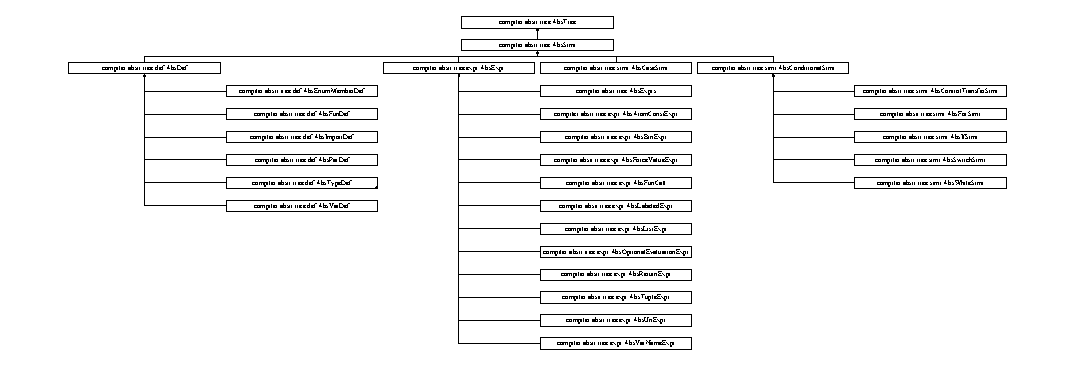
\includegraphics[height=4.472843cm]{classcompiler_1_1abstr_1_1tree_1_1_abs_stmt}
\end{center}
\end{figure}
\subsection*{Public Member Functions}
\begin{DoxyCompactItemize}
\item 
\hyperlink{classcompiler_1_1abstr_1_1tree_1_1_abs_stmt_a2e37c113e5c0d2febd88c952a15dcbee}{Abs\+Stmt} (\hyperlink{classcompiler_1_1_position}{Position} pos)
\end{DoxyCompactItemize}
\subsection*{Additional Inherited Members}


\subsection{Detailed Description}
Statement. \begin{DoxyAuthor}{Author}
toni kocjan 
\end{DoxyAuthor}


\subsection{Constructor \& Destructor Documentation}
\mbox{\Hypertarget{classcompiler_1_1abstr_1_1tree_1_1_abs_stmt_a2e37c113e5c0d2febd88c952a15dcbee}\label{classcompiler_1_1abstr_1_1tree_1_1_abs_stmt_a2e37c113e5c0d2febd88c952a15dcbee}} 
\index{compiler\+::abstr\+::tree\+::\+Abs\+Stmt@{compiler\+::abstr\+::tree\+::\+Abs\+Stmt}!Abs\+Stmt@{Abs\+Stmt}}
\index{Abs\+Stmt@{Abs\+Stmt}!compiler\+::abstr\+::tree\+::\+Abs\+Stmt@{compiler\+::abstr\+::tree\+::\+Abs\+Stmt}}
\subsubsection{\texorpdfstring{Abs\+Stmt()}{AbsStmt()}}
{\footnotesize\ttfamily compiler.\+abstr.\+tree.\+Abs\+Stmt.\+Abs\+Stmt (\begin{DoxyParamCaption}\item[{\hyperlink{classcompiler_1_1_position}{Position}}]{pos }\end{DoxyParamCaption})}

Create new statement.


\begin{DoxyParams}{Parameters}
{\em pos} & \hyperlink{classcompiler_1_1_position}{Position}. \\
\hline
\end{DoxyParams}


The documentation for this class was generated from the following file\+:\begin{DoxyCompactItemize}
\item 
src/compiler/abstr/tree/Abs\+Stmt.\+java\end{DoxyCompactItemize}

\hypertarget{classcompiler_1_1abstr_1_1tree_1_1_abs_stmts}{}\section{compiler.\+abstr.\+tree.\+Abs\+Stmts Class Reference}
\label{classcompiler_1_1abstr_1_1tree_1_1_abs_stmts}\index{compiler.\+abstr.\+tree.\+Abs\+Stmts@{compiler.\+abstr.\+tree.\+Abs\+Stmts}}
Inheritance diagram for compiler.\+abstr.\+tree.\+Abs\+Stmts\+:\begin{figure}[H]
\begin{center}
\leavevmode
\includegraphics[height=2.000000cm]{classcompiler_1_1abstr_1_1tree_1_1_abs_stmts}
\end{center}
\end{figure}
\subsection*{Public Member Functions}
\begin{DoxyCompactItemize}
\item 
\hyperlink{classcompiler_1_1abstr_1_1tree_1_1_abs_stmts_ae15c4d33cbbe4c8211323b5c07499499}{Abs\+Stmts} (\hyperlink{classcompiler_1_1_position}{Position} \hyperlink{classcompiler_1_1abstr_1_1tree_1_1_abs_tree_a127a686d3a3f9ba470f36c6b3336caea}{position}, Linked\+List$<$ \hyperlink{classcompiler_1_1abstr_1_1tree_1_1_abs_stmt}{Abs\+Stmt} $>$ abs\+Stmts)
\item 
\hyperlink{classcompiler_1_1abstr_1_1tree_1_1_abs_stmts_ad1be108e84442b930f22a7fe7e274e89}{Abs\+Stmts} (\hyperlink{classcompiler_1_1_position}{Position} \hyperlink{classcompiler_1_1abstr_1_1tree_1_1_abs_tree_a127a686d3a3f9ba470f36c6b3336caea}{position}, Linked\+List$<$ \hyperlink{classcompiler_1_1abstr_1_1tree_1_1def_1_1_abs_def}{Abs\+Def} $>$ defs, boolean ignore)
\item 
\mbox{\Hypertarget{classcompiler_1_1abstr_1_1tree_1_1_abs_stmts_a8501756490b9e386904d927288c11874}\label{classcompiler_1_1abstr_1_1tree_1_1_abs_stmts_a8501756490b9e386904d927288c11874}} 
void {\bfseries accept} (\hyperlink{interfacecompiler_1_1abstr_1_1_a_s_t_visitor}{A\+S\+T\+Visitor} a\+S\+T\+Visitor)
\end{DoxyCompactItemize}
\subsection*{Public Attributes}
\begin{DoxyCompactItemize}
\item 
final Linked\+List$<$ \hyperlink{classcompiler_1_1abstr_1_1tree_1_1_abs_stmt}{Abs\+Stmt} $>$ \hyperlink{classcompiler_1_1abstr_1_1tree_1_1_abs_stmts_acdb710e241c750ea503cb826b0de182a}{statements}
\end{DoxyCompactItemize}


\subsection{Detailed Description}
List of statements. \begin{DoxyAuthor}{Author}
toni kocjan 
\end{DoxyAuthor}


\subsection{Constructor \& Destructor Documentation}
\mbox{\Hypertarget{classcompiler_1_1abstr_1_1tree_1_1_abs_stmts_ae15c4d33cbbe4c8211323b5c07499499}\label{classcompiler_1_1abstr_1_1tree_1_1_abs_stmts_ae15c4d33cbbe4c8211323b5c07499499}} 
\index{compiler\+::abstr\+::tree\+::\+Abs\+Stmts@{compiler\+::abstr\+::tree\+::\+Abs\+Stmts}!Abs\+Stmts@{Abs\+Stmts}}
\index{Abs\+Stmts@{Abs\+Stmts}!compiler\+::abstr\+::tree\+::\+Abs\+Stmts@{compiler\+::abstr\+::tree\+::\+Abs\+Stmts}}
\subsubsection{\texorpdfstring{Abs\+Stmts()}{AbsStmts()}\hspace{0.1cm}{\footnotesize\ttfamily [1/2]}}
{\footnotesize\ttfamily compiler.\+abstr.\+tree.\+Abs\+Stmts.\+Abs\+Stmts (\begin{DoxyParamCaption}\item[{\hyperlink{classcompiler_1_1_position}{Position}}]{position,  }\item[{Linked\+List$<$ \hyperlink{classcompiler_1_1abstr_1_1tree_1_1_abs_stmt}{Abs\+Stmt} $>$}]{abs\+Stmts }\end{DoxyParamCaption})}

Create new statements list. 
\begin{DoxyParams}{Parameters}
{\em position} & \hyperlink{classcompiler_1_1_position}{Position}. \\
\hline
{\em abs\+Stmts} & Statements. \\
\hline
\end{DoxyParams}
\mbox{\Hypertarget{classcompiler_1_1abstr_1_1tree_1_1_abs_stmts_ad1be108e84442b930f22a7fe7e274e89}\label{classcompiler_1_1abstr_1_1tree_1_1_abs_stmts_ad1be108e84442b930f22a7fe7e274e89}} 
\index{compiler\+::abstr\+::tree\+::\+Abs\+Stmts@{compiler\+::abstr\+::tree\+::\+Abs\+Stmts}!Abs\+Stmts@{Abs\+Stmts}}
\index{Abs\+Stmts@{Abs\+Stmts}!compiler\+::abstr\+::tree\+::\+Abs\+Stmts@{compiler\+::abstr\+::tree\+::\+Abs\+Stmts}}
\subsubsection{\texorpdfstring{Abs\+Stmts()}{AbsStmts()}\hspace{0.1cm}{\footnotesize\ttfamily [2/2]}}
{\footnotesize\ttfamily compiler.\+abstr.\+tree.\+Abs\+Stmts.\+Abs\+Stmts (\begin{DoxyParamCaption}\item[{\hyperlink{classcompiler_1_1_position}{Position}}]{position,  }\item[{Linked\+List$<$ \hyperlink{classcompiler_1_1abstr_1_1tree_1_1def_1_1_abs_def}{Abs\+Def} $>$}]{defs,  }\item[{boolean}]{ignore }\end{DoxyParamCaption})}

Create new statements list. 
\begin{DoxyParams}{Parameters}
{\em position} & \hyperlink{classcompiler_1_1_position}{Position}. \\
\hline
{\em defs} & Definitions. \\
\hline
\end{DoxyParams}


\subsection{Member Data Documentation}
\mbox{\Hypertarget{classcompiler_1_1abstr_1_1tree_1_1_abs_stmts_acdb710e241c750ea503cb826b0de182a}\label{classcompiler_1_1abstr_1_1tree_1_1_abs_stmts_acdb710e241c750ea503cb826b0de182a}} 
\index{compiler\+::abstr\+::tree\+::\+Abs\+Stmts@{compiler\+::abstr\+::tree\+::\+Abs\+Stmts}!statements@{statements}}
\index{statements@{statements}!compiler\+::abstr\+::tree\+::\+Abs\+Stmts@{compiler\+::abstr\+::tree\+::\+Abs\+Stmts}}
\subsubsection{\texorpdfstring{statements}{statements}}
{\footnotesize\ttfamily final Linked\+List$<$\hyperlink{classcompiler_1_1abstr_1_1tree_1_1_abs_stmt}{Abs\+Stmt}$>$ compiler.\+abstr.\+tree.\+Abs\+Stmts.\+statements}

Statements. 

The documentation for this class was generated from the following file\+:\begin{DoxyCompactItemize}
\item 
src/compiler/abstr/tree/Abs\+Stmts.\+java\end{DoxyCompactItemize}

\hypertarget{classcompiler_1_1abstr_1_1tree_1_1def_1_1_abs_struct_def}{}\section{compiler.\+abstr.\+tree.\+def.\+Abs\+Struct\+Def Class Reference}
\label{classcompiler_1_1abstr_1_1tree_1_1def_1_1_abs_struct_def}\index{compiler.\+abstr.\+tree.\+def.\+Abs\+Struct\+Def@{compiler.\+abstr.\+tree.\+def.\+Abs\+Struct\+Def}}
Inheritance diagram for compiler.\+abstr.\+tree.\+def.\+Abs\+Struct\+Def\+:\begin{figure}[H]
\begin{center}
\leavevmode
\includegraphics[height=6.000000cm]{classcompiler_1_1abstr_1_1tree_1_1def_1_1_abs_struct_def}
\end{center}
\end{figure}
\subsection*{Public Member Functions}
\begin{DoxyCompactItemize}
\item 
\hyperlink{classcompiler_1_1abstr_1_1tree_1_1def_1_1_abs_struct_def_a14999b6bc00ab1658b7d052fb1fd6418}{Abs\+Struct\+Def} (String \hyperlink{classcompiler_1_1abstr_1_1tree_1_1def_1_1_abs_def_ac6bda9377f5abbb5f1be7d3d1b16481b}{name}, \hyperlink{classcompiler_1_1_position}{Position} pos, \hyperlink{classcompiler_1_1abstr_1_1tree_1_1type_1_1_abs_type}{Abs\+Type} \hyperlink{classcompiler_1_1abstr_1_1tree_1_1def_1_1_abs_class_def_abdae78a199f920488fa89f40fc123fa9}{base\+Class}, Linked\+List$<$ \hyperlink{classcompiler_1_1abstr_1_1tree_1_1def_1_1_abs_def}{Abs\+Def} $>$ \hyperlink{classcompiler_1_1abstr_1_1tree_1_1def_1_1_abs_class_def_a150268afc17218143bf4caf8a1db9c96}{definitions}, Linked\+List$<$ \hyperlink{classcompiler_1_1abstr_1_1tree_1_1_abs_stmt}{Abs\+Stmt} $>$ \hyperlink{classcompiler_1_1abstr_1_1tree_1_1def_1_1_abs_class_def_ac9a16d0a80e785164055560fc5b1c198}{default\+Constructor}, Linked\+List$<$ \hyperlink{classcompiler_1_1abstr_1_1tree_1_1def_1_1_abs_fun_def}{Abs\+Fun\+Def} $>$ constructors)
\item 
String \hyperlink{classcompiler_1_1abstr_1_1tree_1_1def_1_1_abs_struct_def_af141875c00e403614ea7ad9245fef7fc}{to\+String} ()
\end{DoxyCompactItemize}
\subsection*{Additional Inherited Members}


\subsection{Constructor \& Destructor Documentation}
\mbox{\Hypertarget{classcompiler_1_1abstr_1_1tree_1_1def_1_1_abs_struct_def_a14999b6bc00ab1658b7d052fb1fd6418}\label{classcompiler_1_1abstr_1_1tree_1_1def_1_1_abs_struct_def_a14999b6bc00ab1658b7d052fb1fd6418}} 
\index{compiler\+::abstr\+::tree\+::def\+::\+Abs\+Struct\+Def@{compiler\+::abstr\+::tree\+::def\+::\+Abs\+Struct\+Def}!Abs\+Struct\+Def@{Abs\+Struct\+Def}}
\index{Abs\+Struct\+Def@{Abs\+Struct\+Def}!compiler\+::abstr\+::tree\+::def\+::\+Abs\+Struct\+Def@{compiler\+::abstr\+::tree\+::def\+::\+Abs\+Struct\+Def}}
\subsubsection{\texorpdfstring{Abs\+Struct\+Def()}{AbsStructDef()}}
{\footnotesize\ttfamily compiler.\+abstr.\+tree.\+def.\+Abs\+Struct\+Def.\+Abs\+Struct\+Def (\begin{DoxyParamCaption}\item[{String}]{name,  }\item[{\hyperlink{classcompiler_1_1_position}{Position}}]{pos,  }\item[{\hyperlink{classcompiler_1_1abstr_1_1tree_1_1type_1_1_abs_type}{Abs\+Type}}]{base\+Class,  }\item[{Linked\+List$<$ \hyperlink{classcompiler_1_1abstr_1_1tree_1_1def_1_1_abs_def}{Abs\+Def} $>$}]{definitions,  }\item[{Linked\+List$<$ \hyperlink{classcompiler_1_1abstr_1_1tree_1_1_abs_stmt}{Abs\+Stmt} $>$}]{default\+Constructor,  }\item[{Linked\+List$<$ \hyperlink{classcompiler_1_1abstr_1_1tree_1_1def_1_1_abs_fun_def}{Abs\+Fun\+Def} $>$}]{constructors }\end{DoxyParamCaption})}


\begin{DoxyParams}{Parameters}
{\em name} & \\
\hline
{\em pos} & \\
\hline
{\em base\+Class} & \\
\hline
{\em definitions} & \\
\hline
{\em default\+Constructor} & \\
\hline
{\em constructors} & \\
\hline
\end{DoxyParams}


\subsection{Member Function Documentation}
\mbox{\Hypertarget{classcompiler_1_1abstr_1_1tree_1_1def_1_1_abs_struct_def_af141875c00e403614ea7ad9245fef7fc}\label{classcompiler_1_1abstr_1_1tree_1_1def_1_1_abs_struct_def_af141875c00e403614ea7ad9245fef7fc}} 
\index{compiler\+::abstr\+::tree\+::def\+::\+Abs\+Struct\+Def@{compiler\+::abstr\+::tree\+::def\+::\+Abs\+Struct\+Def}!to\+String@{to\+String}}
\index{to\+String@{to\+String}!compiler\+::abstr\+::tree\+::def\+::\+Abs\+Struct\+Def@{compiler\+::abstr\+::tree\+::def\+::\+Abs\+Struct\+Def}}
\subsubsection{\texorpdfstring{to\+String()}{toString()}}
{\footnotesize\ttfamily String compiler.\+abstr.\+tree.\+def.\+Abs\+Struct\+Def.\+to\+String (\begin{DoxyParamCaption}{ }\end{DoxyParamCaption})}

\begin{DoxyReturn}{Returns}

\end{DoxyReturn}


The documentation for this class was generated from the following file\+:\begin{DoxyCompactItemize}
\item 
src/compiler/abstr/tree/def/Abs\+Struct\+Def.\+java\end{DoxyCompactItemize}

\hypertarget{classcompiler_1_1abstr_1_1tree_1_1stmt_1_1_abs_switch_stmt}{}\section{compiler.\+abstr.\+tree.\+stmt.\+Abs\+Switch\+Stmt Class Reference}
\label{classcompiler_1_1abstr_1_1tree_1_1stmt_1_1_abs_switch_stmt}\index{compiler.\+abstr.\+tree.\+stmt.\+Abs\+Switch\+Stmt@{compiler.\+abstr.\+tree.\+stmt.\+Abs\+Switch\+Stmt}}
Inheritance diagram for compiler.\+abstr.\+tree.\+stmt.\+Abs\+Switch\+Stmt\+:\begin{figure}[H]
\begin{center}
\leavevmode
\includegraphics[height=4.000000cm]{classcompiler_1_1abstr_1_1tree_1_1stmt_1_1_abs_switch_stmt}
\end{center}
\end{figure}
\subsection*{Public Member Functions}
\begin{DoxyCompactItemize}
\item 
\hyperlink{classcompiler_1_1abstr_1_1tree_1_1stmt_1_1_abs_switch_stmt_a467cbc851d97d21688f1378d7d8e13e6}{Abs\+Switch\+Stmt} (\hyperlink{classcompiler_1_1_position}{Position} pos, \hyperlink{classcompiler_1_1abstr_1_1tree_1_1expr_1_1_abs_expr}{Abs\+Expr} \hyperlink{classcompiler_1_1abstr_1_1tree_1_1stmt_1_1_abs_switch_stmt_a827d963b0b450513c19919645d325a81}{subject\+Expr}, Vector$<$ \hyperlink{classcompiler_1_1abstr_1_1tree_1_1stmt_1_1_abs_case_stmt}{Abs\+Case\+Stmt} $>$ \hyperlink{classcompiler_1_1abstr_1_1tree_1_1stmt_1_1_abs_switch_stmt_a471b6f000fe299a92e2135f1a3921f12}{cases}, \hyperlink{classcompiler_1_1abstr_1_1tree_1_1_abs_stmts}{Abs\+Stmts} \hyperlink{classcompiler_1_1abstr_1_1tree_1_1stmt_1_1_abs_switch_stmt_a2a8600e70568fe111d8a3e53a31a3516}{default\+Body})
\item 
\mbox{\Hypertarget{classcompiler_1_1abstr_1_1tree_1_1stmt_1_1_abs_switch_stmt_a939eb2b4c2ae81b481acc1ae2b5086a7}\label{classcompiler_1_1abstr_1_1tree_1_1stmt_1_1_abs_switch_stmt_a939eb2b4c2ae81b481acc1ae2b5086a7}} 
void {\bfseries accept} (\hyperlink{interfacecompiler_1_1abstr_1_1_a_s_t_visitor}{A\+S\+T\+Visitor} a\+S\+T\+Visitor)
\end{DoxyCompactItemize}
\subsection*{Public Attributes}
\begin{DoxyCompactItemize}
\item 
final \hyperlink{classcompiler_1_1abstr_1_1tree_1_1expr_1_1_abs_expr}{Abs\+Expr} \hyperlink{classcompiler_1_1abstr_1_1tree_1_1stmt_1_1_abs_switch_stmt_a827d963b0b450513c19919645d325a81}{subject\+Expr}
\item 
final Vector$<$ \hyperlink{classcompiler_1_1abstr_1_1tree_1_1stmt_1_1_abs_case_stmt}{Abs\+Case\+Stmt} $>$ \hyperlink{classcompiler_1_1abstr_1_1tree_1_1stmt_1_1_abs_switch_stmt_a471b6f000fe299a92e2135f1a3921f12}{cases}
\item 
final \hyperlink{classcompiler_1_1abstr_1_1tree_1_1_abs_stmts}{Abs\+Stmts} \hyperlink{classcompiler_1_1abstr_1_1tree_1_1stmt_1_1_abs_switch_stmt_a2a8600e70568fe111d8a3e53a31a3516}{default\+Body}
\end{DoxyCompactItemize}


\subsection{Constructor \& Destructor Documentation}
\mbox{\Hypertarget{classcompiler_1_1abstr_1_1tree_1_1stmt_1_1_abs_switch_stmt_a467cbc851d97d21688f1378d7d8e13e6}\label{classcompiler_1_1abstr_1_1tree_1_1stmt_1_1_abs_switch_stmt_a467cbc851d97d21688f1378d7d8e13e6}} 
\index{compiler\+::abstr\+::tree\+::stmt\+::\+Abs\+Switch\+Stmt@{compiler\+::abstr\+::tree\+::stmt\+::\+Abs\+Switch\+Stmt}!Abs\+Switch\+Stmt@{Abs\+Switch\+Stmt}}
\index{Abs\+Switch\+Stmt@{Abs\+Switch\+Stmt}!compiler\+::abstr\+::tree\+::stmt\+::\+Abs\+Switch\+Stmt@{compiler\+::abstr\+::tree\+::stmt\+::\+Abs\+Switch\+Stmt}}
\subsubsection{\texorpdfstring{Abs\+Switch\+Stmt()}{AbsSwitchStmt()}}
{\footnotesize\ttfamily compiler.\+abstr.\+tree.\+stmt.\+Abs\+Switch\+Stmt.\+Abs\+Switch\+Stmt (\begin{DoxyParamCaption}\item[{\hyperlink{classcompiler_1_1_position}{Position}}]{pos,  }\item[{\hyperlink{classcompiler_1_1abstr_1_1tree_1_1expr_1_1_abs_expr}{Abs\+Expr}}]{subject\+Expr,  }\item[{Vector$<$ \hyperlink{classcompiler_1_1abstr_1_1tree_1_1stmt_1_1_abs_case_stmt}{Abs\+Case\+Stmt} $>$}]{cases,  }\item[{\hyperlink{classcompiler_1_1abstr_1_1tree_1_1_abs_stmts}{Abs\+Stmts}}]{default\+Body }\end{DoxyParamCaption})}


\begin{DoxyParams}{Parameters}
{\em pos} & \\
\hline
\end{DoxyParams}


\subsection{Member Data Documentation}
\mbox{\Hypertarget{classcompiler_1_1abstr_1_1tree_1_1stmt_1_1_abs_switch_stmt_a471b6f000fe299a92e2135f1a3921f12}\label{classcompiler_1_1abstr_1_1tree_1_1stmt_1_1_abs_switch_stmt_a471b6f000fe299a92e2135f1a3921f12}} 
\index{compiler\+::abstr\+::tree\+::stmt\+::\+Abs\+Switch\+Stmt@{compiler\+::abstr\+::tree\+::stmt\+::\+Abs\+Switch\+Stmt}!cases@{cases}}
\index{cases@{cases}!compiler\+::abstr\+::tree\+::stmt\+::\+Abs\+Switch\+Stmt@{compiler\+::abstr\+::tree\+::stmt\+::\+Abs\+Switch\+Stmt}}
\subsubsection{\texorpdfstring{cases}{cases}}
{\footnotesize\ttfamily final Vector$<$\hyperlink{classcompiler_1_1abstr_1_1tree_1_1stmt_1_1_abs_case_stmt}{Abs\+Case\+Stmt}$>$ compiler.\+abstr.\+tree.\+stmt.\+Abs\+Switch\+Stmt.\+cases}

Cases. \mbox{\Hypertarget{classcompiler_1_1abstr_1_1tree_1_1stmt_1_1_abs_switch_stmt_a2a8600e70568fe111d8a3e53a31a3516}\label{classcompiler_1_1abstr_1_1tree_1_1stmt_1_1_abs_switch_stmt_a2a8600e70568fe111d8a3e53a31a3516}} 
\index{compiler\+::abstr\+::tree\+::stmt\+::\+Abs\+Switch\+Stmt@{compiler\+::abstr\+::tree\+::stmt\+::\+Abs\+Switch\+Stmt}!default\+Body@{default\+Body}}
\index{default\+Body@{default\+Body}!compiler\+::abstr\+::tree\+::stmt\+::\+Abs\+Switch\+Stmt@{compiler\+::abstr\+::tree\+::stmt\+::\+Abs\+Switch\+Stmt}}
\subsubsection{\texorpdfstring{default\+Body}{defaultBody}}
{\footnotesize\ttfamily final \hyperlink{classcompiler_1_1abstr_1_1tree_1_1_abs_stmts}{Abs\+Stmts} compiler.\+abstr.\+tree.\+stmt.\+Abs\+Switch\+Stmt.\+default\+Body}

Default body code. \mbox{\Hypertarget{classcompiler_1_1abstr_1_1tree_1_1stmt_1_1_abs_switch_stmt_a827d963b0b450513c19919645d325a81}\label{classcompiler_1_1abstr_1_1tree_1_1stmt_1_1_abs_switch_stmt_a827d963b0b450513c19919645d325a81}} 
\index{compiler\+::abstr\+::tree\+::stmt\+::\+Abs\+Switch\+Stmt@{compiler\+::abstr\+::tree\+::stmt\+::\+Abs\+Switch\+Stmt}!subject\+Expr@{subject\+Expr}}
\index{subject\+Expr@{subject\+Expr}!compiler\+::abstr\+::tree\+::stmt\+::\+Abs\+Switch\+Stmt@{compiler\+::abstr\+::tree\+::stmt\+::\+Abs\+Switch\+Stmt}}
\subsubsection{\texorpdfstring{subject\+Expr}{subjectExpr}}
{\footnotesize\ttfamily final \hyperlink{classcompiler_1_1abstr_1_1tree_1_1expr_1_1_abs_expr}{Abs\+Expr} compiler.\+abstr.\+tree.\+stmt.\+Abs\+Switch\+Stmt.\+subject\+Expr}

Expression to be compared. Must be typed as Int, String (or Enum) 

The documentation for this class was generated from the following file\+:\begin{DoxyCompactItemize}
\item 
src/compiler/abstr/tree/stmt/Abs\+Switch\+Stmt.\+java\end{DoxyCompactItemize}

\hypertarget{classcompiler_1_1abstr_1_1tree_1_1_abs_tree}{}\section{compiler.\+abstr.\+tree.\+Abs\+Tree Class Reference}
\label{classcompiler_1_1abstr_1_1tree_1_1_abs_tree}\index{compiler.\+abstr.\+tree.\+Abs\+Tree@{compiler.\+abstr.\+tree.\+Abs\+Tree}}
Inheritance diagram for compiler.\+abstr.\+tree.\+Abs\+Tree\+:\begin{figure}[H]
\begin{center}
\leavevmode
\includegraphics[height=2.980989cm]{classcompiler_1_1abstr_1_1tree_1_1_abs_tree}
\end{center}
\end{figure}
\subsection*{Public Member Functions}
\begin{DoxyCompactItemize}
\item 
\hyperlink{classcompiler_1_1abstr_1_1tree_1_1_abs_tree_a4685afe81da918ece73cdcac477c810c}{Abs\+Tree} (\hyperlink{classcompiler_1_1_position}{Position} pos)
\item 
\mbox{\Hypertarget{classcompiler_1_1abstr_1_1tree_1_1_abs_tree_adc0914a591fdf026f83d51bbe2c8cf55}\label{classcompiler_1_1abstr_1_1tree_1_1_abs_tree_adc0914a591fdf026f83d51bbe2c8cf55}} 
abstract void {\bfseries accept} (\hyperlink{interfacecompiler_1_1abstr_1_1_a_s_t_visitor}{A\+S\+T\+Visitor} a\+S\+T\+Visitor)
\end{DoxyCompactItemize}
\subsection*{Public Attributes}
\begin{DoxyCompactItemize}
\item 
final \hyperlink{classcompiler_1_1_position}{Position} \hyperlink{classcompiler_1_1abstr_1_1tree_1_1_abs_tree_a127a686d3a3f9ba470f36c6b3336caea}{position}
\end{DoxyCompactItemize}


\subsection{Detailed Description}
Abstract syntax tree node. This is base class for all types of nodes.

\begin{DoxyAuthor}{Author}
toni kocjan 
\end{DoxyAuthor}


\subsection{Constructor \& Destructor Documentation}
\mbox{\Hypertarget{classcompiler_1_1abstr_1_1tree_1_1_abs_tree_a4685afe81da918ece73cdcac477c810c}\label{classcompiler_1_1abstr_1_1tree_1_1_abs_tree_a4685afe81da918ece73cdcac477c810c}} 
\index{compiler\+::abstr\+::tree\+::\+Abs\+Tree@{compiler\+::abstr\+::tree\+::\+Abs\+Tree}!Abs\+Tree@{Abs\+Tree}}
\index{Abs\+Tree@{Abs\+Tree}!compiler\+::abstr\+::tree\+::\+Abs\+Tree@{compiler\+::abstr\+::tree\+::\+Abs\+Tree}}
\subsubsection{\texorpdfstring{Abs\+Tree()}{AbsTree()}}
{\footnotesize\ttfamily compiler.\+abstr.\+tree.\+Abs\+Tree.\+Abs\+Tree (\begin{DoxyParamCaption}\item[{\hyperlink{classcompiler_1_1_position}{Position}}]{pos }\end{DoxyParamCaption})}

Create new abstract syntax tree.


\begin{DoxyParams}{Parameters}
{\em pos} & \hyperlink{classcompiler_1_1_position}{Position}. \\
\hline
\end{DoxyParams}


\subsection{Member Data Documentation}
\mbox{\Hypertarget{classcompiler_1_1abstr_1_1tree_1_1_abs_tree_a127a686d3a3f9ba470f36c6b3336caea}\label{classcompiler_1_1abstr_1_1tree_1_1_abs_tree_a127a686d3a3f9ba470f36c6b3336caea}} 
\index{compiler\+::abstr\+::tree\+::\+Abs\+Tree@{compiler\+::abstr\+::tree\+::\+Abs\+Tree}!position@{position}}
\index{position@{position}!compiler\+::abstr\+::tree\+::\+Abs\+Tree@{compiler\+::abstr\+::tree\+::\+Abs\+Tree}}
\subsubsection{\texorpdfstring{position}{position}}
{\footnotesize\ttfamily final \hyperlink{classcompiler_1_1_position}{Position} compiler.\+abstr.\+tree.\+Abs\+Tree.\+position}

\hyperlink{classcompiler_1_1_position}{Position} of this node. 

The documentation for this class was generated from the following file\+:\begin{DoxyCompactItemize}
\item 
src/compiler/abstr/tree/Abs\+Tree.\+java\end{DoxyCompactItemize}

\hypertarget{classcompiler_1_1abstr_1_1tree_1_1def_1_1_abs_tuple_def}{}\section{compiler.\+abstr.\+tree.\+def.\+Abs\+Tuple\+Def Class Reference}
\label{classcompiler_1_1abstr_1_1tree_1_1def_1_1_abs_tuple_def}\index{compiler.\+abstr.\+tree.\+def.\+Abs\+Tuple\+Def@{compiler.\+abstr.\+tree.\+def.\+Abs\+Tuple\+Def}}
Inheritance diagram for compiler.\+abstr.\+tree.\+def.\+Abs\+Tuple\+Def\+:\begin{figure}[H]
\begin{center}
\leavevmode
\includegraphics[height=5.000000cm]{classcompiler_1_1abstr_1_1tree_1_1def_1_1_abs_tuple_def}
\end{center}
\end{figure}
\subsection*{Public Member Functions}
\begin{DoxyCompactItemize}
\item 
\hyperlink{classcompiler_1_1abstr_1_1tree_1_1def_1_1_abs_tuple_def_a6d11bf4078808721e03332c9a0ec8272}{Abs\+Tuple\+Def} (\hyperlink{classcompiler_1_1_position}{Position} pos, Linked\+List$<$ \hyperlink{classcompiler_1_1abstr_1_1tree_1_1def_1_1_abs_def}{Abs\+Def} $>$ defs)
\item 
\mbox{\Hypertarget{classcompiler_1_1abstr_1_1tree_1_1def_1_1_abs_tuple_def_af6089a2fce7fb394ab11ead2c2e893cc}\label{classcompiler_1_1abstr_1_1tree_1_1def_1_1_abs_tuple_def_af6089a2fce7fb394ab11ead2c2e893cc}} 
void {\bfseries accept} (\hyperlink{interfacecompiler_1_1abstr_1_1_a_s_t_visitor}{A\+S\+T\+Visitor} a\+S\+T\+Visitor)
\end{DoxyCompactItemize}
\subsection*{Public Attributes}
\begin{DoxyCompactItemize}
\item 
final \hyperlink{classcompiler_1_1abstr_1_1tree_1_1_abs_defs}{Abs\+Defs} \hyperlink{classcompiler_1_1abstr_1_1tree_1_1def_1_1_abs_tuple_def_a7c764c8a266ea4b139b64f59377a5082}{definitions}
\end{DoxyCompactItemize}
\subsection*{Additional Inherited Members}


\subsection{Detailed Description}
Tuple definition. \begin{DoxyAuthor}{Author}
toni kocjan 
\end{DoxyAuthor}


\subsection{Constructor \& Destructor Documentation}
\mbox{\Hypertarget{classcompiler_1_1abstr_1_1tree_1_1def_1_1_abs_tuple_def_a6d11bf4078808721e03332c9a0ec8272}\label{classcompiler_1_1abstr_1_1tree_1_1def_1_1_abs_tuple_def_a6d11bf4078808721e03332c9a0ec8272}} 
\index{compiler\+::abstr\+::tree\+::def\+::\+Abs\+Tuple\+Def@{compiler\+::abstr\+::tree\+::def\+::\+Abs\+Tuple\+Def}!Abs\+Tuple\+Def@{Abs\+Tuple\+Def}}
\index{Abs\+Tuple\+Def@{Abs\+Tuple\+Def}!compiler\+::abstr\+::tree\+::def\+::\+Abs\+Tuple\+Def@{compiler\+::abstr\+::tree\+::def\+::\+Abs\+Tuple\+Def}}
\subsubsection{\texorpdfstring{Abs\+Tuple\+Def()}{AbsTupleDef()}}
{\footnotesize\ttfamily compiler.\+abstr.\+tree.\+def.\+Abs\+Tuple\+Def.\+Abs\+Tuple\+Def (\begin{DoxyParamCaption}\item[{\hyperlink{classcompiler_1_1_position}{Position}}]{pos,  }\item[{Linked\+List$<$ \hyperlink{classcompiler_1_1abstr_1_1tree_1_1def_1_1_abs_def}{Abs\+Def} $>$}]{defs }\end{DoxyParamCaption})}

Create new tuple type definition 
\begin{DoxyParams}{Parameters}
{\em pos} & position \\
\hline
{\em defs} & member definitions \\
\hline
\end{DoxyParams}


\subsection{Member Data Documentation}
\mbox{\Hypertarget{classcompiler_1_1abstr_1_1tree_1_1def_1_1_abs_tuple_def_a7c764c8a266ea4b139b64f59377a5082}\label{classcompiler_1_1abstr_1_1tree_1_1def_1_1_abs_tuple_def_a7c764c8a266ea4b139b64f59377a5082}} 
\index{compiler\+::abstr\+::tree\+::def\+::\+Abs\+Tuple\+Def@{compiler\+::abstr\+::tree\+::def\+::\+Abs\+Tuple\+Def}!definitions@{definitions}}
\index{definitions@{definitions}!compiler\+::abstr\+::tree\+::def\+::\+Abs\+Tuple\+Def@{compiler\+::abstr\+::tree\+::def\+::\+Abs\+Tuple\+Def}}
\subsubsection{\texorpdfstring{definitions}{definitions}}
{\footnotesize\ttfamily final \hyperlink{classcompiler_1_1abstr_1_1tree_1_1_abs_defs}{Abs\+Defs} compiler.\+abstr.\+tree.\+def.\+Abs\+Tuple\+Def.\+definitions}

Definitions inside tuple 

The documentation for this class was generated from the following file\+:\begin{DoxyCompactItemize}
\item 
src/compiler/abstr/tree/def/Abs\+Tuple\+Def.\+java\end{DoxyCompactItemize}

\hypertarget{classcompiler_1_1abstr_1_1tree_1_1expr_1_1_abs_tuple_expr}{}\section{compiler.\+abstr.\+tree.\+expr.\+Abs\+Tuple\+Expr Class Reference}
\label{classcompiler_1_1abstr_1_1tree_1_1expr_1_1_abs_tuple_expr}\index{compiler.\+abstr.\+tree.\+expr.\+Abs\+Tuple\+Expr@{compiler.\+abstr.\+tree.\+expr.\+Abs\+Tuple\+Expr}}
Inheritance diagram for compiler.\+abstr.\+tree.\+expr.\+Abs\+Tuple\+Expr\+:\begin{figure}[H]
\begin{center}
\leavevmode
\includegraphics[height=4.000000cm]{classcompiler_1_1abstr_1_1tree_1_1expr_1_1_abs_tuple_expr}
\end{center}
\end{figure}
\subsection*{Public Member Functions}
\begin{DoxyCompactItemize}
\item 
\hyperlink{classcompiler_1_1abstr_1_1tree_1_1expr_1_1_abs_tuple_expr_a4ee5fcd6edb36f4ed91fb6250d1b4997}{Abs\+Tuple\+Expr} (\hyperlink{classcompiler_1_1_position}{Position} pos, Linked\+List$<$ \hyperlink{classcompiler_1_1abstr_1_1tree_1_1expr_1_1_abs_expr}{Abs\+Expr} $>$ \hyperlink{classcompiler_1_1abstr_1_1tree_1_1expr_1_1_abs_tuple_expr_a2914b1e474a0a2013b798297e1fc4be3}{expressions})
\item 
\mbox{\Hypertarget{classcompiler_1_1abstr_1_1tree_1_1expr_1_1_abs_tuple_expr_a0a89fde38b2aa24d9af3f9e4a5dc35e1}\label{classcompiler_1_1abstr_1_1tree_1_1expr_1_1_abs_tuple_expr_a0a89fde38b2aa24d9af3f9e4a5dc35e1}} 
void {\bfseries accept} (\hyperlink{interfacecompiler_1_1abstr_1_1_a_s_t_visitor}{A\+S\+T\+Visitor} a\+S\+T\+Visitor)
\end{DoxyCompactItemize}
\subsection*{Public Attributes}
\begin{DoxyCompactItemize}
\item 
final \hyperlink{classcompiler_1_1abstr_1_1tree_1_1_abs_exprs}{Abs\+Exprs} \hyperlink{classcompiler_1_1abstr_1_1tree_1_1expr_1_1_abs_tuple_expr_a2914b1e474a0a2013b798297e1fc4be3}{expressions}
\end{DoxyCompactItemize}


\subsection{Constructor \& Destructor Documentation}
\mbox{\Hypertarget{classcompiler_1_1abstr_1_1tree_1_1expr_1_1_abs_tuple_expr_a4ee5fcd6edb36f4ed91fb6250d1b4997}\label{classcompiler_1_1abstr_1_1tree_1_1expr_1_1_abs_tuple_expr_a4ee5fcd6edb36f4ed91fb6250d1b4997}} 
\index{compiler\+::abstr\+::tree\+::expr\+::\+Abs\+Tuple\+Expr@{compiler\+::abstr\+::tree\+::expr\+::\+Abs\+Tuple\+Expr}!Abs\+Tuple\+Expr@{Abs\+Tuple\+Expr}}
\index{Abs\+Tuple\+Expr@{Abs\+Tuple\+Expr}!compiler\+::abstr\+::tree\+::expr\+::\+Abs\+Tuple\+Expr@{compiler\+::abstr\+::tree\+::expr\+::\+Abs\+Tuple\+Expr}}
\subsubsection{\texorpdfstring{Abs\+Tuple\+Expr()}{AbsTupleExpr()}}
{\footnotesize\ttfamily compiler.\+abstr.\+tree.\+expr.\+Abs\+Tuple\+Expr.\+Abs\+Tuple\+Expr (\begin{DoxyParamCaption}\item[{\hyperlink{classcompiler_1_1_position}{Position}}]{pos,  }\item[{Linked\+List$<$ \hyperlink{classcompiler_1_1abstr_1_1tree_1_1expr_1_1_abs_expr}{Abs\+Expr} $>$}]{expressions }\end{DoxyParamCaption})}

Create new tuple expression. 
\begin{DoxyParams}{Parameters}
{\em pos} & \\
\hline
{\em expressions} & \\
\hline
\end{DoxyParams}


\subsection{Member Data Documentation}
\mbox{\Hypertarget{classcompiler_1_1abstr_1_1tree_1_1expr_1_1_abs_tuple_expr_a2914b1e474a0a2013b798297e1fc4be3}\label{classcompiler_1_1abstr_1_1tree_1_1expr_1_1_abs_tuple_expr_a2914b1e474a0a2013b798297e1fc4be3}} 
\index{compiler\+::abstr\+::tree\+::expr\+::\+Abs\+Tuple\+Expr@{compiler\+::abstr\+::tree\+::expr\+::\+Abs\+Tuple\+Expr}!expressions@{expressions}}
\index{expressions@{expressions}!compiler\+::abstr\+::tree\+::expr\+::\+Abs\+Tuple\+Expr@{compiler\+::abstr\+::tree\+::expr\+::\+Abs\+Tuple\+Expr}}
\subsubsection{\texorpdfstring{expressions}{expressions}}
{\footnotesize\ttfamily final \hyperlink{classcompiler_1_1abstr_1_1tree_1_1_abs_exprs}{Abs\+Exprs} compiler.\+abstr.\+tree.\+expr.\+Abs\+Tuple\+Expr.\+expressions}

Expressions inside tuple expression. 

The documentation for this class was generated from the following file\+:\begin{DoxyCompactItemize}
\item 
src/compiler/abstr/tree/expr/Abs\+Tuple\+Expr.\+java\end{DoxyCompactItemize}

\hypertarget{classcompiler_1_1abstr_1_1tree_1_1type_1_1_abs_type}{}\section{compiler.\+abstr.\+tree.\+type.\+Abs\+Type Class Reference}
\label{classcompiler_1_1abstr_1_1tree_1_1type_1_1_abs_type}\index{compiler.\+abstr.\+tree.\+type.\+Abs\+Type@{compiler.\+abstr.\+tree.\+type.\+Abs\+Type}}
Inheritance diagram for compiler.\+abstr.\+tree.\+type.\+Abs\+Type\+:\begin{figure}[H]
\begin{center}
\leavevmode
\includegraphics[height=1.317647cm]{classcompiler_1_1abstr_1_1tree_1_1type_1_1_abs_type}
\end{center}
\end{figure}
\subsection*{Public Member Functions}
\begin{DoxyCompactItemize}
\item 
\hyperlink{classcompiler_1_1abstr_1_1tree_1_1type_1_1_abs_type_a64811f8d0e3e5e77f13c51aed4ec9343}{Abs\+Type} (\hyperlink{classcompiler_1_1_position}{Position} pos)
\item 
\mbox{\Hypertarget{classcompiler_1_1abstr_1_1tree_1_1type_1_1_abs_type_a8a4322a5e47357fec094931dc85ec9b8}\label{classcompiler_1_1abstr_1_1tree_1_1type_1_1_abs_type_a8a4322a5e47357fec094931dc85ec9b8}} 
abstract String {\bfseries get\+Name} ()
\end{DoxyCompactItemize}
\subsection*{Additional Inherited Members}


\subsection{Detailed Description}
Opis podatkovnega tipa.

\begin{DoxyAuthor}{Author}
sliva 
\end{DoxyAuthor}


\subsection{Constructor \& Destructor Documentation}
\mbox{\Hypertarget{classcompiler_1_1abstr_1_1tree_1_1type_1_1_abs_type_a64811f8d0e3e5e77f13c51aed4ec9343}\label{classcompiler_1_1abstr_1_1tree_1_1type_1_1_abs_type_a64811f8d0e3e5e77f13c51aed4ec9343}} 
\index{compiler\+::abstr\+::tree\+::type\+::\+Abs\+Type@{compiler\+::abstr\+::tree\+::type\+::\+Abs\+Type}!Abs\+Type@{Abs\+Type}}
\index{Abs\+Type@{Abs\+Type}!compiler\+::abstr\+::tree\+::type\+::\+Abs\+Type@{compiler\+::abstr\+::tree\+::type\+::\+Abs\+Type}}
\subsubsection{\texorpdfstring{Abs\+Type()}{AbsType()}}
{\footnotesize\ttfamily compiler.\+abstr.\+tree.\+type.\+Abs\+Type.\+Abs\+Type (\begin{DoxyParamCaption}\item[{\hyperlink{classcompiler_1_1_position}{Position}}]{pos }\end{DoxyParamCaption})}

Ustvari nov opis podatkovnega tipa.


\begin{DoxyParams}{Parameters}
{\em pos} & Polozaj stavcne oblike tega drevesa. \\
\hline
\end{DoxyParams}


The documentation for this class was generated from the following file\+:\begin{DoxyCompactItemize}
\item 
src/compiler/abstr/tree/type/Abs\+Type.\+java\end{DoxyCompactItemize}

\hypertarget{classcompiler_1_1abstr_1_1tree_1_1def_1_1_abs_type_def}{}\section{compiler.\+abstr.\+tree.\+def.\+Abs\+Type\+Def Class Reference}
\label{classcompiler_1_1abstr_1_1tree_1_1def_1_1_abs_type_def}\index{compiler.\+abstr.\+tree.\+def.\+Abs\+Type\+Def@{compiler.\+abstr.\+tree.\+def.\+Abs\+Type\+Def}}
Inheritance diagram for compiler.\+abstr.\+tree.\+def.\+Abs\+Type\+Def\+:\begin{figure}[H]
\begin{center}
\leavevmode
\includegraphics[height=2.709677cm]{classcompiler_1_1abstr_1_1tree_1_1def_1_1_abs_type_def}
\end{center}
\end{figure}
\subsection*{Public Member Functions}
\begin{DoxyCompactItemize}
\item 
\hyperlink{classcompiler_1_1abstr_1_1tree_1_1def_1_1_abs_type_def_a876cefb9eaa4874f75fda0c834c83310}{Abs\+Type\+Def} (\hyperlink{classcompiler_1_1_position}{Position} pos, String \hyperlink{classcompiler_1_1abstr_1_1tree_1_1def_1_1_abs_def_ac6bda9377f5abbb5f1be7d3d1b16481b}{name})
\end{DoxyCompactItemize}
\subsection*{Additional Inherited Members}


\subsection{Detailed Description}
Definicija tipa.

\begin{DoxyAuthor}{Author}
sliva 
\end{DoxyAuthor}


\subsection{Constructor \& Destructor Documentation}
\mbox{\Hypertarget{classcompiler_1_1abstr_1_1tree_1_1def_1_1_abs_type_def_a876cefb9eaa4874f75fda0c834c83310}\label{classcompiler_1_1abstr_1_1tree_1_1def_1_1_abs_type_def_a876cefb9eaa4874f75fda0c834c83310}} 
\index{compiler\+::abstr\+::tree\+::def\+::\+Abs\+Type\+Def@{compiler\+::abstr\+::tree\+::def\+::\+Abs\+Type\+Def}!Abs\+Type\+Def@{Abs\+Type\+Def}}
\index{Abs\+Type\+Def@{Abs\+Type\+Def}!compiler\+::abstr\+::tree\+::def\+::\+Abs\+Type\+Def@{compiler\+::abstr\+::tree\+::def\+::\+Abs\+Type\+Def}}
\subsubsection{\texorpdfstring{Abs\+Type\+Def()}{AbsTypeDef()}}
{\footnotesize\ttfamily compiler.\+abstr.\+tree.\+def.\+Abs\+Type\+Def.\+Abs\+Type\+Def (\begin{DoxyParamCaption}\item[{\hyperlink{classcompiler_1_1_position}{Position}}]{pos,  }\item[{String}]{name }\end{DoxyParamCaption})}

Ustvari novo definicijo tipa.


\begin{DoxyParams}{Parameters}
{\em pos} & Polozaj stavcne oblike tega drevesa. \\
\hline
{\em name} & Ime tipa. \\
\hline
\end{DoxyParams}


The documentation for this class was generated from the following file\+:\begin{DoxyCompactItemize}
\item 
src/compiler/abstr/tree/def/Abs\+Type\+Def.\+java\end{DoxyCompactItemize}

\hypertarget{classcompiler_1_1abstr_1_1tree_1_1type_1_1_abs_type_name}{}\section{compiler.\+abstr.\+tree.\+type.\+Abs\+Type\+Name Class Reference}
\label{classcompiler_1_1abstr_1_1tree_1_1type_1_1_abs_type_name}\index{compiler.\+abstr.\+tree.\+type.\+Abs\+Type\+Name@{compiler.\+abstr.\+tree.\+type.\+Abs\+Type\+Name}}
Inheritance diagram for compiler.\+abstr.\+tree.\+type.\+Abs\+Type\+Name\+:\begin{figure}[H]
\begin{center}
\leavevmode
\includegraphics[height=3.000000cm]{classcompiler_1_1abstr_1_1tree_1_1type_1_1_abs_type_name}
\end{center}
\end{figure}
\subsection*{Public Member Functions}
\begin{DoxyCompactItemize}
\item 
\hyperlink{classcompiler_1_1abstr_1_1tree_1_1type_1_1_abs_type_name_a38f4c0c37de6e29bcfe47266025d2b4b}{Abs\+Type\+Name} (\hyperlink{classcompiler_1_1_position}{Position} pos, String \hyperlink{classcompiler_1_1abstr_1_1tree_1_1type_1_1_abs_type_name_a41a111c2c38fc5178c2160497a7bb017}{name})
\item 
\mbox{\Hypertarget{classcompiler_1_1abstr_1_1tree_1_1type_1_1_abs_type_name_a348cc77bbbdef2353f21116c6e38a001}\label{classcompiler_1_1abstr_1_1tree_1_1type_1_1_abs_type_name_a348cc77bbbdef2353f21116c6e38a001}} 
String {\bfseries to\+String} ()
\item 
\mbox{\Hypertarget{classcompiler_1_1abstr_1_1tree_1_1type_1_1_abs_type_name_a8877f1b59a3697d03836a45069e93700}\label{classcompiler_1_1abstr_1_1tree_1_1type_1_1_abs_type_name_a8877f1b59a3697d03836a45069e93700}} 
void {\bfseries accept} (\hyperlink{interfacecompiler_1_1abstr_1_1_a_s_t_visitor}{A\+S\+T\+Visitor} a\+S\+T\+Visitor)
\item 
\mbox{\Hypertarget{classcompiler_1_1abstr_1_1tree_1_1type_1_1_abs_type_name_a1586a5b665d7d394758e7386aee5f37a}\label{classcompiler_1_1abstr_1_1tree_1_1type_1_1_abs_type_name_a1586a5b665d7d394758e7386aee5f37a}} 
String {\bfseries get\+Name} ()
\end{DoxyCompactItemize}
\subsection*{Public Attributes}
\begin{DoxyCompactItemize}
\item 
final String \hyperlink{classcompiler_1_1abstr_1_1tree_1_1type_1_1_abs_type_name_a41a111c2c38fc5178c2160497a7bb017}{name}
\end{DoxyCompactItemize}


\subsection{Detailed Description}
Opis imena tipa.

\begin{DoxyAuthor}{Author}
sliva 
\end{DoxyAuthor}


\subsection{Constructor \& Destructor Documentation}
\mbox{\Hypertarget{classcompiler_1_1abstr_1_1tree_1_1type_1_1_abs_type_name_a38f4c0c37de6e29bcfe47266025d2b4b}\label{classcompiler_1_1abstr_1_1tree_1_1type_1_1_abs_type_name_a38f4c0c37de6e29bcfe47266025d2b4b}} 
\index{compiler\+::abstr\+::tree\+::type\+::\+Abs\+Type\+Name@{compiler\+::abstr\+::tree\+::type\+::\+Abs\+Type\+Name}!Abs\+Type\+Name@{Abs\+Type\+Name}}
\index{Abs\+Type\+Name@{Abs\+Type\+Name}!compiler\+::abstr\+::tree\+::type\+::\+Abs\+Type\+Name@{compiler\+::abstr\+::tree\+::type\+::\+Abs\+Type\+Name}}
\subsubsection{\texorpdfstring{Abs\+Type\+Name()}{AbsTypeName()}}
{\footnotesize\ttfamily compiler.\+abstr.\+tree.\+type.\+Abs\+Type\+Name.\+Abs\+Type\+Name (\begin{DoxyParamCaption}\item[{\hyperlink{classcompiler_1_1_position}{Position}}]{pos,  }\item[{String}]{name }\end{DoxyParamCaption})}

Ustvari nov opis imena tipa.


\begin{DoxyParams}{Parameters}
{\em pos} & Polozaj stavcne oblike tega drevesa. \\
\hline
{\em name} & Ime tipa. \\
\hline
\end{DoxyParams}


\subsection{Member Data Documentation}
\mbox{\Hypertarget{classcompiler_1_1abstr_1_1tree_1_1type_1_1_abs_type_name_a41a111c2c38fc5178c2160497a7bb017}\label{classcompiler_1_1abstr_1_1tree_1_1type_1_1_abs_type_name_a41a111c2c38fc5178c2160497a7bb017}} 
\index{compiler\+::abstr\+::tree\+::type\+::\+Abs\+Type\+Name@{compiler\+::abstr\+::tree\+::type\+::\+Abs\+Type\+Name}!name@{name}}
\index{name@{name}!compiler\+::abstr\+::tree\+::type\+::\+Abs\+Type\+Name@{compiler\+::abstr\+::tree\+::type\+::\+Abs\+Type\+Name}}
\subsubsection{\texorpdfstring{name}{name}}
{\footnotesize\ttfamily final String compiler.\+abstr.\+tree.\+type.\+Abs\+Type\+Name.\+name}

Ime tipa. 

The documentation for this class was generated from the following file\+:\begin{DoxyCompactItemize}
\item 
src/compiler/abstr/tree/type/Abs\+Type\+Name.\+java\end{DoxyCompactItemize}

\hypertarget{classcompiler_1_1abstr_1_1tree_1_1expr_1_1_abs_un_expr}{}\section{compiler.\+abstr.\+tree.\+expr.\+Abs\+Un\+Expr Class Reference}
\label{classcompiler_1_1abstr_1_1tree_1_1expr_1_1_abs_un_expr}\index{compiler.\+abstr.\+tree.\+expr.\+Abs\+Un\+Expr@{compiler.\+abstr.\+tree.\+expr.\+Abs\+Un\+Expr}}
Inheritance diagram for compiler.\+abstr.\+tree.\+expr.\+Abs\+Un\+Expr\+:\begin{figure}[H]
\begin{center}
\leavevmode
\includegraphics[height=4.000000cm]{classcompiler_1_1abstr_1_1tree_1_1expr_1_1_abs_un_expr}
\end{center}
\end{figure}
\subsection*{Public Member Functions}
\begin{DoxyCompactItemize}
\item 
\hyperlink{classcompiler_1_1abstr_1_1tree_1_1expr_1_1_abs_un_expr_a017c608a0adebb41949d8ca472d8bd10}{Abs\+Un\+Expr} (\hyperlink{classcompiler_1_1_position}{Position} pos, int \hyperlink{classcompiler_1_1abstr_1_1tree_1_1expr_1_1_abs_un_expr_aa4e6ca3d47e0d1c7d64475227e426adf}{oper}, \hyperlink{classcompiler_1_1abstr_1_1tree_1_1expr_1_1_abs_expr}{Abs\+Expr} \hyperlink{classcompiler_1_1abstr_1_1tree_1_1expr_1_1_abs_un_expr_afb3beeff331ab75ac399f0815c552b50}{expr})
\item 
\mbox{\Hypertarget{classcompiler_1_1abstr_1_1tree_1_1expr_1_1_abs_un_expr_a2797f7e9ac97eb89c5c4cfea11d60882}\label{classcompiler_1_1abstr_1_1tree_1_1expr_1_1_abs_un_expr_a2797f7e9ac97eb89c5c4cfea11d60882}} 
void {\bfseries accept} (\hyperlink{interfacecompiler_1_1abstr_1_1_a_s_t_visitor}{A\+S\+T\+Visitor} a\+S\+T\+Visitor)
\end{DoxyCompactItemize}
\subsection*{Public Attributes}
\begin{DoxyCompactItemize}
\item 
final int \hyperlink{classcompiler_1_1abstr_1_1tree_1_1expr_1_1_abs_un_expr_aa4e6ca3d47e0d1c7d64475227e426adf}{oper}
\item 
final \hyperlink{classcompiler_1_1abstr_1_1tree_1_1expr_1_1_abs_expr}{Abs\+Expr} \hyperlink{classcompiler_1_1abstr_1_1tree_1_1expr_1_1_abs_un_expr_afb3beeff331ab75ac399f0815c552b50}{expr}
\end{DoxyCompactItemize}
\subsection*{Static Public Attributes}
\begin{DoxyCompactItemize}
\item 
\mbox{\Hypertarget{classcompiler_1_1abstr_1_1tree_1_1expr_1_1_abs_un_expr_a2ce4c505d94eb62c138c3bcb68460815}\label{classcompiler_1_1abstr_1_1tree_1_1expr_1_1_abs_un_expr_a2ce4c505d94eb62c138c3bcb68460815}} 
static final int {\bfseries A\+DD} = 0
\item 
\mbox{\Hypertarget{classcompiler_1_1abstr_1_1tree_1_1expr_1_1_abs_un_expr_a0f4cbf7825c37f7e05a746ec33736af2}\label{classcompiler_1_1abstr_1_1tree_1_1expr_1_1_abs_un_expr_a0f4cbf7825c37f7e05a746ec33736af2}} 
static final int {\bfseries S\+UB} = 1
\item 
\mbox{\Hypertarget{classcompiler_1_1abstr_1_1tree_1_1expr_1_1_abs_un_expr_a6dd57845f2ab275651675c9d53024047}\label{classcompiler_1_1abstr_1_1tree_1_1expr_1_1_abs_un_expr_a6dd57845f2ab275651675c9d53024047}} 
static final int {\bfseries M\+EM} = 2
\item 
\mbox{\Hypertarget{classcompiler_1_1abstr_1_1tree_1_1expr_1_1_abs_un_expr_aaab962e3d8978639d4b9d09fb0a65191}\label{classcompiler_1_1abstr_1_1tree_1_1expr_1_1_abs_un_expr_aaab962e3d8978639d4b9d09fb0a65191}} 
static final int {\bfseries V\+AL} = 3
\item 
\mbox{\Hypertarget{classcompiler_1_1abstr_1_1tree_1_1expr_1_1_abs_un_expr_a9d6703378e752668aff0270698659d39}\label{classcompiler_1_1abstr_1_1tree_1_1expr_1_1_abs_un_expr_a9d6703378e752668aff0270698659d39}} 
static final int {\bfseries N\+OT} = 4
\end{DoxyCompactItemize}


\subsection{Detailed Description}
Unarni izraz.

\begin{DoxyAuthor}{Author}
sliva 
\end{DoxyAuthor}


\subsection{Constructor \& Destructor Documentation}
\mbox{\Hypertarget{classcompiler_1_1abstr_1_1tree_1_1expr_1_1_abs_un_expr_a017c608a0adebb41949d8ca472d8bd10}\label{classcompiler_1_1abstr_1_1tree_1_1expr_1_1_abs_un_expr_a017c608a0adebb41949d8ca472d8bd10}} 
\index{compiler\+::abstr\+::tree\+::expr\+::\+Abs\+Un\+Expr@{compiler\+::abstr\+::tree\+::expr\+::\+Abs\+Un\+Expr}!Abs\+Un\+Expr@{Abs\+Un\+Expr}}
\index{Abs\+Un\+Expr@{Abs\+Un\+Expr}!compiler\+::abstr\+::tree\+::expr\+::\+Abs\+Un\+Expr@{compiler\+::abstr\+::tree\+::expr\+::\+Abs\+Un\+Expr}}
\subsubsection{\texorpdfstring{Abs\+Un\+Expr()}{AbsUnExpr()}}
{\footnotesize\ttfamily compiler.\+abstr.\+tree.\+expr.\+Abs\+Un\+Expr.\+Abs\+Un\+Expr (\begin{DoxyParamCaption}\item[{\hyperlink{classcompiler_1_1_position}{Position}}]{pos,  }\item[{int}]{oper,  }\item[{\hyperlink{classcompiler_1_1abstr_1_1tree_1_1expr_1_1_abs_expr}{Abs\+Expr}}]{expr }\end{DoxyParamCaption})}

Ustvari nov binarni izraz.


\begin{DoxyParams}{Parameters}
{\em pos} & Polozaj stavcne oblike tega drevesa. \\
\hline
{\em oper} & Operator. \\
\hline
{\em expr} & Podizraz. \\
\hline
\end{DoxyParams}


\subsection{Member Data Documentation}
\mbox{\Hypertarget{classcompiler_1_1abstr_1_1tree_1_1expr_1_1_abs_un_expr_afb3beeff331ab75ac399f0815c552b50}\label{classcompiler_1_1abstr_1_1tree_1_1expr_1_1_abs_un_expr_afb3beeff331ab75ac399f0815c552b50}} 
\index{compiler\+::abstr\+::tree\+::expr\+::\+Abs\+Un\+Expr@{compiler\+::abstr\+::tree\+::expr\+::\+Abs\+Un\+Expr}!expr@{expr}}
\index{expr@{expr}!compiler\+::abstr\+::tree\+::expr\+::\+Abs\+Un\+Expr@{compiler\+::abstr\+::tree\+::expr\+::\+Abs\+Un\+Expr}}
\subsubsection{\texorpdfstring{expr}{expr}}
{\footnotesize\ttfamily final \hyperlink{classcompiler_1_1abstr_1_1tree_1_1expr_1_1_abs_expr}{Abs\+Expr} compiler.\+abstr.\+tree.\+expr.\+Abs\+Un\+Expr.\+expr}

Podizraz. \mbox{\Hypertarget{classcompiler_1_1abstr_1_1tree_1_1expr_1_1_abs_un_expr_aa4e6ca3d47e0d1c7d64475227e426adf}\label{classcompiler_1_1abstr_1_1tree_1_1expr_1_1_abs_un_expr_aa4e6ca3d47e0d1c7d64475227e426adf}} 
\index{compiler\+::abstr\+::tree\+::expr\+::\+Abs\+Un\+Expr@{compiler\+::abstr\+::tree\+::expr\+::\+Abs\+Un\+Expr}!oper@{oper}}
\index{oper@{oper}!compiler\+::abstr\+::tree\+::expr\+::\+Abs\+Un\+Expr@{compiler\+::abstr\+::tree\+::expr\+::\+Abs\+Un\+Expr}}
\subsubsection{\texorpdfstring{oper}{oper}}
{\footnotesize\ttfamily final int compiler.\+abstr.\+tree.\+expr.\+Abs\+Un\+Expr.\+oper}

Operator. 

The documentation for this class was generated from the following file\+:\begin{DoxyCompactItemize}
\item 
src/compiler/abstr/tree/expr/Abs\+Un\+Expr.\+java\end{DoxyCompactItemize}

\hypertarget{classcompiler_1_1abstr_1_1tree_1_1def_1_1_abs_var_def}{}\section{compiler.\+abstr.\+tree.\+def.\+Abs\+Var\+Def Class Reference}
\label{classcompiler_1_1abstr_1_1tree_1_1def_1_1_abs_var_def}\index{compiler.\+abstr.\+tree.\+def.\+Abs\+Var\+Def@{compiler.\+abstr.\+tree.\+def.\+Abs\+Var\+Def}}
Inheritance diagram for compiler.\+abstr.\+tree.\+def.\+Abs\+Var\+Def\+:\begin{figure}[H]
\begin{center}
\leavevmode
\includegraphics[height=4.000000cm]{classcompiler_1_1abstr_1_1tree_1_1def_1_1_abs_var_def}
\end{center}
\end{figure}
\subsection*{Public Member Functions}
\begin{DoxyCompactItemize}
\item 
\hyperlink{classcompiler_1_1abstr_1_1tree_1_1def_1_1_abs_var_def_afc75c5718c892329c36f593e66df597c}{Abs\+Var\+Def} (\hyperlink{classcompiler_1_1_position}{Position} pos, String \hyperlink{classcompiler_1_1abstr_1_1tree_1_1def_1_1_abs_def_ac6bda9377f5abbb5f1be7d3d1b16481b}{name}, \hyperlink{classcompiler_1_1abstr_1_1tree_1_1type_1_1_abs_type}{Abs\+Type} \hyperlink{classcompiler_1_1abstr_1_1tree_1_1def_1_1_abs_var_def_ad554fe8a1dc94c3adbabe9382f8b048b}{type})
\item 
\hyperlink{classcompiler_1_1abstr_1_1tree_1_1def_1_1_abs_var_def_a7bc7ff79638eab9f154169a525b4b4f9}{Abs\+Var\+Def} (\hyperlink{classcompiler_1_1_position}{Position} pos, String \hyperlink{classcompiler_1_1abstr_1_1tree_1_1def_1_1_abs_def_ac6bda9377f5abbb5f1be7d3d1b16481b}{name}, \hyperlink{classcompiler_1_1abstr_1_1tree_1_1type_1_1_abs_type}{Abs\+Type} \hyperlink{classcompiler_1_1abstr_1_1tree_1_1def_1_1_abs_var_def_ad554fe8a1dc94c3adbabe9382f8b048b}{type}, boolean \hyperlink{classcompiler_1_1abstr_1_1tree_1_1def_1_1_abs_def_adf1015b5167218d03ec28a486fcf4b66}{is\+Mutable})
\item 
\mbox{\Hypertarget{classcompiler_1_1abstr_1_1tree_1_1def_1_1_abs_var_def_a701709489ae61fc9d334f599f09267c0}\label{classcompiler_1_1abstr_1_1tree_1_1def_1_1_abs_var_def_a701709489ae61fc9d334f599f09267c0}} 
void {\bfseries accept} (\hyperlink{interfacecompiler_1_1abstr_1_1_a_s_t_visitor}{A\+S\+T\+Visitor} a\+S\+T\+Visitor)
\end{DoxyCompactItemize}
\subsection*{Public Attributes}
\begin{DoxyCompactItemize}
\item 
final \hyperlink{classcompiler_1_1abstr_1_1tree_1_1type_1_1_abs_type}{Abs\+Type} \hyperlink{classcompiler_1_1abstr_1_1tree_1_1def_1_1_abs_var_def_ad554fe8a1dc94c3adbabe9382f8b048b}{type}
\end{DoxyCompactItemize}
\subsection*{Additional Inherited Members}


\subsection{Detailed Description}
Variable definition.

\begin{DoxyAuthor}{Author}
sliva 
\end{DoxyAuthor}


\subsection{Constructor \& Destructor Documentation}
\mbox{\Hypertarget{classcompiler_1_1abstr_1_1tree_1_1def_1_1_abs_var_def_afc75c5718c892329c36f593e66df597c}\label{classcompiler_1_1abstr_1_1tree_1_1def_1_1_abs_var_def_afc75c5718c892329c36f593e66df597c}} 
\index{compiler\+::abstr\+::tree\+::def\+::\+Abs\+Var\+Def@{compiler\+::abstr\+::tree\+::def\+::\+Abs\+Var\+Def}!Abs\+Var\+Def@{Abs\+Var\+Def}}
\index{Abs\+Var\+Def@{Abs\+Var\+Def}!compiler\+::abstr\+::tree\+::def\+::\+Abs\+Var\+Def@{compiler\+::abstr\+::tree\+::def\+::\+Abs\+Var\+Def}}
\subsubsection{\texorpdfstring{Abs\+Var\+Def()}{AbsVarDef()}\hspace{0.1cm}{\footnotesize\ttfamily [1/2]}}
{\footnotesize\ttfamily compiler.\+abstr.\+tree.\+def.\+Abs\+Var\+Def.\+Abs\+Var\+Def (\begin{DoxyParamCaption}\item[{\hyperlink{classcompiler_1_1_position}{Position}}]{pos,  }\item[{String}]{name,  }\item[{\hyperlink{classcompiler_1_1abstr_1_1tree_1_1type_1_1_abs_type}{Abs\+Type}}]{type }\end{DoxyParamCaption})}


\begin{DoxyParams}{Parameters}
{\em pos} & \\
\hline
{\em name} & \\
\hline
{\em type} & \\
\hline
\end{DoxyParams}
\mbox{\Hypertarget{classcompiler_1_1abstr_1_1tree_1_1def_1_1_abs_var_def_a7bc7ff79638eab9f154169a525b4b4f9}\label{classcompiler_1_1abstr_1_1tree_1_1def_1_1_abs_var_def_a7bc7ff79638eab9f154169a525b4b4f9}} 
\index{compiler\+::abstr\+::tree\+::def\+::\+Abs\+Var\+Def@{compiler\+::abstr\+::tree\+::def\+::\+Abs\+Var\+Def}!Abs\+Var\+Def@{Abs\+Var\+Def}}
\index{Abs\+Var\+Def@{Abs\+Var\+Def}!compiler\+::abstr\+::tree\+::def\+::\+Abs\+Var\+Def@{compiler\+::abstr\+::tree\+::def\+::\+Abs\+Var\+Def}}
\subsubsection{\texorpdfstring{Abs\+Var\+Def()}{AbsVarDef()}\hspace{0.1cm}{\footnotesize\ttfamily [2/2]}}
{\footnotesize\ttfamily compiler.\+abstr.\+tree.\+def.\+Abs\+Var\+Def.\+Abs\+Var\+Def (\begin{DoxyParamCaption}\item[{\hyperlink{classcompiler_1_1_position}{Position}}]{pos,  }\item[{String}]{name,  }\item[{\hyperlink{classcompiler_1_1abstr_1_1tree_1_1type_1_1_abs_type}{Abs\+Type}}]{type,  }\item[{boolean}]{is\+Mutable }\end{DoxyParamCaption})}


\begin{DoxyParams}{Parameters}
{\em pos} & \\
\hline
{\em name} & \\
\hline
{\em type} & \\
\hline
{\em is\+Mutable} & \\
\hline
\end{DoxyParams}


\subsection{Member Data Documentation}
\mbox{\Hypertarget{classcompiler_1_1abstr_1_1tree_1_1def_1_1_abs_var_def_ad554fe8a1dc94c3adbabe9382f8b048b}\label{classcompiler_1_1abstr_1_1tree_1_1def_1_1_abs_var_def_ad554fe8a1dc94c3adbabe9382f8b048b}} 
\index{compiler\+::abstr\+::tree\+::def\+::\+Abs\+Var\+Def@{compiler\+::abstr\+::tree\+::def\+::\+Abs\+Var\+Def}!type@{type}}
\index{type@{type}!compiler\+::abstr\+::tree\+::def\+::\+Abs\+Var\+Def@{compiler\+::abstr\+::tree\+::def\+::\+Abs\+Var\+Def}}
\subsubsection{\texorpdfstring{type}{type}}
{\footnotesize\ttfamily final \hyperlink{classcompiler_1_1abstr_1_1tree_1_1type_1_1_abs_type}{Abs\+Type} compiler.\+abstr.\+tree.\+def.\+Abs\+Var\+Def.\+type}

Variable type. 

The documentation for this class was generated from the following file\+:\begin{DoxyCompactItemize}
\item 
src/compiler/abstr/tree/def/Abs\+Var\+Def.\+java\end{DoxyCompactItemize}

\hypertarget{classcompiler_1_1abstr_1_1tree_1_1expr_1_1_abs_var_name_expr}{}\section{compiler.\+abstr.\+tree.\+expr.\+Abs\+Var\+Name\+Expr Class Reference}
\label{classcompiler_1_1abstr_1_1tree_1_1expr_1_1_abs_var_name_expr}\index{compiler.\+abstr.\+tree.\+expr.\+Abs\+Var\+Name\+Expr@{compiler.\+abstr.\+tree.\+expr.\+Abs\+Var\+Name\+Expr}}
Inheritance diagram for compiler.\+abstr.\+tree.\+expr.\+Abs\+Var\+Name\+Expr\+:\begin{figure}[H]
\begin{center}
\leavevmode
\includegraphics[height=4.000000cm]{classcompiler_1_1abstr_1_1tree_1_1expr_1_1_abs_var_name_expr}
\end{center}
\end{figure}
\subsection*{Public Member Functions}
\begin{DoxyCompactItemize}
\item 
\hyperlink{classcompiler_1_1abstr_1_1tree_1_1expr_1_1_abs_var_name_expr_a9ce8d88663c547e8fd70cd8866fedb8f}{Abs\+Var\+Name\+Expr} (\hyperlink{classcompiler_1_1_position}{Position} pos, String \hyperlink{classcompiler_1_1abstr_1_1tree_1_1expr_1_1_abs_var_name_expr_a084cd7f73703043ca7a14159dc266859}{name})
\item 
\mbox{\Hypertarget{classcompiler_1_1abstr_1_1tree_1_1expr_1_1_abs_var_name_expr_ac2a4b065bcd82cc0f4f12fd728d3a970}\label{classcompiler_1_1abstr_1_1tree_1_1expr_1_1_abs_var_name_expr_ac2a4b065bcd82cc0f4f12fd728d3a970}} 
void {\bfseries accept} (\hyperlink{interfacecompiler_1_1abstr_1_1_a_s_t_visitor}{A\+S\+T\+Visitor} a\+S\+T\+Visitor)
\end{DoxyCompactItemize}
\subsection*{Public Attributes}
\begin{DoxyCompactItemize}
\item 
final String \hyperlink{classcompiler_1_1abstr_1_1tree_1_1expr_1_1_abs_var_name_expr_a084cd7f73703043ca7a14159dc266859}{name}
\end{DoxyCompactItemize}


\subsection{Detailed Description}
Ime spremenljivke v izrazu.

\begin{DoxyAuthor}{Author}
sliva 
\end{DoxyAuthor}


\subsection{Constructor \& Destructor Documentation}
\mbox{\Hypertarget{classcompiler_1_1abstr_1_1tree_1_1expr_1_1_abs_var_name_expr_a9ce8d88663c547e8fd70cd8866fedb8f}\label{classcompiler_1_1abstr_1_1tree_1_1expr_1_1_abs_var_name_expr_a9ce8d88663c547e8fd70cd8866fedb8f}} 
\index{compiler\+::abstr\+::tree\+::expr\+::\+Abs\+Var\+Name\+Expr@{compiler\+::abstr\+::tree\+::expr\+::\+Abs\+Var\+Name\+Expr}!Abs\+Var\+Name\+Expr@{Abs\+Var\+Name\+Expr}}
\index{Abs\+Var\+Name\+Expr@{Abs\+Var\+Name\+Expr}!compiler\+::abstr\+::tree\+::expr\+::\+Abs\+Var\+Name\+Expr@{compiler\+::abstr\+::tree\+::expr\+::\+Abs\+Var\+Name\+Expr}}
\subsubsection{\texorpdfstring{Abs\+Var\+Name\+Expr()}{AbsVarNameExpr()}}
{\footnotesize\ttfamily compiler.\+abstr.\+tree.\+expr.\+Abs\+Var\+Name\+Expr.\+Abs\+Var\+Name\+Expr (\begin{DoxyParamCaption}\item[{\hyperlink{classcompiler_1_1_position}{Position}}]{pos,  }\item[{String}]{name }\end{DoxyParamCaption})}

Ustvari nov opis imena spremenljivke v izrazu.


\begin{DoxyParams}{Parameters}
{\em pos} & Polozaj stavcne oblike tega drevesa. \\
\hline
{\em name} & Ime spremenljivke. \\
\hline
\end{DoxyParams}


\subsection{Member Data Documentation}
\mbox{\Hypertarget{classcompiler_1_1abstr_1_1tree_1_1expr_1_1_abs_var_name_expr_a084cd7f73703043ca7a14159dc266859}\label{classcompiler_1_1abstr_1_1tree_1_1expr_1_1_abs_var_name_expr_a084cd7f73703043ca7a14159dc266859}} 
\index{compiler\+::abstr\+::tree\+::expr\+::\+Abs\+Var\+Name\+Expr@{compiler\+::abstr\+::tree\+::expr\+::\+Abs\+Var\+Name\+Expr}!name@{name}}
\index{name@{name}!compiler\+::abstr\+::tree\+::expr\+::\+Abs\+Var\+Name\+Expr@{compiler\+::abstr\+::tree\+::expr\+::\+Abs\+Var\+Name\+Expr}}
\subsubsection{\texorpdfstring{name}{name}}
{\footnotesize\ttfamily final String compiler.\+abstr.\+tree.\+expr.\+Abs\+Var\+Name\+Expr.\+name}

Ime spremenljivke. 

The documentation for this class was generated from the following file\+:\begin{DoxyCompactItemize}
\item 
src/compiler/abstr/tree/expr/Abs\+Var\+Name\+Expr.\+java\end{DoxyCompactItemize}

\hypertarget{classcompiler_1_1abstr_1_1tree_1_1stmt_1_1_abs_while_stmt}{}\section{compiler.\+abstr.\+tree.\+stmt.\+Abs\+While\+Stmt Class Reference}
\label{classcompiler_1_1abstr_1_1tree_1_1stmt_1_1_abs_while_stmt}\index{compiler.\+abstr.\+tree.\+stmt.\+Abs\+While\+Stmt@{compiler.\+abstr.\+tree.\+stmt.\+Abs\+While\+Stmt}}
Inheritance diagram for compiler.\+abstr.\+tree.\+stmt.\+Abs\+While\+Stmt\+:\begin{figure}[H]
\begin{center}
\leavevmode
\includegraphics[height=4.000000cm]{classcompiler_1_1abstr_1_1tree_1_1stmt_1_1_abs_while_stmt}
\end{center}
\end{figure}
\subsection*{Public Member Functions}
\begin{DoxyCompactItemize}
\item 
\hyperlink{classcompiler_1_1abstr_1_1tree_1_1stmt_1_1_abs_while_stmt_a321c0595d77243ea8a91e6676f19da5f}{Abs\+While\+Stmt} (\hyperlink{classcompiler_1_1_position}{Position} pos, \hyperlink{classcompiler_1_1abstr_1_1tree_1_1expr_1_1_abs_expr}{Abs\+Expr} \hyperlink{classcompiler_1_1abstr_1_1tree_1_1stmt_1_1_abs_while_stmt_a1a49a7895323e9416d54518e5ad81f02}{cond}, \hyperlink{classcompiler_1_1abstr_1_1tree_1_1_abs_stmts}{Abs\+Stmts} \hyperlink{classcompiler_1_1abstr_1_1tree_1_1stmt_1_1_abs_while_stmt_ad8d10bacbdb4e81afd46cd3861cab123}{body})
\item 
\mbox{\Hypertarget{classcompiler_1_1abstr_1_1tree_1_1stmt_1_1_abs_while_stmt_a9c2a581278c46ebbf92225ae637f5335}\label{classcompiler_1_1abstr_1_1tree_1_1stmt_1_1_abs_while_stmt_a9c2a581278c46ebbf92225ae637f5335}} 
void {\bfseries accept} (\hyperlink{interfacecompiler_1_1abstr_1_1_a_s_t_visitor}{A\+S\+T\+Visitor} a\+S\+T\+Visitor)
\end{DoxyCompactItemize}
\subsection*{Public Attributes}
\begin{DoxyCompactItemize}
\item 
final \hyperlink{classcompiler_1_1abstr_1_1tree_1_1expr_1_1_abs_expr}{Abs\+Expr} \hyperlink{classcompiler_1_1abstr_1_1tree_1_1stmt_1_1_abs_while_stmt_a1a49a7895323e9416d54518e5ad81f02}{cond}
\item 
final \hyperlink{classcompiler_1_1abstr_1_1tree_1_1_abs_stmts}{Abs\+Stmts} \hyperlink{classcompiler_1_1abstr_1_1tree_1_1stmt_1_1_abs_while_stmt_ad8d10bacbdb4e81afd46cd3861cab123}{body}
\end{DoxyCompactItemize}


\subsection{Detailed Description}
Zanka brez eksplicitnega stevca.

\begin{DoxyAuthor}{Author}
sliva 
\end{DoxyAuthor}


\subsection{Constructor \& Destructor Documentation}
\mbox{\Hypertarget{classcompiler_1_1abstr_1_1tree_1_1stmt_1_1_abs_while_stmt_a321c0595d77243ea8a91e6676f19da5f}\label{classcompiler_1_1abstr_1_1tree_1_1stmt_1_1_abs_while_stmt_a321c0595d77243ea8a91e6676f19da5f}} 
\index{compiler\+::abstr\+::tree\+::stmt\+::\+Abs\+While\+Stmt@{compiler\+::abstr\+::tree\+::stmt\+::\+Abs\+While\+Stmt}!Abs\+While\+Stmt@{Abs\+While\+Stmt}}
\index{Abs\+While\+Stmt@{Abs\+While\+Stmt}!compiler\+::abstr\+::tree\+::stmt\+::\+Abs\+While\+Stmt@{compiler\+::abstr\+::tree\+::stmt\+::\+Abs\+While\+Stmt}}
\subsubsection{\texorpdfstring{Abs\+While\+Stmt()}{AbsWhileStmt()}}
{\footnotesize\ttfamily compiler.\+abstr.\+tree.\+stmt.\+Abs\+While\+Stmt.\+Abs\+While\+Stmt (\begin{DoxyParamCaption}\item[{\hyperlink{classcompiler_1_1_position}{Position}}]{pos,  }\item[{\hyperlink{classcompiler_1_1abstr_1_1tree_1_1expr_1_1_abs_expr}{Abs\+Expr}}]{cond,  }\item[{\hyperlink{classcompiler_1_1abstr_1_1tree_1_1_abs_stmts}{Abs\+Stmts}}]{body }\end{DoxyParamCaption})}

Ustvari novo zanko brez eksplicitnega stevca.


\begin{DoxyParams}{Parameters}
{\em pos} & Polozaj stavcne oblike tega drevesa. \\
\hline
{\em cond} & Pogoj. \\
\hline
{\em body} & Jedro zanke. \\
\hline
\end{DoxyParams}


\subsection{Member Data Documentation}
\mbox{\Hypertarget{classcompiler_1_1abstr_1_1tree_1_1stmt_1_1_abs_while_stmt_ad8d10bacbdb4e81afd46cd3861cab123}\label{classcompiler_1_1abstr_1_1tree_1_1stmt_1_1_abs_while_stmt_ad8d10bacbdb4e81afd46cd3861cab123}} 
\index{compiler\+::abstr\+::tree\+::stmt\+::\+Abs\+While\+Stmt@{compiler\+::abstr\+::tree\+::stmt\+::\+Abs\+While\+Stmt}!body@{body}}
\index{body@{body}!compiler\+::abstr\+::tree\+::stmt\+::\+Abs\+While\+Stmt@{compiler\+::abstr\+::tree\+::stmt\+::\+Abs\+While\+Stmt}}
\subsubsection{\texorpdfstring{body}{body}}
{\footnotesize\ttfamily final \hyperlink{classcompiler_1_1abstr_1_1tree_1_1_abs_stmts}{Abs\+Stmts} compiler.\+abstr.\+tree.\+stmt.\+Abs\+While\+Stmt.\+body}

Jedro zanke. \mbox{\Hypertarget{classcompiler_1_1abstr_1_1tree_1_1stmt_1_1_abs_while_stmt_a1a49a7895323e9416d54518e5ad81f02}\label{classcompiler_1_1abstr_1_1tree_1_1stmt_1_1_abs_while_stmt_a1a49a7895323e9416d54518e5ad81f02}} 
\index{compiler\+::abstr\+::tree\+::stmt\+::\+Abs\+While\+Stmt@{compiler\+::abstr\+::tree\+::stmt\+::\+Abs\+While\+Stmt}!cond@{cond}}
\index{cond@{cond}!compiler\+::abstr\+::tree\+::stmt\+::\+Abs\+While\+Stmt@{compiler\+::abstr\+::tree\+::stmt\+::\+Abs\+While\+Stmt}}
\subsubsection{\texorpdfstring{cond}{cond}}
{\footnotesize\ttfamily final \hyperlink{classcompiler_1_1abstr_1_1tree_1_1expr_1_1_abs_expr}{Abs\+Expr} compiler.\+abstr.\+tree.\+stmt.\+Abs\+While\+Stmt.\+cond}

Pogoj. 

The documentation for this class was generated from the following file\+:\begin{DoxyCompactItemize}
\item 
src/compiler/abstr/tree/stmt/Abs\+While\+Stmt.\+java\end{DoxyCompactItemize}

\hypertarget{classcompiler_1_1seman_1_1type_1_1_array_type}{}\section{compiler.\+seman.\+type.\+Array\+Type Class Reference}
\label{classcompiler_1_1seman_1_1type_1_1_array_type}\index{compiler.\+seman.\+type.\+Array\+Type@{compiler.\+seman.\+type.\+Array\+Type}}
Inheritance diagram for compiler.\+seman.\+type.\+Array\+Type\+:\begin{figure}[H]
\begin{center}
\leavevmode
\includegraphics[height=2.000000cm]{classcompiler_1_1seman_1_1type_1_1_array_type}
\end{center}
\end{figure}
\subsection*{Public Member Functions}
\begin{DoxyCompactItemize}
\item 
\hyperlink{classcompiler_1_1seman_1_1type_1_1_array_type_a4d867db3983666871ffd17d9f7ed36c3}{Array\+Type} (\hyperlink{classcompiler_1_1seman_1_1type_1_1_type}{Type} \hyperlink{classcompiler_1_1seman_1_1type_1_1_array_type_a37210dd718bff85cdb5b2054beeb7c34}{type}, int \hyperlink{classcompiler_1_1seman_1_1type_1_1_array_type_a97ed5b302dd6a2bf187b0b23397e75ce}{count})
\item 
\mbox{\Hypertarget{classcompiler_1_1seman_1_1type_1_1_array_type_a5030e64f7a9f15fcdf6e61c6905b1df3}\label{classcompiler_1_1seman_1_1type_1_1_array_type_a5030e64f7a9f15fcdf6e61c6905b1df3}} 
boolean {\bfseries same\+Structure\+As} (\hyperlink{classcompiler_1_1seman_1_1type_1_1_type}{Type} \hyperlink{classcompiler_1_1seman_1_1type_1_1_array_type_a37210dd718bff85cdb5b2054beeb7c34}{type})
\item 
\mbox{\Hypertarget{classcompiler_1_1seman_1_1type_1_1_array_type_afdc88dd15291baea83986296e34d7b1f}\label{classcompiler_1_1seman_1_1type_1_1_array_type_afdc88dd15291baea83986296e34d7b1f}} 
String {\bfseries to\+String} ()
\item 
\mbox{\Hypertarget{classcompiler_1_1seman_1_1type_1_1_array_type_a597884f7dabd7f670fa90b68ca82b07b}\label{classcompiler_1_1seman_1_1type_1_1_array_type_a597884f7dabd7f670fa90b68ca82b07b}} 
int {\bfseries size} ()
\item 
\mbox{\Hypertarget{classcompiler_1_1seman_1_1type_1_1_array_type_a67bda85e9fb0da3b0bc60516b9d0131d}\label{classcompiler_1_1seman_1_1type_1_1_array_type_a67bda85e9fb0da3b0bc60516b9d0131d}} 
boolean {\bfseries can\+Cast\+To} (\hyperlink{classcompiler_1_1seman_1_1type_1_1_type}{Type} \hyperlink{classcompiler_1_1seman_1_1type_1_1_array_type_a37210dd718bff85cdb5b2054beeb7c34}{type})
\item 
\mbox{\Hypertarget{classcompiler_1_1seman_1_1type_1_1_array_type_a489464ae1bf6369877e5543360a7ae0c}\label{classcompiler_1_1seman_1_1type_1_1_array_type_a489464ae1bf6369877e5543360a7ae0c}} 
boolean {\bfseries contains\+Member} (String name)
\item 
\mbox{\Hypertarget{classcompiler_1_1seman_1_1type_1_1_array_type_a106765dbba48681298595c4227115ee9}\label{classcompiler_1_1seman_1_1type_1_1_array_type_a106765dbba48681298595c4227115ee9}} 
String {\bfseries friendly\+Name} ()
\item 
\mbox{\Hypertarget{classcompiler_1_1seman_1_1type_1_1_array_type_a5d3130b9cce91fd3697a81103a81193b}\label{classcompiler_1_1seman_1_1type_1_1_array_type_a5d3130b9cce91fd3697a81103a81193b}} 
\hyperlink{classcompiler_1_1abstr_1_1tree_1_1def_1_1_abs_def}{Abs\+Def} {\bfseries find\+Member\+For\+Name} (String name)
\end{DoxyCompactItemize}
\subsection*{Public Attributes}
\begin{DoxyCompactItemize}
\item 
final \hyperlink{classcompiler_1_1seman_1_1type_1_1_type}{Type} \hyperlink{classcompiler_1_1seman_1_1type_1_1_array_type_a37210dd718bff85cdb5b2054beeb7c34}{type}
\item 
final int \hyperlink{classcompiler_1_1seman_1_1type_1_1_array_type_a97ed5b302dd6a2bf187b0b23397e75ce}{count}
\end{DoxyCompactItemize}
\subsection*{Additional Inherited Members}


\subsection{Detailed Description}
Array type.

\begin{DoxyAuthor}{Author}
toni 
\end{DoxyAuthor}


\subsection{Constructor \& Destructor Documentation}
\mbox{\Hypertarget{classcompiler_1_1seman_1_1type_1_1_array_type_a4d867db3983666871ffd17d9f7ed36c3}\label{classcompiler_1_1seman_1_1type_1_1_array_type_a4d867db3983666871ffd17d9f7ed36c3}} 
\index{compiler\+::seman\+::type\+::\+Array\+Type@{compiler\+::seman\+::type\+::\+Array\+Type}!Array\+Type@{Array\+Type}}
\index{Array\+Type@{Array\+Type}!compiler\+::seman\+::type\+::\+Array\+Type@{compiler\+::seman\+::type\+::\+Array\+Type}}
\subsubsection{\texorpdfstring{Array\+Type()}{ArrayType()}}
{\footnotesize\ttfamily compiler.\+seman.\+type.\+Array\+Type.\+Array\+Type (\begin{DoxyParamCaption}\item[{\hyperlink{classcompiler_1_1seman_1_1type_1_1_type}{Type}}]{type,  }\item[{int}]{count }\end{DoxyParamCaption})}

Create new Array \hyperlink{classcompiler_1_1seman_1_1type_1_1_type}{Type}. 
\begin{DoxyParams}{Parameters}
{\em type} & \hyperlink{classcompiler_1_1seman_1_1type_1_1_type}{Type} for each member. \\
\hline
{\em count} & Number of elements. \\
\hline
\end{DoxyParams}


\subsection{Member Data Documentation}
\mbox{\Hypertarget{classcompiler_1_1seman_1_1type_1_1_array_type_a97ed5b302dd6a2bf187b0b23397e75ce}\label{classcompiler_1_1seman_1_1type_1_1_array_type_a97ed5b302dd6a2bf187b0b23397e75ce}} 
\index{compiler\+::seman\+::type\+::\+Array\+Type@{compiler\+::seman\+::type\+::\+Array\+Type}!count@{count}}
\index{count@{count}!compiler\+::seman\+::type\+::\+Array\+Type@{compiler\+::seman\+::type\+::\+Array\+Type}}
\subsubsection{\texorpdfstring{count}{count}}
{\footnotesize\ttfamily final int compiler.\+seman.\+type.\+Array\+Type.\+count}

Size (number of elements) in array. \mbox{\Hypertarget{classcompiler_1_1seman_1_1type_1_1_array_type_a37210dd718bff85cdb5b2054beeb7c34}\label{classcompiler_1_1seman_1_1type_1_1_array_type_a37210dd718bff85cdb5b2054beeb7c34}} 
\index{compiler\+::seman\+::type\+::\+Array\+Type@{compiler\+::seman\+::type\+::\+Array\+Type}!type@{type}}
\index{type@{type}!compiler\+::seman\+::type\+::\+Array\+Type@{compiler\+::seman\+::type\+::\+Array\+Type}}
\subsubsection{\texorpdfstring{type}{type}}
{\footnotesize\ttfamily final \hyperlink{classcompiler_1_1seman_1_1type_1_1_type}{Type} compiler.\+seman.\+type.\+Array\+Type.\+type}

\hyperlink{classcompiler_1_1seman_1_1type_1_1_type}{Type} of array member. 

The documentation for this class was generated from the following file\+:\begin{DoxyCompactItemize}
\item 
src/compiler/seman/type/Array\+Type.\+java\end{DoxyCompactItemize}

\hypertarget{classcompiler_1_1abstr_1_1_ast}{}\section{compiler.\+abstr.\+Ast Class Reference}
\label{classcompiler_1_1abstr_1_1_ast}\index{compiler.\+abstr.\+Ast@{compiler.\+abstr.\+Ast}}
Inheritance diagram for compiler.\+abstr.\+Ast\+:\begin{figure}[H]
\begin{center}
\leavevmode
\includegraphics[height=2.000000cm]{classcompiler_1_1abstr_1_1_ast}
\end{center}
\end{figure}
\subsection*{Public Member Functions}
\begin{DoxyCompactItemize}
\item 
\mbox{\Hypertarget{classcompiler_1_1abstr_1_1_ast_ad7287de615c51836302f0d97049b95bc}\label{classcompiler_1_1abstr_1_1_ast_ad7287de615c51836302f0d97049b95bc}} 
{\bfseries Ast} (boolean dump)
\item 
\mbox{\Hypertarget{classcompiler_1_1abstr_1_1_ast_ab1d0d37eaf2511b30176ab115eecab14}\label{classcompiler_1_1abstr_1_1_ast_ab1d0d37eaf2511b30176ab115eecab14}} 
void {\bfseries dump} (\hyperlink{classcompiler_1_1abstr_1_1tree_1_1_abs_tree}{Abs\+Tree} tree)
\item 
\mbox{\Hypertarget{classcompiler_1_1abstr_1_1_ast_ab1ef46d9e8fdc1b5cd0f1f02731ee0d4}\label{classcompiler_1_1abstr_1_1_ast_ab1ef46d9e8fdc1b5cd0f1f02731ee0d4}} 
void {\bfseries visit} (\hyperlink{classcompiler_1_1abstr_1_1tree_1_1type_1_1_abs_list_type}{Abs\+List\+Type} arr\+Type)
\item 
\mbox{\Hypertarget{classcompiler_1_1abstr_1_1_ast_a7e4326702b6c6f7dda9ec6e8ea37ad96}\label{classcompiler_1_1abstr_1_1_ast_a7e4326702b6c6f7dda9ec6e8ea37ad96}} 
void {\bfseries visit} (\hyperlink{classcompiler_1_1abstr_1_1tree_1_1def_1_1_abs_class_def}{Abs\+Class\+Def} class\+Def)
\item 
\mbox{\Hypertarget{classcompiler_1_1abstr_1_1_ast_a75fe5683a8eb9543d3fd01f5ffa257cf}\label{classcompiler_1_1abstr_1_1_ast_a75fe5683a8eb9543d3fd01f5ffa257cf}} 
void {\bfseries visit} (\hyperlink{classcompiler_1_1abstr_1_1tree_1_1expr_1_1_abs_atom_const_expr}{Abs\+Atom\+Const\+Expr} atom\+Const)
\item 
\mbox{\Hypertarget{classcompiler_1_1abstr_1_1_ast_a383e2fb0a6c92480c6c9038448c66109}\label{classcompiler_1_1abstr_1_1_ast_a383e2fb0a6c92480c6c9038448c66109}} 
void {\bfseries visit} (\hyperlink{classcompiler_1_1abstr_1_1tree_1_1type_1_1_abs_atom_type}{Abs\+Atom\+Type} atom\+Type)
\item 
\mbox{\Hypertarget{classcompiler_1_1abstr_1_1_ast_a077731e293f09de999e61badf1a84279}\label{classcompiler_1_1abstr_1_1_ast_a077731e293f09de999e61badf1a84279}} 
void {\bfseries visit} (\hyperlink{classcompiler_1_1abstr_1_1tree_1_1expr_1_1_abs_bin_expr}{Abs\+Bin\+Expr} bin\+Expr)
\item 
\mbox{\Hypertarget{classcompiler_1_1abstr_1_1_ast_ab58950cc33626f4b2ccf4ebfc7982ead}\label{classcompiler_1_1abstr_1_1_ast_ab58950cc33626f4b2ccf4ebfc7982ead}} 
void {\bfseries visit} (\hyperlink{classcompiler_1_1abstr_1_1tree_1_1_abs_defs}{Abs\+Defs} defs)
\item 
\mbox{\Hypertarget{classcompiler_1_1abstr_1_1_ast_a400cf15e96d3d92522759754549dd7c4}\label{classcompiler_1_1abstr_1_1_ast_a400cf15e96d3d92522759754549dd7c4}} 
void {\bfseries visit} (\hyperlink{classcompiler_1_1abstr_1_1tree_1_1_abs_exprs}{Abs\+Exprs} exprs)
\item 
\mbox{\Hypertarget{classcompiler_1_1abstr_1_1_ast_a904fc6d7401e404c53cc70750616c403}\label{classcompiler_1_1abstr_1_1_ast_a904fc6d7401e404c53cc70750616c403}} 
void {\bfseries visit} (\hyperlink{classcompiler_1_1abstr_1_1tree_1_1stmt_1_1_abs_for_stmt}{Abs\+For\+Stmt} for\+Stmt)
\item 
\mbox{\Hypertarget{classcompiler_1_1abstr_1_1_ast_a0ac90c928a695c6c2d55281a52239e4a}\label{classcompiler_1_1abstr_1_1_ast_a0ac90c928a695c6c2d55281a52239e4a}} 
void {\bfseries visit} (\hyperlink{classcompiler_1_1abstr_1_1tree_1_1expr_1_1_abs_fun_call}{Abs\+Fun\+Call} fun\+Call)
\item 
\mbox{\Hypertarget{classcompiler_1_1abstr_1_1_ast_ad2638760a4f146461d538c08dd5af450}\label{classcompiler_1_1abstr_1_1_ast_ad2638760a4f146461d538c08dd5af450}} 
void {\bfseries visit} (\hyperlink{classcompiler_1_1abstr_1_1tree_1_1def_1_1_abs_fun_def}{Abs\+Fun\+Def} fun\+Def)
\item 
\mbox{\Hypertarget{classcompiler_1_1abstr_1_1_ast_a48a7c30fd57c86f14a8f5c0cfbbb4091}\label{classcompiler_1_1abstr_1_1_ast_a48a7c30fd57c86f14a8f5c0cfbbb4091}} 
void {\bfseries visit} (\hyperlink{classcompiler_1_1abstr_1_1tree_1_1stmt_1_1_abs_if_stmt}{Abs\+If\+Stmt} if\+Expr)
\item 
\mbox{\Hypertarget{classcompiler_1_1abstr_1_1_ast_af813845b59dd302b0f651e2416fad4e4}\label{classcompiler_1_1abstr_1_1_ast_af813845b59dd302b0f651e2416fad4e4}} 
void {\bfseries visit} (\hyperlink{classcompiler_1_1abstr_1_1tree_1_1def_1_1_abs_par_def}{Abs\+Par\+Def} par)
\item 
\mbox{\Hypertarget{classcompiler_1_1abstr_1_1_ast_a3487038339530e488546b0f4c88a1ef2}\label{classcompiler_1_1abstr_1_1_ast_a3487038339530e488546b0f4c88a1ef2}} 
void {\bfseries visit} (\hyperlink{classcompiler_1_1abstr_1_1tree_1_1type_1_1_abs_type_name}{Abs\+Type\+Name} type\+Name)
\item 
\mbox{\Hypertarget{classcompiler_1_1abstr_1_1_ast_a39d6e1a15a898330116bbfb735ca2d98}\label{classcompiler_1_1abstr_1_1_ast_a39d6e1a15a898330116bbfb735ca2d98}} 
void {\bfseries visit} (\hyperlink{classcompiler_1_1abstr_1_1tree_1_1expr_1_1_abs_un_expr}{Abs\+Un\+Expr} un\+Expr)
\item 
\mbox{\Hypertarget{classcompiler_1_1abstr_1_1_ast_af4caac0be8ca126a6ae827d873b09ebe}\label{classcompiler_1_1abstr_1_1_ast_af4caac0be8ca126a6ae827d873b09ebe}} 
void {\bfseries visit} (\hyperlink{classcompiler_1_1abstr_1_1tree_1_1def_1_1_abs_var_def}{Abs\+Var\+Def} var\+Def)
\item 
\mbox{\Hypertarget{classcompiler_1_1abstr_1_1_ast_a4701b4eb7ed95c5273bef329a22cb9bb}\label{classcompiler_1_1abstr_1_1_ast_a4701b4eb7ed95c5273bef329a22cb9bb}} 
void {\bfseries visit} (\hyperlink{classcompiler_1_1abstr_1_1tree_1_1expr_1_1_abs_var_name_expr}{Abs\+Var\+Name\+Expr} var\+Name)
\item 
\mbox{\Hypertarget{classcompiler_1_1abstr_1_1_ast_a182188900834075539495a1758d8b37b}\label{classcompiler_1_1abstr_1_1_ast_a182188900834075539495a1758d8b37b}} 
void {\bfseries visit} (\hyperlink{classcompiler_1_1abstr_1_1tree_1_1stmt_1_1_abs_while_stmt}{Abs\+While\+Stmt} where)
\item 
\mbox{\Hypertarget{classcompiler_1_1abstr_1_1_ast_a20f38d39b14d9a4d44ef4fbde8f06541}\label{classcompiler_1_1abstr_1_1_ast_a20f38d39b14d9a4d44ef4fbde8f06541}} 
void {\bfseries visit} (\hyperlink{classcompiler_1_1abstr_1_1tree_1_1def_1_1_abs_import_def}{Abs\+Import\+Def} imp)
\item 
\mbox{\Hypertarget{classcompiler_1_1abstr_1_1_ast_a52acbe1706d72c810edd0120e08ad0ac}\label{classcompiler_1_1abstr_1_1_ast_a52acbe1706d72c810edd0120e08ad0ac}} 
void {\bfseries visit} (\hyperlink{classcompiler_1_1abstr_1_1tree_1_1_abs_stmts}{Abs\+Stmts} stmts)
\item 
\mbox{\Hypertarget{classcompiler_1_1abstr_1_1_ast_afdd01c302e63163a045747151e36481e}\label{classcompiler_1_1abstr_1_1_ast_afdd01c302e63163a045747151e36481e}} 
void {\bfseries visit} (\hyperlink{classcompiler_1_1abstr_1_1tree_1_1expr_1_1_abs_return_expr}{Abs\+Return\+Expr} return\+Expr)
\item 
\mbox{\Hypertarget{classcompiler_1_1abstr_1_1_ast_a725669fac2e24404a2f0a990f0e56e3c}\label{classcompiler_1_1abstr_1_1_ast_a725669fac2e24404a2f0a990f0e56e3c}} 
void {\bfseries visit} (\hyperlink{classcompiler_1_1abstr_1_1tree_1_1expr_1_1_abs_list_expr}{Abs\+List\+Expr} abs\+List\+Expr)
\item 
\mbox{\Hypertarget{classcompiler_1_1abstr_1_1_ast_a8dfd5c41b01322681963ae46f73b3be9}\label{classcompiler_1_1abstr_1_1_ast_a8dfd5c41b01322681963ae46f73b3be9}} 
void {\bfseries visit} (\hyperlink{classcompiler_1_1abstr_1_1tree_1_1type_1_1_abs_fun_type}{Abs\+Fun\+Type} fun\+Type)
\item 
\mbox{\Hypertarget{classcompiler_1_1abstr_1_1_ast_a1ec4be84114eae0fe2e54dd7ef4aa001}\label{classcompiler_1_1abstr_1_1_ast_a1ec4be84114eae0fe2e54dd7ef4aa001}} 
void {\bfseries visit} (\hyperlink{classcompiler_1_1abstr_1_1tree_1_1stmt_1_1_abs_control_transfer_stmt}{Abs\+Control\+Transfer\+Stmt} control\+Transfer)
\item 
\mbox{\Hypertarget{classcompiler_1_1abstr_1_1_ast_a4b6d9fe5854eb5f3dbe2a84d37a76f44}\label{classcompiler_1_1abstr_1_1_ast_a4b6d9fe5854eb5f3dbe2a84d37a76f44}} 
void {\bfseries visit} (\hyperlink{classcompiler_1_1abstr_1_1tree_1_1stmt_1_1_abs_switch_stmt}{Abs\+Switch\+Stmt} switch\+Stmt)
\item 
\mbox{\Hypertarget{classcompiler_1_1abstr_1_1_ast_a083286818a9bb02af5ef9165f51f0f0f}\label{classcompiler_1_1abstr_1_1_ast_a083286818a9bb02af5ef9165f51f0f0f}} 
void {\bfseries visit} (\hyperlink{classcompiler_1_1abstr_1_1tree_1_1stmt_1_1_abs_case_stmt}{Abs\+Case\+Stmt} acceptor)
\item 
\mbox{\Hypertarget{classcompiler_1_1abstr_1_1_ast_a8c718d631318bf2fe542d90b29fd6f67}\label{classcompiler_1_1abstr_1_1_ast_a8c718d631318bf2fe542d90b29fd6f67}} 
void {\bfseries visit} (\hyperlink{classcompiler_1_1abstr_1_1tree_1_1def_1_1_abs_enum_def}{Abs\+Enum\+Def} enum\+Def)
\item 
\mbox{\Hypertarget{classcompiler_1_1abstr_1_1_ast_a066b6060a7835233421b8583aeedf821}\label{classcompiler_1_1abstr_1_1_ast_a066b6060a7835233421b8583aeedf821}} 
void {\bfseries visit} (\hyperlink{classcompiler_1_1abstr_1_1tree_1_1def_1_1_abs_enum_member_def}{Abs\+Enum\+Member\+Def} def)
\item 
\mbox{\Hypertarget{classcompiler_1_1abstr_1_1_ast_ab60f5671869c3d414dec231c25a6e4d6}\label{classcompiler_1_1abstr_1_1_ast_ab60f5671869c3d414dec231c25a6e4d6}} 
void {\bfseries visit} (\hyperlink{classcompiler_1_1abstr_1_1tree_1_1def_1_1_abs_tuple_def}{Abs\+Tuple\+Def} tuple\+Def)
\item 
\mbox{\Hypertarget{classcompiler_1_1abstr_1_1_ast_a3c4dfcb3235371bb585ec7d8b850d9a2}\label{classcompiler_1_1abstr_1_1_ast_a3c4dfcb3235371bb585ec7d8b850d9a2}} 
void {\bfseries visit} (\hyperlink{classcompiler_1_1abstr_1_1tree_1_1expr_1_1_abs_labeled_expr}{Abs\+Labeled\+Expr} labeled\+Expr)
\item 
\mbox{\Hypertarget{classcompiler_1_1abstr_1_1_ast_ae717341f32663021f2ab6e3bba02747b}\label{classcompiler_1_1abstr_1_1_ast_ae717341f32663021f2ab6e3bba02747b}} 
void {\bfseries visit} (\hyperlink{classcompiler_1_1abstr_1_1tree_1_1expr_1_1_abs_tuple_expr}{Abs\+Tuple\+Expr} tuple\+Expr)
\item 
\mbox{\Hypertarget{classcompiler_1_1abstr_1_1_ast_a562aaad88f0ec66c981adde2379bcc51}\label{classcompiler_1_1abstr_1_1_ast_a562aaad88f0ec66c981adde2379bcc51}} 
void {\bfseries visit} (\hyperlink{classcompiler_1_1abstr_1_1tree_1_1type_1_1_abs_optional_type}{Abs\+Optional\+Type} optional\+Type)
\item 
\mbox{\Hypertarget{classcompiler_1_1abstr_1_1_ast_a098cd0fadf93c6adeb96e0699172e259}\label{classcompiler_1_1abstr_1_1_ast_a098cd0fadf93c6adeb96e0699172e259}} 
void {\bfseries visit} (\hyperlink{classcompiler_1_1abstr_1_1tree_1_1expr_1_1_abs_optional_evaluation_expr}{Abs\+Optional\+Evaluation\+Expr} optional\+Expr)
\item 
\mbox{\Hypertarget{classcompiler_1_1abstr_1_1_ast_ad791944cf60d225b6eb790628293d4ae}\label{classcompiler_1_1abstr_1_1_ast_ad791944cf60d225b6eb790628293d4ae}} 
void {\bfseries visit} (\hyperlink{classcompiler_1_1abstr_1_1tree_1_1expr_1_1_abs_force_value_expr}{Abs\+Force\+Value\+Expr} force\+Value\+Expr)
\item 
\mbox{\Hypertarget{classcompiler_1_1abstr_1_1_ast_ae64e1ad615ff9c432752b0f869a38983}\label{classcompiler_1_1abstr_1_1_ast_ae64e1ad615ff9c432752b0f869a38983}} 
void {\bfseries visit} (\hyperlink{classcompiler_1_1abstr_1_1tree_1_1def_1_1_abs_extension_def}{Abs\+Extension\+Def} acceptor)
\item 
\mbox{\Hypertarget{classcompiler_1_1abstr_1_1_ast_a1df054bf223b1577df021ff2e6ef4938}\label{classcompiler_1_1abstr_1_1_ast_a1df054bf223b1577df021ff2e6ef4938}} 
void {\bfseries visit} (\hyperlink{classcompiler_1_1abstr_1_1tree_1_1def_1_1_abs_interface_def}{Abs\+Interface\+Def} acceptor)
\end{DoxyCompactItemize}


\subsection{Detailed Description}
\begin{DoxyAuthor}{Author}
toni kocjan 
\end{DoxyAuthor}


The documentation for this class was generated from the following file\+:\begin{DoxyCompactItemize}
\item 
src/compiler/abstr/Ast.\+java\end{DoxyCompactItemize}

\hypertarget{interfacecompiler_1_1abstr_1_1_a_s_t_visitor}{}\section{compiler.\+abstr.\+A\+S\+T\+Visitor Interface Reference}
\label{interfacecompiler_1_1abstr_1_1_a_s_t_visitor}\index{compiler.\+abstr.\+A\+S\+T\+Visitor@{compiler.\+abstr.\+A\+S\+T\+Visitor}}
Inheritance diagram for compiler.\+abstr.\+A\+S\+T\+Visitor\+:\begin{figure}[H]
\begin{center}
\leavevmode
\includegraphics[height=9.000000cm]{interfacecompiler_1_1abstr_1_1_a_s_t_visitor}
\end{center}
\end{figure}
\subsection*{Public Member Functions}
\begin{DoxyCompactItemize}
\item 
\mbox{\Hypertarget{interfacecompiler_1_1abstr_1_1_a_s_t_visitor_a4e7be0cc49c3d43763abf24c5754402a}\label{interfacecompiler_1_1abstr_1_1_a_s_t_visitor_a4e7be0cc49c3d43763abf24c5754402a}} 
void {\bfseries visit} (\hyperlink{classcompiler_1_1abstr_1_1tree_1_1type_1_1_abs_list_type}{Abs\+List\+Type} acceptor)
\item 
\mbox{\Hypertarget{interfacecompiler_1_1abstr_1_1_a_s_t_visitor_a76e4f1f2a612902e7addc7ce21a74f11}\label{interfacecompiler_1_1abstr_1_1_a_s_t_visitor_a76e4f1f2a612902e7addc7ce21a74f11}} 
void {\bfseries visit} (\hyperlink{classcompiler_1_1abstr_1_1tree_1_1def_1_1_abs_class_def}{Abs\+Class\+Def} acceptor)
\item 
\mbox{\Hypertarget{interfacecompiler_1_1abstr_1_1_a_s_t_visitor_a9c0d931fbd89d72e0f6c602ee8827aad}\label{interfacecompiler_1_1abstr_1_1_a_s_t_visitor_a9c0d931fbd89d72e0f6c602ee8827aad}} 
void {\bfseries visit} (\hyperlink{classcompiler_1_1abstr_1_1tree_1_1expr_1_1_abs_atom_const_expr}{Abs\+Atom\+Const\+Expr} acceptor)
\item 
\mbox{\Hypertarget{interfacecompiler_1_1abstr_1_1_a_s_t_visitor_ab177a568b50f8314b6877890d5391cfb}\label{interfacecompiler_1_1abstr_1_1_a_s_t_visitor_ab177a568b50f8314b6877890d5391cfb}} 
void {\bfseries visit} (\hyperlink{classcompiler_1_1abstr_1_1tree_1_1type_1_1_abs_atom_type}{Abs\+Atom\+Type} acceptor)
\item 
\mbox{\Hypertarget{interfacecompiler_1_1abstr_1_1_a_s_t_visitor_a690a93c097a59b137a1c425486981430}\label{interfacecompiler_1_1abstr_1_1_a_s_t_visitor_a690a93c097a59b137a1c425486981430}} 
void {\bfseries visit} (\hyperlink{classcompiler_1_1abstr_1_1tree_1_1expr_1_1_abs_bin_expr}{Abs\+Bin\+Expr} acceptor)
\item 
\mbox{\Hypertarget{interfacecompiler_1_1abstr_1_1_a_s_t_visitor_a1a59cd8d91648010aef655085a666b5e}\label{interfacecompiler_1_1abstr_1_1_a_s_t_visitor_a1a59cd8d91648010aef655085a666b5e}} 
void {\bfseries visit} (\hyperlink{classcompiler_1_1abstr_1_1tree_1_1_abs_defs}{Abs\+Defs} acceptor)
\item 
\mbox{\Hypertarget{interfacecompiler_1_1abstr_1_1_a_s_t_visitor_a6721a94402e773f08a6851f59ba9fabf}\label{interfacecompiler_1_1abstr_1_1_a_s_t_visitor_a6721a94402e773f08a6851f59ba9fabf}} 
void {\bfseries visit} (\hyperlink{classcompiler_1_1abstr_1_1tree_1_1_abs_exprs}{Abs\+Exprs} acceptor)
\item 
\mbox{\Hypertarget{interfacecompiler_1_1abstr_1_1_a_s_t_visitor_ae86c2c63643e147dcf24a96489fea558}\label{interfacecompiler_1_1abstr_1_1_a_s_t_visitor_ae86c2c63643e147dcf24a96489fea558}} 
void {\bfseries visit} (\hyperlink{classcompiler_1_1abstr_1_1tree_1_1stmt_1_1_abs_for_stmt}{Abs\+For\+Stmt} acceptor)
\item 
\mbox{\Hypertarget{interfacecompiler_1_1abstr_1_1_a_s_t_visitor_a303052a0f033aa2bfeeb1452a345b4af}\label{interfacecompiler_1_1abstr_1_1_a_s_t_visitor_a303052a0f033aa2bfeeb1452a345b4af}} 
void {\bfseries visit} (\hyperlink{classcompiler_1_1abstr_1_1tree_1_1expr_1_1_abs_fun_call}{Abs\+Fun\+Call} acceptor)
\item 
\mbox{\Hypertarget{interfacecompiler_1_1abstr_1_1_a_s_t_visitor_ac95047617777e4174348cbb27407cb93}\label{interfacecompiler_1_1abstr_1_1_a_s_t_visitor_ac95047617777e4174348cbb27407cb93}} 
void {\bfseries visit} (\hyperlink{classcompiler_1_1abstr_1_1tree_1_1def_1_1_abs_fun_def}{Abs\+Fun\+Def} acceptor)
\item 
\mbox{\Hypertarget{interfacecompiler_1_1abstr_1_1_a_s_t_visitor_ad8500bcc27f564078742620baf942d2f}\label{interfacecompiler_1_1abstr_1_1_a_s_t_visitor_ad8500bcc27f564078742620baf942d2f}} 
void {\bfseries visit} (\hyperlink{classcompiler_1_1abstr_1_1tree_1_1stmt_1_1_abs_if_stmt}{Abs\+If\+Stmt} accpetor)
\item 
\mbox{\Hypertarget{interfacecompiler_1_1abstr_1_1_a_s_t_visitor_acc86801c344f7ceb769db0c842b8acab}\label{interfacecompiler_1_1abstr_1_1_a_s_t_visitor_acc86801c344f7ceb769db0c842b8acab}} 
void {\bfseries visit} (\hyperlink{classcompiler_1_1abstr_1_1tree_1_1def_1_1_abs_par_def}{Abs\+Par\+Def} acceptor)
\item 
\mbox{\Hypertarget{interfacecompiler_1_1abstr_1_1_a_s_t_visitor_a6575ab9210cf7aa18197fe215f450769}\label{interfacecompiler_1_1abstr_1_1_a_s_t_visitor_a6575ab9210cf7aa18197fe215f450769}} 
void {\bfseries visit} (\hyperlink{classcompiler_1_1abstr_1_1tree_1_1type_1_1_abs_type_name}{Abs\+Type\+Name} acceptor)
\item 
\mbox{\Hypertarget{interfacecompiler_1_1abstr_1_1_a_s_t_visitor_aaf1c764990b7d4d194ac1ee59759d573}\label{interfacecompiler_1_1abstr_1_1_a_s_t_visitor_aaf1c764990b7d4d194ac1ee59759d573}} 
void {\bfseries visit} (\hyperlink{classcompiler_1_1abstr_1_1tree_1_1expr_1_1_abs_un_expr}{Abs\+Un\+Expr} acceptor)
\item 
\mbox{\Hypertarget{interfacecompiler_1_1abstr_1_1_a_s_t_visitor_afa0f3ef1b36c013b92ceeeb37376ea76}\label{interfacecompiler_1_1abstr_1_1_a_s_t_visitor_afa0f3ef1b36c013b92ceeeb37376ea76}} 
void {\bfseries visit} (\hyperlink{classcompiler_1_1abstr_1_1tree_1_1def_1_1_abs_var_def}{Abs\+Var\+Def} acceptor)
\item 
\mbox{\Hypertarget{interfacecompiler_1_1abstr_1_1_a_s_t_visitor_a08ccd35bb3a290f620ee4032886bc901}\label{interfacecompiler_1_1abstr_1_1_a_s_t_visitor_a08ccd35bb3a290f620ee4032886bc901}} 
void {\bfseries visit} (\hyperlink{classcompiler_1_1abstr_1_1tree_1_1expr_1_1_abs_var_name_expr}{Abs\+Var\+Name\+Expr} acceptor)
\item 
\mbox{\Hypertarget{interfacecompiler_1_1abstr_1_1_a_s_t_visitor_aafbd1de21e350cf543f842657c22f3dd}\label{interfacecompiler_1_1abstr_1_1_a_s_t_visitor_aafbd1de21e350cf543f842657c22f3dd}} 
void {\bfseries visit} (\hyperlink{classcompiler_1_1abstr_1_1tree_1_1stmt_1_1_abs_while_stmt}{Abs\+While\+Stmt} acceptor)
\item 
\mbox{\Hypertarget{interfacecompiler_1_1abstr_1_1_a_s_t_visitor_aa9babf272eba420848f4179fa7d57893}\label{interfacecompiler_1_1abstr_1_1_a_s_t_visitor_aa9babf272eba420848f4179fa7d57893}} 
void {\bfseries visit} (\hyperlink{classcompiler_1_1abstr_1_1tree_1_1def_1_1_abs_import_def}{Abs\+Import\+Def} acceptor)
\item 
\mbox{\Hypertarget{interfacecompiler_1_1abstr_1_1_a_s_t_visitor_a960369e365677d2d5bfa5a2ddf636435}\label{interfacecompiler_1_1abstr_1_1_a_s_t_visitor_a960369e365677d2d5bfa5a2ddf636435}} 
void {\bfseries visit} (\hyperlink{classcompiler_1_1abstr_1_1tree_1_1_abs_stmts}{Abs\+Stmts} acceptor)
\item 
\mbox{\Hypertarget{interfacecompiler_1_1abstr_1_1_a_s_t_visitor_af793cf6761835613aaaecf70e4eca93b}\label{interfacecompiler_1_1abstr_1_1_a_s_t_visitor_af793cf6761835613aaaecf70e4eca93b}} 
void {\bfseries visit} (\hyperlink{classcompiler_1_1abstr_1_1tree_1_1expr_1_1_abs_return_expr}{Abs\+Return\+Expr} acceptor)
\item 
\mbox{\Hypertarget{interfacecompiler_1_1abstr_1_1_a_s_t_visitor_ad7e742a6ccf015f9cf608d1fcb23de1f}\label{interfacecompiler_1_1abstr_1_1_a_s_t_visitor_ad7e742a6ccf015f9cf608d1fcb23de1f}} 
void {\bfseries visit} (\hyperlink{classcompiler_1_1abstr_1_1tree_1_1expr_1_1_abs_list_expr}{Abs\+List\+Expr} acceptor)
\item 
\mbox{\Hypertarget{interfacecompiler_1_1abstr_1_1_a_s_t_visitor_a923c9367b65f5d3517ca4ff18c64c423}\label{interfacecompiler_1_1abstr_1_1_a_s_t_visitor_a923c9367b65f5d3517ca4ff18c64c423}} 
void {\bfseries visit} (\hyperlink{classcompiler_1_1abstr_1_1tree_1_1type_1_1_abs_fun_type}{Abs\+Fun\+Type} acceptor)
\item 
\mbox{\Hypertarget{interfacecompiler_1_1abstr_1_1_a_s_t_visitor_ae00465ac641dc0269d0df97d3610e007}\label{interfacecompiler_1_1abstr_1_1_a_s_t_visitor_ae00465ac641dc0269d0df97d3610e007}} 
void {\bfseries visit} (\hyperlink{classcompiler_1_1abstr_1_1tree_1_1stmt_1_1_abs_control_transfer_stmt}{Abs\+Control\+Transfer\+Stmt} acceptor)
\item 
\mbox{\Hypertarget{interfacecompiler_1_1abstr_1_1_a_s_t_visitor_a50c2234a874fe71a5c8be1623fd58552}\label{interfacecompiler_1_1abstr_1_1_a_s_t_visitor_a50c2234a874fe71a5c8be1623fd58552}} 
void {\bfseries visit} (\hyperlink{classcompiler_1_1abstr_1_1tree_1_1stmt_1_1_abs_switch_stmt}{Abs\+Switch\+Stmt} acceptor)
\item 
\mbox{\Hypertarget{interfacecompiler_1_1abstr_1_1_a_s_t_visitor_ae4b4022100a0d3152a85a910f8efdfaf}\label{interfacecompiler_1_1abstr_1_1_a_s_t_visitor_ae4b4022100a0d3152a85a910f8efdfaf}} 
void {\bfseries visit} (\hyperlink{classcompiler_1_1abstr_1_1tree_1_1stmt_1_1_abs_case_stmt}{Abs\+Case\+Stmt} acceptor)
\item 
\mbox{\Hypertarget{interfacecompiler_1_1abstr_1_1_a_s_t_visitor_ad87eadac8b5a54ee6a58988b7bf01fbe}\label{interfacecompiler_1_1abstr_1_1_a_s_t_visitor_ad87eadac8b5a54ee6a58988b7bf01fbe}} 
void {\bfseries visit} (\hyperlink{classcompiler_1_1abstr_1_1tree_1_1def_1_1_abs_enum_def}{Abs\+Enum\+Def} acceptor)
\item 
\mbox{\Hypertarget{interfacecompiler_1_1abstr_1_1_a_s_t_visitor_a488e26ce39d97aeb038494350e173f65}\label{interfacecompiler_1_1abstr_1_1_a_s_t_visitor_a488e26ce39d97aeb038494350e173f65}} 
void {\bfseries visit} (\hyperlink{classcompiler_1_1abstr_1_1tree_1_1def_1_1_abs_enum_member_def}{Abs\+Enum\+Member\+Def} acceptor)
\item 
\mbox{\Hypertarget{interfacecompiler_1_1abstr_1_1_a_s_t_visitor_aa65406ca643f8da6d2e030d7e5de62d4}\label{interfacecompiler_1_1abstr_1_1_a_s_t_visitor_aa65406ca643f8da6d2e030d7e5de62d4}} 
void {\bfseries visit} (\hyperlink{classcompiler_1_1abstr_1_1tree_1_1def_1_1_abs_tuple_def}{Abs\+Tuple\+Def} acceptor)
\item 
\mbox{\Hypertarget{interfacecompiler_1_1abstr_1_1_a_s_t_visitor_a12fd9a34ee34047dd22333e5b98bb9ff}\label{interfacecompiler_1_1abstr_1_1_a_s_t_visitor_a12fd9a34ee34047dd22333e5b98bb9ff}} 
void {\bfseries visit} (\hyperlink{classcompiler_1_1abstr_1_1tree_1_1expr_1_1_abs_labeled_expr}{Abs\+Labeled\+Expr} acceptor)
\item 
\mbox{\Hypertarget{interfacecompiler_1_1abstr_1_1_a_s_t_visitor_a39772f33026a38ec2c9852a1d287d359}\label{interfacecompiler_1_1abstr_1_1_a_s_t_visitor_a39772f33026a38ec2c9852a1d287d359}} 
void {\bfseries visit} (\hyperlink{classcompiler_1_1abstr_1_1tree_1_1expr_1_1_abs_tuple_expr}{Abs\+Tuple\+Expr} acceptor)
\item 
\mbox{\Hypertarget{interfacecompiler_1_1abstr_1_1_a_s_t_visitor_a51b8b1b0082d13990d5d5ea7d321d119}\label{interfacecompiler_1_1abstr_1_1_a_s_t_visitor_a51b8b1b0082d13990d5d5ea7d321d119}} 
void {\bfseries visit} (\hyperlink{classcompiler_1_1abstr_1_1tree_1_1type_1_1_abs_optional_type}{Abs\+Optional\+Type} acceptor)
\item 
\mbox{\Hypertarget{interfacecompiler_1_1abstr_1_1_a_s_t_visitor_a2b5999f86ff2fb48638a69f40107aa11}\label{interfacecompiler_1_1abstr_1_1_a_s_t_visitor_a2b5999f86ff2fb48638a69f40107aa11}} 
void {\bfseries visit} (\hyperlink{classcompiler_1_1abstr_1_1tree_1_1expr_1_1_abs_optional_evaluation_expr}{Abs\+Optional\+Evaluation\+Expr} acceptor)
\item 
\mbox{\Hypertarget{interfacecompiler_1_1abstr_1_1_a_s_t_visitor_a2c1a4b9daf43bae2d7b6d6f98afdae1a}\label{interfacecompiler_1_1abstr_1_1_a_s_t_visitor_a2c1a4b9daf43bae2d7b6d6f98afdae1a}} 
void {\bfseries visit} (\hyperlink{classcompiler_1_1abstr_1_1tree_1_1expr_1_1_abs_force_value_expr}{Abs\+Force\+Value\+Expr} acceptor)
\item 
\mbox{\Hypertarget{interfacecompiler_1_1abstr_1_1_a_s_t_visitor_a23293668ccb6ece987a882ffb7e08dd6}\label{interfacecompiler_1_1abstr_1_1_a_s_t_visitor_a23293668ccb6ece987a882ffb7e08dd6}} 
void {\bfseries visit} (\hyperlink{classcompiler_1_1abstr_1_1tree_1_1def_1_1_abs_extension_def}{Abs\+Extension\+Def} acceptor)
\item 
\mbox{\Hypertarget{interfacecompiler_1_1abstr_1_1_a_s_t_visitor_ad0894daa63dc8c352e68859ec9a01ebc}\label{interfacecompiler_1_1abstr_1_1_a_s_t_visitor_ad0894daa63dc8c352e68859ec9a01ebc}} 
void {\bfseries visit} (\hyperlink{classcompiler_1_1abstr_1_1tree_1_1def_1_1_abs_interface_def}{Abs\+Interface\+Def} abs\+Interface\+Def)
\end{DoxyCompactItemize}


\subsection{Detailed Description}
\begin{DoxyAuthor}{Author}
toni 
\end{DoxyAuthor}


The documentation for this interface was generated from the following file\+:\begin{DoxyCompactItemize}
\item 
src/compiler/abstr/A\+S\+T\+Visitor.\+java\end{DoxyCompactItemize}

\hypertarget{classcompiler_1_1seman_1_1type_1_1_atom_type}{}\section{compiler.\+seman.\+type.\+Atom\+Type Class Reference}
\label{classcompiler_1_1seman_1_1type_1_1_atom_type}\index{compiler.\+seman.\+type.\+Atom\+Type@{compiler.\+seman.\+type.\+Atom\+Type}}
Inheritance diagram for compiler.\+seman.\+type.\+Atom\+Type\+:\begin{figure}[H]
\begin{center}
\leavevmode
\includegraphics[height=3.000000cm]{classcompiler_1_1seman_1_1type_1_1_atom_type}
\end{center}
\end{figure}
\subsection*{Public Member Functions}
\begin{DoxyCompactItemize}
\item 
\hyperlink{classcompiler_1_1seman_1_1type_1_1_atom_type_ab6b336d76df37a9432e9fbe4b511eae3}{Atom\+Type} (\hyperlink{enumcompiler_1_1abstr_1_1tree_1_1_atom_type_kind}{Atom\+Type\+Kind} \hyperlink{classcompiler_1_1seman_1_1type_1_1_atom_type_af4ae9198f0cfb5fef748ea2730ef2dcf}{type})
\item 
\mbox{\Hypertarget{classcompiler_1_1seman_1_1type_1_1_atom_type_a473ca7723059ea6b68cfc61ad37df8cf}\label{classcompiler_1_1seman_1_1type_1_1_atom_type_a473ca7723059ea6b68cfc61ad37df8cf}} 
boolean {\bfseries same\+Structure\+As} (\hyperlink{classcompiler_1_1seman_1_1type_1_1_type}{Type} \hyperlink{classcompiler_1_1seman_1_1type_1_1_atom_type_af4ae9198f0cfb5fef748ea2730ef2dcf}{type})
\item 
\mbox{\Hypertarget{classcompiler_1_1seman_1_1type_1_1_atom_type_a1c7709a190e3cb542ad6910f2e715670}\label{classcompiler_1_1seman_1_1type_1_1_atom_type_a1c7709a190e3cb542ad6910f2e715670}} 
String {\bfseries to\+String} ()
\item 
\mbox{\Hypertarget{classcompiler_1_1seman_1_1type_1_1_atom_type_a73029e9ad2459b521a282a1fa912a2fd}\label{classcompiler_1_1seman_1_1type_1_1_atom_type_a73029e9ad2459b521a282a1fa912a2fd}} 
int {\bfseries size} ()
\item 
\mbox{\Hypertarget{classcompiler_1_1seman_1_1type_1_1_atom_type_a2b3412d358a652f0c7a94f2332ac6e0d}\label{classcompiler_1_1seman_1_1type_1_1_atom_type_a2b3412d358a652f0c7a94f2332ac6e0d}} 
boolean {\bfseries can\+Cast\+To} (\hyperlink{classcompiler_1_1seman_1_1type_1_1_type}{Type} t)
\item 
\mbox{\Hypertarget{classcompiler_1_1seman_1_1type_1_1_atom_type_a3f7961c02c1f54195653b216ff22d0be}\label{classcompiler_1_1seman_1_1type_1_1_atom_type_a3f7961c02c1f54195653b216ff22d0be}} 
String {\bfseries friendly\+Name} ()
\end{DoxyCompactItemize}
\subsection*{Public Attributes}
\begin{DoxyCompactItemize}
\item 
final \hyperlink{enumcompiler_1_1abstr_1_1tree_1_1_atom_type_kind}{Atom\+Type\+Kind} \hyperlink{classcompiler_1_1seman_1_1type_1_1_atom_type_af4ae9198f0cfb5fef748ea2730ef2dcf}{type}
\item 
final \hyperlink{classcompiler_1_1seman_1_1type_1_1_can_type}{Can\+Type} \hyperlink{classcompiler_1_1seman_1_1type_1_1_atom_type_af822b5cb4cb7d9ae5de8a373c14e6656}{static\+Type}
\end{DoxyCompactItemize}
\subsection*{Additional Inherited Members}


\subsection{Detailed Description}
Built-\/in types.

\begin{DoxyAuthor}{Author}
toni 
\end{DoxyAuthor}


\subsection{Constructor \& Destructor Documentation}
\mbox{\Hypertarget{classcompiler_1_1seman_1_1type_1_1_atom_type_ab6b336d76df37a9432e9fbe4b511eae3}\label{classcompiler_1_1seman_1_1type_1_1_atom_type_ab6b336d76df37a9432e9fbe4b511eae3}} 
\index{compiler\+::seman\+::type\+::\+Atom\+Type@{compiler\+::seman\+::type\+::\+Atom\+Type}!Atom\+Type@{Atom\+Type}}
\index{Atom\+Type@{Atom\+Type}!compiler\+::seman\+::type\+::\+Atom\+Type@{compiler\+::seman\+::type\+::\+Atom\+Type}}
\subsubsection{\texorpdfstring{Atom\+Type()}{AtomType()}}
{\footnotesize\ttfamily compiler.\+seman.\+type.\+Atom\+Type.\+Atom\+Type (\begin{DoxyParamCaption}\item[{\hyperlink{enumcompiler_1_1abstr_1_1tree_1_1_atom_type_kind}{Atom\+Type\+Kind}}]{type }\end{DoxyParamCaption})}

Create new Atom type. 
\begin{DoxyParams}{Parameters}
{\em type} & \hyperlink{classcompiler_1_1seman_1_1type_1_1_type}{Type} kind. \\
\hline
\end{DoxyParams}


\subsection{Member Data Documentation}
\mbox{\Hypertarget{classcompiler_1_1seman_1_1type_1_1_atom_type_af822b5cb4cb7d9ae5de8a373c14e6656}\label{classcompiler_1_1seman_1_1type_1_1_atom_type_af822b5cb4cb7d9ae5de8a373c14e6656}} 
\index{compiler\+::seman\+::type\+::\+Atom\+Type@{compiler\+::seman\+::type\+::\+Atom\+Type}!static\+Type@{static\+Type}}
\index{static\+Type@{static\+Type}!compiler\+::seman\+::type\+::\+Atom\+Type@{compiler\+::seman\+::type\+::\+Atom\+Type}}
\subsubsection{\texorpdfstring{static\+Type}{staticType}}
{\footnotesize\ttfamily final \hyperlink{classcompiler_1_1seman_1_1type_1_1_can_type}{Can\+Type} compiler.\+seman.\+type.\+Atom\+Type.\+static\+Type}

Static parent type. \mbox{\Hypertarget{classcompiler_1_1seman_1_1type_1_1_atom_type_af4ae9198f0cfb5fef748ea2730ef2dcf}\label{classcompiler_1_1seman_1_1type_1_1_atom_type_af4ae9198f0cfb5fef748ea2730ef2dcf}} 
\index{compiler\+::seman\+::type\+::\+Atom\+Type@{compiler\+::seman\+::type\+::\+Atom\+Type}!type@{type}}
\index{type@{type}!compiler\+::seman\+::type\+::\+Atom\+Type@{compiler\+::seman\+::type\+::\+Atom\+Type}}
\subsubsection{\texorpdfstring{type}{type}}
{\footnotesize\ttfamily final \hyperlink{enumcompiler_1_1abstr_1_1tree_1_1_atom_type_kind}{Atom\+Type\+Kind} compiler.\+seman.\+type.\+Atom\+Type.\+type}

\hyperlink{classcompiler_1_1seman_1_1type_1_1_type}{Type} kind. 

The documentation for this class was generated from the following file\+:\begin{DoxyCompactItemize}
\item 
src/compiler/seman/type/Atom\+Type.\+java\end{DoxyCompactItemize}

\hypertarget{enumcompiler_1_1abstr_1_1tree_1_1_atom_type_kind}{}\section{compiler.\+abstr.\+tree.\+Atom\+Type\+Kind Enum Reference}
\label{enumcompiler_1_1abstr_1_1tree_1_1_atom_type_kind}\index{compiler.\+abstr.\+tree.\+Atom\+Type\+Kind@{compiler.\+abstr.\+tree.\+Atom\+Type\+Kind}}
\subsection*{Public Attributes}
\begin{DoxyCompactItemize}
\item 
\mbox{\Hypertarget{enumcompiler_1_1abstr_1_1tree_1_1_atom_type_kind_a396189c0491b3bbfe1d94ef482afe16a}\label{enumcompiler_1_1abstr_1_1tree_1_1_atom_type_kind_a396189c0491b3bbfe1d94ef482afe16a}} 
{\bfseries L\+OG}
\item 
\mbox{\Hypertarget{enumcompiler_1_1abstr_1_1tree_1_1_atom_type_kind_af3472522541861ca383f95c2e181d5fa}\label{enumcompiler_1_1abstr_1_1tree_1_1_atom_type_kind_af3472522541861ca383f95c2e181d5fa}} 
{\bfseries I\+NT}
\item 
\mbox{\Hypertarget{enumcompiler_1_1abstr_1_1tree_1_1_atom_type_kind_a51c8faf6b127fddf84c3e194020574bc}\label{enumcompiler_1_1abstr_1_1tree_1_1_atom_type_kind_a51c8faf6b127fddf84c3e194020574bc}} 
{\bfseries S\+TR}
\item 
\mbox{\Hypertarget{enumcompiler_1_1abstr_1_1tree_1_1_atom_type_kind_a6e497ba15dc6de54a1b3960cadae3335}\label{enumcompiler_1_1abstr_1_1tree_1_1_atom_type_kind_a6e497ba15dc6de54a1b3960cadae3335}} 
{\bfseries D\+OB}
\item 
\mbox{\Hypertarget{enumcompiler_1_1abstr_1_1tree_1_1_atom_type_kind_a2d4f528caffaacbf2e084a7865311540}\label{enumcompiler_1_1abstr_1_1tree_1_1_atom_type_kind_a2d4f528caffaacbf2e084a7865311540}} 
{\bfseries C\+HR}
\item 
\mbox{\Hypertarget{enumcompiler_1_1abstr_1_1tree_1_1_atom_type_kind_ac191fc3e746101a4b2860d9afdf8d940}\label{enumcompiler_1_1abstr_1_1tree_1_1_atom_type_kind_ac191fc3e746101a4b2860d9afdf8d940}} 
{\bfseries V\+O\+ID}
\item 
\mbox{\Hypertarget{enumcompiler_1_1abstr_1_1tree_1_1_atom_type_kind_a18872feaa531079e2edafd80866f2d68}\label{enumcompiler_1_1abstr_1_1tree_1_1_atom_type_kind_a18872feaa531079e2edafd80866f2d68}} 
{\bfseries N\+IL}
\end{DoxyCompactItemize}


\subsection{Detailed Description}
Built-\/in type enumeration. \begin{DoxyAuthor}{Author}
toni kocjan 
\end{DoxyAuthor}


The documentation for this enum was generated from the following file\+:\begin{DoxyCompactItemize}
\item 
src/compiler/abstr/tree/Atom\+Type\+Kind.\+java\end{DoxyCompactItemize}

\hypertarget{classcompiler_1_1seman_1_1type_1_1_can_type}{}\section{compiler.\+seman.\+type.\+Can\+Type Class Reference}
\label{classcompiler_1_1seman_1_1type_1_1_can_type}\index{compiler.\+seman.\+type.\+Can\+Type@{compiler.\+seman.\+type.\+Can\+Type}}
Inheritance diagram for compiler.\+seman.\+type.\+Can\+Type\+:\begin{figure}[H]
\begin{center}
\leavevmode
\includegraphics[height=2.000000cm]{classcompiler_1_1seman_1_1type_1_1_can_type}
\end{center}
\end{figure}
\subsection*{Public Member Functions}
\begin{DoxyCompactItemize}
\item 
\hyperlink{classcompiler_1_1seman_1_1type_1_1_can_type_ad1c422adb226e2fb73680f223b7aa943}{Can\+Type} (\hyperlink{classcompiler_1_1seman_1_1type_1_1_type}{Type} child)
\item 
\mbox{\Hypertarget{classcompiler_1_1seman_1_1type_1_1_can_type_ae18706de4781909a753a2093d3b2c660}\label{classcompiler_1_1seman_1_1type_1_1_can_type_ae18706de4781909a753a2093d3b2c660}} 
boolean {\bfseries same\+Structure\+As} (\hyperlink{classcompiler_1_1seman_1_1type_1_1_type}{Type} type)
\item 
\mbox{\Hypertarget{classcompiler_1_1seman_1_1type_1_1_can_type_a5905f01f3bbf3f8386249ca05eac4c6b}\label{classcompiler_1_1seman_1_1type_1_1_can_type_a5905f01f3bbf3f8386249ca05eac4c6b}} 
boolean {\bfseries can\+Cast\+To} (\hyperlink{classcompiler_1_1seman_1_1type_1_1_type}{Type} t)
\item 
\mbox{\Hypertarget{classcompiler_1_1seman_1_1type_1_1_can_type_a0cbb2e47cf12e4a77e90821e136e774a}\label{classcompiler_1_1seman_1_1type_1_1_can_type_a0cbb2e47cf12e4a77e90821e136e774a}} 
int {\bfseries size} ()
\item 
\mbox{\Hypertarget{classcompiler_1_1seman_1_1type_1_1_can_type_a31a2f0cb726b9e363a31724b7d910200}\label{classcompiler_1_1seman_1_1type_1_1_can_type_a31a2f0cb726b9e363a31724b7d910200}} 
String {\bfseries to\+String} ()
\item 
\mbox{\Hypertarget{classcompiler_1_1seman_1_1type_1_1_can_type_a40774ebea0413b4856b5588ac8080eed}\label{classcompiler_1_1seman_1_1type_1_1_can_type_a40774ebea0413b4856b5588ac8080eed}} 
boolean {\bfseries contains\+Member} (String name)
\item 
\mbox{\Hypertarget{classcompiler_1_1seman_1_1type_1_1_can_type_ac612ece94e3a5319d7a9dfad37eb7c8e}\label{classcompiler_1_1seman_1_1type_1_1_can_type_ac612ece94e3a5319d7a9dfad37eb7c8e}} 
String {\bfseries friendly\+Name} ()
\item 
\mbox{\Hypertarget{classcompiler_1_1seman_1_1type_1_1_can_type_abf1169bc93a415d7a3b70a7a85dbc484}\label{classcompiler_1_1seman_1_1type_1_1_can_type_abf1169bc93a415d7a3b70a7a85dbc484}} 
\hyperlink{classcompiler_1_1abstr_1_1tree_1_1def_1_1_abs_def}{Abs\+Def} {\bfseries find\+Member\+For\+Name} (String name)
\item 
\mbox{\Hypertarget{classcompiler_1_1seman_1_1type_1_1_can_type_a2629bd111b27cdebfcdcd9f3f9a0e119}\label{classcompiler_1_1seman_1_1type_1_1_can_type_a2629bd111b27cdebfcdcd9f3f9a0e119}} 
void {\bfseries add\+Static\+Definition} (\hyperlink{classcompiler_1_1abstr_1_1tree_1_1def_1_1_abs_def}{Abs\+Def} def, String name, \hyperlink{classcompiler_1_1seman_1_1type_1_1_type}{Type} type)
\item 
\mbox{\Hypertarget{classcompiler_1_1seman_1_1type_1_1_can_type_aac5fef2cdf84b66983ff9e2dc2403c08}\label{classcompiler_1_1seman_1_1type_1_1_can_type_aac5fef2cdf84b66983ff9e2dc2403c08}} 
int {\bfseries static\+Size} ()
\item 
\mbox{\Hypertarget{classcompiler_1_1seman_1_1type_1_1_can_type_acccab0ae94c5d748df6bf282ff0788df}\label{classcompiler_1_1seman_1_1type_1_1_can_type_acccab0ae94c5d748df6bf282ff0788df}} 
boolean {\bfseries contains\+Static\+Member} (String name)
\item 
\mbox{\Hypertarget{classcompiler_1_1seman_1_1type_1_1_can_type_a7c94b9837aa20bf830b9d0eb294f8ebd}\label{classcompiler_1_1seman_1_1type_1_1_can_type_a7c94b9837aa20bf830b9d0eb294f8ebd}} 
\hyperlink{classcompiler_1_1abstr_1_1tree_1_1def_1_1_abs_def}{Abs\+Def} {\bfseries find\+Static\+Member\+For\+Name} (String member\+Name)
\item 
\mbox{\Hypertarget{classcompiler_1_1seman_1_1type_1_1_can_type_aa4e20310f86823b216c53af59fda76d6}\label{classcompiler_1_1seman_1_1type_1_1_can_type_aa4e20310f86823b216c53af59fda76d6}} 
int {\bfseries offset\+For\+Static\+Member} (String name)
\item 
boolean \hyperlink{classcompiler_1_1seman_1_1type_1_1_can_type_a6646fa82011755612c126f77badf7d3e}{add\+Static\+Member} (\hyperlink{classcompiler_1_1abstr_1_1tree_1_1def_1_1_abs_def}{Abs\+Def} definition, String member\+Name, \hyperlink{classcompiler_1_1seman_1_1type_1_1_type}{Type} member\+Type)
\item 
\hyperlink{classcompiler_1_1seman_1_1type_1_1_type}{Type} \hyperlink{classcompiler_1_1seman_1_1type_1_1_can_type_a8b8377f254417fb9d79fef33e35f96d6}{get\+Static\+Member\+Type\+For\+Name} (String name)
\end{DoxyCompactItemize}
\subsection*{Public Attributes}
\begin{DoxyCompactItemize}
\item 
final \hyperlink{classcompiler_1_1seman_1_1type_1_1_type}{Type} \hyperlink{classcompiler_1_1seman_1_1type_1_1_can_type_a1db6e3a806fd5de1c78458f80d921aee}{child\+Type}
\end{DoxyCompactItemize}
\subsection*{Additional Inherited Members}


\subsection{Detailed Description}
This type is used for representing class definition, enum definition, ... . \begin{DoxyAuthor}{Author}
toni 
\end{DoxyAuthor}


\subsection{Constructor \& Destructor Documentation}
\mbox{\Hypertarget{classcompiler_1_1seman_1_1type_1_1_can_type_ad1c422adb226e2fb73680f223b7aa943}\label{classcompiler_1_1seman_1_1type_1_1_can_type_ad1c422adb226e2fb73680f223b7aa943}} 
\index{compiler\+::seman\+::type\+::\+Can\+Type@{compiler\+::seman\+::type\+::\+Can\+Type}!Can\+Type@{Can\+Type}}
\index{Can\+Type@{Can\+Type}!compiler\+::seman\+::type\+::\+Can\+Type@{compiler\+::seman\+::type\+::\+Can\+Type}}
\subsubsection{\texorpdfstring{Can\+Type()}{CanType()}}
{\footnotesize\ttfamily compiler.\+seman.\+type.\+Can\+Type.\+Can\+Type (\begin{DoxyParamCaption}\item[{\hyperlink{classcompiler_1_1seman_1_1type_1_1_type}{Type}}]{child }\end{DoxyParamCaption})}


\begin{DoxyParams}{Parameters}
{\em child} & \\
\hline
\end{DoxyParams}


\subsection{Member Function Documentation}
\mbox{\Hypertarget{classcompiler_1_1seman_1_1type_1_1_can_type_a6646fa82011755612c126f77badf7d3e}\label{classcompiler_1_1seman_1_1type_1_1_can_type_a6646fa82011755612c126f77badf7d3e}} 
\index{compiler\+::seman\+::type\+::\+Can\+Type@{compiler\+::seman\+::type\+::\+Can\+Type}!add\+Static\+Member@{add\+Static\+Member}}
\index{add\+Static\+Member@{add\+Static\+Member}!compiler\+::seman\+::type\+::\+Can\+Type@{compiler\+::seman\+::type\+::\+Can\+Type}}
\subsubsection{\texorpdfstring{add\+Static\+Member()}{addStaticMember()}}
{\footnotesize\ttfamily boolean compiler.\+seman.\+type.\+Can\+Type.\+add\+Static\+Member (\begin{DoxyParamCaption}\item[{\hyperlink{classcompiler_1_1abstr_1_1tree_1_1def_1_1_abs_def}{Abs\+Def}}]{definition,  }\item[{String}]{member\+Name,  }\item[{\hyperlink{classcompiler_1_1seman_1_1type_1_1_type}{Type}}]{member\+Type }\end{DoxyParamCaption})}


\begin{DoxyParams}{Parameters}
{\em definition} & \\
\hline
{\em member\+Name} & \\
\hline
{\em member\+Type} & \\
\hline
\end{DoxyParams}
\begin{DoxyReturn}{Returns}

\end{DoxyReturn}
\mbox{\Hypertarget{classcompiler_1_1seman_1_1type_1_1_can_type_a8b8377f254417fb9d79fef33e35f96d6}\label{classcompiler_1_1seman_1_1type_1_1_can_type_a8b8377f254417fb9d79fef33e35f96d6}} 
\index{compiler\+::seman\+::type\+::\+Can\+Type@{compiler\+::seman\+::type\+::\+Can\+Type}!get\+Static\+Member\+Type\+For\+Name@{get\+Static\+Member\+Type\+For\+Name}}
\index{get\+Static\+Member\+Type\+For\+Name@{get\+Static\+Member\+Type\+For\+Name}!compiler\+::seman\+::type\+::\+Can\+Type@{compiler\+::seman\+::type\+::\+Can\+Type}}
\subsubsection{\texorpdfstring{get\+Static\+Member\+Type\+For\+Name()}{getStaticMemberTypeForName()}}
{\footnotesize\ttfamily \hyperlink{classcompiler_1_1seman_1_1type_1_1_type}{Type} compiler.\+seman.\+type.\+Can\+Type.\+get\+Static\+Member\+Type\+For\+Name (\begin{DoxyParamCaption}\item[{String}]{name }\end{DoxyParamCaption})}

Get type for member. 
\begin{DoxyParams}{Parameters}
{\em name} & Name of the member. \\
\hline
\end{DoxyParams}
\begin{DoxyReturn}{Returns}
\hyperlink{classcompiler_1_1seman_1_1type_1_1_type}{Type} of the member (or null if member with such name doesn\textquotesingle{}t exist). 
\end{DoxyReturn}


\subsection{Member Data Documentation}
\mbox{\Hypertarget{classcompiler_1_1seman_1_1type_1_1_can_type_a1db6e3a806fd5de1c78458f80d921aee}\label{classcompiler_1_1seman_1_1type_1_1_can_type_a1db6e3a806fd5de1c78458f80d921aee}} 
\index{compiler\+::seman\+::type\+::\+Can\+Type@{compiler\+::seman\+::type\+::\+Can\+Type}!child\+Type@{child\+Type}}
\index{child\+Type@{child\+Type}!compiler\+::seman\+::type\+::\+Can\+Type@{compiler\+::seman\+::type\+::\+Can\+Type}}
\subsubsection{\texorpdfstring{child\+Type}{childType}}
{\footnotesize\ttfamily final \hyperlink{classcompiler_1_1seman_1_1type_1_1_type}{Type} compiler.\+seman.\+type.\+Can\+Type.\+child\+Type}

Child type. 

The documentation for this class was generated from the following file\+:\begin{DoxyCompactItemize}
\item 
src/compiler/seman/type/Can\+Type.\+java\end{DoxyCompactItemize}

\hypertarget{classcompiler_1_1seman_1_1type_1_1_class_type}{}\section{compiler.\+seman.\+type.\+Class\+Type Class Reference}
\label{classcompiler_1_1seman_1_1type_1_1_class_type}\index{compiler.\+seman.\+type.\+Class\+Type@{compiler.\+seman.\+type.\+Class\+Type}}
Inheritance diagram for compiler.\+seman.\+type.\+Class\+Type\+:\begin{figure}[H]
\begin{center}
\leavevmode
\includegraphics[height=3.000000cm]{classcompiler_1_1seman_1_1type_1_1_class_type}
\end{center}
\end{figure}
\subsection*{Public Member Functions}
\begin{DoxyCompactItemize}
\item 
\mbox{\Hypertarget{classcompiler_1_1seman_1_1type_1_1_class_type_a666c678e1557a95bd63464a9ecc327b7}\label{classcompiler_1_1seman_1_1type_1_1_class_type_a666c678e1557a95bd63464a9ecc327b7}} 
{\bfseries Class\+Type} (\hyperlink{classcompiler_1_1abstr_1_1tree_1_1def_1_1_abs_class_def}{Abs\+Class\+Def} definition, Linked\+List$<$ String $>$ names, Linked\+List$<$ \hyperlink{classcompiler_1_1seman_1_1type_1_1_type}{Type} $>$ types, \hyperlink{classcompiler_1_1seman_1_1type_1_1_can_type}{Can\+Type} \hyperlink{classcompiler_1_1seman_1_1type_1_1_object_type_a776328ea5119061ad683d36d7c8ff1ef}{base\+Class})
\item 
\mbox{\Hypertarget{classcompiler_1_1seman_1_1type_1_1_class_type_ab17e687944ff00cf7cc89dbfc7143307}\label{classcompiler_1_1seman_1_1type_1_1_class_type_ab17e687944ff00cf7cc89dbfc7143307}} 
{\bfseries Class\+Type} (\hyperlink{classcompiler_1_1abstr_1_1tree_1_1def_1_1_abs_class_def}{Abs\+Class\+Def} definition, Linked\+List$<$ String $>$ names, Linked\+List$<$ \hyperlink{classcompiler_1_1seman_1_1type_1_1_type}{Type} $>$ types)
\item 
\mbox{\Hypertarget{classcompiler_1_1seman_1_1type_1_1_class_type_a0f5179881694077f141cd52a07109ff4}\label{classcompiler_1_1seman_1_1type_1_1_class_type_a0f5179881694077f141cd52a07109ff4}} 
int {\bfseries index\+For\+Member} (String name)
\item 
\mbox{\Hypertarget{classcompiler_1_1seman_1_1type_1_1_class_type_ad45e7f60cf39bfa13e392c0f8b70a6c3}\label{classcompiler_1_1seman_1_1type_1_1_class_type_ad45e7f60cf39bfa13e392c0f8b70a6c3}} 
int {\bfseries instance\+Method\+Count} ()
\item 
\mbox{\Hypertarget{classcompiler_1_1seman_1_1type_1_1_class_type_a89a6b7204c990e105d1a9e039344bbff}\label{classcompiler_1_1seman_1_1type_1_1_class_type_a89a6b7204c990e105d1a9e039344bbff}} 
int {\bfseries virtual\+Table\+Size} ()
\item 
\mbox{\Hypertarget{classcompiler_1_1seman_1_1type_1_1_class_type_a0f5e7ca61557ae4599286fb37219d38d}\label{classcompiler_1_1seman_1_1type_1_1_class_type_a0f5e7ca61557ae4599286fb37219d38d}} 
Iterator$<$ \hyperlink{classcompiler_1_1abstr_1_1tree_1_1def_1_1_abs_fun_def}{Abs\+Fun\+Def} $>$ {\bfseries generate\+Virtual\+Table} ()
\item 
\mbox{\Hypertarget{classcompiler_1_1seman_1_1type_1_1_class_type_a1a7da1e82e792d84b055aeaf60d8c54d}\label{classcompiler_1_1seman_1_1type_1_1_class_type_a1a7da1e82e792d84b055aeaf60d8c54d}} 
String {\bfseries to\+String} ()
\end{DoxyCompactItemize}
\subsection*{Additional Inherited Members}


\subsection{Detailed Description}
Class type. \begin{DoxyAuthor}{Author}
toni kocjan 
\end{DoxyAuthor}


The documentation for this class was generated from the following file\+:\begin{DoxyCompactItemize}
\item 
src/compiler/seman/type/Class\+Type.\+java\end{DoxyCompactItemize}

\hypertarget{classcompiler_1_1lincode_1_1_code_generator}{}\section{compiler.\+lincode.\+Code\+Generator Class Reference}
\label{classcompiler_1_1lincode_1_1_code_generator}\index{compiler.\+lincode.\+Code\+Generator@{compiler.\+lincode.\+Code\+Generator}}
\subsection*{Static Public Member Functions}
\begin{DoxyCompactItemize}
\item 
static \hyperlink{classcompiler_1_1frames_1_1_frm_frame}{Frm\+Frame} \hyperlink{classcompiler_1_1lincode_1_1_code_generator_a50a5eb8c751616ca66441a5f7a6eeebb}{get\+Frame\+For\+Label} (\hyperlink{classcompiler_1_1frames_1_1_frm_label}{Frm\+Label} label)
\item 
static \hyperlink{interfacecompiler_1_1imcode_1_1_imc_code}{Imc\+Code} \hyperlink{classcompiler_1_1lincode_1_1_code_generator_ab7e4686779d00b983e977ef7556802d5}{get\+Code\+For\+Label} (\hyperlink{classcompiler_1_1frames_1_1_frm_label}{Frm\+Label} label)
\item 
static void \hyperlink{classcompiler_1_1lincode_1_1_code_generator_afd4e9211f3d4ddf920c243579d941803}{insert\+Code\+For\+Label} (\hyperlink{classcompiler_1_1frames_1_1_frm_label}{Frm\+Label} label, \hyperlink{classcompiler_1_1imcode_1_1_imc_code_chunk}{Imc\+Code\+Chunk} code)
\item 
static \hyperlink{classcompiler_1_1imcode_1_1_imc_code_chunk}{Imc\+Code\+Chunk} \hyperlink{classcompiler_1_1lincode_1_1_code_generator_ab7ec8e2a5e4ddc174373d321d76c4759}{linearize} (Linked\+List$<$ \hyperlink{classcompiler_1_1imcode_1_1_imc_chunk}{Imc\+Chunk} $>$ chunks)
\end{DoxyCompactItemize}


\subsection{Member Function Documentation}
\mbox{\Hypertarget{classcompiler_1_1lincode_1_1_code_generator_ab7e4686779d00b983e977ef7556802d5}\label{classcompiler_1_1lincode_1_1_code_generator_ab7e4686779d00b983e977ef7556802d5}} 
\index{compiler\+::lincode\+::\+Code\+Generator@{compiler\+::lincode\+::\+Code\+Generator}!get\+Code\+For\+Label@{get\+Code\+For\+Label}}
\index{get\+Code\+For\+Label@{get\+Code\+For\+Label}!compiler\+::lincode\+::\+Code\+Generator@{compiler\+::lincode\+::\+Code\+Generator}}
\subsubsection{\texorpdfstring{get\+Code\+For\+Label()}{getCodeForLabel()}}
{\footnotesize\ttfamily static \hyperlink{interfacecompiler_1_1imcode_1_1_imc_code}{Imc\+Code} compiler.\+lincode.\+Code\+Generator.\+get\+Code\+For\+Label (\begin{DoxyParamCaption}\item[{\hyperlink{classcompiler_1_1frames_1_1_frm_label}{Frm\+Label}}]{label }\end{DoxyParamCaption})\hspace{0.3cm}{\ttfamily [static]}}


\begin{DoxyParams}{Parameters}
{\em label} & \\
\hline
\end{DoxyParams}
\begin{DoxyReturn}{Returns}

\end{DoxyReturn}
\mbox{\Hypertarget{classcompiler_1_1lincode_1_1_code_generator_a50a5eb8c751616ca66441a5f7a6eeebb}\label{classcompiler_1_1lincode_1_1_code_generator_a50a5eb8c751616ca66441a5f7a6eeebb}} 
\index{compiler\+::lincode\+::\+Code\+Generator@{compiler\+::lincode\+::\+Code\+Generator}!get\+Frame\+For\+Label@{get\+Frame\+For\+Label}}
\index{get\+Frame\+For\+Label@{get\+Frame\+For\+Label}!compiler\+::lincode\+::\+Code\+Generator@{compiler\+::lincode\+::\+Code\+Generator}}
\subsubsection{\texorpdfstring{get\+Frame\+For\+Label()}{getFrameForLabel()}}
{\footnotesize\ttfamily static \hyperlink{classcompiler_1_1frames_1_1_frm_frame}{Frm\+Frame} compiler.\+lincode.\+Code\+Generator.\+get\+Frame\+For\+Label (\begin{DoxyParamCaption}\item[{\hyperlink{classcompiler_1_1frames_1_1_frm_label}{Frm\+Label}}]{label }\end{DoxyParamCaption})\hspace{0.3cm}{\ttfamily [static]}}


\begin{DoxyParams}{Parameters}
{\em label} & \\
\hline
\end{DoxyParams}
\begin{DoxyReturn}{Returns}

\end{DoxyReturn}
\mbox{\Hypertarget{classcompiler_1_1lincode_1_1_code_generator_afd4e9211f3d4ddf920c243579d941803}\label{classcompiler_1_1lincode_1_1_code_generator_afd4e9211f3d4ddf920c243579d941803}} 
\index{compiler\+::lincode\+::\+Code\+Generator@{compiler\+::lincode\+::\+Code\+Generator}!insert\+Code\+For\+Label@{insert\+Code\+For\+Label}}
\index{insert\+Code\+For\+Label@{insert\+Code\+For\+Label}!compiler\+::lincode\+::\+Code\+Generator@{compiler\+::lincode\+::\+Code\+Generator}}
\subsubsection{\texorpdfstring{insert\+Code\+For\+Label()}{insertCodeForLabel()}}
{\footnotesize\ttfamily static void compiler.\+lincode.\+Code\+Generator.\+insert\+Code\+For\+Label (\begin{DoxyParamCaption}\item[{\hyperlink{classcompiler_1_1frames_1_1_frm_label}{Frm\+Label}}]{label,  }\item[{\hyperlink{classcompiler_1_1imcode_1_1_imc_code_chunk}{Imc\+Code\+Chunk}}]{code }\end{DoxyParamCaption})\hspace{0.3cm}{\ttfamily [static]}}


\begin{DoxyParams}{Parameters}
{\em label} & \\
\hline
{\em code} & \\
\hline
\end{DoxyParams}
\mbox{\Hypertarget{classcompiler_1_1lincode_1_1_code_generator_ab7ec8e2a5e4ddc174373d321d76c4759}\label{classcompiler_1_1lincode_1_1_code_generator_ab7ec8e2a5e4ddc174373d321d76c4759}} 
\index{compiler\+::lincode\+::\+Code\+Generator@{compiler\+::lincode\+::\+Code\+Generator}!linearize@{linearize}}
\index{linearize@{linearize}!compiler\+::lincode\+::\+Code\+Generator@{compiler\+::lincode\+::\+Code\+Generator}}
\subsubsection{\texorpdfstring{linearize()}{linearize()}}
{\footnotesize\ttfamily static \hyperlink{classcompiler_1_1imcode_1_1_imc_code_chunk}{Imc\+Code\+Chunk} compiler.\+lincode.\+Code\+Generator.\+linearize (\begin{DoxyParamCaption}\item[{Linked\+List$<$ \hyperlink{classcompiler_1_1imcode_1_1_imc_chunk}{Imc\+Chunk} $>$}]{chunks }\end{DoxyParamCaption})\hspace{0.3cm}{\ttfamily [static]}}


\begin{DoxyParams}{Parameters}
{\em chunks} & \\
\hline
\end{DoxyParams}
\begin{DoxyReturn}{Returns}

\end{DoxyReturn}


The documentation for this class was generated from the following file\+:\begin{DoxyCompactItemize}
\item 
src/compiler/lincode/Code\+Generator.\+java\end{DoxyCompactItemize}

\hypertarget{classcompiler_1_1abstr_1_1tree_1_1_condition}{}\section{compiler.\+abstr.\+tree.\+Condition Class Reference}
\label{classcompiler_1_1abstr_1_1tree_1_1_condition}\index{compiler.\+abstr.\+tree.\+Condition@{compiler.\+abstr.\+tree.\+Condition}}
\subsection*{Public Member Functions}
\begin{DoxyCompactItemize}
\item 
\mbox{\Hypertarget{classcompiler_1_1abstr_1_1tree_1_1_condition_a50034d244720284f47984ef600d5b00c}\label{classcompiler_1_1abstr_1_1tree_1_1_condition_a50034d244720284f47984ef600d5b00c}} 
{\bfseries Condition} (\hyperlink{classcompiler_1_1abstr_1_1tree_1_1expr_1_1_abs_expr}{Abs\+Expr} \hyperlink{classcompiler_1_1abstr_1_1tree_1_1_condition_a0b23563b552baed42fce3b2878fdcb58}{cond}, \hyperlink{classcompiler_1_1abstr_1_1tree_1_1_abs_stmts}{Abs\+Stmts} \hyperlink{classcompiler_1_1abstr_1_1tree_1_1_condition_a3e728e36019d741f4a914d0508e68848}{body})
\end{DoxyCompactItemize}
\subsection*{Public Attributes}
\begin{DoxyCompactItemize}
\item 
final \hyperlink{classcompiler_1_1abstr_1_1tree_1_1expr_1_1_abs_expr}{Abs\+Expr} \hyperlink{classcompiler_1_1abstr_1_1tree_1_1_condition_a0b23563b552baed42fce3b2878fdcb58}{cond}
\item 
final \hyperlink{classcompiler_1_1abstr_1_1tree_1_1_abs_stmts}{Abs\+Stmts} \hyperlink{classcompiler_1_1abstr_1_1tree_1_1_condition_a3e728e36019d741f4a914d0508e68848}{body}
\end{DoxyCompactItemize}


\subsection{Detailed Description}
Structure holding condition and body which is executed when condition is positive. 

\subsection{Member Data Documentation}
\mbox{\Hypertarget{classcompiler_1_1abstr_1_1tree_1_1_condition_a3e728e36019d741f4a914d0508e68848}\label{classcompiler_1_1abstr_1_1tree_1_1_condition_a3e728e36019d741f4a914d0508e68848}} 
\index{compiler\+::abstr\+::tree\+::\+Condition@{compiler\+::abstr\+::tree\+::\+Condition}!body@{body}}
\index{body@{body}!compiler\+::abstr\+::tree\+::\+Condition@{compiler\+::abstr\+::tree\+::\+Condition}}
\subsubsection{\texorpdfstring{body}{body}}
{\footnotesize\ttfamily final \hyperlink{classcompiler_1_1abstr_1_1tree_1_1_abs_stmts}{Abs\+Stmts} compiler.\+abstr.\+tree.\+Condition.\+body}

Positive branch \mbox{\Hypertarget{classcompiler_1_1abstr_1_1tree_1_1_condition_a0b23563b552baed42fce3b2878fdcb58}\label{classcompiler_1_1abstr_1_1tree_1_1_condition_a0b23563b552baed42fce3b2878fdcb58}} 
\index{compiler\+::abstr\+::tree\+::\+Condition@{compiler\+::abstr\+::tree\+::\+Condition}!cond@{cond}}
\index{cond@{cond}!compiler\+::abstr\+::tree\+::\+Condition@{compiler\+::abstr\+::tree\+::\+Condition}}
\subsubsection{\texorpdfstring{cond}{cond}}
{\footnotesize\ttfamily final \hyperlink{classcompiler_1_1abstr_1_1tree_1_1expr_1_1_abs_expr}{Abs\+Expr} compiler.\+abstr.\+tree.\+Condition.\+cond}

\hyperlink{classcompiler_1_1abstr_1_1tree_1_1_condition}{Condition}. 

The documentation for this class was generated from the following file\+:\begin{DoxyCompactItemize}
\item 
src/compiler/abstr/tree/Condition.\+java\end{DoxyCompactItemize}

\hypertarget{class_utils_1_1_constants}{}\section{Utils.\+Constants Class Reference}
\label{class_utils_1_1_constants}\index{Utils.\+Constants@{Utils.\+Constants}}
\subsection*{Static Public Attributes}
\begin{DoxyCompactItemize}
\item 
\mbox{\Hypertarget{class_utils_1_1_constants_abaa83f6055fb3c20de0660958e9a932e}\label{class_utils_1_1_constants_abaa83f6055fb3c20de0660958e9a932e}} 
static final String {\bfseries self\+Parameter\+Identifier} = \char`\"{}self\char`\"{}
\item 
\mbox{\Hypertarget{class_utils_1_1_constants_adf81062add00520137c659701e3b230f}\label{class_utils_1_1_constants_adf81062add00520137c659701e3b230f}} 
static final String {\bfseries standard\+Library\+Identifier} = \char`\"{}stdlib\char`\"{}
\item 
\mbox{\Hypertarget{class_utils_1_1_constants_af45ba4f81764226347ac42715229c7d6}\label{class_utils_1_1_constants_af45ba4f81764226347ac42715229c7d6}} 
static final String {\bfseries E\+N\+T\+R\+Y\+\_\+\+P\+O\+I\+NT} = \char`\"{}\+\_\+main\char`\"{}
\item 
\mbox{\Hypertarget{class_utils_1_1_constants_aabaf294074765dcd0f1439a4afc26440}\label{class_utils_1_1_constants_aabaf294074765dcd0f1439a4afc26440}} 
static final String {\bfseries any} = \char`\"{}Any\char`\"{}
\item 
\mbox{\Hypertarget{class_utils_1_1_constants_a156657b3131b2d7c0c319d7183e514f6}\label{class_utils_1_1_constants_a156657b3131b2d7c0c319d7183e514f6}} 
static final int {\bfseries Byte} = 4
\end{DoxyCompactItemize}


\subsection{Detailed Description}
Created by toni on 28/03/2017. 

The documentation for this class was generated from the following file\+:\begin{DoxyCompactItemize}
\item 
src/\+Utils/Constants.\+java\end{DoxyCompactItemize}

\hypertarget{enumcompiler_1_1abstr_1_1tree_1_1_control_transfer_kind}{}\section{compiler.\+abstr.\+tree.\+Control\+Transfer\+Kind Enum Reference}
\label{enumcompiler_1_1abstr_1_1tree_1_1_control_transfer_kind}\index{compiler.\+abstr.\+tree.\+Control\+Transfer\+Kind@{compiler.\+abstr.\+tree.\+Control\+Transfer\+Kind}}
\subsection*{Public Attributes}
\begin{DoxyCompactItemize}
\item 
\mbox{\Hypertarget{enumcompiler_1_1abstr_1_1tree_1_1_control_transfer_kind_ac659f7e0c7ed9fcfcfd245e32fc8d358}\label{enumcompiler_1_1abstr_1_1tree_1_1_control_transfer_kind_ac659f7e0c7ed9fcfcfd245e32fc8d358}} 
{\bfseries Continue}
\item 
\mbox{\Hypertarget{enumcompiler_1_1abstr_1_1tree_1_1_control_transfer_kind_ac4a6ea9fa806922fe35161e1b8e7590a}\label{enumcompiler_1_1abstr_1_1tree_1_1_control_transfer_kind_ac4a6ea9fa806922fe35161e1b8e7590a}} 
{\bfseries Break}
\end{DoxyCompactItemize}


\subsection{Detailed Description}
Control transfer enumeration. \begin{DoxyAuthor}{Author}
toni kocjan 
\end{DoxyAuthor}


The documentation for this enum was generated from the following file\+:\begin{DoxyCompactItemize}
\item 
src/compiler/abstr/tree/Control\+Transfer\+Kind.\+java\end{DoxyCompactItemize}

\hypertarget{classcompiler_1_1seman_1_1type_1_1_enum_type}{}\section{compiler.\+seman.\+type.\+Enum\+Type Class Reference}
\label{classcompiler_1_1seman_1_1type_1_1_enum_type}\index{compiler.\+seman.\+type.\+Enum\+Type@{compiler.\+seman.\+type.\+Enum\+Type}}
Inheritance diagram for compiler.\+seman.\+type.\+Enum\+Type\+:\begin{figure}[H]
\begin{center}
\leavevmode
\includegraphics[height=2.000000cm]{classcompiler_1_1seman_1_1type_1_1_enum_type}
\end{center}
\end{figure}
\subsection*{Public Member Functions}
\begin{DoxyCompactItemize}
\item 
\hyperlink{classcompiler_1_1seman_1_1type_1_1_enum_type_aed957839a01ce4250e5ece5fe8a33cc4}{Enum\+Type} (\hyperlink{classcompiler_1_1abstr_1_1tree_1_1def_1_1_abs_enum_def}{Abs\+Enum\+Def} definition, Array\+List$<$ String $>$ names, Array\+List$<$ \hyperlink{classcompiler_1_1seman_1_1type_1_1_class_type}{Class\+Type} $>$ types)
\item 
\hyperlink{classcompiler_1_1seman_1_1type_1_1_enum_type_ac721d471ef958eb1d784f4e8e990b135}{Enum\+Type} (\hyperlink{classcompiler_1_1seman_1_1type_1_1_enum_type}{Enum\+Type} copy\+Type, String \hyperlink{classcompiler_1_1seman_1_1type_1_1_enum_type_aaf99c0618eb46bcfee4982085e9b4086}{selected\+Member})
\item 
\hyperlink{classcompiler_1_1seman_1_1type_1_1_class_type}{Class\+Type} \hyperlink{classcompiler_1_1seman_1_1type_1_1_enum_type_ae95232173956bde3df8ef9f9022a31ff}{get\+Member\+Type\+For\+Name} (String name)
\item 
int \hyperlink{classcompiler_1_1seman_1_1type_1_1_enum_type_a903e0511a0b519220354690f2ca0867e}{member\+Offset\+For\+Name} (String name)
\item 
\mbox{\Hypertarget{classcompiler_1_1seman_1_1type_1_1_enum_type_a0080f439513ed0af65198c7309e17ad1}\label{classcompiler_1_1seman_1_1type_1_1_enum_type_a0080f439513ed0af65198c7309e17ad1}} 
\hyperlink{classcompiler_1_1abstr_1_1tree_1_1def_1_1_abs_def}{Abs\+Def} {\bfseries find\+Member\+For\+Name} (String name)
\item 
\mbox{\Hypertarget{classcompiler_1_1seman_1_1type_1_1_enum_type_a17870dcfa073bd215972ae9d91c2fda6}\label{classcompiler_1_1seman_1_1type_1_1_enum_type_a17870dcfa073bd215972ae9d91c2fda6}} 
boolean {\bfseries contains\+Member} (String name)
\item 
\mbox{\Hypertarget{classcompiler_1_1seman_1_1type_1_1_enum_type_a51d9efd67e40b068fe17deb5f07e6560}\label{classcompiler_1_1seman_1_1type_1_1_enum_type_a51d9efd67e40b068fe17deb5f07e6560}} 
String {\bfseries get\+Name} ()
\item 
\mbox{\Hypertarget{classcompiler_1_1seman_1_1type_1_1_enum_type_a9206a1e93a9aa67a5c8420ea92234594}\label{classcompiler_1_1seman_1_1type_1_1_enum_type_a9206a1e93a9aa67a5c8420ea92234594}} 
boolean {\bfseries same\+Structure\+As} (\hyperlink{classcompiler_1_1seman_1_1type_1_1_type}{Type} type)
\item 
\mbox{\Hypertarget{classcompiler_1_1seman_1_1type_1_1_enum_type_a417c744f356cf9d7366171219189a393}\label{classcompiler_1_1seman_1_1type_1_1_enum_type_a417c744f356cf9d7366171219189a393}} 
String {\bfseries to\+String} ()
\item 
\mbox{\Hypertarget{classcompiler_1_1seman_1_1type_1_1_enum_type_ac11411421c08c7dbbfbe0cf50d744cb9}\label{classcompiler_1_1seman_1_1type_1_1_enum_type_ac11411421c08c7dbbfbe0cf50d744cb9}} 
int {\bfseries size} ()
\item 
\mbox{\Hypertarget{classcompiler_1_1seman_1_1type_1_1_enum_type_a8ad19a12be93f42881849e1f7cf7244b}\label{classcompiler_1_1seman_1_1type_1_1_enum_type_a8ad19a12be93f42881849e1f7cf7244b}} 
boolean {\bfseries can\+Cast\+To} (\hyperlink{classcompiler_1_1seman_1_1type_1_1_type}{Type} t)
\item 
\mbox{\Hypertarget{classcompiler_1_1seman_1_1type_1_1_enum_type_ada311dc1c90d293834c2f432eb996929}\label{classcompiler_1_1seman_1_1type_1_1_enum_type_ada311dc1c90d293834c2f432eb996929}} 
String {\bfseries friendly\+Name} ()
\end{DoxyCompactItemize}
\subsection*{Public Attributes}
\begin{DoxyCompactItemize}
\item 
final \hyperlink{classcompiler_1_1abstr_1_1tree_1_1def_1_1_abs_enum_def}{Abs\+Enum\+Def} \hyperlink{classcompiler_1_1seman_1_1type_1_1_enum_type_ad64629e424833fae2ec20f48213fee90}{enum\+Definition}
\item 
final int \hyperlink{classcompiler_1_1seman_1_1type_1_1_enum_type_a3579edc052640352e070e33936e09138}{members\+Count}
\item 
String \hyperlink{classcompiler_1_1seman_1_1type_1_1_enum_type_aaf99c0618eb46bcfee4982085e9b4086}{selected\+Member}
\end{DoxyCompactItemize}
\subsection*{Additional Inherited Members}


\subsection{Detailed Description}
Enumeration type. \begin{DoxyAuthor}{Author}
toni kocjan 
\end{DoxyAuthor}


\subsection{Constructor \& Destructor Documentation}
\mbox{\Hypertarget{classcompiler_1_1seman_1_1type_1_1_enum_type_aed957839a01ce4250e5ece5fe8a33cc4}\label{classcompiler_1_1seman_1_1type_1_1_enum_type_aed957839a01ce4250e5ece5fe8a33cc4}} 
\index{compiler\+::seman\+::type\+::\+Enum\+Type@{compiler\+::seman\+::type\+::\+Enum\+Type}!Enum\+Type@{Enum\+Type}}
\index{Enum\+Type@{Enum\+Type}!compiler\+::seman\+::type\+::\+Enum\+Type@{compiler\+::seman\+::type\+::\+Enum\+Type}}
\subsubsection{\texorpdfstring{Enum\+Type()}{EnumType()}\hspace{0.1cm}{\footnotesize\ttfamily [1/2]}}
{\footnotesize\ttfamily compiler.\+seman.\+type.\+Enum\+Type.\+Enum\+Type (\begin{DoxyParamCaption}\item[{\hyperlink{classcompiler_1_1abstr_1_1tree_1_1def_1_1_abs_enum_def}{Abs\+Enum\+Def}}]{definition,  }\item[{Array\+List$<$ String $>$}]{names,  }\item[{Array\+List$<$ \hyperlink{classcompiler_1_1seman_1_1type_1_1_class_type}{Class\+Type} $>$}]{types }\end{DoxyParamCaption})}

Create new enumeration. \mbox{\Hypertarget{classcompiler_1_1seman_1_1type_1_1_enum_type_ac721d471ef958eb1d784f4e8e990b135}\label{classcompiler_1_1seman_1_1type_1_1_enum_type_ac721d471ef958eb1d784f4e8e990b135}} 
\index{compiler\+::seman\+::type\+::\+Enum\+Type@{compiler\+::seman\+::type\+::\+Enum\+Type}!Enum\+Type@{Enum\+Type}}
\index{Enum\+Type@{Enum\+Type}!compiler\+::seman\+::type\+::\+Enum\+Type@{compiler\+::seman\+::type\+::\+Enum\+Type}}
\subsubsection{\texorpdfstring{Enum\+Type()}{EnumType()}\hspace{0.1cm}{\footnotesize\ttfamily [2/2]}}
{\footnotesize\ttfamily compiler.\+seman.\+type.\+Enum\+Type.\+Enum\+Type (\begin{DoxyParamCaption}\item[{\hyperlink{classcompiler_1_1seman_1_1type_1_1_enum_type}{Enum\+Type}}]{copy\+Type,  }\item[{String}]{selected\+Member }\end{DoxyParamCaption})}

Copy another Enum \hyperlink{classcompiler_1_1seman_1_1type_1_1_type}{Type} 
\begin{DoxyParams}{Parameters}
{\em copy\+Type} & \hyperlink{classcompiler_1_1seman_1_1type_1_1_type}{Type} to copy. \\
\hline
{\em selected\+Member} & Selected member for this type. \\
\hline
\end{DoxyParams}


\subsection{Member Function Documentation}
\mbox{\Hypertarget{classcompiler_1_1seman_1_1type_1_1_enum_type_ae95232173956bde3df8ef9f9022a31ff}\label{classcompiler_1_1seman_1_1type_1_1_enum_type_ae95232173956bde3df8ef9f9022a31ff}} 
\index{compiler\+::seman\+::type\+::\+Enum\+Type@{compiler\+::seman\+::type\+::\+Enum\+Type}!get\+Member\+Type\+For\+Name@{get\+Member\+Type\+For\+Name}}
\index{get\+Member\+Type\+For\+Name@{get\+Member\+Type\+For\+Name}!compiler\+::seman\+::type\+::\+Enum\+Type@{compiler\+::seman\+::type\+::\+Enum\+Type}}
\subsubsection{\texorpdfstring{get\+Member\+Type\+For\+Name()}{getMemberTypeForName()}}
{\footnotesize\ttfamily \hyperlink{classcompiler_1_1seman_1_1type_1_1_class_type}{Class\+Type} compiler.\+seman.\+type.\+Enum\+Type.\+get\+Member\+Type\+For\+Name (\begin{DoxyParamCaption}\item[{String}]{name }\end{DoxyParamCaption})}

Get type for member. 
\begin{DoxyParams}{Parameters}
{\em name} & Name of member. \\
\hline
\end{DoxyParams}
\begin{DoxyReturn}{Returns}
\hyperlink{classcompiler_1_1seman_1_1type_1_1_type}{Type} of found member (null if member with such name doesn\textquotesingle{}t exist). 
\end{DoxyReturn}
\mbox{\Hypertarget{classcompiler_1_1seman_1_1type_1_1_enum_type_a903e0511a0b519220354690f2ca0867e}\label{classcompiler_1_1seman_1_1type_1_1_enum_type_a903e0511a0b519220354690f2ca0867e}} 
\index{compiler\+::seman\+::type\+::\+Enum\+Type@{compiler\+::seman\+::type\+::\+Enum\+Type}!member\+Offset\+For\+Name@{member\+Offset\+For\+Name}}
\index{member\+Offset\+For\+Name@{member\+Offset\+For\+Name}!compiler\+::seman\+::type\+::\+Enum\+Type@{compiler\+::seman\+::type\+::\+Enum\+Type}}
\subsubsection{\texorpdfstring{member\+Offset\+For\+Name()}{memberOffsetForName()}}
{\footnotesize\ttfamily int compiler.\+seman.\+type.\+Enum\+Type.\+member\+Offset\+For\+Name (\begin{DoxyParamCaption}\item[{String}]{name }\end{DoxyParamCaption})}


\begin{DoxyParams}{Parameters}
{\em name} & \\
\hline
\end{DoxyParams}
\begin{DoxyReturn}{Returns}

\end{DoxyReturn}


\subsection{Member Data Documentation}
\mbox{\Hypertarget{classcompiler_1_1seman_1_1type_1_1_enum_type_ad64629e424833fae2ec20f48213fee90}\label{classcompiler_1_1seman_1_1type_1_1_enum_type_ad64629e424833fae2ec20f48213fee90}} 
\index{compiler\+::seman\+::type\+::\+Enum\+Type@{compiler\+::seman\+::type\+::\+Enum\+Type}!enum\+Definition@{enum\+Definition}}
\index{enum\+Definition@{enum\+Definition}!compiler\+::seman\+::type\+::\+Enum\+Type@{compiler\+::seman\+::type\+::\+Enum\+Type}}
\subsubsection{\texorpdfstring{enum\+Definition}{enumDefinition}}
{\footnotesize\ttfamily final \hyperlink{classcompiler_1_1abstr_1_1tree_1_1def_1_1_abs_enum_def}{Abs\+Enum\+Def} compiler.\+seman.\+type.\+Enum\+Type.\+enum\+Definition}

Enumeration definition. \mbox{\Hypertarget{classcompiler_1_1seman_1_1type_1_1_enum_type_a3579edc052640352e070e33936e09138}\label{classcompiler_1_1seman_1_1type_1_1_enum_type_a3579edc052640352e070e33936e09138}} 
\index{compiler\+::seman\+::type\+::\+Enum\+Type@{compiler\+::seman\+::type\+::\+Enum\+Type}!members\+Count@{members\+Count}}
\index{members\+Count@{members\+Count}!compiler\+::seman\+::type\+::\+Enum\+Type@{compiler\+::seman\+::type\+::\+Enum\+Type}}
\subsubsection{\texorpdfstring{members\+Count}{membersCount}}
{\footnotesize\ttfamily final int compiler.\+seman.\+type.\+Enum\+Type.\+members\+Count}

Number of members. \mbox{\Hypertarget{classcompiler_1_1seman_1_1type_1_1_enum_type_aaf99c0618eb46bcfee4982085e9b4086}\label{classcompiler_1_1seman_1_1type_1_1_enum_type_aaf99c0618eb46bcfee4982085e9b4086}} 
\index{compiler\+::seman\+::type\+::\+Enum\+Type@{compiler\+::seman\+::type\+::\+Enum\+Type}!selected\+Member@{selected\+Member}}
\index{selected\+Member@{selected\+Member}!compiler\+::seman\+::type\+::\+Enum\+Type@{compiler\+::seman\+::type\+::\+Enum\+Type}}
\subsubsection{\texorpdfstring{selected\+Member}{selectedMember}}
{\footnotesize\ttfamily String compiler.\+seman.\+type.\+Enum\+Type.\+selected\+Member}

Selected member (i.\+e.\+: Languages.\+Java.\+raw\+Value -\/$>$ selected member is Java). 

The documentation for this class was generated from the following file\+:\begin{DoxyCompactItemize}
\item 
src/compiler/seman/type/Enum\+Type.\+java\end{DoxyCompactItemize}

\hypertarget{classcompiler_1_1frames_1_1_frames}{}\section{compiler.\+frames.\+Frames Class Reference}
\label{classcompiler_1_1frames_1_1_frames}\index{compiler.\+frames.\+Frames@{compiler.\+frames.\+Frames}}
Inheritance diagram for compiler.\+frames.\+Frames\+:\begin{figure}[H]
\begin{center}
\leavevmode
\includegraphics[height=2.000000cm]{classcompiler_1_1frames_1_1_frames}
\end{center}
\end{figure}
\subsection*{Public Member Functions}
\begin{DoxyCompactItemize}
\item 
\hyperlink{classcompiler_1_1frames_1_1_frames_aab522ed0fbfb09ef6161dcdbe4ec304b}{Frames} (boolean dump)
\item 
void \hyperlink{classcompiler_1_1frames_1_1_frames_ac8372ea4f316b251fbeceac588176429}{dump} (\hyperlink{classcompiler_1_1abstr_1_1tree_1_1_abs_tree}{Abs\+Tree} tree)
\item 
\mbox{\Hypertarget{classcompiler_1_1frames_1_1_frames_ad2f6f6dd9c1bd978b9ea0e20b04114a8}\label{classcompiler_1_1frames_1_1_frames_ad2f6f6dd9c1bd978b9ea0e20b04114a8}} 
void {\bfseries visit} (\hyperlink{classcompiler_1_1abstr_1_1tree_1_1type_1_1_abs_list_type}{Abs\+List\+Type} arr\+Type)
\item 
\mbox{\Hypertarget{classcompiler_1_1frames_1_1_frames_aadc325024d4f101c23dba895849f7f00}\label{classcompiler_1_1frames_1_1_frames_aadc325024d4f101c23dba895849f7f00}} 
void {\bfseries visit} (\hyperlink{classcompiler_1_1abstr_1_1tree_1_1def_1_1_abs_class_def}{Abs\+Class\+Def} class\+Def)
\item 
\mbox{\Hypertarget{classcompiler_1_1frames_1_1_frames_a9ccad2025c08d6710bba32156112dd38}\label{classcompiler_1_1frames_1_1_frames_a9ccad2025c08d6710bba32156112dd38}} 
void {\bfseries visit} (\hyperlink{classcompiler_1_1abstr_1_1tree_1_1expr_1_1_abs_atom_const_expr}{Abs\+Atom\+Const\+Expr} atom\+Const)
\item 
\mbox{\Hypertarget{classcompiler_1_1frames_1_1_frames_a055766d4479050e81a93c49c7fa3fd6f}\label{classcompiler_1_1frames_1_1_frames_a055766d4479050e81a93c49c7fa3fd6f}} 
void {\bfseries visit} (\hyperlink{classcompiler_1_1abstr_1_1tree_1_1type_1_1_abs_atom_type}{Abs\+Atom\+Type} atom\+Type)
\item 
\mbox{\Hypertarget{classcompiler_1_1frames_1_1_frames_aff1b0c415c372c21dc4da21bcc2511b8}\label{classcompiler_1_1frames_1_1_frames_aff1b0c415c372c21dc4da21bcc2511b8}} 
void {\bfseries visit} (\hyperlink{classcompiler_1_1abstr_1_1tree_1_1expr_1_1_abs_bin_expr}{Abs\+Bin\+Expr} bin\+Expr)
\item 
\mbox{\Hypertarget{classcompiler_1_1frames_1_1_frames_a1a76e40f9d5035e2b3f74b846d7a4e06}\label{classcompiler_1_1frames_1_1_frames_a1a76e40f9d5035e2b3f74b846d7a4e06}} 
void {\bfseries visit} (\hyperlink{classcompiler_1_1abstr_1_1tree_1_1_abs_defs}{Abs\+Defs} defs)
\item 
\mbox{\Hypertarget{classcompiler_1_1frames_1_1_frames_a1f81832ea342d18e3afd29fc8c03ec0b}\label{classcompiler_1_1frames_1_1_frames_a1f81832ea342d18e3afd29fc8c03ec0b}} 
void {\bfseries visit} (\hyperlink{classcompiler_1_1abstr_1_1tree_1_1_abs_exprs}{Abs\+Exprs} exprs)
\item 
\mbox{\Hypertarget{classcompiler_1_1frames_1_1_frames_abdea3a14b96e42398ed5d55b76959970}\label{classcompiler_1_1frames_1_1_frames_abdea3a14b96e42398ed5d55b76959970}} 
void {\bfseries visit} (\hyperlink{classcompiler_1_1abstr_1_1tree_1_1stmt_1_1_abs_for_stmt}{Abs\+For\+Stmt} for\+Stmt)
\item 
\mbox{\Hypertarget{classcompiler_1_1frames_1_1_frames_ab3ca5d9e854f8f224bd1581e31290252}\label{classcompiler_1_1frames_1_1_frames_ab3ca5d9e854f8f224bd1581e31290252}} 
void {\bfseries visit} (\hyperlink{classcompiler_1_1abstr_1_1tree_1_1expr_1_1_abs_fun_call}{Abs\+Fun\+Call} fun\+Call)
\item 
\mbox{\Hypertarget{classcompiler_1_1frames_1_1_frames_a19f5e1bd5f391afd8bfbca241d2f3645}\label{classcompiler_1_1frames_1_1_frames_a19f5e1bd5f391afd8bfbca241d2f3645}} 
void {\bfseries visit} (\hyperlink{classcompiler_1_1abstr_1_1tree_1_1def_1_1_abs_fun_def}{Abs\+Fun\+Def} fun\+Def)
\item 
\mbox{\Hypertarget{classcompiler_1_1frames_1_1_frames_a5d27558accee03be149ba46699c70740}\label{classcompiler_1_1frames_1_1_frames_a5d27558accee03be149ba46699c70740}} 
void {\bfseries visit} (\hyperlink{classcompiler_1_1abstr_1_1tree_1_1stmt_1_1_abs_if_stmt}{Abs\+If\+Stmt} if\+Expr)
\item 
\mbox{\Hypertarget{classcompiler_1_1frames_1_1_frames_aa7f2a342eb89b061f1e9d800a5148d2c}\label{classcompiler_1_1frames_1_1_frames_aa7f2a342eb89b061f1e9d800a5148d2c}} 
void {\bfseries visit} (\hyperlink{classcompiler_1_1abstr_1_1tree_1_1def_1_1_abs_par_def}{Abs\+Par\+Def} par)
\item 
\mbox{\Hypertarget{classcompiler_1_1frames_1_1_frames_a54aafdce6b8b48fc92ba4fb5df75fb25}\label{classcompiler_1_1frames_1_1_frames_a54aafdce6b8b48fc92ba4fb5df75fb25}} 
void {\bfseries visit} (\hyperlink{classcompiler_1_1abstr_1_1tree_1_1def_1_1_abs_type_def}{Abs\+Type\+Def} type\+Def)
\item 
\mbox{\Hypertarget{classcompiler_1_1frames_1_1_frames_aa6a85fdbd7faacea5d3b34379e51225b}\label{classcompiler_1_1frames_1_1_frames_aa6a85fdbd7faacea5d3b34379e51225b}} 
void {\bfseries visit} (\hyperlink{classcompiler_1_1abstr_1_1tree_1_1type_1_1_abs_type_name}{Abs\+Type\+Name} type\+Name)
\item 
\mbox{\Hypertarget{classcompiler_1_1frames_1_1_frames_a3eb086f5e845912ef6f2c81b13b2b169}\label{classcompiler_1_1frames_1_1_frames_a3eb086f5e845912ef6f2c81b13b2b169}} 
void {\bfseries visit} (\hyperlink{classcompiler_1_1abstr_1_1tree_1_1expr_1_1_abs_un_expr}{Abs\+Un\+Expr} un\+Expr)
\item 
\mbox{\Hypertarget{classcompiler_1_1frames_1_1_frames_a7fcb6ea00df3cba4e7a2a38070788a0f}\label{classcompiler_1_1frames_1_1_frames_a7fcb6ea00df3cba4e7a2a38070788a0f}} 
void {\bfseries visit} (\hyperlink{classcompiler_1_1abstr_1_1tree_1_1def_1_1_abs_var_def}{Abs\+Var\+Def} var\+Def)
\item 
\mbox{\Hypertarget{classcompiler_1_1frames_1_1_frames_a5aaad8155528c6592e0b556b80259270}\label{classcompiler_1_1frames_1_1_frames_a5aaad8155528c6592e0b556b80259270}} 
void {\bfseries visit} (\hyperlink{classcompiler_1_1abstr_1_1tree_1_1expr_1_1_abs_var_name_expr}{Abs\+Var\+Name\+Expr} var\+Name)
\item 
\mbox{\Hypertarget{classcompiler_1_1frames_1_1_frames_a5532b03fd93a827b6b1684688e95106f}\label{classcompiler_1_1frames_1_1_frames_a5532b03fd93a827b6b1684688e95106f}} 
void {\bfseries visit} (\hyperlink{classcompiler_1_1abstr_1_1tree_1_1stmt_1_1_abs_while_stmt}{Abs\+While\+Stmt} while\+Stmt)
\item 
\mbox{\Hypertarget{classcompiler_1_1frames_1_1_frames_ab01305a9da031c632a314ecf67079f86}\label{classcompiler_1_1frames_1_1_frames_ab01305a9da031c632a314ecf67079f86}} 
void {\bfseries visit} (\hyperlink{classcompiler_1_1abstr_1_1tree_1_1def_1_1_abs_import_def}{Abs\+Import\+Def} import\+Def)
\item 
\mbox{\Hypertarget{classcompiler_1_1frames_1_1_frames_a1aeece2eb049162559e7ad0cd311b55e}\label{classcompiler_1_1frames_1_1_frames_a1aeece2eb049162559e7ad0cd311b55e}} 
void {\bfseries visit} (\hyperlink{classcompiler_1_1abstr_1_1tree_1_1_abs_stmts}{Abs\+Stmts} stmts)
\item 
\mbox{\Hypertarget{classcompiler_1_1frames_1_1_frames_aed6fa402dd61eca7931b59ce0d7a42e3}\label{classcompiler_1_1frames_1_1_frames_aed6fa402dd61eca7931b59ce0d7a42e3}} 
void {\bfseries visit} (\hyperlink{classcompiler_1_1abstr_1_1tree_1_1expr_1_1_abs_return_expr}{Abs\+Return\+Expr} return\+Expr)
\item 
\mbox{\Hypertarget{classcompiler_1_1frames_1_1_frames_abb538f7bcfe73b074a47fa0a493c86e9}\label{classcompiler_1_1frames_1_1_frames_abb538f7bcfe73b074a47fa0a493c86e9}} 
void {\bfseries visit} (\hyperlink{classcompiler_1_1abstr_1_1tree_1_1expr_1_1_abs_list_expr}{Abs\+List\+Expr} abs\+List\+Expr)
\item 
\mbox{\Hypertarget{classcompiler_1_1frames_1_1_frames_a7c9afd0929a2fd39422615ceb6adb089}\label{classcompiler_1_1frames_1_1_frames_a7c9afd0929a2fd39422615ceb6adb089}} 
void {\bfseries visit} (\hyperlink{classcompiler_1_1abstr_1_1tree_1_1type_1_1_abs_fun_type}{Abs\+Fun\+Type} fun\+Type)
\item 
\mbox{\Hypertarget{classcompiler_1_1frames_1_1_frames_a55cb9ac50b618bacad99a0e49c309a80}\label{classcompiler_1_1frames_1_1_frames_a55cb9ac50b618bacad99a0e49c309a80}} 
void {\bfseries visit} (\hyperlink{classcompiler_1_1abstr_1_1tree_1_1stmt_1_1_abs_control_transfer_stmt}{Abs\+Control\+Transfer\+Stmt} acceptor)
\item 
\mbox{\Hypertarget{classcompiler_1_1frames_1_1_frames_a0012be272c388f9f0f2b01a2a5f02591}\label{classcompiler_1_1frames_1_1_frames_a0012be272c388f9f0f2b01a2a5f02591}} 
void {\bfseries visit} (\hyperlink{classcompiler_1_1abstr_1_1tree_1_1stmt_1_1_abs_switch_stmt}{Abs\+Switch\+Stmt} switch\+Stmt)
\item 
\mbox{\Hypertarget{classcompiler_1_1frames_1_1_frames_ab7b3f47f114766d9753d69478e9e8860}\label{classcompiler_1_1frames_1_1_frames_ab7b3f47f114766d9753d69478e9e8860}} 
void {\bfseries visit} (\hyperlink{classcompiler_1_1abstr_1_1tree_1_1stmt_1_1_abs_case_stmt}{Abs\+Case\+Stmt} acceptor)
\item 
\mbox{\Hypertarget{classcompiler_1_1frames_1_1_frames_af4efdf2b8f365d66c885cdf25523f6a2}\label{classcompiler_1_1frames_1_1_frames_af4efdf2b8f365d66c885cdf25523f6a2}} 
void {\bfseries visit} (\hyperlink{classcompiler_1_1abstr_1_1tree_1_1def_1_1_abs_enum_def}{Abs\+Enum\+Def} enum\+Def)
\item 
\mbox{\Hypertarget{classcompiler_1_1frames_1_1_frames_aa24d0f11c278e3164eb35455aada5189}\label{classcompiler_1_1frames_1_1_frames_aa24d0f11c278e3164eb35455aada5189}} 
void {\bfseries visit} (\hyperlink{classcompiler_1_1abstr_1_1tree_1_1def_1_1_abs_enum_member_def}{Abs\+Enum\+Member\+Def} acceptor)
\item 
\mbox{\Hypertarget{classcompiler_1_1frames_1_1_frames_a974acf14cfc925fb32a193367fbf8b88}\label{classcompiler_1_1frames_1_1_frames_a974acf14cfc925fb32a193367fbf8b88}} 
void {\bfseries visit} (\hyperlink{classcompiler_1_1abstr_1_1tree_1_1def_1_1_abs_tuple_def}{Abs\+Tuple\+Def} tuple\+Def)
\item 
\mbox{\Hypertarget{classcompiler_1_1frames_1_1_frames_a020036944b7fd4698b5e0eb3f41e10cc}\label{classcompiler_1_1frames_1_1_frames_a020036944b7fd4698b5e0eb3f41e10cc}} 
void {\bfseries visit} (\hyperlink{classcompiler_1_1abstr_1_1tree_1_1expr_1_1_abs_labeled_expr}{Abs\+Labeled\+Expr} labeled\+Expr)
\item 
\mbox{\Hypertarget{classcompiler_1_1frames_1_1_frames_af63e0f67ffcf1426cc8e969eda621468}\label{classcompiler_1_1frames_1_1_frames_af63e0f67ffcf1426cc8e969eda621468}} 
void {\bfseries visit} (\hyperlink{classcompiler_1_1abstr_1_1tree_1_1expr_1_1_abs_tuple_expr}{Abs\+Tuple\+Expr} tuple\+Expr)
\item 
\mbox{\Hypertarget{classcompiler_1_1frames_1_1_frames_a1dccc080bbc6eb5ded20e451acc5e833}\label{classcompiler_1_1frames_1_1_frames_a1dccc080bbc6eb5ded20e451acc5e833}} 
void {\bfseries visit} (\hyperlink{classcompiler_1_1abstr_1_1tree_1_1type_1_1_abs_optional_type}{Abs\+Optional\+Type} acceptor)
\item 
\mbox{\Hypertarget{classcompiler_1_1frames_1_1_frames_ab8013f1fa95e78988f25ec8360ada64a}\label{classcompiler_1_1frames_1_1_frames_ab8013f1fa95e78988f25ec8360ada64a}} 
void {\bfseries visit} (\hyperlink{classcompiler_1_1abstr_1_1tree_1_1expr_1_1_abs_optional_evaluation_expr}{Abs\+Optional\+Evaluation\+Expr} acceptor)
\item 
\mbox{\Hypertarget{classcompiler_1_1frames_1_1_frames_ac82138c0e29061fcdfc5b5b4b4df7445}\label{classcompiler_1_1frames_1_1_frames_ac82138c0e29061fcdfc5b5b4b4df7445}} 
void {\bfseries visit} (\hyperlink{classcompiler_1_1abstr_1_1tree_1_1expr_1_1_abs_force_value_expr}{Abs\+Force\+Value\+Expr} acceptor)
\item 
\mbox{\Hypertarget{classcompiler_1_1frames_1_1_frames_a70309dfd126aee4ded6493438816f081}\label{classcompiler_1_1frames_1_1_frames_a70309dfd126aee4ded6493438816f081}} 
void {\bfseries visit} (\hyperlink{classcompiler_1_1abstr_1_1tree_1_1def_1_1_abs_extension_def}{Abs\+Extension\+Def} acceptor)
\item 
\mbox{\Hypertarget{classcompiler_1_1frames_1_1_frames_a6e55210e00eb32a5067fce9866a892e0}\label{classcompiler_1_1frames_1_1_frames_a6e55210e00eb32a5067fce9866a892e0}} 
void {\bfseries visit} (\hyperlink{classcompiler_1_1abstr_1_1tree_1_1def_1_1_abs_interface_def}{Abs\+Interface\+Def} acceptor)
\end{DoxyCompactItemize}


\subsection{Detailed Description}
Izracun klicnih zapisov.

\begin{DoxyAuthor}{Author}
Toni Kocjan 
\end{DoxyAuthor}


\subsection{Constructor \& Destructor Documentation}
\mbox{\Hypertarget{classcompiler_1_1frames_1_1_frames_aab522ed0fbfb09ef6161dcdbe4ec304b}\label{classcompiler_1_1frames_1_1_frames_aab522ed0fbfb09ef6161dcdbe4ec304b}} 
\index{compiler\+::frames\+::\+Frames@{compiler\+::frames\+::\+Frames}!Frames@{Frames}}
\index{Frames@{Frames}!compiler\+::frames\+::\+Frames@{compiler\+::frames\+::\+Frames}}
\subsubsection{\texorpdfstring{Frames()}{Frames()}}
{\footnotesize\ttfamily compiler.\+frames.\+Frames.\+Frames (\begin{DoxyParamCaption}\item[{boolean}]{dump }\end{DoxyParamCaption})}

Izracun klicnih zapisov.


\begin{DoxyParams}{Parameters}
{\em dump} & Ali se izpisujejo vmesni rezultati. \\
\hline
\end{DoxyParams}


\subsection{Member Function Documentation}
\mbox{\Hypertarget{classcompiler_1_1frames_1_1_frames_ac8372ea4f316b251fbeceac588176429}\label{classcompiler_1_1frames_1_1_frames_ac8372ea4f316b251fbeceac588176429}} 
\index{compiler\+::frames\+::\+Frames@{compiler\+::frames\+::\+Frames}!dump@{dump}}
\index{dump@{dump}!compiler\+::frames\+::\+Frames@{compiler\+::frames\+::\+Frames}}
\subsubsection{\texorpdfstring{dump()}{dump()}}
{\footnotesize\ttfamily void compiler.\+frames.\+Frames.\+dump (\begin{DoxyParamCaption}\item[{\hyperlink{classcompiler_1_1abstr_1_1tree_1_1_abs_tree}{Abs\+Tree}}]{tree }\end{DoxyParamCaption})}

Izpise abstraktno sintaksno drevo na datoteko vmesnih rezultatov.


\begin{DoxyParams}{Parameters}
{\em tree} & Abstraktno sintaksno drevo. \\
\hline
\end{DoxyParams}


The documentation for this class was generated from the following file\+:\begin{DoxyCompactItemize}
\item 
src/compiler/frames/Frames.\+java\end{DoxyCompactItemize}

\hypertarget{interfacecompiler_1_1frames_1_1_frm_access}{}\section{compiler.\+frames.\+Frm\+Access Interface Reference}
\label{interfacecompiler_1_1frames_1_1_frm_access}\index{compiler.\+frames.\+Frm\+Access@{compiler.\+frames.\+Frm\+Access}}
Inheritance diagram for compiler.\+frames.\+Frm\+Access\+:\begin{figure}[H]
\begin{center}
\leavevmode
\includegraphics[height=0.650407cm]{interfacecompiler_1_1frames_1_1_frm_access}
\end{center}
\end{figure}
\subsection*{Public Member Functions}
\begin{DoxyCompactItemize}
\item 
\mbox{\Hypertarget{interfacecompiler_1_1frames_1_1_frm_access_a33aeff0dfe777138033db0833684c950}\label{interfacecompiler_1_1frames_1_1_frm_access_a33aeff0dfe777138033db0833684c950}} 
String {\bfseries to\+String} ()
\end{DoxyCompactItemize}


\subsection{Detailed Description}
Opis dostopa do spremenljivke.

\begin{DoxyAuthor}{Author}
sliva 
\end{DoxyAuthor}


The documentation for this interface was generated from the following file\+:\begin{DoxyCompactItemize}
\item 
src/compiler/frames/Frm\+Access.\+java\end{DoxyCompactItemize}

\hypertarget{classcompiler_1_1frames_1_1_frm_desc}{}\section{compiler.\+frames.\+Frm\+Desc Class Reference}
\label{classcompiler_1_1frames_1_1_frm_desc}\index{compiler.\+frames.\+Frm\+Desc@{compiler.\+frames.\+Frm\+Desc}}
\subsection*{Static Public Member Functions}
\begin{DoxyCompactItemize}
\item 
static void \hyperlink{classcompiler_1_1frames_1_1_frm_desc_a28716d1f65fe0570d4bd8f10bc5368e7}{set\+Frame} (\hyperlink{classcompiler_1_1abstr_1_1tree_1_1def_1_1_abs_def}{Abs\+Def} fun, \hyperlink{classcompiler_1_1frames_1_1_frm_frame}{Frm\+Frame} frame)
\item 
static \hyperlink{classcompiler_1_1frames_1_1_frm_frame}{Frm\+Frame} \hyperlink{classcompiler_1_1frames_1_1_frm_desc_a01656952662f7132eecf87da7fd7f2ec}{get\+Frame} (\hyperlink{classcompiler_1_1abstr_1_1tree_1_1_abs_tree}{Abs\+Tree} fun)
\item 
static void \hyperlink{classcompiler_1_1frames_1_1_frm_desc_a2c1d68dbff5ca39ab5ffaf4b098a2875}{set\+Access} (\hyperlink{classcompiler_1_1abstr_1_1tree_1_1def_1_1_abs_def}{Abs\+Def} var, \hyperlink{interfacecompiler_1_1frames_1_1_frm_access}{Frm\+Access} access)
\item 
static \hyperlink{interfacecompiler_1_1frames_1_1_frm_access}{Frm\+Access} \hyperlink{classcompiler_1_1frames_1_1_frm_desc_a609f7edf099f5347df87b10678edbd50}{get\+Access} (\hyperlink{classcompiler_1_1abstr_1_1tree_1_1def_1_1_abs_def}{Abs\+Def} var)
\item 
\mbox{\Hypertarget{classcompiler_1_1frames_1_1_frm_desc_a31bcc6d2a72adefc77120afbd7ceead2}\label{classcompiler_1_1frames_1_1_frm_desc_a31bcc6d2a72adefc77120afbd7ceead2}} 
static void {\bfseries set\+Virtual\+Table} (\hyperlink{classcompiler_1_1seman_1_1type_1_1_class_type}{Class\+Type} class\+Type, \hyperlink{classcompiler_1_1frames_1_1_frm_virtual_table_access}{Frm\+Virtual\+Table\+Access} virtual\+Table)
\item 
\mbox{\Hypertarget{classcompiler_1_1frames_1_1_frm_desc_af8420dde8e6d97cbde4be96b7282c3ac}\label{classcompiler_1_1frames_1_1_frm_desc_af8420dde8e6d97cbde4be96b7282c3ac}} 
static \hyperlink{classcompiler_1_1frames_1_1_frm_virtual_table_access}{Frm\+Virtual\+Table\+Access} {\bfseries get\+Virtual\+Table} (\hyperlink{classcompiler_1_1seman_1_1type_1_1_class_type}{Class\+Type} class\+Type)
\item 
static void \hyperlink{classcompiler_1_1frames_1_1_frm_desc_a59b6355f8d235a0c1d9b6293ece69850}{clean} ()
\end{DoxyCompactItemize}


\subsection{Detailed Description}
Shranjevanje klicnih zapisov.

\begin{DoxyAuthor}{Author}
sliva 
\end{DoxyAuthor}


\subsection{Member Function Documentation}
\mbox{\Hypertarget{classcompiler_1_1frames_1_1_frm_desc_a59b6355f8d235a0c1d9b6293ece69850}\label{classcompiler_1_1frames_1_1_frm_desc_a59b6355f8d235a0c1d9b6293ece69850}} 
\index{compiler\+::frames\+::\+Frm\+Desc@{compiler\+::frames\+::\+Frm\+Desc}!clean@{clean}}
\index{clean@{clean}!compiler\+::frames\+::\+Frm\+Desc@{compiler\+::frames\+::\+Frm\+Desc}}
\subsubsection{\texorpdfstring{clean()}{clean()}}
{\footnotesize\ttfamily static void compiler.\+frames.\+Frm\+Desc.\+clean (\begin{DoxyParamCaption}{ }\end{DoxyParamCaption})\hspace{0.3cm}{\ttfamily [static]}}

Cleanup. \mbox{\Hypertarget{classcompiler_1_1frames_1_1_frm_desc_a609f7edf099f5347df87b10678edbd50}\label{classcompiler_1_1frames_1_1_frm_desc_a609f7edf099f5347df87b10678edbd50}} 
\index{compiler\+::frames\+::\+Frm\+Desc@{compiler\+::frames\+::\+Frm\+Desc}!get\+Access@{get\+Access}}
\index{get\+Access@{get\+Access}!compiler\+::frames\+::\+Frm\+Desc@{compiler\+::frames\+::\+Frm\+Desc}}
\subsubsection{\texorpdfstring{get\+Access()}{getAccess()}}
{\footnotesize\ttfamily static \hyperlink{interfacecompiler_1_1frames_1_1_frm_access}{Frm\+Access} compiler.\+frames.\+Frm\+Desc.\+get\+Access (\begin{DoxyParamCaption}\item[{\hyperlink{classcompiler_1_1abstr_1_1tree_1_1def_1_1_abs_def}{Abs\+Def}}]{var }\end{DoxyParamCaption})\hspace{0.3cm}{\ttfamily [static]}}

Vrne opis dostopa do spremenljivke, parametra ali komponente.


\begin{DoxyParams}{Parameters}
{\em var} & Spremenljivka, parameter ali komponenta. \\
\hline
\end{DoxyParams}
\begin{DoxyReturn}{Returns}
Opis dostopa. 
\end{DoxyReturn}
\mbox{\Hypertarget{classcompiler_1_1frames_1_1_frm_desc_a01656952662f7132eecf87da7fd7f2ec}\label{classcompiler_1_1frames_1_1_frm_desc_a01656952662f7132eecf87da7fd7f2ec}} 
\index{compiler\+::frames\+::\+Frm\+Desc@{compiler\+::frames\+::\+Frm\+Desc}!get\+Frame@{get\+Frame}}
\index{get\+Frame@{get\+Frame}!compiler\+::frames\+::\+Frm\+Desc@{compiler\+::frames\+::\+Frm\+Desc}}
\subsubsection{\texorpdfstring{get\+Frame()}{getFrame()}}
{\footnotesize\ttfamily static \hyperlink{classcompiler_1_1frames_1_1_frm_frame}{Frm\+Frame} compiler.\+frames.\+Frm\+Desc.\+get\+Frame (\begin{DoxyParamCaption}\item[{\hyperlink{classcompiler_1_1abstr_1_1tree_1_1_abs_tree}{Abs\+Tree}}]{fun }\end{DoxyParamCaption})\hspace{0.3cm}{\ttfamily [static]}}

Vrne klicni zapis funkcije.


\begin{DoxyParams}{Parameters}
{\em fun} & Funkcija. \\
\hline
\end{DoxyParams}
\begin{DoxyReturn}{Returns}
Klicni zapis. 
\end{DoxyReturn}
\mbox{\Hypertarget{classcompiler_1_1frames_1_1_frm_desc_a2c1d68dbff5ca39ab5ffaf4b098a2875}\label{classcompiler_1_1frames_1_1_frm_desc_a2c1d68dbff5ca39ab5ffaf4b098a2875}} 
\index{compiler\+::frames\+::\+Frm\+Desc@{compiler\+::frames\+::\+Frm\+Desc}!set\+Access@{set\+Access}}
\index{set\+Access@{set\+Access}!compiler\+::frames\+::\+Frm\+Desc@{compiler\+::frames\+::\+Frm\+Desc}}
\subsubsection{\texorpdfstring{set\+Access()}{setAccess()}}
{\footnotesize\ttfamily static void compiler.\+frames.\+Frm\+Desc.\+set\+Access (\begin{DoxyParamCaption}\item[{\hyperlink{classcompiler_1_1abstr_1_1tree_1_1def_1_1_abs_def}{Abs\+Def}}]{var,  }\item[{\hyperlink{interfacecompiler_1_1frames_1_1_frm_access}{Frm\+Access}}]{access }\end{DoxyParamCaption})\hspace{0.3cm}{\ttfamily [static]}}

Poveze spremenljivko, parameter ali komponento z opisom dostopa.


\begin{DoxyParams}{Parameters}
{\em var} & Spremenljivka, parameter ali komponenta. \\
\hline
{\em access} & Opis dostopa. \\
\hline
\end{DoxyParams}
\mbox{\Hypertarget{classcompiler_1_1frames_1_1_frm_desc_a28716d1f65fe0570d4bd8f10bc5368e7}\label{classcompiler_1_1frames_1_1_frm_desc_a28716d1f65fe0570d4bd8f10bc5368e7}} 
\index{compiler\+::frames\+::\+Frm\+Desc@{compiler\+::frames\+::\+Frm\+Desc}!set\+Frame@{set\+Frame}}
\index{set\+Frame@{set\+Frame}!compiler\+::frames\+::\+Frm\+Desc@{compiler\+::frames\+::\+Frm\+Desc}}
\subsubsection{\texorpdfstring{set\+Frame()}{setFrame()}}
{\footnotesize\ttfamily static void compiler.\+frames.\+Frm\+Desc.\+set\+Frame (\begin{DoxyParamCaption}\item[{\hyperlink{classcompiler_1_1abstr_1_1tree_1_1def_1_1_abs_def}{Abs\+Def}}]{fun,  }\item[{\hyperlink{classcompiler_1_1frames_1_1_frm_frame}{Frm\+Frame}}]{frame }\end{DoxyParamCaption})\hspace{0.3cm}{\ttfamily [static]}}

Poveze funkcijo s klicnim zapisom.


\begin{DoxyParams}{Parameters}
{\em fun} & Funkcija. \\
\hline
{\em frame} & Klicni zapis. \\
\hline
\end{DoxyParams}


The documentation for this class was generated from the following file\+:\begin{DoxyCompactItemize}
\item 
src/compiler/frames/Frm\+Desc.\+java\end{DoxyCompactItemize}

\hypertarget{classcompiler_1_1frames_1_1_frm_evaluator}{}\section{compiler.\+frames.\+Frm\+Evaluator Class Reference}
\label{classcompiler_1_1frames_1_1_frm_evaluator}\index{compiler.\+frames.\+Frm\+Evaluator@{compiler.\+frames.\+Frm\+Evaluator}}
Inheritance diagram for compiler.\+frames.\+Frm\+Evaluator\+:\begin{figure}[H]
\begin{center}
\leavevmode
\includegraphics[height=2.000000cm]{classcompiler_1_1frames_1_1_frm_evaluator}
\end{center}
\end{figure}
\subsection*{Public Member Functions}
\begin{DoxyCompactItemize}
\item 
\mbox{\Hypertarget{classcompiler_1_1frames_1_1_frm_evaluator_a277d5d7ff2a8163b33d1987d031e3d4f}\label{classcompiler_1_1frames_1_1_frm_evaluator_a277d5d7ff2a8163b33d1987d031e3d4f}} 
void {\bfseries visit} (\hyperlink{classcompiler_1_1abstr_1_1tree_1_1type_1_1_abs_list_type}{Abs\+List\+Type} acceptor)
\item 
\mbox{\Hypertarget{classcompiler_1_1frames_1_1_frm_evaluator_a5cabd9be4ee42bf66db0c41c737a6321}\label{classcompiler_1_1frames_1_1_frm_evaluator_a5cabd9be4ee42bf66db0c41c737a6321}} 
void {\bfseries visit} (\hyperlink{classcompiler_1_1abstr_1_1tree_1_1def_1_1_abs_class_def}{Abs\+Class\+Def} acceptor)
\item 
\mbox{\Hypertarget{classcompiler_1_1frames_1_1_frm_evaluator_aea062d9be2a89f8aff1d62f8b68300e8}\label{classcompiler_1_1frames_1_1_frm_evaluator_aea062d9be2a89f8aff1d62f8b68300e8}} 
void {\bfseries visit} (\hyperlink{classcompiler_1_1abstr_1_1tree_1_1expr_1_1_abs_atom_const_expr}{Abs\+Atom\+Const\+Expr} acceptor)
\item 
\mbox{\Hypertarget{classcompiler_1_1frames_1_1_frm_evaluator_a2c35416b855bc525f4da96a0842d6452}\label{classcompiler_1_1frames_1_1_frm_evaluator_a2c35416b855bc525f4da96a0842d6452}} 
void {\bfseries visit} (\hyperlink{classcompiler_1_1abstr_1_1tree_1_1type_1_1_abs_atom_type}{Abs\+Atom\+Type} acceptor)
\item 
\mbox{\Hypertarget{classcompiler_1_1frames_1_1_frm_evaluator_a52bd32494179a80ef58297db69442654}\label{classcompiler_1_1frames_1_1_frm_evaluator_a52bd32494179a80ef58297db69442654}} 
void {\bfseries visit} (\hyperlink{classcompiler_1_1abstr_1_1tree_1_1expr_1_1_abs_bin_expr}{Abs\+Bin\+Expr} acceptor)
\item 
\mbox{\Hypertarget{classcompiler_1_1frames_1_1_frm_evaluator_a56b0438f12d67d5b41cdaa00d4bfac8d}\label{classcompiler_1_1frames_1_1_frm_evaluator_a56b0438f12d67d5b41cdaa00d4bfac8d}} 
void {\bfseries visit} (\hyperlink{classcompiler_1_1abstr_1_1tree_1_1_abs_defs}{Abs\+Defs} acceptor)
\item 
\mbox{\Hypertarget{classcompiler_1_1frames_1_1_frm_evaluator_ac866e5f5bbf35f1bb45dd764436bfae3}\label{classcompiler_1_1frames_1_1_frm_evaluator_ac866e5f5bbf35f1bb45dd764436bfae3}} 
void {\bfseries visit} (\hyperlink{classcompiler_1_1abstr_1_1tree_1_1_abs_exprs}{Abs\+Exprs} acceptor)
\item 
\mbox{\Hypertarget{classcompiler_1_1frames_1_1_frm_evaluator_ad6857dc16a77e34f32f46fa2767ebc49}\label{classcompiler_1_1frames_1_1_frm_evaluator_ad6857dc16a77e34f32f46fa2767ebc49}} 
void {\bfseries visit} (\hyperlink{classcompiler_1_1abstr_1_1tree_1_1stmt_1_1_abs_for_stmt}{Abs\+For\+Stmt} acceptor)
\item 
\mbox{\Hypertarget{classcompiler_1_1frames_1_1_frm_evaluator_a424937b853894789d70879e011348818}\label{classcompiler_1_1frames_1_1_frm_evaluator_a424937b853894789d70879e011348818}} 
void {\bfseries visit} (\hyperlink{classcompiler_1_1abstr_1_1tree_1_1expr_1_1_abs_fun_call}{Abs\+Fun\+Call} acceptor)
\item 
\mbox{\Hypertarget{classcompiler_1_1frames_1_1_frm_evaluator_ab834e01d00af4c1128ba0eff79639f84}\label{classcompiler_1_1frames_1_1_frm_evaluator_ab834e01d00af4c1128ba0eff79639f84}} 
void {\bfseries visit} (\hyperlink{classcompiler_1_1abstr_1_1tree_1_1def_1_1_abs_fun_def}{Abs\+Fun\+Def} acceptor)
\item 
\mbox{\Hypertarget{classcompiler_1_1frames_1_1_frm_evaluator_a1b8e9af2e12df2ba353408d7a000aded}\label{classcompiler_1_1frames_1_1_frm_evaluator_a1b8e9af2e12df2ba353408d7a000aded}} 
void {\bfseries visit} (\hyperlink{classcompiler_1_1abstr_1_1tree_1_1stmt_1_1_abs_if_stmt}{Abs\+If\+Stmt} acceptor)
\item 
\mbox{\Hypertarget{classcompiler_1_1frames_1_1_frm_evaluator_a598bbc91c1e9458209e19301e901ac4b}\label{classcompiler_1_1frames_1_1_frm_evaluator_a598bbc91c1e9458209e19301e901ac4b}} 
void {\bfseries visit} (\hyperlink{classcompiler_1_1abstr_1_1tree_1_1def_1_1_abs_par_def}{Abs\+Par\+Def} acceptor)
\item 
\mbox{\Hypertarget{classcompiler_1_1frames_1_1_frm_evaluator_a1e5e3c1758cc6356e112bb20438af42a}\label{classcompiler_1_1frames_1_1_frm_evaluator_a1e5e3c1758cc6356e112bb20438af42a}} 
void {\bfseries visit} (\hyperlink{classcompiler_1_1abstr_1_1tree_1_1type_1_1_abs_type_name}{Abs\+Type\+Name} acceptor)
\item 
\mbox{\Hypertarget{classcompiler_1_1frames_1_1_frm_evaluator_ab43062dc1907fd591b784e95261d74e6}\label{classcompiler_1_1frames_1_1_frm_evaluator_ab43062dc1907fd591b784e95261d74e6}} 
void {\bfseries visit} (\hyperlink{classcompiler_1_1abstr_1_1tree_1_1expr_1_1_abs_un_expr}{Abs\+Un\+Expr} acceptor)
\item 
\mbox{\Hypertarget{classcompiler_1_1frames_1_1_frm_evaluator_ac325b25172414bce75ec1f59419ddf25}\label{classcompiler_1_1frames_1_1_frm_evaluator_ac325b25172414bce75ec1f59419ddf25}} 
void {\bfseries visit} (\hyperlink{classcompiler_1_1abstr_1_1tree_1_1def_1_1_abs_var_def}{Abs\+Var\+Def} acceptor)
\item 
\mbox{\Hypertarget{classcompiler_1_1frames_1_1_frm_evaluator_a6e04344d328def94a90a259a782b50af}\label{classcompiler_1_1frames_1_1_frm_evaluator_a6e04344d328def94a90a259a782b50af}} 
void {\bfseries visit} (\hyperlink{classcompiler_1_1abstr_1_1tree_1_1expr_1_1_abs_var_name_expr}{Abs\+Var\+Name\+Expr} acceptor)
\item 
\mbox{\Hypertarget{classcompiler_1_1frames_1_1_frm_evaluator_aea397af2b7d782ce8169ec0bf1d5d9f6}\label{classcompiler_1_1frames_1_1_frm_evaluator_aea397af2b7d782ce8169ec0bf1d5d9f6}} 
void {\bfseries visit} (\hyperlink{classcompiler_1_1abstr_1_1tree_1_1stmt_1_1_abs_while_stmt}{Abs\+While\+Stmt} acceptor)
\item 
\mbox{\Hypertarget{classcompiler_1_1frames_1_1_frm_evaluator_a1d28fff92716a8fdda4b6b0b644ff203}\label{classcompiler_1_1frames_1_1_frm_evaluator_a1d28fff92716a8fdda4b6b0b644ff203}} 
void {\bfseries visit} (\hyperlink{classcompiler_1_1abstr_1_1tree_1_1def_1_1_abs_import_def}{Abs\+Import\+Def} import\+Def)
\item 
\mbox{\Hypertarget{classcompiler_1_1frames_1_1_frm_evaluator_af4d8d9c2113c11759449e9dbf5a57a35}\label{classcompiler_1_1frames_1_1_frm_evaluator_af4d8d9c2113c11759449e9dbf5a57a35}} 
void {\bfseries visit} (\hyperlink{classcompiler_1_1abstr_1_1tree_1_1_abs_stmts}{Abs\+Stmts} stmts)
\item 
\mbox{\Hypertarget{classcompiler_1_1frames_1_1_frm_evaluator_a04444bc50a09911cb075075cfde25d91}\label{classcompiler_1_1frames_1_1_frm_evaluator_a04444bc50a09911cb075075cfde25d91}} 
void {\bfseries visit} (\hyperlink{classcompiler_1_1abstr_1_1tree_1_1expr_1_1_abs_return_expr}{Abs\+Return\+Expr} return\+Expr)
\item 
\mbox{\Hypertarget{classcompiler_1_1frames_1_1_frm_evaluator_a7d7c2cb0d2678c0163c3a0dd4d41a17d}\label{classcompiler_1_1frames_1_1_frm_evaluator_a7d7c2cb0d2678c0163c3a0dd4d41a17d}} 
void {\bfseries visit} (\hyperlink{classcompiler_1_1abstr_1_1tree_1_1expr_1_1_abs_list_expr}{Abs\+List\+Expr} abs\+List\+Expr)
\item 
\mbox{\Hypertarget{classcompiler_1_1frames_1_1_frm_evaluator_a6874b0f539a41a9625bb4fcb5437fbc4}\label{classcompiler_1_1frames_1_1_frm_evaluator_a6874b0f539a41a9625bb4fcb5437fbc4}} 
void {\bfseries visit} (\hyperlink{classcompiler_1_1abstr_1_1tree_1_1type_1_1_abs_fun_type}{Abs\+Fun\+Type} acceptor)
\item 
\mbox{\Hypertarget{classcompiler_1_1frames_1_1_frm_evaluator_a9f3f6765b063ac274e444b03b8446263}\label{classcompiler_1_1frames_1_1_frm_evaluator_a9f3f6765b063ac274e444b03b8446263}} 
void {\bfseries visit} (\hyperlink{classcompiler_1_1abstr_1_1tree_1_1stmt_1_1_abs_control_transfer_stmt}{Abs\+Control\+Transfer\+Stmt} acceptor)
\item 
\mbox{\Hypertarget{classcompiler_1_1frames_1_1_frm_evaluator_ae87cbc7567eeb13c3b2983ab62b03851}\label{classcompiler_1_1frames_1_1_frm_evaluator_ae87cbc7567eeb13c3b2983ab62b03851}} 
void {\bfseries visit} (\hyperlink{classcompiler_1_1abstr_1_1tree_1_1stmt_1_1_abs_switch_stmt}{Abs\+Switch\+Stmt} switch\+Stmt)
\item 
\mbox{\Hypertarget{classcompiler_1_1frames_1_1_frm_evaluator_ab576f7e472f341406a5c38406d77806a}\label{classcompiler_1_1frames_1_1_frm_evaluator_ab576f7e472f341406a5c38406d77806a}} 
void {\bfseries visit} (\hyperlink{classcompiler_1_1abstr_1_1tree_1_1stmt_1_1_abs_case_stmt}{Abs\+Case\+Stmt} acceptor)
\item 
\mbox{\Hypertarget{classcompiler_1_1frames_1_1_frm_evaluator_abc4d65d07fc7a03f7eb9f1e3dacb040f}\label{classcompiler_1_1frames_1_1_frm_evaluator_abc4d65d07fc7a03f7eb9f1e3dacb040f}} 
void {\bfseries visit} (\hyperlink{classcompiler_1_1abstr_1_1tree_1_1def_1_1_abs_enum_def}{Abs\+Enum\+Def} acceptor)
\item 
\mbox{\Hypertarget{classcompiler_1_1frames_1_1_frm_evaluator_ae144f55b7f06adc7d8368281a3c9bf20}\label{classcompiler_1_1frames_1_1_frm_evaluator_ae144f55b7f06adc7d8368281a3c9bf20}} 
void {\bfseries visit} (\hyperlink{classcompiler_1_1abstr_1_1tree_1_1def_1_1_abs_enum_member_def}{Abs\+Enum\+Member\+Def} acceptor)
\item 
\mbox{\Hypertarget{classcompiler_1_1frames_1_1_frm_evaluator_a61ee09e92ec5de7798f63ebe5864cf50}\label{classcompiler_1_1frames_1_1_frm_evaluator_a61ee09e92ec5de7798f63ebe5864cf50}} 
void {\bfseries visit} (\hyperlink{classcompiler_1_1abstr_1_1tree_1_1def_1_1_abs_tuple_def}{Abs\+Tuple\+Def} acceptor)
\item 
\mbox{\Hypertarget{classcompiler_1_1frames_1_1_frm_evaluator_a30e714c99c10259374aaa1ac3e01344f}\label{classcompiler_1_1frames_1_1_frm_evaluator_a30e714c99c10259374aaa1ac3e01344f}} 
void {\bfseries visit} (\hyperlink{classcompiler_1_1abstr_1_1tree_1_1expr_1_1_abs_labeled_expr}{Abs\+Labeled\+Expr} acceptor)
\item 
\mbox{\Hypertarget{classcompiler_1_1frames_1_1_frm_evaluator_ae6abbed486b42b2d59b80bb125173456}\label{classcompiler_1_1frames_1_1_frm_evaluator_ae6abbed486b42b2d59b80bb125173456}} 
void {\bfseries visit} (\hyperlink{classcompiler_1_1abstr_1_1tree_1_1expr_1_1_abs_tuple_expr}{Abs\+Tuple\+Expr} acceptor)
\item 
\mbox{\Hypertarget{classcompiler_1_1frames_1_1_frm_evaluator_a13cb6a1b25dc40dad9008b3e3229e4f1}\label{classcompiler_1_1frames_1_1_frm_evaluator_a13cb6a1b25dc40dad9008b3e3229e4f1}} 
void {\bfseries visit} (\hyperlink{classcompiler_1_1abstr_1_1tree_1_1type_1_1_abs_optional_type}{Abs\+Optional\+Type} acceptor)
\item 
\mbox{\Hypertarget{classcompiler_1_1frames_1_1_frm_evaluator_a4fc3f06cfa16a45630a306122b534fd9}\label{classcompiler_1_1frames_1_1_frm_evaluator_a4fc3f06cfa16a45630a306122b534fd9}} 
void {\bfseries visit} (\hyperlink{classcompiler_1_1abstr_1_1tree_1_1expr_1_1_abs_optional_evaluation_expr}{Abs\+Optional\+Evaluation\+Expr} acceptor)
\item 
\mbox{\Hypertarget{classcompiler_1_1frames_1_1_frm_evaluator_a7d296a383f83af39cc0b9d172e71d4d1}\label{classcompiler_1_1frames_1_1_frm_evaluator_a7d296a383f83af39cc0b9d172e71d4d1}} 
void {\bfseries visit} (\hyperlink{classcompiler_1_1abstr_1_1tree_1_1expr_1_1_abs_force_value_expr}{Abs\+Force\+Value\+Expr} acceptor)
\item 
\mbox{\Hypertarget{classcompiler_1_1frames_1_1_frm_evaluator_a49f2b48692ea1770ba4ec956b3c9ef37}\label{classcompiler_1_1frames_1_1_frm_evaluator_a49f2b48692ea1770ba4ec956b3c9ef37}} 
void {\bfseries visit} (\hyperlink{classcompiler_1_1abstr_1_1tree_1_1def_1_1_abs_extension_def}{Abs\+Extension\+Def} acceptor)
\item 
\mbox{\Hypertarget{classcompiler_1_1frames_1_1_frm_evaluator_a00dfa8f045bf6809fc8b0ffdf8a22c1a}\label{classcompiler_1_1frames_1_1_frm_evaluator_a00dfa8f045bf6809fc8b0ffdf8a22c1a}} 
void {\bfseries visit} (\hyperlink{classcompiler_1_1abstr_1_1tree_1_1def_1_1_abs_interface_def}{Abs\+Interface\+Def} abs\+Interface\+Def)
\end{DoxyCompactItemize}
\subsection*{Public Attributes}
\begin{DoxyCompactItemize}
\item 
\mbox{\Hypertarget{classcompiler_1_1frames_1_1_frm_evaluator_a2e4eaa682a8f333ea620d5a5d4f90837}\label{classcompiler_1_1frames_1_1_frm_evaluator_a2e4eaa682a8f333ea620d5a5d4f90837}} 
\hyperlink{classcompiler_1_1frames_1_1_frm_frame}{Frm\+Frame} {\bfseries entry\+Point} = null
\end{DoxyCompactItemize}


The documentation for this class was generated from the following file\+:\begin{DoxyCompactItemize}
\item 
src/compiler/frames/Frm\+Evaluator.\+java\end{DoxyCompactItemize}

\hypertarget{classcompiler_1_1frames_1_1_frm_frame}{}\section{compiler.\+frames.\+Frm\+Frame Class Reference}
\label{classcompiler_1_1frames_1_1_frm_frame}\index{compiler.\+frames.\+Frm\+Frame@{compiler.\+frames.\+Frm\+Frame}}
\subsection*{Public Member Functions}
\begin{DoxyCompactItemize}
\item 
\hyperlink{classcompiler_1_1frames_1_1_frm_frame_acf9124e5c5408bc0f4a80bc61e492273}{Frm\+Frame} (\hyperlink{classcompiler_1_1abstr_1_1tree_1_1def_1_1_abs_fun_def}{Abs\+Fun\+Def} \hyperlink{classcompiler_1_1frames_1_1_frm_frame_a800e5923693318d36b54a28dd64d7cf7}{fun}, int \hyperlink{classcompiler_1_1frames_1_1_frm_frame_a5cf4f72e35b816f6f162a8495e288d00}{level})
\item 
int \hyperlink{classcompiler_1_1frames_1_1_frm_frame_adefc5d8bee9e566c0a632fc3adbf860a}{size} ()
\item 
\mbox{\Hypertarget{classcompiler_1_1frames_1_1_frm_frame_a2392e2015d9ddb31d3983cc129d8f462}\label{classcompiler_1_1frames_1_1_frm_frame_a2392e2015d9ddb31d3983cc129d8f462}} 
String {\bfseries to\+String} ()
\end{DoxyCompactItemize}
\subsection*{Public Attributes}
\begin{DoxyCompactItemize}
\item 
\hyperlink{classcompiler_1_1abstr_1_1tree_1_1def_1_1_abs_fun_def}{Abs\+Fun\+Def} \hyperlink{classcompiler_1_1frames_1_1_frm_frame_a800e5923693318d36b54a28dd64d7cf7}{fun}
\item 
int \hyperlink{classcompiler_1_1frames_1_1_frm_frame_a5cf4f72e35b816f6f162a8495e288d00}{level}
\item 
\hyperlink{classcompiler_1_1frames_1_1_frm_label}{Frm\+Label} \hyperlink{classcompiler_1_1frames_1_1_frm_frame_a57d0b0f36dea34417e70b5a216aaf928}{label}
\item 
\hyperlink{classcompiler_1_1frames_1_1_frm_label}{Frm\+Label} \hyperlink{classcompiler_1_1frames_1_1_frm_frame_a4c2ed594a78051e796cda09104f6020d}{end\+Label}
\item 
int \hyperlink{classcompiler_1_1frames_1_1_frm_frame_aac77ef20eb7883b9a78753e33e3239b4}{num\+Pars}
\item 
int \hyperlink{classcompiler_1_1frames_1_1_frm_frame_ac8fc720eb67c5712d900aa23c983a7d8}{size\+Pars}
\item 
int \hyperlink{classcompiler_1_1frames_1_1_frm_frame_aede08fd787d9907119b49b83b34eca73}{size\+Locs}
\item 
int \hyperlink{classcompiler_1_1frames_1_1_frm_frame_a1c42b58cacb7d9167c38c49c8f9f695c}{size\+F\+P\+RA}
\item 
int \hyperlink{classcompiler_1_1frames_1_1_frm_frame_ad3b018e20a2d43455419f7b00f30193a}{size\+Tmps}
\item 
int \hyperlink{classcompiler_1_1frames_1_1_frm_frame_a0151ad9adaddb45156c732d1e0a26bdd}{size\+Regs}
\item 
int \hyperlink{classcompiler_1_1frames_1_1_frm_frame_a71e357ce0274fb5bb509ce86f259f2fd}{size\+Args}
\item 
\hyperlink{classcompiler_1_1frames_1_1_frm_temp}{Frm\+Temp} \hyperlink{classcompiler_1_1frames_1_1_frm_frame_abd7ebde9f8bff982344b3fa0bc2a9c8b}{FP}
\item 
\hyperlink{classcompiler_1_1frames_1_1_frm_temp}{Frm\+Temp} \hyperlink{classcompiler_1_1frames_1_1_frm_frame_a48bb338c65830485b46a30a24c0af650}{RV}
\end{DoxyCompactItemize}


\subsection{Detailed Description}
Klicni zapis funkcije.

\begin{DoxyAuthor}{Author}
sliva 
\end{DoxyAuthor}


\subsection{Constructor \& Destructor Documentation}
\mbox{\Hypertarget{classcompiler_1_1frames_1_1_frm_frame_acf9124e5c5408bc0f4a80bc61e492273}\label{classcompiler_1_1frames_1_1_frm_frame_acf9124e5c5408bc0f4a80bc61e492273}} 
\index{compiler\+::frames\+::\+Frm\+Frame@{compiler\+::frames\+::\+Frm\+Frame}!Frm\+Frame@{Frm\+Frame}}
\index{Frm\+Frame@{Frm\+Frame}!compiler\+::frames\+::\+Frm\+Frame@{compiler\+::frames\+::\+Frm\+Frame}}
\subsubsection{\texorpdfstring{Frm\+Frame()}{FrmFrame()}}
{\footnotesize\ttfamily compiler.\+frames.\+Frm\+Frame.\+Frm\+Frame (\begin{DoxyParamCaption}\item[{\hyperlink{classcompiler_1_1abstr_1_1tree_1_1def_1_1_abs_fun_def}{Abs\+Fun\+Def}}]{fun,  }\item[{int}]{level }\end{DoxyParamCaption})}

Ustvari nov klicni zapis funkcije.


\begin{DoxyParams}{Parameters}
{\em fun} & Funkcija. \\
\hline
{\em level} & Staticni nivo funkcije. \\
\hline
\end{DoxyParams}


\subsection{Member Function Documentation}
\mbox{\Hypertarget{classcompiler_1_1frames_1_1_frm_frame_adefc5d8bee9e566c0a632fc3adbf860a}\label{classcompiler_1_1frames_1_1_frm_frame_adefc5d8bee9e566c0a632fc3adbf860a}} 
\index{compiler\+::frames\+::\+Frm\+Frame@{compiler\+::frames\+::\+Frm\+Frame}!size@{size}}
\index{size@{size}!compiler\+::frames\+::\+Frm\+Frame@{compiler\+::frames\+::\+Frm\+Frame}}
\subsubsection{\texorpdfstring{size()}{size()}}
{\footnotesize\ttfamily int compiler.\+frames.\+Frm\+Frame.\+size (\begin{DoxyParamCaption}{ }\end{DoxyParamCaption})}

Velikost klicnega zapisa. 

\subsection{Member Data Documentation}
\mbox{\Hypertarget{classcompiler_1_1frames_1_1_frm_frame_a4c2ed594a78051e796cda09104f6020d}\label{classcompiler_1_1frames_1_1_frm_frame_a4c2ed594a78051e796cda09104f6020d}} 
\index{compiler\+::frames\+::\+Frm\+Frame@{compiler\+::frames\+::\+Frm\+Frame}!end\+Label@{end\+Label}}
\index{end\+Label@{end\+Label}!compiler\+::frames\+::\+Frm\+Frame@{compiler\+::frames\+::\+Frm\+Frame}}
\subsubsection{\texorpdfstring{end\+Label}{endLabel}}
{\footnotesize\ttfamily \hyperlink{classcompiler_1_1frames_1_1_frm_label}{Frm\+Label} compiler.\+frames.\+Frm\+Frame.\+end\+Label}

Izhodna labela \mbox{\Hypertarget{classcompiler_1_1frames_1_1_frm_frame_abd7ebde9f8bff982344b3fa0bc2a9c8b}\label{classcompiler_1_1frames_1_1_frm_frame_abd7ebde9f8bff982344b3fa0bc2a9c8b}} 
\index{compiler\+::frames\+::\+Frm\+Frame@{compiler\+::frames\+::\+Frm\+Frame}!FP@{FP}}
\index{FP@{FP}!compiler\+::frames\+::\+Frm\+Frame@{compiler\+::frames\+::\+Frm\+Frame}}
\subsubsection{\texorpdfstring{FP}{FP}}
{\footnotesize\ttfamily \hyperlink{classcompiler_1_1frames_1_1_frm_temp}{Frm\+Temp} compiler.\+frames.\+Frm\+Frame.\+FP}

Kazalec FP. \mbox{\Hypertarget{classcompiler_1_1frames_1_1_frm_frame_a800e5923693318d36b54a28dd64d7cf7}\label{classcompiler_1_1frames_1_1_frm_frame_a800e5923693318d36b54a28dd64d7cf7}} 
\index{compiler\+::frames\+::\+Frm\+Frame@{compiler\+::frames\+::\+Frm\+Frame}!fun@{fun}}
\index{fun@{fun}!compiler\+::frames\+::\+Frm\+Frame@{compiler\+::frames\+::\+Frm\+Frame}}
\subsubsection{\texorpdfstring{fun}{fun}}
{\footnotesize\ttfamily \hyperlink{classcompiler_1_1abstr_1_1tree_1_1def_1_1_abs_fun_def}{Abs\+Fun\+Def} compiler.\+frames.\+Frm\+Frame.\+fun}

Opis funckije. \mbox{\Hypertarget{classcompiler_1_1frames_1_1_frm_frame_a57d0b0f36dea34417e70b5a216aaf928}\label{classcompiler_1_1frames_1_1_frm_frame_a57d0b0f36dea34417e70b5a216aaf928}} 
\index{compiler\+::frames\+::\+Frm\+Frame@{compiler\+::frames\+::\+Frm\+Frame}!label@{label}}
\index{label@{label}!compiler\+::frames\+::\+Frm\+Frame@{compiler\+::frames\+::\+Frm\+Frame}}
\subsubsection{\texorpdfstring{label}{label}}
{\footnotesize\ttfamily \hyperlink{classcompiler_1_1frames_1_1_frm_label}{Frm\+Label} compiler.\+frames.\+Frm\+Frame.\+label}

Vstopna labela. \mbox{\Hypertarget{classcompiler_1_1frames_1_1_frm_frame_a5cf4f72e35b816f6f162a8495e288d00}\label{classcompiler_1_1frames_1_1_frm_frame_a5cf4f72e35b816f6f162a8495e288d00}} 
\index{compiler\+::frames\+::\+Frm\+Frame@{compiler\+::frames\+::\+Frm\+Frame}!level@{level}}
\index{level@{level}!compiler\+::frames\+::\+Frm\+Frame@{compiler\+::frames\+::\+Frm\+Frame}}
\subsubsection{\texorpdfstring{level}{level}}
{\footnotesize\ttfamily int compiler.\+frames.\+Frm\+Frame.\+level}

Staticni nivo funkcije. \mbox{\Hypertarget{classcompiler_1_1frames_1_1_frm_frame_aac77ef20eb7883b9a78753e33e3239b4}\label{classcompiler_1_1frames_1_1_frm_frame_aac77ef20eb7883b9a78753e33e3239b4}} 
\index{compiler\+::frames\+::\+Frm\+Frame@{compiler\+::frames\+::\+Frm\+Frame}!num\+Pars@{num\+Pars}}
\index{num\+Pars@{num\+Pars}!compiler\+::frames\+::\+Frm\+Frame@{compiler\+::frames\+::\+Frm\+Frame}}
\subsubsection{\texorpdfstring{num\+Pars}{numPars}}
{\footnotesize\ttfamily int compiler.\+frames.\+Frm\+Frame.\+num\+Pars}

Stevilo parametrov. \mbox{\Hypertarget{classcompiler_1_1frames_1_1_frm_frame_a48bb338c65830485b46a30a24c0af650}\label{classcompiler_1_1frames_1_1_frm_frame_a48bb338c65830485b46a30a24c0af650}} 
\index{compiler\+::frames\+::\+Frm\+Frame@{compiler\+::frames\+::\+Frm\+Frame}!RV@{RV}}
\index{RV@{RV}!compiler\+::frames\+::\+Frm\+Frame@{compiler\+::frames\+::\+Frm\+Frame}}
\subsubsection{\texorpdfstring{RV}{RV}}
{\footnotesize\ttfamily \hyperlink{classcompiler_1_1frames_1_1_frm_temp}{Frm\+Temp} compiler.\+frames.\+Frm\+Frame.\+RV}

Spremenljivka z rezultatom funkcije. \mbox{\Hypertarget{classcompiler_1_1frames_1_1_frm_frame_a71e357ce0274fb5bb509ce86f259f2fd}\label{classcompiler_1_1frames_1_1_frm_frame_a71e357ce0274fb5bb509ce86f259f2fd}} 
\index{compiler\+::frames\+::\+Frm\+Frame@{compiler\+::frames\+::\+Frm\+Frame}!size\+Args@{size\+Args}}
\index{size\+Args@{size\+Args}!compiler\+::frames\+::\+Frm\+Frame@{compiler\+::frames\+::\+Frm\+Frame}}
\subsubsection{\texorpdfstring{size\+Args}{sizeArgs}}
{\footnotesize\ttfamily int compiler.\+frames.\+Frm\+Frame.\+size\+Args}

Velikost izhodnih argumentov. \mbox{\Hypertarget{classcompiler_1_1frames_1_1_frm_frame_a1c42b58cacb7d9167c38c49c8f9f695c}\label{classcompiler_1_1frames_1_1_frm_frame_a1c42b58cacb7d9167c38c49c8f9f695c}} 
\index{compiler\+::frames\+::\+Frm\+Frame@{compiler\+::frames\+::\+Frm\+Frame}!size\+F\+P\+RA@{size\+F\+P\+RA}}
\index{size\+F\+P\+RA@{size\+F\+P\+RA}!compiler\+::frames\+::\+Frm\+Frame@{compiler\+::frames\+::\+Frm\+Frame}}
\subsubsection{\texorpdfstring{size\+F\+P\+RA}{sizeFPRA}}
{\footnotesize\ttfamily int compiler.\+frames.\+Frm\+Frame.\+size\+F\+P\+RA}

Velikost bloka za old\+FP in ret\+Addr. \mbox{\Hypertarget{classcompiler_1_1frames_1_1_frm_frame_aede08fd787d9907119b49b83b34eca73}\label{classcompiler_1_1frames_1_1_frm_frame_aede08fd787d9907119b49b83b34eca73}} 
\index{compiler\+::frames\+::\+Frm\+Frame@{compiler\+::frames\+::\+Frm\+Frame}!size\+Locs@{size\+Locs}}
\index{size\+Locs@{size\+Locs}!compiler\+::frames\+::\+Frm\+Frame@{compiler\+::frames\+::\+Frm\+Frame}}
\subsubsection{\texorpdfstring{size\+Locs}{sizeLocs}}
{\footnotesize\ttfamily int compiler.\+frames.\+Frm\+Frame.\+size\+Locs}

Velikost bloka lokalnih spremenljivk. \mbox{\Hypertarget{classcompiler_1_1frames_1_1_frm_frame_ac8fc720eb67c5712d900aa23c983a7d8}\label{classcompiler_1_1frames_1_1_frm_frame_ac8fc720eb67c5712d900aa23c983a7d8}} 
\index{compiler\+::frames\+::\+Frm\+Frame@{compiler\+::frames\+::\+Frm\+Frame}!size\+Pars@{size\+Pars}}
\index{size\+Pars@{size\+Pars}!compiler\+::frames\+::\+Frm\+Frame@{compiler\+::frames\+::\+Frm\+Frame}}
\subsubsection{\texorpdfstring{size\+Pars}{sizePars}}
{\footnotesize\ttfamily int compiler.\+frames.\+Frm\+Frame.\+size\+Pars}

Velikost bloka parametrov. \mbox{\Hypertarget{classcompiler_1_1frames_1_1_frm_frame_a0151ad9adaddb45156c732d1e0a26bdd}\label{classcompiler_1_1frames_1_1_frm_frame_a0151ad9adaddb45156c732d1e0a26bdd}} 
\index{compiler\+::frames\+::\+Frm\+Frame@{compiler\+::frames\+::\+Frm\+Frame}!size\+Regs@{size\+Regs}}
\index{size\+Regs@{size\+Regs}!compiler\+::frames\+::\+Frm\+Frame@{compiler\+::frames\+::\+Frm\+Frame}}
\subsubsection{\texorpdfstring{size\+Regs}{sizeRegs}}
{\footnotesize\ttfamily int compiler.\+frames.\+Frm\+Frame.\+size\+Regs}

Velikost bloka registrov. \mbox{\Hypertarget{classcompiler_1_1frames_1_1_frm_frame_ad3b018e20a2d43455419f7b00f30193a}\label{classcompiler_1_1frames_1_1_frm_frame_ad3b018e20a2d43455419f7b00f30193a}} 
\index{compiler\+::frames\+::\+Frm\+Frame@{compiler\+::frames\+::\+Frm\+Frame}!size\+Tmps@{size\+Tmps}}
\index{size\+Tmps@{size\+Tmps}!compiler\+::frames\+::\+Frm\+Frame@{compiler\+::frames\+::\+Frm\+Frame}}
\subsubsection{\texorpdfstring{size\+Tmps}{sizeTmps}}
{\footnotesize\ttfamily int compiler.\+frames.\+Frm\+Frame.\+size\+Tmps}

Velikost bloka zacasnih spremenljivk. 

The documentation for this class was generated from the following file\+:\begin{DoxyCompactItemize}
\item 
src/compiler/frames/Frm\+Frame.\+java\end{DoxyCompactItemize}

\hypertarget{classcompiler_1_1frames_1_1_frm_fun_access}{}\section{compiler.\+frames.\+Frm\+Fun\+Access Class Reference}
\label{classcompiler_1_1frames_1_1_frm_fun_access}\index{compiler.\+frames.\+Frm\+Fun\+Access@{compiler.\+frames.\+Frm\+Fun\+Access}}
Inheritance diagram for compiler.\+frames.\+Frm\+Fun\+Access\+:\begin{figure}[H]
\begin{center}
\leavevmode
\includegraphics[height=2.000000cm]{classcompiler_1_1frames_1_1_frm_fun_access}
\end{center}
\end{figure}
\subsection*{Public Member Functions}
\begin{DoxyCompactItemize}
\item 
\hyperlink{classcompiler_1_1frames_1_1_frm_fun_access_a741f17a16beb71bae8bc89cd15bf8ea4}{Frm\+Fun\+Access} (\hyperlink{classcompiler_1_1abstr_1_1tree_1_1def_1_1_abs_fun_def}{Abs\+Fun\+Def} \hyperlink{classcompiler_1_1frames_1_1_frm_fun_access_af2723e31d9937f6afd8b1ae64e54c0a3}{fun})
\item 
\mbox{\Hypertarget{classcompiler_1_1frames_1_1_frm_fun_access_a07e059c7b1c296a8f147017eed419874}\label{classcompiler_1_1frames_1_1_frm_fun_access_a07e059c7b1c296a8f147017eed419874}} 
String {\bfseries to\+String} ()
\end{DoxyCompactItemize}
\subsection*{Public Attributes}
\begin{DoxyCompactItemize}
\item 
final \hyperlink{classcompiler_1_1abstr_1_1tree_1_1def_1_1_abs_fun_def}{Abs\+Fun\+Def} \hyperlink{classcompiler_1_1frames_1_1_frm_fun_access_af2723e31d9937f6afd8b1ae64e54c0a3}{fun}
\item 
final \hyperlink{classcompiler_1_1frames_1_1_frm_label}{Frm\+Label} \hyperlink{classcompiler_1_1frames_1_1_frm_fun_access_a975ff47eb1fc06f534edf4990beb88c3}{label}
\end{DoxyCompactItemize}


\subsection{Detailed Description}
Dostop do funkcije.

\begin{DoxyAuthor}{Author}
toni 
\end{DoxyAuthor}


\subsection{Constructor \& Destructor Documentation}
\mbox{\Hypertarget{classcompiler_1_1frames_1_1_frm_fun_access_a741f17a16beb71bae8bc89cd15bf8ea4}\label{classcompiler_1_1frames_1_1_frm_fun_access_a741f17a16beb71bae8bc89cd15bf8ea4}} 
\index{compiler\+::frames\+::\+Frm\+Fun\+Access@{compiler\+::frames\+::\+Frm\+Fun\+Access}!Frm\+Fun\+Access@{Frm\+Fun\+Access}}
\index{Frm\+Fun\+Access@{Frm\+Fun\+Access}!compiler\+::frames\+::\+Frm\+Fun\+Access@{compiler\+::frames\+::\+Frm\+Fun\+Access}}
\subsubsection{\texorpdfstring{Frm\+Fun\+Access()}{FrmFunAccess()}}
{\footnotesize\ttfamily compiler.\+frames.\+Frm\+Fun\+Access.\+Frm\+Fun\+Access (\begin{DoxyParamCaption}\item[{\hyperlink{classcompiler_1_1abstr_1_1tree_1_1def_1_1_abs_fun_def}{Abs\+Fun\+Def}}]{fun }\end{DoxyParamCaption})}

Ustvari nov dostop do funkcije.


\begin{DoxyParams}{Parameters}
{\em var} & Funkcija. \\
\hline
\end{DoxyParams}


\subsection{Member Data Documentation}
\mbox{\Hypertarget{classcompiler_1_1frames_1_1_frm_fun_access_af2723e31d9937f6afd8b1ae64e54c0a3}\label{classcompiler_1_1frames_1_1_frm_fun_access_af2723e31d9937f6afd8b1ae64e54c0a3}} 
\index{compiler\+::frames\+::\+Frm\+Fun\+Access@{compiler\+::frames\+::\+Frm\+Fun\+Access}!fun@{fun}}
\index{fun@{fun}!compiler\+::frames\+::\+Frm\+Fun\+Access@{compiler\+::frames\+::\+Frm\+Fun\+Access}}
\subsubsection{\texorpdfstring{fun}{fun}}
{\footnotesize\ttfamily final \hyperlink{classcompiler_1_1abstr_1_1tree_1_1def_1_1_abs_fun_def}{Abs\+Fun\+Def} compiler.\+frames.\+Frm\+Fun\+Access.\+fun}

Opis funkcije. \mbox{\Hypertarget{classcompiler_1_1frames_1_1_frm_fun_access_a975ff47eb1fc06f534edf4990beb88c3}\label{classcompiler_1_1frames_1_1_frm_fun_access_a975ff47eb1fc06f534edf4990beb88c3}} 
\index{compiler\+::frames\+::\+Frm\+Fun\+Access@{compiler\+::frames\+::\+Frm\+Fun\+Access}!label@{label}}
\index{label@{label}!compiler\+::frames\+::\+Frm\+Fun\+Access@{compiler\+::frames\+::\+Frm\+Fun\+Access}}
\subsubsection{\texorpdfstring{label}{label}}
{\footnotesize\ttfamily final \hyperlink{classcompiler_1_1frames_1_1_frm_label}{Frm\+Label} compiler.\+frames.\+Frm\+Fun\+Access.\+label}

Labela funkcije. 

The documentation for this class was generated from the following file\+:\begin{DoxyCompactItemize}
\item 
src/compiler/frames/Frm\+Fun\+Access.\+java\end{DoxyCompactItemize}

\hypertarget{classcompiler_1_1frames_1_1_frm_label}{}\section{compiler.\+frames.\+Frm\+Label Class Reference}
\label{classcompiler_1_1frames_1_1_frm_label}\index{compiler.\+frames.\+Frm\+Label@{compiler.\+frames.\+Frm\+Label}}
\subsection*{Public Member Functions}
\begin{DoxyCompactItemize}
\item 
\mbox{\Hypertarget{classcompiler_1_1frames_1_1_frm_label_a6efe0c57eb359a9cf7f7c3bb707f1ed1}\label{classcompiler_1_1frames_1_1_frm_label_a6efe0c57eb359a9cf7f7c3bb707f1ed1}} 
boolean {\bfseries equals} (Object l)
\item 
String \hyperlink{classcompiler_1_1frames_1_1_frm_label_a9af9c0583efa460fedee5e9f640585d9}{name} ()
\item 
String \hyperlink{classcompiler_1_1frames_1_1_frm_label_a41c43f0b6fdbc91ba9a221eb1afe4b77}{to\+String} ()
\end{DoxyCompactItemize}
\subsection*{Static Public Member Functions}
\begin{DoxyCompactItemize}
\item 
static \hyperlink{classcompiler_1_1frames_1_1_frm_label}{Frm\+Label} \hyperlink{classcompiler_1_1frames_1_1_frm_label_a6e2d26f9dced44eaa1d47e5234239376}{new\+Label} ()
\item 
static \hyperlink{classcompiler_1_1frames_1_1_frm_label}{Frm\+Label} \hyperlink{classcompiler_1_1frames_1_1_frm_label_a4e721e7e5122368f1e1b48f44584ef4f}{new\+Label} (String name)
\end{DoxyCompactItemize}


\subsection{Detailed Description}
Opis labele v programu.

\begin{DoxyAuthor}{Author}
sliva 
\end{DoxyAuthor}


\subsection{Member Function Documentation}
\mbox{\Hypertarget{classcompiler_1_1frames_1_1_frm_label_a9af9c0583efa460fedee5e9f640585d9}\label{classcompiler_1_1frames_1_1_frm_label_a9af9c0583efa460fedee5e9f640585d9}} 
\index{compiler\+::frames\+::\+Frm\+Label@{compiler\+::frames\+::\+Frm\+Label}!name@{name}}
\index{name@{name}!compiler\+::frames\+::\+Frm\+Label@{compiler\+::frames\+::\+Frm\+Label}}
\subsubsection{\texorpdfstring{name()}{name()}}
{\footnotesize\ttfamily String compiler.\+frames.\+Frm\+Label.\+name (\begin{DoxyParamCaption}{ }\end{DoxyParamCaption})}

Vrne ime labele.

\begin{DoxyReturn}{Returns}
Ime labele. 
\end{DoxyReturn}
\mbox{\Hypertarget{classcompiler_1_1frames_1_1_frm_label_a6e2d26f9dced44eaa1d47e5234239376}\label{classcompiler_1_1frames_1_1_frm_label_a6e2d26f9dced44eaa1d47e5234239376}} 
\index{compiler\+::frames\+::\+Frm\+Label@{compiler\+::frames\+::\+Frm\+Label}!new\+Label@{new\+Label}}
\index{new\+Label@{new\+Label}!compiler\+::frames\+::\+Frm\+Label@{compiler\+::frames\+::\+Frm\+Label}}
\subsubsection{\texorpdfstring{new\+Label()}{newLabel()}\hspace{0.1cm}{\footnotesize\ttfamily [1/2]}}
{\footnotesize\ttfamily static \hyperlink{classcompiler_1_1frames_1_1_frm_label}{Frm\+Label} compiler.\+frames.\+Frm\+Label.\+new\+Label (\begin{DoxyParamCaption}{ }\end{DoxyParamCaption})\hspace{0.3cm}{\ttfamily [static]}}

Vrne novo anonimno labelo.

\begin{DoxyReturn}{Returns}
Nova anonimna labela. 
\end{DoxyReturn}
\mbox{\Hypertarget{classcompiler_1_1frames_1_1_frm_label_a4e721e7e5122368f1e1b48f44584ef4f}\label{classcompiler_1_1frames_1_1_frm_label_a4e721e7e5122368f1e1b48f44584ef4f}} 
\index{compiler\+::frames\+::\+Frm\+Label@{compiler\+::frames\+::\+Frm\+Label}!new\+Label@{new\+Label}}
\index{new\+Label@{new\+Label}!compiler\+::frames\+::\+Frm\+Label@{compiler\+::frames\+::\+Frm\+Label}}
\subsubsection{\texorpdfstring{new\+Label()}{newLabel()}\hspace{0.1cm}{\footnotesize\ttfamily [2/2]}}
{\footnotesize\ttfamily static \hyperlink{classcompiler_1_1frames_1_1_frm_label}{Frm\+Label} compiler.\+frames.\+Frm\+Label.\+new\+Label (\begin{DoxyParamCaption}\item[{String}]{name }\end{DoxyParamCaption})\hspace{0.3cm}{\ttfamily [static]}}

Vrne novo poimenovano labelo.


\begin{DoxyParams}{Parameters}
{\em name} & Ime nove poimenovane labele. \\
\hline
\end{DoxyParams}
\begin{DoxyReturn}{Returns}
Nova poimenovana labela. 
\end{DoxyReturn}
\mbox{\Hypertarget{classcompiler_1_1frames_1_1_frm_label_a41c43f0b6fdbc91ba9a221eb1afe4b77}\label{classcompiler_1_1frames_1_1_frm_label_a41c43f0b6fdbc91ba9a221eb1afe4b77}} 
\index{compiler\+::frames\+::\+Frm\+Label@{compiler\+::frames\+::\+Frm\+Label}!to\+String@{to\+String}}
\index{to\+String@{to\+String}!compiler\+::frames\+::\+Frm\+Label@{compiler\+::frames\+::\+Frm\+Label}}
\subsubsection{\texorpdfstring{to\+String()}{toString()}}
{\footnotesize\ttfamily String compiler.\+frames.\+Frm\+Label.\+to\+String (\begin{DoxyParamCaption}{ }\end{DoxyParamCaption})}

to\+String 

The documentation for this class was generated from the following file\+:\begin{DoxyCompactItemize}
\item 
src/compiler/frames/Frm\+Label.\+java\end{DoxyCompactItemize}

\hypertarget{classcompiler_1_1frames_1_1_frm_loc_access}{}\section{compiler.\+frames.\+Frm\+Loc\+Access Class Reference}
\label{classcompiler_1_1frames_1_1_frm_loc_access}\index{compiler.\+frames.\+Frm\+Loc\+Access@{compiler.\+frames.\+Frm\+Loc\+Access}}
Inheritance diagram for compiler.\+frames.\+Frm\+Loc\+Access\+:\begin{figure}[H]
\begin{center}
\leavevmode
\includegraphics[height=2.000000cm]{classcompiler_1_1frames_1_1_frm_loc_access}
\end{center}
\end{figure}
\subsection*{Public Member Functions}
\begin{DoxyCompactItemize}
\item 
\hyperlink{classcompiler_1_1frames_1_1_frm_loc_access_a74782b8f68a073bd99b83db745f457da}{Frm\+Loc\+Access} (\hyperlink{classcompiler_1_1abstr_1_1tree_1_1def_1_1_abs_var_def}{Abs\+Var\+Def} \hyperlink{classcompiler_1_1frames_1_1_frm_loc_access_a93b5f9ae202e1635fbbafc901fe8a2d3}{var}, \hyperlink{classcompiler_1_1frames_1_1_frm_frame}{Frm\+Frame} \hyperlink{classcompiler_1_1frames_1_1_frm_loc_access_abbd8912a1647b160319e9142426b4acf}{frame})
\item 
\mbox{\Hypertarget{classcompiler_1_1frames_1_1_frm_loc_access_a1d15791deab44842638fb10cf9413bce}\label{classcompiler_1_1frames_1_1_frm_loc_access_a1d15791deab44842638fb10cf9413bce}} 
String {\bfseries to\+String} ()
\end{DoxyCompactItemize}
\subsection*{Public Attributes}
\begin{DoxyCompactItemize}
\item 
final \hyperlink{classcompiler_1_1abstr_1_1tree_1_1def_1_1_abs_var_def}{Abs\+Var\+Def} \hyperlink{classcompiler_1_1frames_1_1_frm_loc_access_a93b5f9ae202e1635fbbafc901fe8a2d3}{var}
\item 
final \hyperlink{classcompiler_1_1frames_1_1_frm_frame}{Frm\+Frame} \hyperlink{classcompiler_1_1frames_1_1_frm_loc_access_abbd8912a1647b160319e9142426b4acf}{frame}
\item 
final int \hyperlink{classcompiler_1_1frames_1_1_frm_loc_access_a5bd0d3cfeda051f31fb6b0dca4c0577d}{offset}
\end{DoxyCompactItemize}


\subsection{Detailed Description}
Dostop do lokalne spremenljivke.

\begin{DoxyAuthor}{Author}
sliva 
\end{DoxyAuthor}


\subsection{Constructor \& Destructor Documentation}
\mbox{\Hypertarget{classcompiler_1_1frames_1_1_frm_loc_access_a74782b8f68a073bd99b83db745f457da}\label{classcompiler_1_1frames_1_1_frm_loc_access_a74782b8f68a073bd99b83db745f457da}} 
\index{compiler\+::frames\+::\+Frm\+Loc\+Access@{compiler\+::frames\+::\+Frm\+Loc\+Access}!Frm\+Loc\+Access@{Frm\+Loc\+Access}}
\index{Frm\+Loc\+Access@{Frm\+Loc\+Access}!compiler\+::frames\+::\+Frm\+Loc\+Access@{compiler\+::frames\+::\+Frm\+Loc\+Access}}
\subsubsection{\texorpdfstring{Frm\+Loc\+Access()}{FrmLocAccess()}}
{\footnotesize\ttfamily compiler.\+frames.\+Frm\+Loc\+Access.\+Frm\+Loc\+Access (\begin{DoxyParamCaption}\item[{\hyperlink{classcompiler_1_1abstr_1_1tree_1_1def_1_1_abs_var_def}{Abs\+Var\+Def}}]{var,  }\item[{\hyperlink{classcompiler_1_1frames_1_1_frm_frame}{Frm\+Frame}}]{frame }\end{DoxyParamCaption})}

Ustvari nov dostop do lokalne spremenljivke.


\begin{DoxyParams}{Parameters}
{\em var} & Lokalna spremenljivka. \\
\hline
{\em frame} & Klicni zapis. \\
\hline
\end{DoxyParams}


\subsection{Member Data Documentation}
\mbox{\Hypertarget{classcompiler_1_1frames_1_1_frm_loc_access_abbd8912a1647b160319e9142426b4acf}\label{classcompiler_1_1frames_1_1_frm_loc_access_abbd8912a1647b160319e9142426b4acf}} 
\index{compiler\+::frames\+::\+Frm\+Loc\+Access@{compiler\+::frames\+::\+Frm\+Loc\+Access}!frame@{frame}}
\index{frame@{frame}!compiler\+::frames\+::\+Frm\+Loc\+Access@{compiler\+::frames\+::\+Frm\+Loc\+Access}}
\subsubsection{\texorpdfstring{frame}{frame}}
{\footnotesize\ttfamily final \hyperlink{classcompiler_1_1frames_1_1_frm_frame}{Frm\+Frame} compiler.\+frames.\+Frm\+Loc\+Access.\+frame}

Klicni zapis funkcije, v kateri je spremenljivka deklarirana. \mbox{\Hypertarget{classcompiler_1_1frames_1_1_frm_loc_access_a5bd0d3cfeda051f31fb6b0dca4c0577d}\label{classcompiler_1_1frames_1_1_frm_loc_access_a5bd0d3cfeda051f31fb6b0dca4c0577d}} 
\index{compiler\+::frames\+::\+Frm\+Loc\+Access@{compiler\+::frames\+::\+Frm\+Loc\+Access}!offset@{offset}}
\index{offset@{offset}!compiler\+::frames\+::\+Frm\+Loc\+Access@{compiler\+::frames\+::\+Frm\+Loc\+Access}}
\subsubsection{\texorpdfstring{offset}{offset}}
{\footnotesize\ttfamily final int compiler.\+frames.\+Frm\+Loc\+Access.\+offset}

Odmik od F\+Pja. \mbox{\Hypertarget{classcompiler_1_1frames_1_1_frm_loc_access_a93b5f9ae202e1635fbbafc901fe8a2d3}\label{classcompiler_1_1frames_1_1_frm_loc_access_a93b5f9ae202e1635fbbafc901fe8a2d3}} 
\index{compiler\+::frames\+::\+Frm\+Loc\+Access@{compiler\+::frames\+::\+Frm\+Loc\+Access}!var@{var}}
\index{var@{var}!compiler\+::frames\+::\+Frm\+Loc\+Access@{compiler\+::frames\+::\+Frm\+Loc\+Access}}
\subsubsection{\texorpdfstring{var}{var}}
{\footnotesize\ttfamily final \hyperlink{classcompiler_1_1abstr_1_1tree_1_1def_1_1_abs_var_def}{Abs\+Var\+Def} compiler.\+frames.\+Frm\+Loc\+Access.\+var}

Opis spremenljivke. 

The documentation for this class was generated from the following file\+:\begin{DoxyCompactItemize}
\item 
src/compiler/frames/Frm\+Loc\+Access.\+java\end{DoxyCompactItemize}

\hypertarget{classcompiler_1_1frames_1_1_frm_member_access}{}\section{compiler.\+frames.\+Frm\+Member\+Access Class Reference}
\label{classcompiler_1_1frames_1_1_frm_member_access}\index{compiler.\+frames.\+Frm\+Member\+Access@{compiler.\+frames.\+Frm\+Member\+Access}}
Inheritance diagram for compiler.\+frames.\+Frm\+Member\+Access\+:\begin{figure}[H]
\begin{center}
\leavevmode
\includegraphics[height=2.000000cm]{classcompiler_1_1frames_1_1_frm_member_access}
\end{center}
\end{figure}
\subsection*{Public Member Functions}
\begin{DoxyCompactItemize}
\item 
\hyperlink{classcompiler_1_1frames_1_1_frm_member_access_a9503fce754e17b25ee90c1cd3a651aa7}{Frm\+Member\+Access} (\hyperlink{classcompiler_1_1abstr_1_1tree_1_1def_1_1_abs_var_def}{Abs\+Var\+Def} member\+Def, \hyperlink{classcompiler_1_1seman_1_1type_1_1_object_type}{Object\+Type} parent\+Type)
\item 
\mbox{\Hypertarget{classcompiler_1_1frames_1_1_frm_member_access_a41905e0621a17a5dc604bb96b34ac11d}\label{classcompiler_1_1frames_1_1_frm_member_access_a41905e0621a17a5dc604bb96b34ac11d}} 
int {\bfseries offset\+For\+Member} ()
\item 
\mbox{\Hypertarget{classcompiler_1_1frames_1_1_frm_member_access_a936c20fa90c57349b9d7fb85c12cf21d}\label{classcompiler_1_1frames_1_1_frm_member_access_a936c20fa90c57349b9d7fb85c12cf21d}} 
String {\bfseries to\+String} ()
\end{DoxyCompactItemize}


\subsection{Constructor \& Destructor Documentation}
\mbox{\Hypertarget{classcompiler_1_1frames_1_1_frm_member_access_a9503fce754e17b25ee90c1cd3a651aa7}\label{classcompiler_1_1frames_1_1_frm_member_access_a9503fce754e17b25ee90c1cd3a651aa7}} 
\index{compiler\+::frames\+::\+Frm\+Member\+Access@{compiler\+::frames\+::\+Frm\+Member\+Access}!Frm\+Member\+Access@{Frm\+Member\+Access}}
\index{Frm\+Member\+Access@{Frm\+Member\+Access}!compiler\+::frames\+::\+Frm\+Member\+Access@{compiler\+::frames\+::\+Frm\+Member\+Access}}
\subsubsection{\texorpdfstring{Frm\+Member\+Access()}{FrmMemberAccess()}}
{\footnotesize\ttfamily compiler.\+frames.\+Frm\+Member\+Access.\+Frm\+Member\+Access (\begin{DoxyParamCaption}\item[{\hyperlink{classcompiler_1_1abstr_1_1tree_1_1def_1_1_abs_var_def}{Abs\+Var\+Def}}]{member\+Def,  }\item[{\hyperlink{classcompiler_1_1seman_1_1type_1_1_object_type}{Object\+Type}}]{parent\+Type }\end{DoxyParamCaption})}


\begin{DoxyParams}{Parameters}
{\em member\+Def} & \\
\hline
{\em parent\+Type} & \\
\hline
\end{DoxyParams}


The documentation for this class was generated from the following file\+:\begin{DoxyCompactItemize}
\item 
src/compiler/frames/Frm\+Member\+Access.\+java\end{DoxyCompactItemize}

\hypertarget{classcompiler_1_1frames_1_1_frm_par_access}{}\section{compiler.\+frames.\+Frm\+Par\+Access Class Reference}
\label{classcompiler_1_1frames_1_1_frm_par_access}\index{compiler.\+frames.\+Frm\+Par\+Access@{compiler.\+frames.\+Frm\+Par\+Access}}
Inheritance diagram for compiler.\+frames.\+Frm\+Par\+Access\+:\begin{figure}[H]
\begin{center}
\leavevmode
\includegraphics[height=2.000000cm]{classcompiler_1_1frames_1_1_frm_par_access}
\end{center}
\end{figure}
\subsection*{Public Member Functions}
\begin{DoxyCompactItemize}
\item 
\hyperlink{classcompiler_1_1frames_1_1_frm_par_access_a92613e381aa0a510d739089decf6f3dc}{Frm\+Par\+Access} (\hyperlink{classcompiler_1_1abstr_1_1tree_1_1def_1_1_abs_par_def}{Abs\+Par\+Def} \hyperlink{classcompiler_1_1frames_1_1_frm_par_access_aeebc6111a12c1f3539d4039a11fd7d7c}{par}, \hyperlink{classcompiler_1_1frames_1_1_frm_frame}{Frm\+Frame} \hyperlink{classcompiler_1_1frames_1_1_frm_par_access_aefe8fbc16f7ee24e335f647cead7aee7}{frame}, int \hyperlink{classcompiler_1_1frames_1_1_frm_par_access_a81316f8d58e59c1de53c1fe9af3f78a9}{offset})
\item 
\mbox{\Hypertarget{classcompiler_1_1frames_1_1_frm_par_access_a25c80e902303a95438740be5fd51385a}\label{classcompiler_1_1frames_1_1_frm_par_access_a25c80e902303a95438740be5fd51385a}} 
String {\bfseries to\+String} ()
\end{DoxyCompactItemize}
\subsection*{Public Attributes}
\begin{DoxyCompactItemize}
\item 
\hyperlink{classcompiler_1_1abstr_1_1tree_1_1def_1_1_abs_par_def}{Abs\+Par\+Def} \hyperlink{classcompiler_1_1frames_1_1_frm_par_access_aeebc6111a12c1f3539d4039a11fd7d7c}{par}
\item 
\hyperlink{classcompiler_1_1frames_1_1_frm_frame}{Frm\+Frame} \hyperlink{classcompiler_1_1frames_1_1_frm_par_access_aefe8fbc16f7ee24e335f647cead7aee7}{frame}
\item 
int \hyperlink{classcompiler_1_1frames_1_1_frm_par_access_a81316f8d58e59c1de53c1fe9af3f78a9}{offset}
\end{DoxyCompactItemize}


\subsection{Detailed Description}
Dostop do argumenta funkcije.

\begin{DoxyAuthor}{Author}
sliva 
\end{DoxyAuthor}


\subsection{Constructor \& Destructor Documentation}
\mbox{\Hypertarget{classcompiler_1_1frames_1_1_frm_par_access_a92613e381aa0a510d739089decf6f3dc}\label{classcompiler_1_1frames_1_1_frm_par_access_a92613e381aa0a510d739089decf6f3dc}} 
\index{compiler\+::frames\+::\+Frm\+Par\+Access@{compiler\+::frames\+::\+Frm\+Par\+Access}!Frm\+Par\+Access@{Frm\+Par\+Access}}
\index{Frm\+Par\+Access@{Frm\+Par\+Access}!compiler\+::frames\+::\+Frm\+Par\+Access@{compiler\+::frames\+::\+Frm\+Par\+Access}}
\subsubsection{\texorpdfstring{Frm\+Par\+Access()}{FrmParAccess()}}
{\footnotesize\ttfamily compiler.\+frames.\+Frm\+Par\+Access.\+Frm\+Par\+Access (\begin{DoxyParamCaption}\item[{\hyperlink{classcompiler_1_1abstr_1_1tree_1_1def_1_1_abs_par_def}{Abs\+Par\+Def}}]{par,  }\item[{\hyperlink{classcompiler_1_1frames_1_1_frm_frame}{Frm\+Frame}}]{frame,  }\item[{int}]{offset }\end{DoxyParamCaption})}

Create new paramater access. 
\begin{DoxyParams}{Parameters}
{\em par} & Parameter definition \\
\hline
{\em frame} & Frame \\
\hline
{\em offset} & Offset from FP \\
\hline
\end{DoxyParams}


\subsection{Member Data Documentation}
\mbox{\Hypertarget{classcompiler_1_1frames_1_1_frm_par_access_aefe8fbc16f7ee24e335f647cead7aee7}\label{classcompiler_1_1frames_1_1_frm_par_access_aefe8fbc16f7ee24e335f647cead7aee7}} 
\index{compiler\+::frames\+::\+Frm\+Par\+Access@{compiler\+::frames\+::\+Frm\+Par\+Access}!frame@{frame}}
\index{frame@{frame}!compiler\+::frames\+::\+Frm\+Par\+Access@{compiler\+::frames\+::\+Frm\+Par\+Access}}
\subsubsection{\texorpdfstring{frame}{frame}}
{\footnotesize\ttfamily \hyperlink{classcompiler_1_1frames_1_1_frm_frame}{Frm\+Frame} compiler.\+frames.\+Frm\+Par\+Access.\+frame}

Klicni zapis funkcije, v kateri je parameter deklariran. \mbox{\Hypertarget{classcompiler_1_1frames_1_1_frm_par_access_a81316f8d58e59c1de53c1fe9af3f78a9}\label{classcompiler_1_1frames_1_1_frm_par_access_a81316f8d58e59c1de53c1fe9af3f78a9}} 
\index{compiler\+::frames\+::\+Frm\+Par\+Access@{compiler\+::frames\+::\+Frm\+Par\+Access}!offset@{offset}}
\index{offset@{offset}!compiler\+::frames\+::\+Frm\+Par\+Access@{compiler\+::frames\+::\+Frm\+Par\+Access}}
\subsubsection{\texorpdfstring{offset}{offset}}
{\footnotesize\ttfamily int compiler.\+frames.\+Frm\+Par\+Access.\+offset}

Odmik od F\+Pja. \mbox{\Hypertarget{classcompiler_1_1frames_1_1_frm_par_access_aeebc6111a12c1f3539d4039a11fd7d7c}\label{classcompiler_1_1frames_1_1_frm_par_access_aeebc6111a12c1f3539d4039a11fd7d7c}} 
\index{compiler\+::frames\+::\+Frm\+Par\+Access@{compiler\+::frames\+::\+Frm\+Par\+Access}!par@{par}}
\index{par@{par}!compiler\+::frames\+::\+Frm\+Par\+Access@{compiler\+::frames\+::\+Frm\+Par\+Access}}
\subsubsection{\texorpdfstring{par}{par}}
{\footnotesize\ttfamily \hyperlink{classcompiler_1_1abstr_1_1tree_1_1def_1_1_abs_par_def}{Abs\+Par\+Def} compiler.\+frames.\+Frm\+Par\+Access.\+par}

Opis argumenta. 

The documentation for this class was generated from the following file\+:\begin{DoxyCompactItemize}
\item 
src/compiler/frames/Frm\+Par\+Access.\+java\end{DoxyCompactItemize}

\hypertarget{classcompiler_1_1frames_1_1_frm_static_access}{}\section{compiler.\+frames.\+Frm\+Static\+Access Class Reference}
\label{classcompiler_1_1frames_1_1_frm_static_access}\index{compiler.\+frames.\+Frm\+Static\+Access@{compiler.\+frames.\+Frm\+Static\+Access}}
Inheritance diagram for compiler.\+frames.\+Frm\+Static\+Access\+:\begin{figure}[H]
\begin{center}
\leavevmode
\includegraphics[height=2.000000cm]{classcompiler_1_1frames_1_1_frm_static_access}
\end{center}
\end{figure}
\subsection*{Public Member Functions}
\begin{DoxyCompactItemize}
\item 
\hyperlink{classcompiler_1_1frames_1_1_frm_static_access_aa1e19f18731fd708e33c0d5dfae98724}{Frm\+Static\+Access} (\hyperlink{classcompiler_1_1abstr_1_1tree_1_1def_1_1_abs_var_def}{Abs\+Var\+Def} static\+Member, \hyperlink{classcompiler_1_1seman_1_1type_1_1_can_type}{Can\+Type} parent\+Type)
\item 
int \hyperlink{classcompiler_1_1frames_1_1_frm_static_access_aa25f7d44702e6e0242b7b894d30c7c08}{offset} ()
\item 
String \hyperlink{classcompiler_1_1frames_1_1_frm_static_access_a7e02d2e838ffec8979960f12e4938436}{to\+String} ()
\end{DoxyCompactItemize}


\subsection{Constructor \& Destructor Documentation}
\mbox{\Hypertarget{classcompiler_1_1frames_1_1_frm_static_access_aa1e19f18731fd708e33c0d5dfae98724}\label{classcompiler_1_1frames_1_1_frm_static_access_aa1e19f18731fd708e33c0d5dfae98724}} 
\index{compiler\+::frames\+::\+Frm\+Static\+Access@{compiler\+::frames\+::\+Frm\+Static\+Access}!Frm\+Static\+Access@{Frm\+Static\+Access}}
\index{Frm\+Static\+Access@{Frm\+Static\+Access}!compiler\+::frames\+::\+Frm\+Static\+Access@{compiler\+::frames\+::\+Frm\+Static\+Access}}
\subsubsection{\texorpdfstring{Frm\+Static\+Access()}{FrmStaticAccess()}}
{\footnotesize\ttfamily compiler.\+frames.\+Frm\+Static\+Access.\+Frm\+Static\+Access (\begin{DoxyParamCaption}\item[{\hyperlink{classcompiler_1_1abstr_1_1tree_1_1def_1_1_abs_var_def}{Abs\+Var\+Def}}]{static\+Member,  }\item[{\hyperlink{classcompiler_1_1seman_1_1type_1_1_can_type}{Can\+Type}}]{parent\+Type }\end{DoxyParamCaption})}


\begin{DoxyParams}{Parameters}
{\em static\+Member} & \\
\hline
{\em parent\+Type} & \\
\hline
\end{DoxyParams}


\subsection{Member Function Documentation}
\mbox{\Hypertarget{classcompiler_1_1frames_1_1_frm_static_access_aa25f7d44702e6e0242b7b894d30c7c08}\label{classcompiler_1_1frames_1_1_frm_static_access_aa25f7d44702e6e0242b7b894d30c7c08}} 
\index{compiler\+::frames\+::\+Frm\+Static\+Access@{compiler\+::frames\+::\+Frm\+Static\+Access}!offset@{offset}}
\index{offset@{offset}!compiler\+::frames\+::\+Frm\+Static\+Access@{compiler\+::frames\+::\+Frm\+Static\+Access}}
\subsubsection{\texorpdfstring{offset()}{offset()}}
{\footnotesize\ttfamily int compiler.\+frames.\+Frm\+Static\+Access.\+offset (\begin{DoxyParamCaption}{ }\end{DoxyParamCaption})}

\begin{DoxyReturn}{Returns}

\end{DoxyReturn}
\mbox{\Hypertarget{classcompiler_1_1frames_1_1_frm_static_access_a7e02d2e838ffec8979960f12e4938436}\label{classcompiler_1_1frames_1_1_frm_static_access_a7e02d2e838ffec8979960f12e4938436}} 
\index{compiler\+::frames\+::\+Frm\+Static\+Access@{compiler\+::frames\+::\+Frm\+Static\+Access}!to\+String@{to\+String}}
\index{to\+String@{to\+String}!compiler\+::frames\+::\+Frm\+Static\+Access@{compiler\+::frames\+::\+Frm\+Static\+Access}}
\subsubsection{\texorpdfstring{to\+String()}{toString()}}
{\footnotesize\ttfamily String compiler.\+frames.\+Frm\+Static\+Access.\+to\+String (\begin{DoxyParamCaption}{ }\end{DoxyParamCaption})}

\begin{DoxyReturn}{Returns}

\end{DoxyReturn}


Implements \hyperlink{interfacecompiler_1_1frames_1_1_frm_access}{compiler.\+frames.\+Frm\+Access}.



The documentation for this class was generated from the following file\+:\begin{DoxyCompactItemize}
\item 
src/compiler/frames/Frm\+Static\+Access.\+java\end{DoxyCompactItemize}

\hypertarget{classcompiler_1_1frames_1_1_frm_temp}{}\section{compiler.\+frames.\+Frm\+Temp Class Reference}
\label{classcompiler_1_1frames_1_1_frm_temp}\index{compiler.\+frames.\+Frm\+Temp@{compiler.\+frames.\+Frm\+Temp}}
\subsection*{Public Member Functions}
\begin{DoxyCompactItemize}
\item 
\hyperlink{classcompiler_1_1frames_1_1_frm_temp_a85e7dfe279dc17d76a75f808014d2139}{Frm\+Temp} ()
\item 
String \hyperlink{classcompiler_1_1frames_1_1_frm_temp_ae7e5fb79f467287ba99429b89572e575}{name} ()
\item 
\mbox{\Hypertarget{classcompiler_1_1frames_1_1_frm_temp_ab3ca269362447c416d9b7325f841752e}\label{classcompiler_1_1frames_1_1_frm_temp_ab3ca269362447c416d9b7325f841752e}} 
boolean {\bfseries equals} (Object t)
\end{DoxyCompactItemize}


\subsection{Detailed Description}
Opis zacasne spremenljivke v programu.

\begin{DoxyAuthor}{Author}
sliva 
\end{DoxyAuthor}


\subsection{Constructor \& Destructor Documentation}
\mbox{\Hypertarget{classcompiler_1_1frames_1_1_frm_temp_a85e7dfe279dc17d76a75f808014d2139}\label{classcompiler_1_1frames_1_1_frm_temp_a85e7dfe279dc17d76a75f808014d2139}} 
\index{compiler\+::frames\+::\+Frm\+Temp@{compiler\+::frames\+::\+Frm\+Temp}!Frm\+Temp@{Frm\+Temp}}
\index{Frm\+Temp@{Frm\+Temp}!compiler\+::frames\+::\+Frm\+Temp@{compiler\+::frames\+::\+Frm\+Temp}}
\subsubsection{\texorpdfstring{Frm\+Temp()}{FrmTemp()}}
{\footnotesize\ttfamily compiler.\+frames.\+Frm\+Temp.\+Frm\+Temp (\begin{DoxyParamCaption}{ }\end{DoxyParamCaption})}

Ustvari novo zacasno spremenljivko. 

\subsection{Member Function Documentation}
\mbox{\Hypertarget{classcompiler_1_1frames_1_1_frm_temp_ae7e5fb79f467287ba99429b89572e575}\label{classcompiler_1_1frames_1_1_frm_temp_ae7e5fb79f467287ba99429b89572e575}} 
\index{compiler\+::frames\+::\+Frm\+Temp@{compiler\+::frames\+::\+Frm\+Temp}!name@{name}}
\index{name@{name}!compiler\+::frames\+::\+Frm\+Temp@{compiler\+::frames\+::\+Frm\+Temp}}
\subsubsection{\texorpdfstring{name()}{name()}}
{\footnotesize\ttfamily String compiler.\+frames.\+Frm\+Temp.\+name (\begin{DoxyParamCaption}{ }\end{DoxyParamCaption})}

Vrne ime zacasne spremenljivke.

\begin{DoxyReturn}{Returns}
Ime zacasne spremenljivke. 
\end{DoxyReturn}


The documentation for this class was generated from the following file\+:\begin{DoxyCompactItemize}
\item 
src/compiler/frames/Frm\+Temp.\+java\end{DoxyCompactItemize}

\hypertarget{classcompiler_1_1frames_1_1_frm_var_access}{}\section{compiler.\+frames.\+Frm\+Var\+Access Class Reference}
\label{classcompiler_1_1frames_1_1_frm_var_access}\index{compiler.\+frames.\+Frm\+Var\+Access@{compiler.\+frames.\+Frm\+Var\+Access}}
Inheritance diagram for compiler.\+frames.\+Frm\+Var\+Access\+:\begin{figure}[H]
\begin{center}
\leavevmode
\includegraphics[height=2.000000cm]{classcompiler_1_1frames_1_1_frm_var_access}
\end{center}
\end{figure}
\subsection*{Public Member Functions}
\begin{DoxyCompactItemize}
\item 
\hyperlink{classcompiler_1_1frames_1_1_frm_var_access_a53b7c22439429fabf33f85f7d3dd584d}{Frm\+Var\+Access} (\hyperlink{classcompiler_1_1abstr_1_1tree_1_1def_1_1_abs_var_def}{Abs\+Var\+Def} \hyperlink{classcompiler_1_1frames_1_1_frm_var_access_aa9895a335450c7c006d8f47d56a3c843}{var})
\item 
\mbox{\Hypertarget{classcompiler_1_1frames_1_1_frm_var_access_a9413d77874f81ab84ec873d0ff453b38}\label{classcompiler_1_1frames_1_1_frm_var_access_a9413d77874f81ab84ec873d0ff453b38}} 
String {\bfseries to\+String} ()
\end{DoxyCompactItemize}
\subsection*{Public Attributes}
\begin{DoxyCompactItemize}
\item 
final \hyperlink{classcompiler_1_1abstr_1_1tree_1_1def_1_1_abs_var_def}{Abs\+Var\+Def} \hyperlink{classcompiler_1_1frames_1_1_frm_var_access_aa9895a335450c7c006d8f47d56a3c843}{var}
\item 
final \hyperlink{classcompiler_1_1frames_1_1_frm_label}{Frm\+Label} \hyperlink{classcompiler_1_1frames_1_1_frm_var_access_aa1b039b4a9029849e100486b045ecd3c}{label}
\end{DoxyCompactItemize}


\subsection{Detailed Description}
Dostop do globalne spremenljivke.

\begin{DoxyAuthor}{Author}
sliva 
\end{DoxyAuthor}


\subsection{Constructor \& Destructor Documentation}
\mbox{\Hypertarget{classcompiler_1_1frames_1_1_frm_var_access_a53b7c22439429fabf33f85f7d3dd584d}\label{classcompiler_1_1frames_1_1_frm_var_access_a53b7c22439429fabf33f85f7d3dd584d}} 
\index{compiler\+::frames\+::\+Frm\+Var\+Access@{compiler\+::frames\+::\+Frm\+Var\+Access}!Frm\+Var\+Access@{Frm\+Var\+Access}}
\index{Frm\+Var\+Access@{Frm\+Var\+Access}!compiler\+::frames\+::\+Frm\+Var\+Access@{compiler\+::frames\+::\+Frm\+Var\+Access}}
\subsubsection{\texorpdfstring{Frm\+Var\+Access()}{FrmVarAccess()}}
{\footnotesize\ttfamily compiler.\+frames.\+Frm\+Var\+Access.\+Frm\+Var\+Access (\begin{DoxyParamCaption}\item[{\hyperlink{classcompiler_1_1abstr_1_1tree_1_1def_1_1_abs_var_def}{Abs\+Var\+Def}}]{var }\end{DoxyParamCaption})}

Ustvari nov dostop do globalne spremenljivke.


\begin{DoxyParams}{Parameters}
{\em var} & Globalna spremenljivka. \\
\hline
\end{DoxyParams}


\subsection{Member Data Documentation}
\mbox{\Hypertarget{classcompiler_1_1frames_1_1_frm_var_access_aa1b039b4a9029849e100486b045ecd3c}\label{classcompiler_1_1frames_1_1_frm_var_access_aa1b039b4a9029849e100486b045ecd3c}} 
\index{compiler\+::frames\+::\+Frm\+Var\+Access@{compiler\+::frames\+::\+Frm\+Var\+Access}!label@{label}}
\index{label@{label}!compiler\+::frames\+::\+Frm\+Var\+Access@{compiler\+::frames\+::\+Frm\+Var\+Access}}
\subsubsection{\texorpdfstring{label}{label}}
{\footnotesize\ttfamily final \hyperlink{classcompiler_1_1frames_1_1_frm_label}{Frm\+Label} compiler.\+frames.\+Frm\+Var\+Access.\+label}

Labela spremenljivke. \mbox{\Hypertarget{classcompiler_1_1frames_1_1_frm_var_access_aa9895a335450c7c006d8f47d56a3c843}\label{classcompiler_1_1frames_1_1_frm_var_access_aa9895a335450c7c006d8f47d56a3c843}} 
\index{compiler\+::frames\+::\+Frm\+Var\+Access@{compiler\+::frames\+::\+Frm\+Var\+Access}!var@{var}}
\index{var@{var}!compiler\+::frames\+::\+Frm\+Var\+Access@{compiler\+::frames\+::\+Frm\+Var\+Access}}
\subsubsection{\texorpdfstring{var}{var}}
{\footnotesize\ttfamily final \hyperlink{classcompiler_1_1abstr_1_1tree_1_1def_1_1_abs_var_def}{Abs\+Var\+Def} compiler.\+frames.\+Frm\+Var\+Access.\+var}

Opis spremenljivke. 

The documentation for this class was generated from the following file\+:\begin{DoxyCompactItemize}
\item 
src/compiler/frames/Frm\+Var\+Access.\+java\end{DoxyCompactItemize}

\hypertarget{classcompiler_1_1frames_1_1_frm_virtual_table_access}{}\section{compiler.\+frames.\+Frm\+Virtual\+Table\+Access Class Reference}
\label{classcompiler_1_1frames_1_1_frm_virtual_table_access}\index{compiler.\+frames.\+Frm\+Virtual\+Table\+Access@{compiler.\+frames.\+Frm\+Virtual\+Table\+Access}}
Inheritance diagram for compiler.\+frames.\+Frm\+Virtual\+Table\+Access\+:\begin{figure}[H]
\begin{center}
\leavevmode
\includegraphics[height=2.000000cm]{classcompiler_1_1frames_1_1_frm_virtual_table_access}
\end{center}
\end{figure}
\subsection*{Public Member Functions}
\begin{DoxyCompactItemize}
\item 
\mbox{\Hypertarget{classcompiler_1_1frames_1_1_frm_virtual_table_access_a46399771757b3b2c16f2f783a2cea3e0}\label{classcompiler_1_1frames_1_1_frm_virtual_table_access_a46399771757b3b2c16f2f783a2cea3e0}} 
{\bfseries Frm\+Virtual\+Table\+Access} (\hyperlink{classcompiler_1_1abstr_1_1tree_1_1def_1_1_abs_class_def}{Abs\+Class\+Def} class\+Def, int size)
\item 
\mbox{\Hypertarget{classcompiler_1_1frames_1_1_frm_virtual_table_access_a77e1ed6ffa341909653ea3797159a8d9}\label{classcompiler_1_1frames_1_1_frm_virtual_table_access_a77e1ed6ffa341909653ea3797159a8d9}} 
String {\bfseries to\+String} ()
\end{DoxyCompactItemize}
\subsection*{Public Attributes}
\begin{DoxyCompactItemize}
\item 
\mbox{\Hypertarget{classcompiler_1_1frames_1_1_frm_virtual_table_access_ae4e8aba3644aaf9c6c04e876d02865cb}\label{classcompiler_1_1frames_1_1_frm_virtual_table_access_ae4e8aba3644aaf9c6c04e876d02865cb}} 
final \hyperlink{classcompiler_1_1abstr_1_1tree_1_1def_1_1_abs_class_def}{Abs\+Class\+Def} {\bfseries class\+Def}
\item 
\mbox{\Hypertarget{classcompiler_1_1frames_1_1_frm_virtual_table_access_aad3a7e3a929b8644377ceb7a072e5bb4}\label{classcompiler_1_1frames_1_1_frm_virtual_table_access_aad3a7e3a929b8644377ceb7a072e5bb4}} 
final int {\bfseries size}
\item 
\mbox{\Hypertarget{classcompiler_1_1frames_1_1_frm_virtual_table_access_a1db6b94d22c81681e2499148ee5595f2}\label{classcompiler_1_1frames_1_1_frm_virtual_table_access_a1db6b94d22c81681e2499148ee5595f2}} 
final int {\bfseries location}
\item 
\mbox{\Hypertarget{classcompiler_1_1frames_1_1_frm_virtual_table_access_a0a2e8e83a1496ec03443c25d45bcadb0}\label{classcompiler_1_1frames_1_1_frm_virtual_table_access_a0a2e8e83a1496ec03443c25d45bcadb0}} 
final \hyperlink{classcompiler_1_1frames_1_1_frm_label}{Frm\+Label} {\bfseries label}
\end{DoxyCompactItemize}


\subsection{Detailed Description}
Created by toni on 06/04/2017. 

The documentation for this class was generated from the following file\+:\begin{DoxyCompactItemize}
\item 
src/compiler/frames/Frm\+Virtual\+Table\+Access.\+java\end{DoxyCompactItemize}

\hypertarget{classcompiler_1_1seman_1_1type_1_1_function_type}{}\section{compiler.\+seman.\+type.\+Function\+Type Class Reference}
\label{classcompiler_1_1seman_1_1type_1_1_function_type}\index{compiler.\+seman.\+type.\+Function\+Type@{compiler.\+seman.\+type.\+Function\+Type}}
Inheritance diagram for compiler.\+seman.\+type.\+Function\+Type\+:\begin{figure}[H]
\begin{center}
\leavevmode
\includegraphics[height=2.000000cm]{classcompiler_1_1seman_1_1type_1_1_function_type}
\end{center}
\end{figure}
\subsection*{Public Member Functions}
\begin{DoxyCompactItemize}
\item 
\hyperlink{classcompiler_1_1seman_1_1type_1_1_function_type_ae96461b609ab8e93d1bfd5bce5061620}{Function\+Type} (Vector$<$ \hyperlink{classcompiler_1_1seman_1_1type_1_1_type}{Type} $>$ par\+Types, \hyperlink{classcompiler_1_1seman_1_1type_1_1_type}{Type} \hyperlink{classcompiler_1_1seman_1_1type_1_1_function_type_a781f4364598c24eea8f9de8e92250386}{result\+Type}, \hyperlink{classcompiler_1_1abstr_1_1tree_1_1def_1_1_abs_fun_def}{Abs\+Fun\+Def} definition)
\item 
int \hyperlink{classcompiler_1_1seman_1_1type_1_1_function_type_a067366c087bfddeaaa8d57c3b85badd9}{get\+Paramater\+Count} ()
\item 
\hyperlink{classcompiler_1_1seman_1_1type_1_1_type}{Type} \hyperlink{classcompiler_1_1seman_1_1type_1_1_function_type_a26f6b4daa6bff5f4a21d135ca793fb7f}{get\+Par\+Type} (int index)
\item 
\mbox{\Hypertarget{classcompiler_1_1seman_1_1type_1_1_function_type_a9b5c92f7356eabf172a988c52156092e}\label{classcompiler_1_1seman_1_1type_1_1_function_type_a9b5c92f7356eabf172a988c52156092e}} 
boolean {\bfseries same\+Structure\+As} (\hyperlink{classcompiler_1_1seman_1_1type_1_1_type}{Type} type)
\item 
\mbox{\Hypertarget{classcompiler_1_1seman_1_1type_1_1_function_type_a2c0cd628d0d0c4b40361624d65860ede}\label{classcompiler_1_1seman_1_1type_1_1_function_type_a2c0cd628d0d0c4b40361624d65860ede}} 
String {\bfseries to\+String} ()
\item 
\mbox{\Hypertarget{classcompiler_1_1seman_1_1type_1_1_function_type_a3a3b573f83dd2751829ec65ee823cc9b}\label{classcompiler_1_1seman_1_1type_1_1_function_type_a3a3b573f83dd2751829ec65ee823cc9b}} 
String {\bfseries friendly\+Name} ()
\item 
\mbox{\Hypertarget{classcompiler_1_1seman_1_1type_1_1_function_type_a30febb4e9437b402db041e198174eb8a}\label{classcompiler_1_1seman_1_1type_1_1_function_type_a30febb4e9437b402db041e198174eb8a}} 
int {\bfseries size} ()
\item 
\mbox{\Hypertarget{classcompiler_1_1seman_1_1type_1_1_function_type_ab4e3ce28fb51bb297131ac5601eb7d9d}\label{classcompiler_1_1seman_1_1type_1_1_function_type_ab4e3ce28fb51bb297131ac5601eb7d9d}} 
boolean {\bfseries can\+Cast\+To} (\hyperlink{classcompiler_1_1seman_1_1type_1_1_type}{Type} t)
\item 
\mbox{\Hypertarget{classcompiler_1_1seman_1_1type_1_1_function_type_a22c4c86737fbf1529191850336d43bfc}\label{classcompiler_1_1seman_1_1type_1_1_function_type_a22c4c86737fbf1529191850336d43bfc}} 
boolean {\bfseries contains\+Member} (String name)
\item 
\mbox{\Hypertarget{classcompiler_1_1seman_1_1type_1_1_function_type_ae1a681b585f13c0bd1f37eae97b78f41}\label{classcompiler_1_1seman_1_1type_1_1_function_type_ae1a681b585f13c0bd1f37eae97b78f41}} 
\hyperlink{classcompiler_1_1abstr_1_1tree_1_1def_1_1_abs_def}{Abs\+Def} {\bfseries find\+Member\+For\+Name} (String name)
\end{DoxyCompactItemize}
\subsection*{Public Attributes}
\begin{DoxyCompactItemize}
\item 
final Vector$<$ \hyperlink{classcompiler_1_1seman_1_1type_1_1_type}{Type} $>$ \hyperlink{classcompiler_1_1seman_1_1type_1_1_function_type_a71e8fb6bfac39970dfea1a60a6235b63}{parameter\+Types}
\item 
\hyperlink{classcompiler_1_1seman_1_1type_1_1_type}{Type} \hyperlink{classcompiler_1_1seman_1_1type_1_1_function_type_a781f4364598c24eea8f9de8e92250386}{result\+Type}
\item 
final \hyperlink{classcompiler_1_1abstr_1_1tree_1_1def_1_1_abs_fun_def}{Abs\+Fun\+Def} \hyperlink{classcompiler_1_1seman_1_1type_1_1_function_type_a1ac3893ce40c852102969a2d830fe630}{function\+Definition}
\end{DoxyCompactItemize}
\subsection*{Additional Inherited Members}


\subsection{Detailed Description}
Function type.

\begin{DoxyAuthor}{Author}
toni 
\end{DoxyAuthor}


\subsection{Constructor \& Destructor Documentation}
\mbox{\Hypertarget{classcompiler_1_1seman_1_1type_1_1_function_type_ae96461b609ab8e93d1bfd5bce5061620}\label{classcompiler_1_1seman_1_1type_1_1_function_type_ae96461b609ab8e93d1bfd5bce5061620}} 
\index{compiler\+::seman\+::type\+::\+Function\+Type@{compiler\+::seman\+::type\+::\+Function\+Type}!Function\+Type@{Function\+Type}}
\index{Function\+Type@{Function\+Type}!compiler\+::seman\+::type\+::\+Function\+Type@{compiler\+::seman\+::type\+::\+Function\+Type}}
\subsubsection{\texorpdfstring{Function\+Type()}{FunctionType()}}
{\footnotesize\ttfamily compiler.\+seman.\+type.\+Function\+Type.\+Function\+Type (\begin{DoxyParamCaption}\item[{Vector$<$ \hyperlink{classcompiler_1_1seman_1_1type_1_1_type}{Type} $>$}]{par\+Types,  }\item[{\hyperlink{classcompiler_1_1seman_1_1type_1_1_type}{Type}}]{result\+Type,  }\item[{\hyperlink{classcompiler_1_1abstr_1_1tree_1_1def_1_1_abs_fun_def}{Abs\+Fun\+Def}}]{definition }\end{DoxyParamCaption})}

Create new function type.


\begin{DoxyParams}{Parameters}
{\em par\+Types} & Parameter types. \\
\hline
{\em result\+Type} & Result type. \\
\hline
{\em definition} & Function definition. \\
\hline
\end{DoxyParams}


\subsection{Member Function Documentation}
\mbox{\Hypertarget{classcompiler_1_1seman_1_1type_1_1_function_type_a067366c087bfddeaaa8d57c3b85badd9}\label{classcompiler_1_1seman_1_1type_1_1_function_type_a067366c087bfddeaaa8d57c3b85badd9}} 
\index{compiler\+::seman\+::type\+::\+Function\+Type@{compiler\+::seman\+::type\+::\+Function\+Type}!get\+Paramater\+Count@{get\+Paramater\+Count}}
\index{get\+Paramater\+Count@{get\+Paramater\+Count}!compiler\+::seman\+::type\+::\+Function\+Type@{compiler\+::seman\+::type\+::\+Function\+Type}}
\subsubsection{\texorpdfstring{get\+Paramater\+Count()}{getParamaterCount()}}
{\footnotesize\ttfamily int compiler.\+seman.\+type.\+Function\+Type.\+get\+Paramater\+Count (\begin{DoxyParamCaption}{ }\end{DoxyParamCaption})}

Get parameter count.

\begin{DoxyReturn}{Returns}
Parameter count. 
\end{DoxyReturn}
\mbox{\Hypertarget{classcompiler_1_1seman_1_1type_1_1_function_type_a26f6b4daa6bff5f4a21d135ca793fb7f}\label{classcompiler_1_1seman_1_1type_1_1_function_type_a26f6b4daa6bff5f4a21d135ca793fb7f}} 
\index{compiler\+::seman\+::type\+::\+Function\+Type@{compiler\+::seman\+::type\+::\+Function\+Type}!get\+Par\+Type@{get\+Par\+Type}}
\index{get\+Par\+Type@{get\+Par\+Type}!compiler\+::seman\+::type\+::\+Function\+Type@{compiler\+::seman\+::type\+::\+Function\+Type}}
\subsubsection{\texorpdfstring{get\+Par\+Type()}{getParType()}}
{\footnotesize\ttfamily \hyperlink{classcompiler_1_1seman_1_1type_1_1_type}{Type} compiler.\+seman.\+type.\+Function\+Type.\+get\+Par\+Type (\begin{DoxyParamCaption}\item[{int}]{index }\end{DoxyParamCaption})}

Get parameter type at given index.


\begin{DoxyParams}{Parameters}
{\em index} & Indeks of parameter. \\
\hline
\end{DoxyParams}
\begin{DoxyReturn}{Returns}
Parameter type. 
\end{DoxyReturn}


\subsection{Member Data Documentation}
\mbox{\Hypertarget{classcompiler_1_1seman_1_1type_1_1_function_type_a1ac3893ce40c852102969a2d830fe630}\label{classcompiler_1_1seman_1_1type_1_1_function_type_a1ac3893ce40c852102969a2d830fe630}} 
\index{compiler\+::seman\+::type\+::\+Function\+Type@{compiler\+::seman\+::type\+::\+Function\+Type}!function\+Definition@{function\+Definition}}
\index{function\+Definition@{function\+Definition}!compiler\+::seman\+::type\+::\+Function\+Type@{compiler\+::seman\+::type\+::\+Function\+Type}}
\subsubsection{\texorpdfstring{function\+Definition}{functionDefinition}}
{\footnotesize\ttfamily final \hyperlink{classcompiler_1_1abstr_1_1tree_1_1def_1_1_abs_fun_def}{Abs\+Fun\+Def} compiler.\+seman.\+type.\+Function\+Type.\+function\+Definition}

Function definition. \mbox{\Hypertarget{classcompiler_1_1seman_1_1type_1_1_function_type_a71e8fb6bfac39970dfea1a60a6235b63}\label{classcompiler_1_1seman_1_1type_1_1_function_type_a71e8fb6bfac39970dfea1a60a6235b63}} 
\index{compiler\+::seman\+::type\+::\+Function\+Type@{compiler\+::seman\+::type\+::\+Function\+Type}!parameter\+Types@{parameter\+Types}}
\index{parameter\+Types@{parameter\+Types}!compiler\+::seman\+::type\+::\+Function\+Type@{compiler\+::seman\+::type\+::\+Function\+Type}}
\subsubsection{\texorpdfstring{parameter\+Types}{parameterTypes}}
{\footnotesize\ttfamily final Vector$<$\hyperlink{classcompiler_1_1seman_1_1type_1_1_type}{Type}$>$ compiler.\+seman.\+type.\+Function\+Type.\+parameter\+Types}

Parameter types. \mbox{\Hypertarget{classcompiler_1_1seman_1_1type_1_1_function_type_a781f4364598c24eea8f9de8e92250386}\label{classcompiler_1_1seman_1_1type_1_1_function_type_a781f4364598c24eea8f9de8e92250386}} 
\index{compiler\+::seman\+::type\+::\+Function\+Type@{compiler\+::seman\+::type\+::\+Function\+Type}!result\+Type@{result\+Type}}
\index{result\+Type@{result\+Type}!compiler\+::seman\+::type\+::\+Function\+Type@{compiler\+::seman\+::type\+::\+Function\+Type}}
\subsubsection{\texorpdfstring{result\+Type}{resultType}}
{\footnotesize\ttfamily \hyperlink{classcompiler_1_1seman_1_1type_1_1_type}{Type} compiler.\+seman.\+type.\+Function\+Type.\+result\+Type}

Result type. 

The documentation for this class was generated from the following file\+:\begin{DoxyCompactItemize}
\item 
src/compiler/seman/type/Function\+Type.\+java\end{DoxyCompactItemize}

\hypertarget{classcompiler_1_1imcode_1_1_imc_b_i_n_o_p}{}\section{compiler.\+imcode.\+Imc\+B\+I\+N\+OP Class Reference}
\label{classcompiler_1_1imcode_1_1_imc_b_i_n_o_p}\index{compiler.\+imcode.\+Imc\+B\+I\+N\+OP@{compiler.\+imcode.\+Imc\+B\+I\+N\+OP}}
Inheritance diagram for compiler.\+imcode.\+Imc\+B\+I\+N\+OP\+:\begin{figure}[H]
\begin{center}
\leavevmode
\includegraphics[height=3.000000cm]{classcompiler_1_1imcode_1_1_imc_b_i_n_o_p}
\end{center}
\end{figure}
\subsection*{Public Member Functions}
\begin{DoxyCompactItemize}
\item 
\hyperlink{classcompiler_1_1imcode_1_1_imc_b_i_n_o_p_a5f3acd2146f33c40db6d7fe253a763bd}{Imc\+B\+I\+N\+OP} (int \hyperlink{classcompiler_1_1imcode_1_1_imc_b_i_n_o_p_ade3e9590d2dcb9d3e4e6b40ae6dca023}{op}, \hyperlink{classcompiler_1_1imcode_1_1_imc_expr}{Imc\+Expr} \hyperlink{classcompiler_1_1imcode_1_1_imc_b_i_n_o_p_a9e1fe1962f67c6ed03e3661b1be7aff7}{limc}, \hyperlink{classcompiler_1_1imcode_1_1_imc_expr}{Imc\+Expr} \hyperlink{classcompiler_1_1imcode_1_1_imc_b_i_n_o_p_a91fcda06e82a86fc5f0943968ade88a0}{rimc})
\item 
void \hyperlink{classcompiler_1_1imcode_1_1_imc_b_i_n_o_p_a9de35f92c54a54c94d93b46b94ea4086}{dump} (int indent)
\item 
\mbox{\Hypertarget{classcompiler_1_1imcode_1_1_imc_b_i_n_o_p_a9faa5d8897f1b8cd6c8398814eeeef07}\label{classcompiler_1_1imcode_1_1_imc_b_i_n_o_p_a9faa5d8897f1b8cd6c8398814eeeef07}} 
\hyperlink{classcompiler_1_1imcode_1_1_imc_e_s_e_q}{Imc\+E\+S\+EQ} {\bfseries linear} ()
\end{DoxyCompactItemize}
\subsection*{Public Attributes}
\begin{DoxyCompactItemize}
\item 
int \hyperlink{classcompiler_1_1imcode_1_1_imc_b_i_n_o_p_ade3e9590d2dcb9d3e4e6b40ae6dca023}{op}
\item 
\hyperlink{classcompiler_1_1imcode_1_1_imc_expr}{Imc\+Expr} \hyperlink{classcompiler_1_1imcode_1_1_imc_b_i_n_o_p_a9e1fe1962f67c6ed03e3661b1be7aff7}{limc}
\item 
\hyperlink{classcompiler_1_1imcode_1_1_imc_expr}{Imc\+Expr} \hyperlink{classcompiler_1_1imcode_1_1_imc_b_i_n_o_p_a91fcda06e82a86fc5f0943968ade88a0}{rimc}
\end{DoxyCompactItemize}
\subsection*{Static Public Attributes}
\begin{DoxyCompactItemize}
\item 
\mbox{\Hypertarget{classcompiler_1_1imcode_1_1_imc_b_i_n_o_p_affa2c06e1848e151455759edf17f1de4}\label{classcompiler_1_1imcode_1_1_imc_b_i_n_o_p_affa2c06e1848e151455759edf17f1de4}} 
static final int {\bfseries OR} = 0
\item 
\mbox{\Hypertarget{classcompiler_1_1imcode_1_1_imc_b_i_n_o_p_aa9f336f381252ba82b75b0351ecaba8b}\label{classcompiler_1_1imcode_1_1_imc_b_i_n_o_p_aa9f336f381252ba82b75b0351ecaba8b}} 
static final int {\bfseries A\+ND} = 1
\item 
\mbox{\Hypertarget{classcompiler_1_1imcode_1_1_imc_b_i_n_o_p_aa87f21d6fa274245e0f157e4f4a3ef26}\label{classcompiler_1_1imcode_1_1_imc_b_i_n_o_p_aa87f21d6fa274245e0f157e4f4a3ef26}} 
static final int {\bfseries E\+QU} = 2
\item 
\mbox{\Hypertarget{classcompiler_1_1imcode_1_1_imc_b_i_n_o_p_a306fc21093769e04f2129a977de680e2}\label{classcompiler_1_1imcode_1_1_imc_b_i_n_o_p_a306fc21093769e04f2129a977de680e2}} 
static final int {\bfseries N\+EQ} = 3
\item 
\mbox{\Hypertarget{classcompiler_1_1imcode_1_1_imc_b_i_n_o_p_ae6b4e970017cef0667a1e3b1c49c95dd}\label{classcompiler_1_1imcode_1_1_imc_b_i_n_o_p_ae6b4e970017cef0667a1e3b1c49c95dd}} 
static final int {\bfseries L\+EQ} = 4
\item 
\mbox{\Hypertarget{classcompiler_1_1imcode_1_1_imc_b_i_n_o_p_a6a5c897c090c26e6e273a458098e8da3}\label{classcompiler_1_1imcode_1_1_imc_b_i_n_o_p_a6a5c897c090c26e6e273a458098e8da3}} 
static final int {\bfseries G\+EQ} = 5
\item 
\mbox{\Hypertarget{classcompiler_1_1imcode_1_1_imc_b_i_n_o_p_a30b1cfd05503cd404fcb4f6093905731}\label{classcompiler_1_1imcode_1_1_imc_b_i_n_o_p_a30b1cfd05503cd404fcb4f6093905731}} 
static final int {\bfseries L\+TH} = 6
\item 
\mbox{\Hypertarget{classcompiler_1_1imcode_1_1_imc_b_i_n_o_p_af6cc0bdff03213ef4cb1307d8b887865}\label{classcompiler_1_1imcode_1_1_imc_b_i_n_o_p_af6cc0bdff03213ef4cb1307d8b887865}} 
static final int {\bfseries G\+TH} = 7
\item 
\mbox{\Hypertarget{classcompiler_1_1imcode_1_1_imc_b_i_n_o_p_acc71c3ff2e3eb6cec57c1c36779936a0}\label{classcompiler_1_1imcode_1_1_imc_b_i_n_o_p_acc71c3ff2e3eb6cec57c1c36779936a0}} 
static final int {\bfseries A\+DD} = 8
\item 
\mbox{\Hypertarget{classcompiler_1_1imcode_1_1_imc_b_i_n_o_p_a61ece653797d9dfcb86295575320585e}\label{classcompiler_1_1imcode_1_1_imc_b_i_n_o_p_a61ece653797d9dfcb86295575320585e}} 
static final int {\bfseries S\+UB} = 9
\item 
\mbox{\Hypertarget{classcompiler_1_1imcode_1_1_imc_b_i_n_o_p_a10e852d5455d72f6d4227c93671dd6a5}\label{classcompiler_1_1imcode_1_1_imc_b_i_n_o_p_a10e852d5455d72f6d4227c93671dd6a5}} 
static final int {\bfseries M\+UL} = 10
\item 
\mbox{\Hypertarget{classcompiler_1_1imcode_1_1_imc_b_i_n_o_p_afdbba74abcebd3d4b3ae9995dcd12a46}\label{classcompiler_1_1imcode_1_1_imc_b_i_n_o_p_afdbba74abcebd3d4b3ae9995dcd12a46}} 
static final int {\bfseries D\+IV} = 11
\item 
\mbox{\Hypertarget{classcompiler_1_1imcode_1_1_imc_b_i_n_o_p_a4cf24f3efcd3d363e7a3769a7fd880ef}\label{classcompiler_1_1imcode_1_1_imc_b_i_n_o_p_a4cf24f3efcd3d363e7a3769a7fd880ef}} 
static final int {\bfseries M\+OD} = 12
\item 
\mbox{\Hypertarget{classcompiler_1_1imcode_1_1_imc_b_i_n_o_p_a0087a577a8ce29dee804f391835c9c91}\label{classcompiler_1_1imcode_1_1_imc_b_i_n_o_p_a0087a577a8ce29dee804f391835c9c91}} 
static final int {\bfseries D\+OT} = 13
\item 
\mbox{\Hypertarget{classcompiler_1_1imcode_1_1_imc_b_i_n_o_p_afde8ff24312504d59a177747650c3e8a}\label{classcompiler_1_1imcode_1_1_imc_b_i_n_o_p_afde8ff24312504d59a177747650c3e8a}} 
static final int {\bfseries A\+RR} = 14
\item 
\mbox{\Hypertarget{classcompiler_1_1imcode_1_1_imc_b_i_n_o_p_af09ca38d534b141e7f5901989a5e89c5}\label{classcompiler_1_1imcode_1_1_imc_b_i_n_o_p_af09ca38d534b141e7f5901989a5e89c5}} 
static final int {\bfseries A\+S\+S\+I\+GN} = 15
\item 
\mbox{\Hypertarget{classcompiler_1_1imcode_1_1_imc_b_i_n_o_p_a2a02ae0cce646bdc108b05065253b581}\label{classcompiler_1_1imcode_1_1_imc_b_i_n_o_p_a2a02ae0cce646bdc108b05065253b581}} 
static final int {\bfseries IS} = 16
\end{DoxyCompactItemize}


\subsection{Detailed Description}
Binarna operacija.

\begin{DoxyAuthor}{Author}
sliva 
\end{DoxyAuthor}


\subsection{Constructor \& Destructor Documentation}
\mbox{\Hypertarget{classcompiler_1_1imcode_1_1_imc_b_i_n_o_p_a5f3acd2146f33c40db6d7fe253a763bd}\label{classcompiler_1_1imcode_1_1_imc_b_i_n_o_p_a5f3acd2146f33c40db6d7fe253a763bd}} 
\index{compiler\+::imcode\+::\+Imc\+B\+I\+N\+OP@{compiler\+::imcode\+::\+Imc\+B\+I\+N\+OP}!Imc\+B\+I\+N\+OP@{Imc\+B\+I\+N\+OP}}
\index{Imc\+B\+I\+N\+OP@{Imc\+B\+I\+N\+OP}!compiler\+::imcode\+::\+Imc\+B\+I\+N\+OP@{compiler\+::imcode\+::\+Imc\+B\+I\+N\+OP}}
\subsubsection{\texorpdfstring{Imc\+B\+I\+N\+O\+P()}{ImcBINOP()}}
{\footnotesize\ttfamily compiler.\+imcode.\+Imc\+B\+I\+N\+O\+P.\+Imc\+B\+I\+N\+OP (\begin{DoxyParamCaption}\item[{int}]{op,  }\item[{\hyperlink{classcompiler_1_1imcode_1_1_imc_expr}{Imc\+Expr}}]{limc,  }\item[{\hyperlink{classcompiler_1_1imcode_1_1_imc_expr}{Imc\+Expr}}]{rimc }\end{DoxyParamCaption})}

Ustvari novo binarno operacijo.


\begin{DoxyParams}{Parameters}
{\em op} & Operator. \\
\hline
{\em limc} & Levi podizraz. \\
\hline
{\em rimc} & Desni podizraz. \\
\hline
\end{DoxyParams}


\subsection{Member Function Documentation}
\mbox{\Hypertarget{classcompiler_1_1imcode_1_1_imc_b_i_n_o_p_a9de35f92c54a54c94d93b46b94ea4086}\label{classcompiler_1_1imcode_1_1_imc_b_i_n_o_p_a9de35f92c54a54c94d93b46b94ea4086}} 
\index{compiler\+::imcode\+::\+Imc\+B\+I\+N\+OP@{compiler\+::imcode\+::\+Imc\+B\+I\+N\+OP}!dump@{dump}}
\index{dump@{dump}!compiler\+::imcode\+::\+Imc\+B\+I\+N\+OP@{compiler\+::imcode\+::\+Imc\+B\+I\+N\+OP}}
\subsubsection{\texorpdfstring{dump()}{dump()}}
{\footnotesize\ttfamily void compiler.\+imcode.\+Imc\+B\+I\+N\+O\+P.\+dump (\begin{DoxyParamCaption}\item[{int}]{indent }\end{DoxyParamCaption})}

Izpise drevo vmesne kode na datoteko vmesnih rezultatov.


\begin{DoxyParams}{Parameters}
{\em indent} & Zamik. \\
\hline
\end{DoxyParams}


Implements \hyperlink{interfacecompiler_1_1imcode_1_1_imc_code_a26451dea2ab4dbd7054ac33f4c6d71fe}{compiler.\+imcode.\+Imc\+Code}.



\subsection{Member Data Documentation}
\mbox{\Hypertarget{classcompiler_1_1imcode_1_1_imc_b_i_n_o_p_a9e1fe1962f67c6ed03e3661b1be7aff7}\label{classcompiler_1_1imcode_1_1_imc_b_i_n_o_p_a9e1fe1962f67c6ed03e3661b1be7aff7}} 
\index{compiler\+::imcode\+::\+Imc\+B\+I\+N\+OP@{compiler\+::imcode\+::\+Imc\+B\+I\+N\+OP}!limc@{limc}}
\index{limc@{limc}!compiler\+::imcode\+::\+Imc\+B\+I\+N\+OP@{compiler\+::imcode\+::\+Imc\+B\+I\+N\+OP}}
\subsubsection{\texorpdfstring{limc}{limc}}
{\footnotesize\ttfamily \hyperlink{classcompiler_1_1imcode_1_1_imc_expr}{Imc\+Expr} compiler.\+imcode.\+Imc\+B\+I\+N\+O\+P.\+limc}

Koda levega podizraza. \mbox{\Hypertarget{classcompiler_1_1imcode_1_1_imc_b_i_n_o_p_ade3e9590d2dcb9d3e4e6b40ae6dca023}\label{classcompiler_1_1imcode_1_1_imc_b_i_n_o_p_ade3e9590d2dcb9d3e4e6b40ae6dca023}} 
\index{compiler\+::imcode\+::\+Imc\+B\+I\+N\+OP@{compiler\+::imcode\+::\+Imc\+B\+I\+N\+OP}!op@{op}}
\index{op@{op}!compiler\+::imcode\+::\+Imc\+B\+I\+N\+OP@{compiler\+::imcode\+::\+Imc\+B\+I\+N\+OP}}
\subsubsection{\texorpdfstring{op}{op}}
{\footnotesize\ttfamily int compiler.\+imcode.\+Imc\+B\+I\+N\+O\+P.\+op}

Operator. \mbox{\Hypertarget{classcompiler_1_1imcode_1_1_imc_b_i_n_o_p_a91fcda06e82a86fc5f0943968ade88a0}\label{classcompiler_1_1imcode_1_1_imc_b_i_n_o_p_a91fcda06e82a86fc5f0943968ade88a0}} 
\index{compiler\+::imcode\+::\+Imc\+B\+I\+N\+OP@{compiler\+::imcode\+::\+Imc\+B\+I\+N\+OP}!rimc@{rimc}}
\index{rimc@{rimc}!compiler\+::imcode\+::\+Imc\+B\+I\+N\+OP@{compiler\+::imcode\+::\+Imc\+B\+I\+N\+OP}}
\subsubsection{\texorpdfstring{rimc}{rimc}}
{\footnotesize\ttfamily \hyperlink{classcompiler_1_1imcode_1_1_imc_expr}{Imc\+Expr} compiler.\+imcode.\+Imc\+B\+I\+N\+O\+P.\+rimc}

Koda desnega podizraza. 

The documentation for this class was generated from the following file\+:\begin{DoxyCompactItemize}
\item 
src/compiler/imcode/Imc\+B\+I\+N\+O\+P.\+java\end{DoxyCompactItemize}

\hypertarget{classcompiler_1_1imcode_1_1_imc_c_a_l_l}{}\section{compiler.\+imcode.\+Imc\+C\+A\+LL Class Reference}
\label{classcompiler_1_1imcode_1_1_imc_c_a_l_l}\index{compiler.\+imcode.\+Imc\+C\+A\+LL@{compiler.\+imcode.\+Imc\+C\+A\+LL}}
Inheritance diagram for compiler.\+imcode.\+Imc\+C\+A\+LL\+:\begin{figure}[H]
\begin{center}
\leavevmode
\includegraphics[height=3.000000cm]{classcompiler_1_1imcode_1_1_imc_c_a_l_l}
\end{center}
\end{figure}
\subsection*{Public Member Functions}
\begin{DoxyCompactItemize}
\item 
\hyperlink{classcompiler_1_1imcode_1_1_imc_c_a_l_l_acd8aba4e577fd131e2769921272ce540}{Imc\+C\+A\+LL} (\hyperlink{classcompiler_1_1frames_1_1_frm_label}{Frm\+Label} \hyperlink{classcompiler_1_1imcode_1_1_imc_c_a_l_l_aa763ad3e64c6ef18e846d2fcb87959ef}{label})
\item 
void \hyperlink{classcompiler_1_1imcode_1_1_imc_c_a_l_l_a9cbde704450bc77440e999be90f11de1}{dump} (int indent)
\item 
\mbox{\Hypertarget{classcompiler_1_1imcode_1_1_imc_c_a_l_l_a3a9ac56800c061a7047cd58f3362b96c}\label{classcompiler_1_1imcode_1_1_imc_c_a_l_l_a3a9ac56800c061a7047cd58f3362b96c}} 
\hyperlink{classcompiler_1_1imcode_1_1_imc_e_s_e_q}{Imc\+E\+S\+EQ} {\bfseries linear} ()
\end{DoxyCompactItemize}
\subsection*{Public Attributes}
\begin{DoxyCompactItemize}
\item 
final \hyperlink{classcompiler_1_1frames_1_1_frm_label}{Frm\+Label} \hyperlink{classcompiler_1_1imcode_1_1_imc_c_a_l_l_aa763ad3e64c6ef18e846d2fcb87959ef}{label}
\item 
final Linked\+List$<$ \hyperlink{classcompiler_1_1imcode_1_1_imc_expr}{Imc\+Expr} $>$ \hyperlink{classcompiler_1_1imcode_1_1_imc_c_a_l_l_a3c7bcbe1544af8a07454f3ce580856c0}{args}
\end{DoxyCompactItemize}


\subsection{Detailed Description}
Klic funkcije.

\begin{DoxyAuthor}{Author}
sliva 
\end{DoxyAuthor}


\subsection{Constructor \& Destructor Documentation}
\mbox{\Hypertarget{classcompiler_1_1imcode_1_1_imc_c_a_l_l_acd8aba4e577fd131e2769921272ce540}\label{classcompiler_1_1imcode_1_1_imc_c_a_l_l_acd8aba4e577fd131e2769921272ce540}} 
\index{compiler\+::imcode\+::\+Imc\+C\+A\+LL@{compiler\+::imcode\+::\+Imc\+C\+A\+LL}!Imc\+C\+A\+LL@{Imc\+C\+A\+LL}}
\index{Imc\+C\+A\+LL@{Imc\+C\+A\+LL}!compiler\+::imcode\+::\+Imc\+C\+A\+LL@{compiler\+::imcode\+::\+Imc\+C\+A\+LL}}
\subsubsection{\texorpdfstring{Imc\+C\+A\+L\+L()}{ImcCALL()}}
{\footnotesize\ttfamily compiler.\+imcode.\+Imc\+C\+A\+L\+L.\+Imc\+C\+A\+LL (\begin{DoxyParamCaption}\item[{\hyperlink{classcompiler_1_1frames_1_1_frm_label}{Frm\+Label}}]{label }\end{DoxyParamCaption})}

Ustvari nov klic funkcije.


\begin{DoxyParams}{Parameters}
{\em label} & Labela funkcije. \\
\hline
\end{DoxyParams}


\subsection{Member Function Documentation}
\mbox{\Hypertarget{classcompiler_1_1imcode_1_1_imc_c_a_l_l_a9cbde704450bc77440e999be90f11de1}\label{classcompiler_1_1imcode_1_1_imc_c_a_l_l_a9cbde704450bc77440e999be90f11de1}} 
\index{compiler\+::imcode\+::\+Imc\+C\+A\+LL@{compiler\+::imcode\+::\+Imc\+C\+A\+LL}!dump@{dump}}
\index{dump@{dump}!compiler\+::imcode\+::\+Imc\+C\+A\+LL@{compiler\+::imcode\+::\+Imc\+C\+A\+LL}}
\subsubsection{\texorpdfstring{dump()}{dump()}}
{\footnotesize\ttfamily void compiler.\+imcode.\+Imc\+C\+A\+L\+L.\+dump (\begin{DoxyParamCaption}\item[{int}]{indent }\end{DoxyParamCaption})}

Izpise drevo vmesne kode na datoteko vmesnih rezultatov.


\begin{DoxyParams}{Parameters}
{\em indent} & Zamik. \\
\hline
\end{DoxyParams}


Implements \hyperlink{interfacecompiler_1_1imcode_1_1_imc_code_a26451dea2ab4dbd7054ac33f4c6d71fe}{compiler.\+imcode.\+Imc\+Code}.



\subsection{Member Data Documentation}
\mbox{\Hypertarget{classcompiler_1_1imcode_1_1_imc_c_a_l_l_a3c7bcbe1544af8a07454f3ce580856c0}\label{classcompiler_1_1imcode_1_1_imc_c_a_l_l_a3c7bcbe1544af8a07454f3ce580856c0}} 
\index{compiler\+::imcode\+::\+Imc\+C\+A\+LL@{compiler\+::imcode\+::\+Imc\+C\+A\+LL}!args@{args}}
\index{args@{args}!compiler\+::imcode\+::\+Imc\+C\+A\+LL@{compiler\+::imcode\+::\+Imc\+C\+A\+LL}}
\subsubsection{\texorpdfstring{args}{args}}
{\footnotesize\ttfamily final Linked\+List$<$\hyperlink{classcompiler_1_1imcode_1_1_imc_expr}{Imc\+Expr}$>$ compiler.\+imcode.\+Imc\+C\+A\+L\+L.\+args}

Argumenti funkcijskega klica (vkljucno s FP). \mbox{\Hypertarget{classcompiler_1_1imcode_1_1_imc_c_a_l_l_aa763ad3e64c6ef18e846d2fcb87959ef}\label{classcompiler_1_1imcode_1_1_imc_c_a_l_l_aa763ad3e64c6ef18e846d2fcb87959ef}} 
\index{compiler\+::imcode\+::\+Imc\+C\+A\+LL@{compiler\+::imcode\+::\+Imc\+C\+A\+LL}!label@{label}}
\index{label@{label}!compiler\+::imcode\+::\+Imc\+C\+A\+LL@{compiler\+::imcode\+::\+Imc\+C\+A\+LL}}
\subsubsection{\texorpdfstring{label}{label}}
{\footnotesize\ttfamily final \hyperlink{classcompiler_1_1frames_1_1_frm_label}{Frm\+Label} compiler.\+imcode.\+Imc\+C\+A\+L\+L.\+label}

Labela funkcije. 

The documentation for this class was generated from the following file\+:\begin{DoxyCompactItemize}
\item 
src/compiler/imcode/Imc\+C\+A\+L\+L.\+java\end{DoxyCompactItemize}

\hypertarget{classcompiler_1_1imcode_1_1_imc_chunk}{}\section{compiler.\+imcode.\+Imc\+Chunk Class Reference}
\label{classcompiler_1_1imcode_1_1_imc_chunk}\index{compiler.\+imcode.\+Imc\+Chunk@{compiler.\+imcode.\+Imc\+Chunk}}
Inheritance diagram for compiler.\+imcode.\+Imc\+Chunk\+:\begin{figure}[H]
\begin{center}
\leavevmode
\includegraphics[height=3.000000cm]{classcompiler_1_1imcode_1_1_imc_chunk}
\end{center}
\end{figure}
\subsection*{Public Member Functions}
\begin{DoxyCompactItemize}
\item 
abstract void \hyperlink{classcompiler_1_1imcode_1_1_imc_chunk_aa448428440d60c467424e873eb4e444d}{dump} ()
\end{DoxyCompactItemize}


\subsection{Detailed Description}
Fragment programa.

\begin{DoxyAuthor}{Author}
sliva 
\end{DoxyAuthor}


\subsection{Member Function Documentation}
\mbox{\Hypertarget{classcompiler_1_1imcode_1_1_imc_chunk_aa448428440d60c467424e873eb4e444d}\label{classcompiler_1_1imcode_1_1_imc_chunk_aa448428440d60c467424e873eb4e444d}} 
\index{compiler\+::imcode\+::\+Imc\+Chunk@{compiler\+::imcode\+::\+Imc\+Chunk}!dump@{dump}}
\index{dump@{dump}!compiler\+::imcode\+::\+Imc\+Chunk@{compiler\+::imcode\+::\+Imc\+Chunk}}
\subsubsection{\texorpdfstring{dump()}{dump()}}
{\footnotesize\ttfamily abstract void compiler.\+imcode.\+Imc\+Chunk.\+dump (\begin{DoxyParamCaption}{ }\end{DoxyParamCaption})\hspace{0.3cm}{\ttfamily [abstract]}}

Izpise fragment kode na datoteko vmesnih rezultatov. 

The documentation for this class was generated from the following file\+:\begin{DoxyCompactItemize}
\item 
src/compiler/imcode/Imc\+Chunk.\+java\end{DoxyCompactItemize}

\hypertarget{classcompiler_1_1imcode_1_1_imc_c_j_u_m_p}{}\section{compiler.\+imcode.\+Imc\+C\+J\+U\+MP Class Reference}
\label{classcompiler_1_1imcode_1_1_imc_c_j_u_m_p}\index{compiler.\+imcode.\+Imc\+C\+J\+U\+MP@{compiler.\+imcode.\+Imc\+C\+J\+U\+MP}}
Inheritance diagram for compiler.\+imcode.\+Imc\+C\+J\+U\+MP\+:\begin{figure}[H]
\begin{center}
\leavevmode
\includegraphics[height=3.000000cm]{classcompiler_1_1imcode_1_1_imc_c_j_u_m_p}
\end{center}
\end{figure}
\subsection*{Public Member Functions}
\begin{DoxyCompactItemize}
\item 
\hyperlink{classcompiler_1_1imcode_1_1_imc_c_j_u_m_p_a118e178659acfad7a782e510e326b694}{Imc\+C\+J\+U\+MP} (\hyperlink{classcompiler_1_1imcode_1_1_imc_expr}{Imc\+Expr} \hyperlink{classcompiler_1_1imcode_1_1_imc_c_j_u_m_p_aa060cb5ff22920eee2e7a16b9252e238}{cond}, \hyperlink{classcompiler_1_1frames_1_1_frm_label}{Frm\+Label} \hyperlink{classcompiler_1_1imcode_1_1_imc_c_j_u_m_p_afe718affa055b0d5fa58cb5011024adf}{true\+Label}, \hyperlink{classcompiler_1_1frames_1_1_frm_label}{Frm\+Label} \hyperlink{classcompiler_1_1imcode_1_1_imc_c_j_u_m_p_acf48b9439d6099fa19f10c96d2852613}{false\+Label})
\item 
void \hyperlink{classcompiler_1_1imcode_1_1_imc_c_j_u_m_p_a6930d2d0a3732f608226b60579384b4e}{dump} (int indent)
\item 
\mbox{\Hypertarget{classcompiler_1_1imcode_1_1_imc_c_j_u_m_p_a005217bf33dd63444fedb18d7b89f080}\label{classcompiler_1_1imcode_1_1_imc_c_j_u_m_p_a005217bf33dd63444fedb18d7b89f080}} 
\hyperlink{classcompiler_1_1imcode_1_1_imc_s_e_q}{Imc\+S\+EQ} {\bfseries linear} ()
\end{DoxyCompactItemize}
\subsection*{Public Attributes}
\begin{DoxyCompactItemize}
\item 
\hyperlink{classcompiler_1_1imcode_1_1_imc_expr}{Imc\+Expr} \hyperlink{classcompiler_1_1imcode_1_1_imc_c_j_u_m_p_aa060cb5ff22920eee2e7a16b9252e238}{cond}
\item 
\hyperlink{classcompiler_1_1frames_1_1_frm_label}{Frm\+Label} \hyperlink{classcompiler_1_1imcode_1_1_imc_c_j_u_m_p_afe718affa055b0d5fa58cb5011024adf}{true\+Label}
\item 
\hyperlink{classcompiler_1_1frames_1_1_frm_label}{Frm\+Label} \hyperlink{classcompiler_1_1imcode_1_1_imc_c_j_u_m_p_acf48b9439d6099fa19f10c96d2852613}{false\+Label}
\end{DoxyCompactItemize}


\subsection{Detailed Description}
Pogojni skok.

\begin{DoxyAuthor}{Author}
sliva 
\end{DoxyAuthor}


\subsection{Constructor \& Destructor Documentation}
\mbox{\Hypertarget{classcompiler_1_1imcode_1_1_imc_c_j_u_m_p_a118e178659acfad7a782e510e326b694}\label{classcompiler_1_1imcode_1_1_imc_c_j_u_m_p_a118e178659acfad7a782e510e326b694}} 
\index{compiler\+::imcode\+::\+Imc\+C\+J\+U\+MP@{compiler\+::imcode\+::\+Imc\+C\+J\+U\+MP}!Imc\+C\+J\+U\+MP@{Imc\+C\+J\+U\+MP}}
\index{Imc\+C\+J\+U\+MP@{Imc\+C\+J\+U\+MP}!compiler\+::imcode\+::\+Imc\+C\+J\+U\+MP@{compiler\+::imcode\+::\+Imc\+C\+J\+U\+MP}}
\subsubsection{\texorpdfstring{Imc\+C\+J\+U\+M\+P()}{ImcCJUMP()}}
{\footnotesize\ttfamily compiler.\+imcode.\+Imc\+C\+J\+U\+M\+P.\+Imc\+C\+J\+U\+MP (\begin{DoxyParamCaption}\item[{\hyperlink{classcompiler_1_1imcode_1_1_imc_expr}{Imc\+Expr}}]{cond,  }\item[{\hyperlink{classcompiler_1_1frames_1_1_frm_label}{Frm\+Label}}]{true\+Label,  }\item[{\hyperlink{classcompiler_1_1frames_1_1_frm_label}{Frm\+Label}}]{false\+Label }\end{DoxyParamCaption})}

Ustvari nov pogojni skok.


\begin{DoxyParams}{Parameters}
{\em cond} & Pogoj. \\
\hline
{\em true\+Label} & Labela skoka, ce je pogoj izpolnjen. \\
\hline
{\em false\+Label} & Labela skoka, ce pogoj ni izpolnjen. \\
\hline
\end{DoxyParams}


\subsection{Member Function Documentation}
\mbox{\Hypertarget{classcompiler_1_1imcode_1_1_imc_c_j_u_m_p_a6930d2d0a3732f608226b60579384b4e}\label{classcompiler_1_1imcode_1_1_imc_c_j_u_m_p_a6930d2d0a3732f608226b60579384b4e}} 
\index{compiler\+::imcode\+::\+Imc\+C\+J\+U\+MP@{compiler\+::imcode\+::\+Imc\+C\+J\+U\+MP}!dump@{dump}}
\index{dump@{dump}!compiler\+::imcode\+::\+Imc\+C\+J\+U\+MP@{compiler\+::imcode\+::\+Imc\+C\+J\+U\+MP}}
\subsubsection{\texorpdfstring{dump()}{dump()}}
{\footnotesize\ttfamily void compiler.\+imcode.\+Imc\+C\+J\+U\+M\+P.\+dump (\begin{DoxyParamCaption}\item[{int}]{indent }\end{DoxyParamCaption})}

Izpise drevo vmesne kode na datoteko vmesnih rezultatov.


\begin{DoxyParams}{Parameters}
{\em indent} & Zamik. \\
\hline
\end{DoxyParams}


Implements \hyperlink{interfacecompiler_1_1imcode_1_1_imc_code_a26451dea2ab4dbd7054ac33f4c6d71fe}{compiler.\+imcode.\+Imc\+Code}.



\subsection{Member Data Documentation}
\mbox{\Hypertarget{classcompiler_1_1imcode_1_1_imc_c_j_u_m_p_aa060cb5ff22920eee2e7a16b9252e238}\label{classcompiler_1_1imcode_1_1_imc_c_j_u_m_p_aa060cb5ff22920eee2e7a16b9252e238}} 
\index{compiler\+::imcode\+::\+Imc\+C\+J\+U\+MP@{compiler\+::imcode\+::\+Imc\+C\+J\+U\+MP}!cond@{cond}}
\index{cond@{cond}!compiler\+::imcode\+::\+Imc\+C\+J\+U\+MP@{compiler\+::imcode\+::\+Imc\+C\+J\+U\+MP}}
\subsubsection{\texorpdfstring{cond}{cond}}
{\footnotesize\ttfamily \hyperlink{classcompiler_1_1imcode_1_1_imc_expr}{Imc\+Expr} compiler.\+imcode.\+Imc\+C\+J\+U\+M\+P.\+cond}

Koda pogoja. \mbox{\Hypertarget{classcompiler_1_1imcode_1_1_imc_c_j_u_m_p_acf48b9439d6099fa19f10c96d2852613}\label{classcompiler_1_1imcode_1_1_imc_c_j_u_m_p_acf48b9439d6099fa19f10c96d2852613}} 
\index{compiler\+::imcode\+::\+Imc\+C\+J\+U\+MP@{compiler\+::imcode\+::\+Imc\+C\+J\+U\+MP}!false\+Label@{false\+Label}}
\index{false\+Label@{false\+Label}!compiler\+::imcode\+::\+Imc\+C\+J\+U\+MP@{compiler\+::imcode\+::\+Imc\+C\+J\+U\+MP}}
\subsubsection{\texorpdfstring{false\+Label}{falseLabel}}
{\footnotesize\ttfamily \hyperlink{classcompiler_1_1frames_1_1_frm_label}{Frm\+Label} compiler.\+imcode.\+Imc\+C\+J\+U\+M\+P.\+false\+Label}

Lanbela skoka, ce pogoj ni izpolnjen. \mbox{\Hypertarget{classcompiler_1_1imcode_1_1_imc_c_j_u_m_p_afe718affa055b0d5fa58cb5011024adf}\label{classcompiler_1_1imcode_1_1_imc_c_j_u_m_p_afe718affa055b0d5fa58cb5011024adf}} 
\index{compiler\+::imcode\+::\+Imc\+C\+J\+U\+MP@{compiler\+::imcode\+::\+Imc\+C\+J\+U\+MP}!true\+Label@{true\+Label}}
\index{true\+Label@{true\+Label}!compiler\+::imcode\+::\+Imc\+C\+J\+U\+MP@{compiler\+::imcode\+::\+Imc\+C\+J\+U\+MP}}
\subsubsection{\texorpdfstring{true\+Label}{trueLabel}}
{\footnotesize\ttfamily \hyperlink{classcompiler_1_1frames_1_1_frm_label}{Frm\+Label} compiler.\+imcode.\+Imc\+C\+J\+U\+M\+P.\+true\+Label}

Labela skoka, ce je pogoj izpolnjen. 

The documentation for this class was generated from the following file\+:\begin{DoxyCompactItemize}
\item 
src/compiler/imcode/Imc\+C\+J\+U\+M\+P.\+java\end{DoxyCompactItemize}

\hypertarget{interfacecompiler_1_1imcode_1_1_imc_code}{}\section{compiler.\+imcode.\+Imc\+Code Interface Reference}
\label{interfacecompiler_1_1imcode_1_1_imc_code}\index{compiler.\+imcode.\+Imc\+Code@{compiler.\+imcode.\+Imc\+Code}}
Inheritance diagram for compiler.\+imcode.\+Imc\+Code\+:\begin{figure}[H]
\begin{center}
\leavevmode
\includegraphics[height=8.038278cm]{interfacecompiler_1_1imcode_1_1_imc_code}
\end{center}
\end{figure}
\subsection*{Public Member Functions}
\begin{DoxyCompactItemize}
\item 
void \hyperlink{interfacecompiler_1_1imcode_1_1_imc_code_a26451dea2ab4dbd7054ac33f4c6d71fe}{dump} (int indent)
\end{DoxyCompactItemize}


\subsection{Detailed Description}
Vmesna koda.

\begin{DoxyAuthor}{Author}
sliva 
\end{DoxyAuthor}


\subsection{Member Function Documentation}
\mbox{\Hypertarget{interfacecompiler_1_1imcode_1_1_imc_code_a26451dea2ab4dbd7054ac33f4c6d71fe}\label{interfacecompiler_1_1imcode_1_1_imc_code_a26451dea2ab4dbd7054ac33f4c6d71fe}} 
\index{compiler\+::imcode\+::\+Imc\+Code@{compiler\+::imcode\+::\+Imc\+Code}!dump@{dump}}
\index{dump@{dump}!compiler\+::imcode\+::\+Imc\+Code@{compiler\+::imcode\+::\+Imc\+Code}}
\subsubsection{\texorpdfstring{dump()}{dump()}}
{\footnotesize\ttfamily void compiler.\+imcode.\+Imc\+Code.\+dump (\begin{DoxyParamCaption}\item[{int}]{indent }\end{DoxyParamCaption})}

Izpise drevo vmesne kode na datoteko vmesnih rezultatov.


\begin{DoxyParams}{Parameters}
{\em indent} & Zamik. \\
\hline
\end{DoxyParams}


Implemented in \hyperlink{classcompiler_1_1imcode_1_1_imc_b_i_n_o_p_a9de35f92c54a54c94d93b46b94ea4086}{compiler.\+imcode.\+Imc\+B\+I\+N\+OP}, \hyperlink{classcompiler_1_1imcode_1_1_imc_c_j_u_m_p_a6930d2d0a3732f608226b60579384b4e}{compiler.\+imcode.\+Imc\+C\+J\+U\+MP}, \hyperlink{classcompiler_1_1imcode_1_1_imc_c_a_l_l_a9cbde704450bc77440e999be90f11de1}{compiler.\+imcode.\+Imc\+C\+A\+LL}, \hyperlink{classcompiler_1_1imcode_1_1_imc_e_s_e_q_ae7ffd559e60c89d8e1d39cd0bab8df66}{compiler.\+imcode.\+Imc\+E\+S\+EQ}, \hyperlink{classcompiler_1_1imcode_1_1_imc_m_o_v_e_a3ffea72b3490bb79245f8c9a311cd4e4}{compiler.\+imcode.\+Imc\+M\+O\+VE}, \hyperlink{classcompiler_1_1imcode_1_1_imc_l_a_b_e_l_a69b88217423419c1c8ba9f2bd7bb3e8f}{compiler.\+imcode.\+Imc\+L\+A\+B\+EL}, \hyperlink{classcompiler_1_1imcode_1_1_imc_n_a_m_e_a3d2c4a326360dea3acbfa30611b66f9e}{compiler.\+imcode.\+Imc\+N\+A\+ME}, \hyperlink{classcompiler_1_1imcode_1_1_imc_t_e_m_p_a82939878ffb278c30d503b0d775626bd}{compiler.\+imcode.\+Imc\+T\+E\+MP}, \hyperlink{classcompiler_1_1imcode_1_1_imc_c_o_n_s_t_a8b39fe0c0fc23dd55e8a1b0d61a7c97d}{compiler.\+imcode.\+Imc\+C\+O\+N\+ST}, \hyperlink{classcompiler_1_1imcode_1_1_imc_e_x_p_a7ad240b5522d827818a746023afd42ee}{compiler.\+imcode.\+Imc\+E\+XP}, \hyperlink{classcompiler_1_1imcode_1_1_imc_m_e_m_a74d96d8a02c82c7d2aa8e2b965d5e557}{compiler.\+imcode.\+Imc\+M\+EM}, \hyperlink{classcompiler_1_1imcode_1_1_imc_r_e_t_u_r_n_a35700088e7645e1162a98266b2de433a}{compiler.\+imcode.\+Imc\+R\+E\+T\+U\+RN}, \hyperlink{classcompiler_1_1imcode_1_1_imc_s_e_q_af5e7a76365d325473814eca4544cf8d2}{compiler.\+imcode.\+Imc\+S\+EQ}, \hyperlink{classcompiler_1_1imcode_1_1_imc_j_u_m_p_ad53ded13619238b0fb2696a4aade579f}{compiler.\+imcode.\+Imc\+J\+U\+MP}, \hyperlink{classcompiler_1_1imcode_1_1_imc_m_a_l_l_o_c_a6785f2c557644c1c09d834226ed22c1d}{compiler.\+imcode.\+Imc\+M\+A\+L\+L\+OC}, and \hyperlink{classcompiler_1_1imcode_1_1_imc_method_c_a_l_l_a43e53dfa27eb848d9168b20e9e0bd972}{compiler.\+imcode.\+Imc\+Method\+C\+A\+LL}.



The documentation for this interface was generated from the following file\+:\begin{DoxyCompactItemize}
\item 
src/compiler/imcode/Imc\+Code.\+java\end{DoxyCompactItemize}

\hypertarget{classcompiler_1_1imcode_1_1_imc_code_chunk}{}\section{compiler.\+imcode.\+Imc\+Code\+Chunk Class Reference}
\label{classcompiler_1_1imcode_1_1_imc_code_chunk}\index{compiler.\+imcode.\+Imc\+Code\+Chunk@{compiler.\+imcode.\+Imc\+Code\+Chunk}}
Inheritance diagram for compiler.\+imcode.\+Imc\+Code\+Chunk\+:\begin{figure}[H]
\begin{center}
\leavevmode
\includegraphics[height=2.000000cm]{classcompiler_1_1imcode_1_1_imc_code_chunk}
\end{center}
\end{figure}
\subsection*{Public Member Functions}
\begin{DoxyCompactItemize}
\item 
\hyperlink{classcompiler_1_1imcode_1_1_imc_code_chunk_a8245b30d5f97a969ad274dd4071a6988}{Imc\+Code\+Chunk} (\hyperlink{classcompiler_1_1frames_1_1_frm_frame}{Frm\+Frame} \hyperlink{classcompiler_1_1imcode_1_1_imc_code_chunk_a91523ee46e370e198d47b6626519dc06}{frame}, \hyperlink{classcompiler_1_1imcode_1_1_imc_stmt}{Imc\+Stmt} \hyperlink{classcompiler_1_1imcode_1_1_imc_code_chunk_a1e1578acaa5c36be5926b3c4391b7b98}{imcode})
\item 
\mbox{\Hypertarget{classcompiler_1_1imcode_1_1_imc_code_chunk_a69a25284d8377d8f4bc90cb1de140bc4}\label{classcompiler_1_1imcode_1_1_imc_code_chunk_a69a25284d8377d8f4bc90cb1de140bc4}} 
void {\bfseries dump} ()
\end{DoxyCompactItemize}
\subsection*{Public Attributes}
\begin{DoxyCompactItemize}
\item 
\hyperlink{classcompiler_1_1frames_1_1_frm_frame}{Frm\+Frame} \hyperlink{classcompiler_1_1imcode_1_1_imc_code_chunk_a91523ee46e370e198d47b6626519dc06}{frame}
\item 
\hyperlink{classcompiler_1_1imcode_1_1_imc_stmt}{Imc\+Stmt} \hyperlink{classcompiler_1_1imcode_1_1_imc_code_chunk_a1e1578acaa5c36be5926b3c4391b7b98}{imcode}
\item 
\hyperlink{classcompiler_1_1imcode_1_1_imc_s_e_q}{Imc\+S\+EQ} \hyperlink{classcompiler_1_1imcode_1_1_imc_code_chunk_ad5ec7a53e668d5a7dc3b79a979c748f5}{lincode}
\end{DoxyCompactItemize}


\subsection{Detailed Description}
Fragment kode.

\begin{DoxyAuthor}{Author}
sliva 
\end{DoxyAuthor}


\subsection{Constructor \& Destructor Documentation}
\mbox{\Hypertarget{classcompiler_1_1imcode_1_1_imc_code_chunk_a8245b30d5f97a969ad274dd4071a6988}\label{classcompiler_1_1imcode_1_1_imc_code_chunk_a8245b30d5f97a969ad274dd4071a6988}} 
\index{compiler\+::imcode\+::\+Imc\+Code\+Chunk@{compiler\+::imcode\+::\+Imc\+Code\+Chunk}!Imc\+Code\+Chunk@{Imc\+Code\+Chunk}}
\index{Imc\+Code\+Chunk@{Imc\+Code\+Chunk}!compiler\+::imcode\+::\+Imc\+Code\+Chunk@{compiler\+::imcode\+::\+Imc\+Code\+Chunk}}
\subsubsection{\texorpdfstring{Imc\+Code\+Chunk()}{ImcCodeChunk()}}
{\footnotesize\ttfamily compiler.\+imcode.\+Imc\+Code\+Chunk.\+Imc\+Code\+Chunk (\begin{DoxyParamCaption}\item[{\hyperlink{classcompiler_1_1frames_1_1_frm_frame}{Frm\+Frame}}]{frame,  }\item[{\hyperlink{classcompiler_1_1imcode_1_1_imc_stmt}{Imc\+Stmt}}]{imcode }\end{DoxyParamCaption})}

Ustvari nov fragment kode.


\begin{DoxyParams}{Parameters}
{\em frame} & Klicni zapis funkcije. \\
\hline
{\em imcode} & Vmesna koda funckije. \\
\hline
\end{DoxyParams}


\subsection{Member Data Documentation}
\mbox{\Hypertarget{classcompiler_1_1imcode_1_1_imc_code_chunk_a91523ee46e370e198d47b6626519dc06}\label{classcompiler_1_1imcode_1_1_imc_code_chunk_a91523ee46e370e198d47b6626519dc06}} 
\index{compiler\+::imcode\+::\+Imc\+Code\+Chunk@{compiler\+::imcode\+::\+Imc\+Code\+Chunk}!frame@{frame}}
\index{frame@{frame}!compiler\+::imcode\+::\+Imc\+Code\+Chunk@{compiler\+::imcode\+::\+Imc\+Code\+Chunk}}
\subsubsection{\texorpdfstring{frame}{frame}}
{\footnotesize\ttfamily \hyperlink{classcompiler_1_1frames_1_1_frm_frame}{Frm\+Frame} compiler.\+imcode.\+Imc\+Code\+Chunk.\+frame}

Klicni zapis funkcije. \mbox{\Hypertarget{classcompiler_1_1imcode_1_1_imc_code_chunk_a1e1578acaa5c36be5926b3c4391b7b98}\label{classcompiler_1_1imcode_1_1_imc_code_chunk_a1e1578acaa5c36be5926b3c4391b7b98}} 
\index{compiler\+::imcode\+::\+Imc\+Code\+Chunk@{compiler\+::imcode\+::\+Imc\+Code\+Chunk}!imcode@{imcode}}
\index{imcode@{imcode}!compiler\+::imcode\+::\+Imc\+Code\+Chunk@{compiler\+::imcode\+::\+Imc\+Code\+Chunk}}
\subsubsection{\texorpdfstring{imcode}{imcode}}
{\footnotesize\ttfamily \hyperlink{classcompiler_1_1imcode_1_1_imc_stmt}{Imc\+Stmt} compiler.\+imcode.\+Imc\+Code\+Chunk.\+imcode}

Vmesna koda funkcije. \mbox{\Hypertarget{classcompiler_1_1imcode_1_1_imc_code_chunk_ad5ec7a53e668d5a7dc3b79a979c748f5}\label{classcompiler_1_1imcode_1_1_imc_code_chunk_ad5ec7a53e668d5a7dc3b79a979c748f5}} 
\index{compiler\+::imcode\+::\+Imc\+Code\+Chunk@{compiler\+::imcode\+::\+Imc\+Code\+Chunk}!lincode@{lincode}}
\index{lincode@{lincode}!compiler\+::imcode\+::\+Imc\+Code\+Chunk@{compiler\+::imcode\+::\+Imc\+Code\+Chunk}}
\subsubsection{\texorpdfstring{lincode}{lincode}}
{\footnotesize\ttfamily \hyperlink{classcompiler_1_1imcode_1_1_imc_s_e_q}{Imc\+S\+EQ} compiler.\+imcode.\+Imc\+Code\+Chunk.\+lincode}

Linearna vmesna koda. 

The documentation for this class was generated from the following file\+:\begin{DoxyCompactItemize}
\item 
src/compiler/imcode/Imc\+Code\+Chunk.\+java\end{DoxyCompactItemize}

\hypertarget{classcompiler_1_1imcode_1_1_imc_code_gen}{}\section{compiler.\+imcode.\+Imc\+Code\+Gen Class Reference}
\label{classcompiler_1_1imcode_1_1_imc_code_gen}\index{compiler.\+imcode.\+Imc\+Code\+Gen@{compiler.\+imcode.\+Imc\+Code\+Gen}}
Inheritance diagram for compiler.\+imcode.\+Imc\+Code\+Gen\+:\begin{figure}[H]
\begin{center}
\leavevmode
\includegraphics[height=2.000000cm]{classcompiler_1_1imcode_1_1_imc_code_gen}
\end{center}
\end{figure}
\subsection*{Public Member Functions}
\begin{DoxyCompactItemize}
\item 
\mbox{\Hypertarget{classcompiler_1_1imcode_1_1_imc_code_gen_a53bcabd76958c42c38453ec1c92247f2}\label{classcompiler_1_1imcode_1_1_imc_code_gen_a53bcabd76958c42c38453ec1c92247f2}} 
{\bfseries Imc\+Code\+Gen} (\hyperlink{classcompiler_1_1frames_1_1_frm_frame}{Frm\+Frame} entry\+Point)
\item 
\mbox{\Hypertarget{classcompiler_1_1imcode_1_1_imc_code_gen_af75e4d6adbb4909f57033a417c1d82b7}\label{classcompiler_1_1imcode_1_1_imc_code_gen_af75e4d6adbb4909f57033a417c1d82b7}} 
void {\bfseries visit} (\hyperlink{classcompiler_1_1abstr_1_1tree_1_1type_1_1_abs_list_type}{Abs\+List\+Type} acceptor)
\item 
\mbox{\Hypertarget{classcompiler_1_1imcode_1_1_imc_code_gen_a80e8d231f5bfd768069f6630a6a37589}\label{classcompiler_1_1imcode_1_1_imc_code_gen_a80e8d231f5bfd768069f6630a6a37589}} 
void {\bfseries visit} (\hyperlink{classcompiler_1_1abstr_1_1tree_1_1def_1_1_abs_class_def}{Abs\+Class\+Def} acceptor)
\item 
\mbox{\Hypertarget{classcompiler_1_1imcode_1_1_imc_code_gen_ac129404bc696f745cfb5e9116b79eebb}\label{classcompiler_1_1imcode_1_1_imc_code_gen_ac129404bc696f745cfb5e9116b79eebb}} 
void {\bfseries visit} (\hyperlink{classcompiler_1_1abstr_1_1tree_1_1expr_1_1_abs_atom_const_expr}{Abs\+Atom\+Const\+Expr} acceptor)
\item 
\mbox{\Hypertarget{classcompiler_1_1imcode_1_1_imc_code_gen_a967cc7c88758a25cd3f27dc7c8a12e33}\label{classcompiler_1_1imcode_1_1_imc_code_gen_a967cc7c88758a25cd3f27dc7c8a12e33}} 
void {\bfseries visit} (\hyperlink{classcompiler_1_1abstr_1_1tree_1_1type_1_1_abs_atom_type}{Abs\+Atom\+Type} acceptor)
\item 
void \hyperlink{classcompiler_1_1imcode_1_1_imc_code_gen_a33f9ebb6138825030983bfed9e1939d8}{visit} (\hyperlink{classcompiler_1_1abstr_1_1tree_1_1expr_1_1_abs_bin_expr}{Abs\+Bin\+Expr} acceptor)
\item 
\mbox{\Hypertarget{classcompiler_1_1imcode_1_1_imc_code_gen_ad7ed57e63a8a2d3fb516b24fb81293da}\label{classcompiler_1_1imcode_1_1_imc_code_gen_ad7ed57e63a8a2d3fb516b24fb81293da}} 
void {\bfseries visit} (\hyperlink{classcompiler_1_1abstr_1_1tree_1_1_abs_defs}{Abs\+Defs} acceptor)
\item 
\mbox{\Hypertarget{classcompiler_1_1imcode_1_1_imc_code_gen_a5ae9db04bd06a43f0972fc60aae3b036}\label{classcompiler_1_1imcode_1_1_imc_code_gen_a5ae9db04bd06a43f0972fc60aae3b036}} 
void {\bfseries visit} (\hyperlink{classcompiler_1_1abstr_1_1tree_1_1_abs_exprs}{Abs\+Exprs} acceptor)
\item 
\mbox{\Hypertarget{classcompiler_1_1imcode_1_1_imc_code_gen_aedb1b6cc0ee8bcfeda209cd6eca093ef}\label{classcompiler_1_1imcode_1_1_imc_code_gen_aedb1b6cc0ee8bcfeda209cd6eca093ef}} 
void {\bfseries visit} (\hyperlink{classcompiler_1_1abstr_1_1tree_1_1stmt_1_1_abs_for_stmt}{Abs\+For\+Stmt} acceptor)
\item 
\mbox{\Hypertarget{classcompiler_1_1imcode_1_1_imc_code_gen_ad4fa58b3bb2d75753c71da5c1cf1a0ca}\label{classcompiler_1_1imcode_1_1_imc_code_gen_ad4fa58b3bb2d75753c71da5c1cf1a0ca}} 
void {\bfseries visit} (\hyperlink{classcompiler_1_1abstr_1_1tree_1_1expr_1_1_abs_fun_call}{Abs\+Fun\+Call} acceptor)
\item 
\mbox{\Hypertarget{classcompiler_1_1imcode_1_1_imc_code_gen_a4ce7eee94791d83329a3d9d724adf389}\label{classcompiler_1_1imcode_1_1_imc_code_gen_a4ce7eee94791d83329a3d9d724adf389}} 
void {\bfseries visit} (\hyperlink{classcompiler_1_1abstr_1_1tree_1_1def_1_1_abs_fun_def}{Abs\+Fun\+Def} acceptor)
\item 
\mbox{\Hypertarget{classcompiler_1_1imcode_1_1_imc_code_gen_a7429ba96222b70d9e44ffc1b87dc9cc1}\label{classcompiler_1_1imcode_1_1_imc_code_gen_a7429ba96222b70d9e44ffc1b87dc9cc1}} 
void {\bfseries visit} (\hyperlink{classcompiler_1_1abstr_1_1tree_1_1stmt_1_1_abs_if_stmt}{Abs\+If\+Stmt} acceptor)
\item 
\mbox{\Hypertarget{classcompiler_1_1imcode_1_1_imc_code_gen_aa96ffa2ea6872592a75350eb7a909c53}\label{classcompiler_1_1imcode_1_1_imc_code_gen_aa96ffa2ea6872592a75350eb7a909c53}} 
void {\bfseries visit} (\hyperlink{classcompiler_1_1abstr_1_1tree_1_1def_1_1_abs_par_def}{Abs\+Par\+Def} acceptor)
\item 
\mbox{\Hypertarget{classcompiler_1_1imcode_1_1_imc_code_gen_a831b6a2bb3b67dac57dd381b560cc92e}\label{classcompiler_1_1imcode_1_1_imc_code_gen_a831b6a2bb3b67dac57dd381b560cc92e}} 
void {\bfseries visit} (\hyperlink{classcompiler_1_1abstr_1_1tree_1_1type_1_1_abs_type_name}{Abs\+Type\+Name} acceptor)
\item 
\mbox{\Hypertarget{classcompiler_1_1imcode_1_1_imc_code_gen_a3895392d5f7851a42c9177f0d6a94e56}\label{classcompiler_1_1imcode_1_1_imc_code_gen_a3895392d5f7851a42c9177f0d6a94e56}} 
void {\bfseries visit} (\hyperlink{classcompiler_1_1abstr_1_1tree_1_1expr_1_1_abs_un_expr}{Abs\+Un\+Expr} acceptor)
\item 
\mbox{\Hypertarget{classcompiler_1_1imcode_1_1_imc_code_gen_a53b72dafb5ddb11b2b6903fb67b7f4ed}\label{classcompiler_1_1imcode_1_1_imc_code_gen_a53b72dafb5ddb11b2b6903fb67b7f4ed}} 
void {\bfseries visit} (\hyperlink{classcompiler_1_1abstr_1_1tree_1_1def_1_1_abs_var_def}{Abs\+Var\+Def} acceptor)
\item 
\mbox{\Hypertarget{classcompiler_1_1imcode_1_1_imc_code_gen_acd93283cbaacf7e7590d899b2d6bb319}\label{classcompiler_1_1imcode_1_1_imc_code_gen_acd93283cbaacf7e7590d899b2d6bb319}} 
void {\bfseries visit} (\hyperlink{classcompiler_1_1abstr_1_1tree_1_1expr_1_1_abs_var_name_expr}{Abs\+Var\+Name\+Expr} acceptor)
\item 
\mbox{\Hypertarget{classcompiler_1_1imcode_1_1_imc_code_gen_aeb17885997b3c1a8ba81dacdd22da192}\label{classcompiler_1_1imcode_1_1_imc_code_gen_aeb17885997b3c1a8ba81dacdd22da192}} 
void {\bfseries visit} (\hyperlink{classcompiler_1_1abstr_1_1tree_1_1stmt_1_1_abs_while_stmt}{Abs\+While\+Stmt} acceptor)
\item 
\mbox{\Hypertarget{classcompiler_1_1imcode_1_1_imc_code_gen_aa553e277118127e20eefa59267ddcfc8}\label{classcompiler_1_1imcode_1_1_imc_code_gen_aa553e277118127e20eefa59267ddcfc8}} 
void {\bfseries visit} (\hyperlink{classcompiler_1_1abstr_1_1tree_1_1def_1_1_abs_import_def}{Abs\+Import\+Def} acceptor)
\item 
\mbox{\Hypertarget{classcompiler_1_1imcode_1_1_imc_code_gen_aaa8ae84b3f7b8261a36cdc3e1d79118b}\label{classcompiler_1_1imcode_1_1_imc_code_gen_aaa8ae84b3f7b8261a36cdc3e1d79118b}} 
void {\bfseries visit} (\hyperlink{classcompiler_1_1abstr_1_1tree_1_1_abs_stmts}{Abs\+Stmts} acceptor)
\item 
\mbox{\Hypertarget{classcompiler_1_1imcode_1_1_imc_code_gen_a4640ee7919ddd8febbe6812044f3ce3f}\label{classcompiler_1_1imcode_1_1_imc_code_gen_a4640ee7919ddd8febbe6812044f3ce3f}} 
void {\bfseries visit} (\hyperlink{classcompiler_1_1abstr_1_1tree_1_1expr_1_1_abs_return_expr}{Abs\+Return\+Expr} acceptor)
\item 
\mbox{\Hypertarget{classcompiler_1_1imcode_1_1_imc_code_gen_aebe8f03e6613960367999143c06daab4}\label{classcompiler_1_1imcode_1_1_imc_code_gen_aebe8f03e6613960367999143c06daab4}} 
void {\bfseries visit} (\hyperlink{classcompiler_1_1abstr_1_1tree_1_1expr_1_1_abs_list_expr}{Abs\+List\+Expr} acceptor)
\item 
\mbox{\Hypertarget{classcompiler_1_1imcode_1_1_imc_code_gen_a007a5dfb31ef6647105b0445ff821ff3}\label{classcompiler_1_1imcode_1_1_imc_code_gen_a007a5dfb31ef6647105b0445ff821ff3}} 
void {\bfseries visit} (\hyperlink{classcompiler_1_1abstr_1_1tree_1_1type_1_1_abs_fun_type}{Abs\+Fun\+Type} fun\+Type)
\item 
\mbox{\Hypertarget{classcompiler_1_1imcode_1_1_imc_code_gen_a605e3d1966c21e6c8eeac7cb2025fcc7}\label{classcompiler_1_1imcode_1_1_imc_code_gen_a605e3d1966c21e6c8eeac7cb2025fcc7}} 
void {\bfseries visit} (\hyperlink{classcompiler_1_1abstr_1_1tree_1_1stmt_1_1_abs_control_transfer_stmt}{Abs\+Control\+Transfer\+Stmt} acceptor)
\item 
\mbox{\Hypertarget{classcompiler_1_1imcode_1_1_imc_code_gen_af9e0829913c45470b1a436ea1a8d2e59}\label{classcompiler_1_1imcode_1_1_imc_code_gen_af9e0829913c45470b1a436ea1a8d2e59}} 
void {\bfseries visit} (\hyperlink{classcompiler_1_1abstr_1_1tree_1_1stmt_1_1_abs_switch_stmt}{Abs\+Switch\+Stmt} acceptor)
\item 
\mbox{\Hypertarget{classcompiler_1_1imcode_1_1_imc_code_gen_a48fae5cf8512b173c30f01aad84545f0}\label{classcompiler_1_1imcode_1_1_imc_code_gen_a48fae5cf8512b173c30f01aad84545f0}} 
void {\bfseries visit} (\hyperlink{classcompiler_1_1abstr_1_1tree_1_1stmt_1_1_abs_case_stmt}{Abs\+Case\+Stmt} acceptor)
\item 
\mbox{\Hypertarget{classcompiler_1_1imcode_1_1_imc_code_gen_a1395aa97353b37c2dfcd433a23ebf4dd}\label{classcompiler_1_1imcode_1_1_imc_code_gen_a1395aa97353b37c2dfcd433a23ebf4dd}} 
void {\bfseries visit} (\hyperlink{classcompiler_1_1abstr_1_1tree_1_1def_1_1_abs_enum_def}{Abs\+Enum\+Def} acceptor)
\item 
\mbox{\Hypertarget{classcompiler_1_1imcode_1_1_imc_code_gen_a3f8a06f563300cf78accfc04195ad01b}\label{classcompiler_1_1imcode_1_1_imc_code_gen_a3f8a06f563300cf78accfc04195ad01b}} 
void {\bfseries visit} (\hyperlink{classcompiler_1_1abstr_1_1tree_1_1def_1_1_abs_enum_member_def}{Abs\+Enum\+Member\+Def} acceptor)
\item 
\mbox{\Hypertarget{classcompiler_1_1imcode_1_1_imc_code_gen_a70c35ed0c3beaaacaa67420797050d68}\label{classcompiler_1_1imcode_1_1_imc_code_gen_a70c35ed0c3beaaacaa67420797050d68}} 
void {\bfseries visit} (\hyperlink{classcompiler_1_1abstr_1_1tree_1_1def_1_1_abs_tuple_def}{Abs\+Tuple\+Def} acceptor)
\item 
\mbox{\Hypertarget{classcompiler_1_1imcode_1_1_imc_code_gen_a56c24e668c1e53cd69f305ef911c996f}\label{classcompiler_1_1imcode_1_1_imc_code_gen_a56c24e668c1e53cd69f305ef911c996f}} 
void {\bfseries visit} (\hyperlink{classcompiler_1_1abstr_1_1tree_1_1expr_1_1_abs_labeled_expr}{Abs\+Labeled\+Expr} acceptor)
\item 
\mbox{\Hypertarget{classcompiler_1_1imcode_1_1_imc_code_gen_aeca70f4728e123906ce0163564e3e892}\label{classcompiler_1_1imcode_1_1_imc_code_gen_aeca70f4728e123906ce0163564e3e892}} 
void {\bfseries visit} (\hyperlink{classcompiler_1_1abstr_1_1tree_1_1expr_1_1_abs_tuple_expr}{Abs\+Tuple\+Expr} acceptor)
\item 
\mbox{\Hypertarget{classcompiler_1_1imcode_1_1_imc_code_gen_a45d7d6975e889eddee25dc98d1da6f30}\label{classcompiler_1_1imcode_1_1_imc_code_gen_a45d7d6975e889eddee25dc98d1da6f30}} 
void {\bfseries visit} (\hyperlink{classcompiler_1_1abstr_1_1tree_1_1type_1_1_abs_optional_type}{Abs\+Optional\+Type} acceptor)
\item 
\mbox{\Hypertarget{classcompiler_1_1imcode_1_1_imc_code_gen_a6b50edd198132e29352912942e1f323e}\label{classcompiler_1_1imcode_1_1_imc_code_gen_a6b50edd198132e29352912942e1f323e}} 
void {\bfseries visit} (\hyperlink{classcompiler_1_1abstr_1_1tree_1_1expr_1_1_abs_optional_evaluation_expr}{Abs\+Optional\+Evaluation\+Expr} acceptor)
\item 
\mbox{\Hypertarget{classcompiler_1_1imcode_1_1_imc_code_gen_a55a528514b15db6bf2dc510e6b09972b}\label{classcompiler_1_1imcode_1_1_imc_code_gen_a55a528514b15db6bf2dc510e6b09972b}} 
void {\bfseries visit} (\hyperlink{classcompiler_1_1abstr_1_1tree_1_1expr_1_1_abs_force_value_expr}{Abs\+Force\+Value\+Expr} acceptor)
\item 
\mbox{\Hypertarget{classcompiler_1_1imcode_1_1_imc_code_gen_ac02ab4552d34ab97a291e621c852c301}\label{classcompiler_1_1imcode_1_1_imc_code_gen_ac02ab4552d34ab97a291e621c852c301}} 
void {\bfseries visit} (\hyperlink{classcompiler_1_1abstr_1_1tree_1_1def_1_1_abs_extension_def}{Abs\+Extension\+Def} acceptor)
\item 
\mbox{\Hypertarget{classcompiler_1_1imcode_1_1_imc_code_gen_a08ce6db2362e7076794ee5c2c3fdb4da}\label{classcompiler_1_1imcode_1_1_imc_code_gen_a08ce6db2362e7076794ee5c2c3fdb4da}} 
void {\bfseries visit} (\hyperlink{classcompiler_1_1abstr_1_1tree_1_1def_1_1_abs_interface_def}{Abs\+Interface\+Def} abs\+Interface\+Def)
\end{DoxyCompactItemize}
\subsection*{Public Attributes}
\begin{DoxyCompactItemize}
\item 
Linked\+List$<$ \hyperlink{classcompiler_1_1imcode_1_1_imc_chunk}{Imc\+Chunk} $>$ \hyperlink{classcompiler_1_1imcode_1_1_imc_code_gen_a6248a96bf4ba80edc4b429f5b4f49fc1}{chunks}
\item 
\hyperlink{classcompiler_1_1imcode_1_1_imc_code_chunk}{Imc\+Code\+Chunk} \hyperlink{classcompiler_1_1imcode_1_1_imc_code_gen_a90627f4366267feaf055da9d6d538054}{entry\+Point\+Code} = null
\end{DoxyCompactItemize}


\subsection{Member Function Documentation}
\mbox{\Hypertarget{classcompiler_1_1imcode_1_1_imc_code_gen_a33f9ebb6138825030983bfed9e1939d8}\label{classcompiler_1_1imcode_1_1_imc_code_gen_a33f9ebb6138825030983bfed9e1939d8}} 
\index{compiler\+::imcode\+::\+Imc\+Code\+Gen@{compiler\+::imcode\+::\+Imc\+Code\+Gen}!visit@{visit}}
\index{visit@{visit}!compiler\+::imcode\+::\+Imc\+Code\+Gen@{compiler\+::imcode\+::\+Imc\+Code\+Gen}}
\subsubsection{\texorpdfstring{visit()}{visit()}}
{\footnotesize\ttfamily void compiler.\+imcode.\+Imc\+Code\+Gen.\+visit (\begin{DoxyParamCaption}\item[{\hyperlink{classcompiler_1_1abstr_1_1tree_1_1expr_1_1_abs_bin_expr}{Abs\+Bin\+Expr}}]{acceptor }\end{DoxyParamCaption})}

Handle enumerations.

Handle classes.

Handle interfaces.

Handle Can Type (static members).

Handle tuples.

Handle array.\+length.

Implements \hyperlink{interfacecompiler_1_1abstr_1_1_a_s_t_visitor}{compiler.\+abstr.\+A\+S\+T\+Visitor}.



\subsection{Member Data Documentation}
\mbox{\Hypertarget{classcompiler_1_1imcode_1_1_imc_code_gen_a6248a96bf4ba80edc4b429f5b4f49fc1}\label{classcompiler_1_1imcode_1_1_imc_code_gen_a6248a96bf4ba80edc4b429f5b4f49fc1}} 
\index{compiler\+::imcode\+::\+Imc\+Code\+Gen@{compiler\+::imcode\+::\+Imc\+Code\+Gen}!chunks@{chunks}}
\index{chunks@{chunks}!compiler\+::imcode\+::\+Imc\+Code\+Gen@{compiler\+::imcode\+::\+Imc\+Code\+Gen}}
\subsubsection{\texorpdfstring{chunks}{chunks}}
{\footnotesize\ttfamily Linked\+List$<$\hyperlink{classcompiler_1_1imcode_1_1_imc_chunk}{Imc\+Chunk}$>$ compiler.\+imcode.\+Imc\+Code\+Gen.\+chunks}

Data and code chunks. \mbox{\Hypertarget{classcompiler_1_1imcode_1_1_imc_code_gen_a90627f4366267feaf055da9d6d538054}\label{classcompiler_1_1imcode_1_1_imc_code_gen_a90627f4366267feaf055da9d6d538054}} 
\index{compiler\+::imcode\+::\+Imc\+Code\+Gen@{compiler\+::imcode\+::\+Imc\+Code\+Gen}!entry\+Point\+Code@{entry\+Point\+Code}}
\index{entry\+Point\+Code@{entry\+Point\+Code}!compiler\+::imcode\+::\+Imc\+Code\+Gen@{compiler\+::imcode\+::\+Imc\+Code\+Gen}}
\subsubsection{\texorpdfstring{entry\+Point\+Code}{entryPointCode}}
{\footnotesize\ttfamily \hyperlink{classcompiler_1_1imcode_1_1_imc_code_chunk}{Imc\+Code\+Chunk} compiler.\+imcode.\+Imc\+Code\+Gen.\+entry\+Point\+Code = null}

Code to be executed at the beginning of execution. 

The documentation for this class was generated from the following file\+:\begin{DoxyCompactItemize}
\item 
src/compiler/imcode/Imc\+Code\+Gen.\+java\end{DoxyCompactItemize}

\hypertarget{classcompiler_1_1imcode_1_1_imc_c_o_n_s_t}{}\section{compiler.\+imcode.\+Imc\+C\+O\+N\+ST Class Reference}
\label{classcompiler_1_1imcode_1_1_imc_c_o_n_s_t}\index{compiler.\+imcode.\+Imc\+C\+O\+N\+ST@{compiler.\+imcode.\+Imc\+C\+O\+N\+ST}}
Inheritance diagram for compiler.\+imcode.\+Imc\+C\+O\+N\+ST\+:\begin{figure}[H]
\begin{center}
\leavevmode
\includegraphics[height=3.000000cm]{classcompiler_1_1imcode_1_1_imc_c_o_n_s_t}
\end{center}
\end{figure}
\subsection*{Public Member Functions}
\begin{DoxyCompactItemize}
\item 
\hyperlink{classcompiler_1_1imcode_1_1_imc_c_o_n_s_t_aafeb0eaeec69bd90ac8daf20bcc888b4}{Imc\+C\+O\+N\+ST} (Object \hyperlink{classcompiler_1_1imcode_1_1_imc_c_o_n_s_t_a9857b77242e0f1f89bd1e1d0251832bf}{value})
\item 
void \hyperlink{classcompiler_1_1imcode_1_1_imc_c_o_n_s_t_a8b39fe0c0fc23dd55e8a1b0d61a7c97d}{dump} (int indent)
\item 
\mbox{\Hypertarget{classcompiler_1_1imcode_1_1_imc_c_o_n_s_t_a5df59115c8b0eb1a8ddee1a7a69cc686}\label{classcompiler_1_1imcode_1_1_imc_c_o_n_s_t_a5df59115c8b0eb1a8ddee1a7a69cc686}} 
\hyperlink{classcompiler_1_1imcode_1_1_imc_e_s_e_q}{Imc\+E\+S\+EQ} {\bfseries linear} ()
\end{DoxyCompactItemize}
\subsection*{Public Attributes}
\begin{DoxyCompactItemize}
\item 
Object \hyperlink{classcompiler_1_1imcode_1_1_imc_c_o_n_s_t_a9857b77242e0f1f89bd1e1d0251832bf}{value}
\end{DoxyCompactItemize}


\subsection{Detailed Description}
Konstanta.

\begin{DoxyAuthor}{Author}
sliva 
\end{DoxyAuthor}


\subsection{Constructor \& Destructor Documentation}
\mbox{\Hypertarget{classcompiler_1_1imcode_1_1_imc_c_o_n_s_t_aafeb0eaeec69bd90ac8daf20bcc888b4}\label{classcompiler_1_1imcode_1_1_imc_c_o_n_s_t_aafeb0eaeec69bd90ac8daf20bcc888b4}} 
\index{compiler\+::imcode\+::\+Imc\+C\+O\+N\+ST@{compiler\+::imcode\+::\+Imc\+C\+O\+N\+ST}!Imc\+C\+O\+N\+ST@{Imc\+C\+O\+N\+ST}}
\index{Imc\+C\+O\+N\+ST@{Imc\+C\+O\+N\+ST}!compiler\+::imcode\+::\+Imc\+C\+O\+N\+ST@{compiler\+::imcode\+::\+Imc\+C\+O\+N\+ST}}
\subsubsection{\texorpdfstring{Imc\+C\+O\+N\+S\+T()}{ImcCONST()}}
{\footnotesize\ttfamily compiler.\+imcode.\+Imc\+C\+O\+N\+S\+T.\+Imc\+C\+O\+N\+ST (\begin{DoxyParamCaption}\item[{Object}]{value }\end{DoxyParamCaption})}

Ustvari novo konstanto.


\begin{DoxyParams}{Parameters}
{\em value} & Vrednost konstante. \\
\hline
\end{DoxyParams}


\subsection{Member Function Documentation}
\mbox{\Hypertarget{classcompiler_1_1imcode_1_1_imc_c_o_n_s_t_a8b39fe0c0fc23dd55e8a1b0d61a7c97d}\label{classcompiler_1_1imcode_1_1_imc_c_o_n_s_t_a8b39fe0c0fc23dd55e8a1b0d61a7c97d}} 
\index{compiler\+::imcode\+::\+Imc\+C\+O\+N\+ST@{compiler\+::imcode\+::\+Imc\+C\+O\+N\+ST}!dump@{dump}}
\index{dump@{dump}!compiler\+::imcode\+::\+Imc\+C\+O\+N\+ST@{compiler\+::imcode\+::\+Imc\+C\+O\+N\+ST}}
\subsubsection{\texorpdfstring{dump()}{dump()}}
{\footnotesize\ttfamily void compiler.\+imcode.\+Imc\+C\+O\+N\+S\+T.\+dump (\begin{DoxyParamCaption}\item[{int}]{indent }\end{DoxyParamCaption})}

Izpise drevo vmesne kode na datoteko vmesnih rezultatov.


\begin{DoxyParams}{Parameters}
{\em indent} & Zamik. \\
\hline
\end{DoxyParams}


Implements \hyperlink{interfacecompiler_1_1imcode_1_1_imc_code_a26451dea2ab4dbd7054ac33f4c6d71fe}{compiler.\+imcode.\+Imc\+Code}.



\subsection{Member Data Documentation}
\mbox{\Hypertarget{classcompiler_1_1imcode_1_1_imc_c_o_n_s_t_a9857b77242e0f1f89bd1e1d0251832bf}\label{classcompiler_1_1imcode_1_1_imc_c_o_n_s_t_a9857b77242e0f1f89bd1e1d0251832bf}} 
\index{compiler\+::imcode\+::\+Imc\+C\+O\+N\+ST@{compiler\+::imcode\+::\+Imc\+C\+O\+N\+ST}!value@{value}}
\index{value@{value}!compiler\+::imcode\+::\+Imc\+C\+O\+N\+ST@{compiler\+::imcode\+::\+Imc\+C\+O\+N\+ST}}
\subsubsection{\texorpdfstring{value}{value}}
{\footnotesize\ttfamily Object compiler.\+imcode.\+Imc\+C\+O\+N\+S\+T.\+value}

Vrednost. 

The documentation for this class was generated from the following file\+:\begin{DoxyCompactItemize}
\item 
src/compiler/imcode/Imc\+C\+O\+N\+S\+T.\+java\end{DoxyCompactItemize}

\hypertarget{classcompiler_1_1imcode_1_1_imc_data_chunk}{}\section{compiler.\+imcode.\+Imc\+Data\+Chunk Class Reference}
\label{classcompiler_1_1imcode_1_1_imc_data_chunk}\index{compiler.\+imcode.\+Imc\+Data\+Chunk@{compiler.\+imcode.\+Imc\+Data\+Chunk}}
Inheritance diagram for compiler.\+imcode.\+Imc\+Data\+Chunk\+:\begin{figure}[H]
\begin{center}
\leavevmode
\includegraphics[height=3.000000cm]{classcompiler_1_1imcode_1_1_imc_data_chunk}
\end{center}
\end{figure}
\subsection*{Public Member Functions}
\begin{DoxyCompactItemize}
\item 
\hyperlink{classcompiler_1_1imcode_1_1_imc_data_chunk_ad83249693211572b2d0a57ea6967d9a8}{Imc\+Data\+Chunk} (\hyperlink{classcompiler_1_1frames_1_1_frm_label}{Frm\+Label} \hyperlink{classcompiler_1_1imcode_1_1_imc_data_chunk_ae3bdb3450a2c71be9415b349d165af3e}{label}, int \hyperlink{classcompiler_1_1imcode_1_1_imc_data_chunk_ad580e546fbdbc7446f513ef1647ffe97}{size})
\item 
\mbox{\Hypertarget{classcompiler_1_1imcode_1_1_imc_data_chunk_ad3684e2655268947fa795eaf4c2f51df}\label{classcompiler_1_1imcode_1_1_imc_data_chunk_ad3684e2655268947fa795eaf4c2f51df}} 
void {\bfseries dump} ()
\end{DoxyCompactItemize}
\subsection*{Public Attributes}
\begin{DoxyCompactItemize}
\item 
\hyperlink{classcompiler_1_1frames_1_1_frm_label}{Frm\+Label} \hyperlink{classcompiler_1_1imcode_1_1_imc_data_chunk_ae3bdb3450a2c71be9415b349d165af3e}{label}
\item 
int \hyperlink{classcompiler_1_1imcode_1_1_imc_data_chunk_ad580e546fbdbc7446f513ef1647ffe97}{size}
\item 
Object \hyperlink{classcompiler_1_1imcode_1_1_imc_data_chunk_a06d6b7276c9cfb350235f9095ff5d6a8}{data} = null
\end{DoxyCompactItemize}


\subsection{Detailed Description}
Fragment podatkov.

\begin{DoxyAuthor}{Author}
sliva 
\end{DoxyAuthor}


\subsection{Constructor \& Destructor Documentation}
\mbox{\Hypertarget{classcompiler_1_1imcode_1_1_imc_data_chunk_ad83249693211572b2d0a57ea6967d9a8}\label{classcompiler_1_1imcode_1_1_imc_data_chunk_ad83249693211572b2d0a57ea6967d9a8}} 
\index{compiler\+::imcode\+::\+Imc\+Data\+Chunk@{compiler\+::imcode\+::\+Imc\+Data\+Chunk}!Imc\+Data\+Chunk@{Imc\+Data\+Chunk}}
\index{Imc\+Data\+Chunk@{Imc\+Data\+Chunk}!compiler\+::imcode\+::\+Imc\+Data\+Chunk@{compiler\+::imcode\+::\+Imc\+Data\+Chunk}}
\subsubsection{\texorpdfstring{Imc\+Data\+Chunk()}{ImcDataChunk()}}
{\footnotesize\ttfamily compiler.\+imcode.\+Imc\+Data\+Chunk.\+Imc\+Data\+Chunk (\begin{DoxyParamCaption}\item[{\hyperlink{classcompiler_1_1frames_1_1_frm_label}{Frm\+Label}}]{label,  }\item[{int}]{size }\end{DoxyParamCaption})}

Ustvari novfragment podatkov.


\begin{DoxyParams}{Parameters}
{\em label} & Labela podatka. \\
\hline
{\em size} & Velikost podatka. \\
\hline
\end{DoxyParams}


\subsection{Member Data Documentation}
\mbox{\Hypertarget{classcompiler_1_1imcode_1_1_imc_data_chunk_a06d6b7276c9cfb350235f9095ff5d6a8}\label{classcompiler_1_1imcode_1_1_imc_data_chunk_a06d6b7276c9cfb350235f9095ff5d6a8}} 
\index{compiler\+::imcode\+::\+Imc\+Data\+Chunk@{compiler\+::imcode\+::\+Imc\+Data\+Chunk}!data@{data}}
\index{data@{data}!compiler\+::imcode\+::\+Imc\+Data\+Chunk@{compiler\+::imcode\+::\+Imc\+Data\+Chunk}}
\subsubsection{\texorpdfstring{data}{data}}
{\footnotesize\ttfamily Object compiler.\+imcode.\+Imc\+Data\+Chunk.\+data = null}

Inicializacija spremenljivke v labeli \mbox{\Hypertarget{classcompiler_1_1imcode_1_1_imc_data_chunk_ae3bdb3450a2c71be9415b349d165af3e}\label{classcompiler_1_1imcode_1_1_imc_data_chunk_ae3bdb3450a2c71be9415b349d165af3e}} 
\index{compiler\+::imcode\+::\+Imc\+Data\+Chunk@{compiler\+::imcode\+::\+Imc\+Data\+Chunk}!label@{label}}
\index{label@{label}!compiler\+::imcode\+::\+Imc\+Data\+Chunk@{compiler\+::imcode\+::\+Imc\+Data\+Chunk}}
\subsubsection{\texorpdfstring{label}{label}}
{\footnotesize\ttfamily \hyperlink{classcompiler_1_1frames_1_1_frm_label}{Frm\+Label} compiler.\+imcode.\+Imc\+Data\+Chunk.\+label}

Naslov spremenljivke v pomnilniku. \mbox{\Hypertarget{classcompiler_1_1imcode_1_1_imc_data_chunk_ad580e546fbdbc7446f513ef1647ffe97}\label{classcompiler_1_1imcode_1_1_imc_data_chunk_ad580e546fbdbc7446f513ef1647ffe97}} 
\index{compiler\+::imcode\+::\+Imc\+Data\+Chunk@{compiler\+::imcode\+::\+Imc\+Data\+Chunk}!size@{size}}
\index{size@{size}!compiler\+::imcode\+::\+Imc\+Data\+Chunk@{compiler\+::imcode\+::\+Imc\+Data\+Chunk}}
\subsubsection{\texorpdfstring{size}{size}}
{\footnotesize\ttfamily int compiler.\+imcode.\+Imc\+Data\+Chunk.\+size}

Velikost spremenljivke v pomnilniku. 

The documentation for this class was generated from the following file\+:\begin{DoxyCompactItemize}
\item 
src/compiler/imcode/Imc\+Data\+Chunk.\+java\end{DoxyCompactItemize}

\hypertarget{classcompiler_1_1imcode_1_1_imc_desc}{}\section{compiler.\+imcode.\+Imc\+Desc Class Reference}
\label{classcompiler_1_1imcode_1_1_imc_desc}\index{compiler.\+imcode.\+Imc\+Desc@{compiler.\+imcode.\+Imc\+Desc}}
\subsection*{Static Public Member Functions}
\begin{DoxyCompactItemize}
\item 
static void \hyperlink{classcompiler_1_1imcode_1_1_imc_desc_a473fce2cdedd413a152653740dc4efc9}{set\+Imc\+Code} (\hyperlink{classcompiler_1_1abstr_1_1tree_1_1_abs_tree}{Abs\+Tree} node, \hyperlink{interfacecompiler_1_1imcode_1_1_imc_code}{Imc\+Code} imc)
\item 
static \hyperlink{interfacecompiler_1_1imcode_1_1_imc_code}{Imc\+Code} \hyperlink{classcompiler_1_1imcode_1_1_imc_desc_a94ffd7185f2339472d335c475f046a5e}{get\+Imc\+Code} (\hyperlink{classcompiler_1_1abstr_1_1tree_1_1_abs_tree}{Abs\+Tree} node)
\item 
\mbox{\Hypertarget{classcompiler_1_1imcode_1_1_imc_desc_ac36ed670c3ef02e01402efe21bebcd7b}\label{classcompiler_1_1imcode_1_1_imc_desc_ac36ed670c3ef02e01402efe21bebcd7b}} 
static void {\bfseries clean} ()
\end{DoxyCompactItemize}
\subsection*{Static Public Attributes}
\begin{DoxyCompactItemize}
\item 
\mbox{\Hypertarget{classcompiler_1_1imcode_1_1_imc_desc_a1e1f1f2816a9742fd839ce83d46b5de9}\label{classcompiler_1_1imcode_1_1_imc_desc_a1e1f1f2816a9742fd839ce83d46b5de9}} 
static Hash\+Map$<$ \hyperlink{classcompiler_1_1abstr_1_1tree_1_1_abs_tree}{Abs\+Tree}, \hyperlink{interfacecompiler_1_1imcode_1_1_imc_code}{Imc\+Code} $>$ {\bfseries imc\+Map} = new Hash\+Map$<$$>$()
\end{DoxyCompactItemize}


\subsection{Member Function Documentation}
\mbox{\Hypertarget{classcompiler_1_1imcode_1_1_imc_desc_a94ffd7185f2339472d335c475f046a5e}\label{classcompiler_1_1imcode_1_1_imc_desc_a94ffd7185f2339472d335c475f046a5e}} 
\index{compiler\+::imcode\+::\+Imc\+Desc@{compiler\+::imcode\+::\+Imc\+Desc}!get\+Imc\+Code@{get\+Imc\+Code}}
\index{get\+Imc\+Code@{get\+Imc\+Code}!compiler\+::imcode\+::\+Imc\+Desc@{compiler\+::imcode\+::\+Imc\+Desc}}
\subsubsection{\texorpdfstring{get\+Imc\+Code()}{getImcCode()}}
{\footnotesize\ttfamily static \hyperlink{interfacecompiler_1_1imcode_1_1_imc_code}{Imc\+Code} compiler.\+imcode.\+Imc\+Desc.\+get\+Imc\+Code (\begin{DoxyParamCaption}\item[{\hyperlink{classcompiler_1_1abstr_1_1tree_1_1_abs_tree}{Abs\+Tree}}]{node }\end{DoxyParamCaption})\hspace{0.3cm}{\ttfamily [static]}}


\begin{DoxyParams}{Parameters}
{\em node} & \\
\hline
\end{DoxyParams}
\begin{DoxyReturn}{Returns}

\end{DoxyReturn}
\mbox{\Hypertarget{classcompiler_1_1imcode_1_1_imc_desc_a473fce2cdedd413a152653740dc4efc9}\label{classcompiler_1_1imcode_1_1_imc_desc_a473fce2cdedd413a152653740dc4efc9}} 
\index{compiler\+::imcode\+::\+Imc\+Desc@{compiler\+::imcode\+::\+Imc\+Desc}!set\+Imc\+Code@{set\+Imc\+Code}}
\index{set\+Imc\+Code@{set\+Imc\+Code}!compiler\+::imcode\+::\+Imc\+Desc@{compiler\+::imcode\+::\+Imc\+Desc}}
\subsubsection{\texorpdfstring{set\+Imc\+Code()}{setImcCode()}}
{\footnotesize\ttfamily static void compiler.\+imcode.\+Imc\+Desc.\+set\+Imc\+Code (\begin{DoxyParamCaption}\item[{\hyperlink{classcompiler_1_1abstr_1_1tree_1_1_abs_tree}{Abs\+Tree}}]{node,  }\item[{\hyperlink{interfacecompiler_1_1imcode_1_1_imc_code}{Imc\+Code}}]{imc }\end{DoxyParamCaption})\hspace{0.3cm}{\ttfamily [static]}}


\begin{DoxyParams}{Parameters}
{\em node} & \\
\hline
{\em imc} & \\
\hline
\end{DoxyParams}


The documentation for this class was generated from the following file\+:\begin{DoxyCompactItemize}
\item 
src/compiler/imcode/Imc\+Desc.\+java\end{DoxyCompactItemize}

\hypertarget{classcompiler_1_1imcode_1_1_imc_e_s_e_q}{}\section{compiler.\+imcode.\+Imc\+E\+S\+EQ Class Reference}
\label{classcompiler_1_1imcode_1_1_imc_e_s_e_q}\index{compiler.\+imcode.\+Imc\+E\+S\+EQ@{compiler.\+imcode.\+Imc\+E\+S\+EQ}}
Inheritance diagram for compiler.\+imcode.\+Imc\+E\+S\+EQ\+:\begin{figure}[H]
\begin{center}
\leavevmode
\includegraphics[height=3.000000cm]{classcompiler_1_1imcode_1_1_imc_e_s_e_q}
\end{center}
\end{figure}
\subsection*{Public Member Functions}
\begin{DoxyCompactItemize}
\item 
\hyperlink{classcompiler_1_1imcode_1_1_imc_e_s_e_q_ab097c7cd279ab955115518e8d19181a6}{Imc\+E\+S\+EQ} (\hyperlink{classcompiler_1_1imcode_1_1_imc_stmt}{Imc\+Stmt} \hyperlink{classcompiler_1_1imcode_1_1_imc_e_s_e_q_afb69f3ce55e9a9990f3ae53028eef7a4}{stmt}, \hyperlink{classcompiler_1_1imcode_1_1_imc_expr}{Imc\+Expr} \hyperlink{classcompiler_1_1imcode_1_1_imc_e_s_e_q_a5a738c2d0d2b3c8f75acb4dc718bc9cd}{expr})
\item 
void \hyperlink{classcompiler_1_1imcode_1_1_imc_e_s_e_q_ae7ffd559e60c89d8e1d39cd0bab8df66}{dump} (int indent)
\item 
\mbox{\Hypertarget{classcompiler_1_1imcode_1_1_imc_e_s_e_q_aa50f0f3b382dd0be781263ce59358b51}\label{classcompiler_1_1imcode_1_1_imc_e_s_e_q_aa50f0f3b382dd0be781263ce59358b51}} 
\hyperlink{classcompiler_1_1imcode_1_1_imc_e_s_e_q}{Imc\+E\+S\+EQ} {\bfseries linear} ()
\end{DoxyCompactItemize}
\subsection*{Public Attributes}
\begin{DoxyCompactItemize}
\item 
\hyperlink{classcompiler_1_1imcode_1_1_imc_stmt}{Imc\+Stmt} \hyperlink{classcompiler_1_1imcode_1_1_imc_e_s_e_q_afb69f3ce55e9a9990f3ae53028eef7a4}{stmt}
\item 
\hyperlink{classcompiler_1_1imcode_1_1_imc_expr}{Imc\+Expr} \hyperlink{classcompiler_1_1imcode_1_1_imc_e_s_e_q_a5a738c2d0d2b3c8f75acb4dc718bc9cd}{expr}
\end{DoxyCompactItemize}


\subsection{Detailed Description}
Stavki v izrazu.

\begin{DoxyAuthor}{Author}
sliva 
\end{DoxyAuthor}


\subsection{Constructor \& Destructor Documentation}
\mbox{\Hypertarget{classcompiler_1_1imcode_1_1_imc_e_s_e_q_ab097c7cd279ab955115518e8d19181a6}\label{classcompiler_1_1imcode_1_1_imc_e_s_e_q_ab097c7cd279ab955115518e8d19181a6}} 
\index{compiler\+::imcode\+::\+Imc\+E\+S\+EQ@{compiler\+::imcode\+::\+Imc\+E\+S\+EQ}!Imc\+E\+S\+EQ@{Imc\+E\+S\+EQ}}
\index{Imc\+E\+S\+EQ@{Imc\+E\+S\+EQ}!compiler\+::imcode\+::\+Imc\+E\+S\+EQ@{compiler\+::imcode\+::\+Imc\+E\+S\+EQ}}
\subsubsection{\texorpdfstring{Imc\+E\+S\+E\+Q()}{ImcESEQ()}}
{\footnotesize\ttfamily compiler.\+imcode.\+Imc\+E\+S\+E\+Q.\+Imc\+E\+S\+EQ (\begin{DoxyParamCaption}\item[{\hyperlink{classcompiler_1_1imcode_1_1_imc_stmt}{Imc\+Stmt}}]{stmt,  }\item[{\hyperlink{classcompiler_1_1imcode_1_1_imc_expr}{Imc\+Expr}}]{expr }\end{DoxyParamCaption})}

Ustvari stavke v izrazu.


\begin{DoxyParams}{Parameters}
{\em stmt} & Stavki. \\
\hline
{\em expr} & Izraz. \\
\hline
\end{DoxyParams}


\subsection{Member Function Documentation}
\mbox{\Hypertarget{classcompiler_1_1imcode_1_1_imc_e_s_e_q_ae7ffd559e60c89d8e1d39cd0bab8df66}\label{classcompiler_1_1imcode_1_1_imc_e_s_e_q_ae7ffd559e60c89d8e1d39cd0bab8df66}} 
\index{compiler\+::imcode\+::\+Imc\+E\+S\+EQ@{compiler\+::imcode\+::\+Imc\+E\+S\+EQ}!dump@{dump}}
\index{dump@{dump}!compiler\+::imcode\+::\+Imc\+E\+S\+EQ@{compiler\+::imcode\+::\+Imc\+E\+S\+EQ}}
\subsubsection{\texorpdfstring{dump()}{dump()}}
{\footnotesize\ttfamily void compiler.\+imcode.\+Imc\+E\+S\+E\+Q.\+dump (\begin{DoxyParamCaption}\item[{int}]{indent }\end{DoxyParamCaption})}

Izpise drevo vmesne kode na datoteko vmesnih rezultatov.


\begin{DoxyParams}{Parameters}
{\em indent} & Zamik. \\
\hline
\end{DoxyParams}


Implements \hyperlink{interfacecompiler_1_1imcode_1_1_imc_code_a26451dea2ab4dbd7054ac33f4c6d71fe}{compiler.\+imcode.\+Imc\+Code}.



\subsection{Member Data Documentation}
\mbox{\Hypertarget{classcompiler_1_1imcode_1_1_imc_e_s_e_q_a5a738c2d0d2b3c8f75acb4dc718bc9cd}\label{classcompiler_1_1imcode_1_1_imc_e_s_e_q_a5a738c2d0d2b3c8f75acb4dc718bc9cd}} 
\index{compiler\+::imcode\+::\+Imc\+E\+S\+EQ@{compiler\+::imcode\+::\+Imc\+E\+S\+EQ}!expr@{expr}}
\index{expr@{expr}!compiler\+::imcode\+::\+Imc\+E\+S\+EQ@{compiler\+::imcode\+::\+Imc\+E\+S\+EQ}}
\subsubsection{\texorpdfstring{expr}{expr}}
{\footnotesize\ttfamily \hyperlink{classcompiler_1_1imcode_1_1_imc_expr}{Imc\+Expr} compiler.\+imcode.\+Imc\+E\+S\+E\+Q.\+expr}

Vrednost. \mbox{\Hypertarget{classcompiler_1_1imcode_1_1_imc_e_s_e_q_afb69f3ce55e9a9990f3ae53028eef7a4}\label{classcompiler_1_1imcode_1_1_imc_e_s_e_q_afb69f3ce55e9a9990f3ae53028eef7a4}} 
\index{compiler\+::imcode\+::\+Imc\+E\+S\+EQ@{compiler\+::imcode\+::\+Imc\+E\+S\+EQ}!stmt@{stmt}}
\index{stmt@{stmt}!compiler\+::imcode\+::\+Imc\+E\+S\+EQ@{compiler\+::imcode\+::\+Imc\+E\+S\+EQ}}
\subsubsection{\texorpdfstring{stmt}{stmt}}
{\footnotesize\ttfamily \hyperlink{classcompiler_1_1imcode_1_1_imc_stmt}{Imc\+Stmt} compiler.\+imcode.\+Imc\+E\+S\+E\+Q.\+stmt}

Stavki. 

The documentation for this class was generated from the following file\+:\begin{DoxyCompactItemize}
\item 
src/compiler/imcode/Imc\+E\+S\+E\+Q.\+java\end{DoxyCompactItemize}

\hypertarget{classcompiler_1_1imcode_1_1_imc_e_x_p}{}\section{compiler.\+imcode.\+Imc\+E\+XP Class Reference}
\label{classcompiler_1_1imcode_1_1_imc_e_x_p}\index{compiler.\+imcode.\+Imc\+E\+XP@{compiler.\+imcode.\+Imc\+E\+XP}}
Inheritance diagram for compiler.\+imcode.\+Imc\+E\+XP\+:\begin{figure}[H]
\begin{center}
\leavevmode
\includegraphics[height=3.000000cm]{classcompiler_1_1imcode_1_1_imc_e_x_p}
\end{center}
\end{figure}
\subsection*{Public Member Functions}
\begin{DoxyCompactItemize}
\item 
\hyperlink{classcompiler_1_1imcode_1_1_imc_e_x_p_aa8c9b2f6a453ad30994212dc24ca231a}{Imc\+E\+XP} (\hyperlink{classcompiler_1_1imcode_1_1_imc_expr}{Imc\+Expr} \hyperlink{classcompiler_1_1imcode_1_1_imc_e_x_p_a6c27c2311a3fbb303532200e4777832f}{expr})
\item 
void \hyperlink{classcompiler_1_1imcode_1_1_imc_e_x_p_a7ad240b5522d827818a746023afd42ee}{dump} (int indent)
\item 
\mbox{\Hypertarget{classcompiler_1_1imcode_1_1_imc_e_x_p_abc403a1df821c65c4b6a19d1086fa207}\label{classcompiler_1_1imcode_1_1_imc_e_x_p_abc403a1df821c65c4b6a19d1086fa207}} 
\hyperlink{classcompiler_1_1imcode_1_1_imc_s_e_q}{Imc\+S\+EQ} {\bfseries linear} ()
\end{DoxyCompactItemize}
\subsection*{Public Attributes}
\begin{DoxyCompactItemize}
\item 
\hyperlink{classcompiler_1_1imcode_1_1_imc_expr}{Imc\+Expr} \hyperlink{classcompiler_1_1imcode_1_1_imc_e_x_p_a6c27c2311a3fbb303532200e4777832f}{expr}
\end{DoxyCompactItemize}


\subsection{Detailed Description}
Izraz kot stavek.

\begin{DoxyAuthor}{Author}
sliva 
\end{DoxyAuthor}


\subsection{Constructor \& Destructor Documentation}
\mbox{\Hypertarget{classcompiler_1_1imcode_1_1_imc_e_x_p_aa8c9b2f6a453ad30994212dc24ca231a}\label{classcompiler_1_1imcode_1_1_imc_e_x_p_aa8c9b2f6a453ad30994212dc24ca231a}} 
\index{compiler\+::imcode\+::\+Imc\+E\+XP@{compiler\+::imcode\+::\+Imc\+E\+XP}!Imc\+E\+XP@{Imc\+E\+XP}}
\index{Imc\+E\+XP@{Imc\+E\+XP}!compiler\+::imcode\+::\+Imc\+E\+XP@{compiler\+::imcode\+::\+Imc\+E\+XP}}
\subsubsection{\texorpdfstring{Imc\+E\+X\+P()}{ImcEXP()}}
{\footnotesize\ttfamily compiler.\+imcode.\+Imc\+E\+X\+P.\+Imc\+E\+XP (\begin{DoxyParamCaption}\item[{\hyperlink{classcompiler_1_1imcode_1_1_imc_expr}{Imc\+Expr}}]{expr }\end{DoxyParamCaption})}

Ustvari izraz kot stavek.


\begin{DoxyParams}{Parameters}
{\em expr} & \\
\hline
\end{DoxyParams}


\subsection{Member Function Documentation}
\mbox{\Hypertarget{classcompiler_1_1imcode_1_1_imc_e_x_p_a7ad240b5522d827818a746023afd42ee}\label{classcompiler_1_1imcode_1_1_imc_e_x_p_a7ad240b5522d827818a746023afd42ee}} 
\index{compiler\+::imcode\+::\+Imc\+E\+XP@{compiler\+::imcode\+::\+Imc\+E\+XP}!dump@{dump}}
\index{dump@{dump}!compiler\+::imcode\+::\+Imc\+E\+XP@{compiler\+::imcode\+::\+Imc\+E\+XP}}
\subsubsection{\texorpdfstring{dump()}{dump()}}
{\footnotesize\ttfamily void compiler.\+imcode.\+Imc\+E\+X\+P.\+dump (\begin{DoxyParamCaption}\item[{int}]{indent }\end{DoxyParamCaption})}

Izpise drevo vmesne kode na datoteko vmesnih rezultatov.


\begin{DoxyParams}{Parameters}
{\em indent} & Zamik. \\
\hline
\end{DoxyParams}


Implements \hyperlink{interfacecompiler_1_1imcode_1_1_imc_code_a26451dea2ab4dbd7054ac33f4c6d71fe}{compiler.\+imcode.\+Imc\+Code}.



\subsection{Member Data Documentation}
\mbox{\Hypertarget{classcompiler_1_1imcode_1_1_imc_e_x_p_a6c27c2311a3fbb303532200e4777832f}\label{classcompiler_1_1imcode_1_1_imc_e_x_p_a6c27c2311a3fbb303532200e4777832f}} 
\index{compiler\+::imcode\+::\+Imc\+E\+XP@{compiler\+::imcode\+::\+Imc\+E\+XP}!expr@{expr}}
\index{expr@{expr}!compiler\+::imcode\+::\+Imc\+E\+XP@{compiler\+::imcode\+::\+Imc\+E\+XP}}
\subsubsection{\texorpdfstring{expr}{expr}}
{\footnotesize\ttfamily \hyperlink{classcompiler_1_1imcode_1_1_imc_expr}{Imc\+Expr} compiler.\+imcode.\+Imc\+E\+X\+P.\+expr}

Izraz. 

The documentation for this class was generated from the following file\+:\begin{DoxyCompactItemize}
\item 
src/compiler/imcode/Imc\+E\+X\+P.\+java\end{DoxyCompactItemize}

\hypertarget{classcompiler_1_1imcode_1_1_imc_expr}{}\section{compiler.\+imcode.\+Imc\+Expr Class Reference}
\label{classcompiler_1_1imcode_1_1_imc_expr}\index{compiler.\+imcode.\+Imc\+Expr@{compiler.\+imcode.\+Imc\+Expr}}
Inheritance diagram for compiler.\+imcode.\+Imc\+Expr\+:\begin{figure}[H]
\begin{center}
\leavevmode
\includegraphics[height=12.000000cm]{classcompiler_1_1imcode_1_1_imc_expr}
\end{center}
\end{figure}
\subsection*{Public Member Functions}
\begin{DoxyCompactItemize}
\item 
abstract \hyperlink{classcompiler_1_1imcode_1_1_imc_e_s_e_q}{Imc\+E\+S\+EQ} \hyperlink{classcompiler_1_1imcode_1_1_imc_expr_adbdc14b453fc4434762e1a8f0d820e20}{linear} ()
\end{DoxyCompactItemize}


\subsection{Detailed Description}
Izrazi vmesne kode.

\begin{DoxyAuthor}{Author}
sliva 
\end{DoxyAuthor}


\subsection{Member Function Documentation}
\mbox{\Hypertarget{classcompiler_1_1imcode_1_1_imc_expr_adbdc14b453fc4434762e1a8f0d820e20}\label{classcompiler_1_1imcode_1_1_imc_expr_adbdc14b453fc4434762e1a8f0d820e20}} 
\index{compiler\+::imcode\+::\+Imc\+Expr@{compiler\+::imcode\+::\+Imc\+Expr}!linear@{linear}}
\index{linear@{linear}!compiler\+::imcode\+::\+Imc\+Expr@{compiler\+::imcode\+::\+Imc\+Expr}}
\subsubsection{\texorpdfstring{linear()}{linear()}}
{\footnotesize\ttfamily abstract \hyperlink{classcompiler_1_1imcode_1_1_imc_e_s_e_q}{Imc\+E\+S\+EQ} compiler.\+imcode.\+Imc\+Expr.\+linear (\begin{DoxyParamCaption}{ }\end{DoxyParamCaption})\hspace{0.3cm}{\ttfamily [abstract]}}

Vrne linearizirano vmesno kodo izraza.

\begin{DoxyReturn}{Returns}
Linearizirana vmesna koda izraza. 
\end{DoxyReturn}


The documentation for this class was generated from the following file\+:\begin{DoxyCompactItemize}
\item 
src/compiler/imcode/Imc\+Expr.\+java\end{DoxyCompactItemize}

\hypertarget{classcompiler_1_1imcode_1_1_imc_j_u_m_p}{}\section{compiler.\+imcode.\+Imc\+J\+U\+MP Class Reference}
\label{classcompiler_1_1imcode_1_1_imc_j_u_m_p}\index{compiler.\+imcode.\+Imc\+J\+U\+MP@{compiler.\+imcode.\+Imc\+J\+U\+MP}}
Inheritance diagram for compiler.\+imcode.\+Imc\+J\+U\+MP\+:\begin{figure}[H]
\begin{center}
\leavevmode
\includegraphics[height=3.000000cm]{classcompiler_1_1imcode_1_1_imc_j_u_m_p}
\end{center}
\end{figure}
\subsection*{Public Member Functions}
\begin{DoxyCompactItemize}
\item 
\hyperlink{classcompiler_1_1imcode_1_1_imc_j_u_m_p_acae3a1008cc2a32818cfa7e7f08d3ce3}{Imc\+J\+U\+MP} (\hyperlink{classcompiler_1_1frames_1_1_frm_label}{Frm\+Label} \hyperlink{classcompiler_1_1imcode_1_1_imc_j_u_m_p_af2af1cea65af445c392fbac3ab4da490}{label})
\item 
void \hyperlink{classcompiler_1_1imcode_1_1_imc_j_u_m_p_ad53ded13619238b0fb2696a4aade579f}{dump} (int indent)
\item 
\mbox{\Hypertarget{classcompiler_1_1imcode_1_1_imc_j_u_m_p_a399aaa62a1dc7a6e3809b26b79760aa2}\label{classcompiler_1_1imcode_1_1_imc_j_u_m_p_a399aaa62a1dc7a6e3809b26b79760aa2}} 
\hyperlink{classcompiler_1_1imcode_1_1_imc_s_e_q}{Imc\+S\+EQ} {\bfseries linear} ()
\end{DoxyCompactItemize}
\subsection*{Public Attributes}
\begin{DoxyCompactItemize}
\item 
\hyperlink{classcompiler_1_1frames_1_1_frm_label}{Frm\+Label} \hyperlink{classcompiler_1_1imcode_1_1_imc_j_u_m_p_af2af1cea65af445c392fbac3ab4da490}{label}
\end{DoxyCompactItemize}


\subsection{Detailed Description}
Brezpogojni skok.

\begin{DoxyAuthor}{Author}
sliva 
\end{DoxyAuthor}


\subsection{Constructor \& Destructor Documentation}
\mbox{\Hypertarget{classcompiler_1_1imcode_1_1_imc_j_u_m_p_acae3a1008cc2a32818cfa7e7f08d3ce3}\label{classcompiler_1_1imcode_1_1_imc_j_u_m_p_acae3a1008cc2a32818cfa7e7f08d3ce3}} 
\index{compiler\+::imcode\+::\+Imc\+J\+U\+MP@{compiler\+::imcode\+::\+Imc\+J\+U\+MP}!Imc\+J\+U\+MP@{Imc\+J\+U\+MP}}
\index{Imc\+J\+U\+MP@{Imc\+J\+U\+MP}!compiler\+::imcode\+::\+Imc\+J\+U\+MP@{compiler\+::imcode\+::\+Imc\+J\+U\+MP}}
\subsubsection{\texorpdfstring{Imc\+J\+U\+M\+P()}{ImcJUMP()}}
{\footnotesize\ttfamily compiler.\+imcode.\+Imc\+J\+U\+M\+P.\+Imc\+J\+U\+MP (\begin{DoxyParamCaption}\item[{\hyperlink{classcompiler_1_1frames_1_1_frm_label}{Frm\+Label}}]{label }\end{DoxyParamCaption})}

Ustvari brezpogojni skok. 

\subsection{Member Function Documentation}
\mbox{\Hypertarget{classcompiler_1_1imcode_1_1_imc_j_u_m_p_ad53ded13619238b0fb2696a4aade579f}\label{classcompiler_1_1imcode_1_1_imc_j_u_m_p_ad53ded13619238b0fb2696a4aade579f}} 
\index{compiler\+::imcode\+::\+Imc\+J\+U\+MP@{compiler\+::imcode\+::\+Imc\+J\+U\+MP}!dump@{dump}}
\index{dump@{dump}!compiler\+::imcode\+::\+Imc\+J\+U\+MP@{compiler\+::imcode\+::\+Imc\+J\+U\+MP}}
\subsubsection{\texorpdfstring{dump()}{dump()}}
{\footnotesize\ttfamily void compiler.\+imcode.\+Imc\+J\+U\+M\+P.\+dump (\begin{DoxyParamCaption}\item[{int}]{indent }\end{DoxyParamCaption})}

Izpise drevo vmesne kode na datoteko vmesnih rezultatov.


\begin{DoxyParams}{Parameters}
{\em indent} & Zamik. \\
\hline
\end{DoxyParams}


Implements \hyperlink{interfacecompiler_1_1imcode_1_1_imc_code_a26451dea2ab4dbd7054ac33f4c6d71fe}{compiler.\+imcode.\+Imc\+Code}.



\subsection{Member Data Documentation}
\mbox{\Hypertarget{classcompiler_1_1imcode_1_1_imc_j_u_m_p_af2af1cea65af445c392fbac3ab4da490}\label{classcompiler_1_1imcode_1_1_imc_j_u_m_p_af2af1cea65af445c392fbac3ab4da490}} 
\index{compiler\+::imcode\+::\+Imc\+J\+U\+MP@{compiler\+::imcode\+::\+Imc\+J\+U\+MP}!label@{label}}
\index{label@{label}!compiler\+::imcode\+::\+Imc\+J\+U\+MP@{compiler\+::imcode\+::\+Imc\+J\+U\+MP}}
\subsubsection{\texorpdfstring{label}{label}}
{\footnotesize\ttfamily \hyperlink{classcompiler_1_1frames_1_1_frm_label}{Frm\+Label} compiler.\+imcode.\+Imc\+J\+U\+M\+P.\+label}

Labela skoka. 

The documentation for this class was generated from the following file\+:\begin{DoxyCompactItemize}
\item 
src/compiler/imcode/Imc\+J\+U\+M\+P.\+java\end{DoxyCompactItemize}

\hypertarget{classcompiler_1_1imcode_1_1_imc_l_a_b_e_l}{}\section{compiler.\+imcode.\+Imc\+L\+A\+B\+EL Class Reference}
\label{classcompiler_1_1imcode_1_1_imc_l_a_b_e_l}\index{compiler.\+imcode.\+Imc\+L\+A\+B\+EL@{compiler.\+imcode.\+Imc\+L\+A\+B\+EL}}
Inheritance diagram for compiler.\+imcode.\+Imc\+L\+A\+B\+EL\+:\begin{figure}[H]
\begin{center}
\leavevmode
\includegraphics[height=3.000000cm]{classcompiler_1_1imcode_1_1_imc_l_a_b_e_l}
\end{center}
\end{figure}
\subsection*{Public Member Functions}
\begin{DoxyCompactItemize}
\item 
\hyperlink{classcompiler_1_1imcode_1_1_imc_l_a_b_e_l_a66919e264ef6b8e398c3c59851240694}{Imc\+L\+A\+B\+EL} (\hyperlink{classcompiler_1_1frames_1_1_frm_label}{Frm\+Label} \hyperlink{classcompiler_1_1imcode_1_1_imc_l_a_b_e_l_ad06f77e89213d5abfd48ffc9b800a7b5}{label})
\item 
void \hyperlink{classcompiler_1_1imcode_1_1_imc_l_a_b_e_l_a69b88217423419c1c8ba9f2bd7bb3e8f}{dump} (int indent)
\item 
\mbox{\Hypertarget{classcompiler_1_1imcode_1_1_imc_l_a_b_e_l_a411d3f59cfa2c689718d392f75254504}\label{classcompiler_1_1imcode_1_1_imc_l_a_b_e_l_a411d3f59cfa2c689718d392f75254504}} 
\hyperlink{classcompiler_1_1imcode_1_1_imc_s_e_q}{Imc\+S\+EQ} {\bfseries linear} ()
\item 
\mbox{\Hypertarget{classcompiler_1_1imcode_1_1_imc_l_a_b_e_l_ad53612854816ed6438f36e634fb4b9ab}\label{classcompiler_1_1imcode_1_1_imc_l_a_b_e_l_ad53612854816ed6438f36e634fb4b9ab}} 
boolean {\bfseries equals} (Object obj)
\end{DoxyCompactItemize}
\subsection*{Public Attributes}
\begin{DoxyCompactItemize}
\item 
\hyperlink{classcompiler_1_1frames_1_1_frm_label}{Frm\+Label} \hyperlink{classcompiler_1_1imcode_1_1_imc_l_a_b_e_l_ad06f77e89213d5abfd48ffc9b800a7b5}{label}
\end{DoxyCompactItemize}


\subsection{Detailed Description}
Labela.

\begin{DoxyAuthor}{Author}
sliva 
\end{DoxyAuthor}


\subsection{Constructor \& Destructor Documentation}
\mbox{\Hypertarget{classcompiler_1_1imcode_1_1_imc_l_a_b_e_l_a66919e264ef6b8e398c3c59851240694}\label{classcompiler_1_1imcode_1_1_imc_l_a_b_e_l_a66919e264ef6b8e398c3c59851240694}} 
\index{compiler\+::imcode\+::\+Imc\+L\+A\+B\+EL@{compiler\+::imcode\+::\+Imc\+L\+A\+B\+EL}!Imc\+L\+A\+B\+EL@{Imc\+L\+A\+B\+EL}}
\index{Imc\+L\+A\+B\+EL@{Imc\+L\+A\+B\+EL}!compiler\+::imcode\+::\+Imc\+L\+A\+B\+EL@{compiler\+::imcode\+::\+Imc\+L\+A\+B\+EL}}
\subsubsection{\texorpdfstring{Imc\+L\+A\+B\+E\+L()}{ImcLABEL()}}
{\footnotesize\ttfamily compiler.\+imcode.\+Imc\+L\+A\+B\+E\+L.\+Imc\+L\+A\+B\+EL (\begin{DoxyParamCaption}\item[{\hyperlink{classcompiler_1_1frames_1_1_frm_label}{Frm\+Label}}]{label }\end{DoxyParamCaption})}

Ustvari novo labelo.


\begin{DoxyParams}{Parameters}
{\em label} & Labela. \\
\hline
\end{DoxyParams}


\subsection{Member Function Documentation}
\mbox{\Hypertarget{classcompiler_1_1imcode_1_1_imc_l_a_b_e_l_a69b88217423419c1c8ba9f2bd7bb3e8f}\label{classcompiler_1_1imcode_1_1_imc_l_a_b_e_l_a69b88217423419c1c8ba9f2bd7bb3e8f}} 
\index{compiler\+::imcode\+::\+Imc\+L\+A\+B\+EL@{compiler\+::imcode\+::\+Imc\+L\+A\+B\+EL}!dump@{dump}}
\index{dump@{dump}!compiler\+::imcode\+::\+Imc\+L\+A\+B\+EL@{compiler\+::imcode\+::\+Imc\+L\+A\+B\+EL}}
\subsubsection{\texorpdfstring{dump()}{dump()}}
{\footnotesize\ttfamily void compiler.\+imcode.\+Imc\+L\+A\+B\+E\+L.\+dump (\begin{DoxyParamCaption}\item[{int}]{indent }\end{DoxyParamCaption})}

Izpise drevo vmesne kode na datoteko vmesnih rezultatov.


\begin{DoxyParams}{Parameters}
{\em indent} & Zamik. \\
\hline
\end{DoxyParams}


Implements \hyperlink{interfacecompiler_1_1imcode_1_1_imc_code_a26451dea2ab4dbd7054ac33f4c6d71fe}{compiler.\+imcode.\+Imc\+Code}.



\subsection{Member Data Documentation}
\mbox{\Hypertarget{classcompiler_1_1imcode_1_1_imc_l_a_b_e_l_ad06f77e89213d5abfd48ffc9b800a7b5}\label{classcompiler_1_1imcode_1_1_imc_l_a_b_e_l_ad06f77e89213d5abfd48ffc9b800a7b5}} 
\index{compiler\+::imcode\+::\+Imc\+L\+A\+B\+EL@{compiler\+::imcode\+::\+Imc\+L\+A\+B\+EL}!label@{label}}
\index{label@{label}!compiler\+::imcode\+::\+Imc\+L\+A\+B\+EL@{compiler\+::imcode\+::\+Imc\+L\+A\+B\+EL}}
\subsubsection{\texorpdfstring{label}{label}}
{\footnotesize\ttfamily \hyperlink{classcompiler_1_1frames_1_1_frm_label}{Frm\+Label} compiler.\+imcode.\+Imc\+L\+A\+B\+E\+L.\+label}

Labela imenovane lokacije. 

The documentation for this class was generated from the following file\+:\begin{DoxyCompactItemize}
\item 
src/compiler/imcode/Imc\+L\+A\+B\+E\+L.\+java\end{DoxyCompactItemize}

\hypertarget{classcompiler_1_1imcode_1_1_imc_m_a_l_l_o_c}{}\section{compiler.\+imcode.\+Imc\+M\+A\+L\+L\+OC Class Reference}
\label{classcompiler_1_1imcode_1_1_imc_m_a_l_l_o_c}\index{compiler.\+imcode.\+Imc\+M\+A\+L\+L\+OC@{compiler.\+imcode.\+Imc\+M\+A\+L\+L\+OC}}
Inheritance diagram for compiler.\+imcode.\+Imc\+M\+A\+L\+L\+OC\+:\begin{figure}[H]
\begin{center}
\leavevmode
\includegraphics[height=3.000000cm]{classcompiler_1_1imcode_1_1_imc_m_a_l_l_o_c}
\end{center}
\end{figure}
\subsection*{Public Member Functions}
\begin{DoxyCompactItemize}
\item 
\mbox{\Hypertarget{classcompiler_1_1imcode_1_1_imc_m_a_l_l_o_c_a106286857a721ac798067fe8a99712b9}\label{classcompiler_1_1imcode_1_1_imc_m_a_l_l_o_c_a106286857a721ac798067fe8a99712b9}} 
{\bfseries Imc\+M\+A\+L\+L\+OC} (int \hyperlink{classcompiler_1_1imcode_1_1_imc_m_a_l_l_o_c_aa598168e8a1d53b2899c55712f4202dd}{size})
\item 
void \hyperlink{classcompiler_1_1imcode_1_1_imc_m_a_l_l_o_c_a6785f2c557644c1c09d834226ed22c1d}{dump} (int indent)
\item 
\mbox{\Hypertarget{classcompiler_1_1imcode_1_1_imc_m_a_l_l_o_c_ae6c43ae5e7a2ceacf8c8f38b0a1d8779}\label{classcompiler_1_1imcode_1_1_imc_m_a_l_l_o_c_ae6c43ae5e7a2ceacf8c8f38b0a1d8779}} 
\hyperlink{classcompiler_1_1imcode_1_1_imc_e_s_e_q}{Imc\+E\+S\+EQ} {\bfseries linear} ()
\end{DoxyCompactItemize}
\subsection*{Public Attributes}
\begin{DoxyCompactItemize}
\item 
final int \hyperlink{classcompiler_1_1imcode_1_1_imc_m_a_l_l_o_c_aa598168e8a1d53b2899c55712f4202dd}{size}
\end{DoxyCompactItemize}


\subsection{Member Function Documentation}
\mbox{\Hypertarget{classcompiler_1_1imcode_1_1_imc_m_a_l_l_o_c_a6785f2c557644c1c09d834226ed22c1d}\label{classcompiler_1_1imcode_1_1_imc_m_a_l_l_o_c_a6785f2c557644c1c09d834226ed22c1d}} 
\index{compiler\+::imcode\+::\+Imc\+M\+A\+L\+L\+OC@{compiler\+::imcode\+::\+Imc\+M\+A\+L\+L\+OC}!dump@{dump}}
\index{dump@{dump}!compiler\+::imcode\+::\+Imc\+M\+A\+L\+L\+OC@{compiler\+::imcode\+::\+Imc\+M\+A\+L\+L\+OC}}
\subsubsection{\texorpdfstring{dump()}{dump()}}
{\footnotesize\ttfamily void compiler.\+imcode.\+Imc\+M\+A\+L\+L\+O\+C.\+dump (\begin{DoxyParamCaption}\item[{int}]{indent }\end{DoxyParamCaption})}

Izpise drevo vmesne kode na datoteko vmesnih rezultatov.


\begin{DoxyParams}{Parameters}
{\em indent} & Zamik. \\
\hline
\end{DoxyParams}


Implements \hyperlink{interfacecompiler_1_1imcode_1_1_imc_code_a26451dea2ab4dbd7054ac33f4c6d71fe}{compiler.\+imcode.\+Imc\+Code}.



\subsection{Member Data Documentation}
\mbox{\Hypertarget{classcompiler_1_1imcode_1_1_imc_m_a_l_l_o_c_aa598168e8a1d53b2899c55712f4202dd}\label{classcompiler_1_1imcode_1_1_imc_m_a_l_l_o_c_aa598168e8a1d53b2899c55712f4202dd}} 
\index{compiler\+::imcode\+::\+Imc\+M\+A\+L\+L\+OC@{compiler\+::imcode\+::\+Imc\+M\+A\+L\+L\+OC}!size@{size}}
\index{size@{size}!compiler\+::imcode\+::\+Imc\+M\+A\+L\+L\+OC@{compiler\+::imcode\+::\+Imc\+M\+A\+L\+L\+OC}}
\subsubsection{\texorpdfstring{size}{size}}
{\footnotesize\ttfamily final int compiler.\+imcode.\+Imc\+M\+A\+L\+L\+O\+C.\+size}

Velikost pomnilnika 

The documentation for this class was generated from the following file\+:\begin{DoxyCompactItemize}
\item 
src/compiler/imcode/Imc\+M\+A\+L\+L\+O\+C.\+java\end{DoxyCompactItemize}

\hypertarget{classcompiler_1_1imcode_1_1_imc_m_e_m}{}\section{compiler.\+imcode.\+Imc\+M\+EM Class Reference}
\label{classcompiler_1_1imcode_1_1_imc_m_e_m}\index{compiler.\+imcode.\+Imc\+M\+EM@{compiler.\+imcode.\+Imc\+M\+EM}}
Inheritance diagram for compiler.\+imcode.\+Imc\+M\+EM\+:\begin{figure}[H]
\begin{center}
\leavevmode
\includegraphics[height=3.000000cm]{classcompiler_1_1imcode_1_1_imc_m_e_m}
\end{center}
\end{figure}
\subsection*{Public Member Functions}
\begin{DoxyCompactItemize}
\item 
\hyperlink{classcompiler_1_1imcode_1_1_imc_m_e_m_a78a40ab0e139360b2a5898f1a4c31f32}{Imc\+M\+EM} (\hyperlink{classcompiler_1_1imcode_1_1_imc_expr}{Imc\+Expr} \hyperlink{classcompiler_1_1imcode_1_1_imc_m_e_m_a1640644e34627b46dbb785287d6b3869}{expr})
\item 
void \hyperlink{classcompiler_1_1imcode_1_1_imc_m_e_m_a74d96d8a02c82c7d2aa8e2b965d5e557}{dump} (int indent)
\item 
\mbox{\Hypertarget{classcompiler_1_1imcode_1_1_imc_m_e_m_a16b5f4751320848c74c5955d092ba48d}\label{classcompiler_1_1imcode_1_1_imc_m_e_m_a16b5f4751320848c74c5955d092ba48d}} 
\hyperlink{classcompiler_1_1imcode_1_1_imc_e_s_e_q}{Imc\+E\+S\+EQ} {\bfseries linear} ()
\end{DoxyCompactItemize}
\subsection*{Public Attributes}
\begin{DoxyCompactItemize}
\item 
\hyperlink{classcompiler_1_1imcode_1_1_imc_expr}{Imc\+Expr} \hyperlink{classcompiler_1_1imcode_1_1_imc_m_e_m_a1640644e34627b46dbb785287d6b3869}{expr}
\end{DoxyCompactItemize}


\subsection{Detailed Description}
Dostop do pomnilnika.

\begin{DoxyAuthor}{Author}
sliva 
\end{DoxyAuthor}


\subsection{Constructor \& Destructor Documentation}
\mbox{\Hypertarget{classcompiler_1_1imcode_1_1_imc_m_e_m_a78a40ab0e139360b2a5898f1a4c31f32}\label{classcompiler_1_1imcode_1_1_imc_m_e_m_a78a40ab0e139360b2a5898f1a4c31f32}} 
\index{compiler\+::imcode\+::\+Imc\+M\+EM@{compiler\+::imcode\+::\+Imc\+M\+EM}!Imc\+M\+EM@{Imc\+M\+EM}}
\index{Imc\+M\+EM@{Imc\+M\+EM}!compiler\+::imcode\+::\+Imc\+M\+EM@{compiler\+::imcode\+::\+Imc\+M\+EM}}
\subsubsection{\texorpdfstring{Imc\+M\+E\+M()}{ImcMEM()}}
{\footnotesize\ttfamily compiler.\+imcode.\+Imc\+M\+E\+M.\+Imc\+M\+EM (\begin{DoxyParamCaption}\item[{\hyperlink{classcompiler_1_1imcode_1_1_imc_expr}{Imc\+Expr}}]{expr }\end{DoxyParamCaption})}

Ustvari nov dostop do pomnilnika.


\begin{DoxyParams}{Parameters}
{\em expr} & Naslov. \\
\hline
\end{DoxyParams}


\subsection{Member Function Documentation}
\mbox{\Hypertarget{classcompiler_1_1imcode_1_1_imc_m_e_m_a74d96d8a02c82c7d2aa8e2b965d5e557}\label{classcompiler_1_1imcode_1_1_imc_m_e_m_a74d96d8a02c82c7d2aa8e2b965d5e557}} 
\index{compiler\+::imcode\+::\+Imc\+M\+EM@{compiler\+::imcode\+::\+Imc\+M\+EM}!dump@{dump}}
\index{dump@{dump}!compiler\+::imcode\+::\+Imc\+M\+EM@{compiler\+::imcode\+::\+Imc\+M\+EM}}
\subsubsection{\texorpdfstring{dump()}{dump()}}
{\footnotesize\ttfamily void compiler.\+imcode.\+Imc\+M\+E\+M.\+dump (\begin{DoxyParamCaption}\item[{int}]{indent }\end{DoxyParamCaption})}

Izpise drevo vmesne kode na datoteko vmesnih rezultatov.


\begin{DoxyParams}{Parameters}
{\em indent} & Zamik. \\
\hline
\end{DoxyParams}


Implements \hyperlink{interfacecompiler_1_1imcode_1_1_imc_code_a26451dea2ab4dbd7054ac33f4c6d71fe}{compiler.\+imcode.\+Imc\+Code}.



\subsection{Member Data Documentation}
\mbox{\Hypertarget{classcompiler_1_1imcode_1_1_imc_m_e_m_a1640644e34627b46dbb785287d6b3869}\label{classcompiler_1_1imcode_1_1_imc_m_e_m_a1640644e34627b46dbb785287d6b3869}} 
\index{compiler\+::imcode\+::\+Imc\+M\+EM@{compiler\+::imcode\+::\+Imc\+M\+EM}!expr@{expr}}
\index{expr@{expr}!compiler\+::imcode\+::\+Imc\+M\+EM@{compiler\+::imcode\+::\+Imc\+M\+EM}}
\subsubsection{\texorpdfstring{expr}{expr}}
{\footnotesize\ttfamily \hyperlink{classcompiler_1_1imcode_1_1_imc_expr}{Imc\+Expr} compiler.\+imcode.\+Imc\+M\+E\+M.\+expr}

Opis dostopa do pomnilnika. 

The documentation for this class was generated from the following file\+:\begin{DoxyCompactItemize}
\item 
src/compiler/imcode/Imc\+M\+E\+M.\+java\end{DoxyCompactItemize}

\hypertarget{classcompiler_1_1imcode_1_1_imc_method_c_a_l_l}{}\section{compiler.\+imcode.\+Imc\+Method\+C\+A\+LL Class Reference}
\label{classcompiler_1_1imcode_1_1_imc_method_c_a_l_l}\index{compiler.\+imcode.\+Imc\+Method\+C\+A\+LL@{compiler.\+imcode.\+Imc\+Method\+C\+A\+LL}}
Inheritance diagram for compiler.\+imcode.\+Imc\+Method\+C\+A\+LL\+:\begin{figure}[H]
\begin{center}
\leavevmode
\includegraphics[height=3.000000cm]{classcompiler_1_1imcode_1_1_imc_method_c_a_l_l}
\end{center}
\end{figure}
\subsection*{Public Member Functions}
\begin{DoxyCompactItemize}
\item 
\hyperlink{classcompiler_1_1imcode_1_1_imc_method_c_a_l_l_af7be07b40dec082e2ea56f8a494491af}{Imc\+Method\+C\+A\+LL} (\hyperlink{classcompiler_1_1frames_1_1_frm_temp}{Frm\+Temp} \hyperlink{classcompiler_1_1imcode_1_1_imc_method_c_a_l_l_ae731218c72c3f46608a9c35644e40fe3}{temp})
\item 
void \hyperlink{classcompiler_1_1imcode_1_1_imc_method_c_a_l_l_a43e53dfa27eb848d9168b20e9e0bd972}{dump} (int indent)
\item 
\mbox{\Hypertarget{classcompiler_1_1imcode_1_1_imc_method_c_a_l_l_a39c588581ccc7a1a36b8380251c418cf}\label{classcompiler_1_1imcode_1_1_imc_method_c_a_l_l_a39c588581ccc7a1a36b8380251c418cf}} 
\hyperlink{classcompiler_1_1imcode_1_1_imc_e_s_e_q}{Imc\+E\+S\+EQ} {\bfseries linear} ()
\end{DoxyCompactItemize}
\subsection*{Public Attributes}
\begin{DoxyCompactItemize}
\item 
final \hyperlink{classcompiler_1_1frames_1_1_frm_temp}{Frm\+Temp} \hyperlink{classcompiler_1_1imcode_1_1_imc_method_c_a_l_l_ae731218c72c3f46608a9c35644e40fe3}{temp}
\item 
Linked\+List$<$ \hyperlink{classcompiler_1_1imcode_1_1_imc_expr}{Imc\+Expr} $>$ \hyperlink{classcompiler_1_1imcode_1_1_imc_method_c_a_l_l_a21670c3df2268c7c55bea5075f0b614a}{args}
\end{DoxyCompactItemize}


\subsection{Detailed Description}
Created by toni on 11/04/2017. 

\subsection{Constructor \& Destructor Documentation}
\mbox{\Hypertarget{classcompiler_1_1imcode_1_1_imc_method_c_a_l_l_af7be07b40dec082e2ea56f8a494491af}\label{classcompiler_1_1imcode_1_1_imc_method_c_a_l_l_af7be07b40dec082e2ea56f8a494491af}} 
\index{compiler\+::imcode\+::\+Imc\+Method\+C\+A\+LL@{compiler\+::imcode\+::\+Imc\+Method\+C\+A\+LL}!Imc\+Method\+C\+A\+LL@{Imc\+Method\+C\+A\+LL}}
\index{Imc\+Method\+C\+A\+LL@{Imc\+Method\+C\+A\+LL}!compiler\+::imcode\+::\+Imc\+Method\+C\+A\+LL@{compiler\+::imcode\+::\+Imc\+Method\+C\+A\+LL}}
\subsubsection{\texorpdfstring{Imc\+Method\+C\+A\+L\+L()}{ImcMethodCALL()}}
{\footnotesize\ttfamily compiler.\+imcode.\+Imc\+Method\+C\+A\+L\+L.\+Imc\+Method\+C\+A\+LL (\begin{DoxyParamCaption}\item[{\hyperlink{classcompiler_1_1frames_1_1_frm_temp}{Frm\+Temp}}]{temp }\end{DoxyParamCaption})}

Ustvari nov klic funkcije.


\begin{DoxyParams}{Parameters}
{\em temp} & Labela funkcije. \\
\hline
\end{DoxyParams}


\subsection{Member Function Documentation}
\mbox{\Hypertarget{classcompiler_1_1imcode_1_1_imc_method_c_a_l_l_a43e53dfa27eb848d9168b20e9e0bd972}\label{classcompiler_1_1imcode_1_1_imc_method_c_a_l_l_a43e53dfa27eb848d9168b20e9e0bd972}} 
\index{compiler\+::imcode\+::\+Imc\+Method\+C\+A\+LL@{compiler\+::imcode\+::\+Imc\+Method\+C\+A\+LL}!dump@{dump}}
\index{dump@{dump}!compiler\+::imcode\+::\+Imc\+Method\+C\+A\+LL@{compiler\+::imcode\+::\+Imc\+Method\+C\+A\+LL}}
\subsubsection{\texorpdfstring{dump()}{dump()}}
{\footnotesize\ttfamily void compiler.\+imcode.\+Imc\+Method\+C\+A\+L\+L.\+dump (\begin{DoxyParamCaption}\item[{int}]{indent }\end{DoxyParamCaption})}

Izpise drevo vmesne kode na datoteko vmesnih rezultatov.


\begin{DoxyParams}{Parameters}
{\em indent} & Zamik. \\
\hline
\end{DoxyParams}


Implements \hyperlink{interfacecompiler_1_1imcode_1_1_imc_code_a26451dea2ab4dbd7054ac33f4c6d71fe}{compiler.\+imcode.\+Imc\+Code}.



\subsection{Member Data Documentation}
\mbox{\Hypertarget{classcompiler_1_1imcode_1_1_imc_method_c_a_l_l_a21670c3df2268c7c55bea5075f0b614a}\label{classcompiler_1_1imcode_1_1_imc_method_c_a_l_l_a21670c3df2268c7c55bea5075f0b614a}} 
\index{compiler\+::imcode\+::\+Imc\+Method\+C\+A\+LL@{compiler\+::imcode\+::\+Imc\+Method\+C\+A\+LL}!args@{args}}
\index{args@{args}!compiler\+::imcode\+::\+Imc\+Method\+C\+A\+LL@{compiler\+::imcode\+::\+Imc\+Method\+C\+A\+LL}}
\subsubsection{\texorpdfstring{args}{args}}
{\footnotesize\ttfamily Linked\+List$<$\hyperlink{classcompiler_1_1imcode_1_1_imc_expr}{Imc\+Expr}$>$ compiler.\+imcode.\+Imc\+Method\+C\+A\+L\+L.\+args}

Argumenti funkcijskega klica (vkljucno s FP). \mbox{\Hypertarget{classcompiler_1_1imcode_1_1_imc_method_c_a_l_l_ae731218c72c3f46608a9c35644e40fe3}\label{classcompiler_1_1imcode_1_1_imc_method_c_a_l_l_ae731218c72c3f46608a9c35644e40fe3}} 
\index{compiler\+::imcode\+::\+Imc\+Method\+C\+A\+LL@{compiler\+::imcode\+::\+Imc\+Method\+C\+A\+LL}!temp@{temp}}
\index{temp@{temp}!compiler\+::imcode\+::\+Imc\+Method\+C\+A\+LL@{compiler\+::imcode\+::\+Imc\+Method\+C\+A\+LL}}
\subsubsection{\texorpdfstring{temp}{temp}}
{\footnotesize\ttfamily final \hyperlink{classcompiler_1_1frames_1_1_frm_temp}{Frm\+Temp} compiler.\+imcode.\+Imc\+Method\+C\+A\+L\+L.\+temp}

Temporary holding method\textquotesingle{}s frame. 

The documentation for this class was generated from the following file\+:\begin{DoxyCompactItemize}
\item 
src/compiler/imcode/Imc\+Method\+C\+A\+L\+L.\+java\end{DoxyCompactItemize}

\hypertarget{classcompiler_1_1imcode_1_1_imc_m_o_v_e}{}\section{compiler.\+imcode.\+Imc\+M\+O\+VE Class Reference}
\label{classcompiler_1_1imcode_1_1_imc_m_o_v_e}\index{compiler.\+imcode.\+Imc\+M\+O\+VE@{compiler.\+imcode.\+Imc\+M\+O\+VE}}
Inheritance diagram for compiler.\+imcode.\+Imc\+M\+O\+VE\+:\begin{figure}[H]
\begin{center}
\leavevmode
\includegraphics[height=3.000000cm]{classcompiler_1_1imcode_1_1_imc_m_o_v_e}
\end{center}
\end{figure}
\subsection*{Public Member Functions}
\begin{DoxyCompactItemize}
\item 
\hyperlink{classcompiler_1_1imcode_1_1_imc_m_o_v_e_aa5f288629e76da6d228d7f2065266043}{Imc\+M\+O\+VE} (\hyperlink{classcompiler_1_1imcode_1_1_imc_expr}{Imc\+Expr} \hyperlink{classcompiler_1_1imcode_1_1_imc_m_o_v_e_afff762f9e899ac9d444f01b18d5df5e8}{dst}, \hyperlink{classcompiler_1_1imcode_1_1_imc_expr}{Imc\+Expr} \hyperlink{classcompiler_1_1imcode_1_1_imc_m_o_v_e_a58754ad36446fb303d6fa1207c6110b3}{src})
\item 
void \hyperlink{classcompiler_1_1imcode_1_1_imc_m_o_v_e_a3ffea72b3490bb79245f8c9a311cd4e4}{dump} (int indent)
\item 
\mbox{\Hypertarget{classcompiler_1_1imcode_1_1_imc_m_o_v_e_a3afa196991ad616bc6c56aa87642871f}\label{classcompiler_1_1imcode_1_1_imc_m_o_v_e_a3afa196991ad616bc6c56aa87642871f}} 
\hyperlink{classcompiler_1_1imcode_1_1_imc_s_e_q}{Imc\+S\+EQ} {\bfseries linear} ()
\end{DoxyCompactItemize}
\subsection*{Public Attributes}
\begin{DoxyCompactItemize}
\item 
\hyperlink{classcompiler_1_1imcode_1_1_imc_expr}{Imc\+Expr} \hyperlink{classcompiler_1_1imcode_1_1_imc_m_o_v_e_afff762f9e899ac9d444f01b18d5df5e8}{dst}
\item 
\hyperlink{classcompiler_1_1imcode_1_1_imc_expr}{Imc\+Expr} \hyperlink{classcompiler_1_1imcode_1_1_imc_m_o_v_e_a58754ad36446fb303d6fa1207c6110b3}{src}
\end{DoxyCompactItemize}


\subsection{Detailed Description}
Prenos.

\begin{DoxyAuthor}{Author}
sliva 
\end{DoxyAuthor}


\subsection{Constructor \& Destructor Documentation}
\mbox{\Hypertarget{classcompiler_1_1imcode_1_1_imc_m_o_v_e_aa5f288629e76da6d228d7f2065266043}\label{classcompiler_1_1imcode_1_1_imc_m_o_v_e_aa5f288629e76da6d228d7f2065266043}} 
\index{compiler\+::imcode\+::\+Imc\+M\+O\+VE@{compiler\+::imcode\+::\+Imc\+M\+O\+VE}!Imc\+M\+O\+VE@{Imc\+M\+O\+VE}}
\index{Imc\+M\+O\+VE@{Imc\+M\+O\+VE}!compiler\+::imcode\+::\+Imc\+M\+O\+VE@{compiler\+::imcode\+::\+Imc\+M\+O\+VE}}
\subsubsection{\texorpdfstring{Imc\+M\+O\+V\+E()}{ImcMOVE()}}
{\footnotesize\ttfamily compiler.\+imcode.\+Imc\+M\+O\+V\+E.\+Imc\+M\+O\+VE (\begin{DoxyParamCaption}\item[{\hyperlink{classcompiler_1_1imcode_1_1_imc_expr}{Imc\+Expr}}]{dst,  }\item[{\hyperlink{classcompiler_1_1imcode_1_1_imc_expr}{Imc\+Expr}}]{src }\end{DoxyParamCaption})}

Ustvari nov prenos.


\begin{DoxyParams}{Parameters}
{\em dst} & Ponor. \\
\hline
{\em src} & Izvor. \\
\hline
\end{DoxyParams}


\subsection{Member Function Documentation}
\mbox{\Hypertarget{classcompiler_1_1imcode_1_1_imc_m_o_v_e_a3ffea72b3490bb79245f8c9a311cd4e4}\label{classcompiler_1_1imcode_1_1_imc_m_o_v_e_a3ffea72b3490bb79245f8c9a311cd4e4}} 
\index{compiler\+::imcode\+::\+Imc\+M\+O\+VE@{compiler\+::imcode\+::\+Imc\+M\+O\+VE}!dump@{dump}}
\index{dump@{dump}!compiler\+::imcode\+::\+Imc\+M\+O\+VE@{compiler\+::imcode\+::\+Imc\+M\+O\+VE}}
\subsubsection{\texorpdfstring{dump()}{dump()}}
{\footnotesize\ttfamily void compiler.\+imcode.\+Imc\+M\+O\+V\+E.\+dump (\begin{DoxyParamCaption}\item[{int}]{indent }\end{DoxyParamCaption})}

Izpise drevo vmesne kode na datoteko vmesnih rezultatov.


\begin{DoxyParams}{Parameters}
{\em indent} & Zamik. \\
\hline
\end{DoxyParams}


Implements \hyperlink{interfacecompiler_1_1imcode_1_1_imc_code_a26451dea2ab4dbd7054ac33f4c6d71fe}{compiler.\+imcode.\+Imc\+Code}.



\subsection{Member Data Documentation}
\mbox{\Hypertarget{classcompiler_1_1imcode_1_1_imc_m_o_v_e_afff762f9e899ac9d444f01b18d5df5e8}\label{classcompiler_1_1imcode_1_1_imc_m_o_v_e_afff762f9e899ac9d444f01b18d5df5e8}} 
\index{compiler\+::imcode\+::\+Imc\+M\+O\+VE@{compiler\+::imcode\+::\+Imc\+M\+O\+VE}!dst@{dst}}
\index{dst@{dst}!compiler\+::imcode\+::\+Imc\+M\+O\+VE@{compiler\+::imcode\+::\+Imc\+M\+O\+VE}}
\subsubsection{\texorpdfstring{dst}{dst}}
{\footnotesize\ttfamily \hyperlink{classcompiler_1_1imcode_1_1_imc_expr}{Imc\+Expr} compiler.\+imcode.\+Imc\+M\+O\+V\+E.\+dst}

Ponor. \mbox{\Hypertarget{classcompiler_1_1imcode_1_1_imc_m_o_v_e_a58754ad36446fb303d6fa1207c6110b3}\label{classcompiler_1_1imcode_1_1_imc_m_o_v_e_a58754ad36446fb303d6fa1207c6110b3}} 
\index{compiler\+::imcode\+::\+Imc\+M\+O\+VE@{compiler\+::imcode\+::\+Imc\+M\+O\+VE}!src@{src}}
\index{src@{src}!compiler\+::imcode\+::\+Imc\+M\+O\+VE@{compiler\+::imcode\+::\+Imc\+M\+O\+VE}}
\subsubsection{\texorpdfstring{src}{src}}
{\footnotesize\ttfamily \hyperlink{classcompiler_1_1imcode_1_1_imc_expr}{Imc\+Expr} compiler.\+imcode.\+Imc\+M\+O\+V\+E.\+src}

Izvor. 

The documentation for this class was generated from the following file\+:\begin{DoxyCompactItemize}
\item 
src/compiler/imcode/Imc\+M\+O\+V\+E.\+java\end{DoxyCompactItemize}

\hypertarget{classcompiler_1_1imcode_1_1_imc_n_a_m_e}{}\section{compiler.\+imcode.\+Imc\+N\+A\+ME Class Reference}
\label{classcompiler_1_1imcode_1_1_imc_n_a_m_e}\index{compiler.\+imcode.\+Imc\+N\+A\+ME@{compiler.\+imcode.\+Imc\+N\+A\+ME}}
Inheritance diagram for compiler.\+imcode.\+Imc\+N\+A\+ME\+:\begin{figure}[H]
\begin{center}
\leavevmode
\includegraphics[height=3.000000cm]{classcompiler_1_1imcode_1_1_imc_n_a_m_e}
\end{center}
\end{figure}
\subsection*{Public Member Functions}
\begin{DoxyCompactItemize}
\item 
\hyperlink{classcompiler_1_1imcode_1_1_imc_n_a_m_e_a86e0024212365d21856966cf44d314d0}{Imc\+N\+A\+ME} (\hyperlink{classcompiler_1_1frames_1_1_frm_label}{Frm\+Label} \hyperlink{classcompiler_1_1imcode_1_1_imc_n_a_m_e_a9f002a6e62a2da786fc8242a6e85f909}{label})
\item 
void \hyperlink{classcompiler_1_1imcode_1_1_imc_n_a_m_e_a3d2c4a326360dea3acbfa30611b66f9e}{dump} (int indent)
\item 
\mbox{\Hypertarget{classcompiler_1_1imcode_1_1_imc_n_a_m_e_adbd6df5917856dba58960199891cd66c}\label{classcompiler_1_1imcode_1_1_imc_n_a_m_e_adbd6df5917856dba58960199891cd66c}} 
\hyperlink{classcompiler_1_1imcode_1_1_imc_e_s_e_q}{Imc\+E\+S\+EQ} {\bfseries linear} ()
\end{DoxyCompactItemize}
\subsection*{Public Attributes}
\begin{DoxyCompactItemize}
\item 
\hyperlink{classcompiler_1_1frames_1_1_frm_label}{Frm\+Label} \hyperlink{classcompiler_1_1imcode_1_1_imc_n_a_m_e_a9f002a6e62a2da786fc8242a6e85f909}{label}
\end{DoxyCompactItemize}


\subsection{Detailed Description}
Ime.

\begin{DoxyAuthor}{Author}
sliva 
\end{DoxyAuthor}


\subsection{Constructor \& Destructor Documentation}
\mbox{\Hypertarget{classcompiler_1_1imcode_1_1_imc_n_a_m_e_a86e0024212365d21856966cf44d314d0}\label{classcompiler_1_1imcode_1_1_imc_n_a_m_e_a86e0024212365d21856966cf44d314d0}} 
\index{compiler\+::imcode\+::\+Imc\+N\+A\+ME@{compiler\+::imcode\+::\+Imc\+N\+A\+ME}!Imc\+N\+A\+ME@{Imc\+N\+A\+ME}}
\index{Imc\+N\+A\+ME@{Imc\+N\+A\+ME}!compiler\+::imcode\+::\+Imc\+N\+A\+ME@{compiler\+::imcode\+::\+Imc\+N\+A\+ME}}
\subsubsection{\texorpdfstring{Imc\+N\+A\+M\+E()}{ImcNAME()}}
{\footnotesize\ttfamily compiler.\+imcode.\+Imc\+N\+A\+M\+E.\+Imc\+N\+A\+ME (\begin{DoxyParamCaption}\item[{\hyperlink{classcompiler_1_1frames_1_1_frm_label}{Frm\+Label}}]{label }\end{DoxyParamCaption})}

Ustvari novo ime.


\begin{DoxyParams}{Parameters}
{\em label} & Labela. \\
\hline
\end{DoxyParams}


\subsection{Member Function Documentation}
\mbox{\Hypertarget{classcompiler_1_1imcode_1_1_imc_n_a_m_e_a3d2c4a326360dea3acbfa30611b66f9e}\label{classcompiler_1_1imcode_1_1_imc_n_a_m_e_a3d2c4a326360dea3acbfa30611b66f9e}} 
\index{compiler\+::imcode\+::\+Imc\+N\+A\+ME@{compiler\+::imcode\+::\+Imc\+N\+A\+ME}!dump@{dump}}
\index{dump@{dump}!compiler\+::imcode\+::\+Imc\+N\+A\+ME@{compiler\+::imcode\+::\+Imc\+N\+A\+ME}}
\subsubsection{\texorpdfstring{dump()}{dump()}}
{\footnotesize\ttfamily void compiler.\+imcode.\+Imc\+N\+A\+M\+E.\+dump (\begin{DoxyParamCaption}\item[{int}]{indent }\end{DoxyParamCaption})}

Izpise drevo vmesne kode na datoteko vmesnih rezultatov.


\begin{DoxyParams}{Parameters}
{\em indent} & Zamik. \\
\hline
\end{DoxyParams}


Implements \hyperlink{interfacecompiler_1_1imcode_1_1_imc_code_a26451dea2ab4dbd7054ac33f4c6d71fe}{compiler.\+imcode.\+Imc\+Code}.



\subsection{Member Data Documentation}
\mbox{\Hypertarget{classcompiler_1_1imcode_1_1_imc_n_a_m_e_a9f002a6e62a2da786fc8242a6e85f909}\label{classcompiler_1_1imcode_1_1_imc_n_a_m_e_a9f002a6e62a2da786fc8242a6e85f909}} 
\index{compiler\+::imcode\+::\+Imc\+N\+A\+ME@{compiler\+::imcode\+::\+Imc\+N\+A\+ME}!label@{label}}
\index{label@{label}!compiler\+::imcode\+::\+Imc\+N\+A\+ME@{compiler\+::imcode\+::\+Imc\+N\+A\+ME}}
\subsubsection{\texorpdfstring{label}{label}}
{\footnotesize\ttfamily \hyperlink{classcompiler_1_1frames_1_1_frm_label}{Frm\+Label} compiler.\+imcode.\+Imc\+N\+A\+M\+E.\+label}

Labela imenovane lokacije. 

The documentation for this class was generated from the following file\+:\begin{DoxyCompactItemize}
\item 
src/compiler/imcode/Imc\+N\+A\+M\+E.\+java\end{DoxyCompactItemize}

\hypertarget{classcompiler_1_1imcode_1_1_im_code}{}\section{compiler.\+imcode.\+Im\+Code Class Reference}
\label{classcompiler_1_1imcode_1_1_im_code}\index{compiler.\+imcode.\+Im\+Code@{compiler.\+imcode.\+Im\+Code}}
\subsection*{Public Member Functions}
\begin{DoxyCompactItemize}
\item 
\hyperlink{classcompiler_1_1imcode_1_1_im_code_a77b9419bea9b527ffc928e90586457e1}{Im\+Code} (boolean dump)
\item 
void \hyperlink{classcompiler_1_1imcode_1_1_im_code_adabd673785a066bfbfd206e6438299da}{dump} (Linked\+List$<$ \hyperlink{classcompiler_1_1imcode_1_1_imc_chunk}{Imc\+Chunk} $>$ chunks)
\end{DoxyCompactItemize}


\subsection{Detailed Description}
Izracun fragmentov vmesne kode.

\begin{DoxyAuthor}{Author}
sliva 
\end{DoxyAuthor}


\subsection{Constructor \& Destructor Documentation}
\mbox{\Hypertarget{classcompiler_1_1imcode_1_1_im_code_a77b9419bea9b527ffc928e90586457e1}\label{classcompiler_1_1imcode_1_1_im_code_a77b9419bea9b527ffc928e90586457e1}} 
\index{compiler\+::imcode\+::\+Im\+Code@{compiler\+::imcode\+::\+Im\+Code}!Im\+Code@{Im\+Code}}
\index{Im\+Code@{Im\+Code}!compiler\+::imcode\+::\+Im\+Code@{compiler\+::imcode\+::\+Im\+Code}}
\subsubsection{\texorpdfstring{Im\+Code()}{ImCode()}}
{\footnotesize\ttfamily compiler.\+imcode.\+Im\+Code.\+Im\+Code (\begin{DoxyParamCaption}\item[{boolean}]{dump }\end{DoxyParamCaption})}

Izracun fragmentov vmesne kode.


\begin{DoxyParams}{Parameters}
{\em dump} & Ali se izpisujejo vmesni rezultati. \\
\hline
\end{DoxyParams}


\subsection{Member Function Documentation}
\mbox{\Hypertarget{classcompiler_1_1imcode_1_1_im_code_adabd673785a066bfbfd206e6438299da}\label{classcompiler_1_1imcode_1_1_im_code_adabd673785a066bfbfd206e6438299da}} 
\index{compiler\+::imcode\+::\+Im\+Code@{compiler\+::imcode\+::\+Im\+Code}!dump@{dump}}
\index{dump@{dump}!compiler\+::imcode\+::\+Im\+Code@{compiler\+::imcode\+::\+Im\+Code}}
\subsubsection{\texorpdfstring{dump()}{dump()}}
{\footnotesize\ttfamily void compiler.\+imcode.\+Im\+Code.\+dump (\begin{DoxyParamCaption}\item[{Linked\+List$<$ \hyperlink{classcompiler_1_1imcode_1_1_imc_chunk}{Imc\+Chunk} $>$}]{chunks }\end{DoxyParamCaption})}

Izpise fragmente vmesne kode na datoteko vmesnih rezultatov.


\begin{DoxyParams}{Parameters}
{\em chunks} & Seznam fragmentov vmesne kode. \\
\hline
\end{DoxyParams}


The documentation for this class was generated from the following file\+:\begin{DoxyCompactItemize}
\item 
src/compiler/imcode/Im\+Code.\+java\end{DoxyCompactItemize}

\hypertarget{classcompiler_1_1imcode_1_1_imc_r_e_t_u_r_n}{}\section{compiler.\+imcode.\+Imc\+R\+E\+T\+U\+RN Class Reference}
\label{classcompiler_1_1imcode_1_1_imc_r_e_t_u_r_n}\index{compiler.\+imcode.\+Imc\+R\+E\+T\+U\+RN@{compiler.\+imcode.\+Imc\+R\+E\+T\+U\+RN}}
Inheritance diagram for compiler.\+imcode.\+Imc\+R\+E\+T\+U\+RN\+:\begin{figure}[H]
\begin{center}
\leavevmode
\includegraphics[height=3.000000cm]{classcompiler_1_1imcode_1_1_imc_r_e_t_u_r_n}
\end{center}
\end{figure}
\subsection*{Public Member Functions}
\begin{DoxyCompactItemize}
\item 
\hyperlink{classcompiler_1_1imcode_1_1_imc_r_e_t_u_r_n_a9978d9582b0483ad2874ad7ed6157014}{Imc\+R\+E\+T\+U\+RN} (\hyperlink{classcompiler_1_1imcode_1_1_imc_expr}{Imc\+Expr} \hyperlink{classcompiler_1_1imcode_1_1_imc_r_e_t_u_r_n_a952c6353103f0816a8c45669492349c7}{expr})
\item 
void \hyperlink{classcompiler_1_1imcode_1_1_imc_r_e_t_u_r_n_a35700088e7645e1162a98266b2de433a}{dump} (int indent)
\item 
\mbox{\Hypertarget{classcompiler_1_1imcode_1_1_imc_r_e_t_u_r_n_a878d68d42d728a607ccfae2af33d3d9b}\label{classcompiler_1_1imcode_1_1_imc_r_e_t_u_r_n_a878d68d42d728a607ccfae2af33d3d9b}} 
\hyperlink{classcompiler_1_1imcode_1_1_imc_e_s_e_q}{Imc\+E\+S\+EQ} {\bfseries linear} ()
\end{DoxyCompactItemize}
\subsection*{Public Attributes}
\begin{DoxyCompactItemize}
\item 
final \hyperlink{classcompiler_1_1imcode_1_1_imc_expr}{Imc\+Expr} \hyperlink{classcompiler_1_1imcode_1_1_imc_r_e_t_u_r_n_a952c6353103f0816a8c45669492349c7}{expr}
\end{DoxyCompactItemize}


\subsection{Detailed Description}
Return.

\begin{DoxyAuthor}{Author}
toni 
\end{DoxyAuthor}


\subsection{Constructor \& Destructor Documentation}
\mbox{\Hypertarget{classcompiler_1_1imcode_1_1_imc_r_e_t_u_r_n_a9978d9582b0483ad2874ad7ed6157014}\label{classcompiler_1_1imcode_1_1_imc_r_e_t_u_r_n_a9978d9582b0483ad2874ad7ed6157014}} 
\index{compiler\+::imcode\+::\+Imc\+R\+E\+T\+U\+RN@{compiler\+::imcode\+::\+Imc\+R\+E\+T\+U\+RN}!Imc\+R\+E\+T\+U\+RN@{Imc\+R\+E\+T\+U\+RN}}
\index{Imc\+R\+E\+T\+U\+RN@{Imc\+R\+E\+T\+U\+RN}!compiler\+::imcode\+::\+Imc\+R\+E\+T\+U\+RN@{compiler\+::imcode\+::\+Imc\+R\+E\+T\+U\+RN}}
\subsubsection{\texorpdfstring{Imc\+R\+E\+T\+U\+R\+N()}{ImcRETURN()}}
{\footnotesize\ttfamily compiler.\+imcode.\+Imc\+R\+E\+T\+U\+R\+N.\+Imc\+R\+E\+T\+U\+RN (\begin{DoxyParamCaption}\item[{\hyperlink{classcompiler_1_1imcode_1_1_imc_expr}{Imc\+Expr}}]{expr }\end{DoxyParamCaption})}

Ustvari nov prenos.


\begin{DoxyParams}{Parameters}
{\em dst} & Ponor. \\
\hline
{\em src} & Izvor. \\
\hline
\end{DoxyParams}


\subsection{Member Function Documentation}
\mbox{\Hypertarget{classcompiler_1_1imcode_1_1_imc_r_e_t_u_r_n_a35700088e7645e1162a98266b2de433a}\label{classcompiler_1_1imcode_1_1_imc_r_e_t_u_r_n_a35700088e7645e1162a98266b2de433a}} 
\index{compiler\+::imcode\+::\+Imc\+R\+E\+T\+U\+RN@{compiler\+::imcode\+::\+Imc\+R\+E\+T\+U\+RN}!dump@{dump}}
\index{dump@{dump}!compiler\+::imcode\+::\+Imc\+R\+E\+T\+U\+RN@{compiler\+::imcode\+::\+Imc\+R\+E\+T\+U\+RN}}
\subsubsection{\texorpdfstring{dump()}{dump()}}
{\footnotesize\ttfamily void compiler.\+imcode.\+Imc\+R\+E\+T\+U\+R\+N.\+dump (\begin{DoxyParamCaption}\item[{int}]{indent }\end{DoxyParamCaption})}

Izpise drevo vmesne kode na datoteko vmesnih rezultatov.


\begin{DoxyParams}{Parameters}
{\em indent} & Zamik. \\
\hline
\end{DoxyParams}


Implements \hyperlink{interfacecompiler_1_1imcode_1_1_imc_code_a26451dea2ab4dbd7054ac33f4c6d71fe}{compiler.\+imcode.\+Imc\+Code}.



\subsection{Member Data Documentation}
\mbox{\Hypertarget{classcompiler_1_1imcode_1_1_imc_r_e_t_u_r_n_a952c6353103f0816a8c45669492349c7}\label{classcompiler_1_1imcode_1_1_imc_r_e_t_u_r_n_a952c6353103f0816a8c45669492349c7}} 
\index{compiler\+::imcode\+::\+Imc\+R\+E\+T\+U\+RN@{compiler\+::imcode\+::\+Imc\+R\+E\+T\+U\+RN}!expr@{expr}}
\index{expr@{expr}!compiler\+::imcode\+::\+Imc\+R\+E\+T\+U\+RN@{compiler\+::imcode\+::\+Imc\+R\+E\+T\+U\+RN}}
\subsubsection{\texorpdfstring{expr}{expr}}
{\footnotesize\ttfamily final \hyperlink{classcompiler_1_1imcode_1_1_imc_expr}{Imc\+Expr} compiler.\+imcode.\+Imc\+R\+E\+T\+U\+R\+N.\+expr}

Izraz. 

The documentation for this class was generated from the following file\+:\begin{DoxyCompactItemize}
\item 
src/compiler/imcode/Imc\+R\+E\+T\+U\+R\+N.\+java\end{DoxyCompactItemize}

\hypertarget{classcompiler_1_1imcode_1_1_imc_s_e_q}{}\section{compiler.\+imcode.\+Imc\+S\+EQ Class Reference}
\label{classcompiler_1_1imcode_1_1_imc_s_e_q}\index{compiler.\+imcode.\+Imc\+S\+EQ@{compiler.\+imcode.\+Imc\+S\+EQ}}
Inheritance diagram for compiler.\+imcode.\+Imc\+S\+EQ\+:\begin{figure}[H]
\begin{center}
\leavevmode
\includegraphics[height=3.000000cm]{classcompiler_1_1imcode_1_1_imc_s_e_q}
\end{center}
\end{figure}
\subsection*{Public Member Functions}
\begin{DoxyCompactItemize}
\item 
\hyperlink{classcompiler_1_1imcode_1_1_imc_s_e_q_a6d58cbc46c3701b6d4866cec298881e2}{Imc\+S\+EQ} ()
\item 
void \hyperlink{classcompiler_1_1imcode_1_1_imc_s_e_q_af5e7a76365d325473814eca4544cf8d2}{dump} (int indent)
\item 
\mbox{\Hypertarget{classcompiler_1_1imcode_1_1_imc_s_e_q_a9bd64fb3d8c50b660499c4abbe9cc9e9}\label{classcompiler_1_1imcode_1_1_imc_s_e_q_a9bd64fb3d8c50b660499c4abbe9cc9e9}} 
\hyperlink{classcompiler_1_1imcode_1_1_imc_s_e_q}{Imc\+S\+EQ} {\bfseries linear} ()
\end{DoxyCompactItemize}
\subsection*{Public Attributes}
\begin{DoxyCompactItemize}
\item 
\mbox{\Hypertarget{classcompiler_1_1imcode_1_1_imc_s_e_q_a89e6447427efe94b3dd903d88188ead6}\label{classcompiler_1_1imcode_1_1_imc_s_e_q_a89e6447427efe94b3dd903d88188ead6}} 
Linked\+List$<$ \hyperlink{classcompiler_1_1imcode_1_1_imc_stmt}{Imc\+Stmt} $>$ {\bfseries stmts}
\end{DoxyCompactItemize}


\subsection{Detailed Description}
Zaporedje stavkov.

\begin{DoxyAuthor}{Author}
sliva 
\end{DoxyAuthor}


\subsection{Constructor \& Destructor Documentation}
\mbox{\Hypertarget{classcompiler_1_1imcode_1_1_imc_s_e_q_a6d58cbc46c3701b6d4866cec298881e2}\label{classcompiler_1_1imcode_1_1_imc_s_e_q_a6d58cbc46c3701b6d4866cec298881e2}} 
\index{compiler\+::imcode\+::\+Imc\+S\+EQ@{compiler\+::imcode\+::\+Imc\+S\+EQ}!Imc\+S\+EQ@{Imc\+S\+EQ}}
\index{Imc\+S\+EQ@{Imc\+S\+EQ}!compiler\+::imcode\+::\+Imc\+S\+EQ@{compiler\+::imcode\+::\+Imc\+S\+EQ}}
\subsubsection{\texorpdfstring{Imc\+S\+E\+Q()}{ImcSEQ()}}
{\footnotesize\ttfamily compiler.\+imcode.\+Imc\+S\+E\+Q.\+Imc\+S\+EQ (\begin{DoxyParamCaption}{ }\end{DoxyParamCaption})}

Ustvari zaporedje stavkov. 

\subsection{Member Function Documentation}
\mbox{\Hypertarget{classcompiler_1_1imcode_1_1_imc_s_e_q_af5e7a76365d325473814eca4544cf8d2}\label{classcompiler_1_1imcode_1_1_imc_s_e_q_af5e7a76365d325473814eca4544cf8d2}} 
\index{compiler\+::imcode\+::\+Imc\+S\+EQ@{compiler\+::imcode\+::\+Imc\+S\+EQ}!dump@{dump}}
\index{dump@{dump}!compiler\+::imcode\+::\+Imc\+S\+EQ@{compiler\+::imcode\+::\+Imc\+S\+EQ}}
\subsubsection{\texorpdfstring{dump()}{dump()}}
{\footnotesize\ttfamily void compiler.\+imcode.\+Imc\+S\+E\+Q.\+dump (\begin{DoxyParamCaption}\item[{int}]{indent }\end{DoxyParamCaption})}

Izpise drevo vmesne kode na datoteko vmesnih rezultatov.


\begin{DoxyParams}{Parameters}
{\em indent} & Zamik. \\
\hline
\end{DoxyParams}


Implements \hyperlink{interfacecompiler_1_1imcode_1_1_imc_code_a26451dea2ab4dbd7054ac33f4c6d71fe}{compiler.\+imcode.\+Imc\+Code}.



The documentation for this class was generated from the following file\+:\begin{DoxyCompactItemize}
\item 
src/compiler/imcode/Imc\+S\+E\+Q.\+java\end{DoxyCompactItemize}

\hypertarget{classcompiler_1_1imcode_1_1_imc_stmt}{}\section{compiler.\+imcode.\+Imc\+Stmt Class Reference}
\label{classcompiler_1_1imcode_1_1_imc_stmt}\index{compiler.\+imcode.\+Imc\+Stmt@{compiler.\+imcode.\+Imc\+Stmt}}
Inheritance diagram for compiler.\+imcode.\+Imc\+Stmt\+:\begin{figure}[H]
\begin{center}
\leavevmode
\includegraphics[height=1.573034cm]{classcompiler_1_1imcode_1_1_imc_stmt}
\end{center}
\end{figure}
\subsection*{Public Member Functions}
\begin{DoxyCompactItemize}
\item 
abstract \hyperlink{classcompiler_1_1imcode_1_1_imc_s_e_q}{Imc\+S\+EQ} \hyperlink{classcompiler_1_1imcode_1_1_imc_stmt_a7691361d3b1d79572a14eddd6b4a69e6}{linear} ()
\end{DoxyCompactItemize}


\subsection{Detailed Description}
Stavki vmesne kode.

\begin{DoxyAuthor}{Author}
sliva 
\end{DoxyAuthor}


\subsection{Member Function Documentation}
\mbox{\Hypertarget{classcompiler_1_1imcode_1_1_imc_stmt_a7691361d3b1d79572a14eddd6b4a69e6}\label{classcompiler_1_1imcode_1_1_imc_stmt_a7691361d3b1d79572a14eddd6b4a69e6}} 
\index{compiler\+::imcode\+::\+Imc\+Stmt@{compiler\+::imcode\+::\+Imc\+Stmt}!linear@{linear}}
\index{linear@{linear}!compiler\+::imcode\+::\+Imc\+Stmt@{compiler\+::imcode\+::\+Imc\+Stmt}}
\subsubsection{\texorpdfstring{linear()}{linear()}}
{\footnotesize\ttfamily abstract \hyperlink{classcompiler_1_1imcode_1_1_imc_s_e_q}{Imc\+S\+EQ} compiler.\+imcode.\+Imc\+Stmt.\+linear (\begin{DoxyParamCaption}{ }\end{DoxyParamCaption})\hspace{0.3cm}{\ttfamily [abstract]}}

Vrne linearizirano vmesno kodo stavka.

\begin{DoxyReturn}{Returns}
linearizirana vmesna koda stavka. 
\end{DoxyReturn}


The documentation for this class was generated from the following file\+:\begin{DoxyCompactItemize}
\item 
src/compiler/imcode/Imc\+Stmt.\+java\end{DoxyCompactItemize}

\hypertarget{classcompiler_1_1imcode_1_1_imc_t_e_m_p}{}\section{compiler.\+imcode.\+Imc\+T\+E\+MP Class Reference}
\label{classcompiler_1_1imcode_1_1_imc_t_e_m_p}\index{compiler.\+imcode.\+Imc\+T\+E\+MP@{compiler.\+imcode.\+Imc\+T\+E\+MP}}
Inheritance diagram for compiler.\+imcode.\+Imc\+T\+E\+MP\+:\begin{figure}[H]
\begin{center}
\leavevmode
\includegraphics[height=3.000000cm]{classcompiler_1_1imcode_1_1_imc_t_e_m_p}
\end{center}
\end{figure}
\subsection*{Public Member Functions}
\begin{DoxyCompactItemize}
\item 
\hyperlink{classcompiler_1_1imcode_1_1_imc_t_e_m_p_a3bb8a4ba1ad1c5438540b1bb68ce1124}{Imc\+T\+E\+MP} (\hyperlink{classcompiler_1_1frames_1_1_frm_temp}{Frm\+Temp} \hyperlink{classcompiler_1_1imcode_1_1_imc_t_e_m_p_a6435726b03211d4ba6cbd998ad3af0fd}{temp})
\item 
void \hyperlink{classcompiler_1_1imcode_1_1_imc_t_e_m_p_a82939878ffb278c30d503b0d775626bd}{dump} (int indent)
\item 
\mbox{\Hypertarget{classcompiler_1_1imcode_1_1_imc_t_e_m_p_a1186d8451ed9289cf83ef8582dfd7309}\label{classcompiler_1_1imcode_1_1_imc_t_e_m_p_a1186d8451ed9289cf83ef8582dfd7309}} 
\hyperlink{classcompiler_1_1imcode_1_1_imc_e_s_e_q}{Imc\+E\+S\+EQ} {\bfseries linear} ()
\end{DoxyCompactItemize}
\subsection*{Public Attributes}
\begin{DoxyCompactItemize}
\item 
\hyperlink{classcompiler_1_1frames_1_1_frm_temp}{Frm\+Temp} \hyperlink{classcompiler_1_1imcode_1_1_imc_t_e_m_p_a6435726b03211d4ba6cbd998ad3af0fd}{temp}
\end{DoxyCompactItemize}


\subsection{Detailed Description}
Zacasna spremenljivka.

\begin{DoxyAuthor}{Author}
sliva 
\end{DoxyAuthor}


\subsection{Constructor \& Destructor Documentation}
\mbox{\Hypertarget{classcompiler_1_1imcode_1_1_imc_t_e_m_p_a3bb8a4ba1ad1c5438540b1bb68ce1124}\label{classcompiler_1_1imcode_1_1_imc_t_e_m_p_a3bb8a4ba1ad1c5438540b1bb68ce1124}} 
\index{compiler\+::imcode\+::\+Imc\+T\+E\+MP@{compiler\+::imcode\+::\+Imc\+T\+E\+MP}!Imc\+T\+E\+MP@{Imc\+T\+E\+MP}}
\index{Imc\+T\+E\+MP@{Imc\+T\+E\+MP}!compiler\+::imcode\+::\+Imc\+T\+E\+MP@{compiler\+::imcode\+::\+Imc\+T\+E\+MP}}
\subsubsection{\texorpdfstring{Imc\+T\+E\+M\+P()}{ImcTEMP()}}
{\footnotesize\ttfamily compiler.\+imcode.\+Imc\+T\+E\+M\+P.\+Imc\+T\+E\+MP (\begin{DoxyParamCaption}\item[{\hyperlink{classcompiler_1_1frames_1_1_frm_temp}{Frm\+Temp}}]{temp }\end{DoxyParamCaption})}

Ustvari novo zacasno spremenljivko.


\begin{DoxyParams}{Parameters}
{\em temp} & Zacasna spremenljivka. \\
\hline
\end{DoxyParams}


\subsection{Member Function Documentation}
\mbox{\Hypertarget{classcompiler_1_1imcode_1_1_imc_t_e_m_p_a82939878ffb278c30d503b0d775626bd}\label{classcompiler_1_1imcode_1_1_imc_t_e_m_p_a82939878ffb278c30d503b0d775626bd}} 
\index{compiler\+::imcode\+::\+Imc\+T\+E\+MP@{compiler\+::imcode\+::\+Imc\+T\+E\+MP}!dump@{dump}}
\index{dump@{dump}!compiler\+::imcode\+::\+Imc\+T\+E\+MP@{compiler\+::imcode\+::\+Imc\+T\+E\+MP}}
\subsubsection{\texorpdfstring{dump()}{dump()}}
{\footnotesize\ttfamily void compiler.\+imcode.\+Imc\+T\+E\+M\+P.\+dump (\begin{DoxyParamCaption}\item[{int}]{indent }\end{DoxyParamCaption})}

Izpise drevo vmesne kode na datoteko vmesnih rezultatov.


\begin{DoxyParams}{Parameters}
{\em indent} & Zamik. \\
\hline
\end{DoxyParams}


Implements \hyperlink{interfacecompiler_1_1imcode_1_1_imc_code_a26451dea2ab4dbd7054ac33f4c6d71fe}{compiler.\+imcode.\+Imc\+Code}.



\subsection{Member Data Documentation}
\mbox{\Hypertarget{classcompiler_1_1imcode_1_1_imc_t_e_m_p_a6435726b03211d4ba6cbd998ad3af0fd}\label{classcompiler_1_1imcode_1_1_imc_t_e_m_p_a6435726b03211d4ba6cbd998ad3af0fd}} 
\index{compiler\+::imcode\+::\+Imc\+T\+E\+MP@{compiler\+::imcode\+::\+Imc\+T\+E\+MP}!temp@{temp}}
\index{temp@{temp}!compiler\+::imcode\+::\+Imc\+T\+E\+MP@{compiler\+::imcode\+::\+Imc\+T\+E\+MP}}
\subsubsection{\texorpdfstring{temp}{temp}}
{\footnotesize\ttfamily \hyperlink{classcompiler_1_1frames_1_1_frm_temp}{Frm\+Temp} compiler.\+imcode.\+Imc\+T\+E\+M\+P.\+temp}

Zacasna spremenljivka. 

The documentation for this class was generated from the following file\+:\begin{DoxyCompactItemize}
\item 
src/compiler/imcode/Imc\+T\+E\+M\+P.\+java\end{DoxyCompactItemize}

\hypertarget{classcompiler_1_1imcode_1_1_imc_virtual_table_data_chunk}{}\section{compiler.\+imcode.\+Imc\+Virtual\+Table\+Data\+Chunk Class Reference}
\label{classcompiler_1_1imcode_1_1_imc_virtual_table_data_chunk}\index{compiler.\+imcode.\+Imc\+Virtual\+Table\+Data\+Chunk@{compiler.\+imcode.\+Imc\+Virtual\+Table\+Data\+Chunk}}
Inheritance diagram for compiler.\+imcode.\+Imc\+Virtual\+Table\+Data\+Chunk\+:\begin{figure}[H]
\begin{center}
\leavevmode
\includegraphics[height=3.000000cm]{classcompiler_1_1imcode_1_1_imc_virtual_table_data_chunk}
\end{center}
\end{figure}
\subsection*{Public Member Functions}
\begin{DoxyCompactItemize}
\item 
\hyperlink{classcompiler_1_1imcode_1_1_imc_virtual_table_data_chunk_ab0d0b93215d8b60f38400ae068932b20}{Imc\+Virtual\+Table\+Data\+Chunk} (\hyperlink{classcompiler_1_1frames_1_1_frm_label}{Frm\+Label} \hyperlink{classcompiler_1_1imcode_1_1_imc_data_chunk_ae3bdb3450a2c71be9415b349d165af3e}{label}, int \hyperlink{classcompiler_1_1imcode_1_1_imc_data_chunk_ad580e546fbdbc7446f513ef1647ffe97}{size}, \hyperlink{classcompiler_1_1seman_1_1type_1_1_class_type}{Class\+Type} class\+Type)
\item 
\mbox{\Hypertarget{classcompiler_1_1imcode_1_1_imc_virtual_table_data_chunk_aa582c5b4eacc8fe6ee4995941149b17e}\label{classcompiler_1_1imcode_1_1_imc_virtual_table_data_chunk_aa582c5b4eacc8fe6ee4995941149b17e}} 
void {\bfseries dump} ()
\end{DoxyCompactItemize}
\subsection*{Public Attributes}
\begin{DoxyCompactItemize}
\item 
\mbox{\Hypertarget{classcompiler_1_1imcode_1_1_imc_virtual_table_data_chunk_a49d17e047a484bedc02d3a4d53608632}\label{classcompiler_1_1imcode_1_1_imc_virtual_table_data_chunk_a49d17e047a484bedc02d3a4d53608632}} 
final \hyperlink{classcompiler_1_1seman_1_1type_1_1_class_type}{Class\+Type} {\bfseries class\+Type}
\end{DoxyCompactItemize}


\subsection{Detailed Description}
Created by toni on 06/04/2017. 

\subsection{Constructor \& Destructor Documentation}
\mbox{\Hypertarget{classcompiler_1_1imcode_1_1_imc_virtual_table_data_chunk_ab0d0b93215d8b60f38400ae068932b20}\label{classcompiler_1_1imcode_1_1_imc_virtual_table_data_chunk_ab0d0b93215d8b60f38400ae068932b20}} 
\index{compiler\+::imcode\+::\+Imc\+Virtual\+Table\+Data\+Chunk@{compiler\+::imcode\+::\+Imc\+Virtual\+Table\+Data\+Chunk}!Imc\+Virtual\+Table\+Data\+Chunk@{Imc\+Virtual\+Table\+Data\+Chunk}}
\index{Imc\+Virtual\+Table\+Data\+Chunk@{Imc\+Virtual\+Table\+Data\+Chunk}!compiler\+::imcode\+::\+Imc\+Virtual\+Table\+Data\+Chunk@{compiler\+::imcode\+::\+Imc\+Virtual\+Table\+Data\+Chunk}}
\subsubsection{\texorpdfstring{Imc\+Virtual\+Table\+Data\+Chunk()}{ImcVirtualTableDataChunk()}}
{\footnotesize\ttfamily compiler.\+imcode.\+Imc\+Virtual\+Table\+Data\+Chunk.\+Imc\+Virtual\+Table\+Data\+Chunk (\begin{DoxyParamCaption}\item[{\hyperlink{classcompiler_1_1frames_1_1_frm_label}{Frm\+Label}}]{label,  }\item[{int}]{size,  }\item[{\hyperlink{classcompiler_1_1seman_1_1type_1_1_class_type}{Class\+Type}}]{class\+Type }\end{DoxyParamCaption})}


\begin{DoxyParams}{Parameters}
{\em label} & \\
\hline
{\em size} & \\
\hline
{\em class\+Type} & \\
\hline
\end{DoxyParams}


The documentation for this class was generated from the following file\+:\begin{DoxyCompactItemize}
\item 
src/compiler/imcode/Imc\+Virtual\+Table\+Data\+Chunk.\+java\end{DoxyCompactItemize}

\hypertarget{classcompiler_1_1seman_1_1_initialization_checker}{}\section{compiler.\+seman.\+Initialization\+Checker Class Reference}
\label{classcompiler_1_1seman_1_1_initialization_checker}\index{compiler.\+seman.\+Initialization\+Checker@{compiler.\+seman.\+Initialization\+Checker}}
Inheritance diagram for compiler.\+seman.\+Initialization\+Checker\+:\begin{figure}[H]
\begin{center}
\leavevmode
\includegraphics[height=2.000000cm]{classcompiler_1_1seman_1_1_initialization_checker}
\end{center}
\end{figure}
\subsection*{Public Member Functions}
\begin{DoxyCompactItemize}
\item 
\mbox{\Hypertarget{classcompiler_1_1seman_1_1_initialization_checker_ac7d03d435b5bd261a5ae11dcdc21a296}\label{classcompiler_1_1seman_1_1_initialization_checker_ac7d03d435b5bd261a5ae11dcdc21a296}} 
void {\bfseries visit} (\hyperlink{classcompiler_1_1abstr_1_1tree_1_1type_1_1_abs_list_type}{Abs\+List\+Type} acceptor)
\item 
\mbox{\Hypertarget{classcompiler_1_1seman_1_1_initialization_checker_ac00914312ffe1c5cb41368ae0188af85}\label{classcompiler_1_1seman_1_1_initialization_checker_ac00914312ffe1c5cb41368ae0188af85}} 
void {\bfseries visit} (\hyperlink{classcompiler_1_1abstr_1_1tree_1_1def_1_1_abs_class_def}{Abs\+Class\+Def} acceptor)
\item 
\mbox{\Hypertarget{classcompiler_1_1seman_1_1_initialization_checker_ab53bfec46d5216465dd61b3e55e8f724}\label{classcompiler_1_1seman_1_1_initialization_checker_ab53bfec46d5216465dd61b3e55e8f724}} 
void {\bfseries visit} (\hyperlink{classcompiler_1_1abstr_1_1tree_1_1expr_1_1_abs_atom_const_expr}{Abs\+Atom\+Const\+Expr} acceptor)
\item 
\mbox{\Hypertarget{classcompiler_1_1seman_1_1_initialization_checker_ad38a8c2c973b850684a92b0efbedeaa5}\label{classcompiler_1_1seman_1_1_initialization_checker_ad38a8c2c973b850684a92b0efbedeaa5}} 
void {\bfseries visit} (\hyperlink{classcompiler_1_1abstr_1_1tree_1_1type_1_1_abs_atom_type}{Abs\+Atom\+Type} acceptor)
\item 
\mbox{\Hypertarget{classcompiler_1_1seman_1_1_initialization_checker_a2a88c9c28311e1d94b34c8a57f768383}\label{classcompiler_1_1seman_1_1_initialization_checker_a2a88c9c28311e1d94b34c8a57f768383}} 
void {\bfseries visit} (\hyperlink{classcompiler_1_1abstr_1_1tree_1_1expr_1_1_abs_bin_expr}{Abs\+Bin\+Expr} acceptor)
\item 
\mbox{\Hypertarget{classcompiler_1_1seman_1_1_initialization_checker_a4c58ea79113a482e48f8ce1d58dab499}\label{classcompiler_1_1seman_1_1_initialization_checker_a4c58ea79113a482e48f8ce1d58dab499}} 
void {\bfseries visit} (\hyperlink{classcompiler_1_1abstr_1_1tree_1_1_abs_defs}{Abs\+Defs} acceptor)
\item 
\mbox{\Hypertarget{classcompiler_1_1seman_1_1_initialization_checker_aad5555b86cd49d890ca35b1044e7218f}\label{classcompiler_1_1seman_1_1_initialization_checker_aad5555b86cd49d890ca35b1044e7218f}} 
void {\bfseries visit} (\hyperlink{classcompiler_1_1abstr_1_1tree_1_1_abs_exprs}{Abs\+Exprs} acceptor)
\item 
\mbox{\Hypertarget{classcompiler_1_1seman_1_1_initialization_checker_abc79b262aa6d2be7a166a55f9739e992}\label{classcompiler_1_1seman_1_1_initialization_checker_abc79b262aa6d2be7a166a55f9739e992}} 
void {\bfseries visit} (\hyperlink{classcompiler_1_1abstr_1_1tree_1_1stmt_1_1_abs_for_stmt}{Abs\+For\+Stmt} acceptor)
\item 
\mbox{\Hypertarget{classcompiler_1_1seman_1_1_initialization_checker_a861f380c83513bcc4294a30b4aa3f965}\label{classcompiler_1_1seman_1_1_initialization_checker_a861f380c83513bcc4294a30b4aa3f965}} 
void {\bfseries visit} (\hyperlink{classcompiler_1_1abstr_1_1tree_1_1expr_1_1_abs_fun_call}{Abs\+Fun\+Call} acceptor)
\item 
\mbox{\Hypertarget{classcompiler_1_1seman_1_1_initialization_checker_aff89953ab330bf899feef65baeb4ed17}\label{classcompiler_1_1seman_1_1_initialization_checker_aff89953ab330bf899feef65baeb4ed17}} 
void {\bfseries visit} (\hyperlink{classcompiler_1_1abstr_1_1tree_1_1def_1_1_abs_fun_def}{Abs\+Fun\+Def} acceptor)
\item 
\mbox{\Hypertarget{classcompiler_1_1seman_1_1_initialization_checker_af2502e0041c6541d23478fa138c168da}\label{classcompiler_1_1seman_1_1_initialization_checker_af2502e0041c6541d23478fa138c168da}} 
void {\bfseries visit} (\hyperlink{classcompiler_1_1abstr_1_1tree_1_1stmt_1_1_abs_if_stmt}{Abs\+If\+Stmt} acceptor)
\item 
\mbox{\Hypertarget{classcompiler_1_1seman_1_1_initialization_checker_a6cc0c9c5cc2cd8aef1b6117b8b1060ea}\label{classcompiler_1_1seman_1_1_initialization_checker_a6cc0c9c5cc2cd8aef1b6117b8b1060ea}} 
void {\bfseries visit} (\hyperlink{classcompiler_1_1abstr_1_1tree_1_1def_1_1_abs_par_def}{Abs\+Par\+Def} acceptor)
\item 
\mbox{\Hypertarget{classcompiler_1_1seman_1_1_initialization_checker_a558be0e2029a7dc1ac1606f22f8916d6}\label{classcompiler_1_1seman_1_1_initialization_checker_a558be0e2029a7dc1ac1606f22f8916d6}} 
void {\bfseries visit} (\hyperlink{classcompiler_1_1abstr_1_1tree_1_1type_1_1_abs_type_name}{Abs\+Type\+Name} acceptor)
\item 
\mbox{\Hypertarget{classcompiler_1_1seman_1_1_initialization_checker_acf615f666ea77caee5bbc92bf9a20ed7}\label{classcompiler_1_1seman_1_1_initialization_checker_acf615f666ea77caee5bbc92bf9a20ed7}} 
void {\bfseries visit} (\hyperlink{classcompiler_1_1abstr_1_1tree_1_1expr_1_1_abs_un_expr}{Abs\+Un\+Expr} acceptor)
\item 
\mbox{\Hypertarget{classcompiler_1_1seman_1_1_initialization_checker_a394984a6d9eca0beaf718084755dfff7}\label{classcompiler_1_1seman_1_1_initialization_checker_a394984a6d9eca0beaf718084755dfff7}} 
void {\bfseries visit} (\hyperlink{classcompiler_1_1abstr_1_1tree_1_1def_1_1_abs_var_def}{Abs\+Var\+Def} acceptor)
\item 
\mbox{\Hypertarget{classcompiler_1_1seman_1_1_initialization_checker_a9007be0c9f82275c98487c568260546e}\label{classcompiler_1_1seman_1_1_initialization_checker_a9007be0c9f82275c98487c568260546e}} 
void {\bfseries visit} (\hyperlink{classcompiler_1_1abstr_1_1tree_1_1expr_1_1_abs_var_name_expr}{Abs\+Var\+Name\+Expr} acceptor)
\item 
\mbox{\Hypertarget{classcompiler_1_1seman_1_1_initialization_checker_af3bb8c853da557763ebef97d21881adb}\label{classcompiler_1_1seman_1_1_initialization_checker_af3bb8c853da557763ebef97d21881adb}} 
void {\bfseries visit} (\hyperlink{classcompiler_1_1abstr_1_1tree_1_1stmt_1_1_abs_while_stmt}{Abs\+While\+Stmt} acceptor)
\item 
\mbox{\Hypertarget{classcompiler_1_1seman_1_1_initialization_checker_ad7b485b9bde48989ffcdb0c69cfced29}\label{classcompiler_1_1seman_1_1_initialization_checker_ad7b485b9bde48989ffcdb0c69cfced29}} 
void {\bfseries visit} (\hyperlink{classcompiler_1_1abstr_1_1tree_1_1def_1_1_abs_import_def}{Abs\+Import\+Def} acceptor)
\item 
\mbox{\Hypertarget{classcompiler_1_1seman_1_1_initialization_checker_af3a44eaef8e01446a824dec83b578fb1}\label{classcompiler_1_1seman_1_1_initialization_checker_af3a44eaef8e01446a824dec83b578fb1}} 
void {\bfseries visit} (\hyperlink{classcompiler_1_1abstr_1_1tree_1_1_abs_stmts}{Abs\+Stmts} acceptor)
\item 
\mbox{\Hypertarget{classcompiler_1_1seman_1_1_initialization_checker_aaee58aba51d4819705174f95ff0979a3}\label{classcompiler_1_1seman_1_1_initialization_checker_aaee58aba51d4819705174f95ff0979a3}} 
void {\bfseries visit} (\hyperlink{classcompiler_1_1abstr_1_1tree_1_1expr_1_1_abs_return_expr}{Abs\+Return\+Expr} acceptor)
\item 
\mbox{\Hypertarget{classcompiler_1_1seman_1_1_initialization_checker_aa0ab1df0187a9062c29151994936bb93}\label{classcompiler_1_1seman_1_1_initialization_checker_aa0ab1df0187a9062c29151994936bb93}} 
void {\bfseries visit} (\hyperlink{classcompiler_1_1abstr_1_1tree_1_1expr_1_1_abs_list_expr}{Abs\+List\+Expr} acceptor)
\item 
\mbox{\Hypertarget{classcompiler_1_1seman_1_1_initialization_checker_a7878685c6cfb98d6c1919e9bd21668ac}\label{classcompiler_1_1seman_1_1_initialization_checker_a7878685c6cfb98d6c1919e9bd21668ac}} 
void {\bfseries visit} (\hyperlink{classcompiler_1_1abstr_1_1tree_1_1type_1_1_abs_fun_type}{Abs\+Fun\+Type} acceptor)
\item 
\mbox{\Hypertarget{classcompiler_1_1seman_1_1_initialization_checker_ab75764d8b8d77035242028b87ba3f6cb}\label{classcompiler_1_1seman_1_1_initialization_checker_ab75764d8b8d77035242028b87ba3f6cb}} 
void {\bfseries visit} (\hyperlink{classcompiler_1_1abstr_1_1tree_1_1stmt_1_1_abs_control_transfer_stmt}{Abs\+Control\+Transfer\+Stmt} acceptor)
\item 
\mbox{\Hypertarget{classcompiler_1_1seman_1_1_initialization_checker_a1e40a038ffa857f787b74a7e3f888dac}\label{classcompiler_1_1seman_1_1_initialization_checker_a1e40a038ffa857f787b74a7e3f888dac}} 
void {\bfseries visit} (\hyperlink{classcompiler_1_1abstr_1_1tree_1_1stmt_1_1_abs_switch_stmt}{Abs\+Switch\+Stmt} switch\+Stmt)
\item 
\mbox{\Hypertarget{classcompiler_1_1seman_1_1_initialization_checker_adea23d626969d7c00c15cc11b59c0de6}\label{classcompiler_1_1seman_1_1_initialization_checker_adea23d626969d7c00c15cc11b59c0de6}} 
void {\bfseries visit} (\hyperlink{classcompiler_1_1abstr_1_1tree_1_1stmt_1_1_abs_case_stmt}{Abs\+Case\+Stmt} acceptor)
\item 
\mbox{\Hypertarget{classcompiler_1_1seman_1_1_initialization_checker_ac1b4f24dc915ba24c048293791744ce7}\label{classcompiler_1_1seman_1_1_initialization_checker_ac1b4f24dc915ba24c048293791744ce7}} 
void {\bfseries visit} (\hyperlink{classcompiler_1_1abstr_1_1tree_1_1def_1_1_abs_enum_def}{Abs\+Enum\+Def} acceptor)
\item 
\mbox{\Hypertarget{classcompiler_1_1seman_1_1_initialization_checker_ab38dc7b4c7d0a907bb7c05b929da1010}\label{classcompiler_1_1seman_1_1_initialization_checker_ab38dc7b4c7d0a907bb7c05b929da1010}} 
void {\bfseries visit} (\hyperlink{classcompiler_1_1abstr_1_1tree_1_1def_1_1_abs_enum_member_def}{Abs\+Enum\+Member\+Def} acceptor)
\item 
\mbox{\Hypertarget{classcompiler_1_1seman_1_1_initialization_checker_ab5552901a682878a733124ae6a38f7b9}\label{classcompiler_1_1seman_1_1_initialization_checker_ab5552901a682878a733124ae6a38f7b9}} 
void {\bfseries visit} (\hyperlink{classcompiler_1_1abstr_1_1tree_1_1def_1_1_abs_tuple_def}{Abs\+Tuple\+Def} acceptor)
\item 
\mbox{\Hypertarget{classcompiler_1_1seman_1_1_initialization_checker_a88a04f321b79b5ca423ebbb3b82afb55}\label{classcompiler_1_1seman_1_1_initialization_checker_a88a04f321b79b5ca423ebbb3b82afb55}} 
void {\bfseries visit} (\hyperlink{classcompiler_1_1abstr_1_1tree_1_1expr_1_1_abs_labeled_expr}{Abs\+Labeled\+Expr} acceptor)
\item 
\mbox{\Hypertarget{classcompiler_1_1seman_1_1_initialization_checker_ae7c2f16b91cf0ea42c472ed7f3d616e2}\label{classcompiler_1_1seman_1_1_initialization_checker_ae7c2f16b91cf0ea42c472ed7f3d616e2}} 
void {\bfseries visit} (\hyperlink{classcompiler_1_1abstr_1_1tree_1_1expr_1_1_abs_tuple_expr}{Abs\+Tuple\+Expr} acceptor)
\item 
\mbox{\Hypertarget{classcompiler_1_1seman_1_1_initialization_checker_aa58de48b5b93c8012eab6c3ce4c3feba}\label{classcompiler_1_1seman_1_1_initialization_checker_aa58de48b5b93c8012eab6c3ce4c3feba}} 
void {\bfseries visit} (\hyperlink{classcompiler_1_1abstr_1_1tree_1_1type_1_1_abs_optional_type}{Abs\+Optional\+Type} acceptor)
\item 
\mbox{\Hypertarget{classcompiler_1_1seman_1_1_initialization_checker_a09ba7213ee698185c2e688ce6b1ead81}\label{classcompiler_1_1seman_1_1_initialization_checker_a09ba7213ee698185c2e688ce6b1ead81}} 
void {\bfseries visit} (\hyperlink{classcompiler_1_1abstr_1_1tree_1_1expr_1_1_abs_optional_evaluation_expr}{Abs\+Optional\+Evaluation\+Expr} acceptor)
\item 
\mbox{\Hypertarget{classcompiler_1_1seman_1_1_initialization_checker_a71128eb1575870eefcb0fc93138ec73c}\label{classcompiler_1_1seman_1_1_initialization_checker_a71128eb1575870eefcb0fc93138ec73c}} 
void {\bfseries visit} (\hyperlink{classcompiler_1_1abstr_1_1tree_1_1expr_1_1_abs_force_value_expr}{Abs\+Force\+Value\+Expr} acceptor)
\item 
\mbox{\Hypertarget{classcompiler_1_1seman_1_1_initialization_checker_ae6f48a4a6fc5d8dd486756261b629cd8}\label{classcompiler_1_1seman_1_1_initialization_checker_ae6f48a4a6fc5d8dd486756261b629cd8}} 
void {\bfseries visit} (\hyperlink{classcompiler_1_1abstr_1_1tree_1_1def_1_1_abs_extension_def}{Abs\+Extension\+Def} acceptor)
\item 
\mbox{\Hypertarget{classcompiler_1_1seman_1_1_initialization_checker_a22bccd9ad220962c126480db90b67192}\label{classcompiler_1_1seman_1_1_initialization_checker_a22bccd9ad220962c126480db90b67192}} 
void {\bfseries visit} (\hyperlink{classcompiler_1_1abstr_1_1tree_1_1def_1_1_abs_interface_def}{Abs\+Interface\+Def} abs\+Interface\+Def)
\end{DoxyCompactItemize}


\subsection{Detailed Description}
Initialization checking phase of the compiler. \begin{DoxyAuthor}{Author}
toni kocjan 
\end{DoxyAuthor}


The documentation for this class was generated from the following file\+:\begin{DoxyCompactItemize}
\item 
src/compiler/seman/Initialization\+Checker.\+java\end{DoxyCompactItemize}

\hypertarget{classcompiler_1_1seman_1_1_init_table}{}\section{compiler.\+seman.\+Init\+Table Class Reference}
\label{classcompiler_1_1seman_1_1_init_table}\index{compiler.\+seman.\+Init\+Table@{compiler.\+seman.\+Init\+Table}}
\subsection*{Static Public Member Functions}
\begin{DoxyCompactItemize}
\item 
static void \hyperlink{classcompiler_1_1seman_1_1_init_table_ab1bc216d1fafab32217ef254b68c9569}{initialize} (\hyperlink{classcompiler_1_1abstr_1_1tree_1_1def_1_1_abs_def}{Abs\+Def} var)
\item 
static void \hyperlink{classcompiler_1_1seman_1_1_init_table_a77136e3337120c94621ca98e211672e0}{uninitialize} (\hyperlink{classcompiler_1_1abstr_1_1tree_1_1def_1_1_abs_def}{Abs\+Def} var)
\item 
static boolean \hyperlink{classcompiler_1_1seman_1_1_init_table_af03875273105668a82c23c4da49e0858}{is\+Initialized} (\hyperlink{classcompiler_1_1abstr_1_1tree_1_1def_1_1_abs_def}{Abs\+Def} var)
\item 
static void \hyperlink{classcompiler_1_1seman_1_1_init_table_aef306a1b29699a969e78a1092a8976f5}{new\+Scope} ()
\item 
static void \hyperlink{classcompiler_1_1seman_1_1_init_table_a1c39e093ff7b12c970174aec391c9c4c}{old\+Scope} ()
\end{DoxyCompactItemize}


\subsection{Member Function Documentation}
\mbox{\Hypertarget{classcompiler_1_1seman_1_1_init_table_ab1bc216d1fafab32217ef254b68c9569}\label{classcompiler_1_1seman_1_1_init_table_ab1bc216d1fafab32217ef254b68c9569}} 
\index{compiler\+::seman\+::\+Init\+Table@{compiler\+::seman\+::\+Init\+Table}!initialize@{initialize}}
\index{initialize@{initialize}!compiler\+::seman\+::\+Init\+Table@{compiler\+::seman\+::\+Init\+Table}}
\subsubsection{\texorpdfstring{initialize()}{initialize()}}
{\footnotesize\ttfamily static void compiler.\+seman.\+Init\+Table.\+initialize (\begin{DoxyParamCaption}\item[{\hyperlink{classcompiler_1_1abstr_1_1tree_1_1def_1_1_abs_def}{Abs\+Def}}]{var }\end{DoxyParamCaption})\hspace{0.3cm}{\ttfamily [static]}}

Initialize variable. \mbox{\Hypertarget{classcompiler_1_1seman_1_1_init_table_af03875273105668a82c23c4da49e0858}\label{classcompiler_1_1seman_1_1_init_table_af03875273105668a82c23c4da49e0858}} 
\index{compiler\+::seman\+::\+Init\+Table@{compiler\+::seman\+::\+Init\+Table}!is\+Initialized@{is\+Initialized}}
\index{is\+Initialized@{is\+Initialized}!compiler\+::seman\+::\+Init\+Table@{compiler\+::seman\+::\+Init\+Table}}
\subsubsection{\texorpdfstring{is\+Initialized()}{isInitialized()}}
{\footnotesize\ttfamily static boolean compiler.\+seman.\+Init\+Table.\+is\+Initialized (\begin{DoxyParamCaption}\item[{\hyperlink{classcompiler_1_1abstr_1_1tree_1_1def_1_1_abs_def}{Abs\+Def}}]{var }\end{DoxyParamCaption})\hspace{0.3cm}{\ttfamily [static]}}

Check if variable is initialized \begin{DoxyReturn}{Returns}
true if variable is initialized, otherwise false 
\end{DoxyReturn}
\mbox{\Hypertarget{classcompiler_1_1seman_1_1_init_table_aef306a1b29699a969e78a1092a8976f5}\label{classcompiler_1_1seman_1_1_init_table_aef306a1b29699a969e78a1092a8976f5}} 
\index{compiler\+::seman\+::\+Init\+Table@{compiler\+::seman\+::\+Init\+Table}!new\+Scope@{new\+Scope}}
\index{new\+Scope@{new\+Scope}!compiler\+::seman\+::\+Init\+Table@{compiler\+::seman\+::\+Init\+Table}}
\subsubsection{\texorpdfstring{new\+Scope()}{newScope()}}
{\footnotesize\ttfamily static void compiler.\+seman.\+Init\+Table.\+new\+Scope (\begin{DoxyParamCaption}{ }\end{DoxyParamCaption})\hspace{0.3cm}{\ttfamily [static]}}

New initialization scope. \mbox{\Hypertarget{classcompiler_1_1seman_1_1_init_table_a1c39e093ff7b12c970174aec391c9c4c}\label{classcompiler_1_1seman_1_1_init_table_a1c39e093ff7b12c970174aec391c9c4c}} 
\index{compiler\+::seman\+::\+Init\+Table@{compiler\+::seman\+::\+Init\+Table}!old\+Scope@{old\+Scope}}
\index{old\+Scope@{old\+Scope}!compiler\+::seman\+::\+Init\+Table@{compiler\+::seman\+::\+Init\+Table}}
\subsubsection{\texorpdfstring{old\+Scope()}{oldScope()}}
{\footnotesize\ttfamily static void compiler.\+seman.\+Init\+Table.\+old\+Scope (\begin{DoxyParamCaption}{ }\end{DoxyParamCaption})\hspace{0.3cm}{\ttfamily [static]}}

Old initialization scope. Remove all initializations in current scope and go to previous scope \mbox{\Hypertarget{classcompiler_1_1seman_1_1_init_table_a77136e3337120c94621ca98e211672e0}\label{classcompiler_1_1seman_1_1_init_table_a77136e3337120c94621ca98e211672e0}} 
\index{compiler\+::seman\+::\+Init\+Table@{compiler\+::seman\+::\+Init\+Table}!uninitialize@{uninitialize}}
\index{uninitialize@{uninitialize}!compiler\+::seman\+::\+Init\+Table@{compiler\+::seman\+::\+Init\+Table}}
\subsubsection{\texorpdfstring{uninitialize()}{uninitialize()}}
{\footnotesize\ttfamily static void compiler.\+seman.\+Init\+Table.\+uninitialize (\begin{DoxyParamCaption}\item[{\hyperlink{classcompiler_1_1abstr_1_1tree_1_1def_1_1_abs_def}{Abs\+Def}}]{var }\end{DoxyParamCaption})\hspace{0.3cm}{\ttfamily [static]}}

Unitialize variable. 

The documentation for this class was generated from the following file\+:\begin{DoxyCompactItemize}
\item 
src/compiler/seman/Init\+Table.\+java\end{DoxyCompactItemize}

\hypertarget{classcompiler_1_1seman_1_1type_1_1_interface_type}{}\section{compiler.\+seman.\+type.\+Interface\+Type Class Reference}
\label{classcompiler_1_1seman_1_1type_1_1_interface_type}\index{compiler.\+seman.\+type.\+Interface\+Type@{compiler.\+seman.\+type.\+Interface\+Type}}
Inheritance diagram for compiler.\+seman.\+type.\+Interface\+Type\+:\begin{figure}[H]
\begin{center}
\leavevmode
\includegraphics[height=2.000000cm]{classcompiler_1_1seman_1_1type_1_1_interface_type}
\end{center}
\end{figure}
\subsection*{Public Member Functions}
\begin{DoxyCompactItemize}
\item 
\hyperlink{classcompiler_1_1seman_1_1type_1_1_interface_type_aa0683b06249a8fe7974c3601b504ad98}{Interface\+Type} (\hyperlink{classcompiler_1_1abstr_1_1tree_1_1def_1_1_abs_interface_def}{Abs\+Interface\+Def} \hyperlink{classcompiler_1_1seman_1_1type_1_1_interface_type_ac3156453724ae8b59bd21521b90c3a91}{definition})
\item 
\mbox{\Hypertarget{classcompiler_1_1seman_1_1type_1_1_interface_type_a34d41c25bae973b7f856e54ad6f454fa}\label{classcompiler_1_1seman_1_1type_1_1_interface_type_a34d41c25bae973b7f856e54ad6f454fa}} 
boolean {\bfseries same\+Structure\+As} (\hyperlink{classcompiler_1_1seman_1_1type_1_1_type}{Type} type)
\item 
\mbox{\Hypertarget{classcompiler_1_1seman_1_1type_1_1_interface_type_addde515fb377d420a151eea4aa28c8c6}\label{classcompiler_1_1seman_1_1type_1_1_interface_type_addde515fb377d420a151eea4aa28c8c6}} 
boolean {\bfseries can\+Cast\+To} (\hyperlink{classcompiler_1_1seman_1_1type_1_1_type}{Type} type)
\item 
\mbox{\Hypertarget{classcompiler_1_1seman_1_1type_1_1_interface_type_aba87809b1560c167511f251b82556241}\label{classcompiler_1_1seman_1_1type_1_1_interface_type_aba87809b1560c167511f251b82556241}} 
int {\bfseries size} ()
\item 
\mbox{\Hypertarget{classcompiler_1_1seman_1_1type_1_1_interface_type_a89759054aca688116965a3d110ff3ce8}\label{classcompiler_1_1seman_1_1type_1_1_interface_type_a89759054aca688116965a3d110ff3ce8}} 
boolean {\bfseries contains\+Member} (String name)
\item 
\mbox{\Hypertarget{classcompiler_1_1seman_1_1type_1_1_interface_type_a37314576e327ac2409e36eeba97d232a}\label{classcompiler_1_1seman_1_1type_1_1_interface_type_a37314576e327ac2409e36eeba97d232a}} 
\hyperlink{classcompiler_1_1abstr_1_1tree_1_1def_1_1_abs_def}{Abs\+Def} {\bfseries find\+Member\+For\+Name} (String name)
\item 
\mbox{\Hypertarget{classcompiler_1_1seman_1_1type_1_1_interface_type_ac2308b24ef7581f301ea3a3c37ebf488}\label{classcompiler_1_1seman_1_1type_1_1_interface_type_ac2308b24ef7581f301ea3a3c37ebf488}} 
String {\bfseries to\+String} ()
\item 
\mbox{\Hypertarget{classcompiler_1_1seman_1_1type_1_1_interface_type_afdf5fd819213745c7142d2e6f07d8b50}\label{classcompiler_1_1seman_1_1type_1_1_interface_type_afdf5fd819213745c7142d2e6f07d8b50}} 
String {\bfseries friendly\+Name} ()
\item 
\mbox{\Hypertarget{classcompiler_1_1seman_1_1type_1_1_interface_type_ae7692a06e7022ab8a3fb5a4b9858cfd6}\label{classcompiler_1_1seman_1_1type_1_1_interface_type_ae7692a06e7022ab8a3fb5a4b9858cfd6}} 
int {\bfseries index\+For\+Member} (String name)
\end{DoxyCompactItemize}
\subsection*{Public Attributes}
\begin{DoxyCompactItemize}
\item 
final \hyperlink{classcompiler_1_1abstr_1_1tree_1_1def_1_1_abs_interface_def}{Abs\+Interface\+Def} \hyperlink{classcompiler_1_1seman_1_1type_1_1_interface_type_ac3156453724ae8b59bd21521b90c3a91}{definition}
\end{DoxyCompactItemize}
\subsection*{Additional Inherited Members}


\subsection{Constructor \& Destructor Documentation}
\mbox{\Hypertarget{classcompiler_1_1seman_1_1type_1_1_interface_type_aa0683b06249a8fe7974c3601b504ad98}\label{classcompiler_1_1seman_1_1type_1_1_interface_type_aa0683b06249a8fe7974c3601b504ad98}} 
\index{compiler\+::seman\+::type\+::\+Interface\+Type@{compiler\+::seman\+::type\+::\+Interface\+Type}!Interface\+Type@{Interface\+Type}}
\index{Interface\+Type@{Interface\+Type}!compiler\+::seman\+::type\+::\+Interface\+Type@{compiler\+::seman\+::type\+::\+Interface\+Type}}
\subsubsection{\texorpdfstring{Interface\+Type()}{InterfaceType()}}
{\footnotesize\ttfamily compiler.\+seman.\+type.\+Interface\+Type.\+Interface\+Type (\begin{DoxyParamCaption}\item[{\hyperlink{classcompiler_1_1abstr_1_1tree_1_1def_1_1_abs_interface_def}{Abs\+Interface\+Def}}]{definition }\end{DoxyParamCaption})}

Create new interface type. 
\begin{DoxyParams}{Parameters}
{\em definition} & \\
\hline
\end{DoxyParams}


\subsection{Member Data Documentation}
\mbox{\Hypertarget{classcompiler_1_1seman_1_1type_1_1_interface_type_ac3156453724ae8b59bd21521b90c3a91}\label{classcompiler_1_1seman_1_1type_1_1_interface_type_ac3156453724ae8b59bd21521b90c3a91}} 
\index{compiler\+::seman\+::type\+::\+Interface\+Type@{compiler\+::seman\+::type\+::\+Interface\+Type}!definition@{definition}}
\index{definition@{definition}!compiler\+::seman\+::type\+::\+Interface\+Type@{compiler\+::seman\+::type\+::\+Interface\+Type}}
\subsubsection{\texorpdfstring{definition}{definition}}
{\footnotesize\ttfamily final \hyperlink{classcompiler_1_1abstr_1_1tree_1_1def_1_1_abs_interface_def}{Abs\+Interface\+Def} compiler.\+seman.\+type.\+Interface\+Type.\+definition}

Definition. 

The documentation for this class was generated from the following file\+:\begin{DoxyCompactItemize}
\item 
src/compiler/seman/type/Interface\+Type.\+java\end{DoxyCompactItemize}

\hypertarget{classcompiler_1_1interpreter_1_1_interpreter}{}\section{compiler.\+interpreter.\+Interpreter Class Reference}
\label{classcompiler_1_1interpreter_1_1_interpreter}\index{compiler.\+interpreter.\+Interpreter@{compiler.\+interpreter.\+Interpreter}}
\subsection*{Public Member Functions}
\begin{DoxyCompactItemize}
\item 
\mbox{\Hypertarget{classcompiler_1_1interpreter_1_1_interpreter_ab8d1a6629bf45942163e2fa98a91ee15}\label{classcompiler_1_1interpreter_1_1_interpreter_ab8d1a6629bf45942163e2fa98a91ee15}} 
void {\bfseries stT} (\hyperlink{classcompiler_1_1frames_1_1_frm_temp}{Frm\+Temp} temp, Object value)
\item 
\mbox{\Hypertarget{classcompiler_1_1interpreter_1_1_interpreter_ae91896d4fa8fe1fa49344f2b6a78b0af}\label{classcompiler_1_1interpreter_1_1_interpreter_ae91896d4fa8fe1fa49344f2b6a78b0af}} 
Object {\bfseries ldT} (\hyperlink{classcompiler_1_1frames_1_1_frm_temp}{Frm\+Temp} temp)
\item 
\mbox{\Hypertarget{classcompiler_1_1interpreter_1_1_interpreter_a1d6f587145ba7366c5ecd8af3931c79b}\label{classcompiler_1_1interpreter_1_1_interpreter_a1d6f587145ba7366c5ecd8af3931c79b}} 
{\bfseries Interpreter} (\hyperlink{classcompiler_1_1frames_1_1_frm_frame}{Frm\+Frame} frame, \hyperlink{classcompiler_1_1imcode_1_1_imc_s_e_q}{Imc\+S\+EQ} code)
\item 
\mbox{\Hypertarget{classcompiler_1_1interpreter_1_1_interpreter_ad3f73c354d51944f9bdc3071f9374d32}\label{classcompiler_1_1interpreter_1_1_interpreter_ad3f73c354d51944f9bdc3071f9374d32}} 
Object {\bfseries execute} (\hyperlink{interfacecompiler_1_1imcode_1_1_imc_code}{Imc\+Code} instruction)
\end{DoxyCompactItemize}
\subsection*{Static Public Member Functions}
\begin{DoxyCompactItemize}
\item 
\mbox{\Hypertarget{classcompiler_1_1interpreter_1_1_interpreter_a3b271e8491d53cb9106c3c56e16856ee}\label{classcompiler_1_1interpreter_1_1_interpreter_a3b271e8491d53cb9106c3c56e16856ee}} 
static void {\bfseries stM} (int address, Object value)
\item 
\mbox{\Hypertarget{classcompiler_1_1interpreter_1_1_interpreter_a0ba9dd4104344e35ca1315460a70532e}\label{classcompiler_1_1interpreter_1_1_interpreter_a0ba9dd4104344e35ca1315460a70532e}} 
static Object {\bfseries ldM} (int address)
\item 
\mbox{\Hypertarget{classcompiler_1_1interpreter_1_1_interpreter_ab9163702ea248ad00c3cbe47fdc180b3}\label{classcompiler_1_1interpreter_1_1_interpreter_ab9163702ea248ad00c3cbe47fdc180b3}} 
static int {\bfseries get\+FP} ()
\item 
static void \hyperlink{classcompiler_1_1interpreter_1_1_interpreter_a63c615f46d843d0d4b4a735952196c8d}{print\+Memory} ()
\end{DoxyCompactItemize}
\subsection*{Public Attributes}
\begin{DoxyCompactItemize}
\item 
Hash\+Map$<$ \hyperlink{classcompiler_1_1frames_1_1_frm_temp}{Frm\+Temp}, Object $>$ \hyperlink{classcompiler_1_1interpreter_1_1_interpreter_afe4c853bb7246ff653b136d1e522f704}{temps} = new Hash\+Map$<$$>$()
\end{DoxyCompactItemize}
\subsection*{Static Public Attributes}
\begin{DoxyCompactItemize}
\item 
\mbox{\Hypertarget{classcompiler_1_1interpreter_1_1_interpreter_af0948e1e0086f8a56ac08c70b9f5a066}\label{classcompiler_1_1interpreter_1_1_interpreter_af0948e1e0086f8a56ac08c70b9f5a066}} 
static boolean {\bfseries debug} = false
\item 
\mbox{\Hypertarget{classcompiler_1_1interpreter_1_1_interpreter_a393b1829fd2cb40051c0d5392a9804df}\label{classcompiler_1_1interpreter_1_1_interpreter_a393b1829fd2cb40051c0d5392a9804df}} 
static boolean {\bfseries print\+Memory} = false
\item 
\mbox{\Hypertarget{classcompiler_1_1interpreter_1_1_interpreter_afae4a26bbe0cbff7d59b41eed20602b4}\label{classcompiler_1_1interpreter_1_1_interpreter_afae4a26bbe0cbff7d59b41eed20602b4}} 
static boolean {\bfseries check\+Memory} = true
\item 
static Hash\+Map$<$ Integer, Object $>$ \hyperlink{classcompiler_1_1interpreter_1_1_interpreter_a0cf49dd478cf3261b927b4a43b740ea6}{mems} = new Hash\+Map$<$$>$()
\item 
\mbox{\Hypertarget{classcompiler_1_1interpreter_1_1_interpreter_a217bf563b38822b311a2b3f7b9f0105e}\label{classcompiler_1_1interpreter_1_1_interpreter_a217bf563b38822b311a2b3f7b9f0105e}} 
static Hash\+Map$<$ \hyperlink{classcompiler_1_1frames_1_1_frm_label}{Frm\+Label}, Integer $>$ {\bfseries locations} = new Hash\+Map$<$$>$()
\item 
static int \hyperlink{classcompiler_1_1interpreter_1_1_interpreter_a04f07a9f2925a42214b60b8a45a64e8d}{heap\+Pointer} = 4
\item 
static int \hyperlink{classcompiler_1_1interpreter_1_1_interpreter_a9273c146dab3a6f5460420da98994299}{S\+T\+A\+C\+K\+\_\+\+S\+I\+ZE} = 1000
\end{DoxyCompactItemize}


\subsection{Member Function Documentation}
\mbox{\Hypertarget{classcompiler_1_1interpreter_1_1_interpreter_a63c615f46d843d0d4b4a735952196c8d}\label{classcompiler_1_1interpreter_1_1_interpreter_a63c615f46d843d0d4b4a735952196c8d}} 
\index{compiler\+::interpreter\+::\+Interpreter@{compiler\+::interpreter\+::\+Interpreter}!print\+Memory@{print\+Memory}}
\index{print\+Memory@{print\+Memory}!compiler\+::interpreter\+::\+Interpreter@{compiler\+::interpreter\+::\+Interpreter}}
\subsubsection{\texorpdfstring{print\+Memory()}{printMemory()}}
{\footnotesize\ttfamily static void compiler.\+interpreter.\+Interpreter.\+print\+Memory (\begin{DoxyParamCaption}{ }\end{DoxyParamCaption})\hspace{0.3cm}{\ttfamily [static]}}

Debug print memory 

\subsection{Member Data Documentation}
\mbox{\Hypertarget{classcompiler_1_1interpreter_1_1_interpreter_a04f07a9f2925a42214b60b8a45a64e8d}\label{classcompiler_1_1interpreter_1_1_interpreter_a04f07a9f2925a42214b60b8a45a64e8d}} 
\index{compiler\+::interpreter\+::\+Interpreter@{compiler\+::interpreter\+::\+Interpreter}!heap\+Pointer@{heap\+Pointer}}
\index{heap\+Pointer@{heap\+Pointer}!compiler\+::interpreter\+::\+Interpreter@{compiler\+::interpreter\+::\+Interpreter}}
\subsubsection{\texorpdfstring{heap\+Pointer}{heapPointer}}
{\footnotesize\ttfamily int compiler.\+interpreter.\+Interpreter.\+heap\+Pointer = 4\hspace{0.3cm}{\ttfamily [static]}}

Vrhnji naslov kopice \mbox{\Hypertarget{classcompiler_1_1interpreter_1_1_interpreter_a0cf49dd478cf3261b927b4a43b740ea6}\label{classcompiler_1_1interpreter_1_1_interpreter_a0cf49dd478cf3261b927b4a43b740ea6}} 
\index{compiler\+::interpreter\+::\+Interpreter@{compiler\+::interpreter\+::\+Interpreter}!mems@{mems}}
\index{mems@{mems}!compiler\+::interpreter\+::\+Interpreter@{compiler\+::interpreter\+::\+Interpreter}}
\subsubsection{\texorpdfstring{mems}{mems}}
{\footnotesize\ttfamily Hash\+Map$<$Integer, Object$>$ compiler.\+interpreter.\+Interpreter.\+mems = new Hash\+Map$<$$>$()\hspace{0.3cm}{\ttfamily [static]}}

Pomnilnik navideznega stroja. \mbox{\Hypertarget{classcompiler_1_1interpreter_1_1_interpreter_a9273c146dab3a6f5460420da98994299}\label{classcompiler_1_1interpreter_1_1_interpreter_a9273c146dab3a6f5460420da98994299}} 
\index{compiler\+::interpreter\+::\+Interpreter@{compiler\+::interpreter\+::\+Interpreter}!S\+T\+A\+C\+K\+\_\+\+S\+I\+ZE@{S\+T\+A\+C\+K\+\_\+\+S\+I\+ZE}}
\index{S\+T\+A\+C\+K\+\_\+\+S\+I\+ZE@{S\+T\+A\+C\+K\+\_\+\+S\+I\+ZE}!compiler\+::interpreter\+::\+Interpreter@{compiler\+::interpreter\+::\+Interpreter}}
\subsubsection{\texorpdfstring{S\+T\+A\+C\+K\+\_\+\+S\+I\+ZE}{STACK\_SIZE}}
{\footnotesize\ttfamily int compiler.\+interpreter.\+Interpreter.\+S\+T\+A\+C\+K\+\_\+\+S\+I\+ZE = 1000\hspace{0.3cm}{\ttfamily [static]}}

Velikost sklada \mbox{\Hypertarget{classcompiler_1_1interpreter_1_1_interpreter_afe4c853bb7246ff653b136d1e522f704}\label{classcompiler_1_1interpreter_1_1_interpreter_afe4c853bb7246ff653b136d1e522f704}} 
\index{compiler\+::interpreter\+::\+Interpreter@{compiler\+::interpreter\+::\+Interpreter}!temps@{temps}}
\index{temps@{temps}!compiler\+::interpreter\+::\+Interpreter@{compiler\+::interpreter\+::\+Interpreter}}
\subsubsection{\texorpdfstring{temps}{temps}}
{\footnotesize\ttfamily Hash\+Map$<$\hyperlink{classcompiler_1_1frames_1_1_frm_temp}{Frm\+Temp}, Object$>$ compiler.\+interpreter.\+Interpreter.\+temps = new Hash\+Map$<$$>$()}

Zacasne spremenljivke (`registri\textquotesingle{}) navideznega stroja. 

The documentation for this class was generated from the following file\+:\begin{DoxyCompactItemize}
\item 
src/compiler/interpreter/Interpreter.\+java\end{DoxyCompactItemize}

\hypertarget{classmanagers_1_1_language_manager}{}\section{managers.\+Language\+Manager Class Reference}
\label{classmanagers_1_1_language_manager}\index{managers.\+Language\+Manager@{managers.\+Language\+Manager}}
\subsection*{Public Member Functions}
\begin{DoxyCompactItemize}
\item 
boolean \hyperlink{classmanagers_1_1_language_manager_a7275543f3fe96b06cf48ed07786588bf}{load\+Localization} (String file)
\item 
String \hyperlink{classmanagers_1_1_language_manager_a70aa7056418a9c75be339d0c7cfeb6df}{localized\+String\+For\+Key} (String key)
\item 
String \hyperlink{classmanagers_1_1_language_manager_af9223db14b4e35c239123b9d0d67aee3}{localized\+String\+For\+Key} (String key, Object... args)
\end{DoxyCompactItemize}
\subsection*{Static Public Member Functions}
\begin{DoxyCompactItemize}
\item 
static String \hyperlink{classmanagers_1_1_language_manager_ab18faff3b75679e2b6baf4055aa1cb75}{localize} (String key)
\item 
\mbox{\Hypertarget{classmanagers_1_1_language_manager_a69fb8b0be7d245ecdafa3442cd98495f}\label{classmanagers_1_1_language_manager_a69fb8b0be7d245ecdafa3442cd98495f}} 
static String {\bfseries localize} (String key, Object... args)
\end{DoxyCompactItemize}
\subsection*{Static Public Attributes}
\begin{DoxyCompactItemize}
\item 
static \hyperlink{classmanagers_1_1_language_manager}{Language\+Manager} \hyperlink{classmanagers_1_1_language_manager_aa1f02355178163bb91caaac9cce4cb7c}{shared\+Manager} = new \hyperlink{classmanagers_1_1_language_manager}{Language\+Manager}()
\end{DoxyCompactItemize}


\subsection{Member Function Documentation}
\mbox{\Hypertarget{classmanagers_1_1_language_manager_a7275543f3fe96b06cf48ed07786588bf}\label{classmanagers_1_1_language_manager_a7275543f3fe96b06cf48ed07786588bf}} 
\index{managers\+::\+Language\+Manager@{managers\+::\+Language\+Manager}!load\+Localization@{load\+Localization}}
\index{load\+Localization@{load\+Localization}!managers\+::\+Language\+Manager@{managers\+::\+Language\+Manager}}
\subsubsection{\texorpdfstring{load\+Localization()}{loadLocalization()}}
{\footnotesize\ttfamily boolean managers.\+Language\+Manager.\+load\+Localization (\begin{DoxyParamCaption}\item[{String}]{file }\end{DoxyParamCaption})}

Load localization 
\begin{DoxyParams}{Parameters}
{\em file} & file to parse \\
\hline
\end{DoxyParams}
\begin{DoxyReturn}{Returns}
success 
\end{DoxyReturn}
\mbox{\Hypertarget{classmanagers_1_1_language_manager_ab18faff3b75679e2b6baf4055aa1cb75}\label{classmanagers_1_1_language_manager_ab18faff3b75679e2b6baf4055aa1cb75}} 
\index{managers\+::\+Language\+Manager@{managers\+::\+Language\+Manager}!localize@{localize}}
\index{localize@{localize}!managers\+::\+Language\+Manager@{managers\+::\+Language\+Manager}}
\subsubsection{\texorpdfstring{localize()}{localize()}}
{\footnotesize\ttfamily static String managers.\+Language\+Manager.\+localize (\begin{DoxyParamCaption}\item[{String}]{key }\end{DoxyParamCaption})\hspace{0.3cm}{\ttfamily [static]}}


\begin{DoxyParams}{Parameters}
{\em key} & \\
\hline
\end{DoxyParams}
\begin{DoxyReturn}{Returns}

\end{DoxyReturn}
\mbox{\Hypertarget{classmanagers_1_1_language_manager_a70aa7056418a9c75be339d0c7cfeb6df}\label{classmanagers_1_1_language_manager_a70aa7056418a9c75be339d0c7cfeb6df}} 
\index{managers\+::\+Language\+Manager@{managers\+::\+Language\+Manager}!localized\+String\+For\+Key@{localized\+String\+For\+Key}}
\index{localized\+String\+For\+Key@{localized\+String\+For\+Key}!managers\+::\+Language\+Manager@{managers\+::\+Language\+Manager}}
\subsubsection{\texorpdfstring{localized\+String\+For\+Key()}{localizedStringForKey()}\hspace{0.1cm}{\footnotesize\ttfamily [1/2]}}
{\footnotesize\ttfamily String managers.\+Language\+Manager.\+localized\+String\+For\+Key (\begin{DoxyParamCaption}\item[{String}]{key }\end{DoxyParamCaption})}

Get localized string for key 
\begin{DoxyParams}{Parameters}
{\em key} & \\
\hline
\end{DoxyParams}
\begin{DoxyReturn}{Returns}

\end{DoxyReturn}
\mbox{\Hypertarget{classmanagers_1_1_language_manager_af9223db14b4e35c239123b9d0d67aee3}\label{classmanagers_1_1_language_manager_af9223db14b4e35c239123b9d0d67aee3}} 
\index{managers\+::\+Language\+Manager@{managers\+::\+Language\+Manager}!localized\+String\+For\+Key@{localized\+String\+For\+Key}}
\index{localized\+String\+For\+Key@{localized\+String\+For\+Key}!managers\+::\+Language\+Manager@{managers\+::\+Language\+Manager}}
\subsubsection{\texorpdfstring{localized\+String\+For\+Key()}{localizedStringForKey()}\hspace{0.1cm}{\footnotesize\ttfamily [2/2]}}
{\footnotesize\ttfamily String managers.\+Language\+Manager.\+localized\+String\+For\+Key (\begin{DoxyParamCaption}\item[{String}]{key,  }\item[{Object...}]{args }\end{DoxyParamCaption})}


\begin{DoxyParams}{Parameters}
{\em key} & \\
\hline
{\em args} & \\
\hline
\end{DoxyParams}
\begin{DoxyReturn}{Returns}

\end{DoxyReturn}


\subsection{Member Data Documentation}
\mbox{\Hypertarget{classmanagers_1_1_language_manager_aa1f02355178163bb91caaac9cce4cb7c}\label{classmanagers_1_1_language_manager_aa1f02355178163bb91caaac9cce4cb7c}} 
\index{managers\+::\+Language\+Manager@{managers\+::\+Language\+Manager}!shared\+Manager@{shared\+Manager}}
\index{shared\+Manager@{shared\+Manager}!managers\+::\+Language\+Manager@{managers\+::\+Language\+Manager}}
\subsubsection{\texorpdfstring{shared\+Manager}{sharedManager}}
{\footnotesize\ttfamily \hyperlink{classmanagers_1_1_language_manager}{Language\+Manager} managers.\+Language\+Manager.\+shared\+Manager = new \hyperlink{classmanagers_1_1_language_manager}{Language\+Manager}()\hspace{0.3cm}{\ttfamily [static]}}

Singleton. 

The documentation for this class was generated from the following file\+:\begin{DoxyCompactItemize}
\item 
src/managers/Language\+Manager.\+java\end{DoxyCompactItemize}

\hypertarget{classcompiler_1_1lexan_1_1_lex_an}{}\section{compiler.\+lexan.\+Lex\+An Class Reference}
\label{classcompiler_1_1lexan_1_1_lex_an}\index{compiler.\+lexan.\+Lex\+An@{compiler.\+lexan.\+Lex\+An}}
\subsection*{Public Member Functions}
\begin{DoxyCompactItemize}
\item 
\hyperlink{classcompiler_1_1lexan_1_1_lex_an_a715e897f47540346ad5801adc65b2337}{Lex\+An} (String source\+File\+Name, boolean dump)
\item 
\hyperlink{classcompiler_1_1lexan_1_1_symbol}{Symbol} \hyperlink{classcompiler_1_1lexan_1_1_lex_an_a60948e843ca8cdf9d6c9b28c5aa8193e}{lex\+An} ()
\end{DoxyCompactItemize}


\subsection{Detailed Description}
Leksikalni analizator.

\begin{DoxyAuthor}{Author}
sliva  Toni Kocjan 
\end{DoxyAuthor}


\subsection{Constructor \& Destructor Documentation}
\mbox{\Hypertarget{classcompiler_1_1lexan_1_1_lex_an_a715e897f47540346ad5801adc65b2337}\label{classcompiler_1_1lexan_1_1_lex_an_a715e897f47540346ad5801adc65b2337}} 
\index{compiler\+::lexan\+::\+Lex\+An@{compiler\+::lexan\+::\+Lex\+An}!Lex\+An@{Lex\+An}}
\index{Lex\+An@{Lex\+An}!compiler\+::lexan\+::\+Lex\+An@{compiler\+::lexan\+::\+Lex\+An}}
\subsubsection{\texorpdfstring{Lex\+An()}{LexAn()}}
{\footnotesize\ttfamily compiler.\+lexan.\+Lex\+An.\+Lex\+An (\begin{DoxyParamCaption}\item[{String}]{source\+File\+Name,  }\item[{boolean}]{dump }\end{DoxyParamCaption})}





Ustvari nov leksikalni analizator.


\begin{DoxyParams}{Parameters}
{\em source\+File\+Name} & Ime izvorne datoteke. \\
\hline
{\em dump} & Ali se izpisujejo vmesni rezultati. \\
\hline
\end{DoxyParams}
Construct keyword map.

\subsection{Member Function Documentation}
\mbox{\Hypertarget{classcompiler_1_1lexan_1_1_lex_an_a60948e843ca8cdf9d6c9b28c5aa8193e}\label{classcompiler_1_1lexan_1_1_lex_an_a60948e843ca8cdf9d6c9b28c5aa8193e}} 
\index{compiler\+::lexan\+::\+Lex\+An@{compiler\+::lexan\+::\+Lex\+An}!lex\+An@{lex\+An}}
\index{lex\+An@{lex\+An}!compiler\+::lexan\+::\+Lex\+An@{compiler\+::lexan\+::\+Lex\+An}}
\subsubsection{\texorpdfstring{lex\+An()}{lexAn()}}
{\footnotesize\ttfamily \hyperlink{classcompiler_1_1lexan_1_1_symbol}{Symbol} compiler.\+lexan.\+Lex\+An.\+lex\+An (\begin{DoxyParamCaption}{ }\end{DoxyParamCaption})}

Vrne naslednji simbol iz izvorne datoteke. Preden vrne simbol, ga izpise v datoteko z vmesnimi rezultati.

\begin{DoxyReturn}{Returns}
Naslednji simbol iz izvorne datoteke. 
\end{DoxyReturn}


The documentation for this class was generated from the following file\+:\begin{DoxyCompactItemize}
\item 
src/compiler/lexan/Lex\+An.\+java\end{DoxyCompactItemize}

\hypertarget{classcompiler_1_1_main}{}\section{compiler.\+Main Class Reference}
\label{classcompiler_1_1_main}\index{compiler.\+Main@{compiler.\+Main}}
\subsection*{Static Public Member Functions}
\begin{DoxyCompactItemize}
\item 
static void \hyperlink{classcompiler_1_1_main_a2307b35086da52f0e60d91cd75e6e36c}{main} (String\mbox{[}$\,$\mbox{]} args)
\end{DoxyCompactItemize}


\subsection{Detailed Description}
Osnovni razred prevajalnika, ki vodi izvajanje celotnega procesa prevajanja.

\begin{DoxyAuthor}{Author}
Toni Kocjan 
\end{DoxyAuthor}


\subsection{Member Function Documentation}
\mbox{\Hypertarget{classcompiler_1_1_main_a2307b35086da52f0e60d91cd75e6e36c}\label{classcompiler_1_1_main_a2307b35086da52f0e60d91cd75e6e36c}} 
\index{compiler\+::\+Main@{compiler\+::\+Main}!main@{main}}
\index{main@{main}!compiler\+::\+Main@{compiler\+::\+Main}}
\subsubsection{\texorpdfstring{main()}{main()}}
{\footnotesize\ttfamily static void compiler.\+Main.\+main (\begin{DoxyParamCaption}\item[{String \mbox{[}$\,$\mbox{]}}]{args }\end{DoxyParamCaption})\hspace{0.3cm}{\ttfamily [static]}}

Metoda, ki izvede celotni proces prevajanja.


\begin{DoxyParams}{Parameters}
{\em args} & Parametri ukazne vrstice. \\
\hline
\end{DoxyParams}
Load localization.

Start compiling.

The documentation for this class was generated from the following file\+:\begin{DoxyCompactItemize}
\item 
src/compiler/Main.\+java\end{DoxyCompactItemize}

\hypertarget{enumcompiler_1_1abstr_1_1tree_1_1_modifier}{}\section{compiler.\+abstr.\+tree.\+Modifier Enum Reference}
\label{enumcompiler_1_1abstr_1_1tree_1_1_modifier}\index{compiler.\+abstr.\+tree.\+Modifier@{compiler.\+abstr.\+tree.\+Modifier}}
\subsection*{Public Attributes}
\begin{DoxyCompactItemize}
\item 
\mbox{\Hypertarget{enumcompiler_1_1abstr_1_1tree_1_1_modifier_a0a75f331eacc80eb8f0d1e813afdeacb}\label{enumcompiler_1_1abstr_1_1tree_1_1_modifier_a0a75f331eacc80eb8f0d1e813afdeacb}} 
{\bfseries is\+Overriding}
\item 
\mbox{\Hypertarget{enumcompiler_1_1abstr_1_1tree_1_1_modifier_aa48901149c25351db127c22e25deb4d8}\label{enumcompiler_1_1abstr_1_1tree_1_1_modifier_aa48901149c25351db127c22e25deb4d8}} 
{\bfseries is\+Final}
\item 
\mbox{\Hypertarget{enumcompiler_1_1abstr_1_1tree_1_1_modifier_a20ba8ab524ed65463f96f63b82adbd2e}\label{enumcompiler_1_1abstr_1_1tree_1_1_modifier_a20ba8ab524ed65463f96f63b82adbd2e}} 
{\bfseries is\+Static}
\item 
\mbox{\Hypertarget{enumcompiler_1_1abstr_1_1tree_1_1_modifier_aa1e01b2b89f8b6c141358cfe930c84f4}\label{enumcompiler_1_1abstr_1_1tree_1_1_modifier_aa1e01b2b89f8b6c141358cfe930c84f4}} 
{\bfseries is\+Public}
\item 
\mbox{\Hypertarget{enumcompiler_1_1abstr_1_1tree_1_1_modifier_a5da254703dd574afe55db053f863304a}\label{enumcompiler_1_1abstr_1_1tree_1_1_modifier_a5da254703dd574afe55db053f863304a}} 
{\bfseries is\+Private}
\item 
\mbox{\Hypertarget{enumcompiler_1_1abstr_1_1tree_1_1_modifier_ad9396477efd916d9699eaa9acb10c0ea}\label{enumcompiler_1_1abstr_1_1tree_1_1_modifier_ad9396477efd916d9699eaa9acb10c0ea}} 
{\bfseries none}
\end{DoxyCompactItemize}


\subsection{Detailed Description}
Definition modifiers. 

The documentation for this enum was generated from the following file\+:\begin{DoxyCompactItemize}
\item 
src/compiler/abstr/tree/Modifier.\+java\end{DoxyCompactItemize}

\hypertarget{classcompiler_1_1seman_1_1_name_checker}{}\section{compiler.\+seman.\+Name\+Checker Class Reference}
\label{classcompiler_1_1seman_1_1_name_checker}\index{compiler.\+seman.\+Name\+Checker@{compiler.\+seman.\+Name\+Checker}}
Inheritance diagram for compiler.\+seman.\+Name\+Checker\+:\begin{figure}[H]
\begin{center}
\leavevmode
\includegraphics[height=2.000000cm]{classcompiler_1_1seman_1_1_name_checker}
\end{center}
\end{figure}
\subsection*{Public Member Functions}
\begin{DoxyCompactItemize}
\item 
\mbox{\Hypertarget{classcompiler_1_1seman_1_1_name_checker_afd1a794f87a3a5c4e8082b049135f6f6}\label{classcompiler_1_1seman_1_1_name_checker_afd1a794f87a3a5c4e8082b049135f6f6}} 
void {\bfseries visit} (\hyperlink{classcompiler_1_1abstr_1_1tree_1_1type_1_1_abs_list_type}{Abs\+List\+Type} acceptor)
\item 
\mbox{\Hypertarget{classcompiler_1_1seman_1_1_name_checker_a0f569ab6fc793ea5aa379c6e6e4fe843}\label{classcompiler_1_1seman_1_1_name_checker_a0f569ab6fc793ea5aa379c6e6e4fe843}} 
void {\bfseries visit} (\hyperlink{classcompiler_1_1abstr_1_1tree_1_1def_1_1_abs_class_def}{Abs\+Class\+Def} acceptor)
\item 
\mbox{\Hypertarget{classcompiler_1_1seman_1_1_name_checker_a3567232d5fdeaf86d88f7427451d3f14}\label{classcompiler_1_1seman_1_1_name_checker_a3567232d5fdeaf86d88f7427451d3f14}} 
void {\bfseries visit} (\hyperlink{classcompiler_1_1abstr_1_1tree_1_1expr_1_1_abs_atom_const_expr}{Abs\+Atom\+Const\+Expr} acceptor)
\item 
\mbox{\Hypertarget{classcompiler_1_1seman_1_1_name_checker_a533284a1ac6ad1bab9755f4ea318ba24}\label{classcompiler_1_1seman_1_1_name_checker_a533284a1ac6ad1bab9755f4ea318ba24}} 
void {\bfseries visit} (\hyperlink{classcompiler_1_1abstr_1_1tree_1_1type_1_1_abs_atom_type}{Abs\+Atom\+Type} acceptor)
\item 
\mbox{\Hypertarget{classcompiler_1_1seman_1_1_name_checker_a2c31ba83bf5c7ca2a7ece20cc95b30c2}\label{classcompiler_1_1seman_1_1_name_checker_a2c31ba83bf5c7ca2a7ece20cc95b30c2}} 
void {\bfseries visit} (\hyperlink{classcompiler_1_1abstr_1_1tree_1_1expr_1_1_abs_bin_expr}{Abs\+Bin\+Expr} acceptor)
\item 
\mbox{\Hypertarget{classcompiler_1_1seman_1_1_name_checker_adb61f367a66cd9619e7291322675b889}\label{classcompiler_1_1seman_1_1_name_checker_adb61f367a66cd9619e7291322675b889}} 
void {\bfseries visit} (\hyperlink{classcompiler_1_1abstr_1_1tree_1_1_abs_defs}{Abs\+Defs} acceptor)
\item 
\mbox{\Hypertarget{classcompiler_1_1seman_1_1_name_checker_a8585966f744c84fe579091d0c5352181}\label{classcompiler_1_1seman_1_1_name_checker_a8585966f744c84fe579091d0c5352181}} 
void {\bfseries visit} (\hyperlink{classcompiler_1_1abstr_1_1tree_1_1_abs_exprs}{Abs\+Exprs} acceptor)
\item 
\mbox{\Hypertarget{classcompiler_1_1seman_1_1_name_checker_a04b406eb1947398574102854c37b2e4b}\label{classcompiler_1_1seman_1_1_name_checker_a04b406eb1947398574102854c37b2e4b}} 
void {\bfseries visit} (\hyperlink{classcompiler_1_1abstr_1_1tree_1_1stmt_1_1_abs_for_stmt}{Abs\+For\+Stmt} acceptor)
\item 
\mbox{\Hypertarget{classcompiler_1_1seman_1_1_name_checker_ab182761c4f215fa9bfbe06428b938987}\label{classcompiler_1_1seman_1_1_name_checker_ab182761c4f215fa9bfbe06428b938987}} 
void {\bfseries visit} (\hyperlink{classcompiler_1_1abstr_1_1tree_1_1expr_1_1_abs_fun_call}{Abs\+Fun\+Call} acceptor)
\item 
\mbox{\Hypertarget{classcompiler_1_1seman_1_1_name_checker_adb6380c5a33e3f150526d89401c6e773}\label{classcompiler_1_1seman_1_1_name_checker_adb6380c5a33e3f150526d89401c6e773}} 
void {\bfseries visit} (\hyperlink{classcompiler_1_1abstr_1_1tree_1_1def_1_1_abs_fun_def}{Abs\+Fun\+Def} acceptor)
\item 
\mbox{\Hypertarget{classcompiler_1_1seman_1_1_name_checker_a134840433c1bb79ed50174f6c54cc96e}\label{classcompiler_1_1seman_1_1_name_checker_a134840433c1bb79ed50174f6c54cc96e}} 
void {\bfseries visit} (\hyperlink{classcompiler_1_1abstr_1_1tree_1_1stmt_1_1_abs_if_stmt}{Abs\+If\+Stmt} acceptor)
\item 
\mbox{\Hypertarget{classcompiler_1_1seman_1_1_name_checker_ab78665c5e9fba4d17449b866ebf0f3b9}\label{classcompiler_1_1seman_1_1_name_checker_ab78665c5e9fba4d17449b866ebf0f3b9}} 
void {\bfseries visit} (\hyperlink{classcompiler_1_1abstr_1_1tree_1_1def_1_1_abs_par_def}{Abs\+Par\+Def} acceptor)
\item 
\mbox{\Hypertarget{classcompiler_1_1seman_1_1_name_checker_adb3ad66c7345254a4f330742f53b669d}\label{classcompiler_1_1seman_1_1_name_checker_adb3ad66c7345254a4f330742f53b669d}} 
void {\bfseries visit} (\hyperlink{classcompiler_1_1abstr_1_1tree_1_1type_1_1_abs_type_name}{Abs\+Type\+Name} acceptor)
\item 
\mbox{\Hypertarget{classcompiler_1_1seman_1_1_name_checker_ac9dddf358dc0d1339f0c816b6dba5793}\label{classcompiler_1_1seman_1_1_name_checker_ac9dddf358dc0d1339f0c816b6dba5793}} 
void {\bfseries visit} (\hyperlink{classcompiler_1_1abstr_1_1tree_1_1expr_1_1_abs_un_expr}{Abs\+Un\+Expr} acceptor)
\item 
\mbox{\Hypertarget{classcompiler_1_1seman_1_1_name_checker_ab09976e7d4a0d96a61299188c23ccd6b}\label{classcompiler_1_1seman_1_1_name_checker_ab09976e7d4a0d96a61299188c23ccd6b}} 
void {\bfseries visit} (\hyperlink{classcompiler_1_1abstr_1_1tree_1_1def_1_1_abs_var_def}{Abs\+Var\+Def} acceptor)
\item 
\mbox{\Hypertarget{classcompiler_1_1seman_1_1_name_checker_a07bc27e199878ee652acf50070c05f6d}\label{classcompiler_1_1seman_1_1_name_checker_a07bc27e199878ee652acf50070c05f6d}} 
void {\bfseries visit} (\hyperlink{classcompiler_1_1abstr_1_1tree_1_1expr_1_1_abs_var_name_expr}{Abs\+Var\+Name\+Expr} acceptor)
\item 
\mbox{\Hypertarget{classcompiler_1_1seman_1_1_name_checker_aa0418bc8f13a72dcb964aa5d3222ad08}\label{classcompiler_1_1seman_1_1_name_checker_aa0418bc8f13a72dcb964aa5d3222ad08}} 
void {\bfseries visit} (\hyperlink{classcompiler_1_1abstr_1_1tree_1_1stmt_1_1_abs_while_stmt}{Abs\+While\+Stmt} acceptor)
\item 
\mbox{\Hypertarget{classcompiler_1_1seman_1_1_name_checker_aa5de5c1e2b607500cf0f6bea1515ab60}\label{classcompiler_1_1seman_1_1_name_checker_aa5de5c1e2b607500cf0f6bea1515ab60}} 
void {\bfseries visit} (\hyperlink{classcompiler_1_1abstr_1_1tree_1_1def_1_1_abs_import_def}{Abs\+Import\+Def} acceptor)
\item 
\mbox{\Hypertarget{classcompiler_1_1seman_1_1_name_checker_afbae7b4d38788b5ff84fcb2b58606f4a}\label{classcompiler_1_1seman_1_1_name_checker_afbae7b4d38788b5ff84fcb2b58606f4a}} 
void {\bfseries visit} (\hyperlink{classcompiler_1_1abstr_1_1tree_1_1_abs_stmts}{Abs\+Stmts} stmts)
\item 
\mbox{\Hypertarget{classcompiler_1_1seman_1_1_name_checker_acee47342893ea61c8bbe97500d2288e4}\label{classcompiler_1_1seman_1_1_name_checker_acee47342893ea61c8bbe97500d2288e4}} 
void {\bfseries visit} (\hyperlink{classcompiler_1_1abstr_1_1tree_1_1expr_1_1_abs_return_expr}{Abs\+Return\+Expr} return\+Expr)
\item 
\mbox{\Hypertarget{classcompiler_1_1seman_1_1_name_checker_ac157fc196210d9ff99ca94e8b5fd5664}\label{classcompiler_1_1seman_1_1_name_checker_ac157fc196210d9ff99ca94e8b5fd5664}} 
void {\bfseries visit} (\hyperlink{classcompiler_1_1abstr_1_1tree_1_1expr_1_1_abs_list_expr}{Abs\+List\+Expr} abs\+List\+Expr)
\item 
\mbox{\Hypertarget{classcompiler_1_1seman_1_1_name_checker_a46a8db2969081169f5f4aacef86b57b0}\label{classcompiler_1_1seman_1_1_name_checker_a46a8db2969081169f5f4aacef86b57b0}} 
void {\bfseries visit} (\hyperlink{classcompiler_1_1abstr_1_1tree_1_1type_1_1_abs_fun_type}{Abs\+Fun\+Type} fun\+Type)
\item 
\mbox{\Hypertarget{classcompiler_1_1seman_1_1_name_checker_a937d97bb18d2c32b16da8e30a560e63a}\label{classcompiler_1_1seman_1_1_name_checker_a937d97bb18d2c32b16da8e30a560e63a}} 
void {\bfseries visit} (\hyperlink{classcompiler_1_1abstr_1_1tree_1_1stmt_1_1_abs_control_transfer_stmt}{Abs\+Control\+Transfer\+Stmt} transfer\+Stmt)
\item 
\mbox{\Hypertarget{classcompiler_1_1seman_1_1_name_checker_a94b1ddf0ddb3fdd65125ee86c60223f0}\label{classcompiler_1_1seman_1_1_name_checker_a94b1ddf0ddb3fdd65125ee86c60223f0}} 
void {\bfseries visit} (\hyperlink{classcompiler_1_1abstr_1_1tree_1_1stmt_1_1_abs_switch_stmt}{Abs\+Switch\+Stmt} switch\+Stmt)
\item 
\mbox{\Hypertarget{classcompiler_1_1seman_1_1_name_checker_a271ce871be0eb7672471e23d40a30eac}\label{classcompiler_1_1seman_1_1_name_checker_a271ce871be0eb7672471e23d40a30eac}} 
void {\bfseries visit} (\hyperlink{classcompiler_1_1abstr_1_1tree_1_1stmt_1_1_abs_case_stmt}{Abs\+Case\+Stmt} acceptor)
\item 
\mbox{\Hypertarget{classcompiler_1_1seman_1_1_name_checker_ab3d55b8c87e5850f0c6d4366534b7fc4}\label{classcompiler_1_1seman_1_1_name_checker_ab3d55b8c87e5850f0c6d4366534b7fc4}} 
void {\bfseries visit} (\hyperlink{classcompiler_1_1abstr_1_1tree_1_1def_1_1_abs_enum_def}{Abs\+Enum\+Def} acceptor)
\item 
\mbox{\Hypertarget{classcompiler_1_1seman_1_1_name_checker_a2efd3f2945b28ff3f7985a965b3b9647}\label{classcompiler_1_1seman_1_1_name_checker_a2efd3f2945b28ff3f7985a965b3b9647}} 
void {\bfseries visit} (\hyperlink{classcompiler_1_1abstr_1_1tree_1_1def_1_1_abs_enum_member_def}{Abs\+Enum\+Member\+Def} acceptor)
\item 
\mbox{\Hypertarget{classcompiler_1_1seman_1_1_name_checker_a58aac1712969aa3ae88129efbeca37cf}\label{classcompiler_1_1seman_1_1_name_checker_a58aac1712969aa3ae88129efbeca37cf}} 
void {\bfseries visit} (\hyperlink{classcompiler_1_1abstr_1_1tree_1_1def_1_1_abs_tuple_def}{Abs\+Tuple\+Def} acceptor)
\item 
\mbox{\Hypertarget{classcompiler_1_1seman_1_1_name_checker_ae1e6d2a968c1687e61b948ed63fe1827}\label{classcompiler_1_1seman_1_1_name_checker_ae1e6d2a968c1687e61b948ed63fe1827}} 
void {\bfseries visit} (\hyperlink{classcompiler_1_1abstr_1_1tree_1_1expr_1_1_abs_labeled_expr}{Abs\+Labeled\+Expr} acceptor)
\item 
\mbox{\Hypertarget{classcompiler_1_1seman_1_1_name_checker_acb3de7fa3466cc1eb107209c269e386f}\label{classcompiler_1_1seman_1_1_name_checker_acb3de7fa3466cc1eb107209c269e386f}} 
void {\bfseries visit} (\hyperlink{classcompiler_1_1abstr_1_1tree_1_1expr_1_1_abs_tuple_expr}{Abs\+Tuple\+Expr} acceptor)
\item 
\mbox{\Hypertarget{classcompiler_1_1seman_1_1_name_checker_a294cb17e13e562e4a03691b775d754cb}\label{classcompiler_1_1seman_1_1_name_checker_a294cb17e13e562e4a03691b775d754cb}} 
void {\bfseries visit} (\hyperlink{classcompiler_1_1abstr_1_1tree_1_1type_1_1_abs_optional_type}{Abs\+Optional\+Type} acceptor)
\item 
\mbox{\Hypertarget{classcompiler_1_1seman_1_1_name_checker_a21b9fc130d28b3b97ddd458999958c22}\label{classcompiler_1_1seman_1_1_name_checker_a21b9fc130d28b3b97ddd458999958c22}} 
void {\bfseries visit} (\hyperlink{classcompiler_1_1abstr_1_1tree_1_1expr_1_1_abs_optional_evaluation_expr}{Abs\+Optional\+Evaluation\+Expr} acceptor)
\item 
\mbox{\Hypertarget{classcompiler_1_1seman_1_1_name_checker_aae19b79f8927e6b2ddf908502d1bbc2f}\label{classcompiler_1_1seman_1_1_name_checker_aae19b79f8927e6b2ddf908502d1bbc2f}} 
void {\bfseries visit} (\hyperlink{classcompiler_1_1abstr_1_1tree_1_1expr_1_1_abs_force_value_expr}{Abs\+Force\+Value\+Expr} acceptor)
\item 
\mbox{\Hypertarget{classcompiler_1_1seman_1_1_name_checker_afa303afb5c6c40b7d15006cf78f91ea1}\label{classcompiler_1_1seman_1_1_name_checker_afa303afb5c6c40b7d15006cf78f91ea1}} 
void {\bfseries visit} (\hyperlink{classcompiler_1_1abstr_1_1tree_1_1def_1_1_abs_extension_def}{Abs\+Extension\+Def} acceptor)
\item 
\mbox{\Hypertarget{classcompiler_1_1seman_1_1_name_checker_a1847c536274159e8e24fa5fc975b421b}\label{classcompiler_1_1seman_1_1_name_checker_a1847c536274159e8e24fa5fc975b421b}} 
void {\bfseries visit} (\hyperlink{classcompiler_1_1abstr_1_1tree_1_1def_1_1_abs_interface_def}{Abs\+Interface\+Def} acceptor)
\end{DoxyCompactItemize}


\subsection{Detailed Description}
Preverjanje in razresevanje imen (razen imen komponent).

\begin{DoxyAuthor}{Author}
Toni Kocjan 
\end{DoxyAuthor}


The documentation for this class was generated from the following file\+:\begin{DoxyCompactItemize}
\item 
src/compiler/seman/Name\+Checker.\+java\end{DoxyCompactItemize}

\hypertarget{classcompiler_1_1seman_1_1type_1_1_object_type}{}\section{compiler.\+seman.\+type.\+Object\+Type Class Reference}
\label{classcompiler_1_1seman_1_1type_1_1_object_type}\index{compiler.\+seman.\+type.\+Object\+Type@{compiler.\+seman.\+type.\+Object\+Type}}
Inheritance diagram for compiler.\+seman.\+type.\+Object\+Type\+:\begin{figure}[H]
\begin{center}
\leavevmode
\includegraphics[height=2.731707cm]{classcompiler_1_1seman_1_1type_1_1_object_type}
\end{center}
\end{figure}
\subsection*{Public Member Functions}
\begin{DoxyCompactItemize}
\item 
\hyperlink{classcompiler_1_1seman_1_1type_1_1_object_type_abbdf44bd9d18485256d034bd1b54dbfc}{Object\+Type} (\hyperlink{classcompiler_1_1abstr_1_1tree_1_1def_1_1_abs_class_def}{Abs\+Class\+Def} definition, Linked\+List$<$ String $>$ names, Linked\+List$<$ \hyperlink{classcompiler_1_1seman_1_1type_1_1_type}{Type} $>$ types, \hyperlink{classcompiler_1_1seman_1_1type_1_1_can_type}{Can\+Type} \hyperlink{classcompiler_1_1seman_1_1type_1_1_object_type_a776328ea5119061ad683d36d7c8ff1ef}{base\+Class}, int \hyperlink{classcompiler_1_1seman_1_1type_1_1_object_type_a0cb8b416f51705d73146b0b329593d94}{reserved\+Size})
\item 
\hyperlink{classcompiler_1_1seman_1_1type_1_1_object_type_adda7a1c1f33a158d455856f070449bea}{Object\+Type} (\hyperlink{classcompiler_1_1abstr_1_1tree_1_1def_1_1_abs_class_def}{Abs\+Class\+Def} definition, Linked\+List$<$ String $>$ names, Linked\+List$<$ \hyperlink{classcompiler_1_1seman_1_1type_1_1_type}{Type} $>$ types, int \hyperlink{classcompiler_1_1seman_1_1type_1_1_object_type_a0cb8b416f51705d73146b0b329593d94}{reserved\+Size})
\item 
boolean \hyperlink{classcompiler_1_1seman_1_1type_1_1_object_type_a5dfc78e295be7c2357172a04a250e268}{add\+Member} (\hyperlink{classcompiler_1_1abstr_1_1tree_1_1def_1_1_abs_def}{Abs\+Def} definition, String member\+Name, \hyperlink{classcompiler_1_1seman_1_1type_1_1_type}{Type} member\+Type)
\item 
boolean \hyperlink{classcompiler_1_1seman_1_1type_1_1_object_type_a1be124ebec5ad0947421ac67ea064bae}{add\+Conformance} (\hyperlink{classcompiler_1_1abstr_1_1tree_1_1type_1_1_abs_type}{Abs\+Type} conformance)
\item 
\hyperlink{classcompiler_1_1seman_1_1type_1_1_type}{Type} \hyperlink{classcompiler_1_1seman_1_1type_1_1_object_type_acff71113c9cc7c543f8f33a3e46a56c2}{get\+Member\+Type\+For\+Name} (String name)
\item 
int \hyperlink{classcompiler_1_1seman_1_1type_1_1_object_type_a2b0119cb5d5451bbf5cad5e9844c136f}{offset\+For\+Member} (String name)
\item 
int \hyperlink{classcompiler_1_1seman_1_1type_1_1_object_type_a23ca3ee5c26a01e3c4c4fe89fd27082a}{size} ()
\item 
boolean \hyperlink{classcompiler_1_1seman_1_1type_1_1_object_type_a9638597ad48a5f7f5ffee7e4c97d99b3}{contains\+Member} (String name)
\item 
boolean \hyperlink{classcompiler_1_1seman_1_1type_1_1_object_type_a943e5eb0e4e688e93d21915905d741ca}{same\+Structure\+As} (\hyperlink{classcompiler_1_1seman_1_1type_1_1_type}{Type} type)
\item 
boolean \hyperlink{classcompiler_1_1seman_1_1type_1_1_object_type_ac940eace62f8f20a25e3d6f0d06565ed}{can\+Cast\+To} (\hyperlink{classcompiler_1_1seman_1_1type_1_1_type}{Type} type)
\item 
\mbox{\Hypertarget{classcompiler_1_1seman_1_1type_1_1_object_type_ab00b1b92ba5433597064fc2e6aed4e36}\label{classcompiler_1_1seman_1_1type_1_1_object_type_ab00b1b92ba5433597064fc2e6aed4e36}} 
\hyperlink{classcompiler_1_1abstr_1_1tree_1_1def_1_1_abs_def}{Abs\+Def} {\bfseries find\+Member\+For\+Name} (String name)
\item 
\hyperlink{classcompiler_1_1abstr_1_1tree_1_1def_1_1_abs_def}{Abs\+Def} \hyperlink{classcompiler_1_1seman_1_1type_1_1_object_type_adc1d6f8388c93b1229ae57d36eefa87d}{find\+Member\+For\+Name} (String name, boolean from\+Base)
\item 
boolean \hyperlink{classcompiler_1_1seman_1_1type_1_1_object_type_af8027240543efb9e80b624ef01728f57}{is\+Descendant\+Of} (\hyperlink{classcompiler_1_1seman_1_1type_1_1_object_type}{Object\+Type} base\+Type)
\item 
boolean \hyperlink{classcompiler_1_1seman_1_1type_1_1_object_type_aaedfa8514dec5c2ad15bf07b098db072}{conforms\+To} (\hyperlink{classcompiler_1_1seman_1_1type_1_1_interface_type}{Interface\+Type} interface\+Type)
\item 
String \hyperlink{classcompiler_1_1seman_1_1type_1_1_object_type_ad5b6cfd1d8f592ee6e9b8f11ad17f2a4}{get\+Name} ()
\item 
\mbox{\Hypertarget{classcompiler_1_1seman_1_1type_1_1_object_type_ac577c2d68f286693573e511e6dd674f0}\label{classcompiler_1_1seman_1_1type_1_1_object_type_ac577c2d68f286693573e511e6dd674f0}} 
String {\bfseries friendly\+Name} ()
\item 
\mbox{\Hypertarget{classcompiler_1_1seman_1_1type_1_1_object_type_ac7df754383a88bed3d5fe0de01705583}\label{classcompiler_1_1seman_1_1type_1_1_object_type_ac7df754383a88bed3d5fe0de01705583}} 
void {\bfseries debug\+Print} ()
\item 
boolean \hyperlink{classcompiler_1_1seman_1_1type_1_1_object_type_a6e0cc3c8354cb58ea2403259098e1e8f}{is\+Conforming\+To} (\hyperlink{classcompiler_1_1seman_1_1type_1_1_interface_type}{Interface\+Type} type)
\item 
Iterator$<$ \hyperlink{classcompiler_1_1seman_1_1type_1_1_type}{Type} $>$ \hyperlink{classcompiler_1_1seman_1_1type_1_1_object_type_a30c47810a216fd8ab146e0edd2d74aa1}{get\+Types} ()
\item 
Iterator$<$ String $>$ \hyperlink{classcompiler_1_1seman_1_1type_1_1_object_type_a1dbc1ca80ceb1bd8be7a499e8afa8478}{get\+Names} ()
\end{DoxyCompactItemize}
\subsection*{Public Attributes}
\begin{DoxyCompactItemize}
\item 
final \hyperlink{classcompiler_1_1abstr_1_1tree_1_1def_1_1_abs_class_def}{Abs\+Class\+Def} \hyperlink{classcompiler_1_1seman_1_1type_1_1_object_type_a25f3915666a06189d55120506ce97a2e}{class\+Definition}
\item 
final \hyperlink{classcompiler_1_1seman_1_1type_1_1_can_type}{Can\+Type} \hyperlink{classcompiler_1_1seman_1_1type_1_1_object_type_a776328ea5119061ad683d36d7c8ff1ef}{base\+Class}
\end{DoxyCompactItemize}
\subsection*{Protected Attributes}
\begin{DoxyCompactItemize}
\item 
final Linked\+List$<$ String $>$ \hyperlink{classcompiler_1_1seman_1_1type_1_1_object_type_a588dff762d9597e8ccafbd8fb1309724}{member\+Names}
\item 
\mbox{\Hypertarget{classcompiler_1_1seman_1_1type_1_1_object_type_acd9b097bda4632c2593aad2c2bd615fc}\label{classcompiler_1_1seman_1_1type_1_1_object_type_acd9b097bda4632c2593aad2c2bd615fc}} 
final Linked\+List$<$ \hyperlink{classcompiler_1_1seman_1_1type_1_1_type}{Type} $>$ {\bfseries member\+Types}
\item 
final Hash\+Map$<$ String, \hyperlink{classcompiler_1_1abstr_1_1tree_1_1def_1_1_abs_def}{Abs\+Def} $>$ \hyperlink{classcompiler_1_1seman_1_1type_1_1_object_type_a5b2a66036d0998446fd33f46e95155fd}{definitions} = new Hash\+Map$<$$>$()
\item 
final int \hyperlink{classcompiler_1_1seman_1_1type_1_1_object_type_a4ad19055251d02b02789f40b2101267a}{size}
\item 
final int \hyperlink{classcompiler_1_1seman_1_1type_1_1_object_type_a0cb8b416f51705d73146b0b329593d94}{reserved\+Size}
\item 
\mbox{\Hypertarget{classcompiler_1_1seman_1_1type_1_1_object_type_aeb44aa1f3c0db662360e6cc444d200ae}\label{classcompiler_1_1seman_1_1type_1_1_object_type_aeb44aa1f3c0db662360e6cc444d200ae}} 
final \hyperlink{classcompiler_1_1seman_1_1type_1_1_object_type}{Object\+Type} {\bfseries base}
\end{DoxyCompactItemize}
\subsection*{Additional Inherited Members}


\subsection{Detailed Description}
Object type. 

\subsection{Constructor \& Destructor Documentation}
\mbox{\Hypertarget{classcompiler_1_1seman_1_1type_1_1_object_type_abbdf44bd9d18485256d034bd1b54dbfc}\label{classcompiler_1_1seman_1_1type_1_1_object_type_abbdf44bd9d18485256d034bd1b54dbfc}} 
\index{compiler\+::seman\+::type\+::\+Object\+Type@{compiler\+::seman\+::type\+::\+Object\+Type}!Object\+Type@{Object\+Type}}
\index{Object\+Type@{Object\+Type}!compiler\+::seman\+::type\+::\+Object\+Type@{compiler\+::seman\+::type\+::\+Object\+Type}}
\subsubsection{\texorpdfstring{Object\+Type()}{ObjectType()}\hspace{0.1cm}{\footnotesize\ttfamily [1/2]}}
{\footnotesize\ttfamily compiler.\+seman.\+type.\+Object\+Type.\+Object\+Type (\begin{DoxyParamCaption}\item[{\hyperlink{classcompiler_1_1abstr_1_1tree_1_1def_1_1_abs_class_def}{Abs\+Class\+Def}}]{definition,  }\item[{Linked\+List$<$ String $>$}]{names,  }\item[{Linked\+List$<$ \hyperlink{classcompiler_1_1seman_1_1type_1_1_type}{Type} $>$}]{types,  }\item[{\hyperlink{classcompiler_1_1seman_1_1type_1_1_can_type}{Can\+Type}}]{base\+Class,  }\item[{int}]{reserved\+Size }\end{DoxyParamCaption})}

Create new class type. 
\begin{DoxyParams}{Parameters}
{\em definition} & Class definition. \\
\hline
{\em names} & Name for each member. \\
\hline
{\em types} & \hyperlink{classcompiler_1_1seman_1_1type_1_1_type}{Type} for each member. \\
\hline
{\em base\+Class} & Base class for this class type. \\
\hline
\end{DoxyParams}
\mbox{\Hypertarget{classcompiler_1_1seman_1_1type_1_1_object_type_adda7a1c1f33a158d455856f070449bea}\label{classcompiler_1_1seman_1_1type_1_1_object_type_adda7a1c1f33a158d455856f070449bea}} 
\index{compiler\+::seman\+::type\+::\+Object\+Type@{compiler\+::seman\+::type\+::\+Object\+Type}!Object\+Type@{Object\+Type}}
\index{Object\+Type@{Object\+Type}!compiler\+::seman\+::type\+::\+Object\+Type@{compiler\+::seman\+::type\+::\+Object\+Type}}
\subsubsection{\texorpdfstring{Object\+Type()}{ObjectType()}\hspace{0.1cm}{\footnotesize\ttfamily [2/2]}}
{\footnotesize\ttfamily compiler.\+seman.\+type.\+Object\+Type.\+Object\+Type (\begin{DoxyParamCaption}\item[{\hyperlink{classcompiler_1_1abstr_1_1tree_1_1def_1_1_abs_class_def}{Abs\+Class\+Def}}]{definition,  }\item[{Linked\+List$<$ String $>$}]{names,  }\item[{Linked\+List$<$ \hyperlink{classcompiler_1_1seman_1_1type_1_1_type}{Type} $>$}]{types,  }\item[{int}]{reserved\+Size }\end{DoxyParamCaption})}

Create new class type. 
\begin{DoxyParams}{Parameters}
{\em definition} & Class definition. \\
\hline
{\em names} & Name for each member. \\
\hline
{\em types} & \hyperlink{classcompiler_1_1seman_1_1type_1_1_type}{Type} for each member. \\
\hline
\end{DoxyParams}


\subsection{Member Function Documentation}
\mbox{\Hypertarget{classcompiler_1_1seman_1_1type_1_1_object_type_a1be124ebec5ad0947421ac67ea064bae}\label{classcompiler_1_1seman_1_1type_1_1_object_type_a1be124ebec5ad0947421ac67ea064bae}} 
\index{compiler\+::seman\+::type\+::\+Object\+Type@{compiler\+::seman\+::type\+::\+Object\+Type}!add\+Conformance@{add\+Conformance}}
\index{add\+Conformance@{add\+Conformance}!compiler\+::seman\+::type\+::\+Object\+Type@{compiler\+::seman\+::type\+::\+Object\+Type}}
\subsubsection{\texorpdfstring{add\+Conformance()}{addConformance()}}
{\footnotesize\ttfamily boolean compiler.\+seman.\+type.\+Object\+Type.\+add\+Conformance (\begin{DoxyParamCaption}\item[{\hyperlink{classcompiler_1_1abstr_1_1tree_1_1type_1_1_abs_type}{Abs\+Type}}]{conformance }\end{DoxyParamCaption})}


\begin{DoxyParams}{Parameters}
{\em conformance} & \\
\hline
\end{DoxyParams}
\begin{DoxyReturn}{Returns}

\end{DoxyReturn}
\mbox{\Hypertarget{classcompiler_1_1seman_1_1type_1_1_object_type_a5dfc78e295be7c2357172a04a250e268}\label{classcompiler_1_1seman_1_1type_1_1_object_type_a5dfc78e295be7c2357172a04a250e268}} 
\index{compiler\+::seman\+::type\+::\+Object\+Type@{compiler\+::seman\+::type\+::\+Object\+Type}!add\+Member@{add\+Member}}
\index{add\+Member@{add\+Member}!compiler\+::seman\+::type\+::\+Object\+Type@{compiler\+::seman\+::type\+::\+Object\+Type}}
\subsubsection{\texorpdfstring{add\+Member()}{addMember()}}
{\footnotesize\ttfamily boolean compiler.\+seman.\+type.\+Object\+Type.\+add\+Member (\begin{DoxyParamCaption}\item[{\hyperlink{classcompiler_1_1abstr_1_1tree_1_1def_1_1_abs_def}{Abs\+Def}}]{definition,  }\item[{String}]{member\+Name,  }\item[{\hyperlink{classcompiler_1_1seman_1_1type_1_1_type}{Type}}]{member\+Type }\end{DoxyParamCaption})}


\begin{DoxyParams}{Parameters}
{\em definition} & \\
\hline
{\em member\+Name} & \\
\hline
{\em member\+Type} & \\
\hline
\end{DoxyParams}
\begin{DoxyReturn}{Returns}

\end{DoxyReturn}
\mbox{\Hypertarget{classcompiler_1_1seman_1_1type_1_1_object_type_ac940eace62f8f20a25e3d6f0d06565ed}\label{classcompiler_1_1seman_1_1type_1_1_object_type_ac940eace62f8f20a25e3d6f0d06565ed}} 
\index{compiler\+::seman\+::type\+::\+Object\+Type@{compiler\+::seman\+::type\+::\+Object\+Type}!can\+Cast\+To@{can\+Cast\+To}}
\index{can\+Cast\+To@{can\+Cast\+To}!compiler\+::seman\+::type\+::\+Object\+Type@{compiler\+::seman\+::type\+::\+Object\+Type}}
\subsubsection{\texorpdfstring{can\+Cast\+To()}{canCastTo()}}
{\footnotesize\ttfamily boolean compiler.\+seman.\+type.\+Object\+Type.\+can\+Cast\+To (\begin{DoxyParamCaption}\item[{\hyperlink{classcompiler_1_1seman_1_1type_1_1_type}{Type}}]{type }\end{DoxyParamCaption})}


\begin{DoxyParams}{Parameters}
{\em type} & Given type \\
\hline
\end{DoxyParams}
\begin{DoxyReturn}{Returns}

\end{DoxyReturn}
\mbox{\Hypertarget{classcompiler_1_1seman_1_1type_1_1_object_type_aaedfa8514dec5c2ad15bf07b098db072}\label{classcompiler_1_1seman_1_1type_1_1_object_type_aaedfa8514dec5c2ad15bf07b098db072}} 
\index{compiler\+::seman\+::type\+::\+Object\+Type@{compiler\+::seman\+::type\+::\+Object\+Type}!conforms\+To@{conforms\+To}}
\index{conforms\+To@{conforms\+To}!compiler\+::seman\+::type\+::\+Object\+Type@{compiler\+::seman\+::type\+::\+Object\+Type}}
\subsubsection{\texorpdfstring{conforms\+To()}{conformsTo()}}
{\footnotesize\ttfamily boolean compiler.\+seman.\+type.\+Object\+Type.\+conforms\+To (\begin{DoxyParamCaption}\item[{\hyperlink{classcompiler_1_1seman_1_1type_1_1_interface_type}{Interface\+Type}}]{interface\+Type }\end{DoxyParamCaption})}

Check whether this type conforms to interface, i.\+e. implements all of it\textquotesingle{}s methods. 
\begin{DoxyParams}{Parameters}
{\em interface\+Type} & \\
\hline
\end{DoxyParams}
\begin{DoxyReturn}{Returns}

\end{DoxyReturn}
\mbox{\Hypertarget{classcompiler_1_1seman_1_1type_1_1_object_type_a9638597ad48a5f7f5ffee7e4c97d99b3}\label{classcompiler_1_1seman_1_1type_1_1_object_type_a9638597ad48a5f7f5ffee7e4c97d99b3}} 
\index{compiler\+::seman\+::type\+::\+Object\+Type@{compiler\+::seman\+::type\+::\+Object\+Type}!contains\+Member@{contains\+Member}}
\index{contains\+Member@{contains\+Member}!compiler\+::seman\+::type\+::\+Object\+Type@{compiler\+::seman\+::type\+::\+Object\+Type}}
\subsubsection{\texorpdfstring{contains\+Member()}{containsMember()}}
{\footnotesize\ttfamily boolean compiler.\+seman.\+type.\+Object\+Type.\+contains\+Member (\begin{DoxyParamCaption}\item[{String}]{name }\end{DoxyParamCaption})}


\begin{DoxyParams}{Parameters}
{\em name} & Member name \\
\hline
\end{DoxyParams}
\begin{DoxyReturn}{Returns}

\end{DoxyReturn}
\mbox{\Hypertarget{classcompiler_1_1seman_1_1type_1_1_object_type_adc1d6f8388c93b1229ae57d36eefa87d}\label{classcompiler_1_1seman_1_1type_1_1_object_type_adc1d6f8388c93b1229ae57d36eefa87d}} 
\index{compiler\+::seman\+::type\+::\+Object\+Type@{compiler\+::seman\+::type\+::\+Object\+Type}!find\+Member\+For\+Name@{find\+Member\+For\+Name}}
\index{find\+Member\+For\+Name@{find\+Member\+For\+Name}!compiler\+::seman\+::type\+::\+Object\+Type@{compiler\+::seman\+::type\+::\+Object\+Type}}
\subsubsection{\texorpdfstring{find\+Member\+For\+Name()}{findMemberForName()}}
{\footnotesize\ttfamily \hyperlink{classcompiler_1_1abstr_1_1tree_1_1def_1_1_abs_def}{Abs\+Def} compiler.\+seman.\+type.\+Object\+Type.\+find\+Member\+For\+Name (\begin{DoxyParamCaption}\item[{String}]{name,  }\item[{boolean}]{from\+Base }\end{DoxyParamCaption})}


\begin{DoxyParams}{Parameters}
{\em name} & \\
\hline
{\em from\+Base} & \\
\hline
\end{DoxyParams}
\begin{DoxyReturn}{Returns}

\end{DoxyReturn}
\mbox{\Hypertarget{classcompiler_1_1seman_1_1type_1_1_object_type_acff71113c9cc7c543f8f33a3e46a56c2}\label{classcompiler_1_1seman_1_1type_1_1_object_type_acff71113c9cc7c543f8f33a3e46a56c2}} 
\index{compiler\+::seman\+::type\+::\+Object\+Type@{compiler\+::seman\+::type\+::\+Object\+Type}!get\+Member\+Type\+For\+Name@{get\+Member\+Type\+For\+Name}}
\index{get\+Member\+Type\+For\+Name@{get\+Member\+Type\+For\+Name}!compiler\+::seman\+::type\+::\+Object\+Type@{compiler\+::seman\+::type\+::\+Object\+Type}}
\subsubsection{\texorpdfstring{get\+Member\+Type\+For\+Name()}{getMemberTypeForName()}}
{\footnotesize\ttfamily \hyperlink{classcompiler_1_1seman_1_1type_1_1_type}{Type} compiler.\+seman.\+type.\+Object\+Type.\+get\+Member\+Type\+For\+Name (\begin{DoxyParamCaption}\item[{String}]{name }\end{DoxyParamCaption})}

Get type for member. 
\begin{DoxyParams}{Parameters}
{\em name} & Name of the member. \\
\hline
\end{DoxyParams}
\begin{DoxyReturn}{Returns}
\hyperlink{classcompiler_1_1seman_1_1type_1_1_type}{Type} of the member (or null if member with such name doesn\textquotesingle{}t exist). 
\end{DoxyReturn}
\mbox{\Hypertarget{classcompiler_1_1seman_1_1type_1_1_object_type_ad5b6cfd1d8f592ee6e9b8f11ad17f2a4}\label{classcompiler_1_1seman_1_1type_1_1_object_type_ad5b6cfd1d8f592ee6e9b8f11ad17f2a4}} 
\index{compiler\+::seman\+::type\+::\+Object\+Type@{compiler\+::seman\+::type\+::\+Object\+Type}!get\+Name@{get\+Name}}
\index{get\+Name@{get\+Name}!compiler\+::seman\+::type\+::\+Object\+Type@{compiler\+::seman\+::type\+::\+Object\+Type}}
\subsubsection{\texorpdfstring{get\+Name()}{getName()}}
{\footnotesize\ttfamily String compiler.\+seman.\+type.\+Object\+Type.\+get\+Name (\begin{DoxyParamCaption}{ }\end{DoxyParamCaption})}

Get name of this type. \begin{DoxyReturn}{Returns}
Classes name. 
\end{DoxyReturn}
\mbox{\Hypertarget{classcompiler_1_1seman_1_1type_1_1_object_type_a1dbc1ca80ceb1bd8be7a499e8afa8478}\label{classcompiler_1_1seman_1_1type_1_1_object_type_a1dbc1ca80ceb1bd8be7a499e8afa8478}} 
\index{compiler\+::seman\+::type\+::\+Object\+Type@{compiler\+::seman\+::type\+::\+Object\+Type}!get\+Names@{get\+Names}}
\index{get\+Names@{get\+Names}!compiler\+::seman\+::type\+::\+Object\+Type@{compiler\+::seman\+::type\+::\+Object\+Type}}
\subsubsection{\texorpdfstring{get\+Names()}{getNames()}}
{\footnotesize\ttfamily Iterator$<$String$>$ compiler.\+seman.\+type.\+Object\+Type.\+get\+Names (\begin{DoxyParamCaption}{ }\end{DoxyParamCaption})}

\begin{DoxyReturn}{Returns}

\end{DoxyReturn}
\mbox{\Hypertarget{classcompiler_1_1seman_1_1type_1_1_object_type_a30c47810a216fd8ab146e0edd2d74aa1}\label{classcompiler_1_1seman_1_1type_1_1_object_type_a30c47810a216fd8ab146e0edd2d74aa1}} 
\index{compiler\+::seman\+::type\+::\+Object\+Type@{compiler\+::seman\+::type\+::\+Object\+Type}!get\+Types@{get\+Types}}
\index{get\+Types@{get\+Types}!compiler\+::seman\+::type\+::\+Object\+Type@{compiler\+::seman\+::type\+::\+Object\+Type}}
\subsubsection{\texorpdfstring{get\+Types()}{getTypes()}}
{\footnotesize\ttfamily Iterator$<$\hyperlink{classcompiler_1_1seman_1_1type_1_1_type}{Type}$>$ compiler.\+seman.\+type.\+Object\+Type.\+get\+Types (\begin{DoxyParamCaption}{ }\end{DoxyParamCaption})}

\begin{DoxyReturn}{Returns}

\end{DoxyReturn}
\mbox{\Hypertarget{classcompiler_1_1seman_1_1type_1_1_object_type_a6e0cc3c8354cb58ea2403259098e1e8f}\label{classcompiler_1_1seman_1_1type_1_1_object_type_a6e0cc3c8354cb58ea2403259098e1e8f}} 
\index{compiler\+::seman\+::type\+::\+Object\+Type@{compiler\+::seman\+::type\+::\+Object\+Type}!is\+Conforming\+To@{is\+Conforming\+To}}
\index{is\+Conforming\+To@{is\+Conforming\+To}!compiler\+::seman\+::type\+::\+Object\+Type@{compiler\+::seman\+::type\+::\+Object\+Type}}
\subsubsection{\texorpdfstring{is\+Conforming\+To()}{isConformingTo()}}
{\footnotesize\ttfamily boolean compiler.\+seman.\+type.\+Object\+Type.\+is\+Conforming\+To (\begin{DoxyParamCaption}\item[{\hyperlink{classcompiler_1_1seman_1_1type_1_1_interface_type}{Interface\+Type}}]{type }\end{DoxyParamCaption})}


\begin{DoxyParams}{Parameters}
{\em type} & \\
\hline
\end{DoxyParams}
\begin{DoxyReturn}{Returns}

\end{DoxyReturn}
\mbox{\Hypertarget{classcompiler_1_1seman_1_1type_1_1_object_type_af8027240543efb9e80b624ef01728f57}\label{classcompiler_1_1seman_1_1type_1_1_object_type_af8027240543efb9e80b624ef01728f57}} 
\index{compiler\+::seman\+::type\+::\+Object\+Type@{compiler\+::seman\+::type\+::\+Object\+Type}!is\+Descendant\+Of@{is\+Descendant\+Of}}
\index{is\+Descendant\+Of@{is\+Descendant\+Of}!compiler\+::seman\+::type\+::\+Object\+Type@{compiler\+::seman\+::type\+::\+Object\+Type}}
\subsubsection{\texorpdfstring{is\+Descendant\+Of()}{isDescendantOf()}}
{\footnotesize\ttfamily boolean compiler.\+seman.\+type.\+Object\+Type.\+is\+Descendant\+Of (\begin{DoxyParamCaption}\item[{\hyperlink{classcompiler_1_1seman_1_1type_1_1_object_type}{Object\+Type}}]{base\+Type }\end{DoxyParamCaption})}

Check whether this type is descendant of base\+Type. 
\begin{DoxyParams}{Parameters}
{\em base\+Type} & \\
\hline
\end{DoxyParams}
\begin{DoxyReturn}{Returns}
True or false 
\end{DoxyReturn}
\mbox{\Hypertarget{classcompiler_1_1seman_1_1type_1_1_object_type_a2b0119cb5d5451bbf5cad5e9844c136f}\label{classcompiler_1_1seman_1_1type_1_1_object_type_a2b0119cb5d5451bbf5cad5e9844c136f}} 
\index{compiler\+::seman\+::type\+::\+Object\+Type@{compiler\+::seman\+::type\+::\+Object\+Type}!offset\+For\+Member@{offset\+For\+Member}}
\index{offset\+For\+Member@{offset\+For\+Member}!compiler\+::seman\+::type\+::\+Object\+Type@{compiler\+::seman\+::type\+::\+Object\+Type}}
\subsubsection{\texorpdfstring{offset\+For\+Member()}{offsetForMember()}}
{\footnotesize\ttfamily int compiler.\+seman.\+type.\+Object\+Type.\+offset\+For\+Member (\begin{DoxyParamCaption}\item[{String}]{name }\end{DoxyParamCaption})}

Calculate offset for member. 
\begin{DoxyParams}{Parameters}
{\em name} & member name \\
\hline
\end{DoxyParams}
\begin{DoxyReturn}{Returns}
offset of that member 
\end{DoxyReturn}
\mbox{\Hypertarget{classcompiler_1_1seman_1_1type_1_1_object_type_a943e5eb0e4e688e93d21915905d741ca}\label{classcompiler_1_1seman_1_1type_1_1_object_type_a943e5eb0e4e688e93d21915905d741ca}} 
\index{compiler\+::seman\+::type\+::\+Object\+Type@{compiler\+::seman\+::type\+::\+Object\+Type}!same\+Structure\+As@{same\+Structure\+As}}
\index{same\+Structure\+As@{same\+Structure\+As}!compiler\+::seman\+::type\+::\+Object\+Type@{compiler\+::seman\+::type\+::\+Object\+Type}}
\subsubsection{\texorpdfstring{same\+Structure\+As()}{sameStructureAs()}}
{\footnotesize\ttfamily boolean compiler.\+seman.\+type.\+Object\+Type.\+same\+Structure\+As (\begin{DoxyParamCaption}\item[{\hyperlink{classcompiler_1_1seman_1_1type_1_1_type}{Type}}]{type }\end{DoxyParamCaption})}


\begin{DoxyParams}{Parameters}
{\em type} & Given type. \\
\hline
\end{DoxyParams}
\begin{DoxyReturn}{Returns}

\end{DoxyReturn}
\mbox{\Hypertarget{classcompiler_1_1seman_1_1type_1_1_object_type_a23ca3ee5c26a01e3c4c4fe89fd27082a}\label{classcompiler_1_1seman_1_1type_1_1_object_type_a23ca3ee5c26a01e3c4c4fe89fd27082a}} 
\index{compiler\+::seman\+::type\+::\+Object\+Type@{compiler\+::seman\+::type\+::\+Object\+Type}!size@{size}}
\index{size@{size}!compiler\+::seman\+::type\+::\+Object\+Type@{compiler\+::seman\+::type\+::\+Object\+Type}}
\subsubsection{\texorpdfstring{size()}{size()}}
{\footnotesize\ttfamily int compiler.\+seman.\+type.\+Object\+Type.\+size (\begin{DoxyParamCaption}{ }\end{DoxyParamCaption})}

\begin{DoxyReturn}{Returns}

\end{DoxyReturn}


\subsection{Member Data Documentation}
\mbox{\Hypertarget{classcompiler_1_1seman_1_1type_1_1_object_type_a776328ea5119061ad683d36d7c8ff1ef}\label{classcompiler_1_1seman_1_1type_1_1_object_type_a776328ea5119061ad683d36d7c8ff1ef}} 
\index{compiler\+::seman\+::type\+::\+Object\+Type@{compiler\+::seman\+::type\+::\+Object\+Type}!base\+Class@{base\+Class}}
\index{base\+Class@{base\+Class}!compiler\+::seman\+::type\+::\+Object\+Type@{compiler\+::seman\+::type\+::\+Object\+Type}}
\subsubsection{\texorpdfstring{base\+Class}{baseClass}}
{\footnotesize\ttfamily final \hyperlink{classcompiler_1_1seman_1_1type_1_1_can_type}{Can\+Type} compiler.\+seman.\+type.\+Object\+Type.\+base\+Class}

Base class (null if no base class). \mbox{\Hypertarget{classcompiler_1_1seman_1_1type_1_1_object_type_a25f3915666a06189d55120506ce97a2e}\label{classcompiler_1_1seman_1_1type_1_1_object_type_a25f3915666a06189d55120506ce97a2e}} 
\index{compiler\+::seman\+::type\+::\+Object\+Type@{compiler\+::seman\+::type\+::\+Object\+Type}!class\+Definition@{class\+Definition}}
\index{class\+Definition@{class\+Definition}!compiler\+::seman\+::type\+::\+Object\+Type@{compiler\+::seman\+::type\+::\+Object\+Type}}
\subsubsection{\texorpdfstring{class\+Definition}{classDefinition}}
{\footnotesize\ttfamily final \hyperlink{classcompiler_1_1abstr_1_1tree_1_1def_1_1_abs_class_def}{Abs\+Class\+Def} compiler.\+seman.\+type.\+Object\+Type.\+class\+Definition}

Class definition. \mbox{\Hypertarget{classcompiler_1_1seman_1_1type_1_1_object_type_a5b2a66036d0998446fd33f46e95155fd}\label{classcompiler_1_1seman_1_1type_1_1_object_type_a5b2a66036d0998446fd33f46e95155fd}} 
\index{compiler\+::seman\+::type\+::\+Object\+Type@{compiler\+::seman\+::type\+::\+Object\+Type}!definitions@{definitions}}
\index{definitions@{definitions}!compiler\+::seman\+::type\+::\+Object\+Type@{compiler\+::seman\+::type\+::\+Object\+Type}}
\subsubsection{\texorpdfstring{definitions}{definitions}}
{\footnotesize\ttfamily final Hash\+Map$<$String, \hyperlink{classcompiler_1_1abstr_1_1tree_1_1def_1_1_abs_def}{Abs\+Def}$>$ compiler.\+seman.\+type.\+Object\+Type.\+definitions = new Hash\+Map$<$$>$()\hspace{0.3cm}{\ttfamily [protected]}}

Mapping for definitions. \mbox{\Hypertarget{classcompiler_1_1seman_1_1type_1_1_object_type_a588dff762d9597e8ccafbd8fb1309724}\label{classcompiler_1_1seman_1_1type_1_1_object_type_a588dff762d9597e8ccafbd8fb1309724}} 
\index{compiler\+::seman\+::type\+::\+Object\+Type@{compiler\+::seman\+::type\+::\+Object\+Type}!member\+Names@{member\+Names}}
\index{member\+Names@{member\+Names}!compiler\+::seman\+::type\+::\+Object\+Type@{compiler\+::seman\+::type\+::\+Object\+Type}}
\subsubsection{\texorpdfstring{member\+Names}{memberNames}}
{\footnotesize\ttfamily final Linked\+List$<$String$>$ compiler.\+seman.\+type.\+Object\+Type.\+member\+Names\hspace{0.3cm}{\ttfamily [protected]}}

Class member names and types. \mbox{\Hypertarget{classcompiler_1_1seman_1_1type_1_1_object_type_a0cb8b416f51705d73146b0b329593d94}\label{classcompiler_1_1seman_1_1type_1_1_object_type_a0cb8b416f51705d73146b0b329593d94}} 
\index{compiler\+::seman\+::type\+::\+Object\+Type@{compiler\+::seman\+::type\+::\+Object\+Type}!reserved\+Size@{reserved\+Size}}
\index{reserved\+Size@{reserved\+Size}!compiler\+::seman\+::type\+::\+Object\+Type@{compiler\+::seman\+::type\+::\+Object\+Type}}
\subsubsection{\texorpdfstring{reserved\+Size}{reservedSize}}
{\footnotesize\ttfamily final int compiler.\+seman.\+type.\+Object\+Type.\+reserved\+Size\hspace{0.3cm}{\ttfamily [protected]}}

Inital offset of all members (space used for type descriptor). \mbox{\Hypertarget{classcompiler_1_1seman_1_1type_1_1_object_type_a4ad19055251d02b02789f40b2101267a}\label{classcompiler_1_1seman_1_1type_1_1_object_type_a4ad19055251d02b02789f40b2101267a}} 
\index{compiler\+::seman\+::type\+::\+Object\+Type@{compiler\+::seman\+::type\+::\+Object\+Type}!size@{size}}
\index{size@{size}!compiler\+::seman\+::type\+::\+Object\+Type@{compiler\+::seman\+::type\+::\+Object\+Type}}
\subsubsection{\texorpdfstring{size}{size}}
{\footnotesize\ttfamily final int compiler.\+seman.\+type.\+Object\+Type.\+size\hspace{0.3cm}{\ttfamily [protected]}}

Sum of sizes of all members. 

The documentation for this class was generated from the following file\+:\begin{DoxyCompactItemize}
\item 
src/compiler/seman/type/Object\+Type.\+java\end{DoxyCompactItemize}

\hypertarget{classcompiler_1_1seman_1_1type_1_1_optional_type}{}\section{compiler.\+seman.\+type.\+Optional\+Type Class Reference}
\label{classcompiler_1_1seman_1_1type_1_1_optional_type}\index{compiler.\+seman.\+type.\+Optional\+Type@{compiler.\+seman.\+type.\+Optional\+Type}}
Inheritance diagram for compiler.\+seman.\+type.\+Optional\+Type\+:\begin{figure}[H]
\begin{center}
\leavevmode
\includegraphics[height=2.000000cm]{classcompiler_1_1seman_1_1type_1_1_optional_type}
\end{center}
\end{figure}
\subsection*{Public Member Functions}
\begin{DoxyCompactItemize}
\item 
\hyperlink{classcompiler_1_1seman_1_1type_1_1_optional_type_ad47f6ea82a4b898d3d6806ff6294cee4}{Optional\+Type} (\hyperlink{classcompiler_1_1seman_1_1type_1_1_type}{Type} \hyperlink{classcompiler_1_1seman_1_1type_1_1_optional_type_aaf00b7ba803037f26967cd45767f7e84}{child\+Type}, boolean \hyperlink{classcompiler_1_1seman_1_1type_1_1_optional_type_ab55a110a6f067b755cb1dca374ab1e46}{is\+Forced})
\item 
\mbox{\Hypertarget{classcompiler_1_1seman_1_1type_1_1_optional_type_a5c41e337e652a2c75e1fae1c751768cc}\label{classcompiler_1_1seman_1_1type_1_1_optional_type_a5c41e337e652a2c75e1fae1c751768cc}} 
boolean {\bfseries same\+Structure\+As} (\hyperlink{classcompiler_1_1seman_1_1type_1_1_type}{Type} type)
\item 
\mbox{\Hypertarget{classcompiler_1_1seman_1_1type_1_1_optional_type_a492df9899d46a03bd479a34f50873f5c}\label{classcompiler_1_1seman_1_1type_1_1_optional_type_a492df9899d46a03bd479a34f50873f5c}} 
boolean {\bfseries can\+Cast\+To} (\hyperlink{classcompiler_1_1seman_1_1type_1_1_type}{Type} t)
\item 
\mbox{\Hypertarget{classcompiler_1_1seman_1_1type_1_1_optional_type_a1f2c36451020a09532861793ffb37628}\label{classcompiler_1_1seman_1_1type_1_1_optional_type_a1f2c36451020a09532861793ffb37628}} 
int {\bfseries size} ()
\item 
\mbox{\Hypertarget{classcompiler_1_1seman_1_1type_1_1_optional_type_a200af447ea2943fea4d078522c887354}\label{classcompiler_1_1seman_1_1type_1_1_optional_type_a200af447ea2943fea4d078522c887354}} 
boolean {\bfseries contains\+Member} (String name)
\item 
\mbox{\Hypertarget{classcompiler_1_1seman_1_1type_1_1_optional_type_a3a4dd3118fe56070cd29c86d1c51f3dc}\label{classcompiler_1_1seman_1_1type_1_1_optional_type_a3a4dd3118fe56070cd29c86d1c51f3dc}} 
\hyperlink{classcompiler_1_1abstr_1_1tree_1_1def_1_1_abs_def}{Abs\+Def} {\bfseries find\+Member\+For\+Name} (String name)
\item 
\mbox{\Hypertarget{classcompiler_1_1seman_1_1type_1_1_optional_type_a650909e679951cadfea36d8606d1c6bd}\label{classcompiler_1_1seman_1_1type_1_1_optional_type_a650909e679951cadfea36d8606d1c6bd}} 
String {\bfseries to\+String} ()
\item 
\mbox{\Hypertarget{classcompiler_1_1seman_1_1type_1_1_optional_type_ab4165697eda0ce80dfe77f22337d06eb}\label{classcompiler_1_1seman_1_1type_1_1_optional_type_ab4165697eda0ce80dfe77f22337d06eb}} 
String {\bfseries friendly\+Name} ()
\end{DoxyCompactItemize}
\subsection*{Public Attributes}
\begin{DoxyCompactItemize}
\item 
final \hyperlink{classcompiler_1_1seman_1_1type_1_1_type}{Type} \hyperlink{classcompiler_1_1seman_1_1type_1_1_optional_type_aaf00b7ba803037f26967cd45767f7e84}{child\+Type}
\item 
final boolean \hyperlink{classcompiler_1_1seman_1_1type_1_1_optional_type_ab55a110a6f067b755cb1dca374ab1e46}{is\+Forced}
\end{DoxyCompactItemize}
\subsection*{Additional Inherited Members}


\subsection{Constructor \& Destructor Documentation}
\mbox{\Hypertarget{classcompiler_1_1seman_1_1type_1_1_optional_type_ad47f6ea82a4b898d3d6806ff6294cee4}\label{classcompiler_1_1seman_1_1type_1_1_optional_type_ad47f6ea82a4b898d3d6806ff6294cee4}} 
\index{compiler\+::seman\+::type\+::\+Optional\+Type@{compiler\+::seman\+::type\+::\+Optional\+Type}!Optional\+Type@{Optional\+Type}}
\index{Optional\+Type@{Optional\+Type}!compiler\+::seman\+::type\+::\+Optional\+Type@{compiler\+::seman\+::type\+::\+Optional\+Type}}
\subsubsection{\texorpdfstring{Optional\+Type()}{OptionalType()}}
{\footnotesize\ttfamily compiler.\+seman.\+type.\+Optional\+Type.\+Optional\+Type (\begin{DoxyParamCaption}\item[{\hyperlink{classcompiler_1_1seman_1_1type_1_1_type}{Type}}]{child\+Type,  }\item[{boolean}]{is\+Forced }\end{DoxyParamCaption})}


\begin{DoxyParams}{Parameters}
{\em child\+Type} & \\
\hline
\end{DoxyParams}


\subsection{Member Data Documentation}
\mbox{\Hypertarget{classcompiler_1_1seman_1_1type_1_1_optional_type_aaf00b7ba803037f26967cd45767f7e84}\label{classcompiler_1_1seman_1_1type_1_1_optional_type_aaf00b7ba803037f26967cd45767f7e84}} 
\index{compiler\+::seman\+::type\+::\+Optional\+Type@{compiler\+::seman\+::type\+::\+Optional\+Type}!child\+Type@{child\+Type}}
\index{child\+Type@{child\+Type}!compiler\+::seman\+::type\+::\+Optional\+Type@{compiler\+::seman\+::type\+::\+Optional\+Type}}
\subsubsection{\texorpdfstring{child\+Type}{childType}}
{\footnotesize\ttfamily final \hyperlink{classcompiler_1_1seman_1_1type_1_1_type}{Type} compiler.\+seman.\+type.\+Optional\+Type.\+child\+Type}

Child type \mbox{\Hypertarget{classcompiler_1_1seman_1_1type_1_1_optional_type_ab55a110a6f067b755cb1dca374ab1e46}\label{classcompiler_1_1seman_1_1type_1_1_optional_type_ab55a110a6f067b755cb1dca374ab1e46}} 
\index{compiler\+::seman\+::type\+::\+Optional\+Type@{compiler\+::seman\+::type\+::\+Optional\+Type}!is\+Forced@{is\+Forced}}
\index{is\+Forced@{is\+Forced}!compiler\+::seman\+::type\+::\+Optional\+Type@{compiler\+::seman\+::type\+::\+Optional\+Type}}
\subsubsection{\texorpdfstring{is\+Forced}{isForced}}
{\footnotesize\ttfamily final boolean compiler.\+seman.\+type.\+Optional\+Type.\+is\+Forced}

Is implicitly forced 

The documentation for this class was generated from the following file\+:\begin{DoxyCompactItemize}
\item 
src/compiler/seman/type/Optional\+Type.\+java\end{DoxyCompactItemize}

\hypertarget{classcompiler_1_1_position}{}\section{compiler.\+Position Class Reference}
\label{classcompiler_1_1_position}\index{compiler.\+Position@{compiler.\+Position}}
\subsection*{Public Member Functions}
\begin{DoxyCompactItemize}
\item 
\hyperlink{classcompiler_1_1_position_af11be91faac80a8921db8e690540dc8c}{Position} (int beg\+Line, int beg\+Column, int end\+Line, int end\+Column)
\item 
\hyperlink{classcompiler_1_1_position_a0199312c011f954b41bc5477e50ebb5a}{Position} (int line, int column)
\item 
\hyperlink{classcompiler_1_1_position_a97b1e9c139815cb6654f4afe93d9cd77}{Position} (\hyperlink{classcompiler_1_1_position}{Position} beg\+Pos, \hyperlink{classcompiler_1_1_position}{Position} end\+Pos)
\item 
\mbox{\Hypertarget{classcompiler_1_1_position_a9104fb8b5cd14bf3de03a50ec6eecd39}\label{classcompiler_1_1_position_a9104fb8b5cd14bf3de03a50ec6eecd39}} 
String {\bfseries to\+String} ()
\end{DoxyCompactItemize}


\subsection{Detailed Description}
Doloca polozaj dela izvornega besedila v izvorni datoteki. \hyperlink{classcompiler_1_1_position}{Position} description in source code. \begin{DoxyAuthor}{Author}
toni kocjan 
\end{DoxyAuthor}


\subsection{Constructor \& Destructor Documentation}
\mbox{\Hypertarget{classcompiler_1_1_position_af11be91faac80a8921db8e690540dc8c}\label{classcompiler_1_1_position_af11be91faac80a8921db8e690540dc8c}} 
\index{compiler\+::\+Position@{compiler\+::\+Position}!Position@{Position}}
\index{Position@{Position}!compiler\+::\+Position@{compiler\+::\+Position}}
\subsubsection{\texorpdfstring{Position()}{Position()}\hspace{0.1cm}{\footnotesize\ttfamily [1/3]}}
{\footnotesize\ttfamily compiler.\+Position.\+Position (\begin{DoxyParamCaption}\item[{int}]{beg\+Line,  }\item[{int}]{beg\+Column,  }\item[{int}]{end\+Line,  }\item[{int}]{end\+Column }\end{DoxyParamCaption})}

Create new position.


\begin{DoxyParams}{Parameters}
{\em beg\+Line} & Start line. \\
\hline
{\em beg\+Column} & Start column. \\
\hline
{\em end\+Line} & End line. \\
\hline
{\em end\+Column} & End column. \\
\hline
\end{DoxyParams}
\mbox{\Hypertarget{classcompiler_1_1_position_a0199312c011f954b41bc5477e50ebb5a}\label{classcompiler_1_1_position_a0199312c011f954b41bc5477e50ebb5a}} 
\index{compiler\+::\+Position@{compiler\+::\+Position}!Position@{Position}}
\index{Position@{Position}!compiler\+::\+Position@{compiler\+::\+Position}}
\subsubsection{\texorpdfstring{Position()}{Position()}\hspace{0.1cm}{\footnotesize\ttfamily [2/3]}}
{\footnotesize\ttfamily compiler.\+Position.\+Position (\begin{DoxyParamCaption}\item[{int}]{line,  }\item[{int}]{column }\end{DoxyParamCaption})}

Create new position.


\begin{DoxyParams}{Parameters}
{\em line} & Line of the character\textquotesingle{}s position. \\
\hline
{\em column} & Column of the character\textquotesingle{}s position. \\
\hline
\end{DoxyParams}
\mbox{\Hypertarget{classcompiler_1_1_position_a97b1e9c139815cb6654f4afe93d9cd77}\label{classcompiler_1_1_position_a97b1e9c139815cb6654f4afe93d9cd77}} 
\index{compiler\+::\+Position@{compiler\+::\+Position}!Position@{Position}}
\index{Position@{Position}!compiler\+::\+Position@{compiler\+::\+Position}}
\subsubsection{\texorpdfstring{Position()}{Position()}\hspace{0.1cm}{\footnotesize\ttfamily [3/3]}}
{\footnotesize\ttfamily compiler.\+Position.\+Position (\begin{DoxyParamCaption}\item[{\hyperlink{classcompiler_1_1_position}{Position}}]{beg\+Pos,  }\item[{\hyperlink{classcompiler_1_1_position}{Position}}]{end\+Pos }\end{DoxyParamCaption})}

Create new position based on first part\textquotesingle{}s position and last part\textquotesingle{}s position.


\begin{DoxyParams}{Parameters}
{\em beg\+Pos} & Start position. \\
\hline
{\em end\+Pos} & End position. \\
\hline
\end{DoxyParams}


The documentation for this class was generated from the following file\+:\begin{DoxyCompactItemize}
\item 
src/compiler/Position.\+java\end{DoxyCompactItemize}

\hypertarget{interfacecompiler_1_1seman_1_1type_1_1_reference_type}{}\section{compiler.\+seman.\+type.\+Reference\+Type Interface Reference}
\label{interfacecompiler_1_1seman_1_1type_1_1_reference_type}\index{compiler.\+seman.\+type.\+Reference\+Type@{compiler.\+seman.\+type.\+Reference\+Type}}
Inheritance diagram for compiler.\+seman.\+type.\+Reference\+Type\+:\begin{figure}[H]
\begin{center}
\leavevmode
\includegraphics[height=0.822320cm]{interfacecompiler_1_1seman_1_1type_1_1_reference_type}
\end{center}
\end{figure}


The documentation for this interface was generated from the following file\+:\begin{DoxyCompactItemize}
\item 
src/compiler/seman/type/Reference\+Type.\+java\end{DoxyCompactItemize}

\hypertarget{classcompiler_1_1_report}{}\section{compiler.\+Report Class Reference}
\label{classcompiler_1_1_report}\index{compiler.\+Report@{compiler.\+Report}}
\subsection*{Static Public Member Functions}
\begin{DoxyCompactItemize}
\item 
static void \hyperlink{classcompiler_1_1_report_ad913b6bd4c1c19b97b79e3ceda6c9f62}{report} (String message)
\item 
static void \hyperlink{classcompiler_1_1_report_a2163c1c6dbc01e8987c0b4251f088e95}{report} (\hyperlink{classcompiler_1_1_position}{Position} pos, String message)
\item 
static void \hyperlink{classcompiler_1_1_report_aaaf44479dfb4447701bc328f1aa4b9e6}{warning} (String message)
\item 
static void \hyperlink{classcompiler_1_1_report_a2054144e10ddb3a152b942db6b6d6f23}{warning} (\hyperlink{classcompiler_1_1_position}{Position} pos, String message)
\item 
static void \hyperlink{classcompiler_1_1_report_a36143b5691657adee5185b83b6f11a65}{warning} (int line, int column, String message)
\item 
static void \hyperlink{classcompiler_1_1_report_adb06e20323dbb6ec6ce2ebda5beea015}{error} (String message)
\item 
static void \hyperlink{classcompiler_1_1_report_aad79ddd080cb6ab9db966cc6abdb2948}{error} (\hyperlink{classcompiler_1_1_position}{Position} pos, String message)
\item 
static void \hyperlink{classcompiler_1_1_report_a0695b6426e0642bf621515e73c4db665}{error} (int line, int column, String message)
\item 
static void \hyperlink{classcompiler_1_1_report_a905c84b3ef9a4d6d34660eb93c656e45}{open\+Dump\+File} (String source\+File\+Name)
\item 
static void \hyperlink{classcompiler_1_1_report_a8a76f56cadc23366cf744a99a8db9824}{close\+Dump\+File} ()
\item 
static Print\+Stream \hyperlink{classcompiler_1_1_report_aa10de6f639112a99db22127b061a930b}{dump\+File} ()
\item 
static void \hyperlink{classcompiler_1_1_report_aaf3b3d2a725b3971cbafbedf87f6aae8}{dump} (int indent, String line)
\item 
static void \hyperlink{classcompiler_1_1_report_a84d964f5534f33b9941dc076a2850080}{dump} (int indent, String line, boolean new\+Line)
\end{DoxyCompactItemize}
\subsection*{Static Public Attributes}
\begin{DoxyCompactItemize}
\item 
static boolean \hyperlink{classcompiler_1_1_report_a8a933130e804102873fdc6ea9c926daf}{reporting} = true
\item 
static String \hyperlink{classcompiler_1_1_report_a741676f979e6e790f9e63e8900ad28f9}{file\+Name} = null
\end{DoxyCompactItemize}


\subsection{Detailed Description}
Obvescanje o poteku prevajanja, izpis opozoril in obvestil o napakah. 

Obvestila o poteku prevajanja so namenjena obvescanju programerja o tem, kaj se dogaja med prevajanjem in jih je mozno izklopiti z ustrezno nastavitvijo spremenljivke \hyperlink{classcompiler_1_1_report_a8a933130e804102873fdc6ea9c926daf}{compiler.\+Report\#reporting}. Opozorila o napakah so se izpisejo, kadar je mozno nadaljevati prevajanje, obvestila o napakah pa so uporabljena takrat, ko nadaljevanje prevajanja ni mozno.

\begin{DoxyAuthor}{Author}
sliva 
\end{DoxyAuthor}


\subsection{Member Function Documentation}
\mbox{\Hypertarget{classcompiler_1_1_report_a8a76f56cadc23366cf744a99a8db9824}\label{classcompiler_1_1_report_a8a76f56cadc23366cf744a99a8db9824}} 
\index{compiler\+::\+Report@{compiler\+::\+Report}!close\+Dump\+File@{close\+Dump\+File}}
\index{close\+Dump\+File@{close\+Dump\+File}!compiler\+::\+Report@{compiler\+::\+Report}}
\subsubsection{\texorpdfstring{close\+Dump\+File()}{closeDumpFile()}}
{\footnotesize\ttfamily static void compiler.\+Report.\+close\+Dump\+File (\begin{DoxyParamCaption}{ }\end{DoxyParamCaption})\hspace{0.3cm}{\ttfamily [static]}}

Zapre datoteko z vemsnimi rezultati. \mbox{\Hypertarget{classcompiler_1_1_report_aaf3b3d2a725b3971cbafbedf87f6aae8}\label{classcompiler_1_1_report_aaf3b3d2a725b3971cbafbedf87f6aae8}} 
\index{compiler\+::\+Report@{compiler\+::\+Report}!dump@{dump}}
\index{dump@{dump}!compiler\+::\+Report@{compiler\+::\+Report}}
\subsubsection{\texorpdfstring{dump()}{dump()}\hspace{0.1cm}{\footnotesize\ttfamily [1/2]}}
{\footnotesize\ttfamily static void compiler.\+Report.\+dump (\begin{DoxyParamCaption}\item[{int}]{indent,  }\item[{String}]{line }\end{DoxyParamCaption})\hspace{0.3cm}{\ttfamily [static]}}

Izpise vrstico na datoteko z vmesnimi rezultati zamknjeno v desno.


\begin{DoxyParams}{Parameters}
{\em indent} & Sirina zamika. \\
\hline
{\em line} & Vsebina vrstice. \\
\hline
\end{DoxyParams}
\mbox{\Hypertarget{classcompiler_1_1_report_a84d964f5534f33b9941dc076a2850080}\label{classcompiler_1_1_report_a84d964f5534f33b9941dc076a2850080}} 
\index{compiler\+::\+Report@{compiler\+::\+Report}!dump@{dump}}
\index{dump@{dump}!compiler\+::\+Report@{compiler\+::\+Report}}
\subsubsection{\texorpdfstring{dump()}{dump()}\hspace{0.1cm}{\footnotesize\ttfamily [2/2]}}
{\footnotesize\ttfamily static void compiler.\+Report.\+dump (\begin{DoxyParamCaption}\item[{int}]{indent,  }\item[{String}]{line,  }\item[{boolean}]{new\+Line }\end{DoxyParamCaption})\hspace{0.3cm}{\ttfamily [static]}}

Izpise vrstico na datoteko z vmesnimi rezultati zamknjeno v desno.


\begin{DoxyParams}{Parameters}
{\em indent} & Sirina zamika. \\
\hline
{\em line} & Vsebina vrstice. \\
\hline
\end{DoxyParams}
\mbox{\Hypertarget{classcompiler_1_1_report_aa10de6f639112a99db22127b061a930b}\label{classcompiler_1_1_report_aa10de6f639112a99db22127b061a930b}} 
\index{compiler\+::\+Report@{compiler\+::\+Report}!dump\+File@{dump\+File}}
\index{dump\+File@{dump\+File}!compiler\+::\+Report@{compiler\+::\+Report}}
\subsubsection{\texorpdfstring{dump\+File()}{dumpFile()}}
{\footnotesize\ttfamily static Print\+Stream compiler.\+Report.\+dump\+File (\begin{DoxyParamCaption}{ }\end{DoxyParamCaption})\hspace{0.3cm}{\ttfamily [static]}}

Vrne datoteko z vmesnimi rezultati.

\begin{DoxyReturn}{Returns}
Datoteka z vmesnimi rezultati. 
\end{DoxyReturn}
\mbox{\Hypertarget{classcompiler_1_1_report_adb06e20323dbb6ec6ce2ebda5beea015}\label{classcompiler_1_1_report_adb06e20323dbb6ec6ce2ebda5beea015}} 
\index{compiler\+::\+Report@{compiler\+::\+Report}!error@{error}}
\index{error@{error}!compiler\+::\+Report@{compiler\+::\+Report}}
\subsubsection{\texorpdfstring{error()}{error()}\hspace{0.1cm}{\footnotesize\ttfamily [1/3]}}
{\footnotesize\ttfamily static void compiler.\+Report.\+error (\begin{DoxyParamCaption}\item[{String}]{message }\end{DoxyParamCaption})\hspace{0.3cm}{\ttfamily [static]}}

Izpise obvestilo o napaki in konca prevajanje.


\begin{DoxyParams}{Parameters}
{\em message} & Obvestilo o napaki. \\
\hline
\end{DoxyParams}
\mbox{\Hypertarget{classcompiler_1_1_report_aad79ddd080cb6ab9db966cc6abdb2948}\label{classcompiler_1_1_report_aad79ddd080cb6ab9db966cc6abdb2948}} 
\index{compiler\+::\+Report@{compiler\+::\+Report}!error@{error}}
\index{error@{error}!compiler\+::\+Report@{compiler\+::\+Report}}
\subsubsection{\texorpdfstring{error()}{error()}\hspace{0.1cm}{\footnotesize\ttfamily [2/3]}}
{\footnotesize\ttfamily static void compiler.\+Report.\+error (\begin{DoxyParamCaption}\item[{\hyperlink{classcompiler_1_1_position}{Position}}]{pos,  }\item[{String}]{message }\end{DoxyParamCaption})\hspace{0.3cm}{\ttfamily [static]}}

Izpise obvestilo o napaki, ki je vezana na del izvorne kode, in konca prevajanje.


\begin{DoxyParams}{Parameters}
{\em pos} & Polozaj dela izvorne kode, na katerega se nanasa obvestilo o napaki. \\
\hline
{\em message} & Obvestilo o napaki. \\
\hline
\end{DoxyParams}
\mbox{\Hypertarget{classcompiler_1_1_report_a0695b6426e0642bf621515e73c4db665}\label{classcompiler_1_1_report_a0695b6426e0642bf621515e73c4db665}} 
\index{compiler\+::\+Report@{compiler\+::\+Report}!error@{error}}
\index{error@{error}!compiler\+::\+Report@{compiler\+::\+Report}}
\subsubsection{\texorpdfstring{error()}{error()}\hspace{0.1cm}{\footnotesize\ttfamily [3/3]}}
{\footnotesize\ttfamily static void compiler.\+Report.\+error (\begin{DoxyParamCaption}\item[{int}]{line,  }\item[{int}]{column,  }\item[{String}]{message }\end{DoxyParamCaption})\hspace{0.3cm}{\ttfamily [static]}}

Izpise obvestilo o napaki, ki je vezana na znak izvorne kode, in konca prevajanje.


\begin{DoxyParams}{Parameters}
{\em line} & Vrstica znaka, na katerega se nanasa opozorilo o napaki. \\
\hline
{\em column} & Stolpec znaka, na katerega se nanasa opozorilo o napaki. \\
\hline
{\em message} & obvestilo o napaki. \\
\hline
\end{DoxyParams}
\mbox{\Hypertarget{classcompiler_1_1_report_a905c84b3ef9a4d6d34660eb93c656e45}\label{classcompiler_1_1_report_a905c84b3ef9a4d6d34660eb93c656e45}} 
\index{compiler\+::\+Report@{compiler\+::\+Report}!open\+Dump\+File@{open\+Dump\+File}}
\index{open\+Dump\+File@{open\+Dump\+File}!compiler\+::\+Report@{compiler\+::\+Report}}
\subsubsection{\texorpdfstring{open\+Dump\+File()}{openDumpFile()}}
{\footnotesize\ttfamily static void compiler.\+Report.\+open\+Dump\+File (\begin{DoxyParamCaption}\item[{String}]{source\+File\+Name }\end{DoxyParamCaption})\hspace{0.3cm}{\ttfamily [static]}}

Odpre datoteko z vmesnimi rezultati.


\begin{DoxyParams}{Parameters}
{\em source\+File\+Name} & Ime datoteke z vmesnimi rezultati. \\
\hline
\end{DoxyParams}
\mbox{\Hypertarget{classcompiler_1_1_report_ad913b6bd4c1c19b97b79e3ceda6c9f62}\label{classcompiler_1_1_report_ad913b6bd4c1c19b97b79e3ceda6c9f62}} 
\index{compiler\+::\+Report@{compiler\+::\+Report}!report@{report}}
\index{report@{report}!compiler\+::\+Report@{compiler\+::\+Report}}
\subsubsection{\texorpdfstring{report()}{report()}\hspace{0.1cm}{\footnotesize\ttfamily [1/2]}}
{\footnotesize\ttfamily static void compiler.\+Report.\+report (\begin{DoxyParamCaption}\item[{String}]{message }\end{DoxyParamCaption})\hspace{0.3cm}{\ttfamily [static]}}

Izpise obvestilo o poteku prevajanja.


\begin{DoxyParams}{Parameters}
{\em message} & Obvestilo o poteku prevajanja. \\
\hline
\end{DoxyParams}
\mbox{\Hypertarget{classcompiler_1_1_report_a2163c1c6dbc01e8987c0b4251f088e95}\label{classcompiler_1_1_report_a2163c1c6dbc01e8987c0b4251f088e95}} 
\index{compiler\+::\+Report@{compiler\+::\+Report}!report@{report}}
\index{report@{report}!compiler\+::\+Report@{compiler\+::\+Report}}
\subsubsection{\texorpdfstring{report()}{report()}\hspace{0.1cm}{\footnotesize\ttfamily [2/2]}}
{\footnotesize\ttfamily static void compiler.\+Report.\+report (\begin{DoxyParamCaption}\item[{\hyperlink{classcompiler_1_1_position}{Position}}]{pos,  }\item[{String}]{message }\end{DoxyParamCaption})\hspace{0.3cm}{\ttfamily [static]}}

Izpise obvestilo o poteku prevajanja, ki je vezano na del izvorne kode.


\begin{DoxyParams}{Parameters}
{\em pos} & Polozaj dela izvorne kode, na katerega se nanasa obvestilo. \\
\hline
{\em message} & Obvestilo o poteku prevajanja. \\
\hline
\end{DoxyParams}
\mbox{\Hypertarget{classcompiler_1_1_report_aaaf44479dfb4447701bc328f1aa4b9e6}\label{classcompiler_1_1_report_aaaf44479dfb4447701bc328f1aa4b9e6}} 
\index{compiler\+::\+Report@{compiler\+::\+Report}!warning@{warning}}
\index{warning@{warning}!compiler\+::\+Report@{compiler\+::\+Report}}
\subsubsection{\texorpdfstring{warning()}{warning()}\hspace{0.1cm}{\footnotesize\ttfamily [1/3]}}
{\footnotesize\ttfamily static void compiler.\+Report.\+warning (\begin{DoxyParamCaption}\item[{String}]{message }\end{DoxyParamCaption})\hspace{0.3cm}{\ttfamily [static]}}

Izpise opozorilo o napaki.


\begin{DoxyParams}{Parameters}
{\em message} & Opozorilo o napaki. \\
\hline
\end{DoxyParams}
\mbox{\Hypertarget{classcompiler_1_1_report_a2054144e10ddb3a152b942db6b6d6f23}\label{classcompiler_1_1_report_a2054144e10ddb3a152b942db6b6d6f23}} 
\index{compiler\+::\+Report@{compiler\+::\+Report}!warning@{warning}}
\index{warning@{warning}!compiler\+::\+Report@{compiler\+::\+Report}}
\subsubsection{\texorpdfstring{warning()}{warning()}\hspace{0.1cm}{\footnotesize\ttfamily [2/3]}}
{\footnotesize\ttfamily static void compiler.\+Report.\+warning (\begin{DoxyParamCaption}\item[{\hyperlink{classcompiler_1_1_position}{Position}}]{pos,  }\item[{String}]{message }\end{DoxyParamCaption})\hspace{0.3cm}{\ttfamily [static]}}

Izpise opozorilo o napaki, ki je vezana na del izvorne kode.


\begin{DoxyParams}{Parameters}
{\em pos} & Polozaj dela izvorne kode, na katerega se nanasa opozorilo o napaki. \\
\hline
{\em message} & Opozorilo o napaki. \\
\hline
\end{DoxyParams}
\mbox{\Hypertarget{classcompiler_1_1_report_a36143b5691657adee5185b83b6f11a65}\label{classcompiler_1_1_report_a36143b5691657adee5185b83b6f11a65}} 
\index{compiler\+::\+Report@{compiler\+::\+Report}!warning@{warning}}
\index{warning@{warning}!compiler\+::\+Report@{compiler\+::\+Report}}
\subsubsection{\texorpdfstring{warning()}{warning()}\hspace{0.1cm}{\footnotesize\ttfamily [3/3]}}
{\footnotesize\ttfamily static void compiler.\+Report.\+warning (\begin{DoxyParamCaption}\item[{int}]{line,  }\item[{int}]{column,  }\item[{String}]{message }\end{DoxyParamCaption})\hspace{0.3cm}{\ttfamily [static]}}

Izpise opozorilo o napaki, ki je vezana na znak izvorne kode.


\begin{DoxyParams}{Parameters}
{\em line} & Vrstica znaka, na katerega se nanasa opozorilo o napaki. \\
\hline
{\em column} & Stolpec znaka, na katerega se nanasa opozorilo o napaki. \\
\hline
{\em message} & Opozorilo o napaki. \\
\hline
\end{DoxyParams}


\subsection{Member Data Documentation}
\mbox{\Hypertarget{classcompiler_1_1_report_a741676f979e6e790f9e63e8900ad28f9}\label{classcompiler_1_1_report_a741676f979e6e790f9e63e8900ad28f9}} 
\index{compiler\+::\+Report@{compiler\+::\+Report}!file\+Name@{file\+Name}}
\index{file\+Name@{file\+Name}!compiler\+::\+Report@{compiler\+::\+Report}}
\subsubsection{\texorpdfstring{file\+Name}{fileName}}
{\footnotesize\ttfamily String compiler.\+Report.\+file\+Name = null\hspace{0.3cm}{\ttfamily [static]}}

Ime datoteke, ki jo trenutno prevajalnik prevaja \mbox{\Hypertarget{classcompiler_1_1_report_a8a933130e804102873fdc6ea9c926daf}\label{classcompiler_1_1_report_a8a933130e804102873fdc6ea9c926daf}} 
\index{compiler\+::\+Report@{compiler\+::\+Report}!reporting@{reporting}}
\index{reporting@{reporting}!compiler\+::\+Report@{compiler\+::\+Report}}
\subsubsection{\texorpdfstring{reporting}{reporting}}
{\footnotesize\ttfamily boolean compiler.\+Report.\+reporting = true\hspace{0.3cm}{\ttfamily [static]}}

Doloca, ali se obvestila o poteku prevajanja izpisujejo ali ne. 

The documentation for this class was generated from the following file\+:\begin{DoxyCompactItemize}
\item 
src/compiler/Report.\+java\end{DoxyCompactItemize}

\hypertarget{classcompiler_1_1seman_1_1_sem_an}{}\section{compiler.\+seman.\+Sem\+An Class Reference}
\label{classcompiler_1_1seman_1_1_sem_an}\index{compiler.\+seman.\+Sem\+An@{compiler.\+seman.\+Sem\+An}}
Inheritance diagram for compiler.\+seman.\+Sem\+An\+:\begin{figure}[H]
\begin{center}
\leavevmode
\includegraphics[height=2.000000cm]{classcompiler_1_1seman_1_1_sem_an}
\end{center}
\end{figure}
\subsection*{Public Member Functions}
\begin{DoxyCompactItemize}
\item 
\hyperlink{classcompiler_1_1seman_1_1_sem_an_ae36c1a3b8bbfade6901afd8c81b608e1}{Sem\+An} (boolean dump)
\item 
void \hyperlink{classcompiler_1_1seman_1_1_sem_an_a6a06b966a282738f572ff6c6ae0815f0}{dump} (\hyperlink{classcompiler_1_1abstr_1_1tree_1_1_abs_tree}{Abs\+Tree} tree)
\item 
\mbox{\Hypertarget{classcompiler_1_1seman_1_1_sem_an_a59b21e3840f876d2c779c04f0ddfb512}\label{classcompiler_1_1seman_1_1_sem_an_a59b21e3840f876d2c779c04f0ddfb512}} 
void {\bfseries visit} (\hyperlink{classcompiler_1_1abstr_1_1tree_1_1type_1_1_abs_list_type}{Abs\+List\+Type} list\+Type)
\item 
\mbox{\Hypertarget{classcompiler_1_1seman_1_1_sem_an_a2f62a4914e2c626d51e2b735e341c3f0}\label{classcompiler_1_1seman_1_1_sem_an_a2f62a4914e2c626d51e2b735e341c3f0}} 
void {\bfseries visit} (\hyperlink{classcompiler_1_1abstr_1_1tree_1_1def_1_1_abs_class_def}{Abs\+Class\+Def} class\+Def)
\item 
\mbox{\Hypertarget{classcompiler_1_1seman_1_1_sem_an_aa7ae741f3d8b676c4deda6698f25dd2e}\label{classcompiler_1_1seman_1_1_sem_an_aa7ae741f3d8b676c4deda6698f25dd2e}} 
void {\bfseries visit} (\hyperlink{classcompiler_1_1abstr_1_1tree_1_1expr_1_1_abs_atom_const_expr}{Abs\+Atom\+Const\+Expr} atom\+Const)
\item 
\mbox{\Hypertarget{classcompiler_1_1seman_1_1_sem_an_a7f75ac8e1500d9bb43f49362e2b3dde5}\label{classcompiler_1_1seman_1_1_sem_an_a7f75ac8e1500d9bb43f49362e2b3dde5}} 
void {\bfseries visit} (\hyperlink{classcompiler_1_1abstr_1_1tree_1_1type_1_1_abs_atom_type}{Abs\+Atom\+Type} atom\+Type)
\item 
\mbox{\Hypertarget{classcompiler_1_1seman_1_1_sem_an_a4573e986c92c8212b9f90e4459ef5e80}\label{classcompiler_1_1seman_1_1_sem_an_a4573e986c92c8212b9f90e4459ef5e80}} 
void {\bfseries visit} (\hyperlink{classcompiler_1_1abstr_1_1tree_1_1expr_1_1_abs_bin_expr}{Abs\+Bin\+Expr} bin\+Expr)
\item 
\mbox{\Hypertarget{classcompiler_1_1seman_1_1_sem_an_a64db5b49454ee5c35b77276b88389286}\label{classcompiler_1_1seman_1_1_sem_an_a64db5b49454ee5c35b77276b88389286}} 
void {\bfseries visit} (\hyperlink{classcompiler_1_1abstr_1_1tree_1_1_abs_defs}{Abs\+Defs} defs)
\item 
\mbox{\Hypertarget{classcompiler_1_1seman_1_1_sem_an_a2b0fec4be4fe7b1490d9b0de2637f1cb}\label{classcompiler_1_1seman_1_1_sem_an_a2b0fec4be4fe7b1490d9b0de2637f1cb}} 
void {\bfseries visit} (\hyperlink{classcompiler_1_1abstr_1_1tree_1_1_abs_exprs}{Abs\+Exprs} exprs)
\item 
\mbox{\Hypertarget{classcompiler_1_1seman_1_1_sem_an_a14c5cb04ead7a49bf3f43c2f1741fba9}\label{classcompiler_1_1seman_1_1_sem_an_a14c5cb04ead7a49bf3f43c2f1741fba9}} 
void {\bfseries visit} (\hyperlink{classcompiler_1_1abstr_1_1tree_1_1stmt_1_1_abs_for_stmt}{Abs\+For\+Stmt} for\+Stmt)
\item 
\mbox{\Hypertarget{classcompiler_1_1seman_1_1_sem_an_a2e72dae96ad47543385f29732ffc8267}\label{classcompiler_1_1seman_1_1_sem_an_a2e72dae96ad47543385f29732ffc8267}} 
void {\bfseries visit} (\hyperlink{classcompiler_1_1abstr_1_1tree_1_1expr_1_1_abs_fun_call}{Abs\+Fun\+Call} fun\+Call)
\item 
\mbox{\Hypertarget{classcompiler_1_1seman_1_1_sem_an_ab2d8b4e3e7c0d37b45bd2e4ef0d96b84}\label{classcompiler_1_1seman_1_1_sem_an_ab2d8b4e3e7c0d37b45bd2e4ef0d96b84}} 
void {\bfseries visit} (\hyperlink{classcompiler_1_1abstr_1_1tree_1_1def_1_1_abs_fun_def}{Abs\+Fun\+Def} fun\+Def)
\item 
\mbox{\Hypertarget{classcompiler_1_1seman_1_1_sem_an_aeedf4500a713e36916ebbdcbdfc67884}\label{classcompiler_1_1seman_1_1_sem_an_aeedf4500a713e36916ebbdcbdfc67884}} 
void {\bfseries visit} (\hyperlink{classcompiler_1_1abstr_1_1tree_1_1stmt_1_1_abs_if_stmt}{Abs\+If\+Stmt} if\+Expr)
\item 
\mbox{\Hypertarget{classcompiler_1_1seman_1_1_sem_an_a5aba8a7044538d9df36b250084acf276}\label{classcompiler_1_1seman_1_1_sem_an_a5aba8a7044538d9df36b250084acf276}} 
void {\bfseries visit} (\hyperlink{classcompiler_1_1abstr_1_1tree_1_1def_1_1_abs_par_def}{Abs\+Par\+Def} par)
\item 
\mbox{\Hypertarget{classcompiler_1_1seman_1_1_sem_an_aba36fc490c8a25bf50a2b64575dc1025}\label{classcompiler_1_1seman_1_1_sem_an_aba36fc490c8a25bf50a2b64575dc1025}} 
void {\bfseries visit} (\hyperlink{classcompiler_1_1abstr_1_1tree_1_1type_1_1_abs_type_name}{Abs\+Type\+Name} type\+Name)
\item 
\mbox{\Hypertarget{classcompiler_1_1seman_1_1_sem_an_a170098616b5709606d294f89f4b8c784}\label{classcompiler_1_1seman_1_1_sem_an_a170098616b5709606d294f89f4b8c784}} 
void {\bfseries visit} (\hyperlink{classcompiler_1_1abstr_1_1tree_1_1expr_1_1_abs_un_expr}{Abs\+Un\+Expr} un\+Expr)
\item 
\mbox{\Hypertarget{classcompiler_1_1seman_1_1_sem_an_a5a06a5e18b05f803280a8f5e05a794cd}\label{classcompiler_1_1seman_1_1_sem_an_a5a06a5e18b05f803280a8f5e05a794cd}} 
void {\bfseries visit} (\hyperlink{classcompiler_1_1abstr_1_1tree_1_1def_1_1_abs_var_def}{Abs\+Var\+Def} var\+Def)
\item 
\mbox{\Hypertarget{classcompiler_1_1seman_1_1_sem_an_a16d80588c5174b06cc58d9e807c09c61}\label{classcompiler_1_1seman_1_1_sem_an_a16d80588c5174b06cc58d9e807c09c61}} 
void {\bfseries visit} (\hyperlink{classcompiler_1_1abstr_1_1tree_1_1expr_1_1_abs_var_name_expr}{Abs\+Var\+Name\+Expr} var\+Name)
\item 
\mbox{\Hypertarget{classcompiler_1_1seman_1_1_sem_an_a17b5e7a100feab3b10af725e6758fd7d}\label{classcompiler_1_1seman_1_1_sem_an_a17b5e7a100feab3b10af725e6758fd7d}} 
void {\bfseries visit} (\hyperlink{classcompiler_1_1abstr_1_1tree_1_1stmt_1_1_abs_while_stmt}{Abs\+While\+Stmt} while\+Stmt)
\item 
\mbox{\Hypertarget{classcompiler_1_1seman_1_1_sem_an_a2cccb25aad704123dddaf209bcdc67ab}\label{classcompiler_1_1seman_1_1_sem_an_a2cccb25aad704123dddaf209bcdc67ab}} 
void {\bfseries visit} (\hyperlink{classcompiler_1_1abstr_1_1tree_1_1def_1_1_abs_import_def}{Abs\+Import\+Def} import\+Def)
\item 
\mbox{\Hypertarget{classcompiler_1_1seman_1_1_sem_an_a049ce21aabbdab339133b43770856111}\label{classcompiler_1_1seman_1_1_sem_an_a049ce21aabbdab339133b43770856111}} 
void {\bfseries visit} (\hyperlink{classcompiler_1_1abstr_1_1tree_1_1_abs_stmts}{Abs\+Stmts} stmts)
\item 
\mbox{\Hypertarget{classcompiler_1_1seman_1_1_sem_an_a7777f13b422e444dd4cda8f290a844f8}\label{classcompiler_1_1seman_1_1_sem_an_a7777f13b422e444dd4cda8f290a844f8}} 
void {\bfseries visit} (\hyperlink{classcompiler_1_1abstr_1_1tree_1_1expr_1_1_abs_return_expr}{Abs\+Return\+Expr} return\+Expr)
\item 
\mbox{\Hypertarget{classcompiler_1_1seman_1_1_sem_an_ac1c64dd749c64138df047f4f1682aa03}\label{classcompiler_1_1seman_1_1_sem_an_ac1c64dd749c64138df047f4f1682aa03}} 
void {\bfseries visit} (\hyperlink{classcompiler_1_1abstr_1_1tree_1_1expr_1_1_abs_list_expr}{Abs\+List\+Expr} abs\+List\+Expr)
\item 
\mbox{\Hypertarget{classcompiler_1_1seman_1_1_sem_an_a3bb0da9fa03cf4c76e6b50b0b748f9bf}\label{classcompiler_1_1seman_1_1_sem_an_a3bb0da9fa03cf4c76e6b50b0b748f9bf}} 
void {\bfseries visit} (\hyperlink{classcompiler_1_1abstr_1_1tree_1_1type_1_1_abs_fun_type}{Abs\+Fun\+Type} fun\+Type)
\item 
\mbox{\Hypertarget{classcompiler_1_1seman_1_1_sem_an_a31891dda51c4b238ab78fe3a49889b1b}\label{classcompiler_1_1seman_1_1_sem_an_a31891dda51c4b238ab78fe3a49889b1b}} 
void {\bfseries visit} (\hyperlink{classcompiler_1_1abstr_1_1tree_1_1stmt_1_1_abs_control_transfer_stmt}{Abs\+Control\+Transfer\+Stmt} acceptor)
\item 
\mbox{\Hypertarget{classcompiler_1_1seman_1_1_sem_an_a41eabc716f3575db2b5f5771bf36f822}\label{classcompiler_1_1seman_1_1_sem_an_a41eabc716f3575db2b5f5771bf36f822}} 
void {\bfseries visit} (\hyperlink{classcompiler_1_1abstr_1_1tree_1_1stmt_1_1_abs_switch_stmt}{Abs\+Switch\+Stmt} switch\+Stmt)
\item 
\mbox{\Hypertarget{classcompiler_1_1seman_1_1_sem_an_ad3fbc68d4cc78e2cfb4222dea084e9c1}\label{classcompiler_1_1seman_1_1_sem_an_ad3fbc68d4cc78e2cfb4222dea084e9c1}} 
void {\bfseries visit} (\hyperlink{classcompiler_1_1abstr_1_1tree_1_1stmt_1_1_abs_case_stmt}{Abs\+Case\+Stmt} acceptor)
\item 
\mbox{\Hypertarget{classcompiler_1_1seman_1_1_sem_an_a0774fe2eb07e4db566a34fdf43c5199a}\label{classcompiler_1_1seman_1_1_sem_an_a0774fe2eb07e4db566a34fdf43c5199a}} 
void {\bfseries visit} (\hyperlink{classcompiler_1_1abstr_1_1tree_1_1def_1_1_abs_enum_def}{Abs\+Enum\+Def} enum\+Def)
\item 
\mbox{\Hypertarget{classcompiler_1_1seman_1_1_sem_an_a42b888c517f8e098887ccbf6c61e9c47}\label{classcompiler_1_1seman_1_1_sem_an_a42b888c517f8e098887ccbf6c61e9c47}} 
void {\bfseries visit} (\hyperlink{classcompiler_1_1abstr_1_1tree_1_1def_1_1_abs_enum_member_def}{Abs\+Enum\+Member\+Def} acceptor)
\item 
\mbox{\Hypertarget{classcompiler_1_1seman_1_1_sem_an_a41da685f334d48a209aa4653acdad147}\label{classcompiler_1_1seman_1_1_sem_an_a41da685f334d48a209aa4653acdad147}} 
void {\bfseries visit} (\hyperlink{classcompiler_1_1abstr_1_1tree_1_1def_1_1_abs_tuple_def}{Abs\+Tuple\+Def} tuple\+Def)
\item 
\mbox{\Hypertarget{classcompiler_1_1seman_1_1_sem_an_ae2aca68e2e1c4ee7cc71a05864de4446}\label{classcompiler_1_1seman_1_1_sem_an_ae2aca68e2e1c4ee7cc71a05864de4446}} 
void {\bfseries visit} (\hyperlink{classcompiler_1_1abstr_1_1tree_1_1expr_1_1_abs_labeled_expr}{Abs\+Labeled\+Expr} labeled\+Expr)
\item 
\mbox{\Hypertarget{classcompiler_1_1seman_1_1_sem_an_a5da6cc74401d2452f6ed4cfe20346a62}\label{classcompiler_1_1seman_1_1_sem_an_a5da6cc74401d2452f6ed4cfe20346a62}} 
void {\bfseries visit} (\hyperlink{classcompiler_1_1abstr_1_1tree_1_1expr_1_1_abs_tuple_expr}{Abs\+Tuple\+Expr} tuple\+Expr)
\item 
\mbox{\Hypertarget{classcompiler_1_1seman_1_1_sem_an_af6206b1f6c2f5f9630a0fe4a9938e837}\label{classcompiler_1_1seman_1_1_sem_an_af6206b1f6c2f5f9630a0fe4a9938e837}} 
void {\bfseries visit} (\hyperlink{classcompiler_1_1abstr_1_1tree_1_1type_1_1_abs_optional_type}{Abs\+Optional\+Type} acceptor)
\item 
\mbox{\Hypertarget{classcompiler_1_1seman_1_1_sem_an_a2d2b9d0576d3b0cb3652618b63f16d6a}\label{classcompiler_1_1seman_1_1_sem_an_a2d2b9d0576d3b0cb3652618b63f16d6a}} 
void {\bfseries visit} (\hyperlink{classcompiler_1_1abstr_1_1tree_1_1expr_1_1_abs_optional_evaluation_expr}{Abs\+Optional\+Evaluation\+Expr} acceptor)
\item 
\mbox{\Hypertarget{classcompiler_1_1seman_1_1_sem_an_a215143c23e505933ebc9beddfd5e1e2b}\label{classcompiler_1_1seman_1_1_sem_an_a215143c23e505933ebc9beddfd5e1e2b}} 
void {\bfseries visit} (\hyperlink{classcompiler_1_1abstr_1_1tree_1_1expr_1_1_abs_force_value_expr}{Abs\+Force\+Value\+Expr} acceptor)
\item 
\mbox{\Hypertarget{classcompiler_1_1seman_1_1_sem_an_a17092264f1ca0854c2d32a79be03dd5b}\label{classcompiler_1_1seman_1_1_sem_an_a17092264f1ca0854c2d32a79be03dd5b}} 
void {\bfseries visit} (\hyperlink{classcompiler_1_1abstr_1_1tree_1_1def_1_1_abs_extension_def}{Abs\+Extension\+Def} acceptor)
\item 
\mbox{\Hypertarget{classcompiler_1_1seman_1_1_sem_an_a5c65ae41022b38e20da326c5537047a4}\label{classcompiler_1_1seman_1_1_sem_an_a5c65ae41022b38e20da326c5537047a4}} 
void {\bfseries visit} (\hyperlink{classcompiler_1_1abstr_1_1tree_1_1def_1_1_abs_interface_def}{Abs\+Interface\+Def} acceptor)
\end{DoxyCompactItemize}


\subsection{Detailed Description}
Semanticni analizator.

\begin{DoxyAuthor}{Author}
sliva 
\end{DoxyAuthor}


\subsection{Constructor \& Destructor Documentation}
\mbox{\Hypertarget{classcompiler_1_1seman_1_1_sem_an_ae36c1a3b8bbfade6901afd8c81b608e1}\label{classcompiler_1_1seman_1_1_sem_an_ae36c1a3b8bbfade6901afd8c81b608e1}} 
\index{compiler\+::seman\+::\+Sem\+An@{compiler\+::seman\+::\+Sem\+An}!Sem\+An@{Sem\+An}}
\index{Sem\+An@{Sem\+An}!compiler\+::seman\+::\+Sem\+An@{compiler\+::seman\+::\+Sem\+An}}
\subsubsection{\texorpdfstring{Sem\+An()}{SemAn()}}
{\footnotesize\ttfamily compiler.\+seman.\+Sem\+An.\+Sem\+An (\begin{DoxyParamCaption}\item[{boolean}]{dump }\end{DoxyParamCaption})}

Semanticni analizator.


\begin{DoxyParams}{Parameters}
{\em dump} & Ali se izpisujejo vmesni rezultati. \\
\hline
\end{DoxyParams}


\subsection{Member Function Documentation}
\mbox{\Hypertarget{classcompiler_1_1seman_1_1_sem_an_a6a06b966a282738f572ff6c6ae0815f0}\label{classcompiler_1_1seman_1_1_sem_an_a6a06b966a282738f572ff6c6ae0815f0}} 
\index{compiler\+::seman\+::\+Sem\+An@{compiler\+::seman\+::\+Sem\+An}!dump@{dump}}
\index{dump@{dump}!compiler\+::seman\+::\+Sem\+An@{compiler\+::seman\+::\+Sem\+An}}
\subsubsection{\texorpdfstring{dump()}{dump()}}
{\footnotesize\ttfamily void compiler.\+seman.\+Sem\+An.\+dump (\begin{DoxyParamCaption}\item[{\hyperlink{classcompiler_1_1abstr_1_1tree_1_1_abs_tree}{Abs\+Tree}}]{tree }\end{DoxyParamCaption})}

Izpise abstraktno sintaksno drevo na datoteko vmesnih rezultatov.


\begin{DoxyParams}{Parameters}
{\em tree} & Abstraktno sintaksno drevo. \\
\hline
\end{DoxyParams}


The documentation for this class was generated from the following file\+:\begin{DoxyCompactItemize}
\item 
src/compiler/seman/Sem\+An.\+java\end{DoxyCompactItemize}

\hypertarget{classcompiler_1_1seman_1_1_sem_illegal_delete_exception}{}\section{compiler.\+seman.\+Sem\+Illegal\+Delete\+Exception Class Reference}
\label{classcompiler_1_1seman_1_1_sem_illegal_delete_exception}\index{compiler.\+seman.\+Sem\+Illegal\+Delete\+Exception@{compiler.\+seman.\+Sem\+Illegal\+Delete\+Exception}}
Inheritance diagram for compiler.\+seman.\+Sem\+Illegal\+Delete\+Exception\+:\begin{figure}[H]
\begin{center}
\leavevmode
\includegraphics[height=2.000000cm]{classcompiler_1_1seman_1_1_sem_illegal_delete_exception}
\end{center}
\end{figure}


\subsection{Detailed Description}
Ob poskusu brisanja imena, ki ni deklarirano na trenutnem nivoju.

\begin{DoxyAuthor}{Author}
sliva 
\end{DoxyAuthor}


The documentation for this class was generated from the following file\+:\begin{DoxyCompactItemize}
\item 
src/compiler/seman/Sem\+Illegal\+Delete\+Exception.\+java\end{DoxyCompactItemize}

\hypertarget{classcompiler_1_1seman_1_1_sem_illegal_insert_exception}{}\section{compiler.\+seman.\+Sem\+Illegal\+Insert\+Exception Class Reference}
\label{classcompiler_1_1seman_1_1_sem_illegal_insert_exception}\index{compiler.\+seman.\+Sem\+Illegal\+Insert\+Exception@{compiler.\+seman.\+Sem\+Illegal\+Insert\+Exception}}
Inheritance diagram for compiler.\+seman.\+Sem\+Illegal\+Insert\+Exception\+:\begin{figure}[H]
\begin{center}
\leavevmode
\includegraphics[height=2.000000cm]{classcompiler_1_1seman_1_1_sem_illegal_insert_exception}
\end{center}
\end{figure}


\subsection{Detailed Description}
Ob poskusu vstavljanja nove deklaracije v nivo, na katerem je to ime ze deklarirano.

\begin{DoxyAuthor}{Author}
sliva 
\end{DoxyAuthor}


The documentation for this class was generated from the following file\+:\begin{DoxyCompactItemize}
\item 
src/compiler/seman/Sem\+Illegal\+Insert\+Exception.\+java\end{DoxyCompactItemize}

\hypertarget{classcompiler_1_1seman_1_1type_1_1_struct_type}{}\section{compiler.\+seman.\+type.\+Struct\+Type Class Reference}
\label{classcompiler_1_1seman_1_1type_1_1_struct_type}\index{compiler.\+seman.\+type.\+Struct\+Type@{compiler.\+seman.\+type.\+Struct\+Type}}
Inheritance diagram for compiler.\+seman.\+type.\+Struct\+Type\+:\begin{figure}[H]
\begin{center}
\leavevmode
\includegraphics[height=3.000000cm]{classcompiler_1_1seman_1_1type_1_1_struct_type}
\end{center}
\end{figure}
\subsection*{Public Member Functions}
\begin{DoxyCompactItemize}
\item 
\hyperlink{classcompiler_1_1seman_1_1type_1_1_struct_type_a4ab9a389d6bd6c1406f494f99f3b8fd1}{Struct\+Type} (\hyperlink{classcompiler_1_1abstr_1_1tree_1_1def_1_1_abs_class_def}{Abs\+Class\+Def} definition, Linked\+List$<$ String $>$ names, Linked\+List$<$ \hyperlink{classcompiler_1_1seman_1_1type_1_1_type}{Type} $>$ types)
\item 
String \hyperlink{classcompiler_1_1seman_1_1type_1_1_struct_type_acc320486c4b9cdd552b7b6ce34e981ff}{to\+String} ()
\end{DoxyCompactItemize}
\subsection*{Additional Inherited Members}


\subsection{Detailed Description}
Created by toni on 15/04/2017. 

\subsection{Constructor \& Destructor Documentation}
\mbox{\Hypertarget{classcompiler_1_1seman_1_1type_1_1_struct_type_a4ab9a389d6bd6c1406f494f99f3b8fd1}\label{classcompiler_1_1seman_1_1type_1_1_struct_type_a4ab9a389d6bd6c1406f494f99f3b8fd1}} 
\index{compiler\+::seman\+::type\+::\+Struct\+Type@{compiler\+::seman\+::type\+::\+Struct\+Type}!Struct\+Type@{Struct\+Type}}
\index{Struct\+Type@{Struct\+Type}!compiler\+::seman\+::type\+::\+Struct\+Type@{compiler\+::seman\+::type\+::\+Struct\+Type}}
\subsubsection{\texorpdfstring{Struct\+Type()}{StructType()}}
{\footnotesize\ttfamily compiler.\+seman.\+type.\+Struct\+Type.\+Struct\+Type (\begin{DoxyParamCaption}\item[{\hyperlink{classcompiler_1_1abstr_1_1tree_1_1def_1_1_abs_class_def}{Abs\+Class\+Def}}]{definition,  }\item[{Linked\+List$<$ String $>$}]{names,  }\item[{Linked\+List$<$ \hyperlink{classcompiler_1_1seman_1_1type_1_1_type}{Type} $>$}]{types }\end{DoxyParamCaption})}


\begin{DoxyParams}{Parameters}
{\em definition} & \\
\hline
{\em names} & \\
\hline
{\em types} & \\
\hline
\end{DoxyParams}


\subsection{Member Function Documentation}
\mbox{\Hypertarget{classcompiler_1_1seman_1_1type_1_1_struct_type_acc320486c4b9cdd552b7b6ce34e981ff}\label{classcompiler_1_1seman_1_1type_1_1_struct_type_acc320486c4b9cdd552b7b6ce34e981ff}} 
\index{compiler\+::seman\+::type\+::\+Struct\+Type@{compiler\+::seman\+::type\+::\+Struct\+Type}!to\+String@{to\+String}}
\index{to\+String@{to\+String}!compiler\+::seman\+::type\+::\+Struct\+Type@{compiler\+::seman\+::type\+::\+Struct\+Type}}
\subsubsection{\texorpdfstring{to\+String()}{toString()}}
{\footnotesize\ttfamily String compiler.\+seman.\+type.\+Struct\+Type.\+to\+String (\begin{DoxyParamCaption}{ }\end{DoxyParamCaption})}

\begin{DoxyReturn}{Returns}

\end{DoxyReturn}


The documentation for this class was generated from the following file\+:\begin{DoxyCompactItemize}
\item 
src/compiler/seman/type/Struct\+Type.\+java\end{DoxyCompactItemize}

\hypertarget{classcompiler_1_1seman_1_1_symb_desc}{}\section{compiler.\+seman.\+Symb\+Desc Class Reference}
\label{classcompiler_1_1seman_1_1_symb_desc}\index{compiler.\+seman.\+Symb\+Desc@{compiler.\+seman.\+Symb\+Desc}}
\subsection*{Static Public Member Functions}
\begin{DoxyCompactItemize}
\item 
static void \hyperlink{classcompiler_1_1seman_1_1_symb_desc_a76d9405731181538c620c3bd1e7e1c62}{set\+Scope} (\hyperlink{classcompiler_1_1abstr_1_1tree_1_1_abs_tree}{Abs\+Tree} node, int node\+Scope)
\item 
static Integer \hyperlink{classcompiler_1_1seman_1_1_symb_desc_ae48b37c9f25fad454342652fa331e472}{get\+Scope} (\hyperlink{classcompiler_1_1abstr_1_1tree_1_1_abs_tree}{Abs\+Tree} node)
\item 
static void \hyperlink{classcompiler_1_1seman_1_1_symb_desc_aeccc247afebdb4b5ee21b701ffbe026a}{set\+Name\+Def} (\hyperlink{classcompiler_1_1abstr_1_1tree_1_1_abs_tree}{Abs\+Tree} node, \hyperlink{classcompiler_1_1abstr_1_1tree_1_1def_1_1_abs_def}{Abs\+Def} def)
\item 
static \hyperlink{classcompiler_1_1abstr_1_1tree_1_1def_1_1_abs_def}{Abs\+Def} \hyperlink{classcompiler_1_1seman_1_1_symb_desc_af0e1200fe7e5f3ace19ed1d88dd92c9c}{get\+Name\+Def} (\hyperlink{classcompiler_1_1abstr_1_1tree_1_1_abs_tree}{Abs\+Tree} node)
\item 
static void \hyperlink{classcompiler_1_1seman_1_1_symb_desc_aba233cf3b5e66207203bfc7d42b8ae4b}{set\+Type} (\hyperlink{classcompiler_1_1abstr_1_1tree_1_1_abs_tree}{Abs\+Tree} node, \hyperlink{classcompiler_1_1seman_1_1type_1_1_type}{Type} typ)
\item 
static \hyperlink{classcompiler_1_1seman_1_1type_1_1_type}{Type} \hyperlink{classcompiler_1_1seman_1_1_symb_desc_a3c812018176730dd85b7bf8e35909786}{get\+Type} (\hyperlink{classcompiler_1_1abstr_1_1tree_1_1_abs_tree}{Abs\+Tree} node)
\item 
\mbox{\Hypertarget{classcompiler_1_1seman_1_1_symb_desc_a8ffc83d2f90182276753654fdffc11a0}\label{classcompiler_1_1seman_1_1_symb_desc_a8ffc83d2f90182276753654fdffc11a0}} 
static void {\bfseries clean} ()
\end{DoxyCompactItemize}


\subsection{Detailed Description}
Opisi posameznih definicij.

\begin{DoxyAuthor}{Author}
sliva 
\end{DoxyAuthor}


\subsection{Member Function Documentation}
\mbox{\Hypertarget{classcompiler_1_1seman_1_1_symb_desc_af0e1200fe7e5f3ace19ed1d88dd92c9c}\label{classcompiler_1_1seman_1_1_symb_desc_af0e1200fe7e5f3ace19ed1d88dd92c9c}} 
\index{compiler\+::seman\+::\+Symb\+Desc@{compiler\+::seman\+::\+Symb\+Desc}!get\+Name\+Def@{get\+Name\+Def}}
\index{get\+Name\+Def@{get\+Name\+Def}!compiler\+::seman\+::\+Symb\+Desc@{compiler\+::seman\+::\+Symb\+Desc}}
\subsubsection{\texorpdfstring{get\+Name\+Def()}{getNameDef()}}
{\footnotesize\ttfamily static \hyperlink{classcompiler_1_1abstr_1_1tree_1_1def_1_1_abs_def}{Abs\+Def} compiler.\+seman.\+Symb\+Desc.\+get\+Name\+Def (\begin{DoxyParamCaption}\item[{\hyperlink{classcompiler_1_1abstr_1_1tree_1_1_abs_tree}{Abs\+Tree}}]{node }\end{DoxyParamCaption})\hspace{0.3cm}{\ttfamily [static]}}

Vrne definicijo imena, ki je povezano z vozliscem.


\begin{DoxyParams}{Parameters}
{\em node} & Vozlisce drevesa. \\
\hline
\end{DoxyParams}
\begin{DoxyReturn}{Returns}
Definicija imena. 
\end{DoxyReturn}
\mbox{\Hypertarget{classcompiler_1_1seman_1_1_symb_desc_ae48b37c9f25fad454342652fa331e472}\label{classcompiler_1_1seman_1_1_symb_desc_ae48b37c9f25fad454342652fa331e472}} 
\index{compiler\+::seman\+::\+Symb\+Desc@{compiler\+::seman\+::\+Symb\+Desc}!get\+Scope@{get\+Scope}}
\index{get\+Scope@{get\+Scope}!compiler\+::seman\+::\+Symb\+Desc@{compiler\+::seman\+::\+Symb\+Desc}}
\subsubsection{\texorpdfstring{get\+Scope()}{getScope()}}
{\footnotesize\ttfamily static Integer compiler.\+seman.\+Symb\+Desc.\+get\+Scope (\begin{DoxyParamCaption}\item[{\hyperlink{classcompiler_1_1abstr_1_1tree_1_1_abs_tree}{Abs\+Tree}}]{node }\end{DoxyParamCaption})\hspace{0.3cm}{\ttfamily [static]}}

Vrne globino nivoja vidnosti za dano definicijo imena.


\begin{DoxyParams}{Parameters}
{\em node} & Vozlisce drevesa. \\
\hline
\end{DoxyParams}
\begin{DoxyReturn}{Returns}
Globina nivoja vidnosti. 
\end{DoxyReturn}
\mbox{\Hypertarget{classcompiler_1_1seman_1_1_symb_desc_a3c812018176730dd85b7bf8e35909786}\label{classcompiler_1_1seman_1_1_symb_desc_a3c812018176730dd85b7bf8e35909786}} 
\index{compiler\+::seman\+::\+Symb\+Desc@{compiler\+::seman\+::\+Symb\+Desc}!get\+Type@{get\+Type}}
\index{get\+Type@{get\+Type}!compiler\+::seman\+::\+Symb\+Desc@{compiler\+::seman\+::\+Symb\+Desc}}
\subsubsection{\texorpdfstring{get\+Type()}{getType()}}
{\footnotesize\ttfamily static \hyperlink{classcompiler_1_1seman_1_1type_1_1_type}{Type} compiler.\+seman.\+Symb\+Desc.\+get\+Type (\begin{DoxyParamCaption}\item[{\hyperlink{classcompiler_1_1abstr_1_1tree_1_1_abs_tree}{Abs\+Tree}}]{node }\end{DoxyParamCaption})\hspace{0.3cm}{\ttfamily [static]}}

Vrne opis tipa, ki je povezano z vozliscem.


\begin{DoxyParams}{Parameters}
{\em node} & Vozlisce drevesa. \\
\hline
\end{DoxyParams}
\begin{DoxyReturn}{Returns}
Opis tipa. 
\end{DoxyReturn}
\mbox{\Hypertarget{classcompiler_1_1seman_1_1_symb_desc_aeccc247afebdb4b5ee21b701ffbe026a}\label{classcompiler_1_1seman_1_1_symb_desc_aeccc247afebdb4b5ee21b701ffbe026a}} 
\index{compiler\+::seman\+::\+Symb\+Desc@{compiler\+::seman\+::\+Symb\+Desc}!set\+Name\+Def@{set\+Name\+Def}}
\index{set\+Name\+Def@{set\+Name\+Def}!compiler\+::seman\+::\+Symb\+Desc@{compiler\+::seman\+::\+Symb\+Desc}}
\subsubsection{\texorpdfstring{set\+Name\+Def()}{setNameDef()}}
{\footnotesize\ttfamily static void compiler.\+seman.\+Symb\+Desc.\+set\+Name\+Def (\begin{DoxyParamCaption}\item[{\hyperlink{classcompiler_1_1abstr_1_1tree_1_1_abs_tree}{Abs\+Tree}}]{node,  }\item[{\hyperlink{classcompiler_1_1abstr_1_1tree_1_1def_1_1_abs_def}{Abs\+Def}}]{def }\end{DoxyParamCaption})\hspace{0.3cm}{\ttfamily [static]}}

Poveze vozlisce drevesa z definicijo imena.


\begin{DoxyParams}{Parameters}
{\em node} & Vozlisce drevesa. \\
\hline
{\em def} & Definicija imena. \\
\hline
\end{DoxyParams}
\mbox{\Hypertarget{classcompiler_1_1seman_1_1_symb_desc_a76d9405731181538c620c3bd1e7e1c62}\label{classcompiler_1_1seman_1_1_symb_desc_a76d9405731181538c620c3bd1e7e1c62}} 
\index{compiler\+::seman\+::\+Symb\+Desc@{compiler\+::seman\+::\+Symb\+Desc}!set\+Scope@{set\+Scope}}
\index{set\+Scope@{set\+Scope}!compiler\+::seman\+::\+Symb\+Desc@{compiler\+::seman\+::\+Symb\+Desc}}
\subsubsection{\texorpdfstring{set\+Scope()}{setScope()}}
{\footnotesize\ttfamily static void compiler.\+seman.\+Symb\+Desc.\+set\+Scope (\begin{DoxyParamCaption}\item[{\hyperlink{classcompiler_1_1abstr_1_1tree_1_1_abs_tree}{Abs\+Tree}}]{node,  }\item[{int}]{node\+Scope }\end{DoxyParamCaption})\hspace{0.3cm}{\ttfamily [static]}}

Doloci globino nivoja vidnosti za dano definicijo imena.


\begin{DoxyParams}{Parameters}
{\em node} & Vozlisce drevesa. \\
\hline
{\em node\+Scope} & Globina nivoja vidnosti. \\
\hline
\end{DoxyParams}
\mbox{\Hypertarget{classcompiler_1_1seman_1_1_symb_desc_aba233cf3b5e66207203bfc7d42b8ae4b}\label{classcompiler_1_1seman_1_1_symb_desc_aba233cf3b5e66207203bfc7d42b8ae4b}} 
\index{compiler\+::seman\+::\+Symb\+Desc@{compiler\+::seman\+::\+Symb\+Desc}!set\+Type@{set\+Type}}
\index{set\+Type@{set\+Type}!compiler\+::seman\+::\+Symb\+Desc@{compiler\+::seman\+::\+Symb\+Desc}}
\subsubsection{\texorpdfstring{set\+Type()}{setType()}}
{\footnotesize\ttfamily static void compiler.\+seman.\+Symb\+Desc.\+set\+Type (\begin{DoxyParamCaption}\item[{\hyperlink{classcompiler_1_1abstr_1_1tree_1_1_abs_tree}{Abs\+Tree}}]{node,  }\item[{\hyperlink{classcompiler_1_1seman_1_1type_1_1_type}{Type}}]{typ }\end{DoxyParamCaption})\hspace{0.3cm}{\ttfamily [static]}}

Poveze vozlisce drevesa z opisom tipa.


\begin{DoxyParams}{Parameters}
{\em node} & Vozlisce drevesa. \\
\hline
{\em typ} & Opis tipa. \\
\hline
\end{DoxyParams}


The documentation for this class was generated from the following file\+:\begin{DoxyCompactItemize}
\item 
src/compiler/seman/Symb\+Desc.\+java\end{DoxyCompactItemize}

\hypertarget{classcompiler_1_1lexan_1_1_symbol}{}\section{compiler.\+lexan.\+Symbol Class Reference}
\label{classcompiler_1_1lexan_1_1_symbol}\index{compiler.\+lexan.\+Symbol@{compiler.\+lexan.\+Symbol}}
\subsection*{Public Member Functions}
\begin{DoxyCompactItemize}
\item 
\hyperlink{classcompiler_1_1lexan_1_1_symbol_ae18e45c383fef939abe5bf5959565eec}{Symbol} (\hyperlink{enumcompiler_1_1lexan_1_1_token_type}{Token\+Type} token\+Type, String \hyperlink{classcompiler_1_1lexan_1_1_symbol_afe0beb164bc2b2ae92e2794d48c4d442}{lexeme}, int beg\+Line, int beg\+Column, int end\+Line, int end\+Column)
\item 
\hyperlink{classcompiler_1_1lexan_1_1_symbol_a33e38730798ccfd2bed7d162200e0c47}{Symbol} (\hyperlink{enumcompiler_1_1lexan_1_1_token_type}{Token\+Type} token\+Type, String \hyperlink{classcompiler_1_1lexan_1_1_symbol_afe0beb164bc2b2ae92e2794d48c4d442}{lexeme}, \hyperlink{classcompiler_1_1_position}{Position} \hyperlink{classcompiler_1_1lexan_1_1_symbol_ad89b57b2a1e2ff724cf0e15659f5539a}{position})
\item 
\mbox{\Hypertarget{classcompiler_1_1lexan_1_1_symbol_a69feb822d58d6c5bc67bf288c1d19304}\label{classcompiler_1_1lexan_1_1_symbol_a69feb822d58d6c5bc67bf288c1d19304}} 
String {\bfseries to\+String} ()
\item 
\mbox{\Hypertarget{classcompiler_1_1lexan_1_1_symbol_a9781d5fd33d924e3d9bdf83b8d542a5f}\label{classcompiler_1_1lexan_1_1_symbol_a9781d5fd33d924e3d9bdf83b8d542a5f}} 
boolean {\bfseries is\+Identifier} ()
\end{DoxyCompactItemize}
\subsection*{Public Attributes}
\begin{DoxyCompactItemize}
\item 
final \hyperlink{enumcompiler_1_1lexan_1_1_token_type}{Token\+Type} \hyperlink{classcompiler_1_1lexan_1_1_symbol_a587ed95f776d43eb968a46f3eb128e1e}{token}
\item 
final String \hyperlink{classcompiler_1_1lexan_1_1_symbol_afe0beb164bc2b2ae92e2794d48c4d442}{lexeme}
\item 
final \hyperlink{classcompiler_1_1_position}{Position} \hyperlink{classcompiler_1_1lexan_1_1_symbol_ad89b57b2a1e2ff724cf0e15659f5539a}{position}
\end{DoxyCompactItemize}


\subsection{Detailed Description}
Leksikalni simbol.

\begin{DoxyAuthor}{Author}
Toni Kocjan 
\end{DoxyAuthor}


\subsection{Constructor \& Destructor Documentation}
\mbox{\Hypertarget{classcompiler_1_1lexan_1_1_symbol_ae18e45c383fef939abe5bf5959565eec}\label{classcompiler_1_1lexan_1_1_symbol_ae18e45c383fef939abe5bf5959565eec}} 
\index{compiler\+::lexan\+::\+Symbol@{compiler\+::lexan\+::\+Symbol}!Symbol@{Symbol}}
\index{Symbol@{Symbol}!compiler\+::lexan\+::\+Symbol@{compiler\+::lexan\+::\+Symbol}}
\subsubsection{\texorpdfstring{Symbol()}{Symbol()}\hspace{0.1cm}{\footnotesize\ttfamily [1/2]}}
{\footnotesize\ttfamily compiler.\+lexan.\+Symbol.\+Symbol (\begin{DoxyParamCaption}\item[{\hyperlink{enumcompiler_1_1lexan_1_1_token_type}{Token\+Type}}]{token\+Type,  }\item[{String}]{lexeme,  }\item[{int}]{beg\+Line,  }\item[{int}]{beg\+Column,  }\item[{int}]{end\+Line,  }\item[{int}]{end\+Column }\end{DoxyParamCaption})}

Ustvari nov leksikalni simbol.


\begin{DoxyParams}{Parameters}
{\em token\+Type} & Vrsta simbola. \\
\hline
{\em lexeme} & Znakovna predstavitev simbola. \\
\hline
{\em beg\+Line} & Vrstca zacetka simbola v izvorni datoteki. \\
\hline
{\em beg\+Column} & Stolpec zacetka simbola v izvorni datoteki. \\
\hline
{\em end\+Line} & Vrstica konca simbola v izvorni datoteki. \\
\hline
{\em end\+Column} & Stolpec konca simbola v izvorni datoteki. \\
\hline
\end{DoxyParams}
\mbox{\Hypertarget{classcompiler_1_1lexan_1_1_symbol_a33e38730798ccfd2bed7d162200e0c47}\label{classcompiler_1_1lexan_1_1_symbol_a33e38730798ccfd2bed7d162200e0c47}} 
\index{compiler\+::lexan\+::\+Symbol@{compiler\+::lexan\+::\+Symbol}!Symbol@{Symbol}}
\index{Symbol@{Symbol}!compiler\+::lexan\+::\+Symbol@{compiler\+::lexan\+::\+Symbol}}
\subsubsection{\texorpdfstring{Symbol()}{Symbol()}\hspace{0.1cm}{\footnotesize\ttfamily [2/2]}}
{\footnotesize\ttfamily compiler.\+lexan.\+Symbol.\+Symbol (\begin{DoxyParamCaption}\item[{\hyperlink{enumcompiler_1_1lexan_1_1_token_type}{Token\+Type}}]{token\+Type,  }\item[{String}]{lexeme,  }\item[{\hyperlink{classcompiler_1_1_position}{Position}}]{position }\end{DoxyParamCaption})}

Ustvari nov leksikalni simbol.


\begin{DoxyParams}{Parameters}
{\em token\+Type} & Vrsta simbola. \\
\hline
{\em lexeme} & Znakovna predstavitev simbola. \\
\hline
{\em position} & Polozaj simbola v izvorni datoteki. \\
\hline
\end{DoxyParams}


\subsection{Member Data Documentation}
\mbox{\Hypertarget{classcompiler_1_1lexan_1_1_symbol_afe0beb164bc2b2ae92e2794d48c4d442}\label{classcompiler_1_1lexan_1_1_symbol_afe0beb164bc2b2ae92e2794d48c4d442}} 
\index{compiler\+::lexan\+::\+Symbol@{compiler\+::lexan\+::\+Symbol}!lexeme@{lexeme}}
\index{lexeme@{lexeme}!compiler\+::lexan\+::\+Symbol@{compiler\+::lexan\+::\+Symbol}}
\subsubsection{\texorpdfstring{lexeme}{lexeme}}
{\footnotesize\ttfamily final String compiler.\+lexan.\+Symbol.\+lexeme}

Znakovna predstavitev simbola. \mbox{\Hypertarget{classcompiler_1_1lexan_1_1_symbol_ad89b57b2a1e2ff724cf0e15659f5539a}\label{classcompiler_1_1lexan_1_1_symbol_ad89b57b2a1e2ff724cf0e15659f5539a}} 
\index{compiler\+::lexan\+::\+Symbol@{compiler\+::lexan\+::\+Symbol}!position@{position}}
\index{position@{position}!compiler\+::lexan\+::\+Symbol@{compiler\+::lexan\+::\+Symbol}}
\subsubsection{\texorpdfstring{position}{position}}
{\footnotesize\ttfamily final \hyperlink{classcompiler_1_1_position}{Position} compiler.\+lexan.\+Symbol.\+position}

Polozaj simbola v izvorni datoteki. \mbox{\Hypertarget{classcompiler_1_1lexan_1_1_symbol_a587ed95f776d43eb968a46f3eb128e1e}\label{classcompiler_1_1lexan_1_1_symbol_a587ed95f776d43eb968a46f3eb128e1e}} 
\index{compiler\+::lexan\+::\+Symbol@{compiler\+::lexan\+::\+Symbol}!token@{token}}
\index{token@{token}!compiler\+::lexan\+::\+Symbol@{compiler\+::lexan\+::\+Symbol}}
\subsubsection{\texorpdfstring{token}{token}}
{\footnotesize\ttfamily final \hyperlink{enumcompiler_1_1lexan_1_1_token_type}{Token\+Type} compiler.\+lexan.\+Symbol.\+token}

Vrsta simbola. 

The documentation for this class was generated from the following file\+:\begin{DoxyCompactItemize}
\item 
src/compiler/lexan/Symbol.\+java\end{DoxyCompactItemize}

\hypertarget{classcompiler_1_1seman_1_1_symb_table}{}\section{compiler.\+seman.\+Symb\+Table Class Reference}
\label{classcompiler_1_1seman_1_1_symb_table}\index{compiler.\+seman.\+Symb\+Table@{compiler.\+seman.\+Symb\+Table}}
\subsection*{Static Public Member Functions}
\begin{DoxyCompactItemize}
\item 
static void \hyperlink{classcompiler_1_1seman_1_1_symb_table_a720c5ab590fda1ce72c663bbd93a5c59}{new\+Scope} ()
\item 
static void \hyperlink{classcompiler_1_1seman_1_1_symb_table_aec82249448465a18d52d2c0371a3bc72}{old\+Scope} ()
\item 
static void \hyperlink{classcompiler_1_1seman_1_1_symb_table_a6c65cc874971dc94ce10c401c86afbc5}{ins} (String name, \hyperlink{classcompiler_1_1abstr_1_1tree_1_1def_1_1_abs_def}{Abs\+Def} new\+Def)  throws Sem\+Illegal\+Insert\+Exception 
\item 
static void \hyperlink{classcompiler_1_1seman_1_1_symb_table_ad5b2df37c9e2430f48f4285122fc9d34}{del} (String name)  throws Sem\+Illegal\+Delete\+Exception 
\item 
static \hyperlink{classcompiler_1_1abstr_1_1tree_1_1def_1_1_abs_def}{Abs\+Def} \hyperlink{classcompiler_1_1seman_1_1_symb_table_a638dde2019f3bbe8e31976ca0650bef6}{fnd} (String name)
\item 
\mbox{\Hypertarget{classcompiler_1_1seman_1_1_symb_table_ad6ebcede1d0c9ec0b83764cb3cd373ec}\label{classcompiler_1_1seman_1_1_symb_table_ad6ebcede1d0c9ec0b83764cb3cd373ec}} 
static void {\bfseries clean} ()
\end{DoxyCompactItemize}


\subsection{Member Function Documentation}
\mbox{\Hypertarget{classcompiler_1_1seman_1_1_symb_table_ad5b2df37c9e2430f48f4285122fc9d34}\label{classcompiler_1_1seman_1_1_symb_table_ad5b2df37c9e2430f48f4285122fc9d34}} 
\index{compiler\+::seman\+::\+Symb\+Table@{compiler\+::seman\+::\+Symb\+Table}!del@{del}}
\index{del@{del}!compiler\+::seman\+::\+Symb\+Table@{compiler\+::seman\+::\+Symb\+Table}}
\subsubsection{\texorpdfstring{del()}{del()}}
{\footnotesize\ttfamily static void compiler.\+seman.\+Symb\+Table.\+del (\begin{DoxyParamCaption}\item[{String}]{name }\end{DoxyParamCaption}) throws \hyperlink{classcompiler_1_1seman_1_1_sem_illegal_delete_exception}{Sem\+Illegal\+Delete\+Exception}\hspace{0.3cm}{\ttfamily [static]}}

Odstrani definicijo imena s trenutnega nivoja gnezdenja.


\begin{DoxyParams}{Parameters}
{\em name} & Ime. \\
\hline
\end{DoxyParams}

\begin{DoxyExceptions}{Exceptions}
{\em \hyperlink{classcompiler_1_1seman_1_1_sem_illegal_delete_exception}{Sem\+Illegal\+Delete\+Exception}} & Ce definicije imena na trenutnem nivoju gnezdenja ni. \\
\hline
\end{DoxyExceptions}
\mbox{\Hypertarget{classcompiler_1_1seman_1_1_symb_table_a638dde2019f3bbe8e31976ca0650bef6}\label{classcompiler_1_1seman_1_1_symb_table_a638dde2019f3bbe8e31976ca0650bef6}} 
\index{compiler\+::seman\+::\+Symb\+Table@{compiler\+::seman\+::\+Symb\+Table}!fnd@{fnd}}
\index{fnd@{fnd}!compiler\+::seman\+::\+Symb\+Table@{compiler\+::seman\+::\+Symb\+Table}}
\subsubsection{\texorpdfstring{fnd()}{fnd()}}
{\footnotesize\ttfamily static \hyperlink{classcompiler_1_1abstr_1_1tree_1_1def_1_1_abs_def}{Abs\+Def} compiler.\+seman.\+Symb\+Table.\+fnd (\begin{DoxyParamCaption}\item[{String}]{name }\end{DoxyParamCaption})\hspace{0.3cm}{\ttfamily [static]}}

Vrne definicijo imena.


\begin{DoxyParams}{Parameters}
{\em name} & Ime. \\
\hline
\end{DoxyParams}
\begin{DoxyReturn}{Returns}
Definicija imena ali null, ce definicija imena ne obstaja. 
\end{DoxyReturn}
\mbox{\Hypertarget{classcompiler_1_1seman_1_1_symb_table_a6c65cc874971dc94ce10c401c86afbc5}\label{classcompiler_1_1seman_1_1_symb_table_a6c65cc874971dc94ce10c401c86afbc5}} 
\index{compiler\+::seman\+::\+Symb\+Table@{compiler\+::seman\+::\+Symb\+Table}!ins@{ins}}
\index{ins@{ins}!compiler\+::seman\+::\+Symb\+Table@{compiler\+::seman\+::\+Symb\+Table}}
\subsubsection{\texorpdfstring{ins()}{ins()}}
{\footnotesize\ttfamily static void compiler.\+seman.\+Symb\+Table.\+ins (\begin{DoxyParamCaption}\item[{String}]{name,  }\item[{\hyperlink{classcompiler_1_1abstr_1_1tree_1_1def_1_1_abs_def}{Abs\+Def}}]{new\+Def }\end{DoxyParamCaption}) throws \hyperlink{classcompiler_1_1seman_1_1_sem_illegal_insert_exception}{Sem\+Illegal\+Insert\+Exception}\hspace{0.3cm}{\ttfamily [static]}}

Vstavi novo definicijo imena na trenutni nivo gnezdenja.


\begin{DoxyParams}{Parameters}
{\em name} & Ime. \\
\hline
{\em new\+Def} & Nova definicija. \\
\hline
\end{DoxyParams}

\begin{DoxyExceptions}{Exceptions}
{\em \hyperlink{classcompiler_1_1seman_1_1_sem_illegal_insert_exception}{Sem\+Illegal\+Insert\+Exception}} & Ce definicija imena na trenutnem nivoju gnezdenja ze obstaja. \\
\hline
\end{DoxyExceptions}
\mbox{\Hypertarget{classcompiler_1_1seman_1_1_symb_table_a720c5ab590fda1ce72c663bbd93a5c59}\label{classcompiler_1_1seman_1_1_symb_table_a720c5ab590fda1ce72c663bbd93a5c59}} 
\index{compiler\+::seman\+::\+Symb\+Table@{compiler\+::seman\+::\+Symb\+Table}!new\+Scope@{new\+Scope}}
\index{new\+Scope@{new\+Scope}!compiler\+::seman\+::\+Symb\+Table@{compiler\+::seman\+::\+Symb\+Table}}
\subsubsection{\texorpdfstring{new\+Scope()}{newScope()}}
{\footnotesize\ttfamily static void compiler.\+seman.\+Symb\+Table.\+new\+Scope (\begin{DoxyParamCaption}{ }\end{DoxyParamCaption})\hspace{0.3cm}{\ttfamily [static]}}

Preide na naslednji nivo gnezdenja. \mbox{\Hypertarget{classcompiler_1_1seman_1_1_symb_table_aec82249448465a18d52d2c0371a3bc72}\label{classcompiler_1_1seman_1_1_symb_table_aec82249448465a18d52d2c0371a3bc72}} 
\index{compiler\+::seman\+::\+Symb\+Table@{compiler\+::seman\+::\+Symb\+Table}!old\+Scope@{old\+Scope}}
\index{old\+Scope@{old\+Scope}!compiler\+::seman\+::\+Symb\+Table@{compiler\+::seman\+::\+Symb\+Table}}
\subsubsection{\texorpdfstring{old\+Scope()}{oldScope()}}
{\footnotesize\ttfamily static void compiler.\+seman.\+Symb\+Table.\+old\+Scope (\begin{DoxyParamCaption}{ }\end{DoxyParamCaption})\hspace{0.3cm}{\ttfamily [static]}}

Odstrani vse definicije na trenutnem nivoju gnezdenja in preide na predhodni nivo gnezdenja. 

The documentation for this class was generated from the following file\+:\begin{DoxyCompactItemize}
\item 
src/compiler/seman/Symb\+Table.\+java\end{DoxyCompactItemize}

\hypertarget{classcompiler_1_1synan_1_1_syn_an}{}\section{compiler.\+synan.\+Syn\+An Class Reference}
\label{classcompiler_1_1synan_1_1_syn_an}\index{compiler.\+synan.\+Syn\+An@{compiler.\+synan.\+Syn\+An}}
\subsection*{Public Member Functions}
\begin{DoxyCompactItemize}
\item 
\hyperlink{classcompiler_1_1synan_1_1_syn_an_a0af29d8d1ea59499f9c5d26327b03468}{Syn\+An} (\hyperlink{classcompiler_1_1lexan_1_1_lex_an}{Lex\+An} lex\+An, boolean dump)
\item 
\hyperlink{classcompiler_1_1abstr_1_1tree_1_1_abs_tree}{Abs\+Tree} \hyperlink{classcompiler_1_1synan_1_1_syn_an_a26b06d720cf4157206e5ee3f91b0238c}{parse} ()
\end{DoxyCompactItemize}
\subsection*{Public Attributes}
\begin{DoxyCompactItemize}
\item 
\mbox{\Hypertarget{classcompiler_1_1synan_1_1_syn_an_a58bc1af8d2cb00372875b2199e1d92f6}\label{classcompiler_1_1synan_1_1_syn_an_a58bc1af8d2cb00372875b2199e1d92f6}} 
boolean {\bfseries parse\+Standard\+Library} = false
\end{DoxyCompactItemize}


\subsection{Detailed Description}
Syntax parser.

\begin{DoxyAuthor}{Author}
Toni Kocjan 
\end{DoxyAuthor}


\subsection{Constructor \& Destructor Documentation}
\mbox{\Hypertarget{classcompiler_1_1synan_1_1_syn_an_a0af29d8d1ea59499f9c5d26327b03468}\label{classcompiler_1_1synan_1_1_syn_an_a0af29d8d1ea59499f9c5d26327b03468}} 
\index{compiler\+::synan\+::\+Syn\+An@{compiler\+::synan\+::\+Syn\+An}!Syn\+An@{Syn\+An}}
\index{Syn\+An@{Syn\+An}!compiler\+::synan\+::\+Syn\+An@{compiler\+::synan\+::\+Syn\+An}}
\subsubsection{\texorpdfstring{Syn\+An()}{SynAn()}}
{\footnotesize\ttfamily compiler.\+synan.\+Syn\+An.\+Syn\+An (\begin{DoxyParamCaption}\item[{\hyperlink{classcompiler_1_1lexan_1_1_lex_an}{Lex\+An}}]{lex\+An,  }\item[{boolean}]{dump }\end{DoxyParamCaption})}

Ustvari nov sintaksni analizator.


\begin{DoxyParams}{Parameters}
{\em lex\+An} & Leksikalni analizator. \\
\hline
{\em dump} & Ali se izpisujejo vmesni rezultati. \\
\hline
\end{DoxyParams}


\subsection{Member Function Documentation}
\mbox{\Hypertarget{classcompiler_1_1synan_1_1_syn_an_a26b06d720cf4157206e5ee3f91b0238c}\label{classcompiler_1_1synan_1_1_syn_an_a26b06d720cf4157206e5ee3f91b0238c}} 
\index{compiler\+::synan\+::\+Syn\+An@{compiler\+::synan\+::\+Syn\+An}!parse@{parse}}
\index{parse@{parse}!compiler\+::synan\+::\+Syn\+An@{compiler\+::synan\+::\+Syn\+An}}
\subsubsection{\texorpdfstring{parse()}{parse()}}
{\footnotesize\ttfamily \hyperlink{classcompiler_1_1abstr_1_1tree_1_1_abs_tree}{Abs\+Tree} compiler.\+synan.\+Syn\+An.\+parse (\begin{DoxyParamCaption}{ }\end{DoxyParamCaption})}

Opravi sintaksno analizo. 

The documentation for this class was generated from the following file\+:\begin{DoxyCompactItemize}
\item 
src/compiler/synan/Syn\+An.\+java\end{DoxyCompactItemize}

\hypertarget{enumcompiler_1_1lexan_1_1_token_type}{}\section{compiler.\+lexan.\+Token\+Type Enum Reference}
\label{enumcompiler_1_1lexan_1_1_token_type}\index{compiler.\+lexan.\+Token\+Type@{compiler.\+lexan.\+Token\+Type}}
\subsection*{Public Attributes}
\begin{DoxyCompactItemize}
\item 
\hyperlink{enumcompiler_1_1lexan_1_1_token_type_abf0bd65d5261446db4fa92f39ac861d3}{E\+OF}
\item 
\hyperlink{enumcompiler_1_1lexan_1_1_token_type_a73d10f845a630a8a64e3d747fa038b3c}{I\+D\+E\+N\+T\+I\+F\+I\+ER}
\item 
\hyperlink{enumcompiler_1_1lexan_1_1_token_type_acb4e3cc59ea47957922dbcb2d6a8f78b}{L\+O\+G\+\_\+\+C\+O\+N\+ST}
\item 
\hyperlink{enumcompiler_1_1lexan_1_1_token_type_a828275d113ac165e2645aa5ba0a54f58}{I\+N\+T\+\_\+\+C\+O\+N\+ST}
\item 
\hyperlink{enumcompiler_1_1lexan_1_1_token_type_a6622d3833b13b620c3b81727f5ee25d9}{S\+T\+R\+\_\+\+C\+O\+N\+ST}
\item 
\hyperlink{enumcompiler_1_1lexan_1_1_token_type_a69a4c17ec784a9e5dce17841c42e9cdf}{D\+O\+U\+B\+L\+E\+\_\+\+C\+O\+N\+ST}
\item 
\hyperlink{enumcompiler_1_1lexan_1_1_token_type_abad1cba00783f9a61d2ed51f52017e0f}{C\+H\+A\+R\+\_\+\+C\+O\+N\+ST}
\item 
\hyperlink{enumcompiler_1_1lexan_1_1_token_type_a65f8ff9065ce3a4f0864dd386c19cbef}{A\+ND}
\item 
\hyperlink{enumcompiler_1_1lexan_1_1_token_type_aa0277b9ebf04d5258f9613218f593f80}{I\+OR}
\item 
\hyperlink{enumcompiler_1_1lexan_1_1_token_type_a6a14aeeb8dc95ab0057360de6afb9d5b}{N\+OT}
\item 
\hyperlink{enumcompiler_1_1lexan_1_1_token_type_a7d6937dd740e65c1b59e9591fa10b610}{E\+QU}
\item 
\hyperlink{enumcompiler_1_1lexan_1_1_token_type_ad88163a7b789d46fc024c6985f57891a}{N\+EQ}
\item 
\hyperlink{enumcompiler_1_1lexan_1_1_token_type_a43aedd5b2cd8c062f3b866822e352f4e}{L\+TH}
\item 
\hyperlink{enumcompiler_1_1lexan_1_1_token_type_a4f6dc833890816e85ac87b9e567d57ed}{G\+TH}
\item 
\hyperlink{enumcompiler_1_1lexan_1_1_token_type_a56978eef9e21abf37af002faaf10a6fb}{L\+EQ}
\item 
\hyperlink{enumcompiler_1_1lexan_1_1_token_type_ae9bc5da980f4a1097bdcb23eb8a97f33}{G\+EQ}
\item 
\hyperlink{enumcompiler_1_1lexan_1_1_token_type_a9175f8e74dc4b780a7f10b15f3be1dd6}{M\+UL}
\item 
\hyperlink{enumcompiler_1_1lexan_1_1_token_type_a08bd01b7bb35fa68d95f86b12d5c3cf0}{D\+IV}
\item 
\hyperlink{enumcompiler_1_1lexan_1_1_token_type_a20ec70dae95313a10a731f3e8d371bd1}{M\+OD}
\item 
\hyperlink{enumcompiler_1_1lexan_1_1_token_type_ac70487c3c12fb69dd6a21d433f0a6b1f}{A\+DD}
\item 
\hyperlink{enumcompiler_1_1lexan_1_1_token_type_aa061828c5c32416f714ea958e7dc2fe1}{S\+UB}
\item 
\hyperlink{enumcompiler_1_1lexan_1_1_token_type_ace030ccd863442713ac7ce1b304f6c93}{L\+P\+A\+R\+E\+NT}
\item 
\hyperlink{enumcompiler_1_1lexan_1_1_token_type_a28454a23167dfe007c84be8b6d88e38a}{R\+P\+A\+R\+E\+NT}
\item 
\hyperlink{enumcompiler_1_1lexan_1_1_token_type_af12f0147eef500b1764e3f1097d3cef0}{L\+B\+R\+A\+C\+K\+ET}
\item 
\hyperlink{enumcompiler_1_1lexan_1_1_token_type_afead33cbf4142a4492c3bcf76688d7b5}{R\+B\+R\+A\+C\+K\+ET}
\item 
\hyperlink{enumcompiler_1_1lexan_1_1_token_type_a68391b2409099f7c3da238c19c21fda2}{L\+B\+R\+A\+CE}
\item 
\hyperlink{enumcompiler_1_1lexan_1_1_token_type_a7dfb8cf346480e2e79259d5e5fefa174}{R\+B\+R\+A\+CE}
\item 
\hyperlink{enumcompiler_1_1lexan_1_1_token_type_adb1e40c4e65da5b9e7615259723f8f61}{D\+OT}
\item 
\hyperlink{enumcompiler_1_1lexan_1_1_token_type_a3095363d7326f73109c45aa3ebb9e47c}{C\+O\+L\+ON}
\item 
\hyperlink{enumcompiler_1_1lexan_1_1_token_type_aec83e79078de3845fdd025a7ae47373f}{S\+E\+M\+IC}
\item 
\hyperlink{enumcompiler_1_1lexan_1_1_token_type_a5c95233cea66ca4c7beaf93382f8857e}{C\+O\+M\+MA}
\item 
\hyperlink{enumcompiler_1_1lexan_1_1_token_type_a93314b05d8bface88e21371e38acd545}{N\+E\+W\+L\+I\+NE}
\item 
\hyperlink{enumcompiler_1_1lexan_1_1_token_type_a1d1e864341afd906da0408b73911529c}{A\+R\+R\+OW}
\item 
\hyperlink{enumcompiler_1_1lexan_1_1_token_type_aea6bf002230d4a09d3cafdc073593bb4}{A\+S\+S\+I\+GN}
\item 
\hyperlink{enumcompiler_1_1lexan_1_1_token_type_af993d4742dc6593ff4e797391311ddec}{Q\+M\+A\+RK}
\item 
\hyperlink{enumcompiler_1_1lexan_1_1_token_type_a51303e05adad9dea3ec212da95f95813}{E\+M\+A\+RK}
\item 
\hyperlink{enumcompiler_1_1lexan_1_1_token_type_ae418e33c58d9b8042d9036e044910215}{I\+N\+T\+E\+G\+ER}
\item 
\hyperlink{enumcompiler_1_1lexan_1_1_token_type_a37b7d9f3c2628842b67019deb9c52aec}{S\+T\+R\+I\+NG}
\item 
\hyperlink{enumcompiler_1_1lexan_1_1_token_type_ae124fa361f4db10c824eeb2eb7c8d213}{D\+O\+U\+B\+LE}
\item 
\hyperlink{enumcompiler_1_1lexan_1_1_token_type_ad04b2830bd446fe12e1bdec42f7dc791}{B\+O\+OL}
\item 
\hyperlink{enumcompiler_1_1lexan_1_1_token_type_a1b6a18e23314766b7484f180553b082b}{C\+H\+AR}
\item 
\hyperlink{enumcompiler_1_1lexan_1_1_token_type_a44726de175b2d405fef32e7d90f2b87e}{V\+O\+ID}
\item 
\hyperlink{enumcompiler_1_1lexan_1_1_token_type_a77c9ee046b764698b0ff90f0bf55d187}{K\+W\+\_\+\+E\+L\+SE}
\item 
\hyperlink{enumcompiler_1_1lexan_1_1_token_type_a7215fd89c351ef53d034699e0764dea1}{K\+W\+\_\+\+F\+OR}
\item 
\hyperlink{enumcompiler_1_1lexan_1_1_token_type_a43660fb5cb391e41a858f5c904d033cc}{K\+W\+\_\+\+F\+UN}
\item 
\hyperlink{enumcompiler_1_1lexan_1_1_token_type_a7a5f57e400f6fe8a94f99a11f1ae91b6}{K\+W\+\_\+\+IF}
\item 
\hyperlink{enumcompiler_1_1lexan_1_1_token_type_a8e68c0c15fc0dd6d40c917fe57b642ab}{K\+W\+\_\+\+V\+AR}
\item 
\hyperlink{enumcompiler_1_1lexan_1_1_token_type_a20478a44709db0685ea4a0c4769353ca}{K\+W\+\_\+\+W\+H\+I\+LE}
\item 
\hyperlink{enumcompiler_1_1lexan_1_1_token_type_a47a7af0c219e48cd0b62e18634da5560}{K\+W\+\_\+\+S\+T\+R\+U\+CT}
\item 
\hyperlink{enumcompiler_1_1lexan_1_1_token_type_a099bb5aa546e4a8e09c04782fd7b0933}{K\+W\+\_\+\+I\+M\+P\+O\+RT}
\item 
\hyperlink{enumcompiler_1_1lexan_1_1_token_type_ac23dd70ee5ee00985abb3bccd1348b63}{K\+W\+\_\+\+L\+ET}
\item 
\hyperlink{enumcompiler_1_1lexan_1_1_token_type_a18fe31f2fbb98960a3cc2fb30f8b9a4e}{K\+W\+\_\+\+N\+U\+LL}
\item 
\hyperlink{enumcompiler_1_1lexan_1_1_token_type_a8a2ffe14b90f85b9c688059d521bb959}{K\+W\+\_\+\+C\+L\+A\+SS}
\item 
\hyperlink{enumcompiler_1_1lexan_1_1_token_type_a6377930ecffe85fee66650048b6d97d7}{K\+W\+\_\+\+IN}
\item 
\hyperlink{enumcompiler_1_1lexan_1_1_token_type_a31efe84dc544804c5e24e3e42054ca76}{K\+W\+\_\+\+R\+E\+T\+U\+RN}
\item 
\hyperlink{enumcompiler_1_1lexan_1_1_token_type_a5c2cce47f06c721e051b1a899970eb1e}{K\+W\+\_\+\+P\+U\+B\+L\+IC}
\item 
\hyperlink{enumcompiler_1_1lexan_1_1_token_type_ad0a7e18a7f6cd550086a25c795ceba49}{K\+W\+\_\+\+P\+R\+I\+V\+A\+TE}
\item 
\hyperlink{enumcompiler_1_1lexan_1_1_token_type_ab705c304cea027fd8612a25873befa9e}{K\+W\+\_\+\+C\+O\+N\+T\+I\+N\+UE}
\item 
\hyperlink{enumcompiler_1_1lexan_1_1_token_type_a6d76f55057a705f9bf58a856c4bb732b}{K\+W\+\_\+\+B\+R\+E\+AK}
\item 
\hyperlink{enumcompiler_1_1lexan_1_1_token_type_abce7f59878e43761d5955d830e1b43af}{K\+W\+\_\+\+S\+W\+I\+T\+CH}
\item 
\hyperlink{enumcompiler_1_1lexan_1_1_token_type_a6c0c06d277b4cd0dced39337e9ca4092}{K\+W\+\_\+\+C\+A\+SE}
\item 
\hyperlink{enumcompiler_1_1lexan_1_1_token_type_af0d3f57b9f203e3f02c08c94f1b1ade6}{K\+W\+\_\+\+D\+E\+F\+A\+U\+LT}
\item 
\hyperlink{enumcompiler_1_1lexan_1_1_token_type_a588c0001d4da5887eef249be3eb7d995}{K\+W\+\_\+\+E\+N\+UM}
\item 
\hyperlink{enumcompiler_1_1lexan_1_1_token_type_af5b925e220660c3bdd4216cbaa1ff07a}{K\+W\+\_\+\+I\+N\+IT}
\item 
\hyperlink{enumcompiler_1_1lexan_1_1_token_type_a0f2480fd2f6a848fe5462e72e3a5e155}{K\+W\+\_\+\+IS}
\item 
\hyperlink{enumcompiler_1_1lexan_1_1_token_type_a46549a277ae5128416c04d62003b3ca5}{K\+W\+\_\+\+O\+V\+E\+R\+R\+I\+DE}
\item 
\hyperlink{enumcompiler_1_1lexan_1_1_token_type_a3ca66ba53abf247d9bf829fed23a14f7}{K\+W\+\_\+\+AS}
\item 
\hyperlink{enumcompiler_1_1lexan_1_1_token_type_a5808c733aeac8c27c4294a1a11756247}{K\+W\+\_\+\+E\+X\+T\+E\+N\+S\+I\+ON}
\item 
\hyperlink{enumcompiler_1_1lexan_1_1_token_type_a71c42956a717db59a5f7b53cd9ae7892}{K\+W\+\_\+\+F\+I\+N\+AL}
\item 
\hyperlink{enumcompiler_1_1lexan_1_1_token_type_a8c2a6a293a40a34c3ee06191a3757873}{K\+W\+\_\+\+S\+T\+A\+T\+IC}
\item 
\hyperlink{enumcompiler_1_1lexan_1_1_token_type_ac65f70951810b93d8ad0feeeeeeb9e22}{K\+W\+\_\+\+I\+N\+T\+E\+R\+F\+A\+CE}
\end{DoxyCompactItemize}


\subsection{Detailed Description}
Token types.

\begin{DoxyAuthor}{Author}
toni kocjan 
\end{DoxyAuthor}


\subsection{Member Data Documentation}
\mbox{\Hypertarget{enumcompiler_1_1lexan_1_1_token_type_ac70487c3c12fb69dd6a21d433f0a6b1f}\label{enumcompiler_1_1lexan_1_1_token_type_ac70487c3c12fb69dd6a21d433f0a6b1f}} 
\index{compiler\+::lexan\+::\+Token\+Type@{compiler\+::lexan\+::\+Token\+Type}!A\+DD@{A\+DD}}
\index{A\+DD@{A\+DD}!compiler\+::lexan\+::\+Token\+Type@{compiler\+::lexan\+::\+Token\+Type}}
\subsubsection{\texorpdfstring{A\+DD}{ADD}}
{\footnotesize\ttfamily compiler.\+lexan.\+Token\+Type.\+A\+DD}

Token type\+: celostevilsko sestevanje ali predznak. \mbox{\Hypertarget{enumcompiler_1_1lexan_1_1_token_type_a65f8ff9065ce3a4f0864dd386c19cbef}\label{enumcompiler_1_1lexan_1_1_token_type_a65f8ff9065ce3a4f0864dd386c19cbef}} 
\index{compiler\+::lexan\+::\+Token\+Type@{compiler\+::lexan\+::\+Token\+Type}!A\+ND@{A\+ND}}
\index{A\+ND@{A\+ND}!compiler\+::lexan\+::\+Token\+Type@{compiler\+::lexan\+::\+Token\+Type}}
\subsubsection{\texorpdfstring{A\+ND}{AND}}
{\footnotesize\ttfamily compiler.\+lexan.\+Token\+Type.\+A\+ND}

Token type\+: logicni in. \mbox{\Hypertarget{enumcompiler_1_1lexan_1_1_token_type_a1d1e864341afd906da0408b73911529c}\label{enumcompiler_1_1lexan_1_1_token_type_a1d1e864341afd906da0408b73911529c}} 
\index{compiler\+::lexan\+::\+Token\+Type@{compiler\+::lexan\+::\+Token\+Type}!A\+R\+R\+OW@{A\+R\+R\+OW}}
\index{A\+R\+R\+OW@{A\+R\+R\+OW}!compiler\+::lexan\+::\+Token\+Type@{compiler\+::lexan\+::\+Token\+Type}}
\subsubsection{\texorpdfstring{A\+R\+R\+OW}{ARROW}}
{\footnotesize\ttfamily compiler.\+lexan.\+Token\+Type.\+A\+R\+R\+OW}

Token type\+: puščica -\/$>$. \mbox{\Hypertarget{enumcompiler_1_1lexan_1_1_token_type_aea6bf002230d4a09d3cafdc073593bb4}\label{enumcompiler_1_1lexan_1_1_token_type_aea6bf002230d4a09d3cafdc073593bb4}} 
\index{compiler\+::lexan\+::\+Token\+Type@{compiler\+::lexan\+::\+Token\+Type}!A\+S\+S\+I\+GN@{A\+S\+S\+I\+GN}}
\index{A\+S\+S\+I\+GN@{A\+S\+S\+I\+GN}!compiler\+::lexan\+::\+Token\+Type@{compiler\+::lexan\+::\+Token\+Type}}
\subsubsection{\texorpdfstring{A\+S\+S\+I\+GN}{ASSIGN}}
{\footnotesize\ttfamily compiler.\+lexan.\+Token\+Type.\+A\+S\+S\+I\+GN}

Token type\+: prirejanje. \mbox{\Hypertarget{enumcompiler_1_1lexan_1_1_token_type_ad04b2830bd446fe12e1bdec42f7dc791}\label{enumcompiler_1_1lexan_1_1_token_type_ad04b2830bd446fe12e1bdec42f7dc791}} 
\index{compiler\+::lexan\+::\+Token\+Type@{compiler\+::lexan\+::\+Token\+Type}!B\+O\+OL@{B\+O\+OL}}
\index{B\+O\+OL@{B\+O\+OL}!compiler\+::lexan\+::\+Token\+Type@{compiler\+::lexan\+::\+Token\+Type}}
\subsubsection{\texorpdfstring{B\+O\+OL}{BOOL}}
{\footnotesize\ttfamily compiler.\+lexan.\+Token\+Type.\+B\+O\+OL}

Token type\+: tip bool. \mbox{\Hypertarget{enumcompiler_1_1lexan_1_1_token_type_a1b6a18e23314766b7484f180553b082b}\label{enumcompiler_1_1lexan_1_1_token_type_a1b6a18e23314766b7484f180553b082b}} 
\index{compiler\+::lexan\+::\+Token\+Type@{compiler\+::lexan\+::\+Token\+Type}!C\+H\+AR@{C\+H\+AR}}
\index{C\+H\+AR@{C\+H\+AR}!compiler\+::lexan\+::\+Token\+Type@{compiler\+::lexan\+::\+Token\+Type}}
\subsubsection{\texorpdfstring{C\+H\+AR}{CHAR}}
{\footnotesize\ttfamily compiler.\+lexan.\+Token\+Type.\+C\+H\+AR}

Token type\+: tip char. \mbox{\Hypertarget{enumcompiler_1_1lexan_1_1_token_type_abad1cba00783f9a61d2ed51f52017e0f}\label{enumcompiler_1_1lexan_1_1_token_type_abad1cba00783f9a61d2ed51f52017e0f}} 
\index{compiler\+::lexan\+::\+Token\+Type@{compiler\+::lexan\+::\+Token\+Type}!C\+H\+A\+R\+\_\+\+C\+O\+N\+ST@{C\+H\+A\+R\+\_\+\+C\+O\+N\+ST}}
\index{C\+H\+A\+R\+\_\+\+C\+O\+N\+ST@{C\+H\+A\+R\+\_\+\+C\+O\+N\+ST}!compiler\+::lexan\+::\+Token\+Type@{compiler\+::lexan\+::\+Token\+Type}}
\subsubsection{\texorpdfstring{C\+H\+A\+R\+\_\+\+C\+O\+N\+ST}{CHAR\_CONST}}
{\footnotesize\ttfamily compiler.\+lexan.\+Token\+Type.\+C\+H\+A\+R\+\_\+\+C\+O\+N\+ST}

Token type\+: char constant. \mbox{\Hypertarget{enumcompiler_1_1lexan_1_1_token_type_a3095363d7326f73109c45aa3ebb9e47c}\label{enumcompiler_1_1lexan_1_1_token_type_a3095363d7326f73109c45aa3ebb9e47c}} 
\index{compiler\+::lexan\+::\+Token\+Type@{compiler\+::lexan\+::\+Token\+Type}!C\+O\+L\+ON@{C\+O\+L\+ON}}
\index{C\+O\+L\+ON@{C\+O\+L\+ON}!compiler\+::lexan\+::\+Token\+Type@{compiler\+::lexan\+::\+Token\+Type}}
\subsubsection{\texorpdfstring{C\+O\+L\+ON}{COLON}}
{\footnotesize\ttfamily compiler.\+lexan.\+Token\+Type.\+C\+O\+L\+ON}

Token type\+: dvopicje. \mbox{\Hypertarget{enumcompiler_1_1lexan_1_1_token_type_a5c95233cea66ca4c7beaf93382f8857e}\label{enumcompiler_1_1lexan_1_1_token_type_a5c95233cea66ca4c7beaf93382f8857e}} 
\index{compiler\+::lexan\+::\+Token\+Type@{compiler\+::lexan\+::\+Token\+Type}!C\+O\+M\+MA@{C\+O\+M\+MA}}
\index{C\+O\+M\+MA@{C\+O\+M\+MA}!compiler\+::lexan\+::\+Token\+Type@{compiler\+::lexan\+::\+Token\+Type}}
\subsubsection{\texorpdfstring{C\+O\+M\+MA}{COMMA}}
{\footnotesize\ttfamily compiler.\+lexan.\+Token\+Type.\+C\+O\+M\+MA}

Token type\+: vejica. \mbox{\Hypertarget{enumcompiler_1_1lexan_1_1_token_type_a08bd01b7bb35fa68d95f86b12d5c3cf0}\label{enumcompiler_1_1lexan_1_1_token_type_a08bd01b7bb35fa68d95f86b12d5c3cf0}} 
\index{compiler\+::lexan\+::\+Token\+Type@{compiler\+::lexan\+::\+Token\+Type}!D\+IV@{D\+IV}}
\index{D\+IV@{D\+IV}!compiler\+::lexan\+::\+Token\+Type@{compiler\+::lexan\+::\+Token\+Type}}
\subsubsection{\texorpdfstring{D\+IV}{DIV}}
{\footnotesize\ttfamily compiler.\+lexan.\+Token\+Type.\+D\+IV}

Token type\+: celostevilsko deljenje. \mbox{\Hypertarget{enumcompiler_1_1lexan_1_1_token_type_adb1e40c4e65da5b9e7615259723f8f61}\label{enumcompiler_1_1lexan_1_1_token_type_adb1e40c4e65da5b9e7615259723f8f61}} 
\index{compiler\+::lexan\+::\+Token\+Type@{compiler\+::lexan\+::\+Token\+Type}!D\+OT@{D\+OT}}
\index{D\+OT@{D\+OT}!compiler\+::lexan\+::\+Token\+Type@{compiler\+::lexan\+::\+Token\+Type}}
\subsubsection{\texorpdfstring{D\+OT}{DOT}}
{\footnotesize\ttfamily compiler.\+lexan.\+Token\+Type.\+D\+OT}

Token type\+: pika. \mbox{\Hypertarget{enumcompiler_1_1lexan_1_1_token_type_ae124fa361f4db10c824eeb2eb7c8d213}\label{enumcompiler_1_1lexan_1_1_token_type_ae124fa361f4db10c824eeb2eb7c8d213}} 
\index{compiler\+::lexan\+::\+Token\+Type@{compiler\+::lexan\+::\+Token\+Type}!D\+O\+U\+B\+LE@{D\+O\+U\+B\+LE}}
\index{D\+O\+U\+B\+LE@{D\+O\+U\+B\+LE}!compiler\+::lexan\+::\+Token\+Type@{compiler\+::lexan\+::\+Token\+Type}}
\subsubsection{\texorpdfstring{D\+O\+U\+B\+LE}{DOUBLE}}
{\footnotesize\ttfamily compiler.\+lexan.\+Token\+Type.\+D\+O\+U\+B\+LE}

Token type\+: tip double. \mbox{\Hypertarget{enumcompiler_1_1lexan_1_1_token_type_a69a4c17ec784a9e5dce17841c42e9cdf}\label{enumcompiler_1_1lexan_1_1_token_type_a69a4c17ec784a9e5dce17841c42e9cdf}} 
\index{compiler\+::lexan\+::\+Token\+Type@{compiler\+::lexan\+::\+Token\+Type}!D\+O\+U\+B\+L\+E\+\_\+\+C\+O\+N\+ST@{D\+O\+U\+B\+L\+E\+\_\+\+C\+O\+N\+ST}}
\index{D\+O\+U\+B\+L\+E\+\_\+\+C\+O\+N\+ST@{D\+O\+U\+B\+L\+E\+\_\+\+C\+O\+N\+ST}!compiler\+::lexan\+::\+Token\+Type@{compiler\+::lexan\+::\+Token\+Type}}
\subsubsection{\texorpdfstring{D\+O\+U\+B\+L\+E\+\_\+\+C\+O\+N\+ST}{DOUBLE\_CONST}}
{\footnotesize\ttfamily compiler.\+lexan.\+Token\+Type.\+D\+O\+U\+B\+L\+E\+\_\+\+C\+O\+N\+ST}

Token type\+: decimal constant. \mbox{\Hypertarget{enumcompiler_1_1lexan_1_1_token_type_a51303e05adad9dea3ec212da95f95813}\label{enumcompiler_1_1lexan_1_1_token_type_a51303e05adad9dea3ec212da95f95813}} 
\index{compiler\+::lexan\+::\+Token\+Type@{compiler\+::lexan\+::\+Token\+Type}!E\+M\+A\+RK@{E\+M\+A\+RK}}
\index{E\+M\+A\+RK@{E\+M\+A\+RK}!compiler\+::lexan\+::\+Token\+Type@{compiler\+::lexan\+::\+Token\+Type}}
\subsubsection{\texorpdfstring{E\+M\+A\+RK}{EMARK}}
{\footnotesize\ttfamily compiler.\+lexan.\+Token\+Type.\+E\+M\+A\+RK}

Token type\+: esclamation mark. \mbox{\Hypertarget{enumcompiler_1_1lexan_1_1_token_type_abf0bd65d5261446db4fa92f39ac861d3}\label{enumcompiler_1_1lexan_1_1_token_type_abf0bd65d5261446db4fa92f39ac861d3}} 
\index{compiler\+::lexan\+::\+Token\+Type@{compiler\+::lexan\+::\+Token\+Type}!E\+OF@{E\+OF}}
\index{E\+OF@{E\+OF}!compiler\+::lexan\+::\+Token\+Type@{compiler\+::lexan\+::\+Token\+Type}}
\subsubsection{\texorpdfstring{E\+OF}{EOF}}
{\footnotesize\ttfamily compiler.\+lexan.\+Token\+Type.\+E\+OF}

Token type\+: konec datoteke. \mbox{\Hypertarget{enumcompiler_1_1lexan_1_1_token_type_a7d6937dd740e65c1b59e9591fa10b610}\label{enumcompiler_1_1lexan_1_1_token_type_a7d6937dd740e65c1b59e9591fa10b610}} 
\index{compiler\+::lexan\+::\+Token\+Type@{compiler\+::lexan\+::\+Token\+Type}!E\+QU@{E\+QU}}
\index{E\+QU@{E\+QU}!compiler\+::lexan\+::\+Token\+Type@{compiler\+::lexan\+::\+Token\+Type}}
\subsubsection{\texorpdfstring{E\+QU}{EQU}}
{\footnotesize\ttfamily compiler.\+lexan.\+Token\+Type.\+E\+QU}

Token type\+: je-\/enako. \mbox{\Hypertarget{enumcompiler_1_1lexan_1_1_token_type_ae9bc5da980f4a1097bdcb23eb8a97f33}\label{enumcompiler_1_1lexan_1_1_token_type_ae9bc5da980f4a1097bdcb23eb8a97f33}} 
\index{compiler\+::lexan\+::\+Token\+Type@{compiler\+::lexan\+::\+Token\+Type}!G\+EQ@{G\+EQ}}
\index{G\+EQ@{G\+EQ}!compiler\+::lexan\+::\+Token\+Type@{compiler\+::lexan\+::\+Token\+Type}}
\subsubsection{\texorpdfstring{G\+EQ}{GEQ}}
{\footnotesize\ttfamily compiler.\+lexan.\+Token\+Type.\+G\+EQ}

Token type\+: vecje-\/ali-\/enako. \mbox{\Hypertarget{enumcompiler_1_1lexan_1_1_token_type_a4f6dc833890816e85ac87b9e567d57ed}\label{enumcompiler_1_1lexan_1_1_token_type_a4f6dc833890816e85ac87b9e567d57ed}} 
\index{compiler\+::lexan\+::\+Token\+Type@{compiler\+::lexan\+::\+Token\+Type}!G\+TH@{G\+TH}}
\index{G\+TH@{G\+TH}!compiler\+::lexan\+::\+Token\+Type@{compiler\+::lexan\+::\+Token\+Type}}
\subsubsection{\texorpdfstring{G\+TH}{GTH}}
{\footnotesize\ttfamily compiler.\+lexan.\+Token\+Type.\+G\+TH}

Token type\+: vecje-\/kot. \mbox{\Hypertarget{enumcompiler_1_1lexan_1_1_token_type_a73d10f845a630a8a64e3d747fa038b3c}\label{enumcompiler_1_1lexan_1_1_token_type_a73d10f845a630a8a64e3d747fa038b3c}} 
\index{compiler\+::lexan\+::\+Token\+Type@{compiler\+::lexan\+::\+Token\+Type}!I\+D\+E\+N\+T\+I\+F\+I\+ER@{I\+D\+E\+N\+T\+I\+F\+I\+ER}}
\index{I\+D\+E\+N\+T\+I\+F\+I\+ER@{I\+D\+E\+N\+T\+I\+F\+I\+ER}!compiler\+::lexan\+::\+Token\+Type@{compiler\+::lexan\+::\+Token\+Type}}
\subsubsection{\texorpdfstring{I\+D\+E\+N\+T\+I\+F\+I\+ER}{IDENTIFIER}}
{\footnotesize\ttfamily compiler.\+lexan.\+Token\+Type.\+I\+D\+E\+N\+T\+I\+F\+I\+ER}

Token type\+: ime. \mbox{\Hypertarget{enumcompiler_1_1lexan_1_1_token_type_a828275d113ac165e2645aa5ba0a54f58}\label{enumcompiler_1_1lexan_1_1_token_type_a828275d113ac165e2645aa5ba0a54f58}} 
\index{compiler\+::lexan\+::\+Token\+Type@{compiler\+::lexan\+::\+Token\+Type}!I\+N\+T\+\_\+\+C\+O\+N\+ST@{I\+N\+T\+\_\+\+C\+O\+N\+ST}}
\index{I\+N\+T\+\_\+\+C\+O\+N\+ST@{I\+N\+T\+\_\+\+C\+O\+N\+ST}!compiler\+::lexan\+::\+Token\+Type@{compiler\+::lexan\+::\+Token\+Type}}
\subsubsection{\texorpdfstring{I\+N\+T\+\_\+\+C\+O\+N\+ST}{INT\_CONST}}
{\footnotesize\ttfamily compiler.\+lexan.\+Token\+Type.\+I\+N\+T\+\_\+\+C\+O\+N\+ST}

Token type\+: celo stevilo. \mbox{\Hypertarget{enumcompiler_1_1lexan_1_1_token_type_ae418e33c58d9b8042d9036e044910215}\label{enumcompiler_1_1lexan_1_1_token_type_ae418e33c58d9b8042d9036e044910215}} 
\index{compiler\+::lexan\+::\+Token\+Type@{compiler\+::lexan\+::\+Token\+Type}!I\+N\+T\+E\+G\+ER@{I\+N\+T\+E\+G\+ER}}
\index{I\+N\+T\+E\+G\+ER@{I\+N\+T\+E\+G\+ER}!compiler\+::lexan\+::\+Token\+Type@{compiler\+::lexan\+::\+Token\+Type}}
\subsubsection{\texorpdfstring{I\+N\+T\+E\+G\+ER}{INTEGER}}
{\footnotesize\ttfamily compiler.\+lexan.\+Token\+Type.\+I\+N\+T\+E\+G\+ER}

Token type\+: tip integer. \mbox{\Hypertarget{enumcompiler_1_1lexan_1_1_token_type_aa0277b9ebf04d5258f9613218f593f80}\label{enumcompiler_1_1lexan_1_1_token_type_aa0277b9ebf04d5258f9613218f593f80}} 
\index{compiler\+::lexan\+::\+Token\+Type@{compiler\+::lexan\+::\+Token\+Type}!I\+OR@{I\+OR}}
\index{I\+OR@{I\+OR}!compiler\+::lexan\+::\+Token\+Type@{compiler\+::lexan\+::\+Token\+Type}}
\subsubsection{\texorpdfstring{I\+OR}{IOR}}
{\footnotesize\ttfamily compiler.\+lexan.\+Token\+Type.\+I\+OR}

Token type\+: logicni ali. \mbox{\Hypertarget{enumcompiler_1_1lexan_1_1_token_type_a3ca66ba53abf247d9bf829fed23a14f7}\label{enumcompiler_1_1lexan_1_1_token_type_a3ca66ba53abf247d9bf829fed23a14f7}} 
\index{compiler\+::lexan\+::\+Token\+Type@{compiler\+::lexan\+::\+Token\+Type}!K\+W\+\_\+\+AS@{K\+W\+\_\+\+AS}}
\index{K\+W\+\_\+\+AS@{K\+W\+\_\+\+AS}!compiler\+::lexan\+::\+Token\+Type@{compiler\+::lexan\+::\+Token\+Type}}
\subsubsection{\texorpdfstring{K\+W\+\_\+\+AS}{KW\_AS}}
{\footnotesize\ttfamily compiler.\+lexan.\+Token\+Type.\+K\+W\+\_\+\+AS}

Token type\+: keyword override. \mbox{\Hypertarget{enumcompiler_1_1lexan_1_1_token_type_a6d76f55057a705f9bf58a856c4bb732b}\label{enumcompiler_1_1lexan_1_1_token_type_a6d76f55057a705f9bf58a856c4bb732b}} 
\index{compiler\+::lexan\+::\+Token\+Type@{compiler\+::lexan\+::\+Token\+Type}!K\+W\+\_\+\+B\+R\+E\+AK@{K\+W\+\_\+\+B\+R\+E\+AK}}
\index{K\+W\+\_\+\+B\+R\+E\+AK@{K\+W\+\_\+\+B\+R\+E\+AK}!compiler\+::lexan\+::\+Token\+Type@{compiler\+::lexan\+::\+Token\+Type}}
\subsubsection{\texorpdfstring{K\+W\+\_\+\+B\+R\+E\+AK}{KW\_BREAK}}
{\footnotesize\ttfamily compiler.\+lexan.\+Token\+Type.\+K\+W\+\_\+\+B\+R\+E\+AK}

Token type\+: keyword break. \mbox{\Hypertarget{enumcompiler_1_1lexan_1_1_token_type_a6c0c06d277b4cd0dced39337e9ca4092}\label{enumcompiler_1_1lexan_1_1_token_type_a6c0c06d277b4cd0dced39337e9ca4092}} 
\index{compiler\+::lexan\+::\+Token\+Type@{compiler\+::lexan\+::\+Token\+Type}!K\+W\+\_\+\+C\+A\+SE@{K\+W\+\_\+\+C\+A\+SE}}
\index{K\+W\+\_\+\+C\+A\+SE@{K\+W\+\_\+\+C\+A\+SE}!compiler\+::lexan\+::\+Token\+Type@{compiler\+::lexan\+::\+Token\+Type}}
\subsubsection{\texorpdfstring{K\+W\+\_\+\+C\+A\+SE}{KW\_CASE}}
{\footnotesize\ttfamily compiler.\+lexan.\+Token\+Type.\+K\+W\+\_\+\+C\+A\+SE}

Token type\+: keyword case. \mbox{\Hypertarget{enumcompiler_1_1lexan_1_1_token_type_a8a2ffe14b90f85b9c688059d521bb959}\label{enumcompiler_1_1lexan_1_1_token_type_a8a2ffe14b90f85b9c688059d521bb959}} 
\index{compiler\+::lexan\+::\+Token\+Type@{compiler\+::lexan\+::\+Token\+Type}!K\+W\+\_\+\+C\+L\+A\+SS@{K\+W\+\_\+\+C\+L\+A\+SS}}
\index{K\+W\+\_\+\+C\+L\+A\+SS@{K\+W\+\_\+\+C\+L\+A\+SS}!compiler\+::lexan\+::\+Token\+Type@{compiler\+::lexan\+::\+Token\+Type}}
\subsubsection{\texorpdfstring{K\+W\+\_\+\+C\+L\+A\+SS}{KW\_CLASS}}
{\footnotesize\ttfamily compiler.\+lexan.\+Token\+Type.\+K\+W\+\_\+\+C\+L\+A\+SS}

Token type\+: keyword class. \mbox{\Hypertarget{enumcompiler_1_1lexan_1_1_token_type_ab705c304cea027fd8612a25873befa9e}\label{enumcompiler_1_1lexan_1_1_token_type_ab705c304cea027fd8612a25873befa9e}} 
\index{compiler\+::lexan\+::\+Token\+Type@{compiler\+::lexan\+::\+Token\+Type}!K\+W\+\_\+\+C\+O\+N\+T\+I\+N\+UE@{K\+W\+\_\+\+C\+O\+N\+T\+I\+N\+UE}}
\index{K\+W\+\_\+\+C\+O\+N\+T\+I\+N\+UE@{K\+W\+\_\+\+C\+O\+N\+T\+I\+N\+UE}!compiler\+::lexan\+::\+Token\+Type@{compiler\+::lexan\+::\+Token\+Type}}
\subsubsection{\texorpdfstring{K\+W\+\_\+\+C\+O\+N\+T\+I\+N\+UE}{KW\_CONTINUE}}
{\footnotesize\ttfamily compiler.\+lexan.\+Token\+Type.\+K\+W\+\_\+\+C\+O\+N\+T\+I\+N\+UE}

Token type\+: keyword continue. \mbox{\Hypertarget{enumcompiler_1_1lexan_1_1_token_type_af0d3f57b9f203e3f02c08c94f1b1ade6}\label{enumcompiler_1_1lexan_1_1_token_type_af0d3f57b9f203e3f02c08c94f1b1ade6}} 
\index{compiler\+::lexan\+::\+Token\+Type@{compiler\+::lexan\+::\+Token\+Type}!K\+W\+\_\+\+D\+E\+F\+A\+U\+LT@{K\+W\+\_\+\+D\+E\+F\+A\+U\+LT}}
\index{K\+W\+\_\+\+D\+E\+F\+A\+U\+LT@{K\+W\+\_\+\+D\+E\+F\+A\+U\+LT}!compiler\+::lexan\+::\+Token\+Type@{compiler\+::lexan\+::\+Token\+Type}}
\subsubsection{\texorpdfstring{K\+W\+\_\+\+D\+E\+F\+A\+U\+LT}{KW\_DEFAULT}}
{\footnotesize\ttfamily compiler.\+lexan.\+Token\+Type.\+K\+W\+\_\+\+D\+E\+F\+A\+U\+LT}

Token type\+: keyword default. \mbox{\Hypertarget{enumcompiler_1_1lexan_1_1_token_type_a77c9ee046b764698b0ff90f0bf55d187}\label{enumcompiler_1_1lexan_1_1_token_type_a77c9ee046b764698b0ff90f0bf55d187}} 
\index{compiler\+::lexan\+::\+Token\+Type@{compiler\+::lexan\+::\+Token\+Type}!K\+W\+\_\+\+E\+L\+SE@{K\+W\+\_\+\+E\+L\+SE}}
\index{K\+W\+\_\+\+E\+L\+SE@{K\+W\+\_\+\+E\+L\+SE}!compiler\+::lexan\+::\+Token\+Type@{compiler\+::lexan\+::\+Token\+Type}}
\subsubsection{\texorpdfstring{K\+W\+\_\+\+E\+L\+SE}{KW\_ELSE}}
{\footnotesize\ttfamily compiler.\+lexan.\+Token\+Type.\+K\+W\+\_\+\+E\+L\+SE}

Token type\+: kljucna beseda else. \mbox{\Hypertarget{enumcompiler_1_1lexan_1_1_token_type_a588c0001d4da5887eef249be3eb7d995}\label{enumcompiler_1_1lexan_1_1_token_type_a588c0001d4da5887eef249be3eb7d995}} 
\index{compiler\+::lexan\+::\+Token\+Type@{compiler\+::lexan\+::\+Token\+Type}!K\+W\+\_\+\+E\+N\+UM@{K\+W\+\_\+\+E\+N\+UM}}
\index{K\+W\+\_\+\+E\+N\+UM@{K\+W\+\_\+\+E\+N\+UM}!compiler\+::lexan\+::\+Token\+Type@{compiler\+::lexan\+::\+Token\+Type}}
\subsubsection{\texorpdfstring{K\+W\+\_\+\+E\+N\+UM}{KW\_ENUM}}
{\footnotesize\ttfamily compiler.\+lexan.\+Token\+Type.\+K\+W\+\_\+\+E\+N\+UM}

Token type\+: keyword enum. \mbox{\Hypertarget{enumcompiler_1_1lexan_1_1_token_type_a5808c733aeac8c27c4294a1a11756247}\label{enumcompiler_1_1lexan_1_1_token_type_a5808c733aeac8c27c4294a1a11756247}} 
\index{compiler\+::lexan\+::\+Token\+Type@{compiler\+::lexan\+::\+Token\+Type}!K\+W\+\_\+\+E\+X\+T\+E\+N\+S\+I\+ON@{K\+W\+\_\+\+E\+X\+T\+E\+N\+S\+I\+ON}}
\index{K\+W\+\_\+\+E\+X\+T\+E\+N\+S\+I\+ON@{K\+W\+\_\+\+E\+X\+T\+E\+N\+S\+I\+ON}!compiler\+::lexan\+::\+Token\+Type@{compiler\+::lexan\+::\+Token\+Type}}
\subsubsection{\texorpdfstring{K\+W\+\_\+\+E\+X\+T\+E\+N\+S\+I\+ON}{KW\_EXTENSION}}
{\footnotesize\ttfamily compiler.\+lexan.\+Token\+Type.\+K\+W\+\_\+\+E\+X\+T\+E\+N\+S\+I\+ON}

Token type\+: keyword extension. \mbox{\Hypertarget{enumcompiler_1_1lexan_1_1_token_type_a71c42956a717db59a5f7b53cd9ae7892}\label{enumcompiler_1_1lexan_1_1_token_type_a71c42956a717db59a5f7b53cd9ae7892}} 
\index{compiler\+::lexan\+::\+Token\+Type@{compiler\+::lexan\+::\+Token\+Type}!K\+W\+\_\+\+F\+I\+N\+AL@{K\+W\+\_\+\+F\+I\+N\+AL}}
\index{K\+W\+\_\+\+F\+I\+N\+AL@{K\+W\+\_\+\+F\+I\+N\+AL}!compiler\+::lexan\+::\+Token\+Type@{compiler\+::lexan\+::\+Token\+Type}}
\subsubsection{\texorpdfstring{K\+W\+\_\+\+F\+I\+N\+AL}{KW\_FINAL}}
{\footnotesize\ttfamily compiler.\+lexan.\+Token\+Type.\+K\+W\+\_\+\+F\+I\+N\+AL}

Token type\+: keyword final. \mbox{\Hypertarget{enumcompiler_1_1lexan_1_1_token_type_a7215fd89c351ef53d034699e0764dea1}\label{enumcompiler_1_1lexan_1_1_token_type_a7215fd89c351ef53d034699e0764dea1}} 
\index{compiler\+::lexan\+::\+Token\+Type@{compiler\+::lexan\+::\+Token\+Type}!K\+W\+\_\+\+F\+OR@{K\+W\+\_\+\+F\+OR}}
\index{K\+W\+\_\+\+F\+OR@{K\+W\+\_\+\+F\+OR}!compiler\+::lexan\+::\+Token\+Type@{compiler\+::lexan\+::\+Token\+Type}}
\subsubsection{\texorpdfstring{K\+W\+\_\+\+F\+OR}{KW\_FOR}}
{\footnotesize\ttfamily compiler.\+lexan.\+Token\+Type.\+K\+W\+\_\+\+F\+OR}

Token type\+: kljucna beseda for. \mbox{\Hypertarget{enumcompiler_1_1lexan_1_1_token_type_a43660fb5cb391e41a858f5c904d033cc}\label{enumcompiler_1_1lexan_1_1_token_type_a43660fb5cb391e41a858f5c904d033cc}} 
\index{compiler\+::lexan\+::\+Token\+Type@{compiler\+::lexan\+::\+Token\+Type}!K\+W\+\_\+\+F\+UN@{K\+W\+\_\+\+F\+UN}}
\index{K\+W\+\_\+\+F\+UN@{K\+W\+\_\+\+F\+UN}!compiler\+::lexan\+::\+Token\+Type@{compiler\+::lexan\+::\+Token\+Type}}
\subsubsection{\texorpdfstring{K\+W\+\_\+\+F\+UN}{KW\_FUN}}
{\footnotesize\ttfamily compiler.\+lexan.\+Token\+Type.\+K\+W\+\_\+\+F\+UN}

Token type\+: kljucna beseda fun. \mbox{\Hypertarget{enumcompiler_1_1lexan_1_1_token_type_a7a5f57e400f6fe8a94f99a11f1ae91b6}\label{enumcompiler_1_1lexan_1_1_token_type_a7a5f57e400f6fe8a94f99a11f1ae91b6}} 
\index{compiler\+::lexan\+::\+Token\+Type@{compiler\+::lexan\+::\+Token\+Type}!K\+W\+\_\+\+IF@{K\+W\+\_\+\+IF}}
\index{K\+W\+\_\+\+IF@{K\+W\+\_\+\+IF}!compiler\+::lexan\+::\+Token\+Type@{compiler\+::lexan\+::\+Token\+Type}}
\subsubsection{\texorpdfstring{K\+W\+\_\+\+IF}{KW\_IF}}
{\footnotesize\ttfamily compiler.\+lexan.\+Token\+Type.\+K\+W\+\_\+\+IF}

Token type\+: kljucna beseda if. \mbox{\Hypertarget{enumcompiler_1_1lexan_1_1_token_type_a099bb5aa546e4a8e09c04782fd7b0933}\label{enumcompiler_1_1lexan_1_1_token_type_a099bb5aa546e4a8e09c04782fd7b0933}} 
\index{compiler\+::lexan\+::\+Token\+Type@{compiler\+::lexan\+::\+Token\+Type}!K\+W\+\_\+\+I\+M\+P\+O\+RT@{K\+W\+\_\+\+I\+M\+P\+O\+RT}}
\index{K\+W\+\_\+\+I\+M\+P\+O\+RT@{K\+W\+\_\+\+I\+M\+P\+O\+RT}!compiler\+::lexan\+::\+Token\+Type@{compiler\+::lexan\+::\+Token\+Type}}
\subsubsection{\texorpdfstring{K\+W\+\_\+\+I\+M\+P\+O\+RT}{KW\_IMPORT}}
{\footnotesize\ttfamily compiler.\+lexan.\+Token\+Type.\+K\+W\+\_\+\+I\+M\+P\+O\+RT}

Token type\+: keyword import. \mbox{\Hypertarget{enumcompiler_1_1lexan_1_1_token_type_a6377930ecffe85fee66650048b6d97d7}\label{enumcompiler_1_1lexan_1_1_token_type_a6377930ecffe85fee66650048b6d97d7}} 
\index{compiler\+::lexan\+::\+Token\+Type@{compiler\+::lexan\+::\+Token\+Type}!K\+W\+\_\+\+IN@{K\+W\+\_\+\+IN}}
\index{K\+W\+\_\+\+IN@{K\+W\+\_\+\+IN}!compiler\+::lexan\+::\+Token\+Type@{compiler\+::lexan\+::\+Token\+Type}}
\subsubsection{\texorpdfstring{K\+W\+\_\+\+IN}{KW\_IN}}
{\footnotesize\ttfamily compiler.\+lexan.\+Token\+Type.\+K\+W\+\_\+\+IN}

Token type\+: keyword in. \mbox{\Hypertarget{enumcompiler_1_1lexan_1_1_token_type_af5b925e220660c3bdd4216cbaa1ff07a}\label{enumcompiler_1_1lexan_1_1_token_type_af5b925e220660c3bdd4216cbaa1ff07a}} 
\index{compiler\+::lexan\+::\+Token\+Type@{compiler\+::lexan\+::\+Token\+Type}!K\+W\+\_\+\+I\+N\+IT@{K\+W\+\_\+\+I\+N\+IT}}
\index{K\+W\+\_\+\+I\+N\+IT@{K\+W\+\_\+\+I\+N\+IT}!compiler\+::lexan\+::\+Token\+Type@{compiler\+::lexan\+::\+Token\+Type}}
\subsubsection{\texorpdfstring{K\+W\+\_\+\+I\+N\+IT}{KW\_INIT}}
{\footnotesize\ttfamily compiler.\+lexan.\+Token\+Type.\+K\+W\+\_\+\+I\+N\+IT}

Token type\+: keyword init. \mbox{\Hypertarget{enumcompiler_1_1lexan_1_1_token_type_ac65f70951810b93d8ad0feeeeeeb9e22}\label{enumcompiler_1_1lexan_1_1_token_type_ac65f70951810b93d8ad0feeeeeeb9e22}} 
\index{compiler\+::lexan\+::\+Token\+Type@{compiler\+::lexan\+::\+Token\+Type}!K\+W\+\_\+\+I\+N\+T\+E\+R\+F\+A\+CE@{K\+W\+\_\+\+I\+N\+T\+E\+R\+F\+A\+CE}}
\index{K\+W\+\_\+\+I\+N\+T\+E\+R\+F\+A\+CE@{K\+W\+\_\+\+I\+N\+T\+E\+R\+F\+A\+CE}!compiler\+::lexan\+::\+Token\+Type@{compiler\+::lexan\+::\+Token\+Type}}
\subsubsection{\texorpdfstring{K\+W\+\_\+\+I\+N\+T\+E\+R\+F\+A\+CE}{KW\_INTERFACE}}
{\footnotesize\ttfamily compiler.\+lexan.\+Token\+Type.\+K\+W\+\_\+\+I\+N\+T\+E\+R\+F\+A\+CE}

Token type\+: keyword interface. \mbox{\Hypertarget{enumcompiler_1_1lexan_1_1_token_type_a0f2480fd2f6a848fe5462e72e3a5e155}\label{enumcompiler_1_1lexan_1_1_token_type_a0f2480fd2f6a848fe5462e72e3a5e155}} 
\index{compiler\+::lexan\+::\+Token\+Type@{compiler\+::lexan\+::\+Token\+Type}!K\+W\+\_\+\+IS@{K\+W\+\_\+\+IS}}
\index{K\+W\+\_\+\+IS@{K\+W\+\_\+\+IS}!compiler\+::lexan\+::\+Token\+Type@{compiler\+::lexan\+::\+Token\+Type}}
\subsubsection{\texorpdfstring{K\+W\+\_\+\+IS}{KW\_IS}}
{\footnotesize\ttfamily compiler.\+lexan.\+Token\+Type.\+K\+W\+\_\+\+IS}

Token type\+: keyword is. \mbox{\Hypertarget{enumcompiler_1_1lexan_1_1_token_type_ac23dd70ee5ee00985abb3bccd1348b63}\label{enumcompiler_1_1lexan_1_1_token_type_ac23dd70ee5ee00985abb3bccd1348b63}} 
\index{compiler\+::lexan\+::\+Token\+Type@{compiler\+::lexan\+::\+Token\+Type}!K\+W\+\_\+\+L\+ET@{K\+W\+\_\+\+L\+ET}}
\index{K\+W\+\_\+\+L\+ET@{K\+W\+\_\+\+L\+ET}!compiler\+::lexan\+::\+Token\+Type@{compiler\+::lexan\+::\+Token\+Type}}
\subsubsection{\texorpdfstring{K\+W\+\_\+\+L\+ET}{KW\_LET}}
{\footnotesize\ttfamily compiler.\+lexan.\+Token\+Type.\+K\+W\+\_\+\+L\+ET}

Token type\+: keyword let. \mbox{\Hypertarget{enumcompiler_1_1lexan_1_1_token_type_a18fe31f2fbb98960a3cc2fb30f8b9a4e}\label{enumcompiler_1_1lexan_1_1_token_type_a18fe31f2fbb98960a3cc2fb30f8b9a4e}} 
\index{compiler\+::lexan\+::\+Token\+Type@{compiler\+::lexan\+::\+Token\+Type}!K\+W\+\_\+\+N\+U\+LL@{K\+W\+\_\+\+N\+U\+LL}}
\index{K\+W\+\_\+\+N\+U\+LL@{K\+W\+\_\+\+N\+U\+LL}!compiler\+::lexan\+::\+Token\+Type@{compiler\+::lexan\+::\+Token\+Type}}
\subsubsection{\texorpdfstring{K\+W\+\_\+\+N\+U\+LL}{KW\_NULL}}
{\footnotesize\ttfamily compiler.\+lexan.\+Token\+Type.\+K\+W\+\_\+\+N\+U\+LL}

Token type\+: keyword nil. \mbox{\Hypertarget{enumcompiler_1_1lexan_1_1_token_type_a46549a277ae5128416c04d62003b3ca5}\label{enumcompiler_1_1lexan_1_1_token_type_a46549a277ae5128416c04d62003b3ca5}} 
\index{compiler\+::lexan\+::\+Token\+Type@{compiler\+::lexan\+::\+Token\+Type}!K\+W\+\_\+\+O\+V\+E\+R\+R\+I\+DE@{K\+W\+\_\+\+O\+V\+E\+R\+R\+I\+DE}}
\index{K\+W\+\_\+\+O\+V\+E\+R\+R\+I\+DE@{K\+W\+\_\+\+O\+V\+E\+R\+R\+I\+DE}!compiler\+::lexan\+::\+Token\+Type@{compiler\+::lexan\+::\+Token\+Type}}
\subsubsection{\texorpdfstring{K\+W\+\_\+\+O\+V\+E\+R\+R\+I\+DE}{KW\_OVERRIDE}}
{\footnotesize\ttfamily compiler.\+lexan.\+Token\+Type.\+K\+W\+\_\+\+O\+V\+E\+R\+R\+I\+DE}

Token type\+: keyword override. \mbox{\Hypertarget{enumcompiler_1_1lexan_1_1_token_type_ad0a7e18a7f6cd550086a25c795ceba49}\label{enumcompiler_1_1lexan_1_1_token_type_ad0a7e18a7f6cd550086a25c795ceba49}} 
\index{compiler\+::lexan\+::\+Token\+Type@{compiler\+::lexan\+::\+Token\+Type}!K\+W\+\_\+\+P\+R\+I\+V\+A\+TE@{K\+W\+\_\+\+P\+R\+I\+V\+A\+TE}}
\index{K\+W\+\_\+\+P\+R\+I\+V\+A\+TE@{K\+W\+\_\+\+P\+R\+I\+V\+A\+TE}!compiler\+::lexan\+::\+Token\+Type@{compiler\+::lexan\+::\+Token\+Type}}
\subsubsection{\texorpdfstring{K\+W\+\_\+\+P\+R\+I\+V\+A\+TE}{KW\_PRIVATE}}
{\footnotesize\ttfamily compiler.\+lexan.\+Token\+Type.\+K\+W\+\_\+\+P\+R\+I\+V\+A\+TE}

Token type\+: keyword private. \mbox{\Hypertarget{enumcompiler_1_1lexan_1_1_token_type_a5c2cce47f06c721e051b1a899970eb1e}\label{enumcompiler_1_1lexan_1_1_token_type_a5c2cce47f06c721e051b1a899970eb1e}} 
\index{compiler\+::lexan\+::\+Token\+Type@{compiler\+::lexan\+::\+Token\+Type}!K\+W\+\_\+\+P\+U\+B\+L\+IC@{K\+W\+\_\+\+P\+U\+B\+L\+IC}}
\index{K\+W\+\_\+\+P\+U\+B\+L\+IC@{K\+W\+\_\+\+P\+U\+B\+L\+IC}!compiler\+::lexan\+::\+Token\+Type@{compiler\+::lexan\+::\+Token\+Type}}
\subsubsection{\texorpdfstring{K\+W\+\_\+\+P\+U\+B\+L\+IC}{KW\_PUBLIC}}
{\footnotesize\ttfamily compiler.\+lexan.\+Token\+Type.\+K\+W\+\_\+\+P\+U\+B\+L\+IC}

Token type\+: keyword public. \mbox{\Hypertarget{enumcompiler_1_1lexan_1_1_token_type_a31efe84dc544804c5e24e3e42054ca76}\label{enumcompiler_1_1lexan_1_1_token_type_a31efe84dc544804c5e24e3e42054ca76}} 
\index{compiler\+::lexan\+::\+Token\+Type@{compiler\+::lexan\+::\+Token\+Type}!K\+W\+\_\+\+R\+E\+T\+U\+RN@{K\+W\+\_\+\+R\+E\+T\+U\+RN}}
\index{K\+W\+\_\+\+R\+E\+T\+U\+RN@{K\+W\+\_\+\+R\+E\+T\+U\+RN}!compiler\+::lexan\+::\+Token\+Type@{compiler\+::lexan\+::\+Token\+Type}}
\subsubsection{\texorpdfstring{K\+W\+\_\+\+R\+E\+T\+U\+RN}{KW\_RETURN}}
{\footnotesize\ttfamily compiler.\+lexan.\+Token\+Type.\+K\+W\+\_\+\+R\+E\+T\+U\+RN}

Token type\+: keyword return. \mbox{\Hypertarget{enumcompiler_1_1lexan_1_1_token_type_a8c2a6a293a40a34c3ee06191a3757873}\label{enumcompiler_1_1lexan_1_1_token_type_a8c2a6a293a40a34c3ee06191a3757873}} 
\index{compiler\+::lexan\+::\+Token\+Type@{compiler\+::lexan\+::\+Token\+Type}!K\+W\+\_\+\+S\+T\+A\+T\+IC@{K\+W\+\_\+\+S\+T\+A\+T\+IC}}
\index{K\+W\+\_\+\+S\+T\+A\+T\+IC@{K\+W\+\_\+\+S\+T\+A\+T\+IC}!compiler\+::lexan\+::\+Token\+Type@{compiler\+::lexan\+::\+Token\+Type}}
\subsubsection{\texorpdfstring{K\+W\+\_\+\+S\+T\+A\+T\+IC}{KW\_STATIC}}
{\footnotesize\ttfamily compiler.\+lexan.\+Token\+Type.\+K\+W\+\_\+\+S\+T\+A\+T\+IC}

Token type\+: keyword static. \mbox{\Hypertarget{enumcompiler_1_1lexan_1_1_token_type_a47a7af0c219e48cd0b62e18634da5560}\label{enumcompiler_1_1lexan_1_1_token_type_a47a7af0c219e48cd0b62e18634da5560}} 
\index{compiler\+::lexan\+::\+Token\+Type@{compiler\+::lexan\+::\+Token\+Type}!K\+W\+\_\+\+S\+T\+R\+U\+CT@{K\+W\+\_\+\+S\+T\+R\+U\+CT}}
\index{K\+W\+\_\+\+S\+T\+R\+U\+CT@{K\+W\+\_\+\+S\+T\+R\+U\+CT}!compiler\+::lexan\+::\+Token\+Type@{compiler\+::lexan\+::\+Token\+Type}}
\subsubsection{\texorpdfstring{K\+W\+\_\+\+S\+T\+R\+U\+CT}{KW\_STRUCT}}
{\footnotesize\ttfamily compiler.\+lexan.\+Token\+Type.\+K\+W\+\_\+\+S\+T\+R\+U\+CT}

Token type\+: keyword struct. \mbox{\Hypertarget{enumcompiler_1_1lexan_1_1_token_type_abce7f59878e43761d5955d830e1b43af}\label{enumcompiler_1_1lexan_1_1_token_type_abce7f59878e43761d5955d830e1b43af}} 
\index{compiler\+::lexan\+::\+Token\+Type@{compiler\+::lexan\+::\+Token\+Type}!K\+W\+\_\+\+S\+W\+I\+T\+CH@{K\+W\+\_\+\+S\+W\+I\+T\+CH}}
\index{K\+W\+\_\+\+S\+W\+I\+T\+CH@{K\+W\+\_\+\+S\+W\+I\+T\+CH}!compiler\+::lexan\+::\+Token\+Type@{compiler\+::lexan\+::\+Token\+Type}}
\subsubsection{\texorpdfstring{K\+W\+\_\+\+S\+W\+I\+T\+CH}{KW\_SWITCH}}
{\footnotesize\ttfamily compiler.\+lexan.\+Token\+Type.\+K\+W\+\_\+\+S\+W\+I\+T\+CH}

Token type\+: keyword switch. \mbox{\Hypertarget{enumcompiler_1_1lexan_1_1_token_type_a8e68c0c15fc0dd6d40c917fe57b642ab}\label{enumcompiler_1_1lexan_1_1_token_type_a8e68c0c15fc0dd6d40c917fe57b642ab}} 
\index{compiler\+::lexan\+::\+Token\+Type@{compiler\+::lexan\+::\+Token\+Type}!K\+W\+\_\+\+V\+AR@{K\+W\+\_\+\+V\+AR}}
\index{K\+W\+\_\+\+V\+AR@{K\+W\+\_\+\+V\+AR}!compiler\+::lexan\+::\+Token\+Type@{compiler\+::lexan\+::\+Token\+Type}}
\subsubsection{\texorpdfstring{K\+W\+\_\+\+V\+AR}{KW\_VAR}}
{\footnotesize\ttfamily compiler.\+lexan.\+Token\+Type.\+K\+W\+\_\+\+V\+AR}

Token type\+: kljucna beseda var. \mbox{\Hypertarget{enumcompiler_1_1lexan_1_1_token_type_a20478a44709db0685ea4a0c4769353ca}\label{enumcompiler_1_1lexan_1_1_token_type_a20478a44709db0685ea4a0c4769353ca}} 
\index{compiler\+::lexan\+::\+Token\+Type@{compiler\+::lexan\+::\+Token\+Type}!K\+W\+\_\+\+W\+H\+I\+LE@{K\+W\+\_\+\+W\+H\+I\+LE}}
\index{K\+W\+\_\+\+W\+H\+I\+LE@{K\+W\+\_\+\+W\+H\+I\+LE}!compiler\+::lexan\+::\+Token\+Type@{compiler\+::lexan\+::\+Token\+Type}}
\subsubsection{\texorpdfstring{K\+W\+\_\+\+W\+H\+I\+LE}{KW\_WHILE}}
{\footnotesize\ttfamily compiler.\+lexan.\+Token\+Type.\+K\+W\+\_\+\+W\+H\+I\+LE}

Token type\+: kljucna beseda while. \mbox{\Hypertarget{enumcompiler_1_1lexan_1_1_token_type_a68391b2409099f7c3da238c19c21fda2}\label{enumcompiler_1_1lexan_1_1_token_type_a68391b2409099f7c3da238c19c21fda2}} 
\index{compiler\+::lexan\+::\+Token\+Type@{compiler\+::lexan\+::\+Token\+Type}!L\+B\+R\+A\+CE@{L\+B\+R\+A\+CE}}
\index{L\+B\+R\+A\+CE@{L\+B\+R\+A\+CE}!compiler\+::lexan\+::\+Token\+Type@{compiler\+::lexan\+::\+Token\+Type}}
\subsubsection{\texorpdfstring{L\+B\+R\+A\+CE}{LBRACE}}
{\footnotesize\ttfamily compiler.\+lexan.\+Token\+Type.\+L\+B\+R\+A\+CE}

Token type\+: levi zaviti oklepaj. \mbox{\Hypertarget{enumcompiler_1_1lexan_1_1_token_type_af12f0147eef500b1764e3f1097d3cef0}\label{enumcompiler_1_1lexan_1_1_token_type_af12f0147eef500b1764e3f1097d3cef0}} 
\index{compiler\+::lexan\+::\+Token\+Type@{compiler\+::lexan\+::\+Token\+Type}!L\+B\+R\+A\+C\+K\+ET@{L\+B\+R\+A\+C\+K\+ET}}
\index{L\+B\+R\+A\+C\+K\+ET@{L\+B\+R\+A\+C\+K\+ET}!compiler\+::lexan\+::\+Token\+Type@{compiler\+::lexan\+::\+Token\+Type}}
\subsubsection{\texorpdfstring{L\+B\+R\+A\+C\+K\+ET}{LBRACKET}}
{\footnotesize\ttfamily compiler.\+lexan.\+Token\+Type.\+L\+B\+R\+A\+C\+K\+ET}

Token type\+: levi oglati oklepaj. \mbox{\Hypertarget{enumcompiler_1_1lexan_1_1_token_type_a56978eef9e21abf37af002faaf10a6fb}\label{enumcompiler_1_1lexan_1_1_token_type_a56978eef9e21abf37af002faaf10a6fb}} 
\index{compiler\+::lexan\+::\+Token\+Type@{compiler\+::lexan\+::\+Token\+Type}!L\+EQ@{L\+EQ}}
\index{L\+EQ@{L\+EQ}!compiler\+::lexan\+::\+Token\+Type@{compiler\+::lexan\+::\+Token\+Type}}
\subsubsection{\texorpdfstring{L\+EQ}{LEQ}}
{\footnotesize\ttfamily compiler.\+lexan.\+Token\+Type.\+L\+EQ}

Token type\+: manjse-\/ali-\/enako. \mbox{\Hypertarget{enumcompiler_1_1lexan_1_1_token_type_acb4e3cc59ea47957922dbcb2d6a8f78b}\label{enumcompiler_1_1lexan_1_1_token_type_acb4e3cc59ea47957922dbcb2d6a8f78b}} 
\index{compiler\+::lexan\+::\+Token\+Type@{compiler\+::lexan\+::\+Token\+Type}!L\+O\+G\+\_\+\+C\+O\+N\+ST@{L\+O\+G\+\_\+\+C\+O\+N\+ST}}
\index{L\+O\+G\+\_\+\+C\+O\+N\+ST@{L\+O\+G\+\_\+\+C\+O\+N\+ST}!compiler\+::lexan\+::\+Token\+Type@{compiler\+::lexan\+::\+Token\+Type}}
\subsubsection{\texorpdfstring{L\+O\+G\+\_\+\+C\+O\+N\+ST}{LOG\_CONST}}
{\footnotesize\ttfamily compiler.\+lexan.\+Token\+Type.\+L\+O\+G\+\_\+\+C\+O\+N\+ST}

Token type\+: logicna konstanta. \mbox{\Hypertarget{enumcompiler_1_1lexan_1_1_token_type_ace030ccd863442713ac7ce1b304f6c93}\label{enumcompiler_1_1lexan_1_1_token_type_ace030ccd863442713ac7ce1b304f6c93}} 
\index{compiler\+::lexan\+::\+Token\+Type@{compiler\+::lexan\+::\+Token\+Type}!L\+P\+A\+R\+E\+NT@{L\+P\+A\+R\+E\+NT}}
\index{L\+P\+A\+R\+E\+NT@{L\+P\+A\+R\+E\+NT}!compiler\+::lexan\+::\+Token\+Type@{compiler\+::lexan\+::\+Token\+Type}}
\subsubsection{\texorpdfstring{L\+P\+A\+R\+E\+NT}{LPARENT}}
{\footnotesize\ttfamily compiler.\+lexan.\+Token\+Type.\+L\+P\+A\+R\+E\+NT}

Token type\+: levi oklepaj. \mbox{\Hypertarget{enumcompiler_1_1lexan_1_1_token_type_a43aedd5b2cd8c062f3b866822e352f4e}\label{enumcompiler_1_1lexan_1_1_token_type_a43aedd5b2cd8c062f3b866822e352f4e}} 
\index{compiler\+::lexan\+::\+Token\+Type@{compiler\+::lexan\+::\+Token\+Type}!L\+TH@{L\+TH}}
\index{L\+TH@{L\+TH}!compiler\+::lexan\+::\+Token\+Type@{compiler\+::lexan\+::\+Token\+Type}}
\subsubsection{\texorpdfstring{L\+TH}{LTH}}
{\footnotesize\ttfamily compiler.\+lexan.\+Token\+Type.\+L\+TH}

Token type\+: manjse-\/kot. \mbox{\Hypertarget{enumcompiler_1_1lexan_1_1_token_type_a20ec70dae95313a10a731f3e8d371bd1}\label{enumcompiler_1_1lexan_1_1_token_type_a20ec70dae95313a10a731f3e8d371bd1}} 
\index{compiler\+::lexan\+::\+Token\+Type@{compiler\+::lexan\+::\+Token\+Type}!M\+OD@{M\+OD}}
\index{M\+OD@{M\+OD}!compiler\+::lexan\+::\+Token\+Type@{compiler\+::lexan\+::\+Token\+Type}}
\subsubsection{\texorpdfstring{M\+OD}{MOD}}
{\footnotesize\ttfamily compiler.\+lexan.\+Token\+Type.\+M\+OD}

Token type\+: ostanek po celostevilskem deljenju. \mbox{\Hypertarget{enumcompiler_1_1lexan_1_1_token_type_a9175f8e74dc4b780a7f10b15f3be1dd6}\label{enumcompiler_1_1lexan_1_1_token_type_a9175f8e74dc4b780a7f10b15f3be1dd6}} 
\index{compiler\+::lexan\+::\+Token\+Type@{compiler\+::lexan\+::\+Token\+Type}!M\+UL@{M\+UL}}
\index{M\+UL@{M\+UL}!compiler\+::lexan\+::\+Token\+Type@{compiler\+::lexan\+::\+Token\+Type}}
\subsubsection{\texorpdfstring{M\+UL}{MUL}}
{\footnotesize\ttfamily compiler.\+lexan.\+Token\+Type.\+M\+UL}

Token type\+: celostevilsko mnozenje. \mbox{\Hypertarget{enumcompiler_1_1lexan_1_1_token_type_ad88163a7b789d46fc024c6985f57891a}\label{enumcompiler_1_1lexan_1_1_token_type_ad88163a7b789d46fc024c6985f57891a}} 
\index{compiler\+::lexan\+::\+Token\+Type@{compiler\+::lexan\+::\+Token\+Type}!N\+EQ@{N\+EQ}}
\index{N\+EQ@{N\+EQ}!compiler\+::lexan\+::\+Token\+Type@{compiler\+::lexan\+::\+Token\+Type}}
\subsubsection{\texorpdfstring{N\+EQ}{NEQ}}
{\footnotesize\ttfamily compiler.\+lexan.\+Token\+Type.\+N\+EQ}

Token type\+: ni-\/enako. \mbox{\Hypertarget{enumcompiler_1_1lexan_1_1_token_type_a93314b05d8bface88e21371e38acd545}\label{enumcompiler_1_1lexan_1_1_token_type_a93314b05d8bface88e21371e38acd545}} 
\index{compiler\+::lexan\+::\+Token\+Type@{compiler\+::lexan\+::\+Token\+Type}!N\+E\+W\+L\+I\+NE@{N\+E\+W\+L\+I\+NE}}
\index{N\+E\+W\+L\+I\+NE@{N\+E\+W\+L\+I\+NE}!compiler\+::lexan\+::\+Token\+Type@{compiler\+::lexan\+::\+Token\+Type}}
\subsubsection{\texorpdfstring{N\+E\+W\+L\+I\+NE}{NEWLINE}}
{\footnotesize\ttfamily compiler.\+lexan.\+Token\+Type.\+N\+E\+W\+L\+I\+NE}

Token type\+: nova vrstica. \mbox{\Hypertarget{enumcompiler_1_1lexan_1_1_token_type_a6a14aeeb8dc95ab0057360de6afb9d5b}\label{enumcompiler_1_1lexan_1_1_token_type_a6a14aeeb8dc95ab0057360de6afb9d5b}} 
\index{compiler\+::lexan\+::\+Token\+Type@{compiler\+::lexan\+::\+Token\+Type}!N\+OT@{N\+OT}}
\index{N\+OT@{N\+OT}!compiler\+::lexan\+::\+Token\+Type@{compiler\+::lexan\+::\+Token\+Type}}
\subsubsection{\texorpdfstring{N\+OT}{NOT}}
{\footnotesize\ttfamily compiler.\+lexan.\+Token\+Type.\+N\+OT}

Token type\+: logicni ne. \mbox{\Hypertarget{enumcompiler_1_1lexan_1_1_token_type_af993d4742dc6593ff4e797391311ddec}\label{enumcompiler_1_1lexan_1_1_token_type_af993d4742dc6593ff4e797391311ddec}} 
\index{compiler\+::lexan\+::\+Token\+Type@{compiler\+::lexan\+::\+Token\+Type}!Q\+M\+A\+RK@{Q\+M\+A\+RK}}
\index{Q\+M\+A\+RK@{Q\+M\+A\+RK}!compiler\+::lexan\+::\+Token\+Type@{compiler\+::lexan\+::\+Token\+Type}}
\subsubsection{\texorpdfstring{Q\+M\+A\+RK}{QMARK}}
{\footnotesize\ttfamily compiler.\+lexan.\+Token\+Type.\+Q\+M\+A\+RK}

Token type\+: question mark. \mbox{\Hypertarget{enumcompiler_1_1lexan_1_1_token_type_a7dfb8cf346480e2e79259d5e5fefa174}\label{enumcompiler_1_1lexan_1_1_token_type_a7dfb8cf346480e2e79259d5e5fefa174}} 
\index{compiler\+::lexan\+::\+Token\+Type@{compiler\+::lexan\+::\+Token\+Type}!R\+B\+R\+A\+CE@{R\+B\+R\+A\+CE}}
\index{R\+B\+R\+A\+CE@{R\+B\+R\+A\+CE}!compiler\+::lexan\+::\+Token\+Type@{compiler\+::lexan\+::\+Token\+Type}}
\subsubsection{\texorpdfstring{R\+B\+R\+A\+CE}{RBRACE}}
{\footnotesize\ttfamily compiler.\+lexan.\+Token\+Type.\+R\+B\+R\+A\+CE}

Token type\+: desni zaviti oklepaj. \mbox{\Hypertarget{enumcompiler_1_1lexan_1_1_token_type_afead33cbf4142a4492c3bcf76688d7b5}\label{enumcompiler_1_1lexan_1_1_token_type_afead33cbf4142a4492c3bcf76688d7b5}} 
\index{compiler\+::lexan\+::\+Token\+Type@{compiler\+::lexan\+::\+Token\+Type}!R\+B\+R\+A\+C\+K\+ET@{R\+B\+R\+A\+C\+K\+ET}}
\index{R\+B\+R\+A\+C\+K\+ET@{R\+B\+R\+A\+C\+K\+ET}!compiler\+::lexan\+::\+Token\+Type@{compiler\+::lexan\+::\+Token\+Type}}
\subsubsection{\texorpdfstring{R\+B\+R\+A\+C\+K\+ET}{RBRACKET}}
{\footnotesize\ttfamily compiler.\+lexan.\+Token\+Type.\+R\+B\+R\+A\+C\+K\+ET}

Token type\+: desni oglati oklepaj. \mbox{\Hypertarget{enumcompiler_1_1lexan_1_1_token_type_a28454a23167dfe007c84be8b6d88e38a}\label{enumcompiler_1_1lexan_1_1_token_type_a28454a23167dfe007c84be8b6d88e38a}} 
\index{compiler\+::lexan\+::\+Token\+Type@{compiler\+::lexan\+::\+Token\+Type}!R\+P\+A\+R\+E\+NT@{R\+P\+A\+R\+E\+NT}}
\index{R\+P\+A\+R\+E\+NT@{R\+P\+A\+R\+E\+NT}!compiler\+::lexan\+::\+Token\+Type@{compiler\+::lexan\+::\+Token\+Type}}
\subsubsection{\texorpdfstring{R\+P\+A\+R\+E\+NT}{RPARENT}}
{\footnotesize\ttfamily compiler.\+lexan.\+Token\+Type.\+R\+P\+A\+R\+E\+NT}

Token type\+: desni oklepaj. \mbox{\Hypertarget{enumcompiler_1_1lexan_1_1_token_type_aec83e79078de3845fdd025a7ae47373f}\label{enumcompiler_1_1lexan_1_1_token_type_aec83e79078de3845fdd025a7ae47373f}} 
\index{compiler\+::lexan\+::\+Token\+Type@{compiler\+::lexan\+::\+Token\+Type}!S\+E\+M\+IC@{S\+E\+M\+IC}}
\index{S\+E\+M\+IC@{S\+E\+M\+IC}!compiler\+::lexan\+::\+Token\+Type@{compiler\+::lexan\+::\+Token\+Type}}
\subsubsection{\texorpdfstring{S\+E\+M\+IC}{SEMIC}}
{\footnotesize\ttfamily compiler.\+lexan.\+Token\+Type.\+S\+E\+M\+IC}

Token type\+: podpicje. \mbox{\Hypertarget{enumcompiler_1_1lexan_1_1_token_type_a6622d3833b13b620c3b81727f5ee25d9}\label{enumcompiler_1_1lexan_1_1_token_type_a6622d3833b13b620c3b81727f5ee25d9}} 
\index{compiler\+::lexan\+::\+Token\+Type@{compiler\+::lexan\+::\+Token\+Type}!S\+T\+R\+\_\+\+C\+O\+N\+ST@{S\+T\+R\+\_\+\+C\+O\+N\+ST}}
\index{S\+T\+R\+\_\+\+C\+O\+N\+ST@{S\+T\+R\+\_\+\+C\+O\+N\+ST}!compiler\+::lexan\+::\+Token\+Type@{compiler\+::lexan\+::\+Token\+Type}}
\subsubsection{\texorpdfstring{S\+T\+R\+\_\+\+C\+O\+N\+ST}{STR\_CONST}}
{\footnotesize\ttfamily compiler.\+lexan.\+Token\+Type.\+S\+T\+R\+\_\+\+C\+O\+N\+ST}

Token type\+: niz. \mbox{\Hypertarget{enumcompiler_1_1lexan_1_1_token_type_a37b7d9f3c2628842b67019deb9c52aec}\label{enumcompiler_1_1lexan_1_1_token_type_a37b7d9f3c2628842b67019deb9c52aec}} 
\index{compiler\+::lexan\+::\+Token\+Type@{compiler\+::lexan\+::\+Token\+Type}!S\+T\+R\+I\+NG@{S\+T\+R\+I\+NG}}
\index{S\+T\+R\+I\+NG@{S\+T\+R\+I\+NG}!compiler\+::lexan\+::\+Token\+Type@{compiler\+::lexan\+::\+Token\+Type}}
\subsubsection{\texorpdfstring{S\+T\+R\+I\+NG}{STRING}}
{\footnotesize\ttfamily compiler.\+lexan.\+Token\+Type.\+S\+T\+R\+I\+NG}

Token type\+: tip string. \mbox{\Hypertarget{enumcompiler_1_1lexan_1_1_token_type_aa061828c5c32416f714ea958e7dc2fe1}\label{enumcompiler_1_1lexan_1_1_token_type_aa061828c5c32416f714ea958e7dc2fe1}} 
\index{compiler\+::lexan\+::\+Token\+Type@{compiler\+::lexan\+::\+Token\+Type}!S\+UB@{S\+UB}}
\index{S\+UB@{S\+UB}!compiler\+::lexan\+::\+Token\+Type@{compiler\+::lexan\+::\+Token\+Type}}
\subsubsection{\texorpdfstring{S\+UB}{SUB}}
{\footnotesize\ttfamily compiler.\+lexan.\+Token\+Type.\+S\+UB}

Token type\+: celostevilsko odstevanje ali predznak. \mbox{\Hypertarget{enumcompiler_1_1lexan_1_1_token_type_a44726de175b2d405fef32e7d90f2b87e}\label{enumcompiler_1_1lexan_1_1_token_type_a44726de175b2d405fef32e7d90f2b87e}} 
\index{compiler\+::lexan\+::\+Token\+Type@{compiler\+::lexan\+::\+Token\+Type}!V\+O\+ID@{V\+O\+ID}}
\index{V\+O\+ID@{V\+O\+ID}!compiler\+::lexan\+::\+Token\+Type@{compiler\+::lexan\+::\+Token\+Type}}
\subsubsection{\texorpdfstring{V\+O\+ID}{VOID}}
{\footnotesize\ttfamily compiler.\+lexan.\+Token\+Type.\+V\+O\+ID}

Token type\+: tip void. 

The documentation for this enum was generated from the following file\+:\begin{DoxyCompactItemize}
\item 
src/compiler/lexan/Token\+Type.\+java\end{DoxyCompactItemize}

\hypertarget{classcompiler_1_1seman_1_1type_1_1_tuple_type}{}\section{compiler.\+seman.\+type.\+Tuple\+Type Class Reference}
\label{classcompiler_1_1seman_1_1type_1_1_tuple_type}\index{compiler.\+seman.\+type.\+Tuple\+Type@{compiler.\+seman.\+type.\+Tuple\+Type}}
Inheritance diagram for compiler.\+seman.\+type.\+Tuple\+Type\+:\begin{figure}[H]
\begin{center}
\leavevmode
\includegraphics[height=2.000000cm]{classcompiler_1_1seman_1_1type_1_1_tuple_type}
\end{center}
\end{figure}
\subsection*{Public Member Functions}
\begin{DoxyCompactItemize}
\item 
\hyperlink{classcompiler_1_1seman_1_1type_1_1_tuple_type_a61612bd28ef2f393b303123e02d9ffcd}{Tuple\+Type} (Linked\+List$<$ \hyperlink{classcompiler_1_1seman_1_1type_1_1_type}{Type} $>$ types, Linked\+List$<$ String $>$ names)
\item 
\hyperlink{classcompiler_1_1seman_1_1type_1_1_tuple_type_af3bcf631a3f347efcc49824553aef272}{Tuple\+Type} (\hyperlink{classcompiler_1_1abstr_1_1tree_1_1def_1_1_abs_tuple_def}{Abs\+Tuple\+Def} \hyperlink{classcompiler_1_1seman_1_1type_1_1_tuple_type_a459e333d721e5853a0394cd9778b41f4}{definition}, Linked\+List$<$ \hyperlink{classcompiler_1_1seman_1_1type_1_1_type}{Type} $>$ types, Linked\+List$<$ String $>$ names)
\item 
\hyperlink{classcompiler_1_1seman_1_1type_1_1_type}{Type} \hyperlink{classcompiler_1_1seman_1_1type_1_1_tuple_type_ab593e1e75bfbdc89f45736bf07baa2f8}{type\+For\+Name} (String name)
\item 
int \hyperlink{classcompiler_1_1seman_1_1type_1_1_tuple_type_a0c128bac1ebab80026b676f96c1c7d3d}{offset\+Of} (String name)
\item 
\mbox{\Hypertarget{classcompiler_1_1seman_1_1type_1_1_tuple_type_abac7a15f2ceaafcd0759e529cf260d8b}\label{classcompiler_1_1seman_1_1type_1_1_tuple_type_abac7a15f2ceaafcd0759e529cf260d8b}} 
boolean {\bfseries same\+Structure\+As} (\hyperlink{classcompiler_1_1seman_1_1type_1_1_type}{Type} type)
\item 
\mbox{\Hypertarget{classcompiler_1_1seman_1_1type_1_1_tuple_type_ae83af992a867b8816305de655085990b}\label{classcompiler_1_1seman_1_1type_1_1_tuple_type_ae83af992a867b8816305de655085990b}} 
boolean {\bfseries can\+Cast\+To} (\hyperlink{classcompiler_1_1seman_1_1type_1_1_type}{Type} t)
\item 
\mbox{\Hypertarget{classcompiler_1_1seman_1_1type_1_1_tuple_type_ab106cf3c5ced2c0ddff9ac1959fc052b}\label{classcompiler_1_1seman_1_1type_1_1_tuple_type_ab106cf3c5ced2c0ddff9ac1959fc052b}} 
int {\bfseries size} ()
\item 
\mbox{\Hypertarget{classcompiler_1_1seman_1_1type_1_1_tuple_type_a9f00572d937763283d2fe4ecd5aa13ae}\label{classcompiler_1_1seman_1_1type_1_1_tuple_type_a9f00572d937763283d2fe4ecd5aa13ae}} 
boolean {\bfseries contains\+Member} (String name)
\item 
\mbox{\Hypertarget{classcompiler_1_1seman_1_1type_1_1_tuple_type_ab2675d7a921469747661e22af676bd87}\label{classcompiler_1_1seman_1_1type_1_1_tuple_type_ab2675d7a921469747661e22af676bd87}} 
String {\bfseries to\+String} ()
\item 
\mbox{\Hypertarget{classcompiler_1_1seman_1_1type_1_1_tuple_type_abb1e95754c58c1a8cbc186e77432be2b}\label{classcompiler_1_1seman_1_1type_1_1_tuple_type_abb1e95754c58c1a8cbc186e77432be2b}} 
String {\bfseries friendly\+Name} ()
\item 
\mbox{\Hypertarget{classcompiler_1_1seman_1_1type_1_1_tuple_type_aca4d4292609db3c5d17cbfac293680bd}\label{classcompiler_1_1seman_1_1type_1_1_tuple_type_aca4d4292609db3c5d17cbfac293680bd}} 
\hyperlink{classcompiler_1_1abstr_1_1tree_1_1def_1_1_abs_def}{Abs\+Def} {\bfseries find\+Member\+For\+Name} (String name)
\end{DoxyCompactItemize}
\subsection*{Public Attributes}
\begin{DoxyCompactItemize}
\item 
final \hyperlink{classcompiler_1_1abstr_1_1tree_1_1def_1_1_abs_tuple_def}{Abs\+Tuple\+Def} \hyperlink{classcompiler_1_1seman_1_1type_1_1_tuple_type_a459e333d721e5853a0394cd9778b41f4}{definition}
\end{DoxyCompactItemize}
\subsection*{Additional Inherited Members}


\subsection{Constructor \& Destructor Documentation}
\mbox{\Hypertarget{classcompiler_1_1seman_1_1type_1_1_tuple_type_a61612bd28ef2f393b303123e02d9ffcd}\label{classcompiler_1_1seman_1_1type_1_1_tuple_type_a61612bd28ef2f393b303123e02d9ffcd}} 
\index{compiler\+::seman\+::type\+::\+Tuple\+Type@{compiler\+::seman\+::type\+::\+Tuple\+Type}!Tuple\+Type@{Tuple\+Type}}
\index{Tuple\+Type@{Tuple\+Type}!compiler\+::seman\+::type\+::\+Tuple\+Type@{compiler\+::seman\+::type\+::\+Tuple\+Type}}
\subsubsection{\texorpdfstring{Tuple\+Type()}{TupleType()}\hspace{0.1cm}{\footnotesize\ttfamily [1/2]}}
{\footnotesize\ttfamily compiler.\+seman.\+type.\+Tuple\+Type.\+Tuple\+Type (\begin{DoxyParamCaption}\item[{Linked\+List$<$ \hyperlink{classcompiler_1_1seman_1_1type_1_1_type}{Type} $>$}]{types,  }\item[{Linked\+List$<$ String $>$}]{names }\end{DoxyParamCaption})}

Create new tuple type. 
\begin{DoxyParams}{Parameters}
{\em types} & \\
\hline
{\em names} & \\
\hline
\end{DoxyParams}
\mbox{\Hypertarget{classcompiler_1_1seman_1_1type_1_1_tuple_type_af3bcf631a3f347efcc49824553aef272}\label{classcompiler_1_1seman_1_1type_1_1_tuple_type_af3bcf631a3f347efcc49824553aef272}} 
\index{compiler\+::seman\+::type\+::\+Tuple\+Type@{compiler\+::seman\+::type\+::\+Tuple\+Type}!Tuple\+Type@{Tuple\+Type}}
\index{Tuple\+Type@{Tuple\+Type}!compiler\+::seman\+::type\+::\+Tuple\+Type@{compiler\+::seman\+::type\+::\+Tuple\+Type}}
\subsubsection{\texorpdfstring{Tuple\+Type()}{TupleType()}\hspace{0.1cm}{\footnotesize\ttfamily [2/2]}}
{\footnotesize\ttfamily compiler.\+seman.\+type.\+Tuple\+Type.\+Tuple\+Type (\begin{DoxyParamCaption}\item[{\hyperlink{classcompiler_1_1abstr_1_1tree_1_1def_1_1_abs_tuple_def}{Abs\+Tuple\+Def}}]{definition,  }\item[{Linked\+List$<$ \hyperlink{classcompiler_1_1seman_1_1type_1_1_type}{Type} $>$}]{types,  }\item[{Linked\+List$<$ String $>$}]{names }\end{DoxyParamCaption})}

Create new tuple type. 
\begin{DoxyParams}{Parameters}
{\em definition} & \\
\hline
{\em types} & \\
\hline
{\em names} & \\
\hline
\end{DoxyParams}


\subsection{Member Function Documentation}
\mbox{\Hypertarget{classcompiler_1_1seman_1_1type_1_1_tuple_type_a0c128bac1ebab80026b676f96c1c7d3d}\label{classcompiler_1_1seman_1_1type_1_1_tuple_type_a0c128bac1ebab80026b676f96c1c7d3d}} 
\index{compiler\+::seman\+::type\+::\+Tuple\+Type@{compiler\+::seman\+::type\+::\+Tuple\+Type}!offset\+Of@{offset\+Of}}
\index{offset\+Of@{offset\+Of}!compiler\+::seman\+::type\+::\+Tuple\+Type@{compiler\+::seman\+::type\+::\+Tuple\+Type}}
\subsubsection{\texorpdfstring{offset\+Of()}{offsetOf()}}
{\footnotesize\ttfamily int compiler.\+seman.\+type.\+Tuple\+Type.\+offset\+Of (\begin{DoxyParamCaption}\item[{String}]{name }\end{DoxyParamCaption})}

Calculate offset for member. 
\begin{DoxyParams}{Parameters}
{\em name} & member name \\
\hline
\end{DoxyParams}
\begin{DoxyReturn}{Returns}
offset of that member 
\end{DoxyReturn}
\mbox{\Hypertarget{classcompiler_1_1seman_1_1type_1_1_tuple_type_ab593e1e75bfbdc89f45736bf07baa2f8}\label{classcompiler_1_1seman_1_1type_1_1_tuple_type_ab593e1e75bfbdc89f45736bf07baa2f8}} 
\index{compiler\+::seman\+::type\+::\+Tuple\+Type@{compiler\+::seman\+::type\+::\+Tuple\+Type}!type\+For\+Name@{type\+For\+Name}}
\index{type\+For\+Name@{type\+For\+Name}!compiler\+::seman\+::type\+::\+Tuple\+Type@{compiler\+::seman\+::type\+::\+Tuple\+Type}}
\subsubsection{\texorpdfstring{type\+For\+Name()}{typeForName()}}
{\footnotesize\ttfamily \hyperlink{classcompiler_1_1seman_1_1type_1_1_type}{Type} compiler.\+seman.\+type.\+Tuple\+Type.\+type\+For\+Name (\begin{DoxyParamCaption}\item[{String}]{name }\end{DoxyParamCaption})}

Get type for given name. 
\begin{DoxyParams}{Parameters}
{\em name} & \\
\hline
\end{DoxyParams}
\begin{DoxyReturn}{Returns}

\end{DoxyReturn}


\subsection{Member Data Documentation}
\mbox{\Hypertarget{classcompiler_1_1seman_1_1type_1_1_tuple_type_a459e333d721e5853a0394cd9778b41f4}\label{classcompiler_1_1seman_1_1type_1_1_tuple_type_a459e333d721e5853a0394cd9778b41f4}} 
\index{compiler\+::seman\+::type\+::\+Tuple\+Type@{compiler\+::seman\+::type\+::\+Tuple\+Type}!definition@{definition}}
\index{definition@{definition}!compiler\+::seman\+::type\+::\+Tuple\+Type@{compiler\+::seman\+::type\+::\+Tuple\+Type}}
\subsubsection{\texorpdfstring{definition}{definition}}
{\footnotesize\ttfamily final \hyperlink{classcompiler_1_1abstr_1_1tree_1_1def_1_1_abs_tuple_def}{Abs\+Tuple\+Def} compiler.\+seman.\+type.\+Tuple\+Type.\+definition}

Definition for this type. 

The documentation for this class was generated from the following file\+:\begin{DoxyCompactItemize}
\item 
src/compiler/seman/type/Tuple\+Type.\+java\end{DoxyCompactItemize}

\hypertarget{classcompiler_1_1seman_1_1type_1_1_type}{}\section{compiler.\+seman.\+type.\+Type Class Reference}
\label{classcompiler_1_1seman_1_1type_1_1_type}\index{compiler.\+seman.\+type.\+Type@{compiler.\+seman.\+type.\+Type}}
Inheritance diagram for compiler.\+seman.\+type.\+Type\+:\begin{figure}[H]
\begin{center}
\leavevmode
\includegraphics[height=9.000000cm]{classcompiler_1_1seman_1_1type_1_1_type}
\end{center}
\end{figure}
\subsection*{Public Member Functions}
\begin{DoxyCompactItemize}
\item 
abstract boolean \hyperlink{classcompiler_1_1seman_1_1type_1_1_type_a80ff5c751157b91a4ef7a72d072608e5}{same\+Structure\+As} (\hyperlink{classcompiler_1_1seman_1_1type_1_1_type}{Type} type)
\item 
abstract boolean \hyperlink{classcompiler_1_1seman_1_1type_1_1_type_aa8b9322fe9d70709a6889182d4915dc0}{can\+Cast\+To} (\hyperlink{classcompiler_1_1seman_1_1type_1_1_type}{Type} type)
\item 
abstract int \hyperlink{classcompiler_1_1seman_1_1type_1_1_type_a9068b6449da6f7d0423a9d0f063d73f1}{size} ()
\item 
abstract boolean \hyperlink{classcompiler_1_1seman_1_1type_1_1_type_a34730755860770c38f6d378f393c21ad}{contains\+Member} (String name)
\item 
abstract \hyperlink{classcompiler_1_1abstr_1_1tree_1_1def_1_1_abs_def}{Abs\+Def} \hyperlink{classcompiler_1_1seman_1_1type_1_1_type_a5b4efe8679a43a9f8a2f2e8aa5fd9c02}{find\+Member\+For\+Name} (String name)
\item 
boolean \hyperlink{classcompiler_1_1seman_1_1type_1_1_type_a622dc69f5d84cd71502cfc9102c469ec}{is\+Array\+Type} ()
\item 
boolean \hyperlink{classcompiler_1_1seman_1_1type_1_1_type_a16311764e174d709cb701833a12ca822}{is\+Atom\+Type} ()
\item 
boolean \hyperlink{classcompiler_1_1seman_1_1type_1_1_type_a7cb5e946db382ef23bc2e6c36c8f78b2}{is\+Can\+Type} ()
\item 
boolean \hyperlink{classcompiler_1_1seman_1_1type_1_1_type_a2d595b0bcd8e172fc13a23f9e76900aa}{is\+Object\+Type} ()
\item 
boolean \hyperlink{classcompiler_1_1seman_1_1type_1_1_type_a3835ea547dbb5a3bb1b66b85067c4787}{is\+Class\+Type} ()
\item 
boolean \hyperlink{classcompiler_1_1seman_1_1type_1_1_type_abba77bd23e381b581f77fd85c7fcbe74}{is\+Interface\+Type} ()
\item 
boolean \hyperlink{classcompiler_1_1seman_1_1type_1_1_type_a77accd095ff3348d4adc158279495bd1}{is\+Struct\+Type} ()
\item 
boolean \hyperlink{classcompiler_1_1seman_1_1type_1_1_type_aa5a878a0a9b99bd5894d4fee19a35d3b}{is\+Enum\+Type} ()
\item 
boolean \hyperlink{classcompiler_1_1seman_1_1type_1_1_type_ac8930ee45884b8558f168ad9dafb35cd}{is\+Function\+Type} ()
\item 
boolean \hyperlink{classcompiler_1_1seman_1_1type_1_1_type_a4677fbc8456cb7124a8106c3279f456f}{is\+Reference\+Type} ()
\item 
boolean \hyperlink{classcompiler_1_1seman_1_1type_1_1_type_a5de47f51f57b582dbc7b334bc3c87bd1}{is\+Value\+Type} ()
\item 
boolean \hyperlink{classcompiler_1_1seman_1_1type_1_1_type_a6087e56ed1b2049aca78971bf1877dc9}{is\+Optional\+Type} ()
\item 
boolean \hyperlink{classcompiler_1_1seman_1_1type_1_1_type_a5c5b1565472411598045ad78512904dd}{is\+Tuple\+Type} ()
\item 
boolean \hyperlink{classcompiler_1_1seman_1_1type_1_1_type_a1d75663185d1587c5071a30707786406}{is\+Builtin\+Int\+Type} ()
\item 
boolean \hyperlink{classcompiler_1_1seman_1_1type_1_1_type_af50d2295a7d1d3083631f58d30d2312a}{is\+Builtin\+Char\+Type} ()
\item 
boolean \hyperlink{classcompiler_1_1seman_1_1type_1_1_type_a615beef2ebd01cc0bc817b4505c90401}{is\+Builtin\+Double\+Type} ()
\item 
boolean \hyperlink{classcompiler_1_1seman_1_1type_1_1_type_a30658a390537e2f3a6f6939b9c8442fb}{is\+Builtin\+String\+Type} ()
\item 
boolean \hyperlink{classcompiler_1_1seman_1_1type_1_1_type_a44c98ab1449e373ccd4d913465a7ebda}{is\+Builtin\+Bool\+Type} ()
\item 
boolean \hyperlink{classcompiler_1_1seman_1_1type_1_1_type_ac3c4b2f65b0623cbcd25f79c8f3f9d9b}{is\+Builtin\+Nil\+Type} ()
\item 
boolean \hyperlink{classcompiler_1_1seman_1_1type_1_1_type_a768c5b1b9b54689a15723c556a0e0733}{is\+Void\+Type} ()
\item 
abstract String \hyperlink{classcompiler_1_1seman_1_1type_1_1_type_a775a220851d5e37349cc93f64f482770}{to\+String} ()
\item 
abstract String \hyperlink{classcompiler_1_1seman_1_1type_1_1_type_a10c3230bf454e5ea2fd8b63953fca9fc}{friendly\+Name} ()
\end{DoxyCompactItemize}
\subsection*{Static Public Member Functions}
\begin{DoxyCompactItemize}
\item 
\mbox{\Hypertarget{classcompiler_1_1seman_1_1type_1_1_type_a75ac0d6800aed51e054d60a053f4105f}\label{classcompiler_1_1seman_1_1type_1_1_type_a75ac0d6800aed51e054d60a053f4105f}} 
static \hyperlink{classcompiler_1_1seman_1_1type_1_1_atom_type}{Atom\+Type} {\bfseries atom\+Type} (\hyperlink{enumcompiler_1_1abstr_1_1tree_1_1_atom_type_kind}{Atom\+Type\+Kind} kind)
\end{DoxyCompactItemize}
\subsection*{Public Attributes}
\begin{DoxyCompactItemize}
\item 
final int \hyperlink{classcompiler_1_1seman_1_1type_1_1_type_afb6b8315f74dcf7fa95df4b4e6fca2e9}{descriptor} = get\+Type\+Descriptor()
\end{DoxyCompactItemize}
\subsection*{Static Public Attributes}
\begin{DoxyCompactItemize}
\item 
\mbox{\Hypertarget{classcompiler_1_1seman_1_1type_1_1_type_a2f51c2f983463c6c85b973a16a3fb81d}\label{classcompiler_1_1seman_1_1type_1_1_type_a2f51c2f983463c6c85b973a16a3fb81d}} 
static final \hyperlink{classcompiler_1_1seman_1_1type_1_1_atom_type}{Atom\+Type} \hyperlink{classcompiler_1_1seman_1_1type_1_1_type_a2f51c2f983463c6c85b973a16a3fb81d}{int\+Type} = new \hyperlink{classcompiler_1_1seman_1_1type_1_1_atom_type}{Atom\+Type}(Atom\+Type\+Kind.\+I\+NT)
\begin{DoxyCompactList}\small\item\em Static members. \end{DoxyCompactList}\item 
\mbox{\Hypertarget{classcompiler_1_1seman_1_1type_1_1_type_a3d399f77b2003baad36d1de2763f77b0}\label{classcompiler_1_1seman_1_1type_1_1_type_a3d399f77b2003baad36d1de2763f77b0}} 
static final \hyperlink{classcompiler_1_1seman_1_1type_1_1_atom_type}{Atom\+Type} {\bfseries char\+Type} = new \hyperlink{classcompiler_1_1seman_1_1type_1_1_atom_type}{Atom\+Type}(Atom\+Type\+Kind.\+C\+HR)
\item 
\mbox{\Hypertarget{classcompiler_1_1seman_1_1type_1_1_type_a2938d41a6262850cdd052f7dc78afec0}\label{classcompiler_1_1seman_1_1type_1_1_type_a2938d41a6262850cdd052f7dc78afec0}} 
static final \hyperlink{classcompiler_1_1seman_1_1type_1_1_atom_type}{Atom\+Type} {\bfseries double\+Type} = new \hyperlink{classcompiler_1_1seman_1_1type_1_1_atom_type}{Atom\+Type}(Atom\+Type\+Kind.\+D\+OB)
\item 
\mbox{\Hypertarget{classcompiler_1_1seman_1_1type_1_1_type_a59c6cde7e4e929230d6117ca8612f7ca}\label{classcompiler_1_1seman_1_1type_1_1_type_a59c6cde7e4e929230d6117ca8612f7ca}} 
static final \hyperlink{classcompiler_1_1seman_1_1type_1_1_atom_type}{Atom\+Type} {\bfseries string\+Type} = new \hyperlink{classcompiler_1_1seman_1_1type_1_1_atom_type}{Atom\+Type}(Atom\+Type\+Kind.\+S\+TR)
\item 
\mbox{\Hypertarget{classcompiler_1_1seman_1_1type_1_1_type_a2cf8fb4a24c1fb29edf869b71c826122}\label{classcompiler_1_1seman_1_1type_1_1_type_a2cf8fb4a24c1fb29edf869b71c826122}} 
static final \hyperlink{classcompiler_1_1seman_1_1type_1_1_atom_type}{Atom\+Type} {\bfseries bool\+Type} = new \hyperlink{classcompiler_1_1seman_1_1type_1_1_atom_type}{Atom\+Type}(Atom\+Type\+Kind.\+L\+OG)
\item 
\mbox{\Hypertarget{classcompiler_1_1seman_1_1type_1_1_type_a1974708f702ae9df8440b9a3cad56442}\label{classcompiler_1_1seman_1_1type_1_1_type_a1974708f702ae9df8440b9a3cad56442}} 
static final \hyperlink{classcompiler_1_1seman_1_1type_1_1_atom_type}{Atom\+Type} {\bfseries void\+Type} = new \hyperlink{classcompiler_1_1seman_1_1type_1_1_atom_type}{Atom\+Type}(Atom\+Type\+Kind.\+V\+O\+ID)
\item 
\mbox{\Hypertarget{classcompiler_1_1seman_1_1type_1_1_type_a82fc5dce40f12bf0c40d0a47d8afb043}\label{classcompiler_1_1seman_1_1type_1_1_type_a82fc5dce40f12bf0c40d0a47d8afb043}} 
static final \hyperlink{classcompiler_1_1seman_1_1type_1_1_atom_type}{Atom\+Type} {\bfseries nil\+Type} = new \hyperlink{classcompiler_1_1seman_1_1type_1_1_atom_type}{Atom\+Type}(Atom\+Type\+Kind.\+N\+IL)
\item 
\mbox{\Hypertarget{classcompiler_1_1seman_1_1type_1_1_type_a0c34f22827f3f8dfe0a7ec842cb7fd1e}\label{classcompiler_1_1seman_1_1type_1_1_type_a0c34f22827f3f8dfe0a7ec842cb7fd1e}} 
static \hyperlink{classcompiler_1_1seman_1_1type_1_1_interface_type}{Interface\+Type} {\bfseries any\+Type}
\item 
\mbox{\Hypertarget{classcompiler_1_1seman_1_1type_1_1_type_a95973ccedc8804b40e79d81aa23810f3}\label{classcompiler_1_1seman_1_1type_1_1_type_a95973ccedc8804b40e79d81aa23810f3}} 
static final \hyperlink{classcompiler_1_1seman_1_1type_1_1_atom_type}{Atom\+Type} \mbox{[}$\,$\mbox{]} {\bfseries atom\+Types} = new \hyperlink{classcompiler_1_1seman_1_1type_1_1_atom_type}{Atom\+Type}\mbox{[}$\,$\mbox{]} \{ \hyperlink{classcompiler_1_1seman_1_1type_1_1_type_a2f51c2f983463c6c85b973a16a3fb81d}{Type.\+int\+Type}, Type.\+char\+Type, Type.\+double\+Type, Type.\+string\+Type, Type.\+bool\+Type, Type.\+void\+Type \}
\end{DoxyCompactItemize}


\subsection{Detailed Description}
Data type description. 

\subsection{Member Function Documentation}
\mbox{\Hypertarget{classcompiler_1_1seman_1_1type_1_1_type_aa8b9322fe9d70709a6889182d4915dc0}\label{classcompiler_1_1seman_1_1type_1_1_type_aa8b9322fe9d70709a6889182d4915dc0}} 
\index{compiler\+::seman\+::type\+::\+Type@{compiler\+::seman\+::type\+::\+Type}!can\+Cast\+To@{can\+Cast\+To}}
\index{can\+Cast\+To@{can\+Cast\+To}!compiler\+::seman\+::type\+::\+Type@{compiler\+::seman\+::type\+::\+Type}}
\subsubsection{\texorpdfstring{can\+Cast\+To()}{canCastTo()}}
{\footnotesize\ttfamily abstract boolean compiler.\+seman.\+type.\+Type.\+can\+Cast\+To (\begin{DoxyParamCaption}\item[{\hyperlink{classcompiler_1_1seman_1_1type_1_1_type}{Type}}]{type }\end{DoxyParamCaption})\hspace{0.3cm}{\ttfamily [abstract]}}

Check if this type can be casted to given type. 
\begin{DoxyParams}{Parameters}
{\em type} & Given type \\
\hline
\end{DoxyParams}
\begin{DoxyReturn}{Returns}
True if this type can be casted to type t 
\end{DoxyReturn}
\mbox{\Hypertarget{classcompiler_1_1seman_1_1type_1_1_type_a34730755860770c38f6d378f393c21ad}\label{classcompiler_1_1seman_1_1type_1_1_type_a34730755860770c38f6d378f393c21ad}} 
\index{compiler\+::seman\+::type\+::\+Type@{compiler\+::seman\+::type\+::\+Type}!contains\+Member@{contains\+Member}}
\index{contains\+Member@{contains\+Member}!compiler\+::seman\+::type\+::\+Type@{compiler\+::seman\+::type\+::\+Type}}
\subsubsection{\texorpdfstring{contains\+Member()}{containsMember()}}
{\footnotesize\ttfamily abstract boolean compiler.\+seman.\+type.\+Type.\+contains\+Member (\begin{DoxyParamCaption}\item[{String}]{name }\end{DoxyParamCaption})\hspace{0.3cm}{\ttfamily [abstract]}}

Check if type contains member with given name. 
\begin{DoxyParams}{Parameters}
{\em name} & Member name \\
\hline
\end{DoxyParams}
\begin{DoxyReturn}{Returns}
True if type contains name, otherwise false 
\end{DoxyReturn}
\mbox{\Hypertarget{classcompiler_1_1seman_1_1type_1_1_type_a5b4efe8679a43a9f8a2f2e8aa5fd9c02}\label{classcompiler_1_1seman_1_1type_1_1_type_a5b4efe8679a43a9f8a2f2e8aa5fd9c02}} 
\index{compiler\+::seman\+::type\+::\+Type@{compiler\+::seman\+::type\+::\+Type}!find\+Member\+For\+Name@{find\+Member\+For\+Name}}
\index{find\+Member\+For\+Name@{find\+Member\+For\+Name}!compiler\+::seman\+::type\+::\+Type@{compiler\+::seman\+::type\+::\+Type}}
\subsubsection{\texorpdfstring{find\+Member\+For\+Name()}{findMemberForName()}}
{\footnotesize\ttfamily abstract \hyperlink{classcompiler_1_1abstr_1_1tree_1_1def_1_1_abs_def}{Abs\+Def} compiler.\+seman.\+type.\+Type.\+find\+Member\+For\+Name (\begin{DoxyParamCaption}\item[{String}]{name }\end{DoxyParamCaption})\hspace{0.3cm}{\ttfamily [abstract]}}

Find and return member for given name. 
\begin{DoxyParams}{Parameters}
{\em name} & Member name \\
\hline
\end{DoxyParams}
\begin{DoxyReturn}{Returns}
Member definition or Null 
\end{DoxyReturn}
\mbox{\Hypertarget{classcompiler_1_1seman_1_1type_1_1_type_a10c3230bf454e5ea2fd8b63953fca9fc}\label{classcompiler_1_1seman_1_1type_1_1_type_a10c3230bf454e5ea2fd8b63953fca9fc}} 
\index{compiler\+::seman\+::type\+::\+Type@{compiler\+::seman\+::type\+::\+Type}!friendly\+Name@{friendly\+Name}}
\index{friendly\+Name@{friendly\+Name}!compiler\+::seman\+::type\+::\+Type@{compiler\+::seman\+::type\+::\+Type}}
\subsubsection{\texorpdfstring{friendly\+Name()}{friendlyName()}}
{\footnotesize\ttfamily abstract String compiler.\+seman.\+type.\+Type.\+friendly\+Name (\begin{DoxyParamCaption}{ }\end{DoxyParamCaption})\hspace{0.3cm}{\ttfamily [abstract]}}

Friendly name. \mbox{\Hypertarget{classcompiler_1_1seman_1_1type_1_1_type_a622dc69f5d84cd71502cfc9102c469ec}\label{classcompiler_1_1seman_1_1type_1_1_type_a622dc69f5d84cd71502cfc9102c469ec}} 
\index{compiler\+::seman\+::type\+::\+Type@{compiler\+::seman\+::type\+::\+Type}!is\+Array\+Type@{is\+Array\+Type}}
\index{is\+Array\+Type@{is\+Array\+Type}!compiler\+::seman\+::type\+::\+Type@{compiler\+::seman\+::type\+::\+Type}}
\subsubsection{\texorpdfstring{is\+Array\+Type()}{isArrayType()}}
{\footnotesize\ttfamily boolean compiler.\+seman.\+type.\+Type.\+is\+Array\+Type (\begin{DoxyParamCaption}{ }\end{DoxyParamCaption})}

Check if this type is array type. \begin{DoxyReturn}{Returns}
True if it is, otherwise false. 
\end{DoxyReturn}
\mbox{\Hypertarget{classcompiler_1_1seman_1_1type_1_1_type_a16311764e174d709cb701833a12ca822}\label{classcompiler_1_1seman_1_1type_1_1_type_a16311764e174d709cb701833a12ca822}} 
\index{compiler\+::seman\+::type\+::\+Type@{compiler\+::seman\+::type\+::\+Type}!is\+Atom\+Type@{is\+Atom\+Type}}
\index{is\+Atom\+Type@{is\+Atom\+Type}!compiler\+::seman\+::type\+::\+Type@{compiler\+::seman\+::type\+::\+Type}}
\subsubsection{\texorpdfstring{is\+Atom\+Type()}{isAtomType()}}
{\footnotesize\ttfamily boolean compiler.\+seman.\+type.\+Type.\+is\+Atom\+Type (\begin{DoxyParamCaption}{ }\end{DoxyParamCaption})}

Check if this type is atom (builtin) type. \begin{DoxyReturn}{Returns}
True if it is, otherwise false. 
\end{DoxyReturn}
\mbox{\Hypertarget{classcompiler_1_1seman_1_1type_1_1_type_a44c98ab1449e373ccd4d913465a7ebda}\label{classcompiler_1_1seman_1_1type_1_1_type_a44c98ab1449e373ccd4d913465a7ebda}} 
\index{compiler\+::seman\+::type\+::\+Type@{compiler\+::seman\+::type\+::\+Type}!is\+Builtin\+Bool\+Type@{is\+Builtin\+Bool\+Type}}
\index{is\+Builtin\+Bool\+Type@{is\+Builtin\+Bool\+Type}!compiler\+::seman\+::type\+::\+Type@{compiler\+::seman\+::type\+::\+Type}}
\subsubsection{\texorpdfstring{is\+Builtin\+Bool\+Type()}{isBuiltinBoolType()}}
{\footnotesize\ttfamily boolean compiler.\+seman.\+type.\+Type.\+is\+Builtin\+Bool\+Type (\begin{DoxyParamCaption}{ }\end{DoxyParamCaption})}

Check if this type is builtin Bool type. \begin{DoxyReturn}{Returns}
True if it is, otherwise false. 
\end{DoxyReturn}
\mbox{\Hypertarget{classcompiler_1_1seman_1_1type_1_1_type_af50d2295a7d1d3083631f58d30d2312a}\label{classcompiler_1_1seman_1_1type_1_1_type_af50d2295a7d1d3083631f58d30d2312a}} 
\index{compiler\+::seman\+::type\+::\+Type@{compiler\+::seman\+::type\+::\+Type}!is\+Builtin\+Char\+Type@{is\+Builtin\+Char\+Type}}
\index{is\+Builtin\+Char\+Type@{is\+Builtin\+Char\+Type}!compiler\+::seman\+::type\+::\+Type@{compiler\+::seman\+::type\+::\+Type}}
\subsubsection{\texorpdfstring{is\+Builtin\+Char\+Type()}{isBuiltinCharType()}}
{\footnotesize\ttfamily boolean compiler.\+seman.\+type.\+Type.\+is\+Builtin\+Char\+Type (\begin{DoxyParamCaption}{ }\end{DoxyParamCaption})}

Check if this type is builtin Char type. \begin{DoxyReturn}{Returns}
True if it is, otherwise false. 
\end{DoxyReturn}
\mbox{\Hypertarget{classcompiler_1_1seman_1_1type_1_1_type_a615beef2ebd01cc0bc817b4505c90401}\label{classcompiler_1_1seman_1_1type_1_1_type_a615beef2ebd01cc0bc817b4505c90401}} 
\index{compiler\+::seman\+::type\+::\+Type@{compiler\+::seman\+::type\+::\+Type}!is\+Builtin\+Double\+Type@{is\+Builtin\+Double\+Type}}
\index{is\+Builtin\+Double\+Type@{is\+Builtin\+Double\+Type}!compiler\+::seman\+::type\+::\+Type@{compiler\+::seman\+::type\+::\+Type}}
\subsubsection{\texorpdfstring{is\+Builtin\+Double\+Type()}{isBuiltinDoubleType()}}
{\footnotesize\ttfamily boolean compiler.\+seman.\+type.\+Type.\+is\+Builtin\+Double\+Type (\begin{DoxyParamCaption}{ }\end{DoxyParamCaption})}

Check if this type is builtin Double type. \begin{DoxyReturn}{Returns}
True if it is, otherwise false. 
\end{DoxyReturn}
\mbox{\Hypertarget{classcompiler_1_1seman_1_1type_1_1_type_a1d75663185d1587c5071a30707786406}\label{classcompiler_1_1seman_1_1type_1_1_type_a1d75663185d1587c5071a30707786406}} 
\index{compiler\+::seman\+::type\+::\+Type@{compiler\+::seman\+::type\+::\+Type}!is\+Builtin\+Int\+Type@{is\+Builtin\+Int\+Type}}
\index{is\+Builtin\+Int\+Type@{is\+Builtin\+Int\+Type}!compiler\+::seman\+::type\+::\+Type@{compiler\+::seman\+::type\+::\+Type}}
\subsubsection{\texorpdfstring{is\+Builtin\+Int\+Type()}{isBuiltinIntType()}}
{\footnotesize\ttfamily boolean compiler.\+seman.\+type.\+Type.\+is\+Builtin\+Int\+Type (\begin{DoxyParamCaption}{ }\end{DoxyParamCaption})}

Check if this type is builtin Int type. \begin{DoxyReturn}{Returns}
True if it is, otherwise false. 
\end{DoxyReturn}
\mbox{\Hypertarget{classcompiler_1_1seman_1_1type_1_1_type_ac3c4b2f65b0623cbcd25f79c8f3f9d9b}\label{classcompiler_1_1seman_1_1type_1_1_type_ac3c4b2f65b0623cbcd25f79c8f3f9d9b}} 
\index{compiler\+::seman\+::type\+::\+Type@{compiler\+::seman\+::type\+::\+Type}!is\+Builtin\+Nil\+Type@{is\+Builtin\+Nil\+Type}}
\index{is\+Builtin\+Nil\+Type@{is\+Builtin\+Nil\+Type}!compiler\+::seman\+::type\+::\+Type@{compiler\+::seman\+::type\+::\+Type}}
\subsubsection{\texorpdfstring{is\+Builtin\+Nil\+Type()}{isBuiltinNilType()}}
{\footnotesize\ttfamily boolean compiler.\+seman.\+type.\+Type.\+is\+Builtin\+Nil\+Type (\begin{DoxyParamCaption}{ }\end{DoxyParamCaption})}

Check if this type is builtin Nil type. \begin{DoxyReturn}{Returns}
True if it is, otherwise false. 
\end{DoxyReturn}
\mbox{\Hypertarget{classcompiler_1_1seman_1_1type_1_1_type_a30658a390537e2f3a6f6939b9c8442fb}\label{classcompiler_1_1seman_1_1type_1_1_type_a30658a390537e2f3a6f6939b9c8442fb}} 
\index{compiler\+::seman\+::type\+::\+Type@{compiler\+::seman\+::type\+::\+Type}!is\+Builtin\+String\+Type@{is\+Builtin\+String\+Type}}
\index{is\+Builtin\+String\+Type@{is\+Builtin\+String\+Type}!compiler\+::seman\+::type\+::\+Type@{compiler\+::seman\+::type\+::\+Type}}
\subsubsection{\texorpdfstring{is\+Builtin\+String\+Type()}{isBuiltinStringType()}}
{\footnotesize\ttfamily boolean compiler.\+seman.\+type.\+Type.\+is\+Builtin\+String\+Type (\begin{DoxyParamCaption}{ }\end{DoxyParamCaption})}

Check if this type is builtin String type. \begin{DoxyReturn}{Returns}
True if it is, otherwise false. 
\end{DoxyReturn}
\mbox{\Hypertarget{classcompiler_1_1seman_1_1type_1_1_type_a7cb5e946db382ef23bc2e6c36c8f78b2}\label{classcompiler_1_1seman_1_1type_1_1_type_a7cb5e946db382ef23bc2e6c36c8f78b2}} 
\index{compiler\+::seman\+::type\+::\+Type@{compiler\+::seman\+::type\+::\+Type}!is\+Can\+Type@{is\+Can\+Type}}
\index{is\+Can\+Type@{is\+Can\+Type}!compiler\+::seman\+::type\+::\+Type@{compiler\+::seman\+::type\+::\+Type}}
\subsubsection{\texorpdfstring{is\+Can\+Type()}{isCanType()}}
{\footnotesize\ttfamily boolean compiler.\+seman.\+type.\+Type.\+is\+Can\+Type (\begin{DoxyParamCaption}{ }\end{DoxyParamCaption})}

Check if this type is can type. \begin{DoxyReturn}{Returns}
True if it is, otherwise false. 
\end{DoxyReturn}
\mbox{\Hypertarget{classcompiler_1_1seman_1_1type_1_1_type_a3835ea547dbb5a3bb1b66b85067c4787}\label{classcompiler_1_1seman_1_1type_1_1_type_a3835ea547dbb5a3bb1b66b85067c4787}} 
\index{compiler\+::seman\+::type\+::\+Type@{compiler\+::seman\+::type\+::\+Type}!is\+Class\+Type@{is\+Class\+Type}}
\index{is\+Class\+Type@{is\+Class\+Type}!compiler\+::seman\+::type\+::\+Type@{compiler\+::seman\+::type\+::\+Type}}
\subsubsection{\texorpdfstring{is\+Class\+Type()}{isClassType()}}
{\footnotesize\ttfamily boolean compiler.\+seman.\+type.\+Type.\+is\+Class\+Type (\begin{DoxyParamCaption}{ }\end{DoxyParamCaption})}

Check if this type is class type. \begin{DoxyReturn}{Returns}
True if it is, otherwise false. 
\end{DoxyReturn}
\mbox{\Hypertarget{classcompiler_1_1seman_1_1type_1_1_type_aa5a878a0a9b99bd5894d4fee19a35d3b}\label{classcompiler_1_1seman_1_1type_1_1_type_aa5a878a0a9b99bd5894d4fee19a35d3b}} 
\index{compiler\+::seman\+::type\+::\+Type@{compiler\+::seman\+::type\+::\+Type}!is\+Enum\+Type@{is\+Enum\+Type}}
\index{is\+Enum\+Type@{is\+Enum\+Type}!compiler\+::seman\+::type\+::\+Type@{compiler\+::seman\+::type\+::\+Type}}
\subsubsection{\texorpdfstring{is\+Enum\+Type()}{isEnumType()}}
{\footnotesize\ttfamily boolean compiler.\+seman.\+type.\+Type.\+is\+Enum\+Type (\begin{DoxyParamCaption}{ }\end{DoxyParamCaption})}

Check if this type is enum type. \begin{DoxyReturn}{Returns}
True if it is, otherwise false. 
\end{DoxyReturn}
\mbox{\Hypertarget{classcompiler_1_1seman_1_1type_1_1_type_ac8930ee45884b8558f168ad9dafb35cd}\label{classcompiler_1_1seman_1_1type_1_1_type_ac8930ee45884b8558f168ad9dafb35cd}} 
\index{compiler\+::seman\+::type\+::\+Type@{compiler\+::seman\+::type\+::\+Type}!is\+Function\+Type@{is\+Function\+Type}}
\index{is\+Function\+Type@{is\+Function\+Type}!compiler\+::seman\+::type\+::\+Type@{compiler\+::seman\+::type\+::\+Type}}
\subsubsection{\texorpdfstring{is\+Function\+Type()}{isFunctionType()}}
{\footnotesize\ttfamily boolean compiler.\+seman.\+type.\+Type.\+is\+Function\+Type (\begin{DoxyParamCaption}{ }\end{DoxyParamCaption})}

Check if this type is function type. \begin{DoxyReturn}{Returns}
True if it is, otherwise false. 
\end{DoxyReturn}
\mbox{\Hypertarget{classcompiler_1_1seman_1_1type_1_1_type_abba77bd23e381b581f77fd85c7fcbe74}\label{classcompiler_1_1seman_1_1type_1_1_type_abba77bd23e381b581f77fd85c7fcbe74}} 
\index{compiler\+::seman\+::type\+::\+Type@{compiler\+::seman\+::type\+::\+Type}!is\+Interface\+Type@{is\+Interface\+Type}}
\index{is\+Interface\+Type@{is\+Interface\+Type}!compiler\+::seman\+::type\+::\+Type@{compiler\+::seman\+::type\+::\+Type}}
\subsubsection{\texorpdfstring{is\+Interface\+Type()}{isInterfaceType()}}
{\footnotesize\ttfamily boolean compiler.\+seman.\+type.\+Type.\+is\+Interface\+Type (\begin{DoxyParamCaption}{ }\end{DoxyParamCaption})}

Check if this type is interface type. \begin{DoxyReturn}{Returns}
True if it is, otherwise false. 
\end{DoxyReturn}
\mbox{\Hypertarget{classcompiler_1_1seman_1_1type_1_1_type_a2d595b0bcd8e172fc13a23f9e76900aa}\label{classcompiler_1_1seman_1_1type_1_1_type_a2d595b0bcd8e172fc13a23f9e76900aa}} 
\index{compiler\+::seman\+::type\+::\+Type@{compiler\+::seman\+::type\+::\+Type}!is\+Object\+Type@{is\+Object\+Type}}
\index{is\+Object\+Type@{is\+Object\+Type}!compiler\+::seman\+::type\+::\+Type@{compiler\+::seman\+::type\+::\+Type}}
\subsubsection{\texorpdfstring{is\+Object\+Type()}{isObjectType()}}
{\footnotesize\ttfamily boolean compiler.\+seman.\+type.\+Type.\+is\+Object\+Type (\begin{DoxyParamCaption}{ }\end{DoxyParamCaption})}

Check if this type is class type. \begin{DoxyReturn}{Returns}
True if it is, otherwise false. 
\end{DoxyReturn}
\mbox{\Hypertarget{classcompiler_1_1seman_1_1type_1_1_type_a6087e56ed1b2049aca78971bf1877dc9}\label{classcompiler_1_1seman_1_1type_1_1_type_a6087e56ed1b2049aca78971bf1877dc9}} 
\index{compiler\+::seman\+::type\+::\+Type@{compiler\+::seman\+::type\+::\+Type}!is\+Optional\+Type@{is\+Optional\+Type}}
\index{is\+Optional\+Type@{is\+Optional\+Type}!compiler\+::seman\+::type\+::\+Type@{compiler\+::seman\+::type\+::\+Type}}
\subsubsection{\texorpdfstring{is\+Optional\+Type()}{isOptionalType()}}
{\footnotesize\ttfamily boolean compiler.\+seman.\+type.\+Type.\+is\+Optional\+Type (\begin{DoxyParamCaption}{ }\end{DoxyParamCaption})}

Check if this type is optional type. \begin{DoxyReturn}{Returns}
True if it is, otherwise false. 
\end{DoxyReturn}
\mbox{\Hypertarget{classcompiler_1_1seman_1_1type_1_1_type_a4677fbc8456cb7124a8106c3279f456f}\label{classcompiler_1_1seman_1_1type_1_1_type_a4677fbc8456cb7124a8106c3279f456f}} 
\index{compiler\+::seman\+::type\+::\+Type@{compiler\+::seman\+::type\+::\+Type}!is\+Reference\+Type@{is\+Reference\+Type}}
\index{is\+Reference\+Type@{is\+Reference\+Type}!compiler\+::seman\+::type\+::\+Type@{compiler\+::seman\+::type\+::\+Type}}
\subsubsection{\texorpdfstring{is\+Reference\+Type()}{isReferenceType()}}
{\footnotesize\ttfamily boolean compiler.\+seman.\+type.\+Type.\+is\+Reference\+Type (\begin{DoxyParamCaption}{ }\end{DoxyParamCaption})}

Check if this type is pointer type. \begin{DoxyReturn}{Returns}
True if it is, otherwise false. 
\end{DoxyReturn}
\mbox{\Hypertarget{classcompiler_1_1seman_1_1type_1_1_type_a77accd095ff3348d4adc158279495bd1}\label{classcompiler_1_1seman_1_1type_1_1_type_a77accd095ff3348d4adc158279495bd1}} 
\index{compiler\+::seman\+::type\+::\+Type@{compiler\+::seman\+::type\+::\+Type}!is\+Struct\+Type@{is\+Struct\+Type}}
\index{is\+Struct\+Type@{is\+Struct\+Type}!compiler\+::seman\+::type\+::\+Type@{compiler\+::seman\+::type\+::\+Type}}
\subsubsection{\texorpdfstring{is\+Struct\+Type()}{isStructType()}}
{\footnotesize\ttfamily boolean compiler.\+seman.\+type.\+Type.\+is\+Struct\+Type (\begin{DoxyParamCaption}{ }\end{DoxyParamCaption})}

Check if this type is class type. \begin{DoxyReturn}{Returns}
True if it is, otherwise false. 
\end{DoxyReturn}
\mbox{\Hypertarget{classcompiler_1_1seman_1_1type_1_1_type_a5c5b1565472411598045ad78512904dd}\label{classcompiler_1_1seman_1_1type_1_1_type_a5c5b1565472411598045ad78512904dd}} 
\index{compiler\+::seman\+::type\+::\+Type@{compiler\+::seman\+::type\+::\+Type}!is\+Tuple\+Type@{is\+Tuple\+Type}}
\index{is\+Tuple\+Type@{is\+Tuple\+Type}!compiler\+::seman\+::type\+::\+Type@{compiler\+::seman\+::type\+::\+Type}}
\subsubsection{\texorpdfstring{is\+Tuple\+Type()}{isTupleType()}}
{\footnotesize\ttfamily boolean compiler.\+seman.\+type.\+Type.\+is\+Tuple\+Type (\begin{DoxyParamCaption}{ }\end{DoxyParamCaption})}

Check if this type is tuple type. \begin{DoxyReturn}{Returns}
True if it is, otherwise false. 
\end{DoxyReturn}
\mbox{\Hypertarget{classcompiler_1_1seman_1_1type_1_1_type_a5de47f51f57b582dbc7b334bc3c87bd1}\label{classcompiler_1_1seman_1_1type_1_1_type_a5de47f51f57b582dbc7b334bc3c87bd1}} 
\index{compiler\+::seman\+::type\+::\+Type@{compiler\+::seman\+::type\+::\+Type}!is\+Value\+Type@{is\+Value\+Type}}
\index{is\+Value\+Type@{is\+Value\+Type}!compiler\+::seman\+::type\+::\+Type@{compiler\+::seman\+::type\+::\+Type}}
\subsubsection{\texorpdfstring{is\+Value\+Type()}{isValueType()}}
{\footnotesize\ttfamily boolean compiler.\+seman.\+type.\+Type.\+is\+Value\+Type (\begin{DoxyParamCaption}{ }\end{DoxyParamCaption})}

Check if this type is pointer type. \begin{DoxyReturn}{Returns}
True if it is, otherwise false. 
\end{DoxyReturn}
\mbox{\Hypertarget{classcompiler_1_1seman_1_1type_1_1_type_a768c5b1b9b54689a15723c556a0e0733}\label{classcompiler_1_1seman_1_1type_1_1_type_a768c5b1b9b54689a15723c556a0e0733}} 
\index{compiler\+::seman\+::type\+::\+Type@{compiler\+::seman\+::type\+::\+Type}!is\+Void\+Type@{is\+Void\+Type}}
\index{is\+Void\+Type@{is\+Void\+Type}!compiler\+::seman\+::type\+::\+Type@{compiler\+::seman\+::type\+::\+Type}}
\subsubsection{\texorpdfstring{is\+Void\+Type()}{isVoidType()}}
{\footnotesize\ttfamily boolean compiler.\+seman.\+type.\+Type.\+is\+Void\+Type (\begin{DoxyParamCaption}{ }\end{DoxyParamCaption})}

Check if this type is builtin Nil type. \begin{DoxyReturn}{Returns}
True if it is, otherwise false. 
\end{DoxyReturn}
\mbox{\Hypertarget{classcompiler_1_1seman_1_1type_1_1_type_a80ff5c751157b91a4ef7a72d072608e5}\label{classcompiler_1_1seman_1_1type_1_1_type_a80ff5c751157b91a4ef7a72d072608e5}} 
\index{compiler\+::seman\+::type\+::\+Type@{compiler\+::seman\+::type\+::\+Type}!same\+Structure\+As@{same\+Structure\+As}}
\index{same\+Structure\+As@{same\+Structure\+As}!compiler\+::seman\+::type\+::\+Type@{compiler\+::seman\+::type\+::\+Type}}
\subsubsection{\texorpdfstring{same\+Structure\+As()}{sameStructureAs()}}
{\footnotesize\ttfamily abstract boolean compiler.\+seman.\+type.\+Type.\+same\+Structure\+As (\begin{DoxyParamCaption}\item[{\hyperlink{classcompiler_1_1seman_1_1type_1_1_type}{Type}}]{type }\end{DoxyParamCaption})\hspace{0.3cm}{\ttfamily [abstract]}}

Check if types structurarily match.


\begin{DoxyParams}{Parameters}
{\em type} & Given type. \\
\hline
\end{DoxyParams}
\begin{DoxyReturn}{Returns}
True if types match, otherwise false 
\end{DoxyReturn}
\mbox{\Hypertarget{classcompiler_1_1seman_1_1type_1_1_type_a9068b6449da6f7d0423a9d0f063d73f1}\label{classcompiler_1_1seman_1_1type_1_1_type_a9068b6449da6f7d0423a9d0f063d73f1}} 
\index{compiler\+::seman\+::type\+::\+Type@{compiler\+::seman\+::type\+::\+Type}!size@{size}}
\index{size@{size}!compiler\+::seman\+::type\+::\+Type@{compiler\+::seman\+::type\+::\+Type}}
\subsubsection{\texorpdfstring{size()}{size()}}
{\footnotesize\ttfamily abstract int compiler.\+seman.\+type.\+Type.\+size (\begin{DoxyParamCaption}{ }\end{DoxyParamCaption})\hspace{0.3cm}{\ttfamily [abstract]}}

Get size in bytes.

\begin{DoxyReturn}{Returns}
Size of this type in bytes. 
\end{DoxyReturn}
\mbox{\Hypertarget{classcompiler_1_1seman_1_1type_1_1_type_a775a220851d5e37349cc93f64f482770}\label{classcompiler_1_1seman_1_1type_1_1_type_a775a220851d5e37349cc93f64f482770}} 
\index{compiler\+::seman\+::type\+::\+Type@{compiler\+::seman\+::type\+::\+Type}!to\+String@{to\+String}}
\index{to\+String@{to\+String}!compiler\+::seman\+::type\+::\+Type@{compiler\+::seman\+::type\+::\+Type}}
\subsubsection{\texorpdfstring{to\+String()}{toString()}}
{\footnotesize\ttfamily abstract String compiler.\+seman.\+type.\+Type.\+to\+String (\begin{DoxyParamCaption}{ }\end{DoxyParamCaption})\hspace{0.3cm}{\ttfamily [abstract]}}

String representation. 

\subsection{Member Data Documentation}
\mbox{\Hypertarget{classcompiler_1_1seman_1_1type_1_1_type_afb6b8315f74dcf7fa95df4b4e6fca2e9}\label{classcompiler_1_1seman_1_1type_1_1_type_afb6b8315f74dcf7fa95df4b4e6fca2e9}} 
\index{compiler\+::seman\+::type\+::\+Type@{compiler\+::seman\+::type\+::\+Type}!descriptor@{descriptor}}
\index{descriptor@{descriptor}!compiler\+::seman\+::type\+::\+Type@{compiler\+::seman\+::type\+::\+Type}}
\subsubsection{\texorpdfstring{descriptor}{descriptor}}
{\footnotesize\ttfamily final int compiler.\+seman.\+type.\+Type.\+descriptor = get\+Type\+Descriptor()}

Descriptor for this type (automatically assigned when new type is instantiated) 

The documentation for this class was generated from the following file\+:\begin{DoxyCompactItemize}
\item 
src/compiler/seman/type/Type.\+java\end{DoxyCompactItemize}

\hypertarget{classcompiler_1_1seman_1_1_type_checker}{}\section{compiler.\+seman.\+Type\+Checker Class Reference}
\label{classcompiler_1_1seman_1_1_type_checker}\index{compiler.\+seman.\+Type\+Checker@{compiler.\+seman.\+Type\+Checker}}
Inheritance diagram for compiler.\+seman.\+Type\+Checker\+:\begin{figure}[H]
\begin{center}
\leavevmode
\includegraphics[height=2.000000cm]{classcompiler_1_1seman_1_1_type_checker}
\end{center}
\end{figure}
\subsection*{Public Member Functions}
\begin{DoxyCompactItemize}
\item 
\mbox{\Hypertarget{classcompiler_1_1seman_1_1_type_checker_a3ec6d88e814554719242814d6c7880fe}\label{classcompiler_1_1seman_1_1_type_checker_a3ec6d88e814554719242814d6c7880fe}} 
void {\bfseries visit} (\hyperlink{classcompiler_1_1abstr_1_1tree_1_1type_1_1_abs_list_type}{Abs\+List\+Type} acceptor)
\item 
\mbox{\Hypertarget{classcompiler_1_1seman_1_1_type_checker_a14729444f7d3938a67347b5ce21db129}\label{classcompiler_1_1seman_1_1_type_checker_a14729444f7d3938a67347b5ce21db129}} 
void {\bfseries visit} (\hyperlink{classcompiler_1_1abstr_1_1tree_1_1def_1_1_abs_class_def}{Abs\+Class\+Def} acceptor)
\item 
\mbox{\Hypertarget{classcompiler_1_1seman_1_1_type_checker_ad06e0616848d0c9710972a44cebfee56}\label{classcompiler_1_1seman_1_1_type_checker_ad06e0616848d0c9710972a44cebfee56}} 
void {\bfseries visit} (\hyperlink{classcompiler_1_1abstr_1_1tree_1_1expr_1_1_abs_atom_const_expr}{Abs\+Atom\+Const\+Expr} acceptor)
\item 
\mbox{\Hypertarget{classcompiler_1_1seman_1_1_type_checker_a844426502ec4024d1c082d7223f28b4b}\label{classcompiler_1_1seman_1_1_type_checker_a844426502ec4024d1c082d7223f28b4b}} 
void {\bfseries visit} (\hyperlink{classcompiler_1_1abstr_1_1tree_1_1type_1_1_abs_atom_type}{Abs\+Atom\+Type} acceptor)
\item 
void \hyperlink{classcompiler_1_1seman_1_1_type_checker_af864f483112627f92788301f59ec7664}{visit} (\hyperlink{classcompiler_1_1abstr_1_1tree_1_1expr_1_1_abs_bin_expr}{Abs\+Bin\+Expr} acceptor)
\item 
\mbox{\Hypertarget{classcompiler_1_1seman_1_1_type_checker_a60edaaf6ff35d5a9241635c15a45c4f0}\label{classcompiler_1_1seman_1_1_type_checker_a60edaaf6ff35d5a9241635c15a45c4f0}} 
void {\bfseries visit} (\hyperlink{classcompiler_1_1abstr_1_1tree_1_1_abs_defs}{Abs\+Defs} acceptor)
\item 
\mbox{\Hypertarget{classcompiler_1_1seman_1_1_type_checker_ad8c0e42cadd21b87d558b1003b6a4dda}\label{classcompiler_1_1seman_1_1_type_checker_ad8c0e42cadd21b87d558b1003b6a4dda}} 
void {\bfseries visit} (\hyperlink{classcompiler_1_1abstr_1_1tree_1_1_abs_exprs}{Abs\+Exprs} acceptor)
\item 
\mbox{\Hypertarget{classcompiler_1_1seman_1_1_type_checker_aedfa271f6cecd56190f36766a0af1057}\label{classcompiler_1_1seman_1_1_type_checker_aedfa271f6cecd56190f36766a0af1057}} 
void {\bfseries visit} (\hyperlink{classcompiler_1_1abstr_1_1tree_1_1stmt_1_1_abs_for_stmt}{Abs\+For\+Stmt} acceptor)
\item 
\mbox{\Hypertarget{classcompiler_1_1seman_1_1_type_checker_a83db3e49ecb20af6218a3be318e2680e}\label{classcompiler_1_1seman_1_1_type_checker_a83db3e49ecb20af6218a3be318e2680e}} 
void {\bfseries visit} (\hyperlink{classcompiler_1_1abstr_1_1tree_1_1expr_1_1_abs_fun_call}{Abs\+Fun\+Call} acceptor)
\item 
\mbox{\Hypertarget{classcompiler_1_1seman_1_1_type_checker_a690009e24872bb4ee8494bc84ff29e67}\label{classcompiler_1_1seman_1_1_type_checker_a690009e24872bb4ee8494bc84ff29e67}} 
void {\bfseries visit} (\hyperlink{classcompiler_1_1abstr_1_1tree_1_1def_1_1_abs_fun_def}{Abs\+Fun\+Def} acceptor)
\item 
\mbox{\Hypertarget{classcompiler_1_1seman_1_1_type_checker_a858c16a25e1295bf443d82197354ec3d}\label{classcompiler_1_1seman_1_1_type_checker_a858c16a25e1295bf443d82197354ec3d}} 
void {\bfseries visit} (\hyperlink{classcompiler_1_1abstr_1_1tree_1_1stmt_1_1_abs_if_stmt}{Abs\+If\+Stmt} acceptor)
\item 
\mbox{\Hypertarget{classcompiler_1_1seman_1_1_type_checker_a457484efc2dd29c65e1161300a973dd2}\label{classcompiler_1_1seman_1_1_type_checker_a457484efc2dd29c65e1161300a973dd2}} 
void {\bfseries visit} (\hyperlink{classcompiler_1_1abstr_1_1tree_1_1def_1_1_abs_par_def}{Abs\+Par\+Def} acceptor)
\item 
\mbox{\Hypertarget{classcompiler_1_1seman_1_1_type_checker_a9d8b93618bb7d087da04e1bf6f949ea6}\label{classcompiler_1_1seman_1_1_type_checker_a9d8b93618bb7d087da04e1bf6f949ea6}} 
void {\bfseries visit} (\hyperlink{classcompiler_1_1abstr_1_1tree_1_1type_1_1_abs_type_name}{Abs\+Type\+Name} acceptor)
\item 
\mbox{\Hypertarget{classcompiler_1_1seman_1_1_type_checker_a42d2286c407b7cb2ae1263463af98e5f}\label{classcompiler_1_1seman_1_1_type_checker_a42d2286c407b7cb2ae1263463af98e5f}} 
void {\bfseries visit} (\hyperlink{classcompiler_1_1abstr_1_1tree_1_1expr_1_1_abs_un_expr}{Abs\+Un\+Expr} acceptor)
\item 
\mbox{\Hypertarget{classcompiler_1_1seman_1_1_type_checker_a7ffd64509ce750700b5c01291dbd8e7f}\label{classcompiler_1_1seman_1_1_type_checker_a7ffd64509ce750700b5c01291dbd8e7f}} 
void {\bfseries visit} (\hyperlink{classcompiler_1_1abstr_1_1tree_1_1def_1_1_abs_var_def}{Abs\+Var\+Def} acceptor)
\item 
\mbox{\Hypertarget{classcompiler_1_1seman_1_1_type_checker_ac75d00c7e9bebb8c86ccf4a28071bfee}\label{classcompiler_1_1seman_1_1_type_checker_ac75d00c7e9bebb8c86ccf4a28071bfee}} 
void {\bfseries visit} (\hyperlink{classcompiler_1_1abstr_1_1tree_1_1expr_1_1_abs_var_name_expr}{Abs\+Var\+Name\+Expr} acceptor)
\item 
\mbox{\Hypertarget{classcompiler_1_1seman_1_1_type_checker_a5f56fc8ebb30d30da6ab3859c71b7f81}\label{classcompiler_1_1seman_1_1_type_checker_a5f56fc8ebb30d30da6ab3859c71b7f81}} 
void {\bfseries visit} (\hyperlink{classcompiler_1_1abstr_1_1tree_1_1stmt_1_1_abs_while_stmt}{Abs\+While\+Stmt} acceptor)
\item 
\mbox{\Hypertarget{classcompiler_1_1seman_1_1_type_checker_ac39c16af70bcf81d7af9de42ab9ec873}\label{classcompiler_1_1seman_1_1_type_checker_ac39c16af70bcf81d7af9de42ab9ec873}} 
void {\bfseries visit} (\hyperlink{classcompiler_1_1abstr_1_1tree_1_1def_1_1_abs_import_def}{Abs\+Import\+Def} import\+Def)
\item 
\mbox{\Hypertarget{classcompiler_1_1seman_1_1_type_checker_a225588952d166069f3ea0bd5a5162608}\label{classcompiler_1_1seman_1_1_type_checker_a225588952d166069f3ea0bd5a5162608}} 
void {\bfseries visit} (\hyperlink{classcompiler_1_1abstr_1_1tree_1_1_abs_stmts}{Abs\+Stmts} stmts)
\item 
\mbox{\Hypertarget{classcompiler_1_1seman_1_1_type_checker_a61665efa2fb2dcb615960ac0697b0881}\label{classcompiler_1_1seman_1_1_type_checker_a61665efa2fb2dcb615960ac0697b0881}} 
void {\bfseries visit} (\hyperlink{classcompiler_1_1abstr_1_1tree_1_1expr_1_1_abs_return_expr}{Abs\+Return\+Expr} return\+Expr)
\item 
\mbox{\Hypertarget{classcompiler_1_1seman_1_1_type_checker_af95a8eb3ce3c661996c648fef74041ee}\label{classcompiler_1_1seman_1_1_type_checker_af95a8eb3ce3c661996c648fef74041ee}} 
void {\bfseries visit} (\hyperlink{classcompiler_1_1abstr_1_1tree_1_1expr_1_1_abs_list_expr}{Abs\+List\+Expr} abs\+List\+Expr)
\item 
\mbox{\Hypertarget{classcompiler_1_1seman_1_1_type_checker_aefc6cd9f83b1903907a9b185be2a2b91}\label{classcompiler_1_1seman_1_1_type_checker_aefc6cd9f83b1903907a9b185be2a2b91}} 
void {\bfseries visit} (\hyperlink{classcompiler_1_1abstr_1_1tree_1_1type_1_1_abs_fun_type}{Abs\+Fun\+Type} fun\+Type)
\item 
\mbox{\Hypertarget{classcompiler_1_1seman_1_1_type_checker_aa4059e29b1e01b985d6862d4aaced10c}\label{classcompiler_1_1seman_1_1_type_checker_aa4059e29b1e01b985d6862d4aaced10c}} 
void {\bfseries visit} (\hyperlink{classcompiler_1_1abstr_1_1tree_1_1stmt_1_1_abs_control_transfer_stmt}{Abs\+Control\+Transfer\+Stmt} acceptor)
\item 
\mbox{\Hypertarget{classcompiler_1_1seman_1_1_type_checker_aaa33f8a373dda8481ab350ace7a93937}\label{classcompiler_1_1seman_1_1_type_checker_aaa33f8a373dda8481ab350ace7a93937}} 
void {\bfseries visit} (\hyperlink{classcompiler_1_1abstr_1_1tree_1_1stmt_1_1_abs_switch_stmt}{Abs\+Switch\+Stmt} switch\+Stmt)
\item 
\mbox{\Hypertarget{classcompiler_1_1seman_1_1_type_checker_ae475ff6440aceae9b352687b342bf6df}\label{classcompiler_1_1seman_1_1_type_checker_ae475ff6440aceae9b352687b342bf6df}} 
void {\bfseries visit} (\hyperlink{classcompiler_1_1abstr_1_1tree_1_1stmt_1_1_abs_case_stmt}{Abs\+Case\+Stmt} acceptor)
\item 
\mbox{\Hypertarget{classcompiler_1_1seman_1_1_type_checker_a17ed44ffb3acd9e9d26e4bdf688a5525}\label{classcompiler_1_1seman_1_1_type_checker_a17ed44ffb3acd9e9d26e4bdf688a5525}} 
void {\bfseries visit} (\hyperlink{classcompiler_1_1abstr_1_1tree_1_1def_1_1_abs_enum_def}{Abs\+Enum\+Def} acceptor)
\item 
\mbox{\Hypertarget{classcompiler_1_1seman_1_1_type_checker_a8f764c4f9a9385be197d42f2e0b1cf10}\label{classcompiler_1_1seman_1_1_type_checker_a8f764c4f9a9385be197d42f2e0b1cf10}} 
void {\bfseries visit} (\hyperlink{classcompiler_1_1abstr_1_1tree_1_1def_1_1_abs_enum_member_def}{Abs\+Enum\+Member\+Def} acceptor)
\item 
\mbox{\Hypertarget{classcompiler_1_1seman_1_1_type_checker_a1ced2c1cf0e1111ad5c4a06cc123b25e}\label{classcompiler_1_1seman_1_1_type_checker_a1ced2c1cf0e1111ad5c4a06cc123b25e}} 
void {\bfseries visit} (\hyperlink{classcompiler_1_1abstr_1_1tree_1_1def_1_1_abs_tuple_def}{Abs\+Tuple\+Def} acceptor)
\item 
\mbox{\Hypertarget{classcompiler_1_1seman_1_1_type_checker_ae16a5d2a21dab5078041b8b246b66bf2}\label{classcompiler_1_1seman_1_1_type_checker_ae16a5d2a21dab5078041b8b246b66bf2}} 
void {\bfseries visit} (\hyperlink{classcompiler_1_1abstr_1_1tree_1_1expr_1_1_abs_labeled_expr}{Abs\+Labeled\+Expr} acceptor)
\item 
\mbox{\Hypertarget{classcompiler_1_1seman_1_1_type_checker_a72eea421316443cefffec1d946535006}\label{classcompiler_1_1seman_1_1_type_checker_a72eea421316443cefffec1d946535006}} 
void {\bfseries visit} (\hyperlink{classcompiler_1_1abstr_1_1tree_1_1expr_1_1_abs_tuple_expr}{Abs\+Tuple\+Expr} acceptor)
\item 
\mbox{\Hypertarget{classcompiler_1_1seman_1_1_type_checker_a7a10aae5cbf173324dcca319553741e1}\label{classcompiler_1_1seman_1_1_type_checker_a7a10aae5cbf173324dcca319553741e1}} 
void {\bfseries visit} (\hyperlink{classcompiler_1_1abstr_1_1tree_1_1type_1_1_abs_optional_type}{Abs\+Optional\+Type} acceptor)
\item 
\mbox{\Hypertarget{classcompiler_1_1seman_1_1_type_checker_a66c3844d96bb801141eb98bb4e2c26fb}\label{classcompiler_1_1seman_1_1_type_checker_a66c3844d96bb801141eb98bb4e2c26fb}} 
void {\bfseries visit} (\hyperlink{classcompiler_1_1abstr_1_1tree_1_1expr_1_1_abs_optional_evaluation_expr}{Abs\+Optional\+Evaluation\+Expr} acceptor)
\item 
\mbox{\Hypertarget{classcompiler_1_1seman_1_1_type_checker_aa1035e2fc4604827111f9378dd1aa09f}\label{classcompiler_1_1seman_1_1_type_checker_aa1035e2fc4604827111f9378dd1aa09f}} 
void {\bfseries visit} (\hyperlink{classcompiler_1_1abstr_1_1tree_1_1expr_1_1_abs_force_value_expr}{Abs\+Force\+Value\+Expr} acceptor)
\item 
\mbox{\Hypertarget{classcompiler_1_1seman_1_1_type_checker_ae4a43de48b1c71297b46632425302bd0}\label{classcompiler_1_1seman_1_1_type_checker_ae4a43de48b1c71297b46632425302bd0}} 
void {\bfseries visit} (\hyperlink{classcompiler_1_1abstr_1_1tree_1_1def_1_1_abs_extension_def}{Abs\+Extension\+Def} acceptor)
\item 
\mbox{\Hypertarget{classcompiler_1_1seman_1_1_type_checker_a3e24f3f5fdae615485c3fb7b3fa219cd}\label{classcompiler_1_1seman_1_1_type_checker_a3e24f3f5fdae615485c3fb7b3fa219cd}} 
void {\bfseries visit} (\hyperlink{classcompiler_1_1abstr_1_1tree_1_1def_1_1_abs_interface_def}{Abs\+Interface\+Def} acceptor)
\end{DoxyCompactItemize}


\subsection{Detailed Description}
Preverjanje tipov.

\begin{DoxyAuthor}{Author}
toni 
\end{DoxyAuthor}


\subsection{Member Function Documentation}
\mbox{\Hypertarget{classcompiler_1_1seman_1_1_type_checker_af864f483112627f92788301f59ec7664}\label{classcompiler_1_1seman_1_1_type_checker_af864f483112627f92788301f59ec7664}} 
\index{compiler\+::seman\+::\+Type\+Checker@{compiler\+::seman\+::\+Type\+Checker}!visit@{visit}}
\index{visit@{visit}!compiler\+::seman\+::\+Type\+Checker@{compiler\+::seman\+::\+Type\+Checker}}
\subsubsection{\texorpdfstring{visit()}{visit()}}
{\footnotesize\ttfamily void compiler.\+seman.\+Type\+Checker.\+visit (\begin{DoxyParamCaption}\item[{\hyperlink{classcompiler_1_1abstr_1_1tree_1_1expr_1_1_abs_bin_expr}{Abs\+Bin\+Expr}}]{acceptor }\end{DoxyParamCaption})}

expr1\mbox{[}expr2\mbox{]}

expr1 is of type A\+R\+R(n, t)

expr1 = expr2

identifier.\+identifier

Handle list.\+count

reference type comparison to nil

expr1 is expr2

expr1 as expr2

expr1 and expr2 are of type Bool

expr1 and expr2 are of type Int

expr1 and expr2 are of type Double

expr1 or expr2 is Double and the other is Int (implicit cast to Double)

Enumerations comparison.

Implements \hyperlink{interfacecompiler_1_1abstr_1_1_a_s_t_visitor}{compiler.\+abstr.\+A\+S\+T\+Visitor}.



The documentation for this class was generated from the following file\+:\begin{DoxyCompactItemize}
\item 
src/compiler/seman/Type\+Checker.\+java\end{DoxyCompactItemize}

\hypertarget{interfacecompiler_1_1seman_1_1type_1_1_value_type}{}\section{compiler.\+seman.\+type.\+Value\+Type Interface Reference}
\label{interfacecompiler_1_1seman_1_1type_1_1_value_type}\index{compiler.\+seman.\+type.\+Value\+Type@{compiler.\+seman.\+type.\+Value\+Type}}
Inheritance diagram for compiler.\+seman.\+type.\+Value\+Type\+:\begin{figure}[H]
\begin{center}
\leavevmode
\includegraphics[height=2.000000cm]{interfacecompiler_1_1seman_1_1type_1_1_value_type}
\end{center}
\end{figure}


\subsection{Detailed Description}
Created by toni on 15/04/2017. 

The documentation for this interface was generated from the following file\+:\begin{DoxyCompactItemize}
\item 
src/compiler/seman/type/Value\+Type.\+java\end{DoxyCompactItemize}

%--- End generated contents ---

% Index
\backmatter
\newpage
\phantomsection
\clearemptydoublepage
\addcontentsline{toc}{chapter}{Index}
\printindex

\end{document}
